%% 
%% ACS project dissertation template. 
%% 
%% Currently designed for printing two-sided, but if you prefer to 
%% print single-sided just remove ",twoside,openright" from the 
%% \documentclass[] line below. 
%%
%%

\documentclass[a4paper,12pt,twoside,openright]{report}



\def\authorname{Joshua G. Send\xspace}
\def\authorcollege{Trinity Hall\xspace}
\def\authoremail{js2173@cam.ac.uk}
\def\dissertationtitle{Road Curvature and Camera Parameters for Autonomous Navigation}
\def\wordcount{TODO}


\usepackage{epsfig,graphicx,parskip,setspace,tabularx,xspace} 
\usepackage[
    backend=biber,
    style=numeric,
    sorting=ynt
]{biblatex}
\addbibresource{bibliography.bib}

\usepackage{amsmath}
\usepackage{gensymb} 
\usepackage{wrapfig}
\usepackage{physics}
\usepackage{pgfplots}
\pgfplotsset{compat=1.3}
\usepackage{booktabs}

\newcommand*{\eg}{e.g.\@\xspace}
\newcommand*{\ie}{i.e.\@\xspace}
\newcommand{\etal}{\textit{et al.}}

%% START OF DOCUMENT
\begin{document}


%% FRONTMATTER (TITLE PAGE, DECLARATION, ABSTRACT, ETC) 
\pagestyle{empty}
\singlespacing
% title page information
\begin{titlepage} 

\begin{center}
\noindent
\huge
\dissertationtitle \\
\vspace*{\stretch{1}}
\end{center}

\begin{center}
\noindent
\huge
\authorname \\
\Large
\authorcollege      \\[24pt]

\includegraphics{CUni3.eps}
\end{center}

\vspace{24pt} 

\begin{center}
\noindent
\large
{\it A dissertation submitted to the University of Cambridge \\ 
in partial fulfilment of the requirements for the degree of \\ 
Master of Philosophy in Advanced Computer Science} 
\vspace*{\stretch{1}}
\end{center}

\begin{center}
\noindent
University of Cambridge \\
Computer Laboratory     \\
William Gates Building  \\
15 JJ Thomson Avenue    \\
Cambridge CB3 0FD       \\
{\sc United Kingdom}    \\
\end{center}

\begin{center}
\noindent
Email: \authoremail \\
\end{center}

\begin{center}
\noindent
\today
\end{center}

\end{titlepage} 

\newpage
\vspace*{\fill}

\onehalfspacing
\newpage
{\Huge \bf Declaration}

\vspace{24pt} 

I \authorname of \authorcollege, being a candidate for the M.Phil in
Advanced Computer Science, hereby declare that this report and the
work described in it are my own work, unaided except as may be
specified below, and that the report does not contain material that
has already been used to any substantial extent for a comparable
purpose.

\vspace{24pt}
Total word count: \wordcount

\vspace{60pt}
\textbf{Signed}: 

\vspace{12pt}
\textbf{Date}:


\vfill

This dissertation is copyright \copyright 2018 \authorname. 
\\
All trademarks used in this dissertation are hereby acknowledged.



\newpage
\vspace*{\fill}

\singlespacing
\newpage
{\Huge \bf Abstract}
\vspace{24pt} 


This is the abstract. Write a summary of the whole thing. Make 
sure it fits in one page. 


\newpage
\vspace*{\fill}


\pagenumbering{roman}
\setcounter{page}{0}
\pagestyle{plain}
\tableofcontents
\listoffigures
\listoftables

\onehalfspacing

%% START OF MAIN TEXT 

\chapter{Introduction}
\pagenumbering{arabic} 
\setcounter{page}{1} 

\section{Vision}

In the future, private vehicles in urban environments have been made redundant by an efficient
fleet of autonomous vehicles, ferrying passengers on demand between locations in 
the city. The city's pool of vehicles consists of vehicles from various manufacturers, 
but are managed by a public-private partnership, much like a utility, and 
seen as an essential part of the city infrastructure fulfilling the needs of its citizens.

The utility manages not only a large selection of vehicles, but also the infrastructure 
that the autonomous vehicles run on: a network of cameras, placed along roads to 
facilitate vehicle navigation. At this point in time the hardware requirements of
object detection algorithms are miniaturized, and are highly accurate, able to identify
pedestrians and vehicles to within a few centimeters. These locations are
transmitted to nearby vehicles. As a result, GPS, radar, and expensive LIDAR systems
have become largely redundant on the autonomous vehicles.

With this infrastructure, autonomy becomes cheaper to implement,
and more accessible. Vehicle manufacturers work with the utility to keep the cameras 
functional and up to date. City GPS canyons are avoided, and autonomy is enabled 
on everything from bicycles, to small delivery robots, to standard vehicles -- all by 
shifting the sensing task from the individual user to the infrastructure.

\section{Motivation}

The core task of an autonomous vehicle is to navigate correctly and safely from a start
to a destination. This process can be split into a variety of subtasks consisting
of path planning, localization, and safe navigation.

Current autonomous vehicle projects use a large set of sensors, combined with
maps, to solve each of those complex tasks. This comes at a cost: current
Level 3 TODO REFERENCE autonomy attempts for example use LIDAR, which 
provides rich data to perform self-localization and dynamic obstacle avoidance,
but also costs around \$75,000~\cite{lin2018architectural}. The computational
power required to fuse and process data from wheel odometry,
GPS, inertial measurement units (IMUs), cameras, RADAR, LIDAR is also substantial
and implies only large platforms can be used.

I propose moving the localization and navigation sensing tasks
from vehicles to the infrastructure, which is particularly applicable in urban environments.
I examine a static environment containing a single vehicle, with dynamic components
as a future research possibility.

The basis of most localization techniques are global navigation satellite systems,
such as GPS and its augmentations like real time kinematic (RTK)~\cite{scherzinger2000precise}.
The US government reports a global 95\% accuracy of 0.715 meters~\cite{USGPSPerformance}. 
However, GPS errors are introduced in urban environments -- according to~\citeauthor{miura2015gps}, even with the
authors' proposed correction steps, the mean localization error was around 5.2 meters. 
In contrast, most authors agree autonomous vehicles can tolerate 0.2 to 0.35 meters lateral error
~\cite{vivacqua2017low}\cite{ziegler2014video}\cite{mattern2010high}.

To achieve these error bounds, current techniques may use computationally heavy visual odometry~\cite{ziegler2014video}
very high precision maps~\cite{mattern2010high}, or expensive LIDAR to localize
lane markings very accurately~\cite{hata2014road}.  

In this exploratory work, I show that if certain installation and algorithmic constraints
can be met, cameras mounted at side of roads can provide the required localization
accuracy without reliance on GPS, LIDAR, or RADAR. Wheel odometry is used to navigate
between updates received from the infrastructure. I then examine the task of 
optimal camera placements and configuration for localization and navigational performance.


\section{Contributions}

The practical questions answered by this work are the following:
%in the context of the vision presented previously, are
%the ones asked by city planners when designing camera placements: 
\begin{enumerate}
    \item How accurate can offboard (ie. in the environment) cameras be for localization tasks?
    \item In which direction should the camera be facing and what should its properties be (for instance, field of view)
          to optimally aid vehicle localization and navigation, and how is related to road curvature?
    \item How should a set of cameras be placed along a path to optimize navigational performance?
\end{enumerate}

The first question relates to feasibility of camera-based localization,
and is addressed in Chapter~\ref{chap:cameramodel}.

The second and third questions examine the optimal camera placement task 
for localization and navigational performance. This is related to past work 
on landmark placement for robotic navigation, where the robots observe landmarks fixed to the environment. 
Here, the use case is inverted to observe the robots as they move through the environment. 
Thus, it is also closely related to previous work on surveillance networks.

While literature on surveillance using cameras has explored camera placement, none 
has allowed more degrees of freedom than simply adjusting the tilt (pitch) 
and choosing one of a limited set of positions. Further, no exploration of 
properties of cameras has been performed - for instance, the impact
of allowing a larger field of view in the observation task. Lastly, surveillance
tasks normally seek to maximize different objective functions than robotic
navigational performance.

Finally, throughout this work I examine the impact of the environment, specifically
road curvature, on the various tasks presented. To my knowldge, this variable has not been
analysed previously.

In summary, I make the following contributions in this work
\begin{itemize}
    \item An error model for vehicle locazation using infrastructure-mounted cameras, given an installation uncertainty and estimated vehicle position
    \item A feasibility analysis for using cameras for localization, using the developed error model
    \item An analysis of placement of a single camera camera along roads, and the relationship to road curvature
    \item An analysis of placement of sets of cameras along roads, and the relationship to road curvature
\end{itemize}



\section{Overview}

Chapter~\ref{chap:relatedwork} reviews relevant literature in the fields of
localization, landmark placement, and surveillance. Chapter~\ref{chap:impl} discusses required background and the simulation
used for analysis. 

Chapter \ref{chap:cameramodel} develops the error model for cameras
used in simulation, and examines the feasibility of the proposed approach,
while~\ref{chap:cameraplacement} optimizes single and multiple camera placements
in various environments. This is followed by concluding remarks.


\chapter{Related Work} 
\label{chap:relatedwork}

* Talk about past work with other sensor types, good/bad

This dissertation touches on a large body of literature ranging from 
control theory to surveillance optimisation. I focus on past work
in surveillance, and... 

\chapter{Design and Implementation}
\label{chap:impl}

\section{Approach}

% TODO maybe discuss that making a good model in simulation
% means the chances of making the jump to the real world is
% higher

-- TODO --
rewrite block of text below these section headings into subsections
Also touch the items outlined below

\subsection{Sensors}

talk about possible sensor types. camera, why it's useful
camera versus passive tags versus tech like UWB, pros/cons.

Here only focus on x,y updates from camera. Pose is possible, cite literature on pose estimation
on a variety of tasks. 

\subsection{Vehicle Model and Navigation}

* Planar Z = 0 assumption, restrction to x,y,theta
* Kalman Filter
* odometry model, non-holonomic vehicles
* influence of vehicle and noise model on results TODO (=> discussion/conclusion?)

\subsection{Objective Functions}

* Localization versus Navigation
* Objection functions used in the past (=> related work? Or into camera placement chapter?) 

\subsection{Implementation Overview}

* simulation -- why

* Gaezebo, ROS

* Quality of simulation (+ use of gazebo/ros)

* Quality of results dependent on camera model, error bounds, 

* Camera model and relation to kalman filter and navigation

* Parameters optimized for at different points and how this answers
 the above questions
 
* TODO decide if totally dropping bits on camera model






The experimentation carried out is performed in simulation. 
This is partly because of the difficulty of using a real vehicle and a test track, but
also since simulation allows quickly evaluating different road curvatures, camera parameters,
and camera placements.

In this dissertation, an Ackermann vehicle **TODO CITATION** model in Gazebo **TODO CITATION**
was used. The Robotics Operating System (ROS) was used for all control and navigation tasks,
while cameras are modelled as separate modules.

Since the results discussed in SECTION TODO depend strongly on the quality of simulation,
effort is put into accurate models. Most of the robotic stack developed is based on
industry standard tools (\eg Gazebo and ROS), using realistic control and localization
algorithms, though some simplifications are discussed in SECTION TODO.

* TODO
  * discuss mathematical model of inaccuracy versus real simulated results
  * impact of lens model

Evaluation of camera parameters is also strongly dependent on the realism of
the camera model. Notably, when examining wide field-of-view cameras, the standard
pinhole perspective camera can break down. TODO analyses a variety
of camera models that can extend all the way to fisheye lenses, 

This dissertation fixes camera focal length and resolution, but allows the horizontal
and vertical field of view to vary. Additionally, in any individual scenario
camera placement is fixed at a certain height, as well as locations along
the edge of roads. Camera roll (rotation about the optical axis) is now allowed to vary,
while the yaw (rotation about the Z ``up'' axis) and pitch (tilt) can be adjusted.




*** ROLL this into implementation! ***
\chapter{Background} 
\label{chap:background}

**** talk about coorindate systems somewhere
* Roll, pitch yaw
* how rotations were implemented (quaternions or matrices)


\section{Robotics Operating System and Gazebo Simulator}
* brief!

\section{Camera Models}
* Discussed further 

* TODO skip?

\section{Extended Kalman Filter}
* be sure to write out maths

* discuss use of covariance matrix (x, y, theta) as error function


\subsection{Model}

* discuss alternative (velocity) models

\section{Navigation and Controls}

\subsection{Curve Representations}
* discuss various ways of representing curves

* eg spline, linear approximations, dubins (what I've done), euler

* limitations

  * not smooth, more complex, don't generalize well to 3D (This is a bad one!)

* advantages

  * analytically easy to solve crosstrack distance, relatively accurate

  * less costly than splines

  * easy to look up time corresponding to any point in space (related to ease of crosstrack distance)

* unit testing for correctness - 3D geometry easy to mess up

\subsection{Controllers}
* PID, advantages and disadvantages

* Alternative controllers -- use of Stanford's steering controller and homebrew velocity controller.

\section{Submodularity}
* TODO -- leave to end to see if have time to explore this


\chapter{Camera Model}
\label{chap:cameramodel}

The analysis presented in the next chapter is based on the navigaton of an
autonomous vehicle guided only by its own wheel odometry. 
This implies that errors accumulate over time, and
occasional updates need to be provided to reduce the positional 
uncertainty of the robot. The sensor selected to provide this
information is the camera, which is already widely deployed
in modern city infrustructure.

The format of the update provided to the vehicle is a location,
along with an uncertainty in the form of covariance. This chapter
develops the simulated camera which is used to report vehicle 
location and uncertainty.

\section{Camera Projection}
 --------- Cut or trim down massively -----------
 
One of the parameters that will be optimized against is the camera
field of view. The standard camera model, referred to as a 
pinhole camera, is generally accepted to model real cameras
closely. However, the pinhole model breaks down (ie. looks distorted) when approaching
a very wide field of view. The literature varies on where this point is --
some sources claim 70 degrees~\cite{sharpless2010pannini}, others 90 degrees~\cite{fleckperspective},
or even 120 degrees as acceptable. Real ultra-wide-angle cameras
are difficult to obtain with more than 114 degrees field of view and usually discard some corner information
to map curvilinear distortions back onto straight lines (ie. emulate
perspective projection from a fisheye model).

%TODO insert images of projections

There are several alternative models capable of modeling
very wide fields of view: stereographic, equidistant, and 
equisolid projections are common~\cite{kannala2006generic}.

In order to discusse their merits, I describe the pinhole model,
along with stereographic and equidistant models below.

\subsection{Generic Camera Model}
 --------- Cut or trim down massively -----------

We first begin by assuming the camera is located at the origin,
with the principal axis (ie. direction vector) aligned with the $+Z$ axis.
Please refer to Figure~\ref{fig:camera:generic} for the following description.

World coordinate $P$ is mapped onto a pixel plane, located at distance $f$ from the world center,
via a mapping into spherical coordinates. $\theta$ is given as the angle between
the principal axis ($+Z$), and the point $P$. By projecting $P$ through the origin 
onto the pixel plane, the angle $\phi$ can be determined. Lastly, to determine
the $(x,y)$ position in the pixel plane, the radius from the origin $r$ is computed
as a function of the angle $\theta$. The generic model of Kannala~\etal shows 
how the function $r(\theta)$ defines the various models:
% 
\begin{subequations}
\begin{align}\label{eq:perspective projection}
    r = f tan(\theta)       &&\text{(pinhole perspective projection)} \\
    r = 2f tan(\theta/2)    &&\text{(stereographic projection)} \\
    r = f \theta            &&\text{(equidistance projection)} 
\end{align}
\end{subequations}

\begin{wrapfigure}{R}{0.5\textwidth}
    \caption{The generic model given by Kannala \etal~\cite{kannala2006generic}.}
    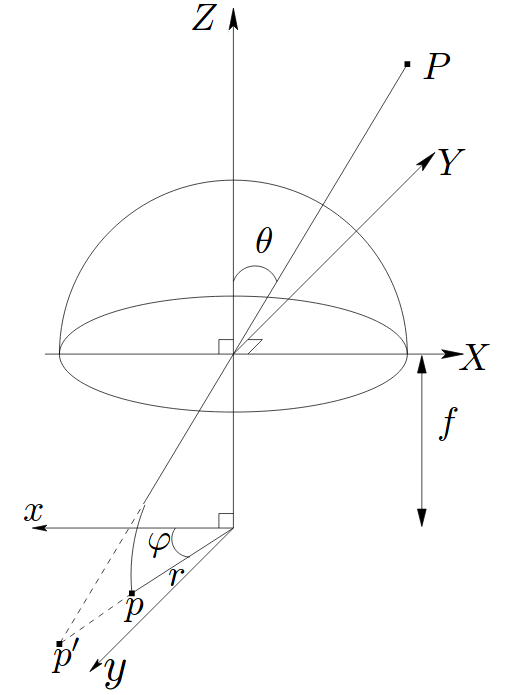
\includegraphics[width=0.5\textwidth]{figures/camera/generic_model.png}
    \label{fig:camera:generic}
\end{wrapfigure}

In this formulation, we can see that the difference between models is purely
the mapping from real-world angle to the camera principal vector. Also 
clearly evident is that the theoretical limit of the pinhole model lies at
$180\degree$ field of view, meaning $\pm90$ in any direction, which is when
$\tan$ diverges. On the other hand, stereographic projection can handle up to
$\pm180$ degrees in any direction before diverging.

\subsection{Tradeoffs}

 --------- Cut or trim down massively -----------

%Arguably, it is mostly human operators that care about the type of projection
%used in cameras. Computer vision algorithms can be developed that operate
%over each of the resulting types of distortions. 

Since I am to simulate localizing a vehicle's world position from the pixels
on the camera plane, and derive an associated localization error, I examine a bound
on localization accuracy in the form of ground area covered per pixel. That is,
in the worst case a vehicle will be contained within 1 pixel, so the ground
area covered by each pixel is an upper bound for localization error.

% TODO figure of different projections and areas covered, at straight down and 45 degrees
% TODO discuss these

The literature suggests that a good camera model should closely approximate
real cameras, and have useful mathematical properties~\cite{fleckperspective}.
Pinhole perspective projections preserve straight lines, but not circular
shapes as field of view widens. On the other hand, steregraphic models 
preserve circularity everywhere but not straight lines. The choice here
will depend on the type of algorithm selected.

\subsection{Conclusion}
 --------- Cut or trim down massively -----------

In order to be able to analyze the use of very wide fields of view, I 
implemented this unified model as a ray tracing module with a fixed
focal length of 0.1 meters, which according to~\cite{lumeneracamera}
is sometimes used in traffic cameras. Besides being able to select
the specific model to use, the resolution is allowed to vary,
as well as the horizontal and vertical maximum field of view.

However, while this section has presented alternative camera models, I will mostly
continue to use the pinhole model, unless the field of view is pushed beyond
90 degrees in either direction, in order to conform with the type of camera
most likely to be used in practice.

 
\section{Localization and Error}

As previously mentioned, the cameras deployed in the infrastructure will
send an estimated real world position to the vehicle as it travels through the 
camera's catchment area, reducing its positional uncertainty. This requires
deriving an accurate simulation how real-world cameras would perform this task.

\subsection{Approach}

In a real-world implementation of the proposed system, a camera would wirelessly
transmit estimated vehicle positions and associated uncertainty to vehicles in its field of view.

To enable position estimation, the camera needs to know its own world position and orientation, 
as well as the position and orientation of the ground plane. In in this work,
I assume the ground plane to be flat (a locally reasonable assumption, especially along roads), 
and equal to the $Z = 0$ plane. I report the position $(x,y)$ of the vehicle
as the estimated geometric center of the vehicle on the ground plane. 
Note that in practice, using the midpoint of the front or rear axle, rather than the center, 
may be a more consistent reference between vehicles.

Once the computer vision algorithm running on the camera estimates the center of the vehicle,
it must also be associated with an uncertainty. I simplify to a circular
error radius, $r$, which is transmitted as a $2\sigma^2I$ covariance 
with the state vector $(x,y)$. The error radius directly determines
the operational capability of the autonomous vehicles, thus must be
accurately represented.

There are three components that contribute to the error radius:
\begin{enumerate}
    \item Error in the camera's own location and orientation
    \item The algorithmic error in the estimation of the pixel that represents the estimated center of the vehicle
    \item The ground area covered by the pixel that represents the estimated center of the vehicle
\end{enumerate}
 
These will be analysed in turn. Note that I assume calibrated cameras without distortions, and no motion blur.

\subsection{Location and Orientation Error}

Of the three sources of error, this one is the most difficult to reason about. 
Many transport authorities have standard mounting specifications, including mount heights, for cameras~\cite{StreetscapeGuideance}.
However, none of these specify the tolerances in location and orientation, and we will have to make some educated guesses.

I assume that the position and orientation error is normally distributed, with
95\% of positions within 0.03 meters in any direction, 
and orientation within a 0.5 degree cone about the principal axis 95\% of the time.
In mathematical terms, this means $\Delta_{x}$, $\Delta_{y}$, and $\Delta_{z}$ 
are all sampled from $\mathcal{N}(0, (0.03/2)^2)$. The orientation error is given as
$\Delta_{orientation} \sim \mathcal{N}(0, (0.5/2)\degree2)$.
These tight bounds could be achieved using some sort of post-installation 
calibration procedure. 

%Orientation accuracy can be further improved by adding 
%an interial measurement unit to the camera, which on its own
%could provide better than $0.5\degree$ accuracy in the roll and raw directions according
%to~\cite{kok2017}.

To translate these values into an uncertainty on the ground plane, consider that
any horizontal camera movement ($\Delta_{x}$, $\Delta_{y}$) from its true position simply translates
the predicted vehicle location and therefore increases its error by the length of the translation.
I call this combined value $err_{xy}$ and at two standard deviations it is bounded above by
$\abs{err_{xy}} = 0.03$.

Vertical translation, $\Delta_z\sim \mathcal{N}(0, (0.03/2)^2)$
of the camera induces an error as $err_{z}(d, h) = \Delta_z \frac{d}{h}$ %, with variance $\sigma_{z}(d,h)^2 = (d/h)^2(0.03/2)^2$ 
where $d$ is the ground distance to the vehicle (on the XY plane), and $h$ is the true intended
height of the camera.

Thus, the total contribution from the camera's positional error to the error radius
will (95\% of the time) be bounded by $(err_{xy} + err_{z}(d, h))$, which evaluates to

\[ err_{xyz}(h, d) = 0.03 + \frac{0.03d}{h} \]

Similarly, it can be shown that using a conical error region about the desired principal axis
of magnitude $\Delta_{orientation} \sim \mathcal{N}(0,(0.5/2)\degree)$, 
for a camera at height $h$, and ground distance to the vehicle $d$, the
error induced in the estimation of the vehicle's center is 

\[ err_{orientation}(h, d) = h\tan(\tan^{-1}(d/h) + \Delta_{orientation}) - d \] %\frac{hd + h^2\Delta_{orientation}}{h - d\Delta_{orientation}} - d$.


***TODO graphic showing two types of orientation error to help reader visualize what is being calculated***


\subsection{Algorithmic Error}

The vehicle localization algorithm needs to scan the pixel plane for vehicles,
and return pixel representing the center of vehicles on the ground plane.
The center of the pixel projected onto the ground plane is taken as the vehicle center.

This process can be arbitrarily complex. I assume that at the time of deployment, 
computer vision algorithms are very good at this task, but may still
be wrong by several pixels. I analyze the effect of this inaccuracy
in the model validation Section~\ref{sec:camera:validation} and refer to the Euclidean distance
in the pixel plane from the true center pixel to the calculated one
as $\Delta_{alg} \sim \mathcal{N}(0, \eta_{alg}/2)$.

\subsection{Error from Camera Limitations}

Lastly, the error induced by the camera must be accounted for. Consider that 
in the limit, a vehicle is covered by exactly one pixel, meaning any estimate
of its position is at least as uncertain as the ground area 
covered by that pixel. On the other hand, if a vehicle
exactly fills the camera plane and the localization algorithm perfectly determines
the center of the vehicle in the pixel plane, the estimate still cannot
be better than the area covered by the single pixel.

I call the area covered by a pixel $p$, $A(p)$. $A(p)$ is also a function of the camera
position and orientation, and the camera parameters (field of view and resolution),
but these are omitted here as they are constant for any given camera.

Correspondingly, an approximate upper bound on the longest distance
within a pixel can be calculated as the diagonal of a square,
resulting in a ground distance of $err_{pixel}(p) = \sqrt{(2A(p))}$. 


\subsection{Complete Error Model}

I now combine the three sources of error to determine an approximate
error radius for the vehicle localization.

\[
    r(h,d,p) = err_{xyz}(h,d) + err_{orientation}(h,d) + \Delta_{alg}*err_{pixel}(p)
\]

For any individual camera, the $err_{xyz}$ and $err_{orientation}$ terms introduce
a directed bias for any point in the pixel plane, though over many installed cameras
these terms have a normal distribution. The $\Delta_{alg}$ is 
modeled as normal as well. To take advantage of this, I also multiply each with a tuning
parameter, related to their variances, which I use to trade off error bound size versus
error bound accuracy. The $err_{pixel}$ term is systematic i
and a complex function of camera parameters and estimated vehicle location, and
the only component with a non-zero mean over a large number of samples.

To validate $r$ in simulation, when a vehicle is visible to a camera,
I project the ground truth vehicle center to the (slightly-mispositioned) camera, which
automatically incorporates the positional and orientational errors.
The algorithmic error shifts the incident pixel a distance sampled according to the distribution 
of $\Delta_{alg}$, in a randomly sampled direction. 
Finally, the pixel error is computed from the area of the chosen pixel.

\section{Error Model Validation}
\label{sec:camera:validation}

In this section I evaluate the error radius function developed above. It is a good error model if,

\begin{enumerate}
    \item For a given estimated vehicle location, the true location should be within the predicted
          error radius most of the time. My formulation aims for 95\% accuracy.
    \item It is not over-conservative: the tighter the bound, the more useful the update is
          for vehicle navigation.
\end{enumerate}

I also examine how the different components that make up the error radius vary
as the pitch of the camera varies, followed by a brief look at the
effect of algorithmic inaccuracy. Experiments were performed
with the camera placed at a height of 6 meters above the ground, and a fixed
field of view of 60 degrees horizontally and vertically. Rotation about the Z axis
was ignored as it does not affect results.

\subsection{Quality of $r$ as an Error Bound}

For this and the following subsection I assume a perfect algorithm,
setting $\Delta_{alg}$ to 1.

\begin{table}[htb]
    \centering
    \caption[$r$ as an ErrorBound]{Success Rate of $r$ as an Error Bound}
    \label{tab:camera:bound accuracy}
    \begin{tabular}{@{}ccc@{}}
        \toprule
        Total Samples & \# Within Error Bound & \% Within Error Bound \\ \midrule
        125000        & 123865                     & 99.092               
    \end{tabular}
\end{table}

Table~\ref{tab:camera:bound accuracy} shows that more than 99\% of 125000 sampled camera positions
and vehicle positions, the distance from the predicted vehicle position to 
its actual position is within is within the calculated error radius. This
is actually better than intended, since the construction was for 95\% accuracy.

It is easy to achieve an error bound that is always valid: simply set it very high.
Figure \ref{fig:camera:diff bound error} shows two important characteristics. Firstly, the difference between
the predicted error radius and the actual error distance is small, meaning
it is not an excessively high bound. Secondly, when the bound is \textit{incorrect} (very small region less than zero in blue)
the true error only slightly exceeds the error bound.

\begin{figure}[htb]
    \begin{center}
        %% Creator: Matplotlib, PGF backend
%%
%% To include the figure in your LaTeX document, write
%%   \input{<filename>.pgf}
%%
%% Make sure the required packages are loaded in your preamble
%%   \usepackage{pgf}
%%
%% Figures using additional raster images can only be included by \input if
%% they are in the same directory as the main LaTeX file. For loading figures
%% from other directories you can use the `import` package
%%   \usepackage{import}
%% and then include the figures with
%%   \import{<path to file>}{<filename>.pgf}
%%
%% Matplotlib used the following preamble
%%   \usepackage{fontspec}
%%
\begingroup%
\makeatletter%
\begin{pgfpicture}%
\pgfpathrectangle{\pgfpointorigin}{\pgfqpoint{5.900000in}{2.900000in}}%
\pgfusepath{use as bounding box, clip}%
\begin{pgfscope}%
\pgfsetbuttcap%
\pgfsetmiterjoin%
\definecolor{currentfill}{rgb}{1.000000,1.000000,1.000000}%
\pgfsetfillcolor{currentfill}%
\pgfsetlinewidth{0.000000pt}%
\definecolor{currentstroke}{rgb}{1.000000,1.000000,1.000000}%
\pgfsetstrokecolor{currentstroke}%
\pgfsetdash{}{0pt}%
\pgfpathmoveto{\pgfqpoint{0.000000in}{-0.000000in}}%
\pgfpathlineto{\pgfqpoint{5.900000in}{-0.000000in}}%
\pgfpathlineto{\pgfqpoint{5.900000in}{2.900000in}}%
\pgfpathlineto{\pgfqpoint{0.000000in}{2.900000in}}%
\pgfpathclose%
\pgfusepath{fill}%
\end{pgfscope}%
\begin{pgfscope}%
\pgfsetbuttcap%
\pgfsetmiterjoin%
\definecolor{currentfill}{rgb}{1.000000,1.000000,1.000000}%
\pgfsetfillcolor{currentfill}%
\pgfsetlinewidth{0.000000pt}%
\definecolor{currentstroke}{rgb}{0.000000,0.000000,0.000000}%
\pgfsetstrokecolor{currentstroke}%
\pgfsetstrokeopacity{0.000000}%
\pgfsetdash{}{0pt}%
\pgfpathmoveto{\pgfqpoint{0.748001in}{0.542944in}}%
\pgfpathlineto{\pgfqpoint{5.711265in}{0.542944in}}%
\pgfpathlineto{\pgfqpoint{5.711265in}{2.765000in}}%
\pgfpathlineto{\pgfqpoint{0.748001in}{2.765000in}}%
\pgfpathclose%
\pgfusepath{fill}%
\end{pgfscope}%
\begin{pgfscope}%
\pgfpathrectangle{\pgfqpoint{0.748001in}{0.542944in}}{\pgfqpoint{4.963264in}{2.222056in}} %
\pgfusepath{clip}%
\pgfsetrectcap%
\pgfsetroundjoin%
\pgfsetlinewidth{0.803000pt}%
\definecolor{currentstroke}{rgb}{0.900000,0.900000,0.900000}%
\pgfsetstrokecolor{currentstroke}%
\pgfsetdash{}{0pt}%
\pgfpathmoveto{\pgfqpoint{0.748001in}{0.542944in}}%
\pgfpathlineto{\pgfqpoint{0.748001in}{2.765000in}}%
\pgfusepath{stroke}%
\end{pgfscope}%
\begin{pgfscope}%
\pgfsetbuttcap%
\pgfsetroundjoin%
\definecolor{currentfill}{rgb}{0.333333,0.333333,0.333333}%
\pgfsetfillcolor{currentfill}%
\pgfsetlinewidth{0.803000pt}%
\definecolor{currentstroke}{rgb}{0.333333,0.333333,0.333333}%
\pgfsetstrokecolor{currentstroke}%
\pgfsetdash{}{0pt}%
\pgfsys@defobject{currentmarker}{\pgfqpoint{0.000000in}{-0.048611in}}{\pgfqpoint{0.000000in}{0.000000in}}{%
\pgfpathmoveto{\pgfqpoint{0.000000in}{0.000000in}}%
\pgfpathlineto{\pgfqpoint{0.000000in}{-0.048611in}}%
\pgfusepath{stroke,fill}%
}%
\begin{pgfscope}%
\pgfsys@transformshift{0.748001in}{0.542944in}%
\pgfsys@useobject{currentmarker}{}%
\end{pgfscope}%
\end{pgfscope}%
\begin{pgfscope}%
\definecolor{textcolor}{rgb}{0.333333,0.333333,0.333333}%
\pgfsetstrokecolor{textcolor}%
\pgfsetfillcolor{textcolor}%
\pgftext[x=0.748001in,y=0.445722in,,top]{\color{textcolor}\rmfamily\fontsize{10.000000}{12.000000}\selectfont \(\displaystyle -0.4\)}%
\end{pgfscope}%
\begin{pgfscope}%
\pgfpathrectangle{\pgfqpoint{0.748001in}{0.542944in}}{\pgfqpoint{4.963264in}{2.222056in}} %
\pgfusepath{clip}%
\pgfsetrectcap%
\pgfsetroundjoin%
\pgfsetlinewidth{0.803000pt}%
\definecolor{currentstroke}{rgb}{0.900000,0.900000,0.900000}%
\pgfsetstrokecolor{currentstroke}%
\pgfsetdash{}{0pt}%
\pgfpathmoveto{\pgfqpoint{1.457039in}{0.542944in}}%
\pgfpathlineto{\pgfqpoint{1.457039in}{2.765000in}}%
\pgfusepath{stroke}%
\end{pgfscope}%
\begin{pgfscope}%
\pgfsetbuttcap%
\pgfsetroundjoin%
\definecolor{currentfill}{rgb}{0.333333,0.333333,0.333333}%
\pgfsetfillcolor{currentfill}%
\pgfsetlinewidth{0.803000pt}%
\definecolor{currentstroke}{rgb}{0.333333,0.333333,0.333333}%
\pgfsetstrokecolor{currentstroke}%
\pgfsetdash{}{0pt}%
\pgfsys@defobject{currentmarker}{\pgfqpoint{0.000000in}{-0.048611in}}{\pgfqpoint{0.000000in}{0.000000in}}{%
\pgfpathmoveto{\pgfqpoint{0.000000in}{0.000000in}}%
\pgfpathlineto{\pgfqpoint{0.000000in}{-0.048611in}}%
\pgfusepath{stroke,fill}%
}%
\begin{pgfscope}%
\pgfsys@transformshift{1.457039in}{0.542944in}%
\pgfsys@useobject{currentmarker}{}%
\end{pgfscope}%
\end{pgfscope}%
\begin{pgfscope}%
\definecolor{textcolor}{rgb}{0.333333,0.333333,0.333333}%
\pgfsetstrokecolor{textcolor}%
\pgfsetfillcolor{textcolor}%
\pgftext[x=1.457039in,y=0.445722in,,top]{\color{textcolor}\rmfamily\fontsize{10.000000}{12.000000}\selectfont \(\displaystyle -0.2\)}%
\end{pgfscope}%
\begin{pgfscope}%
\pgfpathrectangle{\pgfqpoint{0.748001in}{0.542944in}}{\pgfqpoint{4.963264in}{2.222056in}} %
\pgfusepath{clip}%
\pgfsetrectcap%
\pgfsetroundjoin%
\pgfsetlinewidth{0.803000pt}%
\definecolor{currentstroke}{rgb}{0.900000,0.900000,0.900000}%
\pgfsetstrokecolor{currentstroke}%
\pgfsetdash{}{0pt}%
\pgfpathmoveto{\pgfqpoint{2.166076in}{0.542944in}}%
\pgfpathlineto{\pgfqpoint{2.166076in}{2.765000in}}%
\pgfusepath{stroke}%
\end{pgfscope}%
\begin{pgfscope}%
\pgfsetbuttcap%
\pgfsetroundjoin%
\definecolor{currentfill}{rgb}{0.333333,0.333333,0.333333}%
\pgfsetfillcolor{currentfill}%
\pgfsetlinewidth{0.803000pt}%
\definecolor{currentstroke}{rgb}{0.333333,0.333333,0.333333}%
\pgfsetstrokecolor{currentstroke}%
\pgfsetdash{}{0pt}%
\pgfsys@defobject{currentmarker}{\pgfqpoint{0.000000in}{-0.048611in}}{\pgfqpoint{0.000000in}{0.000000in}}{%
\pgfpathmoveto{\pgfqpoint{0.000000in}{0.000000in}}%
\pgfpathlineto{\pgfqpoint{0.000000in}{-0.048611in}}%
\pgfusepath{stroke,fill}%
}%
\begin{pgfscope}%
\pgfsys@transformshift{2.166076in}{0.542944in}%
\pgfsys@useobject{currentmarker}{}%
\end{pgfscope}%
\end{pgfscope}%
\begin{pgfscope}%
\definecolor{textcolor}{rgb}{0.333333,0.333333,0.333333}%
\pgfsetstrokecolor{textcolor}%
\pgfsetfillcolor{textcolor}%
\pgftext[x=2.166076in,y=0.445722in,,top]{\color{textcolor}\rmfamily\fontsize{10.000000}{12.000000}\selectfont \(\displaystyle 0.0\)}%
\end{pgfscope}%
\begin{pgfscope}%
\pgfpathrectangle{\pgfqpoint{0.748001in}{0.542944in}}{\pgfqpoint{4.963264in}{2.222056in}} %
\pgfusepath{clip}%
\pgfsetrectcap%
\pgfsetroundjoin%
\pgfsetlinewidth{0.803000pt}%
\definecolor{currentstroke}{rgb}{0.900000,0.900000,0.900000}%
\pgfsetstrokecolor{currentstroke}%
\pgfsetdash{}{0pt}%
\pgfpathmoveto{\pgfqpoint{2.875114in}{0.542944in}}%
\pgfpathlineto{\pgfqpoint{2.875114in}{2.765000in}}%
\pgfusepath{stroke}%
\end{pgfscope}%
\begin{pgfscope}%
\pgfsetbuttcap%
\pgfsetroundjoin%
\definecolor{currentfill}{rgb}{0.333333,0.333333,0.333333}%
\pgfsetfillcolor{currentfill}%
\pgfsetlinewidth{0.803000pt}%
\definecolor{currentstroke}{rgb}{0.333333,0.333333,0.333333}%
\pgfsetstrokecolor{currentstroke}%
\pgfsetdash{}{0pt}%
\pgfsys@defobject{currentmarker}{\pgfqpoint{0.000000in}{-0.048611in}}{\pgfqpoint{0.000000in}{0.000000in}}{%
\pgfpathmoveto{\pgfqpoint{0.000000in}{0.000000in}}%
\pgfpathlineto{\pgfqpoint{0.000000in}{-0.048611in}}%
\pgfusepath{stroke,fill}%
}%
\begin{pgfscope}%
\pgfsys@transformshift{2.875114in}{0.542944in}%
\pgfsys@useobject{currentmarker}{}%
\end{pgfscope}%
\end{pgfscope}%
\begin{pgfscope}%
\definecolor{textcolor}{rgb}{0.333333,0.333333,0.333333}%
\pgfsetstrokecolor{textcolor}%
\pgfsetfillcolor{textcolor}%
\pgftext[x=2.875114in,y=0.445722in,,top]{\color{textcolor}\rmfamily\fontsize{10.000000}{12.000000}\selectfont \(\displaystyle 0.2\)}%
\end{pgfscope}%
\begin{pgfscope}%
\pgfpathrectangle{\pgfqpoint{0.748001in}{0.542944in}}{\pgfqpoint{4.963264in}{2.222056in}} %
\pgfusepath{clip}%
\pgfsetrectcap%
\pgfsetroundjoin%
\pgfsetlinewidth{0.803000pt}%
\definecolor{currentstroke}{rgb}{0.900000,0.900000,0.900000}%
\pgfsetstrokecolor{currentstroke}%
\pgfsetdash{}{0pt}%
\pgfpathmoveto{\pgfqpoint{3.584152in}{0.542944in}}%
\pgfpathlineto{\pgfqpoint{3.584152in}{2.765000in}}%
\pgfusepath{stroke}%
\end{pgfscope}%
\begin{pgfscope}%
\pgfsetbuttcap%
\pgfsetroundjoin%
\definecolor{currentfill}{rgb}{0.333333,0.333333,0.333333}%
\pgfsetfillcolor{currentfill}%
\pgfsetlinewidth{0.803000pt}%
\definecolor{currentstroke}{rgb}{0.333333,0.333333,0.333333}%
\pgfsetstrokecolor{currentstroke}%
\pgfsetdash{}{0pt}%
\pgfsys@defobject{currentmarker}{\pgfqpoint{0.000000in}{-0.048611in}}{\pgfqpoint{0.000000in}{0.000000in}}{%
\pgfpathmoveto{\pgfqpoint{0.000000in}{0.000000in}}%
\pgfpathlineto{\pgfqpoint{0.000000in}{-0.048611in}}%
\pgfusepath{stroke,fill}%
}%
\begin{pgfscope}%
\pgfsys@transformshift{3.584152in}{0.542944in}%
\pgfsys@useobject{currentmarker}{}%
\end{pgfscope}%
\end{pgfscope}%
\begin{pgfscope}%
\definecolor{textcolor}{rgb}{0.333333,0.333333,0.333333}%
\pgfsetstrokecolor{textcolor}%
\pgfsetfillcolor{textcolor}%
\pgftext[x=3.584152in,y=0.445722in,,top]{\color{textcolor}\rmfamily\fontsize{10.000000}{12.000000}\selectfont \(\displaystyle 0.4\)}%
\end{pgfscope}%
\begin{pgfscope}%
\pgfpathrectangle{\pgfqpoint{0.748001in}{0.542944in}}{\pgfqpoint{4.963264in}{2.222056in}} %
\pgfusepath{clip}%
\pgfsetrectcap%
\pgfsetroundjoin%
\pgfsetlinewidth{0.803000pt}%
\definecolor{currentstroke}{rgb}{0.900000,0.900000,0.900000}%
\pgfsetstrokecolor{currentstroke}%
\pgfsetdash{}{0pt}%
\pgfpathmoveto{\pgfqpoint{4.293190in}{0.542944in}}%
\pgfpathlineto{\pgfqpoint{4.293190in}{2.765000in}}%
\pgfusepath{stroke}%
\end{pgfscope}%
\begin{pgfscope}%
\pgfsetbuttcap%
\pgfsetroundjoin%
\definecolor{currentfill}{rgb}{0.333333,0.333333,0.333333}%
\pgfsetfillcolor{currentfill}%
\pgfsetlinewidth{0.803000pt}%
\definecolor{currentstroke}{rgb}{0.333333,0.333333,0.333333}%
\pgfsetstrokecolor{currentstroke}%
\pgfsetdash{}{0pt}%
\pgfsys@defobject{currentmarker}{\pgfqpoint{0.000000in}{-0.048611in}}{\pgfqpoint{0.000000in}{0.000000in}}{%
\pgfpathmoveto{\pgfqpoint{0.000000in}{0.000000in}}%
\pgfpathlineto{\pgfqpoint{0.000000in}{-0.048611in}}%
\pgfusepath{stroke,fill}%
}%
\begin{pgfscope}%
\pgfsys@transformshift{4.293190in}{0.542944in}%
\pgfsys@useobject{currentmarker}{}%
\end{pgfscope}%
\end{pgfscope}%
\begin{pgfscope}%
\definecolor{textcolor}{rgb}{0.333333,0.333333,0.333333}%
\pgfsetstrokecolor{textcolor}%
\pgfsetfillcolor{textcolor}%
\pgftext[x=4.293190in,y=0.445722in,,top]{\color{textcolor}\rmfamily\fontsize{10.000000}{12.000000}\selectfont \(\displaystyle 0.6\)}%
\end{pgfscope}%
\begin{pgfscope}%
\pgfpathrectangle{\pgfqpoint{0.748001in}{0.542944in}}{\pgfqpoint{4.963264in}{2.222056in}} %
\pgfusepath{clip}%
\pgfsetrectcap%
\pgfsetroundjoin%
\pgfsetlinewidth{0.803000pt}%
\definecolor{currentstroke}{rgb}{0.900000,0.900000,0.900000}%
\pgfsetstrokecolor{currentstroke}%
\pgfsetdash{}{0pt}%
\pgfpathmoveto{\pgfqpoint{5.002227in}{0.542944in}}%
\pgfpathlineto{\pgfqpoint{5.002227in}{2.765000in}}%
\pgfusepath{stroke}%
\end{pgfscope}%
\begin{pgfscope}%
\pgfsetbuttcap%
\pgfsetroundjoin%
\definecolor{currentfill}{rgb}{0.333333,0.333333,0.333333}%
\pgfsetfillcolor{currentfill}%
\pgfsetlinewidth{0.803000pt}%
\definecolor{currentstroke}{rgb}{0.333333,0.333333,0.333333}%
\pgfsetstrokecolor{currentstroke}%
\pgfsetdash{}{0pt}%
\pgfsys@defobject{currentmarker}{\pgfqpoint{0.000000in}{-0.048611in}}{\pgfqpoint{0.000000in}{0.000000in}}{%
\pgfpathmoveto{\pgfqpoint{0.000000in}{0.000000in}}%
\pgfpathlineto{\pgfqpoint{0.000000in}{-0.048611in}}%
\pgfusepath{stroke,fill}%
}%
\begin{pgfscope}%
\pgfsys@transformshift{5.002227in}{0.542944in}%
\pgfsys@useobject{currentmarker}{}%
\end{pgfscope}%
\end{pgfscope}%
\begin{pgfscope}%
\definecolor{textcolor}{rgb}{0.333333,0.333333,0.333333}%
\pgfsetstrokecolor{textcolor}%
\pgfsetfillcolor{textcolor}%
\pgftext[x=5.002227in,y=0.445722in,,top]{\color{textcolor}\rmfamily\fontsize{10.000000}{12.000000}\selectfont \(\displaystyle 0.8\)}%
\end{pgfscope}%
\begin{pgfscope}%
\pgfpathrectangle{\pgfqpoint{0.748001in}{0.542944in}}{\pgfqpoint{4.963264in}{2.222056in}} %
\pgfusepath{clip}%
\pgfsetrectcap%
\pgfsetroundjoin%
\pgfsetlinewidth{0.803000pt}%
\definecolor{currentstroke}{rgb}{0.900000,0.900000,0.900000}%
\pgfsetstrokecolor{currentstroke}%
\pgfsetdash{}{0pt}%
\pgfpathmoveto{\pgfqpoint{5.711265in}{0.542944in}}%
\pgfpathlineto{\pgfqpoint{5.711265in}{2.765000in}}%
\pgfusepath{stroke}%
\end{pgfscope}%
\begin{pgfscope}%
\pgfsetbuttcap%
\pgfsetroundjoin%
\definecolor{currentfill}{rgb}{0.333333,0.333333,0.333333}%
\pgfsetfillcolor{currentfill}%
\pgfsetlinewidth{0.803000pt}%
\definecolor{currentstroke}{rgb}{0.333333,0.333333,0.333333}%
\pgfsetstrokecolor{currentstroke}%
\pgfsetdash{}{0pt}%
\pgfsys@defobject{currentmarker}{\pgfqpoint{0.000000in}{-0.048611in}}{\pgfqpoint{0.000000in}{0.000000in}}{%
\pgfpathmoveto{\pgfqpoint{0.000000in}{0.000000in}}%
\pgfpathlineto{\pgfqpoint{0.000000in}{-0.048611in}}%
\pgfusepath{stroke,fill}%
}%
\begin{pgfscope}%
\pgfsys@transformshift{5.711265in}{0.542944in}%
\pgfsys@useobject{currentmarker}{}%
\end{pgfscope}%
\end{pgfscope}%
\begin{pgfscope}%
\definecolor{textcolor}{rgb}{0.333333,0.333333,0.333333}%
\pgfsetstrokecolor{textcolor}%
\pgfsetfillcolor{textcolor}%
\pgftext[x=5.711265in,y=0.445722in,,top]{\color{textcolor}\rmfamily\fontsize{10.000000}{12.000000}\selectfont \(\displaystyle 1.0\)}%
\end{pgfscope}%
\begin{pgfscope}%
\definecolor{textcolor}{rgb}{0.333333,0.333333,0.333333}%
\pgfsetstrokecolor{textcolor}%
\pgfsetfillcolor{textcolor}%
\pgftext[x=3.229633in,y=0.266833in,,top]{\color{textcolor}\rmfamily\fontsize{12.000000}{14.400000}\selectfont Difference (Error Radius - True Error)}%
\end{pgfscope}%
\begin{pgfscope}%
\pgfpathrectangle{\pgfqpoint{0.748001in}{0.542944in}}{\pgfqpoint{4.963264in}{2.222056in}} %
\pgfusepath{clip}%
\pgfsetrectcap%
\pgfsetroundjoin%
\pgfsetlinewidth{0.803000pt}%
\definecolor{currentstroke}{rgb}{0.900000,0.900000,0.900000}%
\pgfsetstrokecolor{currentstroke}%
\pgfsetdash{}{0pt}%
\pgfpathmoveto{\pgfqpoint{0.748001in}{0.542944in}}%
\pgfpathlineto{\pgfqpoint{5.711265in}{0.542944in}}%
\pgfusepath{stroke}%
\end{pgfscope}%
\begin{pgfscope}%
\pgfsetbuttcap%
\pgfsetroundjoin%
\definecolor{currentfill}{rgb}{0.333333,0.333333,0.333333}%
\pgfsetfillcolor{currentfill}%
\pgfsetlinewidth{0.803000pt}%
\definecolor{currentstroke}{rgb}{0.333333,0.333333,0.333333}%
\pgfsetstrokecolor{currentstroke}%
\pgfsetdash{}{0pt}%
\pgfsys@defobject{currentmarker}{\pgfqpoint{-0.048611in}{0.000000in}}{\pgfqpoint{0.000000in}{0.000000in}}{%
\pgfpathmoveto{\pgfqpoint{0.000000in}{0.000000in}}%
\pgfpathlineto{\pgfqpoint{-0.048611in}{0.000000in}}%
\pgfusepath{stroke,fill}%
}%
\begin{pgfscope}%
\pgfsys@transformshift{0.748001in}{0.542944in}%
\pgfsys@useobject{currentmarker}{}%
\end{pgfscope}%
\end{pgfscope}%
\begin{pgfscope}%
\definecolor{textcolor}{rgb}{0.333333,0.333333,0.333333}%
\pgfsetstrokecolor{textcolor}%
\pgfsetfillcolor{textcolor}%
\pgftext[x=0.581334in,y=0.494750in,left,base]{\color{textcolor}\rmfamily\fontsize{10.000000}{12.000000}\selectfont \(\displaystyle 0\)}%
\end{pgfscope}%
\begin{pgfscope}%
\pgfpathrectangle{\pgfqpoint{0.748001in}{0.542944in}}{\pgfqpoint{4.963264in}{2.222056in}} %
\pgfusepath{clip}%
\pgfsetrectcap%
\pgfsetroundjoin%
\pgfsetlinewidth{0.803000pt}%
\definecolor{currentstroke}{rgb}{0.900000,0.900000,0.900000}%
\pgfsetstrokecolor{currentstroke}%
\pgfsetdash{}{0pt}%
\pgfpathmoveto{\pgfqpoint{0.748001in}{0.881527in}}%
\pgfpathlineto{\pgfqpoint{5.711265in}{0.881527in}}%
\pgfusepath{stroke}%
\end{pgfscope}%
\begin{pgfscope}%
\pgfsetbuttcap%
\pgfsetroundjoin%
\definecolor{currentfill}{rgb}{0.333333,0.333333,0.333333}%
\pgfsetfillcolor{currentfill}%
\pgfsetlinewidth{0.803000pt}%
\definecolor{currentstroke}{rgb}{0.333333,0.333333,0.333333}%
\pgfsetstrokecolor{currentstroke}%
\pgfsetdash{}{0pt}%
\pgfsys@defobject{currentmarker}{\pgfqpoint{-0.048611in}{0.000000in}}{\pgfqpoint{0.000000in}{0.000000in}}{%
\pgfpathmoveto{\pgfqpoint{0.000000in}{0.000000in}}%
\pgfpathlineto{\pgfqpoint{-0.048611in}{0.000000in}}%
\pgfusepath{stroke,fill}%
}%
\begin{pgfscope}%
\pgfsys@transformshift{0.748001in}{0.881527in}%
\pgfsys@useobject{currentmarker}{}%
\end{pgfscope}%
\end{pgfscope}%
\begin{pgfscope}%
\definecolor{textcolor}{rgb}{0.333333,0.333333,0.333333}%
\pgfsetstrokecolor{textcolor}%
\pgfsetfillcolor{textcolor}%
\pgftext[x=0.303555in,y=0.833332in,left,base]{\color{textcolor}\rmfamily\fontsize{10.000000}{12.000000}\selectfont \(\displaystyle 10000\)}%
\end{pgfscope}%
\begin{pgfscope}%
\pgfpathrectangle{\pgfqpoint{0.748001in}{0.542944in}}{\pgfqpoint{4.963264in}{2.222056in}} %
\pgfusepath{clip}%
\pgfsetrectcap%
\pgfsetroundjoin%
\pgfsetlinewidth{0.803000pt}%
\definecolor{currentstroke}{rgb}{0.900000,0.900000,0.900000}%
\pgfsetstrokecolor{currentstroke}%
\pgfsetdash{}{0pt}%
\pgfpathmoveto{\pgfqpoint{0.748001in}{1.220110in}}%
\pgfpathlineto{\pgfqpoint{5.711265in}{1.220110in}}%
\pgfusepath{stroke}%
\end{pgfscope}%
\begin{pgfscope}%
\pgfsetbuttcap%
\pgfsetroundjoin%
\definecolor{currentfill}{rgb}{0.333333,0.333333,0.333333}%
\pgfsetfillcolor{currentfill}%
\pgfsetlinewidth{0.803000pt}%
\definecolor{currentstroke}{rgb}{0.333333,0.333333,0.333333}%
\pgfsetstrokecolor{currentstroke}%
\pgfsetdash{}{0pt}%
\pgfsys@defobject{currentmarker}{\pgfqpoint{-0.048611in}{0.000000in}}{\pgfqpoint{0.000000in}{0.000000in}}{%
\pgfpathmoveto{\pgfqpoint{0.000000in}{0.000000in}}%
\pgfpathlineto{\pgfqpoint{-0.048611in}{0.000000in}}%
\pgfusepath{stroke,fill}%
}%
\begin{pgfscope}%
\pgfsys@transformshift{0.748001in}{1.220110in}%
\pgfsys@useobject{currentmarker}{}%
\end{pgfscope}%
\end{pgfscope}%
\begin{pgfscope}%
\definecolor{textcolor}{rgb}{0.333333,0.333333,0.333333}%
\pgfsetstrokecolor{textcolor}%
\pgfsetfillcolor{textcolor}%
\pgftext[x=0.303555in,y=1.171915in,left,base]{\color{textcolor}\rmfamily\fontsize{10.000000}{12.000000}\selectfont \(\displaystyle 20000\)}%
\end{pgfscope}%
\begin{pgfscope}%
\pgfpathrectangle{\pgfqpoint{0.748001in}{0.542944in}}{\pgfqpoint{4.963264in}{2.222056in}} %
\pgfusepath{clip}%
\pgfsetrectcap%
\pgfsetroundjoin%
\pgfsetlinewidth{0.803000pt}%
\definecolor{currentstroke}{rgb}{0.900000,0.900000,0.900000}%
\pgfsetstrokecolor{currentstroke}%
\pgfsetdash{}{0pt}%
\pgfpathmoveto{\pgfqpoint{0.748001in}{1.558692in}}%
\pgfpathlineto{\pgfqpoint{5.711265in}{1.558692in}}%
\pgfusepath{stroke}%
\end{pgfscope}%
\begin{pgfscope}%
\pgfsetbuttcap%
\pgfsetroundjoin%
\definecolor{currentfill}{rgb}{0.333333,0.333333,0.333333}%
\pgfsetfillcolor{currentfill}%
\pgfsetlinewidth{0.803000pt}%
\definecolor{currentstroke}{rgb}{0.333333,0.333333,0.333333}%
\pgfsetstrokecolor{currentstroke}%
\pgfsetdash{}{0pt}%
\pgfsys@defobject{currentmarker}{\pgfqpoint{-0.048611in}{0.000000in}}{\pgfqpoint{0.000000in}{0.000000in}}{%
\pgfpathmoveto{\pgfqpoint{0.000000in}{0.000000in}}%
\pgfpathlineto{\pgfqpoint{-0.048611in}{0.000000in}}%
\pgfusepath{stroke,fill}%
}%
\begin{pgfscope}%
\pgfsys@transformshift{0.748001in}{1.558692in}%
\pgfsys@useobject{currentmarker}{}%
\end{pgfscope}%
\end{pgfscope}%
\begin{pgfscope}%
\definecolor{textcolor}{rgb}{0.333333,0.333333,0.333333}%
\pgfsetstrokecolor{textcolor}%
\pgfsetfillcolor{textcolor}%
\pgftext[x=0.303555in,y=1.510498in,left,base]{\color{textcolor}\rmfamily\fontsize{10.000000}{12.000000}\selectfont \(\displaystyle 30000\)}%
\end{pgfscope}%
\begin{pgfscope}%
\pgfpathrectangle{\pgfqpoint{0.748001in}{0.542944in}}{\pgfqpoint{4.963264in}{2.222056in}} %
\pgfusepath{clip}%
\pgfsetrectcap%
\pgfsetroundjoin%
\pgfsetlinewidth{0.803000pt}%
\definecolor{currentstroke}{rgb}{0.900000,0.900000,0.900000}%
\pgfsetstrokecolor{currentstroke}%
\pgfsetdash{}{0pt}%
\pgfpathmoveto{\pgfqpoint{0.748001in}{1.897275in}}%
\pgfpathlineto{\pgfqpoint{5.711265in}{1.897275in}}%
\pgfusepath{stroke}%
\end{pgfscope}%
\begin{pgfscope}%
\pgfsetbuttcap%
\pgfsetroundjoin%
\definecolor{currentfill}{rgb}{0.333333,0.333333,0.333333}%
\pgfsetfillcolor{currentfill}%
\pgfsetlinewidth{0.803000pt}%
\definecolor{currentstroke}{rgb}{0.333333,0.333333,0.333333}%
\pgfsetstrokecolor{currentstroke}%
\pgfsetdash{}{0pt}%
\pgfsys@defobject{currentmarker}{\pgfqpoint{-0.048611in}{0.000000in}}{\pgfqpoint{0.000000in}{0.000000in}}{%
\pgfpathmoveto{\pgfqpoint{0.000000in}{0.000000in}}%
\pgfpathlineto{\pgfqpoint{-0.048611in}{0.000000in}}%
\pgfusepath{stroke,fill}%
}%
\begin{pgfscope}%
\pgfsys@transformshift{0.748001in}{1.897275in}%
\pgfsys@useobject{currentmarker}{}%
\end{pgfscope}%
\end{pgfscope}%
\begin{pgfscope}%
\definecolor{textcolor}{rgb}{0.333333,0.333333,0.333333}%
\pgfsetstrokecolor{textcolor}%
\pgfsetfillcolor{textcolor}%
\pgftext[x=0.303555in,y=1.849081in,left,base]{\color{textcolor}\rmfamily\fontsize{10.000000}{12.000000}\selectfont \(\displaystyle 40000\)}%
\end{pgfscope}%
\begin{pgfscope}%
\pgfpathrectangle{\pgfqpoint{0.748001in}{0.542944in}}{\pgfqpoint{4.963264in}{2.222056in}} %
\pgfusepath{clip}%
\pgfsetrectcap%
\pgfsetroundjoin%
\pgfsetlinewidth{0.803000pt}%
\definecolor{currentstroke}{rgb}{0.900000,0.900000,0.900000}%
\pgfsetstrokecolor{currentstroke}%
\pgfsetdash{}{0pt}%
\pgfpathmoveto{\pgfqpoint{0.748001in}{2.235858in}}%
\pgfpathlineto{\pgfqpoint{5.711265in}{2.235858in}}%
\pgfusepath{stroke}%
\end{pgfscope}%
\begin{pgfscope}%
\pgfsetbuttcap%
\pgfsetroundjoin%
\definecolor{currentfill}{rgb}{0.333333,0.333333,0.333333}%
\pgfsetfillcolor{currentfill}%
\pgfsetlinewidth{0.803000pt}%
\definecolor{currentstroke}{rgb}{0.333333,0.333333,0.333333}%
\pgfsetstrokecolor{currentstroke}%
\pgfsetdash{}{0pt}%
\pgfsys@defobject{currentmarker}{\pgfqpoint{-0.048611in}{0.000000in}}{\pgfqpoint{0.000000in}{0.000000in}}{%
\pgfpathmoveto{\pgfqpoint{0.000000in}{0.000000in}}%
\pgfpathlineto{\pgfqpoint{-0.048611in}{0.000000in}}%
\pgfusepath{stroke,fill}%
}%
\begin{pgfscope}%
\pgfsys@transformshift{0.748001in}{2.235858in}%
\pgfsys@useobject{currentmarker}{}%
\end{pgfscope}%
\end{pgfscope}%
\begin{pgfscope}%
\definecolor{textcolor}{rgb}{0.333333,0.333333,0.333333}%
\pgfsetstrokecolor{textcolor}%
\pgfsetfillcolor{textcolor}%
\pgftext[x=0.303555in,y=2.187663in,left,base]{\color{textcolor}\rmfamily\fontsize{10.000000}{12.000000}\selectfont \(\displaystyle 50000\)}%
\end{pgfscope}%
\begin{pgfscope}%
\pgfpathrectangle{\pgfqpoint{0.748001in}{0.542944in}}{\pgfqpoint{4.963264in}{2.222056in}} %
\pgfusepath{clip}%
\pgfsetrectcap%
\pgfsetroundjoin%
\pgfsetlinewidth{0.803000pt}%
\definecolor{currentstroke}{rgb}{0.900000,0.900000,0.900000}%
\pgfsetstrokecolor{currentstroke}%
\pgfsetdash{}{0pt}%
\pgfpathmoveto{\pgfqpoint{0.748001in}{2.574441in}}%
\pgfpathlineto{\pgfqpoint{5.711265in}{2.574441in}}%
\pgfusepath{stroke}%
\end{pgfscope}%
\begin{pgfscope}%
\pgfsetbuttcap%
\pgfsetroundjoin%
\definecolor{currentfill}{rgb}{0.333333,0.333333,0.333333}%
\pgfsetfillcolor{currentfill}%
\pgfsetlinewidth{0.803000pt}%
\definecolor{currentstroke}{rgb}{0.333333,0.333333,0.333333}%
\pgfsetstrokecolor{currentstroke}%
\pgfsetdash{}{0pt}%
\pgfsys@defobject{currentmarker}{\pgfqpoint{-0.048611in}{0.000000in}}{\pgfqpoint{0.000000in}{0.000000in}}{%
\pgfpathmoveto{\pgfqpoint{0.000000in}{0.000000in}}%
\pgfpathlineto{\pgfqpoint{-0.048611in}{0.000000in}}%
\pgfusepath{stroke,fill}%
}%
\begin{pgfscope}%
\pgfsys@transformshift{0.748001in}{2.574441in}%
\pgfsys@useobject{currentmarker}{}%
\end{pgfscope}%
\end{pgfscope}%
\begin{pgfscope}%
\definecolor{textcolor}{rgb}{0.333333,0.333333,0.333333}%
\pgfsetstrokecolor{textcolor}%
\pgfsetfillcolor{textcolor}%
\pgftext[x=0.303555in,y=2.526246in,left,base]{\color{textcolor}\rmfamily\fontsize{10.000000}{12.000000}\selectfont \(\displaystyle 60000\)}%
\end{pgfscope}%
\begin{pgfscope}%
\definecolor{textcolor}{rgb}{0.333333,0.333333,0.333333}%
\pgfsetstrokecolor{textcolor}%
\pgfsetfillcolor{textcolor}%
\pgftext[x=0.248000in,y=1.653972in,,bottom,rotate=90.000000]{\color{textcolor}\rmfamily\fontsize{12.000000}{14.400000}\selectfont Occurrences}%
\end{pgfscope}%
\begin{pgfscope}%
\pgfpathrectangle{\pgfqpoint{0.748001in}{0.542944in}}{\pgfqpoint{4.963264in}{2.222056in}} %
\pgfusepath{clip}%
\pgfsetbuttcap%
\pgfsetmiterjoin%
\definecolor{currentfill}{rgb}{0.886275,0.290196,0.200000}%
\pgfsetfillcolor{currentfill}%
\pgfsetlinewidth{0.000000pt}%
\definecolor{currentstroke}{rgb}{0.000000,0.000000,0.000000}%
\pgfsetstrokecolor{currentstroke}%
\pgfsetstrokeopacity{0.000000}%
\pgfsetdash{}{0pt}%
\pgfpathmoveto{\pgfqpoint{2.166165in}{0.542944in}}%
\pgfpathlineto{\pgfqpoint{2.512830in}{0.542944in}}%
\pgfpathlineto{\pgfqpoint{2.512830in}{2.659188in}}%
\pgfpathlineto{\pgfqpoint{2.166165in}{2.659188in}}%
\pgfpathclose%
\pgfusepath{fill}%
\end{pgfscope}%
\begin{pgfscope}%
\pgfpathrectangle{\pgfqpoint{0.748001in}{0.542944in}}{\pgfqpoint{4.963264in}{2.222056in}} %
\pgfusepath{clip}%
\pgfsetbuttcap%
\pgfsetmiterjoin%
\definecolor{currentfill}{rgb}{0.886275,0.290196,0.200000}%
\pgfsetfillcolor{currentfill}%
\pgfsetlinewidth{0.000000pt}%
\definecolor{currentstroke}{rgb}{0.000000,0.000000,0.000000}%
\pgfsetstrokecolor{currentstroke}%
\pgfsetstrokeopacity{0.000000}%
\pgfsetdash{}{0pt}%
\pgfpathmoveto{\pgfqpoint{2.512830in}{0.542944in}}%
\pgfpathlineto{\pgfqpoint{2.859496in}{0.542944in}}%
\pgfpathlineto{\pgfqpoint{2.859496in}{2.108618in}}%
\pgfpathlineto{\pgfqpoint{2.512830in}{2.108618in}}%
\pgfpathclose%
\pgfusepath{fill}%
\end{pgfscope}%
\begin{pgfscope}%
\pgfpathrectangle{\pgfqpoint{0.748001in}{0.542944in}}{\pgfqpoint{4.963264in}{2.222056in}} %
\pgfusepath{clip}%
\pgfsetbuttcap%
\pgfsetmiterjoin%
\definecolor{currentfill}{rgb}{0.886275,0.290196,0.200000}%
\pgfsetfillcolor{currentfill}%
\pgfsetlinewidth{0.000000pt}%
\definecolor{currentstroke}{rgb}{0.000000,0.000000,0.000000}%
\pgfsetstrokecolor{currentstroke}%
\pgfsetstrokeopacity{0.000000}%
\pgfsetdash{}{0pt}%
\pgfpathmoveto{\pgfqpoint{2.859496in}{0.542944in}}%
\pgfpathlineto{\pgfqpoint{3.206161in}{0.542944in}}%
\pgfpathlineto{\pgfqpoint{3.206161in}{0.776465in}}%
\pgfpathlineto{\pgfqpoint{2.859496in}{0.776465in}}%
\pgfpathclose%
\pgfusepath{fill}%
\end{pgfscope}%
\begin{pgfscope}%
\pgfpathrectangle{\pgfqpoint{0.748001in}{0.542944in}}{\pgfqpoint{4.963264in}{2.222056in}} %
\pgfusepath{clip}%
\pgfsetbuttcap%
\pgfsetmiterjoin%
\definecolor{currentfill}{rgb}{0.886275,0.290196,0.200000}%
\pgfsetfillcolor{currentfill}%
\pgfsetlinewidth{0.000000pt}%
\definecolor{currentstroke}{rgb}{0.000000,0.000000,0.000000}%
\pgfsetstrokecolor{currentstroke}%
\pgfsetstrokeopacity{0.000000}%
\pgfsetdash{}{0pt}%
\pgfpathmoveto{\pgfqpoint{3.206161in}{0.542944in}}%
\pgfpathlineto{\pgfqpoint{3.552826in}{0.542944in}}%
\pgfpathlineto{\pgfqpoint{3.552826in}{0.634598in}}%
\pgfpathlineto{\pgfqpoint{3.206161in}{0.634598in}}%
\pgfpathclose%
\pgfusepath{fill}%
\end{pgfscope}%
\begin{pgfscope}%
\pgfpathrectangle{\pgfqpoint{0.748001in}{0.542944in}}{\pgfqpoint{4.963264in}{2.222056in}} %
\pgfusepath{clip}%
\pgfsetbuttcap%
\pgfsetmiterjoin%
\definecolor{currentfill}{rgb}{0.886275,0.290196,0.200000}%
\pgfsetfillcolor{currentfill}%
\pgfsetlinewidth{0.000000pt}%
\definecolor{currentstroke}{rgb}{0.000000,0.000000,0.000000}%
\pgfsetstrokecolor{currentstroke}%
\pgfsetstrokeopacity{0.000000}%
\pgfsetdash{}{0pt}%
\pgfpathmoveto{\pgfqpoint{3.552826in}{0.542944in}}%
\pgfpathlineto{\pgfqpoint{3.899492in}{0.542944in}}%
\pgfpathlineto{\pgfqpoint{3.899492in}{0.589398in}}%
\pgfpathlineto{\pgfqpoint{3.552826in}{0.589398in}}%
\pgfpathclose%
\pgfusepath{fill}%
\end{pgfscope}%
\begin{pgfscope}%
\pgfpathrectangle{\pgfqpoint{0.748001in}{0.542944in}}{\pgfqpoint{4.963264in}{2.222056in}} %
\pgfusepath{clip}%
\pgfsetbuttcap%
\pgfsetmiterjoin%
\definecolor{currentfill}{rgb}{0.886275,0.290196,0.200000}%
\pgfsetfillcolor{currentfill}%
\pgfsetlinewidth{0.000000pt}%
\definecolor{currentstroke}{rgb}{0.000000,0.000000,0.000000}%
\pgfsetstrokecolor{currentstroke}%
\pgfsetstrokeopacity{0.000000}%
\pgfsetdash{}{0pt}%
\pgfpathmoveto{\pgfqpoint{3.899492in}{0.542944in}}%
\pgfpathlineto{\pgfqpoint{4.246157in}{0.542944in}}%
\pgfpathlineto{\pgfqpoint{4.246157in}{0.571351in}}%
\pgfpathlineto{\pgfqpoint{3.899492in}{0.571351in}}%
\pgfpathclose%
\pgfusepath{fill}%
\end{pgfscope}%
\begin{pgfscope}%
\pgfpathrectangle{\pgfqpoint{0.748001in}{0.542944in}}{\pgfqpoint{4.963264in}{2.222056in}} %
\pgfusepath{clip}%
\pgfsetbuttcap%
\pgfsetmiterjoin%
\definecolor{currentfill}{rgb}{0.886275,0.290196,0.200000}%
\pgfsetfillcolor{currentfill}%
\pgfsetlinewidth{0.000000pt}%
\definecolor{currentstroke}{rgb}{0.000000,0.000000,0.000000}%
\pgfsetstrokecolor{currentstroke}%
\pgfsetstrokeopacity{0.000000}%
\pgfsetdash{}{0pt}%
\pgfpathmoveto{\pgfqpoint{4.246157in}{0.542944in}}%
\pgfpathlineto{\pgfqpoint{4.592823in}{0.542944in}}%
\pgfpathlineto{\pgfqpoint{4.592823in}{0.563259in}}%
\pgfpathlineto{\pgfqpoint{4.246157in}{0.563259in}}%
\pgfpathclose%
\pgfusepath{fill}%
\end{pgfscope}%
\begin{pgfscope}%
\pgfpathrectangle{\pgfqpoint{0.748001in}{0.542944in}}{\pgfqpoint{4.963264in}{2.222056in}} %
\pgfusepath{clip}%
\pgfsetbuttcap%
\pgfsetmiterjoin%
\definecolor{currentfill}{rgb}{0.886275,0.290196,0.200000}%
\pgfsetfillcolor{currentfill}%
\pgfsetlinewidth{0.000000pt}%
\definecolor{currentstroke}{rgb}{0.000000,0.000000,0.000000}%
\pgfsetstrokecolor{currentstroke}%
\pgfsetstrokeopacity{0.000000}%
\pgfsetdash{}{0pt}%
\pgfpathmoveto{\pgfqpoint{4.592823in}{0.542944in}}%
\pgfpathlineto{\pgfqpoint{4.939488in}{0.542944in}}%
\pgfpathlineto{\pgfqpoint{4.939488in}{0.558350in}}%
\pgfpathlineto{\pgfqpoint{4.592823in}{0.558350in}}%
\pgfpathclose%
\pgfusepath{fill}%
\end{pgfscope}%
\begin{pgfscope}%
\pgfpathrectangle{\pgfqpoint{0.748001in}{0.542944in}}{\pgfqpoint{4.963264in}{2.222056in}} %
\pgfusepath{clip}%
\pgfsetbuttcap%
\pgfsetmiterjoin%
\definecolor{currentfill}{rgb}{0.886275,0.290196,0.200000}%
\pgfsetfillcolor{currentfill}%
\pgfsetlinewidth{0.000000pt}%
\definecolor{currentstroke}{rgb}{0.000000,0.000000,0.000000}%
\pgfsetstrokecolor{currentstroke}%
\pgfsetstrokeopacity{0.000000}%
\pgfsetdash{}{0pt}%
\pgfpathmoveto{\pgfqpoint{4.939488in}{0.542944in}}%
\pgfpathlineto{\pgfqpoint{5.286153in}{0.542944in}}%
\pgfpathlineto{\pgfqpoint{5.286153in}{0.554659in}}%
\pgfpathlineto{\pgfqpoint{4.939488in}{0.554659in}}%
\pgfpathclose%
\pgfusepath{fill}%
\end{pgfscope}%
\begin{pgfscope}%
\pgfpathrectangle{\pgfqpoint{0.748001in}{0.542944in}}{\pgfqpoint{4.963264in}{2.222056in}} %
\pgfusepath{clip}%
\pgfsetbuttcap%
\pgfsetmiterjoin%
\definecolor{currentfill}{rgb}{0.886275,0.290196,0.200000}%
\pgfsetfillcolor{currentfill}%
\pgfsetlinewidth{0.000000pt}%
\definecolor{currentstroke}{rgb}{0.000000,0.000000,0.000000}%
\pgfsetstrokecolor{currentstroke}%
\pgfsetstrokeopacity{0.000000}%
\pgfsetdash{}{0pt}%
\pgfpathmoveto{\pgfqpoint{5.286153in}{0.542944in}}%
\pgfpathlineto{\pgfqpoint{5.632819in}{0.542944in}}%
\pgfpathlineto{\pgfqpoint{5.632819in}{0.552086in}}%
\pgfpathlineto{\pgfqpoint{5.286153in}{0.552086in}}%
\pgfpathclose%
\pgfusepath{fill}%
\end{pgfscope}%
\begin{pgfscope}%
\pgfpathrectangle{\pgfqpoint{0.748001in}{0.542944in}}{\pgfqpoint{4.963264in}{2.222056in}} %
\pgfusepath{clip}%
\pgfsetbuttcap%
\pgfsetmiterjoin%
\definecolor{currentfill}{rgb}{0.886275,0.290196,0.200000}%
\pgfsetfillcolor{currentfill}%
\pgfsetlinewidth{0.000000pt}%
\definecolor{currentstroke}{rgb}{0.000000,0.000000,0.000000}%
\pgfsetstrokecolor{currentstroke}%
\pgfsetstrokeopacity{0.000000}%
\pgfsetdash{}{0pt}%
\pgfpathmoveto{\pgfqpoint{5.632819in}{0.542944in}}%
\pgfpathlineto{\pgfqpoint{5.979484in}{0.542944in}}%
\pgfpathlineto{\pgfqpoint{5.979484in}{0.549716in}}%
\pgfpathlineto{\pgfqpoint{5.632819in}{0.549716in}}%
\pgfpathclose%
\pgfusepath{fill}%
\end{pgfscope}%
\begin{pgfscope}%
\pgfpathrectangle{\pgfqpoint{0.748001in}{0.542944in}}{\pgfqpoint{4.963264in}{2.222056in}} %
\pgfusepath{clip}%
\pgfsetbuttcap%
\pgfsetmiterjoin%
\definecolor{currentfill}{rgb}{0.886275,0.290196,0.200000}%
\pgfsetfillcolor{currentfill}%
\pgfsetlinewidth{0.000000pt}%
\definecolor{currentstroke}{rgb}{0.000000,0.000000,0.000000}%
\pgfsetstrokecolor{currentstroke}%
\pgfsetstrokeopacity{0.000000}%
\pgfsetdash{}{0pt}%
\pgfpathmoveto{\pgfqpoint{5.979484in}{0.542944in}}%
\pgfpathlineto{\pgfqpoint{6.326149in}{0.542944in}}%
\pgfpathlineto{\pgfqpoint{6.326149in}{0.548971in}}%
\pgfpathlineto{\pgfqpoint{5.979484in}{0.548971in}}%
\pgfpathclose%
\pgfusepath{fill}%
\end{pgfscope}%
\begin{pgfscope}%
\pgfpathrectangle{\pgfqpoint{0.748001in}{0.542944in}}{\pgfqpoint{4.963264in}{2.222056in}} %
\pgfusepath{clip}%
\pgfsetbuttcap%
\pgfsetmiterjoin%
\definecolor{currentfill}{rgb}{0.886275,0.290196,0.200000}%
\pgfsetfillcolor{currentfill}%
\pgfsetlinewidth{0.000000pt}%
\definecolor{currentstroke}{rgb}{0.000000,0.000000,0.000000}%
\pgfsetstrokecolor{currentstroke}%
\pgfsetstrokeopacity{0.000000}%
\pgfsetdash{}{0pt}%
\pgfpathmoveto{\pgfqpoint{6.326149in}{0.542944in}}%
\pgfpathlineto{\pgfqpoint{6.672815in}{0.542944in}}%
\pgfpathlineto{\pgfqpoint{6.672815in}{0.547955in}}%
\pgfpathlineto{\pgfqpoint{6.326149in}{0.547955in}}%
\pgfpathclose%
\pgfusepath{fill}%
\end{pgfscope}%
\begin{pgfscope}%
\pgfpathrectangle{\pgfqpoint{0.748001in}{0.542944in}}{\pgfqpoint{4.963264in}{2.222056in}} %
\pgfusepath{clip}%
\pgfsetbuttcap%
\pgfsetmiterjoin%
\definecolor{currentfill}{rgb}{0.886275,0.290196,0.200000}%
\pgfsetfillcolor{currentfill}%
\pgfsetlinewidth{0.000000pt}%
\definecolor{currentstroke}{rgb}{0.000000,0.000000,0.000000}%
\pgfsetstrokecolor{currentstroke}%
\pgfsetstrokeopacity{0.000000}%
\pgfsetdash{}{0pt}%
\pgfpathmoveto{\pgfqpoint{6.672815in}{0.542944in}}%
\pgfpathlineto{\pgfqpoint{7.019480in}{0.542944in}}%
\pgfpathlineto{\pgfqpoint{7.019480in}{0.546296in}}%
\pgfpathlineto{\pgfqpoint{6.672815in}{0.546296in}}%
\pgfpathclose%
\pgfusepath{fill}%
\end{pgfscope}%
\begin{pgfscope}%
\pgfpathrectangle{\pgfqpoint{0.748001in}{0.542944in}}{\pgfqpoint{4.963264in}{2.222056in}} %
\pgfusepath{clip}%
\pgfsetbuttcap%
\pgfsetmiterjoin%
\definecolor{currentfill}{rgb}{0.886275,0.290196,0.200000}%
\pgfsetfillcolor{currentfill}%
\pgfsetlinewidth{0.000000pt}%
\definecolor{currentstroke}{rgb}{0.000000,0.000000,0.000000}%
\pgfsetstrokecolor{currentstroke}%
\pgfsetstrokeopacity{0.000000}%
\pgfsetdash{}{0pt}%
\pgfpathmoveto{\pgfqpoint{7.019480in}{0.542944in}}%
\pgfpathlineto{\pgfqpoint{7.366146in}{0.542944in}}%
\pgfpathlineto{\pgfqpoint{7.366146in}{0.546161in}}%
\pgfpathlineto{\pgfqpoint{7.019480in}{0.546161in}}%
\pgfpathclose%
\pgfusepath{fill}%
\end{pgfscope}%
\begin{pgfscope}%
\pgfpathrectangle{\pgfqpoint{0.748001in}{0.542944in}}{\pgfqpoint{4.963264in}{2.222056in}} %
\pgfusepath{clip}%
\pgfsetbuttcap%
\pgfsetmiterjoin%
\definecolor{currentfill}{rgb}{0.886275,0.290196,0.200000}%
\pgfsetfillcolor{currentfill}%
\pgfsetlinewidth{0.000000pt}%
\definecolor{currentstroke}{rgb}{0.000000,0.000000,0.000000}%
\pgfsetstrokecolor{currentstroke}%
\pgfsetstrokeopacity{0.000000}%
\pgfsetdash{}{0pt}%
\pgfpathmoveto{\pgfqpoint{7.366146in}{0.542944in}}%
\pgfpathlineto{\pgfqpoint{7.712811in}{0.542944in}}%
\pgfpathlineto{\pgfqpoint{7.712811in}{0.545856in}}%
\pgfpathlineto{\pgfqpoint{7.366146in}{0.545856in}}%
\pgfpathclose%
\pgfusepath{fill}%
\end{pgfscope}%
\begin{pgfscope}%
\pgfpathrectangle{\pgfqpoint{0.748001in}{0.542944in}}{\pgfqpoint{4.963264in}{2.222056in}} %
\pgfusepath{clip}%
\pgfsetbuttcap%
\pgfsetmiterjoin%
\definecolor{currentfill}{rgb}{0.886275,0.290196,0.200000}%
\pgfsetfillcolor{currentfill}%
\pgfsetlinewidth{0.000000pt}%
\definecolor{currentstroke}{rgb}{0.000000,0.000000,0.000000}%
\pgfsetstrokecolor{currentstroke}%
\pgfsetstrokeopacity{0.000000}%
\pgfsetdash{}{0pt}%
\pgfpathmoveto{\pgfqpoint{7.712811in}{0.542944in}}%
\pgfpathlineto{\pgfqpoint{8.059476in}{0.542944in}}%
\pgfpathlineto{\pgfqpoint{8.059476in}{0.545280in}}%
\pgfpathlineto{\pgfqpoint{7.712811in}{0.545280in}}%
\pgfpathclose%
\pgfusepath{fill}%
\end{pgfscope}%
\begin{pgfscope}%
\pgfpathrectangle{\pgfqpoint{0.748001in}{0.542944in}}{\pgfqpoint{4.963264in}{2.222056in}} %
\pgfusepath{clip}%
\pgfsetbuttcap%
\pgfsetmiterjoin%
\definecolor{currentfill}{rgb}{0.886275,0.290196,0.200000}%
\pgfsetfillcolor{currentfill}%
\pgfsetlinewidth{0.000000pt}%
\definecolor{currentstroke}{rgb}{0.000000,0.000000,0.000000}%
\pgfsetstrokecolor{currentstroke}%
\pgfsetstrokeopacity{0.000000}%
\pgfsetdash{}{0pt}%
\pgfpathmoveto{\pgfqpoint{8.059476in}{0.542944in}}%
\pgfpathlineto{\pgfqpoint{8.406142in}{0.542944in}}%
\pgfpathlineto{\pgfqpoint{8.406142in}{0.544502in}}%
\pgfpathlineto{\pgfqpoint{8.059476in}{0.544502in}}%
\pgfpathclose%
\pgfusepath{fill}%
\end{pgfscope}%
\begin{pgfscope}%
\pgfpathrectangle{\pgfqpoint{0.748001in}{0.542944in}}{\pgfqpoint{4.963264in}{2.222056in}} %
\pgfusepath{clip}%
\pgfsetbuttcap%
\pgfsetmiterjoin%
\definecolor{currentfill}{rgb}{0.886275,0.290196,0.200000}%
\pgfsetfillcolor{currentfill}%
\pgfsetlinewidth{0.000000pt}%
\definecolor{currentstroke}{rgb}{0.000000,0.000000,0.000000}%
\pgfsetstrokecolor{currentstroke}%
\pgfsetstrokeopacity{0.000000}%
\pgfsetdash{}{0pt}%
\pgfpathmoveto{\pgfqpoint{8.406142in}{0.542944in}}%
\pgfpathlineto{\pgfqpoint{8.752807in}{0.542944in}}%
\pgfpathlineto{\pgfqpoint{8.752807in}{0.544739in}}%
\pgfpathlineto{\pgfqpoint{8.406142in}{0.544739in}}%
\pgfpathclose%
\pgfusepath{fill}%
\end{pgfscope}%
\begin{pgfscope}%
\pgfpathrectangle{\pgfqpoint{0.748001in}{0.542944in}}{\pgfqpoint{4.963264in}{2.222056in}} %
\pgfusepath{clip}%
\pgfsetbuttcap%
\pgfsetmiterjoin%
\definecolor{currentfill}{rgb}{0.886275,0.290196,0.200000}%
\pgfsetfillcolor{currentfill}%
\pgfsetlinewidth{0.000000pt}%
\definecolor{currentstroke}{rgb}{0.000000,0.000000,0.000000}%
\pgfsetstrokecolor{currentstroke}%
\pgfsetstrokeopacity{0.000000}%
\pgfsetdash{}{0pt}%
\pgfpathmoveto{\pgfqpoint{8.752807in}{0.542944in}}%
\pgfpathlineto{\pgfqpoint{9.099472in}{0.542944in}}%
\pgfpathlineto{\pgfqpoint{9.099472in}{0.544468in}}%
\pgfpathlineto{\pgfqpoint{8.752807in}{0.544468in}}%
\pgfpathclose%
\pgfusepath{fill}%
\end{pgfscope}%
\begin{pgfscope}%
\pgfpathrectangle{\pgfqpoint{0.748001in}{0.542944in}}{\pgfqpoint{4.963264in}{2.222056in}} %
\pgfusepath{clip}%
\pgfsetbuttcap%
\pgfsetmiterjoin%
\definecolor{currentfill}{rgb}{0.886275,0.290196,0.200000}%
\pgfsetfillcolor{currentfill}%
\pgfsetlinewidth{0.000000pt}%
\definecolor{currentstroke}{rgb}{0.000000,0.000000,0.000000}%
\pgfsetstrokecolor{currentstroke}%
\pgfsetstrokeopacity{0.000000}%
\pgfsetdash{}{0pt}%
\pgfpathmoveto{\pgfqpoint{9.099472in}{0.542944in}}%
\pgfpathlineto{\pgfqpoint{9.446138in}{0.542944in}}%
\pgfpathlineto{\pgfqpoint{9.446138in}{0.544772in}}%
\pgfpathlineto{\pgfqpoint{9.099472in}{0.544772in}}%
\pgfpathclose%
\pgfusepath{fill}%
\end{pgfscope}%
\begin{pgfscope}%
\pgfpathrectangle{\pgfqpoint{0.748001in}{0.542944in}}{\pgfqpoint{4.963264in}{2.222056in}} %
\pgfusepath{clip}%
\pgfsetbuttcap%
\pgfsetmiterjoin%
\definecolor{currentfill}{rgb}{0.886275,0.290196,0.200000}%
\pgfsetfillcolor{currentfill}%
\pgfsetlinewidth{0.000000pt}%
\definecolor{currentstroke}{rgb}{0.000000,0.000000,0.000000}%
\pgfsetstrokecolor{currentstroke}%
\pgfsetstrokeopacity{0.000000}%
\pgfsetdash{}{0pt}%
\pgfpathmoveto{\pgfqpoint{9.446138in}{0.542944in}}%
\pgfpathlineto{\pgfqpoint{9.792803in}{0.542944in}}%
\pgfpathlineto{\pgfqpoint{9.792803in}{0.544163in}}%
\pgfpathlineto{\pgfqpoint{9.446138in}{0.544163in}}%
\pgfpathclose%
\pgfusepath{fill}%
\end{pgfscope}%
\begin{pgfscope}%
\pgfpathrectangle{\pgfqpoint{0.748001in}{0.542944in}}{\pgfqpoint{4.963264in}{2.222056in}} %
\pgfusepath{clip}%
\pgfsetbuttcap%
\pgfsetmiterjoin%
\definecolor{currentfill}{rgb}{0.886275,0.290196,0.200000}%
\pgfsetfillcolor{currentfill}%
\pgfsetlinewidth{0.000000pt}%
\definecolor{currentstroke}{rgb}{0.000000,0.000000,0.000000}%
\pgfsetstrokecolor{currentstroke}%
\pgfsetstrokeopacity{0.000000}%
\pgfsetdash{}{0pt}%
\pgfpathmoveto{\pgfqpoint{9.792803in}{0.542944in}}%
\pgfpathlineto{\pgfqpoint{10.139469in}{0.542944in}}%
\pgfpathlineto{\pgfqpoint{10.139469in}{0.544535in}}%
\pgfpathlineto{\pgfqpoint{9.792803in}{0.544535in}}%
\pgfpathclose%
\pgfusepath{fill}%
\end{pgfscope}%
\begin{pgfscope}%
\pgfpathrectangle{\pgfqpoint{0.748001in}{0.542944in}}{\pgfqpoint{4.963264in}{2.222056in}} %
\pgfusepath{clip}%
\pgfsetbuttcap%
\pgfsetmiterjoin%
\definecolor{currentfill}{rgb}{0.886275,0.290196,0.200000}%
\pgfsetfillcolor{currentfill}%
\pgfsetlinewidth{0.000000pt}%
\definecolor{currentstroke}{rgb}{0.000000,0.000000,0.000000}%
\pgfsetstrokecolor{currentstroke}%
\pgfsetstrokeopacity{0.000000}%
\pgfsetdash{}{0pt}%
\pgfpathmoveto{\pgfqpoint{10.139469in}{0.542944in}}%
\pgfpathlineto{\pgfqpoint{10.486134in}{0.542944in}}%
\pgfpathlineto{\pgfqpoint{10.486134in}{0.543994in}}%
\pgfpathlineto{\pgfqpoint{10.139469in}{0.543994in}}%
\pgfpathclose%
\pgfusepath{fill}%
\end{pgfscope}%
\begin{pgfscope}%
\pgfpathrectangle{\pgfqpoint{0.748001in}{0.542944in}}{\pgfqpoint{4.963264in}{2.222056in}} %
\pgfusepath{clip}%
\pgfsetbuttcap%
\pgfsetmiterjoin%
\definecolor{currentfill}{rgb}{0.886275,0.290196,0.200000}%
\pgfsetfillcolor{currentfill}%
\pgfsetlinewidth{0.000000pt}%
\definecolor{currentstroke}{rgb}{0.000000,0.000000,0.000000}%
\pgfsetstrokecolor{currentstroke}%
\pgfsetstrokeopacity{0.000000}%
\pgfsetdash{}{0pt}%
\pgfpathmoveto{\pgfqpoint{10.486134in}{0.542944in}}%
\pgfpathlineto{\pgfqpoint{10.832799in}{0.542944in}}%
\pgfpathlineto{\pgfqpoint{10.832799in}{0.544265in}}%
\pgfpathlineto{\pgfqpoint{10.486134in}{0.544265in}}%
\pgfpathclose%
\pgfusepath{fill}%
\end{pgfscope}%
\begin{pgfscope}%
\pgfpathrectangle{\pgfqpoint{0.748001in}{0.542944in}}{\pgfqpoint{4.963264in}{2.222056in}} %
\pgfusepath{clip}%
\pgfsetbuttcap%
\pgfsetmiterjoin%
\definecolor{currentfill}{rgb}{0.886275,0.290196,0.200000}%
\pgfsetfillcolor{currentfill}%
\pgfsetlinewidth{0.000000pt}%
\definecolor{currentstroke}{rgb}{0.000000,0.000000,0.000000}%
\pgfsetstrokecolor{currentstroke}%
\pgfsetstrokeopacity{0.000000}%
\pgfsetdash{}{0pt}%
\pgfpathmoveto{\pgfqpoint{10.832799in}{0.542944in}}%
\pgfpathlineto{\pgfqpoint{11.179465in}{0.542944in}}%
\pgfpathlineto{\pgfqpoint{11.179465in}{0.543689in}}%
\pgfpathlineto{\pgfqpoint{10.832799in}{0.543689in}}%
\pgfpathclose%
\pgfusepath{fill}%
\end{pgfscope}%
\begin{pgfscope}%
\pgfpathrectangle{\pgfqpoint{0.748001in}{0.542944in}}{\pgfqpoint{4.963264in}{2.222056in}} %
\pgfusepath{clip}%
\pgfsetbuttcap%
\pgfsetmiterjoin%
\definecolor{currentfill}{rgb}{0.886275,0.290196,0.200000}%
\pgfsetfillcolor{currentfill}%
\pgfsetlinewidth{0.000000pt}%
\definecolor{currentstroke}{rgb}{0.000000,0.000000,0.000000}%
\pgfsetstrokecolor{currentstroke}%
\pgfsetstrokeopacity{0.000000}%
\pgfsetdash{}{0pt}%
\pgfpathmoveto{\pgfqpoint{11.179465in}{0.542944in}}%
\pgfpathlineto{\pgfqpoint{11.526130in}{0.542944in}}%
\pgfpathlineto{\pgfqpoint{11.526130in}{0.544197in}}%
\pgfpathlineto{\pgfqpoint{11.179465in}{0.544197in}}%
\pgfpathclose%
\pgfusepath{fill}%
\end{pgfscope}%
\begin{pgfscope}%
\pgfpathrectangle{\pgfqpoint{0.748001in}{0.542944in}}{\pgfqpoint{4.963264in}{2.222056in}} %
\pgfusepath{clip}%
\pgfsetbuttcap%
\pgfsetmiterjoin%
\definecolor{currentfill}{rgb}{0.886275,0.290196,0.200000}%
\pgfsetfillcolor{currentfill}%
\pgfsetlinewidth{0.000000pt}%
\definecolor{currentstroke}{rgb}{0.000000,0.000000,0.000000}%
\pgfsetstrokecolor{currentstroke}%
\pgfsetstrokeopacity{0.000000}%
\pgfsetdash{}{0pt}%
\pgfpathmoveto{\pgfqpoint{11.526130in}{0.542944in}}%
\pgfpathlineto{\pgfqpoint{11.872795in}{0.542944in}}%
\pgfpathlineto{\pgfqpoint{11.872795in}{0.543994in}}%
\pgfpathlineto{\pgfqpoint{11.526130in}{0.543994in}}%
\pgfpathclose%
\pgfusepath{fill}%
\end{pgfscope}%
\begin{pgfscope}%
\pgfpathrectangle{\pgfqpoint{0.748001in}{0.542944in}}{\pgfqpoint{4.963264in}{2.222056in}} %
\pgfusepath{clip}%
\pgfsetbuttcap%
\pgfsetmiterjoin%
\definecolor{currentfill}{rgb}{0.886275,0.290196,0.200000}%
\pgfsetfillcolor{currentfill}%
\pgfsetlinewidth{0.000000pt}%
\definecolor{currentstroke}{rgb}{0.000000,0.000000,0.000000}%
\pgfsetstrokecolor{currentstroke}%
\pgfsetstrokeopacity{0.000000}%
\pgfsetdash{}{0pt}%
\pgfpathmoveto{\pgfqpoint{11.872795in}{0.542944in}}%
\pgfpathlineto{\pgfqpoint{12.219461in}{0.542944in}}%
\pgfpathlineto{\pgfqpoint{12.219461in}{0.543587in}}%
\pgfpathlineto{\pgfqpoint{11.872795in}{0.543587in}}%
\pgfpathclose%
\pgfusepath{fill}%
\end{pgfscope}%
\begin{pgfscope}%
\pgfpathrectangle{\pgfqpoint{0.748001in}{0.542944in}}{\pgfqpoint{4.963264in}{2.222056in}} %
\pgfusepath{clip}%
\pgfsetbuttcap%
\pgfsetmiterjoin%
\definecolor{currentfill}{rgb}{0.886275,0.290196,0.200000}%
\pgfsetfillcolor{currentfill}%
\pgfsetlinewidth{0.000000pt}%
\definecolor{currentstroke}{rgb}{0.000000,0.000000,0.000000}%
\pgfsetstrokecolor{currentstroke}%
\pgfsetstrokeopacity{0.000000}%
\pgfsetdash{}{0pt}%
\pgfpathmoveto{\pgfqpoint{12.219461in}{0.542944in}}%
\pgfpathlineto{\pgfqpoint{12.566126in}{0.542944in}}%
\pgfpathlineto{\pgfqpoint{12.566126in}{0.543926in}}%
\pgfpathlineto{\pgfqpoint{12.219461in}{0.543926in}}%
\pgfpathclose%
\pgfusepath{fill}%
\end{pgfscope}%
\begin{pgfscope}%
\pgfpathrectangle{\pgfqpoint{0.748001in}{0.542944in}}{\pgfqpoint{4.963264in}{2.222056in}} %
\pgfusepath{clip}%
\pgfsetbuttcap%
\pgfsetmiterjoin%
\definecolor{currentfill}{rgb}{0.886275,0.290196,0.200000}%
\pgfsetfillcolor{currentfill}%
\pgfsetlinewidth{0.000000pt}%
\definecolor{currentstroke}{rgb}{0.000000,0.000000,0.000000}%
\pgfsetstrokecolor{currentstroke}%
\pgfsetstrokeopacity{0.000000}%
\pgfsetdash{}{0pt}%
\pgfpathmoveto{\pgfqpoint{12.566126in}{0.542944in}}%
\pgfpathlineto{\pgfqpoint{12.912792in}{0.542944in}}%
\pgfpathlineto{\pgfqpoint{12.912792in}{0.543655in}}%
\pgfpathlineto{\pgfqpoint{12.566126in}{0.543655in}}%
\pgfpathclose%
\pgfusepath{fill}%
\end{pgfscope}%
\begin{pgfscope}%
\pgfpathrectangle{\pgfqpoint{0.748001in}{0.542944in}}{\pgfqpoint{4.963264in}{2.222056in}} %
\pgfusepath{clip}%
\pgfsetbuttcap%
\pgfsetmiterjoin%
\definecolor{currentfill}{rgb}{0.886275,0.290196,0.200000}%
\pgfsetfillcolor{currentfill}%
\pgfsetlinewidth{0.000000pt}%
\definecolor{currentstroke}{rgb}{0.000000,0.000000,0.000000}%
\pgfsetstrokecolor{currentstroke}%
\pgfsetstrokeopacity{0.000000}%
\pgfsetdash{}{0pt}%
\pgfpathmoveto{\pgfqpoint{12.912792in}{0.542944in}}%
\pgfpathlineto{\pgfqpoint{13.259457in}{0.542944in}}%
\pgfpathlineto{\pgfqpoint{13.259457in}{0.543757in}}%
\pgfpathlineto{\pgfqpoint{12.912792in}{0.543757in}}%
\pgfpathclose%
\pgfusepath{fill}%
\end{pgfscope}%
\begin{pgfscope}%
\pgfpathrectangle{\pgfqpoint{0.748001in}{0.542944in}}{\pgfqpoint{4.963264in}{2.222056in}} %
\pgfusepath{clip}%
\pgfsetbuttcap%
\pgfsetmiterjoin%
\definecolor{currentfill}{rgb}{0.886275,0.290196,0.200000}%
\pgfsetfillcolor{currentfill}%
\pgfsetlinewidth{0.000000pt}%
\definecolor{currentstroke}{rgb}{0.000000,0.000000,0.000000}%
\pgfsetstrokecolor{currentstroke}%
\pgfsetstrokeopacity{0.000000}%
\pgfsetdash{}{0pt}%
\pgfpathmoveto{\pgfqpoint{13.259457in}{0.542944in}}%
\pgfpathlineto{\pgfqpoint{13.606122in}{0.542944in}}%
\pgfpathlineto{\pgfqpoint{13.606122in}{0.543520in}}%
\pgfpathlineto{\pgfqpoint{13.259457in}{0.543520in}}%
\pgfpathclose%
\pgfusepath{fill}%
\end{pgfscope}%
\begin{pgfscope}%
\pgfpathrectangle{\pgfqpoint{0.748001in}{0.542944in}}{\pgfqpoint{4.963264in}{2.222056in}} %
\pgfusepath{clip}%
\pgfsetbuttcap%
\pgfsetmiterjoin%
\definecolor{currentfill}{rgb}{0.886275,0.290196,0.200000}%
\pgfsetfillcolor{currentfill}%
\pgfsetlinewidth{0.000000pt}%
\definecolor{currentstroke}{rgb}{0.000000,0.000000,0.000000}%
\pgfsetstrokecolor{currentstroke}%
\pgfsetstrokeopacity{0.000000}%
\pgfsetdash{}{0pt}%
\pgfpathmoveto{\pgfqpoint{13.606122in}{0.542944in}}%
\pgfpathlineto{\pgfqpoint{13.952788in}{0.542944in}}%
\pgfpathlineto{\pgfqpoint{13.952788in}{0.543723in}}%
\pgfpathlineto{\pgfqpoint{13.606122in}{0.543723in}}%
\pgfpathclose%
\pgfusepath{fill}%
\end{pgfscope}%
\begin{pgfscope}%
\pgfpathrectangle{\pgfqpoint{0.748001in}{0.542944in}}{\pgfqpoint{4.963264in}{2.222056in}} %
\pgfusepath{clip}%
\pgfsetbuttcap%
\pgfsetmiterjoin%
\definecolor{currentfill}{rgb}{0.886275,0.290196,0.200000}%
\pgfsetfillcolor{currentfill}%
\pgfsetlinewidth{0.000000pt}%
\definecolor{currentstroke}{rgb}{0.000000,0.000000,0.000000}%
\pgfsetstrokecolor{currentstroke}%
\pgfsetstrokeopacity{0.000000}%
\pgfsetdash{}{0pt}%
\pgfpathmoveto{\pgfqpoint{13.952788in}{0.542944in}}%
\pgfpathlineto{\pgfqpoint{14.299453in}{0.542944in}}%
\pgfpathlineto{\pgfqpoint{14.299453in}{0.543553in}}%
\pgfpathlineto{\pgfqpoint{13.952788in}{0.543553in}}%
\pgfpathclose%
\pgfusepath{fill}%
\end{pgfscope}%
\begin{pgfscope}%
\pgfpathrectangle{\pgfqpoint{0.748001in}{0.542944in}}{\pgfqpoint{4.963264in}{2.222056in}} %
\pgfusepath{clip}%
\pgfsetbuttcap%
\pgfsetmiterjoin%
\definecolor{currentfill}{rgb}{0.886275,0.290196,0.200000}%
\pgfsetfillcolor{currentfill}%
\pgfsetlinewidth{0.000000pt}%
\definecolor{currentstroke}{rgb}{0.000000,0.000000,0.000000}%
\pgfsetstrokecolor{currentstroke}%
\pgfsetstrokeopacity{0.000000}%
\pgfsetdash{}{0pt}%
\pgfpathmoveto{\pgfqpoint{14.299453in}{0.542944in}}%
\pgfpathlineto{\pgfqpoint{14.646118in}{0.542944in}}%
\pgfpathlineto{\pgfqpoint{14.646118in}{0.543418in}}%
\pgfpathlineto{\pgfqpoint{14.299453in}{0.543418in}}%
\pgfpathclose%
\pgfusepath{fill}%
\end{pgfscope}%
\begin{pgfscope}%
\pgfpathrectangle{\pgfqpoint{0.748001in}{0.542944in}}{\pgfqpoint{4.963264in}{2.222056in}} %
\pgfusepath{clip}%
\pgfsetbuttcap%
\pgfsetmiterjoin%
\definecolor{currentfill}{rgb}{0.886275,0.290196,0.200000}%
\pgfsetfillcolor{currentfill}%
\pgfsetlinewidth{0.000000pt}%
\definecolor{currentstroke}{rgb}{0.000000,0.000000,0.000000}%
\pgfsetstrokecolor{currentstroke}%
\pgfsetstrokeopacity{0.000000}%
\pgfsetdash{}{0pt}%
\pgfpathmoveto{\pgfqpoint{14.646118in}{0.542944in}}%
\pgfpathlineto{\pgfqpoint{14.992784in}{0.542944in}}%
\pgfpathlineto{\pgfqpoint{14.992784in}{0.543790in}}%
\pgfpathlineto{\pgfqpoint{14.646118in}{0.543790in}}%
\pgfpathclose%
\pgfusepath{fill}%
\end{pgfscope}%
\begin{pgfscope}%
\pgfpathrectangle{\pgfqpoint{0.748001in}{0.542944in}}{\pgfqpoint{4.963264in}{2.222056in}} %
\pgfusepath{clip}%
\pgfsetbuttcap%
\pgfsetmiterjoin%
\definecolor{currentfill}{rgb}{0.886275,0.290196,0.200000}%
\pgfsetfillcolor{currentfill}%
\pgfsetlinewidth{0.000000pt}%
\definecolor{currentstroke}{rgb}{0.000000,0.000000,0.000000}%
\pgfsetstrokecolor{currentstroke}%
\pgfsetstrokeopacity{0.000000}%
\pgfsetdash{}{0pt}%
\pgfpathmoveto{\pgfqpoint{14.992784in}{0.542944in}}%
\pgfpathlineto{\pgfqpoint{15.339449in}{0.542944in}}%
\pgfpathlineto{\pgfqpoint{15.339449in}{0.543520in}}%
\pgfpathlineto{\pgfqpoint{14.992784in}{0.543520in}}%
\pgfpathclose%
\pgfusepath{fill}%
\end{pgfscope}%
\begin{pgfscope}%
\pgfpathrectangle{\pgfqpoint{0.748001in}{0.542944in}}{\pgfqpoint{4.963264in}{2.222056in}} %
\pgfusepath{clip}%
\pgfsetbuttcap%
\pgfsetmiterjoin%
\definecolor{currentfill}{rgb}{0.886275,0.290196,0.200000}%
\pgfsetfillcolor{currentfill}%
\pgfsetlinewidth{0.000000pt}%
\definecolor{currentstroke}{rgb}{0.000000,0.000000,0.000000}%
\pgfsetstrokecolor{currentstroke}%
\pgfsetstrokeopacity{0.000000}%
\pgfsetdash{}{0pt}%
\pgfpathmoveto{\pgfqpoint{15.339449in}{0.542944in}}%
\pgfpathlineto{\pgfqpoint{15.686115in}{0.542944in}}%
\pgfpathlineto{\pgfqpoint{15.686115in}{0.543452in}}%
\pgfpathlineto{\pgfqpoint{15.339449in}{0.543452in}}%
\pgfpathclose%
\pgfusepath{fill}%
\end{pgfscope}%
\begin{pgfscope}%
\pgfpathrectangle{\pgfqpoint{0.748001in}{0.542944in}}{\pgfqpoint{4.963264in}{2.222056in}} %
\pgfusepath{clip}%
\pgfsetbuttcap%
\pgfsetmiterjoin%
\definecolor{currentfill}{rgb}{0.886275,0.290196,0.200000}%
\pgfsetfillcolor{currentfill}%
\pgfsetlinewidth{0.000000pt}%
\definecolor{currentstroke}{rgb}{0.000000,0.000000,0.000000}%
\pgfsetstrokecolor{currentstroke}%
\pgfsetstrokeopacity{0.000000}%
\pgfsetdash{}{0pt}%
\pgfpathmoveto{\pgfqpoint{15.686115in}{0.542944in}}%
\pgfpathlineto{\pgfqpoint{16.032780in}{0.542944in}}%
\pgfpathlineto{\pgfqpoint{16.032780in}{0.543418in}}%
\pgfpathlineto{\pgfqpoint{15.686115in}{0.543418in}}%
\pgfpathclose%
\pgfusepath{fill}%
\end{pgfscope}%
\begin{pgfscope}%
\pgfpathrectangle{\pgfqpoint{0.748001in}{0.542944in}}{\pgfqpoint{4.963264in}{2.222056in}} %
\pgfusepath{clip}%
\pgfsetbuttcap%
\pgfsetmiterjoin%
\definecolor{currentfill}{rgb}{0.886275,0.290196,0.200000}%
\pgfsetfillcolor{currentfill}%
\pgfsetlinewidth{0.000000pt}%
\definecolor{currentstroke}{rgb}{0.000000,0.000000,0.000000}%
\pgfsetstrokecolor{currentstroke}%
\pgfsetstrokeopacity{0.000000}%
\pgfsetdash{}{0pt}%
\pgfpathmoveto{\pgfqpoint{16.032780in}{0.542944in}}%
\pgfpathlineto{\pgfqpoint{16.379445in}{0.542944in}}%
\pgfpathlineto{\pgfqpoint{16.379445in}{0.543249in}}%
\pgfpathlineto{\pgfqpoint{16.032780in}{0.543249in}}%
\pgfpathclose%
\pgfusepath{fill}%
\end{pgfscope}%
\begin{pgfscope}%
\pgfpathrectangle{\pgfqpoint{0.748001in}{0.542944in}}{\pgfqpoint{4.963264in}{2.222056in}} %
\pgfusepath{clip}%
\pgfsetbuttcap%
\pgfsetmiterjoin%
\definecolor{currentfill}{rgb}{0.886275,0.290196,0.200000}%
\pgfsetfillcolor{currentfill}%
\pgfsetlinewidth{0.000000pt}%
\definecolor{currentstroke}{rgb}{0.000000,0.000000,0.000000}%
\pgfsetstrokecolor{currentstroke}%
\pgfsetstrokeopacity{0.000000}%
\pgfsetdash{}{0pt}%
\pgfpathmoveto{\pgfqpoint{16.379445in}{0.542944in}}%
\pgfpathlineto{\pgfqpoint{16.726111in}{0.542944in}}%
\pgfpathlineto{\pgfqpoint{16.726111in}{0.543587in}}%
\pgfpathlineto{\pgfqpoint{16.379445in}{0.543587in}}%
\pgfpathclose%
\pgfusepath{fill}%
\end{pgfscope}%
\begin{pgfscope}%
\pgfpathrectangle{\pgfqpoint{0.748001in}{0.542944in}}{\pgfqpoint{4.963264in}{2.222056in}} %
\pgfusepath{clip}%
\pgfsetbuttcap%
\pgfsetmiterjoin%
\definecolor{currentfill}{rgb}{0.886275,0.290196,0.200000}%
\pgfsetfillcolor{currentfill}%
\pgfsetlinewidth{0.000000pt}%
\definecolor{currentstroke}{rgb}{0.000000,0.000000,0.000000}%
\pgfsetstrokecolor{currentstroke}%
\pgfsetstrokeopacity{0.000000}%
\pgfsetdash{}{0pt}%
\pgfpathmoveto{\pgfqpoint{16.726111in}{0.542944in}}%
\pgfpathlineto{\pgfqpoint{17.072776in}{0.542944in}}%
\pgfpathlineto{\pgfqpoint{17.072776in}{0.543249in}}%
\pgfpathlineto{\pgfqpoint{16.726111in}{0.543249in}}%
\pgfpathclose%
\pgfusepath{fill}%
\end{pgfscope}%
\begin{pgfscope}%
\pgfpathrectangle{\pgfqpoint{0.748001in}{0.542944in}}{\pgfqpoint{4.963264in}{2.222056in}} %
\pgfusepath{clip}%
\pgfsetbuttcap%
\pgfsetmiterjoin%
\definecolor{currentfill}{rgb}{0.886275,0.290196,0.200000}%
\pgfsetfillcolor{currentfill}%
\pgfsetlinewidth{0.000000pt}%
\definecolor{currentstroke}{rgb}{0.000000,0.000000,0.000000}%
\pgfsetstrokecolor{currentstroke}%
\pgfsetstrokeopacity{0.000000}%
\pgfsetdash{}{0pt}%
\pgfpathmoveto{\pgfqpoint{17.072776in}{0.542944in}}%
\pgfpathlineto{\pgfqpoint{17.419442in}{0.542944in}}%
\pgfpathlineto{\pgfqpoint{17.419442in}{0.543283in}}%
\pgfpathlineto{\pgfqpoint{17.072776in}{0.543283in}}%
\pgfpathclose%
\pgfusepath{fill}%
\end{pgfscope}%
\begin{pgfscope}%
\pgfpathrectangle{\pgfqpoint{0.748001in}{0.542944in}}{\pgfqpoint{4.963264in}{2.222056in}} %
\pgfusepath{clip}%
\pgfsetbuttcap%
\pgfsetmiterjoin%
\definecolor{currentfill}{rgb}{0.886275,0.290196,0.200000}%
\pgfsetfillcolor{currentfill}%
\pgfsetlinewidth{0.000000pt}%
\definecolor{currentstroke}{rgb}{0.000000,0.000000,0.000000}%
\pgfsetstrokecolor{currentstroke}%
\pgfsetstrokeopacity{0.000000}%
\pgfsetdash{}{0pt}%
\pgfpathmoveto{\pgfqpoint{17.419442in}{0.542944in}}%
\pgfpathlineto{\pgfqpoint{17.766107in}{0.542944in}}%
\pgfpathlineto{\pgfqpoint{17.766107in}{0.543079in}}%
\pgfpathlineto{\pgfqpoint{17.419442in}{0.543079in}}%
\pgfpathclose%
\pgfusepath{fill}%
\end{pgfscope}%
\begin{pgfscope}%
\pgfpathrectangle{\pgfqpoint{0.748001in}{0.542944in}}{\pgfqpoint{4.963264in}{2.222056in}} %
\pgfusepath{clip}%
\pgfsetbuttcap%
\pgfsetmiterjoin%
\definecolor{currentfill}{rgb}{0.886275,0.290196,0.200000}%
\pgfsetfillcolor{currentfill}%
\pgfsetlinewidth{0.000000pt}%
\definecolor{currentstroke}{rgb}{0.000000,0.000000,0.000000}%
\pgfsetstrokecolor{currentstroke}%
\pgfsetstrokeopacity{0.000000}%
\pgfsetdash{}{0pt}%
\pgfpathmoveto{\pgfqpoint{17.766107in}{0.542944in}}%
\pgfpathlineto{\pgfqpoint{18.112772in}{0.542944in}}%
\pgfpathlineto{\pgfqpoint{18.112772in}{0.543113in}}%
\pgfpathlineto{\pgfqpoint{17.766107in}{0.543113in}}%
\pgfpathclose%
\pgfusepath{fill}%
\end{pgfscope}%
\begin{pgfscope}%
\pgfpathrectangle{\pgfqpoint{0.748001in}{0.542944in}}{\pgfqpoint{4.963264in}{2.222056in}} %
\pgfusepath{clip}%
\pgfsetbuttcap%
\pgfsetmiterjoin%
\definecolor{currentfill}{rgb}{0.886275,0.290196,0.200000}%
\pgfsetfillcolor{currentfill}%
\pgfsetlinewidth{0.000000pt}%
\definecolor{currentstroke}{rgb}{0.000000,0.000000,0.000000}%
\pgfsetstrokecolor{currentstroke}%
\pgfsetstrokeopacity{0.000000}%
\pgfsetdash{}{0pt}%
\pgfpathmoveto{\pgfqpoint{18.112772in}{0.542944in}}%
\pgfpathlineto{\pgfqpoint{18.459438in}{0.542944in}}%
\pgfpathlineto{\pgfqpoint{18.459438in}{0.543283in}}%
\pgfpathlineto{\pgfqpoint{18.112772in}{0.543283in}}%
\pgfpathclose%
\pgfusepath{fill}%
\end{pgfscope}%
\begin{pgfscope}%
\pgfpathrectangle{\pgfqpoint{0.748001in}{0.542944in}}{\pgfqpoint{4.963264in}{2.222056in}} %
\pgfusepath{clip}%
\pgfsetbuttcap%
\pgfsetmiterjoin%
\definecolor{currentfill}{rgb}{0.886275,0.290196,0.200000}%
\pgfsetfillcolor{currentfill}%
\pgfsetlinewidth{0.000000pt}%
\definecolor{currentstroke}{rgb}{0.000000,0.000000,0.000000}%
\pgfsetstrokecolor{currentstroke}%
\pgfsetstrokeopacity{0.000000}%
\pgfsetdash{}{0pt}%
\pgfpathmoveto{\pgfqpoint{18.459438in}{0.542944in}}%
\pgfpathlineto{\pgfqpoint{18.806103in}{0.542944in}}%
\pgfpathlineto{\pgfqpoint{18.806103in}{0.543181in}}%
\pgfpathlineto{\pgfqpoint{18.459438in}{0.543181in}}%
\pgfpathclose%
\pgfusepath{fill}%
\end{pgfscope}%
\begin{pgfscope}%
\pgfpathrectangle{\pgfqpoint{0.748001in}{0.542944in}}{\pgfqpoint{4.963264in}{2.222056in}} %
\pgfusepath{clip}%
\pgfsetbuttcap%
\pgfsetmiterjoin%
\definecolor{currentfill}{rgb}{0.886275,0.290196,0.200000}%
\pgfsetfillcolor{currentfill}%
\pgfsetlinewidth{0.000000pt}%
\definecolor{currentstroke}{rgb}{0.000000,0.000000,0.000000}%
\pgfsetstrokecolor{currentstroke}%
\pgfsetstrokeopacity{0.000000}%
\pgfsetdash{}{0pt}%
\pgfpathmoveto{\pgfqpoint{18.806103in}{0.542944in}}%
\pgfpathlineto{\pgfqpoint{19.152768in}{0.542944in}}%
\pgfpathlineto{\pgfqpoint{19.152768in}{0.543249in}}%
\pgfpathlineto{\pgfqpoint{18.806103in}{0.543249in}}%
\pgfpathclose%
\pgfusepath{fill}%
\end{pgfscope}%
\begin{pgfscope}%
\pgfpathrectangle{\pgfqpoint{0.748001in}{0.542944in}}{\pgfqpoint{4.963264in}{2.222056in}} %
\pgfusepath{clip}%
\pgfsetbuttcap%
\pgfsetmiterjoin%
\definecolor{currentfill}{rgb}{0.886275,0.290196,0.200000}%
\pgfsetfillcolor{currentfill}%
\pgfsetlinewidth{0.000000pt}%
\definecolor{currentstroke}{rgb}{0.000000,0.000000,0.000000}%
\pgfsetstrokecolor{currentstroke}%
\pgfsetstrokeopacity{0.000000}%
\pgfsetdash{}{0pt}%
\pgfpathmoveto{\pgfqpoint{19.152768in}{0.542944in}}%
\pgfpathlineto{\pgfqpoint{19.499434in}{0.542944in}}%
\pgfpathlineto{\pgfqpoint{19.499434in}{0.543316in}}%
\pgfpathlineto{\pgfqpoint{19.152768in}{0.543316in}}%
\pgfpathclose%
\pgfusepath{fill}%
\end{pgfscope}%
\begin{pgfscope}%
\pgfpathrectangle{\pgfqpoint{0.748001in}{0.542944in}}{\pgfqpoint{4.963264in}{2.222056in}} %
\pgfusepath{clip}%
\pgfsetbuttcap%
\pgfsetmiterjoin%
\definecolor{currentfill}{rgb}{0.886275,0.290196,0.200000}%
\pgfsetfillcolor{currentfill}%
\pgfsetlinewidth{0.000000pt}%
\definecolor{currentstroke}{rgb}{0.000000,0.000000,0.000000}%
\pgfsetstrokecolor{currentstroke}%
\pgfsetstrokeopacity{0.000000}%
\pgfsetdash{}{0pt}%
\pgfpathmoveto{\pgfqpoint{19.499434in}{0.542944in}}%
\pgfpathlineto{\pgfqpoint{19.846099in}{0.542944in}}%
\pgfpathlineto{\pgfqpoint{19.846099in}{0.543113in}}%
\pgfpathlineto{\pgfqpoint{19.499434in}{0.543113in}}%
\pgfpathclose%
\pgfusepath{fill}%
\end{pgfscope}%
\begin{pgfscope}%
\pgfpathrectangle{\pgfqpoint{0.748001in}{0.542944in}}{\pgfqpoint{4.963264in}{2.222056in}} %
\pgfusepath{clip}%
\pgfsetbuttcap%
\pgfsetmiterjoin%
\definecolor{currentfill}{rgb}{0.886275,0.290196,0.200000}%
\pgfsetfillcolor{currentfill}%
\pgfsetlinewidth{0.000000pt}%
\definecolor{currentstroke}{rgb}{0.000000,0.000000,0.000000}%
\pgfsetstrokecolor{currentstroke}%
\pgfsetstrokeopacity{0.000000}%
\pgfsetdash{}{0pt}%
\pgfpathmoveto{\pgfqpoint{19.846099in}{0.542944in}}%
\pgfpathlineto{\pgfqpoint{20.192765in}{0.542944in}}%
\pgfpathlineto{\pgfqpoint{20.192765in}{0.543418in}}%
\pgfpathlineto{\pgfqpoint{19.846099in}{0.543418in}}%
\pgfpathclose%
\pgfusepath{fill}%
\end{pgfscope}%
\begin{pgfscope}%
\pgfpathrectangle{\pgfqpoint{0.748001in}{0.542944in}}{\pgfqpoint{4.963264in}{2.222056in}} %
\pgfusepath{clip}%
\pgfsetbuttcap%
\pgfsetmiterjoin%
\definecolor{currentfill}{rgb}{0.886275,0.290196,0.200000}%
\pgfsetfillcolor{currentfill}%
\pgfsetlinewidth{0.000000pt}%
\definecolor{currentstroke}{rgb}{0.000000,0.000000,0.000000}%
\pgfsetstrokecolor{currentstroke}%
\pgfsetstrokeopacity{0.000000}%
\pgfsetdash{}{0pt}%
\pgfpathmoveto{\pgfqpoint{20.192765in}{0.542944in}}%
\pgfpathlineto{\pgfqpoint{20.539430in}{0.542944in}}%
\pgfpathlineto{\pgfqpoint{20.539430in}{0.543249in}}%
\pgfpathlineto{\pgfqpoint{20.192765in}{0.543249in}}%
\pgfpathclose%
\pgfusepath{fill}%
\end{pgfscope}%
\begin{pgfscope}%
\pgfpathrectangle{\pgfqpoint{0.748001in}{0.542944in}}{\pgfqpoint{4.963264in}{2.222056in}} %
\pgfusepath{clip}%
\pgfsetbuttcap%
\pgfsetmiterjoin%
\definecolor{currentfill}{rgb}{0.886275,0.290196,0.200000}%
\pgfsetfillcolor{currentfill}%
\pgfsetlinewidth{0.000000pt}%
\definecolor{currentstroke}{rgb}{0.000000,0.000000,0.000000}%
\pgfsetstrokecolor{currentstroke}%
\pgfsetstrokeopacity{0.000000}%
\pgfsetdash{}{0pt}%
\pgfpathmoveto{\pgfqpoint{20.539430in}{0.542944in}}%
\pgfpathlineto{\pgfqpoint{20.886095in}{0.542944in}}%
\pgfpathlineto{\pgfqpoint{20.886095in}{0.543113in}}%
\pgfpathlineto{\pgfqpoint{20.539430in}{0.543113in}}%
\pgfpathclose%
\pgfusepath{fill}%
\end{pgfscope}%
\begin{pgfscope}%
\pgfpathrectangle{\pgfqpoint{0.748001in}{0.542944in}}{\pgfqpoint{4.963264in}{2.222056in}} %
\pgfusepath{clip}%
\pgfsetbuttcap%
\pgfsetmiterjoin%
\definecolor{currentfill}{rgb}{0.886275,0.290196,0.200000}%
\pgfsetfillcolor{currentfill}%
\pgfsetlinewidth{0.000000pt}%
\definecolor{currentstroke}{rgb}{0.000000,0.000000,0.000000}%
\pgfsetstrokecolor{currentstroke}%
\pgfsetstrokeopacity{0.000000}%
\pgfsetdash{}{0pt}%
\pgfpathmoveto{\pgfqpoint{20.886095in}{0.542944in}}%
\pgfpathlineto{\pgfqpoint{21.232761in}{0.542944in}}%
\pgfpathlineto{\pgfqpoint{21.232761in}{0.543147in}}%
\pgfpathlineto{\pgfqpoint{20.886095in}{0.543147in}}%
\pgfpathclose%
\pgfusepath{fill}%
\end{pgfscope}%
\begin{pgfscope}%
\pgfpathrectangle{\pgfqpoint{0.748001in}{0.542944in}}{\pgfqpoint{4.963264in}{2.222056in}} %
\pgfusepath{clip}%
\pgfsetbuttcap%
\pgfsetmiterjoin%
\definecolor{currentfill}{rgb}{0.886275,0.290196,0.200000}%
\pgfsetfillcolor{currentfill}%
\pgfsetlinewidth{0.000000pt}%
\definecolor{currentstroke}{rgb}{0.000000,0.000000,0.000000}%
\pgfsetstrokecolor{currentstroke}%
\pgfsetstrokeopacity{0.000000}%
\pgfsetdash{}{0pt}%
\pgfpathmoveto{\pgfqpoint{21.232761in}{0.542944in}}%
\pgfpathlineto{\pgfqpoint{21.579426in}{0.542944in}}%
\pgfpathlineto{\pgfqpoint{21.579426in}{0.543215in}}%
\pgfpathlineto{\pgfqpoint{21.232761in}{0.543215in}}%
\pgfpathclose%
\pgfusepath{fill}%
\end{pgfscope}%
\begin{pgfscope}%
\pgfpathrectangle{\pgfqpoint{0.748001in}{0.542944in}}{\pgfqpoint{4.963264in}{2.222056in}} %
\pgfusepath{clip}%
\pgfsetbuttcap%
\pgfsetmiterjoin%
\definecolor{currentfill}{rgb}{0.886275,0.290196,0.200000}%
\pgfsetfillcolor{currentfill}%
\pgfsetlinewidth{0.000000pt}%
\definecolor{currentstroke}{rgb}{0.000000,0.000000,0.000000}%
\pgfsetstrokecolor{currentstroke}%
\pgfsetstrokeopacity{0.000000}%
\pgfsetdash{}{0pt}%
\pgfpathmoveto{\pgfqpoint{21.579426in}{0.542944in}}%
\pgfpathlineto{\pgfqpoint{21.926091in}{0.542944in}}%
\pgfpathlineto{\pgfqpoint{21.926091in}{0.543181in}}%
\pgfpathlineto{\pgfqpoint{21.579426in}{0.543181in}}%
\pgfpathclose%
\pgfusepath{fill}%
\end{pgfscope}%
\begin{pgfscope}%
\pgfpathrectangle{\pgfqpoint{0.748001in}{0.542944in}}{\pgfqpoint{4.963264in}{2.222056in}} %
\pgfusepath{clip}%
\pgfsetbuttcap%
\pgfsetmiterjoin%
\definecolor{currentfill}{rgb}{0.886275,0.290196,0.200000}%
\pgfsetfillcolor{currentfill}%
\pgfsetlinewidth{0.000000pt}%
\definecolor{currentstroke}{rgb}{0.000000,0.000000,0.000000}%
\pgfsetstrokecolor{currentstroke}%
\pgfsetstrokeopacity{0.000000}%
\pgfsetdash{}{0pt}%
\pgfpathmoveto{\pgfqpoint{21.926091in}{0.542944in}}%
\pgfpathlineto{\pgfqpoint{22.272757in}{0.542944in}}%
\pgfpathlineto{\pgfqpoint{22.272757in}{0.543147in}}%
\pgfpathlineto{\pgfqpoint{21.926091in}{0.543147in}}%
\pgfpathclose%
\pgfusepath{fill}%
\end{pgfscope}%
\begin{pgfscope}%
\pgfpathrectangle{\pgfqpoint{0.748001in}{0.542944in}}{\pgfqpoint{4.963264in}{2.222056in}} %
\pgfusepath{clip}%
\pgfsetbuttcap%
\pgfsetmiterjoin%
\definecolor{currentfill}{rgb}{0.886275,0.290196,0.200000}%
\pgfsetfillcolor{currentfill}%
\pgfsetlinewidth{0.000000pt}%
\definecolor{currentstroke}{rgb}{0.000000,0.000000,0.000000}%
\pgfsetstrokecolor{currentstroke}%
\pgfsetstrokeopacity{0.000000}%
\pgfsetdash{}{0pt}%
\pgfpathmoveto{\pgfqpoint{22.272757in}{0.542944in}}%
\pgfpathlineto{\pgfqpoint{22.619422in}{0.542944in}}%
\pgfpathlineto{\pgfqpoint{22.619422in}{0.543113in}}%
\pgfpathlineto{\pgfqpoint{22.272757in}{0.543113in}}%
\pgfpathclose%
\pgfusepath{fill}%
\end{pgfscope}%
\begin{pgfscope}%
\pgfpathrectangle{\pgfqpoint{0.748001in}{0.542944in}}{\pgfqpoint{4.963264in}{2.222056in}} %
\pgfusepath{clip}%
\pgfsetbuttcap%
\pgfsetmiterjoin%
\definecolor{currentfill}{rgb}{0.886275,0.290196,0.200000}%
\pgfsetfillcolor{currentfill}%
\pgfsetlinewidth{0.000000pt}%
\definecolor{currentstroke}{rgb}{0.000000,0.000000,0.000000}%
\pgfsetstrokecolor{currentstroke}%
\pgfsetstrokeopacity{0.000000}%
\pgfsetdash{}{0pt}%
\pgfpathmoveto{\pgfqpoint{22.619422in}{0.542944in}}%
\pgfpathlineto{\pgfqpoint{22.966088in}{0.542944in}}%
\pgfpathlineto{\pgfqpoint{22.966088in}{0.543181in}}%
\pgfpathlineto{\pgfqpoint{22.619422in}{0.543181in}}%
\pgfpathclose%
\pgfusepath{fill}%
\end{pgfscope}%
\begin{pgfscope}%
\pgfpathrectangle{\pgfqpoint{0.748001in}{0.542944in}}{\pgfqpoint{4.963264in}{2.222056in}} %
\pgfusepath{clip}%
\pgfsetbuttcap%
\pgfsetmiterjoin%
\definecolor{currentfill}{rgb}{0.886275,0.290196,0.200000}%
\pgfsetfillcolor{currentfill}%
\pgfsetlinewidth{0.000000pt}%
\definecolor{currentstroke}{rgb}{0.000000,0.000000,0.000000}%
\pgfsetstrokecolor{currentstroke}%
\pgfsetstrokeopacity{0.000000}%
\pgfsetdash{}{0pt}%
\pgfpathmoveto{\pgfqpoint{22.966088in}{0.542944in}}%
\pgfpathlineto{\pgfqpoint{23.312753in}{0.542944in}}%
\pgfpathlineto{\pgfqpoint{23.312753in}{0.543113in}}%
\pgfpathlineto{\pgfqpoint{22.966088in}{0.543113in}}%
\pgfpathclose%
\pgfusepath{fill}%
\end{pgfscope}%
\begin{pgfscope}%
\pgfpathrectangle{\pgfqpoint{0.748001in}{0.542944in}}{\pgfqpoint{4.963264in}{2.222056in}} %
\pgfusepath{clip}%
\pgfsetbuttcap%
\pgfsetmiterjoin%
\definecolor{currentfill}{rgb}{0.886275,0.290196,0.200000}%
\pgfsetfillcolor{currentfill}%
\pgfsetlinewidth{0.000000pt}%
\definecolor{currentstroke}{rgb}{0.000000,0.000000,0.000000}%
\pgfsetstrokecolor{currentstroke}%
\pgfsetstrokeopacity{0.000000}%
\pgfsetdash{}{0pt}%
\pgfpathmoveto{\pgfqpoint{23.312753in}{0.542944in}}%
\pgfpathlineto{\pgfqpoint{23.659418in}{0.542944in}}%
\pgfpathlineto{\pgfqpoint{23.659418in}{0.543012in}}%
\pgfpathlineto{\pgfqpoint{23.312753in}{0.543012in}}%
\pgfpathclose%
\pgfusepath{fill}%
\end{pgfscope}%
\begin{pgfscope}%
\pgfpathrectangle{\pgfqpoint{0.748001in}{0.542944in}}{\pgfqpoint{4.963264in}{2.222056in}} %
\pgfusepath{clip}%
\pgfsetbuttcap%
\pgfsetmiterjoin%
\definecolor{currentfill}{rgb}{0.886275,0.290196,0.200000}%
\pgfsetfillcolor{currentfill}%
\pgfsetlinewidth{0.000000pt}%
\definecolor{currentstroke}{rgb}{0.000000,0.000000,0.000000}%
\pgfsetstrokecolor{currentstroke}%
\pgfsetstrokeopacity{0.000000}%
\pgfsetdash{}{0pt}%
\pgfpathmoveto{\pgfqpoint{23.659418in}{0.542944in}}%
\pgfpathlineto{\pgfqpoint{24.006084in}{0.542944in}}%
\pgfpathlineto{\pgfqpoint{24.006084in}{0.543147in}}%
\pgfpathlineto{\pgfqpoint{23.659418in}{0.543147in}}%
\pgfpathclose%
\pgfusepath{fill}%
\end{pgfscope}%
\begin{pgfscope}%
\pgfpathrectangle{\pgfqpoint{0.748001in}{0.542944in}}{\pgfqpoint{4.963264in}{2.222056in}} %
\pgfusepath{clip}%
\pgfsetbuttcap%
\pgfsetmiterjoin%
\definecolor{currentfill}{rgb}{0.886275,0.290196,0.200000}%
\pgfsetfillcolor{currentfill}%
\pgfsetlinewidth{0.000000pt}%
\definecolor{currentstroke}{rgb}{0.000000,0.000000,0.000000}%
\pgfsetstrokecolor{currentstroke}%
\pgfsetstrokeopacity{0.000000}%
\pgfsetdash{}{0pt}%
\pgfpathmoveto{\pgfqpoint{24.006084in}{0.542944in}}%
\pgfpathlineto{\pgfqpoint{24.352749in}{0.542944in}}%
\pgfpathlineto{\pgfqpoint{24.352749in}{0.543113in}}%
\pgfpathlineto{\pgfqpoint{24.006084in}{0.543113in}}%
\pgfpathclose%
\pgfusepath{fill}%
\end{pgfscope}%
\begin{pgfscope}%
\pgfpathrectangle{\pgfqpoint{0.748001in}{0.542944in}}{\pgfqpoint{4.963264in}{2.222056in}} %
\pgfusepath{clip}%
\pgfsetbuttcap%
\pgfsetmiterjoin%
\definecolor{currentfill}{rgb}{0.886275,0.290196,0.200000}%
\pgfsetfillcolor{currentfill}%
\pgfsetlinewidth{0.000000pt}%
\definecolor{currentstroke}{rgb}{0.000000,0.000000,0.000000}%
\pgfsetstrokecolor{currentstroke}%
\pgfsetstrokeopacity{0.000000}%
\pgfsetdash{}{0pt}%
\pgfpathmoveto{\pgfqpoint{24.352749in}{0.542944in}}%
\pgfpathlineto{\pgfqpoint{24.699414in}{0.542944in}}%
\pgfpathlineto{\pgfqpoint{24.699414in}{0.543113in}}%
\pgfpathlineto{\pgfqpoint{24.352749in}{0.543113in}}%
\pgfpathclose%
\pgfusepath{fill}%
\end{pgfscope}%
\begin{pgfscope}%
\pgfpathrectangle{\pgfqpoint{0.748001in}{0.542944in}}{\pgfqpoint{4.963264in}{2.222056in}} %
\pgfusepath{clip}%
\pgfsetbuttcap%
\pgfsetmiterjoin%
\definecolor{currentfill}{rgb}{0.886275,0.290196,0.200000}%
\pgfsetfillcolor{currentfill}%
\pgfsetlinewidth{0.000000pt}%
\definecolor{currentstroke}{rgb}{0.000000,0.000000,0.000000}%
\pgfsetstrokecolor{currentstroke}%
\pgfsetstrokeopacity{0.000000}%
\pgfsetdash{}{0pt}%
\pgfpathmoveto{\pgfqpoint{24.699414in}{0.542944in}}%
\pgfpathlineto{\pgfqpoint{25.046080in}{0.542944in}}%
\pgfpathlineto{\pgfqpoint{25.046080in}{0.543046in}}%
\pgfpathlineto{\pgfqpoint{24.699414in}{0.543046in}}%
\pgfpathclose%
\pgfusepath{fill}%
\end{pgfscope}%
\begin{pgfscope}%
\pgfpathrectangle{\pgfqpoint{0.748001in}{0.542944in}}{\pgfqpoint{4.963264in}{2.222056in}} %
\pgfusepath{clip}%
\pgfsetbuttcap%
\pgfsetmiterjoin%
\definecolor{currentfill}{rgb}{0.886275,0.290196,0.200000}%
\pgfsetfillcolor{currentfill}%
\pgfsetlinewidth{0.000000pt}%
\definecolor{currentstroke}{rgb}{0.000000,0.000000,0.000000}%
\pgfsetstrokecolor{currentstroke}%
\pgfsetstrokeopacity{0.000000}%
\pgfsetdash{}{0pt}%
\pgfpathmoveto{\pgfqpoint{25.046080in}{0.542944in}}%
\pgfpathlineto{\pgfqpoint{25.392745in}{0.542944in}}%
\pgfpathlineto{\pgfqpoint{25.392745in}{0.543181in}}%
\pgfpathlineto{\pgfqpoint{25.046080in}{0.543181in}}%
\pgfpathclose%
\pgfusepath{fill}%
\end{pgfscope}%
\begin{pgfscope}%
\pgfpathrectangle{\pgfqpoint{0.748001in}{0.542944in}}{\pgfqpoint{4.963264in}{2.222056in}} %
\pgfusepath{clip}%
\pgfsetbuttcap%
\pgfsetmiterjoin%
\definecolor{currentfill}{rgb}{0.886275,0.290196,0.200000}%
\pgfsetfillcolor{currentfill}%
\pgfsetlinewidth{0.000000pt}%
\definecolor{currentstroke}{rgb}{0.000000,0.000000,0.000000}%
\pgfsetstrokecolor{currentstroke}%
\pgfsetstrokeopacity{0.000000}%
\pgfsetdash{}{0pt}%
\pgfpathmoveto{\pgfqpoint{25.392745in}{0.542944in}}%
\pgfpathlineto{\pgfqpoint{25.739411in}{0.542944in}}%
\pgfpathlineto{\pgfqpoint{25.739411in}{0.543046in}}%
\pgfpathlineto{\pgfqpoint{25.392745in}{0.543046in}}%
\pgfpathclose%
\pgfusepath{fill}%
\end{pgfscope}%
\begin{pgfscope}%
\pgfpathrectangle{\pgfqpoint{0.748001in}{0.542944in}}{\pgfqpoint{4.963264in}{2.222056in}} %
\pgfusepath{clip}%
\pgfsetbuttcap%
\pgfsetmiterjoin%
\definecolor{currentfill}{rgb}{0.886275,0.290196,0.200000}%
\pgfsetfillcolor{currentfill}%
\pgfsetlinewidth{0.000000pt}%
\definecolor{currentstroke}{rgb}{0.000000,0.000000,0.000000}%
\pgfsetstrokecolor{currentstroke}%
\pgfsetstrokeopacity{0.000000}%
\pgfsetdash{}{0pt}%
\pgfpathmoveto{\pgfqpoint{25.739411in}{0.542944in}}%
\pgfpathlineto{\pgfqpoint{26.086076in}{0.542944in}}%
\pgfpathlineto{\pgfqpoint{26.086076in}{0.543113in}}%
\pgfpathlineto{\pgfqpoint{25.739411in}{0.543113in}}%
\pgfpathclose%
\pgfusepath{fill}%
\end{pgfscope}%
\begin{pgfscope}%
\pgfpathrectangle{\pgfqpoint{0.748001in}{0.542944in}}{\pgfqpoint{4.963264in}{2.222056in}} %
\pgfusepath{clip}%
\pgfsetbuttcap%
\pgfsetmiterjoin%
\definecolor{currentfill}{rgb}{0.886275,0.290196,0.200000}%
\pgfsetfillcolor{currentfill}%
\pgfsetlinewidth{0.000000pt}%
\definecolor{currentstroke}{rgb}{0.000000,0.000000,0.000000}%
\pgfsetstrokecolor{currentstroke}%
\pgfsetstrokeopacity{0.000000}%
\pgfsetdash{}{0pt}%
\pgfpathmoveto{\pgfqpoint{26.086076in}{0.542944in}}%
\pgfpathlineto{\pgfqpoint{26.432741in}{0.542944in}}%
\pgfpathlineto{\pgfqpoint{26.432741in}{0.543046in}}%
\pgfpathlineto{\pgfqpoint{26.086076in}{0.543046in}}%
\pgfpathclose%
\pgfusepath{fill}%
\end{pgfscope}%
\begin{pgfscope}%
\pgfpathrectangle{\pgfqpoint{0.748001in}{0.542944in}}{\pgfqpoint{4.963264in}{2.222056in}} %
\pgfusepath{clip}%
\pgfsetbuttcap%
\pgfsetmiterjoin%
\definecolor{currentfill}{rgb}{0.886275,0.290196,0.200000}%
\pgfsetfillcolor{currentfill}%
\pgfsetlinewidth{0.000000pt}%
\definecolor{currentstroke}{rgb}{0.000000,0.000000,0.000000}%
\pgfsetstrokecolor{currentstroke}%
\pgfsetstrokeopacity{0.000000}%
\pgfsetdash{}{0pt}%
\pgfpathmoveto{\pgfqpoint{26.432741in}{0.542944in}}%
\pgfpathlineto{\pgfqpoint{26.779407in}{0.542944in}}%
\pgfpathlineto{\pgfqpoint{26.779407in}{0.543079in}}%
\pgfpathlineto{\pgfqpoint{26.432741in}{0.543079in}}%
\pgfpathclose%
\pgfusepath{fill}%
\end{pgfscope}%
\begin{pgfscope}%
\pgfpathrectangle{\pgfqpoint{0.748001in}{0.542944in}}{\pgfqpoint{4.963264in}{2.222056in}} %
\pgfusepath{clip}%
\pgfsetbuttcap%
\pgfsetmiterjoin%
\definecolor{currentfill}{rgb}{0.886275,0.290196,0.200000}%
\pgfsetfillcolor{currentfill}%
\pgfsetlinewidth{0.000000pt}%
\definecolor{currentstroke}{rgb}{0.000000,0.000000,0.000000}%
\pgfsetstrokecolor{currentstroke}%
\pgfsetstrokeopacity{0.000000}%
\pgfsetdash{}{0pt}%
\pgfpathmoveto{\pgfqpoint{26.779407in}{0.542944in}}%
\pgfpathlineto{\pgfqpoint{27.126072in}{0.542944in}}%
\pgfpathlineto{\pgfqpoint{27.126072in}{0.543113in}}%
\pgfpathlineto{\pgfqpoint{26.779407in}{0.543113in}}%
\pgfpathclose%
\pgfusepath{fill}%
\end{pgfscope}%
\begin{pgfscope}%
\pgfpathrectangle{\pgfqpoint{0.748001in}{0.542944in}}{\pgfqpoint{4.963264in}{2.222056in}} %
\pgfusepath{clip}%
\pgfsetbuttcap%
\pgfsetmiterjoin%
\definecolor{currentfill}{rgb}{0.886275,0.290196,0.200000}%
\pgfsetfillcolor{currentfill}%
\pgfsetlinewidth{0.000000pt}%
\definecolor{currentstroke}{rgb}{0.000000,0.000000,0.000000}%
\pgfsetstrokecolor{currentstroke}%
\pgfsetstrokeopacity{0.000000}%
\pgfsetdash{}{0pt}%
\pgfpathmoveto{\pgfqpoint{27.126072in}{0.542944in}}%
\pgfpathlineto{\pgfqpoint{27.472737in}{0.542944in}}%
\pgfpathlineto{\pgfqpoint{27.472737in}{0.543147in}}%
\pgfpathlineto{\pgfqpoint{27.126072in}{0.543147in}}%
\pgfpathclose%
\pgfusepath{fill}%
\end{pgfscope}%
\begin{pgfscope}%
\pgfpathrectangle{\pgfqpoint{0.748001in}{0.542944in}}{\pgfqpoint{4.963264in}{2.222056in}} %
\pgfusepath{clip}%
\pgfsetbuttcap%
\pgfsetmiterjoin%
\definecolor{currentfill}{rgb}{0.886275,0.290196,0.200000}%
\pgfsetfillcolor{currentfill}%
\pgfsetlinewidth{0.000000pt}%
\definecolor{currentstroke}{rgb}{0.000000,0.000000,0.000000}%
\pgfsetstrokecolor{currentstroke}%
\pgfsetstrokeopacity{0.000000}%
\pgfsetdash{}{0pt}%
\pgfpathmoveto{\pgfqpoint{27.472737in}{0.542944in}}%
\pgfpathlineto{\pgfqpoint{27.819403in}{0.542944in}}%
\pgfpathlineto{\pgfqpoint{27.819403in}{0.543046in}}%
\pgfpathlineto{\pgfqpoint{27.472737in}{0.543046in}}%
\pgfpathclose%
\pgfusepath{fill}%
\end{pgfscope}%
\begin{pgfscope}%
\pgfpathrectangle{\pgfqpoint{0.748001in}{0.542944in}}{\pgfqpoint{4.963264in}{2.222056in}} %
\pgfusepath{clip}%
\pgfsetbuttcap%
\pgfsetmiterjoin%
\definecolor{currentfill}{rgb}{0.886275,0.290196,0.200000}%
\pgfsetfillcolor{currentfill}%
\pgfsetlinewidth{0.000000pt}%
\definecolor{currentstroke}{rgb}{0.000000,0.000000,0.000000}%
\pgfsetstrokecolor{currentstroke}%
\pgfsetstrokeopacity{0.000000}%
\pgfsetdash{}{0pt}%
\pgfpathmoveto{\pgfqpoint{27.819403in}{0.542944in}}%
\pgfpathlineto{\pgfqpoint{28.166068in}{0.542944in}}%
\pgfpathlineto{\pgfqpoint{28.166068in}{0.543012in}}%
\pgfpathlineto{\pgfqpoint{27.819403in}{0.543012in}}%
\pgfpathclose%
\pgfusepath{fill}%
\end{pgfscope}%
\begin{pgfscope}%
\pgfpathrectangle{\pgfqpoint{0.748001in}{0.542944in}}{\pgfqpoint{4.963264in}{2.222056in}} %
\pgfusepath{clip}%
\pgfsetbuttcap%
\pgfsetmiterjoin%
\definecolor{currentfill}{rgb}{0.886275,0.290196,0.200000}%
\pgfsetfillcolor{currentfill}%
\pgfsetlinewidth{0.000000pt}%
\definecolor{currentstroke}{rgb}{0.000000,0.000000,0.000000}%
\pgfsetstrokecolor{currentstroke}%
\pgfsetstrokeopacity{0.000000}%
\pgfsetdash{}{0pt}%
\pgfpathmoveto{\pgfqpoint{28.166068in}{0.542944in}}%
\pgfpathlineto{\pgfqpoint{28.512734in}{0.542944in}}%
\pgfpathlineto{\pgfqpoint{28.512734in}{0.543012in}}%
\pgfpathlineto{\pgfqpoint{28.166068in}{0.543012in}}%
\pgfpathclose%
\pgfusepath{fill}%
\end{pgfscope}%
\begin{pgfscope}%
\pgfpathrectangle{\pgfqpoint{0.748001in}{0.542944in}}{\pgfqpoint{4.963264in}{2.222056in}} %
\pgfusepath{clip}%
\pgfsetbuttcap%
\pgfsetmiterjoin%
\definecolor{currentfill}{rgb}{0.886275,0.290196,0.200000}%
\pgfsetfillcolor{currentfill}%
\pgfsetlinewidth{0.000000pt}%
\definecolor{currentstroke}{rgb}{0.000000,0.000000,0.000000}%
\pgfsetstrokecolor{currentstroke}%
\pgfsetstrokeopacity{0.000000}%
\pgfsetdash{}{0pt}%
\pgfpathmoveto{\pgfqpoint{28.512734in}{0.542944in}}%
\pgfpathlineto{\pgfqpoint{28.859399in}{0.542944in}}%
\pgfpathlineto{\pgfqpoint{28.859399in}{0.543046in}}%
\pgfpathlineto{\pgfqpoint{28.512734in}{0.543046in}}%
\pgfpathclose%
\pgfusepath{fill}%
\end{pgfscope}%
\begin{pgfscope}%
\pgfpathrectangle{\pgfqpoint{0.748001in}{0.542944in}}{\pgfqpoint{4.963264in}{2.222056in}} %
\pgfusepath{clip}%
\pgfsetbuttcap%
\pgfsetmiterjoin%
\definecolor{currentfill}{rgb}{0.886275,0.290196,0.200000}%
\pgfsetfillcolor{currentfill}%
\pgfsetlinewidth{0.000000pt}%
\definecolor{currentstroke}{rgb}{0.000000,0.000000,0.000000}%
\pgfsetstrokecolor{currentstroke}%
\pgfsetstrokeopacity{0.000000}%
\pgfsetdash{}{0pt}%
\pgfpathmoveto{\pgfqpoint{28.859399in}{0.542944in}}%
\pgfpathlineto{\pgfqpoint{29.206064in}{0.542944in}}%
\pgfpathlineto{\pgfqpoint{29.206064in}{0.542944in}}%
\pgfpathlineto{\pgfqpoint{28.859399in}{0.542944in}}%
\pgfpathclose%
\pgfusepath{fill}%
\end{pgfscope}%
\begin{pgfscope}%
\pgfpathrectangle{\pgfqpoint{0.748001in}{0.542944in}}{\pgfqpoint{4.963264in}{2.222056in}} %
\pgfusepath{clip}%
\pgfsetbuttcap%
\pgfsetmiterjoin%
\definecolor{currentfill}{rgb}{0.886275,0.290196,0.200000}%
\pgfsetfillcolor{currentfill}%
\pgfsetlinewidth{0.000000pt}%
\definecolor{currentstroke}{rgb}{0.000000,0.000000,0.000000}%
\pgfsetstrokecolor{currentstroke}%
\pgfsetstrokeopacity{0.000000}%
\pgfsetdash{}{0pt}%
\pgfpathmoveto{\pgfqpoint{29.206064in}{0.542944in}}%
\pgfpathlineto{\pgfqpoint{29.552730in}{0.542944in}}%
\pgfpathlineto{\pgfqpoint{29.552730in}{0.543012in}}%
\pgfpathlineto{\pgfqpoint{29.206064in}{0.543012in}}%
\pgfpathclose%
\pgfusepath{fill}%
\end{pgfscope}%
\begin{pgfscope}%
\pgfpathrectangle{\pgfqpoint{0.748001in}{0.542944in}}{\pgfqpoint{4.963264in}{2.222056in}} %
\pgfusepath{clip}%
\pgfsetbuttcap%
\pgfsetmiterjoin%
\definecolor{currentfill}{rgb}{0.886275,0.290196,0.200000}%
\pgfsetfillcolor{currentfill}%
\pgfsetlinewidth{0.000000pt}%
\definecolor{currentstroke}{rgb}{0.000000,0.000000,0.000000}%
\pgfsetstrokecolor{currentstroke}%
\pgfsetstrokeopacity{0.000000}%
\pgfsetdash{}{0pt}%
\pgfpathmoveto{\pgfqpoint{29.552730in}{0.542944in}}%
\pgfpathlineto{\pgfqpoint{29.899395in}{0.542944in}}%
\pgfpathlineto{\pgfqpoint{29.899395in}{0.543046in}}%
\pgfpathlineto{\pgfqpoint{29.552730in}{0.543046in}}%
\pgfpathclose%
\pgfusepath{fill}%
\end{pgfscope}%
\begin{pgfscope}%
\pgfpathrectangle{\pgfqpoint{0.748001in}{0.542944in}}{\pgfqpoint{4.963264in}{2.222056in}} %
\pgfusepath{clip}%
\pgfsetbuttcap%
\pgfsetmiterjoin%
\definecolor{currentfill}{rgb}{0.886275,0.290196,0.200000}%
\pgfsetfillcolor{currentfill}%
\pgfsetlinewidth{0.000000pt}%
\definecolor{currentstroke}{rgb}{0.000000,0.000000,0.000000}%
\pgfsetstrokecolor{currentstroke}%
\pgfsetstrokeopacity{0.000000}%
\pgfsetdash{}{0pt}%
\pgfpathmoveto{\pgfqpoint{29.899395in}{0.542944in}}%
\pgfpathlineto{\pgfqpoint{30.246060in}{0.542944in}}%
\pgfpathlineto{\pgfqpoint{30.246060in}{0.542978in}}%
\pgfpathlineto{\pgfqpoint{29.899395in}{0.542978in}}%
\pgfpathclose%
\pgfusepath{fill}%
\end{pgfscope}%
\begin{pgfscope}%
\pgfpathrectangle{\pgfqpoint{0.748001in}{0.542944in}}{\pgfqpoint{4.963264in}{2.222056in}} %
\pgfusepath{clip}%
\pgfsetbuttcap%
\pgfsetmiterjoin%
\definecolor{currentfill}{rgb}{0.886275,0.290196,0.200000}%
\pgfsetfillcolor{currentfill}%
\pgfsetlinewidth{0.000000pt}%
\definecolor{currentstroke}{rgb}{0.000000,0.000000,0.000000}%
\pgfsetstrokecolor{currentstroke}%
\pgfsetstrokeopacity{0.000000}%
\pgfsetdash{}{0pt}%
\pgfpathmoveto{\pgfqpoint{30.246060in}{0.542944in}}%
\pgfpathlineto{\pgfqpoint{30.592726in}{0.542944in}}%
\pgfpathlineto{\pgfqpoint{30.592726in}{0.542944in}}%
\pgfpathlineto{\pgfqpoint{30.246060in}{0.542944in}}%
\pgfpathclose%
\pgfusepath{fill}%
\end{pgfscope}%
\begin{pgfscope}%
\pgfpathrectangle{\pgfqpoint{0.748001in}{0.542944in}}{\pgfqpoint{4.963264in}{2.222056in}} %
\pgfusepath{clip}%
\pgfsetbuttcap%
\pgfsetmiterjoin%
\definecolor{currentfill}{rgb}{0.886275,0.290196,0.200000}%
\pgfsetfillcolor{currentfill}%
\pgfsetlinewidth{0.000000pt}%
\definecolor{currentstroke}{rgb}{0.000000,0.000000,0.000000}%
\pgfsetstrokecolor{currentstroke}%
\pgfsetstrokeopacity{0.000000}%
\pgfsetdash{}{0pt}%
\pgfpathmoveto{\pgfqpoint{30.592726in}{0.542944in}}%
\pgfpathlineto{\pgfqpoint{30.939391in}{0.542944in}}%
\pgfpathlineto{\pgfqpoint{30.939391in}{0.543012in}}%
\pgfpathlineto{\pgfqpoint{30.592726in}{0.543012in}}%
\pgfpathclose%
\pgfusepath{fill}%
\end{pgfscope}%
\begin{pgfscope}%
\pgfpathrectangle{\pgfqpoint{0.748001in}{0.542944in}}{\pgfqpoint{4.963264in}{2.222056in}} %
\pgfusepath{clip}%
\pgfsetbuttcap%
\pgfsetmiterjoin%
\definecolor{currentfill}{rgb}{0.886275,0.290196,0.200000}%
\pgfsetfillcolor{currentfill}%
\pgfsetlinewidth{0.000000pt}%
\definecolor{currentstroke}{rgb}{0.000000,0.000000,0.000000}%
\pgfsetstrokecolor{currentstroke}%
\pgfsetstrokeopacity{0.000000}%
\pgfsetdash{}{0pt}%
\pgfpathmoveto{\pgfqpoint{30.939391in}{0.542944in}}%
\pgfpathlineto{\pgfqpoint{31.286057in}{0.542944in}}%
\pgfpathlineto{\pgfqpoint{31.286057in}{0.543113in}}%
\pgfpathlineto{\pgfqpoint{30.939391in}{0.543113in}}%
\pgfpathclose%
\pgfusepath{fill}%
\end{pgfscope}%
\begin{pgfscope}%
\pgfpathrectangle{\pgfqpoint{0.748001in}{0.542944in}}{\pgfqpoint{4.963264in}{2.222056in}} %
\pgfusepath{clip}%
\pgfsetbuttcap%
\pgfsetmiterjoin%
\definecolor{currentfill}{rgb}{0.886275,0.290196,0.200000}%
\pgfsetfillcolor{currentfill}%
\pgfsetlinewidth{0.000000pt}%
\definecolor{currentstroke}{rgb}{0.000000,0.000000,0.000000}%
\pgfsetstrokecolor{currentstroke}%
\pgfsetstrokeopacity{0.000000}%
\pgfsetdash{}{0pt}%
\pgfpathmoveto{\pgfqpoint{31.286057in}{0.542944in}}%
\pgfpathlineto{\pgfqpoint{31.632722in}{0.542944in}}%
\pgfpathlineto{\pgfqpoint{31.632722in}{0.542978in}}%
\pgfpathlineto{\pgfqpoint{31.286057in}{0.542978in}}%
\pgfpathclose%
\pgfusepath{fill}%
\end{pgfscope}%
\begin{pgfscope}%
\pgfpathrectangle{\pgfqpoint{0.748001in}{0.542944in}}{\pgfqpoint{4.963264in}{2.222056in}} %
\pgfusepath{clip}%
\pgfsetbuttcap%
\pgfsetmiterjoin%
\definecolor{currentfill}{rgb}{0.886275,0.290196,0.200000}%
\pgfsetfillcolor{currentfill}%
\pgfsetlinewidth{0.000000pt}%
\definecolor{currentstroke}{rgb}{0.000000,0.000000,0.000000}%
\pgfsetstrokecolor{currentstroke}%
\pgfsetstrokeopacity{0.000000}%
\pgfsetdash{}{0pt}%
\pgfpathmoveto{\pgfqpoint{31.632722in}{0.542944in}}%
\pgfpathlineto{\pgfqpoint{31.979387in}{0.542944in}}%
\pgfpathlineto{\pgfqpoint{31.979387in}{0.543012in}}%
\pgfpathlineto{\pgfqpoint{31.632722in}{0.543012in}}%
\pgfpathclose%
\pgfusepath{fill}%
\end{pgfscope}%
\begin{pgfscope}%
\pgfpathrectangle{\pgfqpoint{0.748001in}{0.542944in}}{\pgfqpoint{4.963264in}{2.222056in}} %
\pgfusepath{clip}%
\pgfsetbuttcap%
\pgfsetmiterjoin%
\definecolor{currentfill}{rgb}{0.886275,0.290196,0.200000}%
\pgfsetfillcolor{currentfill}%
\pgfsetlinewidth{0.000000pt}%
\definecolor{currentstroke}{rgb}{0.000000,0.000000,0.000000}%
\pgfsetstrokecolor{currentstroke}%
\pgfsetstrokeopacity{0.000000}%
\pgfsetdash{}{0pt}%
\pgfpathmoveto{\pgfqpoint{31.979387in}{0.542944in}}%
\pgfpathlineto{\pgfqpoint{32.326053in}{0.542944in}}%
\pgfpathlineto{\pgfqpoint{32.326053in}{0.543046in}}%
\pgfpathlineto{\pgfqpoint{31.979387in}{0.543046in}}%
\pgfpathclose%
\pgfusepath{fill}%
\end{pgfscope}%
\begin{pgfscope}%
\pgfpathrectangle{\pgfqpoint{0.748001in}{0.542944in}}{\pgfqpoint{4.963264in}{2.222056in}} %
\pgfusepath{clip}%
\pgfsetbuttcap%
\pgfsetmiterjoin%
\definecolor{currentfill}{rgb}{0.886275,0.290196,0.200000}%
\pgfsetfillcolor{currentfill}%
\pgfsetlinewidth{0.000000pt}%
\definecolor{currentstroke}{rgb}{0.000000,0.000000,0.000000}%
\pgfsetstrokecolor{currentstroke}%
\pgfsetstrokeopacity{0.000000}%
\pgfsetdash{}{0pt}%
\pgfpathmoveto{\pgfqpoint{32.326053in}{0.542944in}}%
\pgfpathlineto{\pgfqpoint{32.672718in}{0.542944in}}%
\pgfpathlineto{\pgfqpoint{32.672718in}{0.543079in}}%
\pgfpathlineto{\pgfqpoint{32.326053in}{0.543079in}}%
\pgfpathclose%
\pgfusepath{fill}%
\end{pgfscope}%
\begin{pgfscope}%
\pgfpathrectangle{\pgfqpoint{0.748001in}{0.542944in}}{\pgfqpoint{4.963264in}{2.222056in}} %
\pgfusepath{clip}%
\pgfsetbuttcap%
\pgfsetmiterjoin%
\definecolor{currentfill}{rgb}{0.886275,0.290196,0.200000}%
\pgfsetfillcolor{currentfill}%
\pgfsetlinewidth{0.000000pt}%
\definecolor{currentstroke}{rgb}{0.000000,0.000000,0.000000}%
\pgfsetstrokecolor{currentstroke}%
\pgfsetstrokeopacity{0.000000}%
\pgfsetdash{}{0pt}%
\pgfpathmoveto{\pgfqpoint{32.672718in}{0.542944in}}%
\pgfpathlineto{\pgfqpoint{33.019383in}{0.542944in}}%
\pgfpathlineto{\pgfqpoint{33.019383in}{0.543046in}}%
\pgfpathlineto{\pgfqpoint{32.672718in}{0.543046in}}%
\pgfpathclose%
\pgfusepath{fill}%
\end{pgfscope}%
\begin{pgfscope}%
\pgfpathrectangle{\pgfqpoint{0.748001in}{0.542944in}}{\pgfqpoint{4.963264in}{2.222056in}} %
\pgfusepath{clip}%
\pgfsetbuttcap%
\pgfsetmiterjoin%
\definecolor{currentfill}{rgb}{0.886275,0.290196,0.200000}%
\pgfsetfillcolor{currentfill}%
\pgfsetlinewidth{0.000000pt}%
\definecolor{currentstroke}{rgb}{0.000000,0.000000,0.000000}%
\pgfsetstrokecolor{currentstroke}%
\pgfsetstrokeopacity{0.000000}%
\pgfsetdash{}{0pt}%
\pgfpathmoveto{\pgfqpoint{33.019383in}{0.542944in}}%
\pgfpathlineto{\pgfqpoint{33.366049in}{0.542944in}}%
\pgfpathlineto{\pgfqpoint{33.366049in}{0.542978in}}%
\pgfpathlineto{\pgfqpoint{33.019383in}{0.542978in}}%
\pgfpathclose%
\pgfusepath{fill}%
\end{pgfscope}%
\begin{pgfscope}%
\pgfpathrectangle{\pgfqpoint{0.748001in}{0.542944in}}{\pgfqpoint{4.963264in}{2.222056in}} %
\pgfusepath{clip}%
\pgfsetbuttcap%
\pgfsetmiterjoin%
\definecolor{currentfill}{rgb}{0.886275,0.290196,0.200000}%
\pgfsetfillcolor{currentfill}%
\pgfsetlinewidth{0.000000pt}%
\definecolor{currentstroke}{rgb}{0.000000,0.000000,0.000000}%
\pgfsetstrokecolor{currentstroke}%
\pgfsetstrokeopacity{0.000000}%
\pgfsetdash{}{0pt}%
\pgfpathmoveto{\pgfqpoint{33.366049in}{0.542944in}}%
\pgfpathlineto{\pgfqpoint{33.712714in}{0.542944in}}%
\pgfpathlineto{\pgfqpoint{33.712714in}{0.542978in}}%
\pgfpathlineto{\pgfqpoint{33.366049in}{0.542978in}}%
\pgfpathclose%
\pgfusepath{fill}%
\end{pgfscope}%
\begin{pgfscope}%
\pgfpathrectangle{\pgfqpoint{0.748001in}{0.542944in}}{\pgfqpoint{4.963264in}{2.222056in}} %
\pgfusepath{clip}%
\pgfsetbuttcap%
\pgfsetmiterjoin%
\definecolor{currentfill}{rgb}{0.886275,0.290196,0.200000}%
\pgfsetfillcolor{currentfill}%
\pgfsetlinewidth{0.000000pt}%
\definecolor{currentstroke}{rgb}{0.000000,0.000000,0.000000}%
\pgfsetstrokecolor{currentstroke}%
\pgfsetstrokeopacity{0.000000}%
\pgfsetdash{}{0pt}%
\pgfpathmoveto{\pgfqpoint{33.712714in}{0.542944in}}%
\pgfpathlineto{\pgfqpoint{34.059380in}{0.542944in}}%
\pgfpathlineto{\pgfqpoint{34.059380in}{0.543046in}}%
\pgfpathlineto{\pgfqpoint{33.712714in}{0.543046in}}%
\pgfpathclose%
\pgfusepath{fill}%
\end{pgfscope}%
\begin{pgfscope}%
\pgfpathrectangle{\pgfqpoint{0.748001in}{0.542944in}}{\pgfqpoint{4.963264in}{2.222056in}} %
\pgfusepath{clip}%
\pgfsetbuttcap%
\pgfsetmiterjoin%
\definecolor{currentfill}{rgb}{0.886275,0.290196,0.200000}%
\pgfsetfillcolor{currentfill}%
\pgfsetlinewidth{0.000000pt}%
\definecolor{currentstroke}{rgb}{0.000000,0.000000,0.000000}%
\pgfsetstrokecolor{currentstroke}%
\pgfsetstrokeopacity{0.000000}%
\pgfsetdash{}{0pt}%
\pgfpathmoveto{\pgfqpoint{34.059380in}{0.542944in}}%
\pgfpathlineto{\pgfqpoint{34.406045in}{0.542944in}}%
\pgfpathlineto{\pgfqpoint{34.406045in}{0.543012in}}%
\pgfpathlineto{\pgfqpoint{34.059380in}{0.543012in}}%
\pgfpathclose%
\pgfusepath{fill}%
\end{pgfscope}%
\begin{pgfscope}%
\pgfpathrectangle{\pgfqpoint{0.748001in}{0.542944in}}{\pgfqpoint{4.963264in}{2.222056in}} %
\pgfusepath{clip}%
\pgfsetbuttcap%
\pgfsetmiterjoin%
\definecolor{currentfill}{rgb}{0.886275,0.290196,0.200000}%
\pgfsetfillcolor{currentfill}%
\pgfsetlinewidth{0.000000pt}%
\definecolor{currentstroke}{rgb}{0.000000,0.000000,0.000000}%
\pgfsetstrokecolor{currentstroke}%
\pgfsetstrokeopacity{0.000000}%
\pgfsetdash{}{0pt}%
\pgfpathmoveto{\pgfqpoint{34.406045in}{0.542944in}}%
\pgfpathlineto{\pgfqpoint{34.752710in}{0.542944in}}%
\pgfpathlineto{\pgfqpoint{34.752710in}{0.543079in}}%
\pgfpathlineto{\pgfqpoint{34.406045in}{0.543079in}}%
\pgfpathclose%
\pgfusepath{fill}%
\end{pgfscope}%
\begin{pgfscope}%
\pgfpathrectangle{\pgfqpoint{0.748001in}{0.542944in}}{\pgfqpoint{4.963264in}{2.222056in}} %
\pgfusepath{clip}%
\pgfsetbuttcap%
\pgfsetmiterjoin%
\definecolor{currentfill}{rgb}{0.886275,0.290196,0.200000}%
\pgfsetfillcolor{currentfill}%
\pgfsetlinewidth{0.000000pt}%
\definecolor{currentstroke}{rgb}{0.000000,0.000000,0.000000}%
\pgfsetstrokecolor{currentstroke}%
\pgfsetstrokeopacity{0.000000}%
\pgfsetdash{}{0pt}%
\pgfpathmoveto{\pgfqpoint{34.752710in}{0.542944in}}%
\pgfpathlineto{\pgfqpoint{35.099376in}{0.542944in}}%
\pgfpathlineto{\pgfqpoint{35.099376in}{0.543079in}}%
\pgfpathlineto{\pgfqpoint{34.752710in}{0.543079in}}%
\pgfpathclose%
\pgfusepath{fill}%
\end{pgfscope}%
\begin{pgfscope}%
\pgfpathrectangle{\pgfqpoint{0.748001in}{0.542944in}}{\pgfqpoint{4.963264in}{2.222056in}} %
\pgfusepath{clip}%
\pgfsetbuttcap%
\pgfsetmiterjoin%
\definecolor{currentfill}{rgb}{0.886275,0.290196,0.200000}%
\pgfsetfillcolor{currentfill}%
\pgfsetlinewidth{0.000000pt}%
\definecolor{currentstroke}{rgb}{0.000000,0.000000,0.000000}%
\pgfsetstrokecolor{currentstroke}%
\pgfsetstrokeopacity{0.000000}%
\pgfsetdash{}{0pt}%
\pgfpathmoveto{\pgfqpoint{35.099376in}{0.542944in}}%
\pgfpathlineto{\pgfqpoint{35.446041in}{0.542944in}}%
\pgfpathlineto{\pgfqpoint{35.446041in}{0.543079in}}%
\pgfpathlineto{\pgfqpoint{35.099376in}{0.543079in}}%
\pgfpathclose%
\pgfusepath{fill}%
\end{pgfscope}%
\begin{pgfscope}%
\pgfpathrectangle{\pgfqpoint{0.748001in}{0.542944in}}{\pgfqpoint{4.963264in}{2.222056in}} %
\pgfusepath{clip}%
\pgfsetbuttcap%
\pgfsetmiterjoin%
\definecolor{currentfill}{rgb}{0.886275,0.290196,0.200000}%
\pgfsetfillcolor{currentfill}%
\pgfsetlinewidth{0.000000pt}%
\definecolor{currentstroke}{rgb}{0.000000,0.000000,0.000000}%
\pgfsetstrokecolor{currentstroke}%
\pgfsetstrokeopacity{0.000000}%
\pgfsetdash{}{0pt}%
\pgfpathmoveto{\pgfqpoint{35.446041in}{0.542944in}}%
\pgfpathlineto{\pgfqpoint{35.792706in}{0.542944in}}%
\pgfpathlineto{\pgfqpoint{35.792706in}{0.543012in}}%
\pgfpathlineto{\pgfqpoint{35.446041in}{0.543012in}}%
\pgfpathclose%
\pgfusepath{fill}%
\end{pgfscope}%
\begin{pgfscope}%
\pgfpathrectangle{\pgfqpoint{0.748001in}{0.542944in}}{\pgfqpoint{4.963264in}{2.222056in}} %
\pgfusepath{clip}%
\pgfsetbuttcap%
\pgfsetmiterjoin%
\definecolor{currentfill}{rgb}{0.886275,0.290196,0.200000}%
\pgfsetfillcolor{currentfill}%
\pgfsetlinewidth{0.000000pt}%
\definecolor{currentstroke}{rgb}{0.000000,0.000000,0.000000}%
\pgfsetstrokecolor{currentstroke}%
\pgfsetstrokeopacity{0.000000}%
\pgfsetdash{}{0pt}%
\pgfpathmoveto{\pgfqpoint{35.792706in}{0.542944in}}%
\pgfpathlineto{\pgfqpoint{36.139372in}{0.542944in}}%
\pgfpathlineto{\pgfqpoint{36.139372in}{0.543012in}}%
\pgfpathlineto{\pgfqpoint{35.792706in}{0.543012in}}%
\pgfpathclose%
\pgfusepath{fill}%
\end{pgfscope}%
\begin{pgfscope}%
\pgfpathrectangle{\pgfqpoint{0.748001in}{0.542944in}}{\pgfqpoint{4.963264in}{2.222056in}} %
\pgfusepath{clip}%
\pgfsetbuttcap%
\pgfsetmiterjoin%
\definecolor{currentfill}{rgb}{0.886275,0.290196,0.200000}%
\pgfsetfillcolor{currentfill}%
\pgfsetlinewidth{0.000000pt}%
\definecolor{currentstroke}{rgb}{0.000000,0.000000,0.000000}%
\pgfsetstrokecolor{currentstroke}%
\pgfsetstrokeopacity{0.000000}%
\pgfsetdash{}{0pt}%
\pgfpathmoveto{\pgfqpoint{36.139372in}{0.542944in}}%
\pgfpathlineto{\pgfqpoint{36.486037in}{0.542944in}}%
\pgfpathlineto{\pgfqpoint{36.486037in}{0.543046in}}%
\pgfpathlineto{\pgfqpoint{36.139372in}{0.543046in}}%
\pgfpathclose%
\pgfusepath{fill}%
\end{pgfscope}%
\begin{pgfscope}%
\pgfpathrectangle{\pgfqpoint{0.748001in}{0.542944in}}{\pgfqpoint{4.963264in}{2.222056in}} %
\pgfusepath{clip}%
\pgfsetbuttcap%
\pgfsetmiterjoin%
\definecolor{currentfill}{rgb}{0.886275,0.290196,0.200000}%
\pgfsetfillcolor{currentfill}%
\pgfsetlinewidth{0.000000pt}%
\definecolor{currentstroke}{rgb}{0.000000,0.000000,0.000000}%
\pgfsetstrokecolor{currentstroke}%
\pgfsetstrokeopacity{0.000000}%
\pgfsetdash{}{0pt}%
\pgfpathmoveto{\pgfqpoint{36.486037in}{0.542944in}}%
\pgfpathlineto{\pgfqpoint{36.832703in}{0.542944in}}%
\pgfpathlineto{\pgfqpoint{36.832703in}{0.542944in}}%
\pgfpathlineto{\pgfqpoint{36.486037in}{0.542944in}}%
\pgfpathclose%
\pgfusepath{fill}%
\end{pgfscope}%
\begin{pgfscope}%
\pgfpathrectangle{\pgfqpoint{0.748001in}{0.542944in}}{\pgfqpoint{4.963264in}{2.222056in}} %
\pgfusepath{clip}%
\pgfsetbuttcap%
\pgfsetmiterjoin%
\definecolor{currentfill}{rgb}{0.886275,0.290196,0.200000}%
\pgfsetfillcolor{currentfill}%
\pgfsetlinewidth{0.000000pt}%
\definecolor{currentstroke}{rgb}{0.000000,0.000000,0.000000}%
\pgfsetstrokecolor{currentstroke}%
\pgfsetstrokeopacity{0.000000}%
\pgfsetdash{}{0pt}%
\pgfpathmoveto{\pgfqpoint{36.832703in}{0.542944in}}%
\pgfpathlineto{\pgfqpoint{37.179368in}{0.542944in}}%
\pgfpathlineto{\pgfqpoint{37.179368in}{0.542978in}}%
\pgfpathlineto{\pgfqpoint{36.832703in}{0.542978in}}%
\pgfpathclose%
\pgfusepath{fill}%
\end{pgfscope}%
\begin{pgfscope}%
\pgfpathrectangle{\pgfqpoint{0.748001in}{0.542944in}}{\pgfqpoint{4.963264in}{2.222056in}} %
\pgfusepath{clip}%
\pgfsetbuttcap%
\pgfsetmiterjoin%
\definecolor{currentfill}{rgb}{0.886275,0.290196,0.200000}%
\pgfsetfillcolor{currentfill}%
\pgfsetlinewidth{0.000000pt}%
\definecolor{currentstroke}{rgb}{0.000000,0.000000,0.000000}%
\pgfsetstrokecolor{currentstroke}%
\pgfsetstrokeopacity{0.000000}%
\pgfsetdash{}{0pt}%
\pgfpathmoveto{\pgfqpoint{37.179368in}{0.542944in}}%
\pgfpathlineto{\pgfqpoint{37.526033in}{0.542944in}}%
\pgfpathlineto{\pgfqpoint{37.526033in}{0.542944in}}%
\pgfpathlineto{\pgfqpoint{37.179368in}{0.542944in}}%
\pgfpathclose%
\pgfusepath{fill}%
\end{pgfscope}%
\begin{pgfscope}%
\pgfpathrectangle{\pgfqpoint{0.748001in}{0.542944in}}{\pgfqpoint{4.963264in}{2.222056in}} %
\pgfusepath{clip}%
\pgfsetbuttcap%
\pgfsetmiterjoin%
\definecolor{currentfill}{rgb}{0.886275,0.290196,0.200000}%
\pgfsetfillcolor{currentfill}%
\pgfsetlinewidth{0.000000pt}%
\definecolor{currentstroke}{rgb}{0.000000,0.000000,0.000000}%
\pgfsetstrokecolor{currentstroke}%
\pgfsetstrokeopacity{0.000000}%
\pgfsetdash{}{0pt}%
\pgfpathmoveto{\pgfqpoint{37.526033in}{0.542944in}}%
\pgfpathlineto{\pgfqpoint{37.872699in}{0.542944in}}%
\pgfpathlineto{\pgfqpoint{37.872699in}{0.542978in}}%
\pgfpathlineto{\pgfqpoint{37.526033in}{0.542978in}}%
\pgfpathclose%
\pgfusepath{fill}%
\end{pgfscope}%
\begin{pgfscope}%
\pgfpathrectangle{\pgfqpoint{0.748001in}{0.542944in}}{\pgfqpoint{4.963264in}{2.222056in}} %
\pgfusepath{clip}%
\pgfsetbuttcap%
\pgfsetmiterjoin%
\definecolor{currentfill}{rgb}{0.886275,0.290196,0.200000}%
\pgfsetfillcolor{currentfill}%
\pgfsetlinewidth{0.000000pt}%
\definecolor{currentstroke}{rgb}{0.000000,0.000000,0.000000}%
\pgfsetstrokecolor{currentstroke}%
\pgfsetstrokeopacity{0.000000}%
\pgfsetdash{}{0pt}%
\pgfpathmoveto{\pgfqpoint{37.872699in}{0.542944in}}%
\pgfpathlineto{\pgfqpoint{38.219364in}{0.542944in}}%
\pgfpathlineto{\pgfqpoint{38.219364in}{0.542944in}}%
\pgfpathlineto{\pgfqpoint{37.872699in}{0.542944in}}%
\pgfpathclose%
\pgfusepath{fill}%
\end{pgfscope}%
\begin{pgfscope}%
\pgfpathrectangle{\pgfqpoint{0.748001in}{0.542944in}}{\pgfqpoint{4.963264in}{2.222056in}} %
\pgfusepath{clip}%
\pgfsetbuttcap%
\pgfsetmiterjoin%
\definecolor{currentfill}{rgb}{0.886275,0.290196,0.200000}%
\pgfsetfillcolor{currentfill}%
\pgfsetlinewidth{0.000000pt}%
\definecolor{currentstroke}{rgb}{0.000000,0.000000,0.000000}%
\pgfsetstrokecolor{currentstroke}%
\pgfsetstrokeopacity{0.000000}%
\pgfsetdash{}{0pt}%
\pgfpathmoveto{\pgfqpoint{38.219364in}{0.542944in}}%
\pgfpathlineto{\pgfqpoint{38.566029in}{0.542944in}}%
\pgfpathlineto{\pgfqpoint{38.566029in}{0.542944in}}%
\pgfpathlineto{\pgfqpoint{38.219364in}{0.542944in}}%
\pgfpathclose%
\pgfusepath{fill}%
\end{pgfscope}%
\begin{pgfscope}%
\pgfpathrectangle{\pgfqpoint{0.748001in}{0.542944in}}{\pgfqpoint{4.963264in}{2.222056in}} %
\pgfusepath{clip}%
\pgfsetbuttcap%
\pgfsetmiterjoin%
\definecolor{currentfill}{rgb}{0.886275,0.290196,0.200000}%
\pgfsetfillcolor{currentfill}%
\pgfsetlinewidth{0.000000pt}%
\definecolor{currentstroke}{rgb}{0.000000,0.000000,0.000000}%
\pgfsetstrokecolor{currentstroke}%
\pgfsetstrokeopacity{0.000000}%
\pgfsetdash{}{0pt}%
\pgfpathmoveto{\pgfqpoint{38.566029in}{0.542944in}}%
\pgfpathlineto{\pgfqpoint{38.912695in}{0.542944in}}%
\pgfpathlineto{\pgfqpoint{38.912695in}{0.542978in}}%
\pgfpathlineto{\pgfqpoint{38.566029in}{0.542978in}}%
\pgfpathclose%
\pgfusepath{fill}%
\end{pgfscope}%
\begin{pgfscope}%
\pgfpathrectangle{\pgfqpoint{0.748001in}{0.542944in}}{\pgfqpoint{4.963264in}{2.222056in}} %
\pgfusepath{clip}%
\pgfsetbuttcap%
\pgfsetmiterjoin%
\definecolor{currentfill}{rgb}{0.886275,0.290196,0.200000}%
\pgfsetfillcolor{currentfill}%
\pgfsetlinewidth{0.000000pt}%
\definecolor{currentstroke}{rgb}{0.000000,0.000000,0.000000}%
\pgfsetstrokecolor{currentstroke}%
\pgfsetstrokeopacity{0.000000}%
\pgfsetdash{}{0pt}%
\pgfpathmoveto{\pgfqpoint{38.912695in}{0.542944in}}%
\pgfpathlineto{\pgfqpoint{39.259360in}{0.542944in}}%
\pgfpathlineto{\pgfqpoint{39.259360in}{0.542978in}}%
\pgfpathlineto{\pgfqpoint{38.912695in}{0.542978in}}%
\pgfpathclose%
\pgfusepath{fill}%
\end{pgfscope}%
\begin{pgfscope}%
\pgfpathrectangle{\pgfqpoint{0.748001in}{0.542944in}}{\pgfqpoint{4.963264in}{2.222056in}} %
\pgfusepath{clip}%
\pgfsetbuttcap%
\pgfsetmiterjoin%
\definecolor{currentfill}{rgb}{0.886275,0.290196,0.200000}%
\pgfsetfillcolor{currentfill}%
\pgfsetlinewidth{0.000000pt}%
\definecolor{currentstroke}{rgb}{0.000000,0.000000,0.000000}%
\pgfsetstrokecolor{currentstroke}%
\pgfsetstrokeopacity{0.000000}%
\pgfsetdash{}{0pt}%
\pgfpathmoveto{\pgfqpoint{39.259360in}{0.542944in}}%
\pgfpathlineto{\pgfqpoint{39.606026in}{0.542944in}}%
\pgfpathlineto{\pgfqpoint{39.606026in}{0.543046in}}%
\pgfpathlineto{\pgfqpoint{39.259360in}{0.543046in}}%
\pgfpathclose%
\pgfusepath{fill}%
\end{pgfscope}%
\begin{pgfscope}%
\pgfpathrectangle{\pgfqpoint{0.748001in}{0.542944in}}{\pgfqpoint{4.963264in}{2.222056in}} %
\pgfusepath{clip}%
\pgfsetbuttcap%
\pgfsetmiterjoin%
\definecolor{currentfill}{rgb}{0.886275,0.290196,0.200000}%
\pgfsetfillcolor{currentfill}%
\pgfsetlinewidth{0.000000pt}%
\definecolor{currentstroke}{rgb}{0.000000,0.000000,0.000000}%
\pgfsetstrokecolor{currentstroke}%
\pgfsetstrokeopacity{0.000000}%
\pgfsetdash{}{0pt}%
\pgfpathmoveto{\pgfqpoint{39.606026in}{0.542944in}}%
\pgfpathlineto{\pgfqpoint{39.952691in}{0.542944in}}%
\pgfpathlineto{\pgfqpoint{39.952691in}{0.542978in}}%
\pgfpathlineto{\pgfqpoint{39.606026in}{0.542978in}}%
\pgfpathclose%
\pgfusepath{fill}%
\end{pgfscope}%
\begin{pgfscope}%
\pgfpathrectangle{\pgfqpoint{0.748001in}{0.542944in}}{\pgfqpoint{4.963264in}{2.222056in}} %
\pgfusepath{clip}%
\pgfsetbuttcap%
\pgfsetmiterjoin%
\definecolor{currentfill}{rgb}{0.886275,0.290196,0.200000}%
\pgfsetfillcolor{currentfill}%
\pgfsetlinewidth{0.000000pt}%
\definecolor{currentstroke}{rgb}{0.000000,0.000000,0.000000}%
\pgfsetstrokecolor{currentstroke}%
\pgfsetstrokeopacity{0.000000}%
\pgfsetdash{}{0pt}%
\pgfpathmoveto{\pgfqpoint{39.952691in}{0.542944in}}%
\pgfpathlineto{\pgfqpoint{40.299356in}{0.542944in}}%
\pgfpathlineto{\pgfqpoint{40.299356in}{0.542978in}}%
\pgfpathlineto{\pgfqpoint{39.952691in}{0.542978in}}%
\pgfpathclose%
\pgfusepath{fill}%
\end{pgfscope}%
\begin{pgfscope}%
\pgfpathrectangle{\pgfqpoint{0.748001in}{0.542944in}}{\pgfqpoint{4.963264in}{2.222056in}} %
\pgfusepath{clip}%
\pgfsetbuttcap%
\pgfsetmiterjoin%
\definecolor{currentfill}{rgb}{0.886275,0.290196,0.200000}%
\pgfsetfillcolor{currentfill}%
\pgfsetlinewidth{0.000000pt}%
\definecolor{currentstroke}{rgb}{0.000000,0.000000,0.000000}%
\pgfsetstrokecolor{currentstroke}%
\pgfsetstrokeopacity{0.000000}%
\pgfsetdash{}{0pt}%
\pgfpathmoveto{\pgfqpoint{40.299356in}{0.542944in}}%
\pgfpathlineto{\pgfqpoint{40.646022in}{0.542944in}}%
\pgfpathlineto{\pgfqpoint{40.646022in}{0.542944in}}%
\pgfpathlineto{\pgfqpoint{40.299356in}{0.542944in}}%
\pgfpathclose%
\pgfusepath{fill}%
\end{pgfscope}%
\begin{pgfscope}%
\pgfpathrectangle{\pgfqpoint{0.748001in}{0.542944in}}{\pgfqpoint{4.963264in}{2.222056in}} %
\pgfusepath{clip}%
\pgfsetbuttcap%
\pgfsetmiterjoin%
\definecolor{currentfill}{rgb}{0.886275,0.290196,0.200000}%
\pgfsetfillcolor{currentfill}%
\pgfsetlinewidth{0.000000pt}%
\definecolor{currentstroke}{rgb}{0.000000,0.000000,0.000000}%
\pgfsetstrokecolor{currentstroke}%
\pgfsetstrokeopacity{0.000000}%
\pgfsetdash{}{0pt}%
\pgfpathmoveto{\pgfqpoint{40.646022in}{0.542944in}}%
\pgfpathlineto{\pgfqpoint{40.992687in}{0.542944in}}%
\pgfpathlineto{\pgfqpoint{40.992687in}{0.542978in}}%
\pgfpathlineto{\pgfqpoint{40.646022in}{0.542978in}}%
\pgfpathclose%
\pgfusepath{fill}%
\end{pgfscope}%
\begin{pgfscope}%
\pgfpathrectangle{\pgfqpoint{0.748001in}{0.542944in}}{\pgfqpoint{4.963264in}{2.222056in}} %
\pgfusepath{clip}%
\pgfsetbuttcap%
\pgfsetmiterjoin%
\definecolor{currentfill}{rgb}{0.886275,0.290196,0.200000}%
\pgfsetfillcolor{currentfill}%
\pgfsetlinewidth{0.000000pt}%
\definecolor{currentstroke}{rgb}{0.000000,0.000000,0.000000}%
\pgfsetstrokecolor{currentstroke}%
\pgfsetstrokeopacity{0.000000}%
\pgfsetdash{}{0pt}%
\pgfpathmoveto{\pgfqpoint{40.992687in}{0.542944in}}%
\pgfpathlineto{\pgfqpoint{41.339353in}{0.542944in}}%
\pgfpathlineto{\pgfqpoint{41.339353in}{0.542944in}}%
\pgfpathlineto{\pgfqpoint{40.992687in}{0.542944in}}%
\pgfpathclose%
\pgfusepath{fill}%
\end{pgfscope}%
\begin{pgfscope}%
\pgfpathrectangle{\pgfqpoint{0.748001in}{0.542944in}}{\pgfqpoint{4.963264in}{2.222056in}} %
\pgfusepath{clip}%
\pgfsetbuttcap%
\pgfsetmiterjoin%
\definecolor{currentfill}{rgb}{0.886275,0.290196,0.200000}%
\pgfsetfillcolor{currentfill}%
\pgfsetlinewidth{0.000000pt}%
\definecolor{currentstroke}{rgb}{0.000000,0.000000,0.000000}%
\pgfsetstrokecolor{currentstroke}%
\pgfsetstrokeopacity{0.000000}%
\pgfsetdash{}{0pt}%
\pgfpathmoveto{\pgfqpoint{41.339353in}{0.542944in}}%
\pgfpathlineto{\pgfqpoint{41.686018in}{0.542944in}}%
\pgfpathlineto{\pgfqpoint{41.686018in}{0.542944in}}%
\pgfpathlineto{\pgfqpoint{41.339353in}{0.542944in}}%
\pgfpathclose%
\pgfusepath{fill}%
\end{pgfscope}%
\begin{pgfscope}%
\pgfpathrectangle{\pgfqpoint{0.748001in}{0.542944in}}{\pgfqpoint{4.963264in}{2.222056in}} %
\pgfusepath{clip}%
\pgfsetbuttcap%
\pgfsetmiterjoin%
\definecolor{currentfill}{rgb}{0.886275,0.290196,0.200000}%
\pgfsetfillcolor{currentfill}%
\pgfsetlinewidth{0.000000pt}%
\definecolor{currentstroke}{rgb}{0.000000,0.000000,0.000000}%
\pgfsetstrokecolor{currentstroke}%
\pgfsetstrokeopacity{0.000000}%
\pgfsetdash{}{0pt}%
\pgfpathmoveto{\pgfqpoint{41.686018in}{0.542944in}}%
\pgfpathlineto{\pgfqpoint{42.032683in}{0.542944in}}%
\pgfpathlineto{\pgfqpoint{42.032683in}{0.542944in}}%
\pgfpathlineto{\pgfqpoint{41.686018in}{0.542944in}}%
\pgfpathclose%
\pgfusepath{fill}%
\end{pgfscope}%
\begin{pgfscope}%
\pgfpathrectangle{\pgfqpoint{0.748001in}{0.542944in}}{\pgfqpoint{4.963264in}{2.222056in}} %
\pgfusepath{clip}%
\pgfsetbuttcap%
\pgfsetmiterjoin%
\definecolor{currentfill}{rgb}{0.886275,0.290196,0.200000}%
\pgfsetfillcolor{currentfill}%
\pgfsetlinewidth{0.000000pt}%
\definecolor{currentstroke}{rgb}{0.000000,0.000000,0.000000}%
\pgfsetstrokecolor{currentstroke}%
\pgfsetstrokeopacity{0.000000}%
\pgfsetdash{}{0pt}%
\pgfpathmoveto{\pgfqpoint{42.032683in}{0.542944in}}%
\pgfpathlineto{\pgfqpoint{42.379349in}{0.542944in}}%
\pgfpathlineto{\pgfqpoint{42.379349in}{0.542978in}}%
\pgfpathlineto{\pgfqpoint{42.032683in}{0.542978in}}%
\pgfpathclose%
\pgfusepath{fill}%
\end{pgfscope}%
\begin{pgfscope}%
\pgfpathrectangle{\pgfqpoint{0.748001in}{0.542944in}}{\pgfqpoint{4.963264in}{2.222056in}} %
\pgfusepath{clip}%
\pgfsetbuttcap%
\pgfsetmiterjoin%
\definecolor{currentfill}{rgb}{0.886275,0.290196,0.200000}%
\pgfsetfillcolor{currentfill}%
\pgfsetlinewidth{0.000000pt}%
\definecolor{currentstroke}{rgb}{0.000000,0.000000,0.000000}%
\pgfsetstrokecolor{currentstroke}%
\pgfsetstrokeopacity{0.000000}%
\pgfsetdash{}{0pt}%
\pgfpathmoveto{\pgfqpoint{42.379349in}{0.542944in}}%
\pgfpathlineto{\pgfqpoint{42.726014in}{0.542944in}}%
\pgfpathlineto{\pgfqpoint{42.726014in}{0.542978in}}%
\pgfpathlineto{\pgfqpoint{42.379349in}{0.542978in}}%
\pgfpathclose%
\pgfusepath{fill}%
\end{pgfscope}%
\begin{pgfscope}%
\pgfpathrectangle{\pgfqpoint{0.748001in}{0.542944in}}{\pgfqpoint{4.963264in}{2.222056in}} %
\pgfusepath{clip}%
\pgfsetbuttcap%
\pgfsetmiterjoin%
\definecolor{currentfill}{rgb}{0.886275,0.290196,0.200000}%
\pgfsetfillcolor{currentfill}%
\pgfsetlinewidth{0.000000pt}%
\definecolor{currentstroke}{rgb}{0.000000,0.000000,0.000000}%
\pgfsetstrokecolor{currentstroke}%
\pgfsetstrokeopacity{0.000000}%
\pgfsetdash{}{0pt}%
\pgfpathmoveto{\pgfqpoint{42.726014in}{0.542944in}}%
\pgfpathlineto{\pgfqpoint{43.072679in}{0.542944in}}%
\pgfpathlineto{\pgfqpoint{43.072679in}{0.542978in}}%
\pgfpathlineto{\pgfqpoint{42.726014in}{0.542978in}}%
\pgfpathclose%
\pgfusepath{fill}%
\end{pgfscope}%
\begin{pgfscope}%
\pgfpathrectangle{\pgfqpoint{0.748001in}{0.542944in}}{\pgfqpoint{4.963264in}{2.222056in}} %
\pgfusepath{clip}%
\pgfsetbuttcap%
\pgfsetmiterjoin%
\definecolor{currentfill}{rgb}{0.886275,0.290196,0.200000}%
\pgfsetfillcolor{currentfill}%
\pgfsetlinewidth{0.000000pt}%
\definecolor{currentstroke}{rgb}{0.000000,0.000000,0.000000}%
\pgfsetstrokecolor{currentstroke}%
\pgfsetstrokeopacity{0.000000}%
\pgfsetdash{}{0pt}%
\pgfpathmoveto{\pgfqpoint{43.072679in}{0.542944in}}%
\pgfpathlineto{\pgfqpoint{43.419345in}{0.542944in}}%
\pgfpathlineto{\pgfqpoint{43.419345in}{0.542944in}}%
\pgfpathlineto{\pgfqpoint{43.072679in}{0.542944in}}%
\pgfpathclose%
\pgfusepath{fill}%
\end{pgfscope}%
\begin{pgfscope}%
\pgfpathrectangle{\pgfqpoint{0.748001in}{0.542944in}}{\pgfqpoint{4.963264in}{2.222056in}} %
\pgfusepath{clip}%
\pgfsetbuttcap%
\pgfsetmiterjoin%
\definecolor{currentfill}{rgb}{0.886275,0.290196,0.200000}%
\pgfsetfillcolor{currentfill}%
\pgfsetlinewidth{0.000000pt}%
\definecolor{currentstroke}{rgb}{0.000000,0.000000,0.000000}%
\pgfsetstrokecolor{currentstroke}%
\pgfsetstrokeopacity{0.000000}%
\pgfsetdash{}{0pt}%
\pgfpathmoveto{\pgfqpoint{43.419345in}{0.542944in}}%
\pgfpathlineto{\pgfqpoint{43.766010in}{0.542944in}}%
\pgfpathlineto{\pgfqpoint{43.766010in}{0.542944in}}%
\pgfpathlineto{\pgfqpoint{43.419345in}{0.542944in}}%
\pgfpathclose%
\pgfusepath{fill}%
\end{pgfscope}%
\begin{pgfscope}%
\pgfpathrectangle{\pgfqpoint{0.748001in}{0.542944in}}{\pgfqpoint{4.963264in}{2.222056in}} %
\pgfusepath{clip}%
\pgfsetbuttcap%
\pgfsetmiterjoin%
\definecolor{currentfill}{rgb}{0.886275,0.290196,0.200000}%
\pgfsetfillcolor{currentfill}%
\pgfsetlinewidth{0.000000pt}%
\definecolor{currentstroke}{rgb}{0.000000,0.000000,0.000000}%
\pgfsetstrokecolor{currentstroke}%
\pgfsetstrokeopacity{0.000000}%
\pgfsetdash{}{0pt}%
\pgfpathmoveto{\pgfqpoint{43.766010in}{0.542944in}}%
\pgfpathlineto{\pgfqpoint{44.112676in}{0.542944in}}%
\pgfpathlineto{\pgfqpoint{44.112676in}{0.542978in}}%
\pgfpathlineto{\pgfqpoint{43.766010in}{0.542978in}}%
\pgfpathclose%
\pgfusepath{fill}%
\end{pgfscope}%
\begin{pgfscope}%
\pgfpathrectangle{\pgfqpoint{0.748001in}{0.542944in}}{\pgfqpoint{4.963264in}{2.222056in}} %
\pgfusepath{clip}%
\pgfsetbuttcap%
\pgfsetmiterjoin%
\definecolor{currentfill}{rgb}{0.886275,0.290196,0.200000}%
\pgfsetfillcolor{currentfill}%
\pgfsetlinewidth{0.000000pt}%
\definecolor{currentstroke}{rgb}{0.000000,0.000000,0.000000}%
\pgfsetstrokecolor{currentstroke}%
\pgfsetstrokeopacity{0.000000}%
\pgfsetdash{}{0pt}%
\pgfpathmoveto{\pgfqpoint{44.112676in}{0.542944in}}%
\pgfpathlineto{\pgfqpoint{44.459341in}{0.542944in}}%
\pgfpathlineto{\pgfqpoint{44.459341in}{0.542944in}}%
\pgfpathlineto{\pgfqpoint{44.112676in}{0.542944in}}%
\pgfpathclose%
\pgfusepath{fill}%
\end{pgfscope}%
\begin{pgfscope}%
\pgfpathrectangle{\pgfqpoint{0.748001in}{0.542944in}}{\pgfqpoint{4.963264in}{2.222056in}} %
\pgfusepath{clip}%
\pgfsetbuttcap%
\pgfsetmiterjoin%
\definecolor{currentfill}{rgb}{0.886275,0.290196,0.200000}%
\pgfsetfillcolor{currentfill}%
\pgfsetlinewidth{0.000000pt}%
\definecolor{currentstroke}{rgb}{0.000000,0.000000,0.000000}%
\pgfsetstrokecolor{currentstroke}%
\pgfsetstrokeopacity{0.000000}%
\pgfsetdash{}{0pt}%
\pgfpathmoveto{\pgfqpoint{44.459341in}{0.542944in}}%
\pgfpathlineto{\pgfqpoint{44.806006in}{0.542944in}}%
\pgfpathlineto{\pgfqpoint{44.806006in}{0.543012in}}%
\pgfpathlineto{\pgfqpoint{44.459341in}{0.543012in}}%
\pgfpathclose%
\pgfusepath{fill}%
\end{pgfscope}%
\begin{pgfscope}%
\pgfpathrectangle{\pgfqpoint{0.748001in}{0.542944in}}{\pgfqpoint{4.963264in}{2.222056in}} %
\pgfusepath{clip}%
\pgfsetbuttcap%
\pgfsetmiterjoin%
\definecolor{currentfill}{rgb}{0.886275,0.290196,0.200000}%
\pgfsetfillcolor{currentfill}%
\pgfsetlinewidth{0.000000pt}%
\definecolor{currentstroke}{rgb}{0.000000,0.000000,0.000000}%
\pgfsetstrokecolor{currentstroke}%
\pgfsetstrokeopacity{0.000000}%
\pgfsetdash{}{0pt}%
\pgfpathmoveto{\pgfqpoint{44.806006in}{0.542944in}}%
\pgfpathlineto{\pgfqpoint{45.152672in}{0.542944in}}%
\pgfpathlineto{\pgfqpoint{45.152672in}{0.542978in}}%
\pgfpathlineto{\pgfqpoint{44.806006in}{0.542978in}}%
\pgfpathclose%
\pgfusepath{fill}%
\end{pgfscope}%
\begin{pgfscope}%
\pgfpathrectangle{\pgfqpoint{0.748001in}{0.542944in}}{\pgfqpoint{4.963264in}{2.222056in}} %
\pgfusepath{clip}%
\pgfsetbuttcap%
\pgfsetmiterjoin%
\definecolor{currentfill}{rgb}{0.886275,0.290196,0.200000}%
\pgfsetfillcolor{currentfill}%
\pgfsetlinewidth{0.000000pt}%
\definecolor{currentstroke}{rgb}{0.000000,0.000000,0.000000}%
\pgfsetstrokecolor{currentstroke}%
\pgfsetstrokeopacity{0.000000}%
\pgfsetdash{}{0pt}%
\pgfpathmoveto{\pgfqpoint{45.152672in}{0.542944in}}%
\pgfpathlineto{\pgfqpoint{45.499337in}{0.542944in}}%
\pgfpathlineto{\pgfqpoint{45.499337in}{0.542944in}}%
\pgfpathlineto{\pgfqpoint{45.152672in}{0.542944in}}%
\pgfpathclose%
\pgfusepath{fill}%
\end{pgfscope}%
\begin{pgfscope}%
\pgfpathrectangle{\pgfqpoint{0.748001in}{0.542944in}}{\pgfqpoint{4.963264in}{2.222056in}} %
\pgfusepath{clip}%
\pgfsetbuttcap%
\pgfsetmiterjoin%
\definecolor{currentfill}{rgb}{0.886275,0.290196,0.200000}%
\pgfsetfillcolor{currentfill}%
\pgfsetlinewidth{0.000000pt}%
\definecolor{currentstroke}{rgb}{0.000000,0.000000,0.000000}%
\pgfsetstrokecolor{currentstroke}%
\pgfsetstrokeopacity{0.000000}%
\pgfsetdash{}{0pt}%
\pgfpathmoveto{\pgfqpoint{45.499337in}{0.542944in}}%
\pgfpathlineto{\pgfqpoint{45.846002in}{0.542944in}}%
\pgfpathlineto{\pgfqpoint{45.846002in}{0.542978in}}%
\pgfpathlineto{\pgfqpoint{45.499337in}{0.542978in}}%
\pgfpathclose%
\pgfusepath{fill}%
\end{pgfscope}%
\begin{pgfscope}%
\pgfpathrectangle{\pgfqpoint{0.748001in}{0.542944in}}{\pgfqpoint{4.963264in}{2.222056in}} %
\pgfusepath{clip}%
\pgfsetbuttcap%
\pgfsetmiterjoin%
\definecolor{currentfill}{rgb}{0.886275,0.290196,0.200000}%
\pgfsetfillcolor{currentfill}%
\pgfsetlinewidth{0.000000pt}%
\definecolor{currentstroke}{rgb}{0.000000,0.000000,0.000000}%
\pgfsetstrokecolor{currentstroke}%
\pgfsetstrokeopacity{0.000000}%
\pgfsetdash{}{0pt}%
\pgfpathmoveto{\pgfqpoint{45.846002in}{0.542944in}}%
\pgfpathlineto{\pgfqpoint{46.192668in}{0.542944in}}%
\pgfpathlineto{\pgfqpoint{46.192668in}{0.542944in}}%
\pgfpathlineto{\pgfqpoint{45.846002in}{0.542944in}}%
\pgfpathclose%
\pgfusepath{fill}%
\end{pgfscope}%
\begin{pgfscope}%
\pgfpathrectangle{\pgfqpoint{0.748001in}{0.542944in}}{\pgfqpoint{4.963264in}{2.222056in}} %
\pgfusepath{clip}%
\pgfsetbuttcap%
\pgfsetmiterjoin%
\definecolor{currentfill}{rgb}{0.886275,0.290196,0.200000}%
\pgfsetfillcolor{currentfill}%
\pgfsetlinewidth{0.000000pt}%
\definecolor{currentstroke}{rgb}{0.000000,0.000000,0.000000}%
\pgfsetstrokecolor{currentstroke}%
\pgfsetstrokeopacity{0.000000}%
\pgfsetdash{}{0pt}%
\pgfpathmoveto{\pgfqpoint{46.192668in}{0.542944in}}%
\pgfpathlineto{\pgfqpoint{46.539333in}{0.542944in}}%
\pgfpathlineto{\pgfqpoint{46.539333in}{0.542944in}}%
\pgfpathlineto{\pgfqpoint{46.192668in}{0.542944in}}%
\pgfpathclose%
\pgfusepath{fill}%
\end{pgfscope}%
\begin{pgfscope}%
\pgfpathrectangle{\pgfqpoint{0.748001in}{0.542944in}}{\pgfqpoint{4.963264in}{2.222056in}} %
\pgfusepath{clip}%
\pgfsetbuttcap%
\pgfsetmiterjoin%
\definecolor{currentfill}{rgb}{0.886275,0.290196,0.200000}%
\pgfsetfillcolor{currentfill}%
\pgfsetlinewidth{0.000000pt}%
\definecolor{currentstroke}{rgb}{0.000000,0.000000,0.000000}%
\pgfsetstrokecolor{currentstroke}%
\pgfsetstrokeopacity{0.000000}%
\pgfsetdash{}{0pt}%
\pgfpathmoveto{\pgfqpoint{46.539333in}{0.542944in}}%
\pgfpathlineto{\pgfqpoint{46.885999in}{0.542944in}}%
\pgfpathlineto{\pgfqpoint{46.885999in}{0.542978in}}%
\pgfpathlineto{\pgfqpoint{46.539333in}{0.542978in}}%
\pgfpathclose%
\pgfusepath{fill}%
\end{pgfscope}%
\begin{pgfscope}%
\pgfpathrectangle{\pgfqpoint{0.748001in}{0.542944in}}{\pgfqpoint{4.963264in}{2.222056in}} %
\pgfusepath{clip}%
\pgfsetbuttcap%
\pgfsetmiterjoin%
\definecolor{currentfill}{rgb}{0.886275,0.290196,0.200000}%
\pgfsetfillcolor{currentfill}%
\pgfsetlinewidth{0.000000pt}%
\definecolor{currentstroke}{rgb}{0.000000,0.000000,0.000000}%
\pgfsetstrokecolor{currentstroke}%
\pgfsetstrokeopacity{0.000000}%
\pgfsetdash{}{0pt}%
\pgfpathmoveto{\pgfqpoint{46.885999in}{0.542944in}}%
\pgfpathlineto{\pgfqpoint{47.232664in}{0.542944in}}%
\pgfpathlineto{\pgfqpoint{47.232664in}{0.542944in}}%
\pgfpathlineto{\pgfqpoint{46.885999in}{0.542944in}}%
\pgfpathclose%
\pgfusepath{fill}%
\end{pgfscope}%
\begin{pgfscope}%
\pgfpathrectangle{\pgfqpoint{0.748001in}{0.542944in}}{\pgfqpoint{4.963264in}{2.222056in}} %
\pgfusepath{clip}%
\pgfsetbuttcap%
\pgfsetmiterjoin%
\definecolor{currentfill}{rgb}{0.886275,0.290196,0.200000}%
\pgfsetfillcolor{currentfill}%
\pgfsetlinewidth{0.000000pt}%
\definecolor{currentstroke}{rgb}{0.000000,0.000000,0.000000}%
\pgfsetstrokecolor{currentstroke}%
\pgfsetstrokeopacity{0.000000}%
\pgfsetdash{}{0pt}%
\pgfpathmoveto{\pgfqpoint{47.232664in}{0.542944in}}%
\pgfpathlineto{\pgfqpoint{47.579329in}{0.542944in}}%
\pgfpathlineto{\pgfqpoint{47.579329in}{0.542978in}}%
\pgfpathlineto{\pgfqpoint{47.232664in}{0.542978in}}%
\pgfpathclose%
\pgfusepath{fill}%
\end{pgfscope}%
\begin{pgfscope}%
\pgfpathrectangle{\pgfqpoint{0.748001in}{0.542944in}}{\pgfqpoint{4.963264in}{2.222056in}} %
\pgfusepath{clip}%
\pgfsetbuttcap%
\pgfsetmiterjoin%
\definecolor{currentfill}{rgb}{0.886275,0.290196,0.200000}%
\pgfsetfillcolor{currentfill}%
\pgfsetlinewidth{0.000000pt}%
\definecolor{currentstroke}{rgb}{0.000000,0.000000,0.000000}%
\pgfsetstrokecolor{currentstroke}%
\pgfsetstrokeopacity{0.000000}%
\pgfsetdash{}{0pt}%
\pgfpathmoveto{\pgfqpoint{47.579329in}{0.542944in}}%
\pgfpathlineto{\pgfqpoint{47.925995in}{0.542944in}}%
\pgfpathlineto{\pgfqpoint{47.925995in}{0.543046in}}%
\pgfpathlineto{\pgfqpoint{47.579329in}{0.543046in}}%
\pgfpathclose%
\pgfusepath{fill}%
\end{pgfscope}%
\begin{pgfscope}%
\pgfpathrectangle{\pgfqpoint{0.748001in}{0.542944in}}{\pgfqpoint{4.963264in}{2.222056in}} %
\pgfusepath{clip}%
\pgfsetbuttcap%
\pgfsetmiterjoin%
\definecolor{currentfill}{rgb}{0.886275,0.290196,0.200000}%
\pgfsetfillcolor{currentfill}%
\pgfsetlinewidth{0.000000pt}%
\definecolor{currentstroke}{rgb}{0.000000,0.000000,0.000000}%
\pgfsetstrokecolor{currentstroke}%
\pgfsetstrokeopacity{0.000000}%
\pgfsetdash{}{0pt}%
\pgfpathmoveto{\pgfqpoint{47.925995in}{0.542944in}}%
\pgfpathlineto{\pgfqpoint{48.272660in}{0.542944in}}%
\pgfpathlineto{\pgfqpoint{48.272660in}{0.542944in}}%
\pgfpathlineto{\pgfqpoint{47.925995in}{0.542944in}}%
\pgfpathclose%
\pgfusepath{fill}%
\end{pgfscope}%
\begin{pgfscope}%
\pgfpathrectangle{\pgfqpoint{0.748001in}{0.542944in}}{\pgfqpoint{4.963264in}{2.222056in}} %
\pgfusepath{clip}%
\pgfsetbuttcap%
\pgfsetmiterjoin%
\definecolor{currentfill}{rgb}{0.886275,0.290196,0.200000}%
\pgfsetfillcolor{currentfill}%
\pgfsetlinewidth{0.000000pt}%
\definecolor{currentstroke}{rgb}{0.000000,0.000000,0.000000}%
\pgfsetstrokecolor{currentstroke}%
\pgfsetstrokeopacity{0.000000}%
\pgfsetdash{}{0pt}%
\pgfpathmoveto{\pgfqpoint{48.272660in}{0.542944in}}%
\pgfpathlineto{\pgfqpoint{48.619325in}{0.542944in}}%
\pgfpathlineto{\pgfqpoint{48.619325in}{0.542944in}}%
\pgfpathlineto{\pgfqpoint{48.272660in}{0.542944in}}%
\pgfpathclose%
\pgfusepath{fill}%
\end{pgfscope}%
\begin{pgfscope}%
\pgfpathrectangle{\pgfqpoint{0.748001in}{0.542944in}}{\pgfqpoint{4.963264in}{2.222056in}} %
\pgfusepath{clip}%
\pgfsetbuttcap%
\pgfsetmiterjoin%
\definecolor{currentfill}{rgb}{0.886275,0.290196,0.200000}%
\pgfsetfillcolor{currentfill}%
\pgfsetlinewidth{0.000000pt}%
\definecolor{currentstroke}{rgb}{0.000000,0.000000,0.000000}%
\pgfsetstrokecolor{currentstroke}%
\pgfsetstrokeopacity{0.000000}%
\pgfsetdash{}{0pt}%
\pgfpathmoveto{\pgfqpoint{48.619325in}{0.542944in}}%
\pgfpathlineto{\pgfqpoint{48.965991in}{0.542944in}}%
\pgfpathlineto{\pgfqpoint{48.965991in}{0.542978in}}%
\pgfpathlineto{\pgfqpoint{48.619325in}{0.542978in}}%
\pgfpathclose%
\pgfusepath{fill}%
\end{pgfscope}%
\begin{pgfscope}%
\pgfpathrectangle{\pgfqpoint{0.748001in}{0.542944in}}{\pgfqpoint{4.963264in}{2.222056in}} %
\pgfusepath{clip}%
\pgfsetbuttcap%
\pgfsetmiterjoin%
\definecolor{currentfill}{rgb}{0.886275,0.290196,0.200000}%
\pgfsetfillcolor{currentfill}%
\pgfsetlinewidth{0.000000pt}%
\definecolor{currentstroke}{rgb}{0.000000,0.000000,0.000000}%
\pgfsetstrokecolor{currentstroke}%
\pgfsetstrokeopacity{0.000000}%
\pgfsetdash{}{0pt}%
\pgfpathmoveto{\pgfqpoint{48.965991in}{0.542944in}}%
\pgfpathlineto{\pgfqpoint{49.312656in}{0.542944in}}%
\pgfpathlineto{\pgfqpoint{49.312656in}{0.542978in}}%
\pgfpathlineto{\pgfqpoint{48.965991in}{0.542978in}}%
\pgfpathclose%
\pgfusepath{fill}%
\end{pgfscope}%
\begin{pgfscope}%
\pgfpathrectangle{\pgfqpoint{0.748001in}{0.542944in}}{\pgfqpoint{4.963264in}{2.222056in}} %
\pgfusepath{clip}%
\pgfsetbuttcap%
\pgfsetmiterjoin%
\definecolor{currentfill}{rgb}{0.886275,0.290196,0.200000}%
\pgfsetfillcolor{currentfill}%
\pgfsetlinewidth{0.000000pt}%
\definecolor{currentstroke}{rgb}{0.000000,0.000000,0.000000}%
\pgfsetstrokecolor{currentstroke}%
\pgfsetstrokeopacity{0.000000}%
\pgfsetdash{}{0pt}%
\pgfpathmoveto{\pgfqpoint{49.312656in}{0.542944in}}%
\pgfpathlineto{\pgfqpoint{49.659322in}{0.542944in}}%
\pgfpathlineto{\pgfqpoint{49.659322in}{0.543012in}}%
\pgfpathlineto{\pgfqpoint{49.312656in}{0.543012in}}%
\pgfpathclose%
\pgfusepath{fill}%
\end{pgfscope}%
\begin{pgfscope}%
\pgfpathrectangle{\pgfqpoint{0.748001in}{0.542944in}}{\pgfqpoint{4.963264in}{2.222056in}} %
\pgfusepath{clip}%
\pgfsetbuttcap%
\pgfsetmiterjoin%
\definecolor{currentfill}{rgb}{0.886275,0.290196,0.200000}%
\pgfsetfillcolor{currentfill}%
\pgfsetlinewidth{0.000000pt}%
\definecolor{currentstroke}{rgb}{0.000000,0.000000,0.000000}%
\pgfsetstrokecolor{currentstroke}%
\pgfsetstrokeopacity{0.000000}%
\pgfsetdash{}{0pt}%
\pgfpathmoveto{\pgfqpoint{49.659322in}{0.542944in}}%
\pgfpathlineto{\pgfqpoint{50.005987in}{0.542944in}}%
\pgfpathlineto{\pgfqpoint{50.005987in}{0.542944in}}%
\pgfpathlineto{\pgfqpoint{49.659322in}{0.542944in}}%
\pgfpathclose%
\pgfusepath{fill}%
\end{pgfscope}%
\begin{pgfscope}%
\pgfpathrectangle{\pgfqpoint{0.748001in}{0.542944in}}{\pgfqpoint{4.963264in}{2.222056in}} %
\pgfusepath{clip}%
\pgfsetbuttcap%
\pgfsetmiterjoin%
\definecolor{currentfill}{rgb}{0.886275,0.290196,0.200000}%
\pgfsetfillcolor{currentfill}%
\pgfsetlinewidth{0.000000pt}%
\definecolor{currentstroke}{rgb}{0.000000,0.000000,0.000000}%
\pgfsetstrokecolor{currentstroke}%
\pgfsetstrokeopacity{0.000000}%
\pgfsetdash{}{0pt}%
\pgfpathmoveto{\pgfqpoint{50.005987in}{0.542944in}}%
\pgfpathlineto{\pgfqpoint{50.352652in}{0.542944in}}%
\pgfpathlineto{\pgfqpoint{50.352652in}{0.542944in}}%
\pgfpathlineto{\pgfqpoint{50.005987in}{0.542944in}}%
\pgfpathclose%
\pgfusepath{fill}%
\end{pgfscope}%
\begin{pgfscope}%
\pgfpathrectangle{\pgfqpoint{0.748001in}{0.542944in}}{\pgfqpoint{4.963264in}{2.222056in}} %
\pgfusepath{clip}%
\pgfsetbuttcap%
\pgfsetmiterjoin%
\definecolor{currentfill}{rgb}{0.886275,0.290196,0.200000}%
\pgfsetfillcolor{currentfill}%
\pgfsetlinewidth{0.000000pt}%
\definecolor{currentstroke}{rgb}{0.000000,0.000000,0.000000}%
\pgfsetstrokecolor{currentstroke}%
\pgfsetstrokeopacity{0.000000}%
\pgfsetdash{}{0pt}%
\pgfpathmoveto{\pgfqpoint{50.352652in}{0.542944in}}%
\pgfpathlineto{\pgfqpoint{50.699318in}{0.542944in}}%
\pgfpathlineto{\pgfqpoint{50.699318in}{0.542944in}}%
\pgfpathlineto{\pgfqpoint{50.352652in}{0.542944in}}%
\pgfpathclose%
\pgfusepath{fill}%
\end{pgfscope}%
\begin{pgfscope}%
\pgfpathrectangle{\pgfqpoint{0.748001in}{0.542944in}}{\pgfqpoint{4.963264in}{2.222056in}} %
\pgfusepath{clip}%
\pgfsetbuttcap%
\pgfsetmiterjoin%
\definecolor{currentfill}{rgb}{0.886275,0.290196,0.200000}%
\pgfsetfillcolor{currentfill}%
\pgfsetlinewidth{0.000000pt}%
\definecolor{currentstroke}{rgb}{0.000000,0.000000,0.000000}%
\pgfsetstrokecolor{currentstroke}%
\pgfsetstrokeopacity{0.000000}%
\pgfsetdash{}{0pt}%
\pgfpathmoveto{\pgfqpoint{50.699318in}{0.542944in}}%
\pgfpathlineto{\pgfqpoint{51.045983in}{0.542944in}}%
\pgfpathlineto{\pgfqpoint{51.045983in}{0.542978in}}%
\pgfpathlineto{\pgfqpoint{50.699318in}{0.542978in}}%
\pgfpathclose%
\pgfusepath{fill}%
\end{pgfscope}%
\begin{pgfscope}%
\pgfpathrectangle{\pgfqpoint{0.748001in}{0.542944in}}{\pgfqpoint{4.963264in}{2.222056in}} %
\pgfusepath{clip}%
\pgfsetbuttcap%
\pgfsetmiterjoin%
\definecolor{currentfill}{rgb}{0.886275,0.290196,0.200000}%
\pgfsetfillcolor{currentfill}%
\pgfsetlinewidth{0.000000pt}%
\definecolor{currentstroke}{rgb}{0.000000,0.000000,0.000000}%
\pgfsetstrokecolor{currentstroke}%
\pgfsetstrokeopacity{0.000000}%
\pgfsetdash{}{0pt}%
\pgfpathmoveto{\pgfqpoint{51.045983in}{0.542944in}}%
\pgfpathlineto{\pgfqpoint{51.392648in}{0.542944in}}%
\pgfpathlineto{\pgfqpoint{51.392648in}{0.542978in}}%
\pgfpathlineto{\pgfqpoint{51.045983in}{0.542978in}}%
\pgfpathclose%
\pgfusepath{fill}%
\end{pgfscope}%
\begin{pgfscope}%
\pgfpathrectangle{\pgfqpoint{0.748001in}{0.542944in}}{\pgfqpoint{4.963264in}{2.222056in}} %
\pgfusepath{clip}%
\pgfsetbuttcap%
\pgfsetmiterjoin%
\definecolor{currentfill}{rgb}{0.886275,0.290196,0.200000}%
\pgfsetfillcolor{currentfill}%
\pgfsetlinewidth{0.000000pt}%
\definecolor{currentstroke}{rgb}{0.000000,0.000000,0.000000}%
\pgfsetstrokecolor{currentstroke}%
\pgfsetstrokeopacity{0.000000}%
\pgfsetdash{}{0pt}%
\pgfpathmoveto{\pgfqpoint{51.392648in}{0.542944in}}%
\pgfpathlineto{\pgfqpoint{51.739314in}{0.542944in}}%
\pgfpathlineto{\pgfqpoint{51.739314in}{0.542944in}}%
\pgfpathlineto{\pgfqpoint{51.392648in}{0.542944in}}%
\pgfpathclose%
\pgfusepath{fill}%
\end{pgfscope}%
\begin{pgfscope}%
\pgfpathrectangle{\pgfqpoint{0.748001in}{0.542944in}}{\pgfqpoint{4.963264in}{2.222056in}} %
\pgfusepath{clip}%
\pgfsetbuttcap%
\pgfsetmiterjoin%
\definecolor{currentfill}{rgb}{0.886275,0.290196,0.200000}%
\pgfsetfillcolor{currentfill}%
\pgfsetlinewidth{0.000000pt}%
\definecolor{currentstroke}{rgb}{0.000000,0.000000,0.000000}%
\pgfsetstrokecolor{currentstroke}%
\pgfsetstrokeopacity{0.000000}%
\pgfsetdash{}{0pt}%
\pgfpathmoveto{\pgfqpoint{51.739314in}{0.542944in}}%
\pgfpathlineto{\pgfqpoint{52.085979in}{0.542944in}}%
\pgfpathlineto{\pgfqpoint{52.085979in}{0.542978in}}%
\pgfpathlineto{\pgfqpoint{51.739314in}{0.542978in}}%
\pgfpathclose%
\pgfusepath{fill}%
\end{pgfscope}%
\begin{pgfscope}%
\pgfpathrectangle{\pgfqpoint{0.748001in}{0.542944in}}{\pgfqpoint{4.963264in}{2.222056in}} %
\pgfusepath{clip}%
\pgfsetbuttcap%
\pgfsetmiterjoin%
\definecolor{currentfill}{rgb}{0.886275,0.290196,0.200000}%
\pgfsetfillcolor{currentfill}%
\pgfsetlinewidth{0.000000pt}%
\definecolor{currentstroke}{rgb}{0.000000,0.000000,0.000000}%
\pgfsetstrokecolor{currentstroke}%
\pgfsetstrokeopacity{0.000000}%
\pgfsetdash{}{0pt}%
\pgfpathmoveto{\pgfqpoint{52.085979in}{0.542944in}}%
\pgfpathlineto{\pgfqpoint{52.432645in}{0.542944in}}%
\pgfpathlineto{\pgfqpoint{52.432645in}{0.542944in}}%
\pgfpathlineto{\pgfqpoint{52.085979in}{0.542944in}}%
\pgfpathclose%
\pgfusepath{fill}%
\end{pgfscope}%
\begin{pgfscope}%
\pgfpathrectangle{\pgfqpoint{0.748001in}{0.542944in}}{\pgfqpoint{4.963264in}{2.222056in}} %
\pgfusepath{clip}%
\pgfsetbuttcap%
\pgfsetmiterjoin%
\definecolor{currentfill}{rgb}{0.886275,0.290196,0.200000}%
\pgfsetfillcolor{currentfill}%
\pgfsetlinewidth{0.000000pt}%
\definecolor{currentstroke}{rgb}{0.000000,0.000000,0.000000}%
\pgfsetstrokecolor{currentstroke}%
\pgfsetstrokeopacity{0.000000}%
\pgfsetdash{}{0pt}%
\pgfpathmoveto{\pgfqpoint{52.432645in}{0.542944in}}%
\pgfpathlineto{\pgfqpoint{52.779310in}{0.542944in}}%
\pgfpathlineto{\pgfqpoint{52.779310in}{0.542978in}}%
\pgfpathlineto{\pgfqpoint{52.432645in}{0.542978in}}%
\pgfpathclose%
\pgfusepath{fill}%
\end{pgfscope}%
\begin{pgfscope}%
\pgfpathrectangle{\pgfqpoint{0.748001in}{0.542944in}}{\pgfqpoint{4.963264in}{2.222056in}} %
\pgfusepath{clip}%
\pgfsetbuttcap%
\pgfsetmiterjoin%
\definecolor{currentfill}{rgb}{0.886275,0.290196,0.200000}%
\pgfsetfillcolor{currentfill}%
\pgfsetlinewidth{0.000000pt}%
\definecolor{currentstroke}{rgb}{0.000000,0.000000,0.000000}%
\pgfsetstrokecolor{currentstroke}%
\pgfsetstrokeopacity{0.000000}%
\pgfsetdash{}{0pt}%
\pgfpathmoveto{\pgfqpoint{52.779310in}{0.542944in}}%
\pgfpathlineto{\pgfqpoint{53.125975in}{0.542944in}}%
\pgfpathlineto{\pgfqpoint{53.125975in}{0.542944in}}%
\pgfpathlineto{\pgfqpoint{52.779310in}{0.542944in}}%
\pgfpathclose%
\pgfusepath{fill}%
\end{pgfscope}%
\begin{pgfscope}%
\pgfpathrectangle{\pgfqpoint{0.748001in}{0.542944in}}{\pgfqpoint{4.963264in}{2.222056in}} %
\pgfusepath{clip}%
\pgfsetbuttcap%
\pgfsetmiterjoin%
\definecolor{currentfill}{rgb}{0.886275,0.290196,0.200000}%
\pgfsetfillcolor{currentfill}%
\pgfsetlinewidth{0.000000pt}%
\definecolor{currentstroke}{rgb}{0.000000,0.000000,0.000000}%
\pgfsetstrokecolor{currentstroke}%
\pgfsetstrokeopacity{0.000000}%
\pgfsetdash{}{0pt}%
\pgfpathmoveto{\pgfqpoint{53.125975in}{0.542944in}}%
\pgfpathlineto{\pgfqpoint{53.472641in}{0.542944in}}%
\pgfpathlineto{\pgfqpoint{53.472641in}{0.542978in}}%
\pgfpathlineto{\pgfqpoint{53.125975in}{0.542978in}}%
\pgfpathclose%
\pgfusepath{fill}%
\end{pgfscope}%
\begin{pgfscope}%
\pgfpathrectangle{\pgfqpoint{0.748001in}{0.542944in}}{\pgfqpoint{4.963264in}{2.222056in}} %
\pgfusepath{clip}%
\pgfsetbuttcap%
\pgfsetmiterjoin%
\definecolor{currentfill}{rgb}{0.886275,0.290196,0.200000}%
\pgfsetfillcolor{currentfill}%
\pgfsetlinewidth{0.000000pt}%
\definecolor{currentstroke}{rgb}{0.000000,0.000000,0.000000}%
\pgfsetstrokecolor{currentstroke}%
\pgfsetstrokeopacity{0.000000}%
\pgfsetdash{}{0pt}%
\pgfpathmoveto{\pgfqpoint{53.472641in}{0.542944in}}%
\pgfpathlineto{\pgfqpoint{53.819306in}{0.542944in}}%
\pgfpathlineto{\pgfqpoint{53.819306in}{0.542944in}}%
\pgfpathlineto{\pgfqpoint{53.472641in}{0.542944in}}%
\pgfpathclose%
\pgfusepath{fill}%
\end{pgfscope}%
\begin{pgfscope}%
\pgfpathrectangle{\pgfqpoint{0.748001in}{0.542944in}}{\pgfqpoint{4.963264in}{2.222056in}} %
\pgfusepath{clip}%
\pgfsetbuttcap%
\pgfsetmiterjoin%
\definecolor{currentfill}{rgb}{0.886275,0.290196,0.200000}%
\pgfsetfillcolor{currentfill}%
\pgfsetlinewidth{0.000000pt}%
\definecolor{currentstroke}{rgb}{0.000000,0.000000,0.000000}%
\pgfsetstrokecolor{currentstroke}%
\pgfsetstrokeopacity{0.000000}%
\pgfsetdash{}{0pt}%
\pgfpathmoveto{\pgfqpoint{53.819306in}{0.542944in}}%
\pgfpathlineto{\pgfqpoint{54.165971in}{0.542944in}}%
\pgfpathlineto{\pgfqpoint{54.165971in}{0.543012in}}%
\pgfpathlineto{\pgfqpoint{53.819306in}{0.543012in}}%
\pgfpathclose%
\pgfusepath{fill}%
\end{pgfscope}%
\begin{pgfscope}%
\pgfpathrectangle{\pgfqpoint{0.748001in}{0.542944in}}{\pgfqpoint{4.963264in}{2.222056in}} %
\pgfusepath{clip}%
\pgfsetbuttcap%
\pgfsetmiterjoin%
\definecolor{currentfill}{rgb}{0.886275,0.290196,0.200000}%
\pgfsetfillcolor{currentfill}%
\pgfsetlinewidth{0.000000pt}%
\definecolor{currentstroke}{rgb}{0.000000,0.000000,0.000000}%
\pgfsetstrokecolor{currentstroke}%
\pgfsetstrokeopacity{0.000000}%
\pgfsetdash{}{0pt}%
\pgfpathmoveto{\pgfqpoint{54.165971in}{0.542944in}}%
\pgfpathlineto{\pgfqpoint{54.512637in}{0.542944in}}%
\pgfpathlineto{\pgfqpoint{54.512637in}{0.542978in}}%
\pgfpathlineto{\pgfqpoint{54.165971in}{0.542978in}}%
\pgfpathclose%
\pgfusepath{fill}%
\end{pgfscope}%
\begin{pgfscope}%
\pgfpathrectangle{\pgfqpoint{0.748001in}{0.542944in}}{\pgfqpoint{4.963264in}{2.222056in}} %
\pgfusepath{clip}%
\pgfsetbuttcap%
\pgfsetmiterjoin%
\definecolor{currentfill}{rgb}{0.886275,0.290196,0.200000}%
\pgfsetfillcolor{currentfill}%
\pgfsetlinewidth{0.000000pt}%
\definecolor{currentstroke}{rgb}{0.000000,0.000000,0.000000}%
\pgfsetstrokecolor{currentstroke}%
\pgfsetstrokeopacity{0.000000}%
\pgfsetdash{}{0pt}%
\pgfpathmoveto{\pgfqpoint{54.512637in}{0.542944in}}%
\pgfpathlineto{\pgfqpoint{54.859302in}{0.542944in}}%
\pgfpathlineto{\pgfqpoint{54.859302in}{0.542944in}}%
\pgfpathlineto{\pgfqpoint{54.512637in}{0.542944in}}%
\pgfpathclose%
\pgfusepath{fill}%
\end{pgfscope}%
\begin{pgfscope}%
\pgfpathrectangle{\pgfqpoint{0.748001in}{0.542944in}}{\pgfqpoint{4.963264in}{2.222056in}} %
\pgfusepath{clip}%
\pgfsetbuttcap%
\pgfsetmiterjoin%
\definecolor{currentfill}{rgb}{0.886275,0.290196,0.200000}%
\pgfsetfillcolor{currentfill}%
\pgfsetlinewidth{0.000000pt}%
\definecolor{currentstroke}{rgb}{0.000000,0.000000,0.000000}%
\pgfsetstrokecolor{currentstroke}%
\pgfsetstrokeopacity{0.000000}%
\pgfsetdash{}{0pt}%
\pgfpathmoveto{\pgfqpoint{54.859302in}{0.542944in}}%
\pgfpathlineto{\pgfqpoint{55.205968in}{0.542944in}}%
\pgfpathlineto{\pgfqpoint{55.205968in}{0.542944in}}%
\pgfpathlineto{\pgfqpoint{54.859302in}{0.542944in}}%
\pgfpathclose%
\pgfusepath{fill}%
\end{pgfscope}%
\begin{pgfscope}%
\pgfpathrectangle{\pgfqpoint{0.748001in}{0.542944in}}{\pgfqpoint{4.963264in}{2.222056in}} %
\pgfusepath{clip}%
\pgfsetbuttcap%
\pgfsetmiterjoin%
\definecolor{currentfill}{rgb}{0.886275,0.290196,0.200000}%
\pgfsetfillcolor{currentfill}%
\pgfsetlinewidth{0.000000pt}%
\definecolor{currentstroke}{rgb}{0.000000,0.000000,0.000000}%
\pgfsetstrokecolor{currentstroke}%
\pgfsetstrokeopacity{0.000000}%
\pgfsetdash{}{0pt}%
\pgfpathmoveto{\pgfqpoint{55.205968in}{0.542944in}}%
\pgfpathlineto{\pgfqpoint{55.552633in}{0.542944in}}%
\pgfpathlineto{\pgfqpoint{55.552633in}{0.542978in}}%
\pgfpathlineto{\pgfqpoint{55.205968in}{0.542978in}}%
\pgfpathclose%
\pgfusepath{fill}%
\end{pgfscope}%
\begin{pgfscope}%
\pgfpathrectangle{\pgfqpoint{0.748001in}{0.542944in}}{\pgfqpoint{4.963264in}{2.222056in}} %
\pgfusepath{clip}%
\pgfsetbuttcap%
\pgfsetmiterjoin%
\definecolor{currentfill}{rgb}{0.886275,0.290196,0.200000}%
\pgfsetfillcolor{currentfill}%
\pgfsetlinewidth{0.000000pt}%
\definecolor{currentstroke}{rgb}{0.000000,0.000000,0.000000}%
\pgfsetstrokecolor{currentstroke}%
\pgfsetstrokeopacity{0.000000}%
\pgfsetdash{}{0pt}%
\pgfpathmoveto{\pgfqpoint{55.552633in}{0.542944in}}%
\pgfpathlineto{\pgfqpoint{55.899298in}{0.542944in}}%
\pgfpathlineto{\pgfqpoint{55.899298in}{0.542944in}}%
\pgfpathlineto{\pgfqpoint{55.552633in}{0.542944in}}%
\pgfpathclose%
\pgfusepath{fill}%
\end{pgfscope}%
\begin{pgfscope}%
\pgfpathrectangle{\pgfqpoint{0.748001in}{0.542944in}}{\pgfqpoint{4.963264in}{2.222056in}} %
\pgfusepath{clip}%
\pgfsetbuttcap%
\pgfsetmiterjoin%
\definecolor{currentfill}{rgb}{0.886275,0.290196,0.200000}%
\pgfsetfillcolor{currentfill}%
\pgfsetlinewidth{0.000000pt}%
\definecolor{currentstroke}{rgb}{0.000000,0.000000,0.000000}%
\pgfsetstrokecolor{currentstroke}%
\pgfsetstrokeopacity{0.000000}%
\pgfsetdash{}{0pt}%
\pgfpathmoveto{\pgfqpoint{55.899298in}{0.542944in}}%
\pgfpathlineto{\pgfqpoint{56.245964in}{0.542944in}}%
\pgfpathlineto{\pgfqpoint{56.245964in}{0.542978in}}%
\pgfpathlineto{\pgfqpoint{55.899298in}{0.542978in}}%
\pgfpathclose%
\pgfusepath{fill}%
\end{pgfscope}%
\begin{pgfscope}%
\pgfpathrectangle{\pgfqpoint{0.748001in}{0.542944in}}{\pgfqpoint{4.963264in}{2.222056in}} %
\pgfusepath{clip}%
\pgfsetbuttcap%
\pgfsetmiterjoin%
\definecolor{currentfill}{rgb}{0.886275,0.290196,0.200000}%
\pgfsetfillcolor{currentfill}%
\pgfsetlinewidth{0.000000pt}%
\definecolor{currentstroke}{rgb}{0.000000,0.000000,0.000000}%
\pgfsetstrokecolor{currentstroke}%
\pgfsetstrokeopacity{0.000000}%
\pgfsetdash{}{0pt}%
\pgfpathmoveto{\pgfqpoint{56.245964in}{0.542944in}}%
\pgfpathlineto{\pgfqpoint{56.592629in}{0.542944in}}%
\pgfpathlineto{\pgfqpoint{56.592629in}{0.542978in}}%
\pgfpathlineto{\pgfqpoint{56.245964in}{0.542978in}}%
\pgfpathclose%
\pgfusepath{fill}%
\end{pgfscope}%
\begin{pgfscope}%
\pgfpathrectangle{\pgfqpoint{0.748001in}{0.542944in}}{\pgfqpoint{4.963264in}{2.222056in}} %
\pgfusepath{clip}%
\pgfsetbuttcap%
\pgfsetmiterjoin%
\definecolor{currentfill}{rgb}{0.886275,0.290196,0.200000}%
\pgfsetfillcolor{currentfill}%
\pgfsetlinewidth{0.000000pt}%
\definecolor{currentstroke}{rgb}{0.000000,0.000000,0.000000}%
\pgfsetstrokecolor{currentstroke}%
\pgfsetstrokeopacity{0.000000}%
\pgfsetdash{}{0pt}%
\pgfpathmoveto{\pgfqpoint{56.592629in}{0.542944in}}%
\pgfpathlineto{\pgfqpoint{56.939294in}{0.542944in}}%
\pgfpathlineto{\pgfqpoint{56.939294in}{0.542944in}}%
\pgfpathlineto{\pgfqpoint{56.592629in}{0.542944in}}%
\pgfpathclose%
\pgfusepath{fill}%
\end{pgfscope}%
\begin{pgfscope}%
\pgfpathrectangle{\pgfqpoint{0.748001in}{0.542944in}}{\pgfqpoint{4.963264in}{2.222056in}} %
\pgfusepath{clip}%
\pgfsetbuttcap%
\pgfsetmiterjoin%
\definecolor{currentfill}{rgb}{0.886275,0.290196,0.200000}%
\pgfsetfillcolor{currentfill}%
\pgfsetlinewidth{0.000000pt}%
\definecolor{currentstroke}{rgb}{0.000000,0.000000,0.000000}%
\pgfsetstrokecolor{currentstroke}%
\pgfsetstrokeopacity{0.000000}%
\pgfsetdash{}{0pt}%
\pgfpathmoveto{\pgfqpoint{56.939294in}{0.542944in}}%
\pgfpathlineto{\pgfqpoint{57.285960in}{0.542944in}}%
\pgfpathlineto{\pgfqpoint{57.285960in}{0.542978in}}%
\pgfpathlineto{\pgfqpoint{56.939294in}{0.542978in}}%
\pgfpathclose%
\pgfusepath{fill}%
\end{pgfscope}%
\begin{pgfscope}%
\pgfpathrectangle{\pgfqpoint{0.748001in}{0.542944in}}{\pgfqpoint{4.963264in}{2.222056in}} %
\pgfusepath{clip}%
\pgfsetbuttcap%
\pgfsetmiterjoin%
\definecolor{currentfill}{rgb}{0.886275,0.290196,0.200000}%
\pgfsetfillcolor{currentfill}%
\pgfsetlinewidth{0.000000pt}%
\definecolor{currentstroke}{rgb}{0.000000,0.000000,0.000000}%
\pgfsetstrokecolor{currentstroke}%
\pgfsetstrokeopacity{0.000000}%
\pgfsetdash{}{0pt}%
\pgfpathmoveto{\pgfqpoint{57.285960in}{0.542944in}}%
\pgfpathlineto{\pgfqpoint{57.632625in}{0.542944in}}%
\pgfpathlineto{\pgfqpoint{57.632625in}{0.542944in}}%
\pgfpathlineto{\pgfqpoint{57.285960in}{0.542944in}}%
\pgfpathclose%
\pgfusepath{fill}%
\end{pgfscope}%
\begin{pgfscope}%
\pgfpathrectangle{\pgfqpoint{0.748001in}{0.542944in}}{\pgfqpoint{4.963264in}{2.222056in}} %
\pgfusepath{clip}%
\pgfsetbuttcap%
\pgfsetmiterjoin%
\definecolor{currentfill}{rgb}{0.886275,0.290196,0.200000}%
\pgfsetfillcolor{currentfill}%
\pgfsetlinewidth{0.000000pt}%
\definecolor{currentstroke}{rgb}{0.000000,0.000000,0.000000}%
\pgfsetstrokecolor{currentstroke}%
\pgfsetstrokeopacity{0.000000}%
\pgfsetdash{}{0pt}%
\pgfpathmoveto{\pgfqpoint{57.632625in}{0.542944in}}%
\pgfpathlineto{\pgfqpoint{57.979291in}{0.542944in}}%
\pgfpathlineto{\pgfqpoint{57.979291in}{0.542944in}}%
\pgfpathlineto{\pgfqpoint{57.632625in}{0.542944in}}%
\pgfpathclose%
\pgfusepath{fill}%
\end{pgfscope}%
\begin{pgfscope}%
\pgfpathrectangle{\pgfqpoint{0.748001in}{0.542944in}}{\pgfqpoint{4.963264in}{2.222056in}} %
\pgfusepath{clip}%
\pgfsetbuttcap%
\pgfsetmiterjoin%
\definecolor{currentfill}{rgb}{0.886275,0.290196,0.200000}%
\pgfsetfillcolor{currentfill}%
\pgfsetlinewidth{0.000000pt}%
\definecolor{currentstroke}{rgb}{0.000000,0.000000,0.000000}%
\pgfsetstrokecolor{currentstroke}%
\pgfsetstrokeopacity{0.000000}%
\pgfsetdash{}{0pt}%
\pgfpathmoveto{\pgfqpoint{57.979291in}{0.542944in}}%
\pgfpathlineto{\pgfqpoint{58.325956in}{0.542944in}}%
\pgfpathlineto{\pgfqpoint{58.325956in}{0.542944in}}%
\pgfpathlineto{\pgfqpoint{57.979291in}{0.542944in}}%
\pgfpathclose%
\pgfusepath{fill}%
\end{pgfscope}%
\begin{pgfscope}%
\pgfpathrectangle{\pgfqpoint{0.748001in}{0.542944in}}{\pgfqpoint{4.963264in}{2.222056in}} %
\pgfusepath{clip}%
\pgfsetbuttcap%
\pgfsetmiterjoin%
\definecolor{currentfill}{rgb}{0.886275,0.290196,0.200000}%
\pgfsetfillcolor{currentfill}%
\pgfsetlinewidth{0.000000pt}%
\definecolor{currentstroke}{rgb}{0.000000,0.000000,0.000000}%
\pgfsetstrokecolor{currentstroke}%
\pgfsetstrokeopacity{0.000000}%
\pgfsetdash{}{0pt}%
\pgfpathmoveto{\pgfqpoint{58.325956in}{0.542944in}}%
\pgfpathlineto{\pgfqpoint{58.672621in}{0.542944in}}%
\pgfpathlineto{\pgfqpoint{58.672621in}{0.542944in}}%
\pgfpathlineto{\pgfqpoint{58.325956in}{0.542944in}}%
\pgfpathclose%
\pgfusepath{fill}%
\end{pgfscope}%
\begin{pgfscope}%
\pgfpathrectangle{\pgfqpoint{0.748001in}{0.542944in}}{\pgfqpoint{4.963264in}{2.222056in}} %
\pgfusepath{clip}%
\pgfsetbuttcap%
\pgfsetmiterjoin%
\definecolor{currentfill}{rgb}{0.886275,0.290196,0.200000}%
\pgfsetfillcolor{currentfill}%
\pgfsetlinewidth{0.000000pt}%
\definecolor{currentstroke}{rgb}{0.000000,0.000000,0.000000}%
\pgfsetstrokecolor{currentstroke}%
\pgfsetstrokeopacity{0.000000}%
\pgfsetdash{}{0pt}%
\pgfpathmoveto{\pgfqpoint{58.672621in}{0.542944in}}%
\pgfpathlineto{\pgfqpoint{59.019287in}{0.542944in}}%
\pgfpathlineto{\pgfqpoint{59.019287in}{0.542944in}}%
\pgfpathlineto{\pgfqpoint{58.672621in}{0.542944in}}%
\pgfpathclose%
\pgfusepath{fill}%
\end{pgfscope}%
\begin{pgfscope}%
\pgfpathrectangle{\pgfqpoint{0.748001in}{0.542944in}}{\pgfqpoint{4.963264in}{2.222056in}} %
\pgfusepath{clip}%
\pgfsetbuttcap%
\pgfsetmiterjoin%
\definecolor{currentfill}{rgb}{0.886275,0.290196,0.200000}%
\pgfsetfillcolor{currentfill}%
\pgfsetlinewidth{0.000000pt}%
\definecolor{currentstroke}{rgb}{0.000000,0.000000,0.000000}%
\pgfsetstrokecolor{currentstroke}%
\pgfsetstrokeopacity{0.000000}%
\pgfsetdash{}{0pt}%
\pgfpathmoveto{\pgfqpoint{59.019287in}{0.542944in}}%
\pgfpathlineto{\pgfqpoint{59.365952in}{0.542944in}}%
\pgfpathlineto{\pgfqpoint{59.365952in}{0.542944in}}%
\pgfpathlineto{\pgfqpoint{59.019287in}{0.542944in}}%
\pgfpathclose%
\pgfusepath{fill}%
\end{pgfscope}%
\begin{pgfscope}%
\pgfpathrectangle{\pgfqpoint{0.748001in}{0.542944in}}{\pgfqpoint{4.963264in}{2.222056in}} %
\pgfusepath{clip}%
\pgfsetbuttcap%
\pgfsetmiterjoin%
\definecolor{currentfill}{rgb}{0.886275,0.290196,0.200000}%
\pgfsetfillcolor{currentfill}%
\pgfsetlinewidth{0.000000pt}%
\definecolor{currentstroke}{rgb}{0.000000,0.000000,0.000000}%
\pgfsetstrokecolor{currentstroke}%
\pgfsetstrokeopacity{0.000000}%
\pgfsetdash{}{0pt}%
\pgfpathmoveto{\pgfqpoint{59.365952in}{0.542944in}}%
\pgfpathlineto{\pgfqpoint{59.712617in}{0.542944in}}%
\pgfpathlineto{\pgfqpoint{59.712617in}{0.542978in}}%
\pgfpathlineto{\pgfqpoint{59.365952in}{0.542978in}}%
\pgfpathclose%
\pgfusepath{fill}%
\end{pgfscope}%
\begin{pgfscope}%
\pgfpathrectangle{\pgfqpoint{0.748001in}{0.542944in}}{\pgfqpoint{4.963264in}{2.222056in}} %
\pgfusepath{clip}%
\pgfsetbuttcap%
\pgfsetmiterjoin%
\definecolor{currentfill}{rgb}{0.886275,0.290196,0.200000}%
\pgfsetfillcolor{currentfill}%
\pgfsetlinewidth{0.000000pt}%
\definecolor{currentstroke}{rgb}{0.000000,0.000000,0.000000}%
\pgfsetstrokecolor{currentstroke}%
\pgfsetstrokeopacity{0.000000}%
\pgfsetdash{}{0pt}%
\pgfpathmoveto{\pgfqpoint{59.712617in}{0.542944in}}%
\pgfpathlineto{\pgfqpoint{60.059283in}{0.542944in}}%
\pgfpathlineto{\pgfqpoint{60.059283in}{0.542944in}}%
\pgfpathlineto{\pgfqpoint{59.712617in}{0.542944in}}%
\pgfpathclose%
\pgfusepath{fill}%
\end{pgfscope}%
\begin{pgfscope}%
\pgfpathrectangle{\pgfqpoint{0.748001in}{0.542944in}}{\pgfqpoint{4.963264in}{2.222056in}} %
\pgfusepath{clip}%
\pgfsetbuttcap%
\pgfsetmiterjoin%
\definecolor{currentfill}{rgb}{0.886275,0.290196,0.200000}%
\pgfsetfillcolor{currentfill}%
\pgfsetlinewidth{0.000000pt}%
\definecolor{currentstroke}{rgb}{0.000000,0.000000,0.000000}%
\pgfsetstrokecolor{currentstroke}%
\pgfsetstrokeopacity{0.000000}%
\pgfsetdash{}{0pt}%
\pgfpathmoveto{\pgfqpoint{60.059283in}{0.542944in}}%
\pgfpathlineto{\pgfqpoint{60.405948in}{0.542944in}}%
\pgfpathlineto{\pgfqpoint{60.405948in}{0.542944in}}%
\pgfpathlineto{\pgfqpoint{60.059283in}{0.542944in}}%
\pgfpathclose%
\pgfusepath{fill}%
\end{pgfscope}%
\begin{pgfscope}%
\pgfpathrectangle{\pgfqpoint{0.748001in}{0.542944in}}{\pgfqpoint{4.963264in}{2.222056in}} %
\pgfusepath{clip}%
\pgfsetbuttcap%
\pgfsetmiterjoin%
\definecolor{currentfill}{rgb}{0.886275,0.290196,0.200000}%
\pgfsetfillcolor{currentfill}%
\pgfsetlinewidth{0.000000pt}%
\definecolor{currentstroke}{rgb}{0.000000,0.000000,0.000000}%
\pgfsetstrokecolor{currentstroke}%
\pgfsetstrokeopacity{0.000000}%
\pgfsetdash{}{0pt}%
\pgfpathmoveto{\pgfqpoint{60.405948in}{0.542944in}}%
\pgfpathlineto{\pgfqpoint{60.752614in}{0.542944in}}%
\pgfpathlineto{\pgfqpoint{60.752614in}{0.542944in}}%
\pgfpathlineto{\pgfqpoint{60.405948in}{0.542944in}}%
\pgfpathclose%
\pgfusepath{fill}%
\end{pgfscope}%
\begin{pgfscope}%
\pgfpathrectangle{\pgfqpoint{0.748001in}{0.542944in}}{\pgfqpoint{4.963264in}{2.222056in}} %
\pgfusepath{clip}%
\pgfsetbuttcap%
\pgfsetmiterjoin%
\definecolor{currentfill}{rgb}{0.886275,0.290196,0.200000}%
\pgfsetfillcolor{currentfill}%
\pgfsetlinewidth{0.000000pt}%
\definecolor{currentstroke}{rgb}{0.000000,0.000000,0.000000}%
\pgfsetstrokecolor{currentstroke}%
\pgfsetstrokeopacity{0.000000}%
\pgfsetdash{}{0pt}%
\pgfpathmoveto{\pgfqpoint{60.752614in}{0.542944in}}%
\pgfpathlineto{\pgfqpoint{61.099279in}{0.542944in}}%
\pgfpathlineto{\pgfqpoint{61.099279in}{0.542944in}}%
\pgfpathlineto{\pgfqpoint{60.752614in}{0.542944in}}%
\pgfpathclose%
\pgfusepath{fill}%
\end{pgfscope}%
\begin{pgfscope}%
\pgfpathrectangle{\pgfqpoint{0.748001in}{0.542944in}}{\pgfqpoint{4.963264in}{2.222056in}} %
\pgfusepath{clip}%
\pgfsetbuttcap%
\pgfsetmiterjoin%
\definecolor{currentfill}{rgb}{0.886275,0.290196,0.200000}%
\pgfsetfillcolor{currentfill}%
\pgfsetlinewidth{0.000000pt}%
\definecolor{currentstroke}{rgb}{0.000000,0.000000,0.000000}%
\pgfsetstrokecolor{currentstroke}%
\pgfsetstrokeopacity{0.000000}%
\pgfsetdash{}{0pt}%
\pgfpathmoveto{\pgfqpoint{61.099279in}{0.542944in}}%
\pgfpathlineto{\pgfqpoint{61.445944in}{0.542944in}}%
\pgfpathlineto{\pgfqpoint{61.445944in}{0.542944in}}%
\pgfpathlineto{\pgfqpoint{61.099279in}{0.542944in}}%
\pgfpathclose%
\pgfusepath{fill}%
\end{pgfscope}%
\begin{pgfscope}%
\pgfpathrectangle{\pgfqpoint{0.748001in}{0.542944in}}{\pgfqpoint{4.963264in}{2.222056in}} %
\pgfusepath{clip}%
\pgfsetbuttcap%
\pgfsetmiterjoin%
\definecolor{currentfill}{rgb}{0.886275,0.290196,0.200000}%
\pgfsetfillcolor{currentfill}%
\pgfsetlinewidth{0.000000pt}%
\definecolor{currentstroke}{rgb}{0.000000,0.000000,0.000000}%
\pgfsetstrokecolor{currentstroke}%
\pgfsetstrokeopacity{0.000000}%
\pgfsetdash{}{0pt}%
\pgfpathmoveto{\pgfqpoint{61.445944in}{0.542944in}}%
\pgfpathlineto{\pgfqpoint{61.792610in}{0.542944in}}%
\pgfpathlineto{\pgfqpoint{61.792610in}{0.542944in}}%
\pgfpathlineto{\pgfqpoint{61.445944in}{0.542944in}}%
\pgfpathclose%
\pgfusepath{fill}%
\end{pgfscope}%
\begin{pgfscope}%
\pgfpathrectangle{\pgfqpoint{0.748001in}{0.542944in}}{\pgfqpoint{4.963264in}{2.222056in}} %
\pgfusepath{clip}%
\pgfsetbuttcap%
\pgfsetmiterjoin%
\definecolor{currentfill}{rgb}{0.886275,0.290196,0.200000}%
\pgfsetfillcolor{currentfill}%
\pgfsetlinewidth{0.000000pt}%
\definecolor{currentstroke}{rgb}{0.000000,0.000000,0.000000}%
\pgfsetstrokecolor{currentstroke}%
\pgfsetstrokeopacity{0.000000}%
\pgfsetdash{}{0pt}%
\pgfpathmoveto{\pgfqpoint{61.792610in}{0.542944in}}%
\pgfpathlineto{\pgfqpoint{62.139275in}{0.542944in}}%
\pgfpathlineto{\pgfqpoint{62.139275in}{0.542944in}}%
\pgfpathlineto{\pgfqpoint{61.792610in}{0.542944in}}%
\pgfpathclose%
\pgfusepath{fill}%
\end{pgfscope}%
\begin{pgfscope}%
\pgfpathrectangle{\pgfqpoint{0.748001in}{0.542944in}}{\pgfqpoint{4.963264in}{2.222056in}} %
\pgfusepath{clip}%
\pgfsetbuttcap%
\pgfsetmiterjoin%
\definecolor{currentfill}{rgb}{0.886275,0.290196,0.200000}%
\pgfsetfillcolor{currentfill}%
\pgfsetlinewidth{0.000000pt}%
\definecolor{currentstroke}{rgb}{0.000000,0.000000,0.000000}%
\pgfsetstrokecolor{currentstroke}%
\pgfsetstrokeopacity{0.000000}%
\pgfsetdash{}{0pt}%
\pgfpathmoveto{\pgfqpoint{62.139275in}{0.542944in}}%
\pgfpathlineto{\pgfqpoint{62.485940in}{0.542944in}}%
\pgfpathlineto{\pgfqpoint{62.485940in}{0.542944in}}%
\pgfpathlineto{\pgfqpoint{62.139275in}{0.542944in}}%
\pgfpathclose%
\pgfusepath{fill}%
\end{pgfscope}%
\begin{pgfscope}%
\pgfpathrectangle{\pgfqpoint{0.748001in}{0.542944in}}{\pgfqpoint{4.963264in}{2.222056in}} %
\pgfusepath{clip}%
\pgfsetbuttcap%
\pgfsetmiterjoin%
\definecolor{currentfill}{rgb}{0.886275,0.290196,0.200000}%
\pgfsetfillcolor{currentfill}%
\pgfsetlinewidth{0.000000pt}%
\definecolor{currentstroke}{rgb}{0.000000,0.000000,0.000000}%
\pgfsetstrokecolor{currentstroke}%
\pgfsetstrokeopacity{0.000000}%
\pgfsetdash{}{0pt}%
\pgfpathmoveto{\pgfqpoint{62.485940in}{0.542944in}}%
\pgfpathlineto{\pgfqpoint{62.832606in}{0.542944in}}%
\pgfpathlineto{\pgfqpoint{62.832606in}{0.542944in}}%
\pgfpathlineto{\pgfqpoint{62.485940in}{0.542944in}}%
\pgfpathclose%
\pgfusepath{fill}%
\end{pgfscope}%
\begin{pgfscope}%
\pgfpathrectangle{\pgfqpoint{0.748001in}{0.542944in}}{\pgfqpoint{4.963264in}{2.222056in}} %
\pgfusepath{clip}%
\pgfsetbuttcap%
\pgfsetmiterjoin%
\definecolor{currentfill}{rgb}{0.886275,0.290196,0.200000}%
\pgfsetfillcolor{currentfill}%
\pgfsetlinewidth{0.000000pt}%
\definecolor{currentstroke}{rgb}{0.000000,0.000000,0.000000}%
\pgfsetstrokecolor{currentstroke}%
\pgfsetstrokeopacity{0.000000}%
\pgfsetdash{}{0pt}%
\pgfpathmoveto{\pgfqpoint{62.832606in}{0.542944in}}%
\pgfpathlineto{\pgfqpoint{63.179271in}{0.542944in}}%
\pgfpathlineto{\pgfqpoint{63.179271in}{0.542944in}}%
\pgfpathlineto{\pgfqpoint{62.832606in}{0.542944in}}%
\pgfpathclose%
\pgfusepath{fill}%
\end{pgfscope}%
\begin{pgfscope}%
\pgfpathrectangle{\pgfqpoint{0.748001in}{0.542944in}}{\pgfqpoint{4.963264in}{2.222056in}} %
\pgfusepath{clip}%
\pgfsetbuttcap%
\pgfsetmiterjoin%
\definecolor{currentfill}{rgb}{0.886275,0.290196,0.200000}%
\pgfsetfillcolor{currentfill}%
\pgfsetlinewidth{0.000000pt}%
\definecolor{currentstroke}{rgb}{0.000000,0.000000,0.000000}%
\pgfsetstrokecolor{currentstroke}%
\pgfsetstrokeopacity{0.000000}%
\pgfsetdash{}{0pt}%
\pgfpathmoveto{\pgfqpoint{63.179271in}{0.542944in}}%
\pgfpathlineto{\pgfqpoint{63.525937in}{0.542944in}}%
\pgfpathlineto{\pgfqpoint{63.525937in}{0.542944in}}%
\pgfpathlineto{\pgfqpoint{63.179271in}{0.542944in}}%
\pgfpathclose%
\pgfusepath{fill}%
\end{pgfscope}%
\begin{pgfscope}%
\pgfpathrectangle{\pgfqpoint{0.748001in}{0.542944in}}{\pgfqpoint{4.963264in}{2.222056in}} %
\pgfusepath{clip}%
\pgfsetbuttcap%
\pgfsetmiterjoin%
\definecolor{currentfill}{rgb}{0.886275,0.290196,0.200000}%
\pgfsetfillcolor{currentfill}%
\pgfsetlinewidth{0.000000pt}%
\definecolor{currentstroke}{rgb}{0.000000,0.000000,0.000000}%
\pgfsetstrokecolor{currentstroke}%
\pgfsetstrokeopacity{0.000000}%
\pgfsetdash{}{0pt}%
\pgfpathmoveto{\pgfqpoint{63.525937in}{0.542944in}}%
\pgfpathlineto{\pgfqpoint{63.872602in}{0.542944in}}%
\pgfpathlineto{\pgfqpoint{63.872602in}{0.542944in}}%
\pgfpathlineto{\pgfqpoint{63.525937in}{0.542944in}}%
\pgfpathclose%
\pgfusepath{fill}%
\end{pgfscope}%
\begin{pgfscope}%
\pgfpathrectangle{\pgfqpoint{0.748001in}{0.542944in}}{\pgfqpoint{4.963264in}{2.222056in}} %
\pgfusepath{clip}%
\pgfsetbuttcap%
\pgfsetmiterjoin%
\definecolor{currentfill}{rgb}{0.886275,0.290196,0.200000}%
\pgfsetfillcolor{currentfill}%
\pgfsetlinewidth{0.000000pt}%
\definecolor{currentstroke}{rgb}{0.000000,0.000000,0.000000}%
\pgfsetstrokecolor{currentstroke}%
\pgfsetstrokeopacity{0.000000}%
\pgfsetdash{}{0pt}%
\pgfpathmoveto{\pgfqpoint{63.872602in}{0.542944in}}%
\pgfpathlineto{\pgfqpoint{64.219267in}{0.542944in}}%
\pgfpathlineto{\pgfqpoint{64.219267in}{0.542978in}}%
\pgfpathlineto{\pgfqpoint{63.872602in}{0.542978in}}%
\pgfpathclose%
\pgfusepath{fill}%
\end{pgfscope}%
\begin{pgfscope}%
\pgfpathrectangle{\pgfqpoint{0.748001in}{0.542944in}}{\pgfqpoint{4.963264in}{2.222056in}} %
\pgfusepath{clip}%
\pgfsetbuttcap%
\pgfsetmiterjoin%
\definecolor{currentfill}{rgb}{0.886275,0.290196,0.200000}%
\pgfsetfillcolor{currentfill}%
\pgfsetlinewidth{0.000000pt}%
\definecolor{currentstroke}{rgb}{0.000000,0.000000,0.000000}%
\pgfsetstrokecolor{currentstroke}%
\pgfsetstrokeopacity{0.000000}%
\pgfsetdash{}{0pt}%
\pgfpathmoveto{\pgfqpoint{64.219267in}{0.542944in}}%
\pgfpathlineto{\pgfqpoint{64.565933in}{0.542944in}}%
\pgfpathlineto{\pgfqpoint{64.565933in}{0.542944in}}%
\pgfpathlineto{\pgfqpoint{64.219267in}{0.542944in}}%
\pgfpathclose%
\pgfusepath{fill}%
\end{pgfscope}%
\begin{pgfscope}%
\pgfpathrectangle{\pgfqpoint{0.748001in}{0.542944in}}{\pgfqpoint{4.963264in}{2.222056in}} %
\pgfusepath{clip}%
\pgfsetbuttcap%
\pgfsetmiterjoin%
\definecolor{currentfill}{rgb}{0.886275,0.290196,0.200000}%
\pgfsetfillcolor{currentfill}%
\pgfsetlinewidth{0.000000pt}%
\definecolor{currentstroke}{rgb}{0.000000,0.000000,0.000000}%
\pgfsetstrokecolor{currentstroke}%
\pgfsetstrokeopacity{0.000000}%
\pgfsetdash{}{0pt}%
\pgfpathmoveto{\pgfqpoint{64.565933in}{0.542944in}}%
\pgfpathlineto{\pgfqpoint{64.912598in}{0.542944in}}%
\pgfpathlineto{\pgfqpoint{64.912598in}{0.542944in}}%
\pgfpathlineto{\pgfqpoint{64.565933in}{0.542944in}}%
\pgfpathclose%
\pgfusepath{fill}%
\end{pgfscope}%
\begin{pgfscope}%
\pgfpathrectangle{\pgfqpoint{0.748001in}{0.542944in}}{\pgfqpoint{4.963264in}{2.222056in}} %
\pgfusepath{clip}%
\pgfsetbuttcap%
\pgfsetmiterjoin%
\definecolor{currentfill}{rgb}{0.886275,0.290196,0.200000}%
\pgfsetfillcolor{currentfill}%
\pgfsetlinewidth{0.000000pt}%
\definecolor{currentstroke}{rgb}{0.000000,0.000000,0.000000}%
\pgfsetstrokecolor{currentstroke}%
\pgfsetstrokeopacity{0.000000}%
\pgfsetdash{}{0pt}%
\pgfpathmoveto{\pgfqpoint{64.912598in}{0.542944in}}%
\pgfpathlineto{\pgfqpoint{65.259264in}{0.542944in}}%
\pgfpathlineto{\pgfqpoint{65.259264in}{0.542944in}}%
\pgfpathlineto{\pgfqpoint{64.912598in}{0.542944in}}%
\pgfpathclose%
\pgfusepath{fill}%
\end{pgfscope}%
\begin{pgfscope}%
\pgfpathrectangle{\pgfqpoint{0.748001in}{0.542944in}}{\pgfqpoint{4.963264in}{2.222056in}} %
\pgfusepath{clip}%
\pgfsetbuttcap%
\pgfsetmiterjoin%
\definecolor{currentfill}{rgb}{0.886275,0.290196,0.200000}%
\pgfsetfillcolor{currentfill}%
\pgfsetlinewidth{0.000000pt}%
\definecolor{currentstroke}{rgb}{0.000000,0.000000,0.000000}%
\pgfsetstrokecolor{currentstroke}%
\pgfsetstrokeopacity{0.000000}%
\pgfsetdash{}{0pt}%
\pgfpathmoveto{\pgfqpoint{65.259264in}{0.542944in}}%
\pgfpathlineto{\pgfqpoint{65.605929in}{0.542944in}}%
\pgfpathlineto{\pgfqpoint{65.605929in}{0.542944in}}%
\pgfpathlineto{\pgfqpoint{65.259264in}{0.542944in}}%
\pgfpathclose%
\pgfusepath{fill}%
\end{pgfscope}%
\begin{pgfscope}%
\pgfpathrectangle{\pgfqpoint{0.748001in}{0.542944in}}{\pgfqpoint{4.963264in}{2.222056in}} %
\pgfusepath{clip}%
\pgfsetbuttcap%
\pgfsetmiterjoin%
\definecolor{currentfill}{rgb}{0.886275,0.290196,0.200000}%
\pgfsetfillcolor{currentfill}%
\pgfsetlinewidth{0.000000pt}%
\definecolor{currentstroke}{rgb}{0.000000,0.000000,0.000000}%
\pgfsetstrokecolor{currentstroke}%
\pgfsetstrokeopacity{0.000000}%
\pgfsetdash{}{0pt}%
\pgfpathmoveto{\pgfqpoint{65.605929in}{0.542944in}}%
\pgfpathlineto{\pgfqpoint{65.952594in}{0.542944in}}%
\pgfpathlineto{\pgfqpoint{65.952594in}{0.542978in}}%
\pgfpathlineto{\pgfqpoint{65.605929in}{0.542978in}}%
\pgfpathclose%
\pgfusepath{fill}%
\end{pgfscope}%
\begin{pgfscope}%
\pgfpathrectangle{\pgfqpoint{0.748001in}{0.542944in}}{\pgfqpoint{4.963264in}{2.222056in}} %
\pgfusepath{clip}%
\pgfsetbuttcap%
\pgfsetmiterjoin%
\definecolor{currentfill}{rgb}{0.886275,0.290196,0.200000}%
\pgfsetfillcolor{currentfill}%
\pgfsetlinewidth{0.000000pt}%
\definecolor{currentstroke}{rgb}{0.000000,0.000000,0.000000}%
\pgfsetstrokecolor{currentstroke}%
\pgfsetstrokeopacity{0.000000}%
\pgfsetdash{}{0pt}%
\pgfpathmoveto{\pgfqpoint{65.952594in}{0.542944in}}%
\pgfpathlineto{\pgfqpoint{66.299260in}{0.542944in}}%
\pgfpathlineto{\pgfqpoint{66.299260in}{0.542944in}}%
\pgfpathlineto{\pgfqpoint{65.952594in}{0.542944in}}%
\pgfpathclose%
\pgfusepath{fill}%
\end{pgfscope}%
\begin{pgfscope}%
\pgfpathrectangle{\pgfqpoint{0.748001in}{0.542944in}}{\pgfqpoint{4.963264in}{2.222056in}} %
\pgfusepath{clip}%
\pgfsetbuttcap%
\pgfsetmiterjoin%
\definecolor{currentfill}{rgb}{0.886275,0.290196,0.200000}%
\pgfsetfillcolor{currentfill}%
\pgfsetlinewidth{0.000000pt}%
\definecolor{currentstroke}{rgb}{0.000000,0.000000,0.000000}%
\pgfsetstrokecolor{currentstroke}%
\pgfsetstrokeopacity{0.000000}%
\pgfsetdash{}{0pt}%
\pgfpathmoveto{\pgfqpoint{66.299260in}{0.542944in}}%
\pgfpathlineto{\pgfqpoint{66.645925in}{0.542944in}}%
\pgfpathlineto{\pgfqpoint{66.645925in}{0.542944in}}%
\pgfpathlineto{\pgfqpoint{66.299260in}{0.542944in}}%
\pgfpathclose%
\pgfusepath{fill}%
\end{pgfscope}%
\begin{pgfscope}%
\pgfpathrectangle{\pgfqpoint{0.748001in}{0.542944in}}{\pgfqpoint{4.963264in}{2.222056in}} %
\pgfusepath{clip}%
\pgfsetbuttcap%
\pgfsetmiterjoin%
\definecolor{currentfill}{rgb}{0.886275,0.290196,0.200000}%
\pgfsetfillcolor{currentfill}%
\pgfsetlinewidth{0.000000pt}%
\definecolor{currentstroke}{rgb}{0.000000,0.000000,0.000000}%
\pgfsetstrokecolor{currentstroke}%
\pgfsetstrokeopacity{0.000000}%
\pgfsetdash{}{0pt}%
\pgfpathmoveto{\pgfqpoint{66.645925in}{0.542944in}}%
\pgfpathlineto{\pgfqpoint{66.992590in}{0.542944in}}%
\pgfpathlineto{\pgfqpoint{66.992590in}{0.542944in}}%
\pgfpathlineto{\pgfqpoint{66.645925in}{0.542944in}}%
\pgfpathclose%
\pgfusepath{fill}%
\end{pgfscope}%
\begin{pgfscope}%
\pgfpathrectangle{\pgfqpoint{0.748001in}{0.542944in}}{\pgfqpoint{4.963264in}{2.222056in}} %
\pgfusepath{clip}%
\pgfsetbuttcap%
\pgfsetmiterjoin%
\definecolor{currentfill}{rgb}{0.886275,0.290196,0.200000}%
\pgfsetfillcolor{currentfill}%
\pgfsetlinewidth{0.000000pt}%
\definecolor{currentstroke}{rgb}{0.000000,0.000000,0.000000}%
\pgfsetstrokecolor{currentstroke}%
\pgfsetstrokeopacity{0.000000}%
\pgfsetdash{}{0pt}%
\pgfpathmoveto{\pgfqpoint{66.992590in}{0.542944in}}%
\pgfpathlineto{\pgfqpoint{67.339256in}{0.542944in}}%
\pgfpathlineto{\pgfqpoint{67.339256in}{0.542978in}}%
\pgfpathlineto{\pgfqpoint{66.992590in}{0.542978in}}%
\pgfpathclose%
\pgfusepath{fill}%
\end{pgfscope}%
\begin{pgfscope}%
\pgfpathrectangle{\pgfqpoint{0.748001in}{0.542944in}}{\pgfqpoint{4.963264in}{2.222056in}} %
\pgfusepath{clip}%
\pgfsetbuttcap%
\pgfsetmiterjoin%
\definecolor{currentfill}{rgb}{0.886275,0.290196,0.200000}%
\pgfsetfillcolor{currentfill}%
\pgfsetlinewidth{0.000000pt}%
\definecolor{currentstroke}{rgb}{0.000000,0.000000,0.000000}%
\pgfsetstrokecolor{currentstroke}%
\pgfsetstrokeopacity{0.000000}%
\pgfsetdash{}{0pt}%
\pgfpathmoveto{\pgfqpoint{67.339256in}{0.542944in}}%
\pgfpathlineto{\pgfqpoint{67.685921in}{0.542944in}}%
\pgfpathlineto{\pgfqpoint{67.685921in}{0.542944in}}%
\pgfpathlineto{\pgfqpoint{67.339256in}{0.542944in}}%
\pgfpathclose%
\pgfusepath{fill}%
\end{pgfscope}%
\begin{pgfscope}%
\pgfpathrectangle{\pgfqpoint{0.748001in}{0.542944in}}{\pgfqpoint{4.963264in}{2.222056in}} %
\pgfusepath{clip}%
\pgfsetbuttcap%
\pgfsetmiterjoin%
\definecolor{currentfill}{rgb}{0.886275,0.290196,0.200000}%
\pgfsetfillcolor{currentfill}%
\pgfsetlinewidth{0.000000pt}%
\definecolor{currentstroke}{rgb}{0.000000,0.000000,0.000000}%
\pgfsetstrokecolor{currentstroke}%
\pgfsetstrokeopacity{0.000000}%
\pgfsetdash{}{0pt}%
\pgfpathmoveto{\pgfqpoint{67.685921in}{0.542944in}}%
\pgfpathlineto{\pgfqpoint{68.032587in}{0.542944in}}%
\pgfpathlineto{\pgfqpoint{68.032587in}{0.542944in}}%
\pgfpathlineto{\pgfqpoint{67.685921in}{0.542944in}}%
\pgfpathclose%
\pgfusepath{fill}%
\end{pgfscope}%
\begin{pgfscope}%
\pgfpathrectangle{\pgfqpoint{0.748001in}{0.542944in}}{\pgfqpoint{4.963264in}{2.222056in}} %
\pgfusepath{clip}%
\pgfsetbuttcap%
\pgfsetmiterjoin%
\definecolor{currentfill}{rgb}{0.886275,0.290196,0.200000}%
\pgfsetfillcolor{currentfill}%
\pgfsetlinewidth{0.000000pt}%
\definecolor{currentstroke}{rgb}{0.000000,0.000000,0.000000}%
\pgfsetstrokecolor{currentstroke}%
\pgfsetstrokeopacity{0.000000}%
\pgfsetdash{}{0pt}%
\pgfpathmoveto{\pgfqpoint{68.032587in}{0.542944in}}%
\pgfpathlineto{\pgfqpoint{68.379252in}{0.542944in}}%
\pgfpathlineto{\pgfqpoint{68.379252in}{0.542978in}}%
\pgfpathlineto{\pgfqpoint{68.032587in}{0.542978in}}%
\pgfpathclose%
\pgfusepath{fill}%
\end{pgfscope}%
\begin{pgfscope}%
\pgfpathrectangle{\pgfqpoint{0.748001in}{0.542944in}}{\pgfqpoint{4.963264in}{2.222056in}} %
\pgfusepath{clip}%
\pgfsetbuttcap%
\pgfsetmiterjoin%
\definecolor{currentfill}{rgb}{0.886275,0.290196,0.200000}%
\pgfsetfillcolor{currentfill}%
\pgfsetlinewidth{0.000000pt}%
\definecolor{currentstroke}{rgb}{0.000000,0.000000,0.000000}%
\pgfsetstrokecolor{currentstroke}%
\pgfsetstrokeopacity{0.000000}%
\pgfsetdash{}{0pt}%
\pgfpathmoveto{\pgfqpoint{68.379252in}{0.542944in}}%
\pgfpathlineto{\pgfqpoint{68.725917in}{0.542944in}}%
\pgfpathlineto{\pgfqpoint{68.725917in}{0.542944in}}%
\pgfpathlineto{\pgfqpoint{68.379252in}{0.542944in}}%
\pgfpathclose%
\pgfusepath{fill}%
\end{pgfscope}%
\begin{pgfscope}%
\pgfpathrectangle{\pgfqpoint{0.748001in}{0.542944in}}{\pgfqpoint{4.963264in}{2.222056in}} %
\pgfusepath{clip}%
\pgfsetbuttcap%
\pgfsetmiterjoin%
\definecolor{currentfill}{rgb}{0.886275,0.290196,0.200000}%
\pgfsetfillcolor{currentfill}%
\pgfsetlinewidth{0.000000pt}%
\definecolor{currentstroke}{rgb}{0.000000,0.000000,0.000000}%
\pgfsetstrokecolor{currentstroke}%
\pgfsetstrokeopacity{0.000000}%
\pgfsetdash{}{0pt}%
\pgfpathmoveto{\pgfqpoint{68.725917in}{0.542944in}}%
\pgfpathlineto{\pgfqpoint{69.072583in}{0.542944in}}%
\pgfpathlineto{\pgfqpoint{69.072583in}{0.542944in}}%
\pgfpathlineto{\pgfqpoint{68.725917in}{0.542944in}}%
\pgfpathclose%
\pgfusepath{fill}%
\end{pgfscope}%
\begin{pgfscope}%
\pgfpathrectangle{\pgfqpoint{0.748001in}{0.542944in}}{\pgfqpoint{4.963264in}{2.222056in}} %
\pgfusepath{clip}%
\pgfsetbuttcap%
\pgfsetmiterjoin%
\definecolor{currentfill}{rgb}{0.886275,0.290196,0.200000}%
\pgfsetfillcolor{currentfill}%
\pgfsetlinewidth{0.000000pt}%
\definecolor{currentstroke}{rgb}{0.000000,0.000000,0.000000}%
\pgfsetstrokecolor{currentstroke}%
\pgfsetstrokeopacity{0.000000}%
\pgfsetdash{}{0pt}%
\pgfpathmoveto{\pgfqpoint{69.072583in}{0.542944in}}%
\pgfpathlineto{\pgfqpoint{69.419248in}{0.542944in}}%
\pgfpathlineto{\pgfqpoint{69.419248in}{0.542944in}}%
\pgfpathlineto{\pgfqpoint{69.072583in}{0.542944in}}%
\pgfpathclose%
\pgfusepath{fill}%
\end{pgfscope}%
\begin{pgfscope}%
\pgfpathrectangle{\pgfqpoint{0.748001in}{0.542944in}}{\pgfqpoint{4.963264in}{2.222056in}} %
\pgfusepath{clip}%
\pgfsetbuttcap%
\pgfsetmiterjoin%
\definecolor{currentfill}{rgb}{0.886275,0.290196,0.200000}%
\pgfsetfillcolor{currentfill}%
\pgfsetlinewidth{0.000000pt}%
\definecolor{currentstroke}{rgb}{0.000000,0.000000,0.000000}%
\pgfsetstrokecolor{currentstroke}%
\pgfsetstrokeopacity{0.000000}%
\pgfsetdash{}{0pt}%
\pgfpathmoveto{\pgfqpoint{69.419248in}{0.542944in}}%
\pgfpathlineto{\pgfqpoint{69.765913in}{0.542944in}}%
\pgfpathlineto{\pgfqpoint{69.765913in}{0.542978in}}%
\pgfpathlineto{\pgfqpoint{69.419248in}{0.542978in}}%
\pgfpathclose%
\pgfusepath{fill}%
\end{pgfscope}%
\begin{pgfscope}%
\pgfpathrectangle{\pgfqpoint{0.748001in}{0.542944in}}{\pgfqpoint{4.963264in}{2.222056in}} %
\pgfusepath{clip}%
\pgfsetbuttcap%
\pgfsetmiterjoin%
\definecolor{currentfill}{rgb}{0.886275,0.290196,0.200000}%
\pgfsetfillcolor{currentfill}%
\pgfsetlinewidth{0.000000pt}%
\definecolor{currentstroke}{rgb}{0.000000,0.000000,0.000000}%
\pgfsetstrokecolor{currentstroke}%
\pgfsetstrokeopacity{0.000000}%
\pgfsetdash{}{0pt}%
\pgfpathmoveto{\pgfqpoint{69.765913in}{0.542944in}}%
\pgfpathlineto{\pgfqpoint{70.112579in}{0.542944in}}%
\pgfpathlineto{\pgfqpoint{70.112579in}{0.542944in}}%
\pgfpathlineto{\pgfqpoint{69.765913in}{0.542944in}}%
\pgfpathclose%
\pgfusepath{fill}%
\end{pgfscope}%
\begin{pgfscope}%
\pgfpathrectangle{\pgfqpoint{0.748001in}{0.542944in}}{\pgfqpoint{4.963264in}{2.222056in}} %
\pgfusepath{clip}%
\pgfsetbuttcap%
\pgfsetmiterjoin%
\definecolor{currentfill}{rgb}{0.886275,0.290196,0.200000}%
\pgfsetfillcolor{currentfill}%
\pgfsetlinewidth{0.000000pt}%
\definecolor{currentstroke}{rgb}{0.000000,0.000000,0.000000}%
\pgfsetstrokecolor{currentstroke}%
\pgfsetstrokeopacity{0.000000}%
\pgfsetdash{}{0pt}%
\pgfpathmoveto{\pgfqpoint{70.112579in}{0.542944in}}%
\pgfpathlineto{\pgfqpoint{70.459244in}{0.542944in}}%
\pgfpathlineto{\pgfqpoint{70.459244in}{0.542944in}}%
\pgfpathlineto{\pgfqpoint{70.112579in}{0.542944in}}%
\pgfpathclose%
\pgfusepath{fill}%
\end{pgfscope}%
\begin{pgfscope}%
\pgfpathrectangle{\pgfqpoint{0.748001in}{0.542944in}}{\pgfqpoint{4.963264in}{2.222056in}} %
\pgfusepath{clip}%
\pgfsetbuttcap%
\pgfsetmiterjoin%
\definecolor{currentfill}{rgb}{0.886275,0.290196,0.200000}%
\pgfsetfillcolor{currentfill}%
\pgfsetlinewidth{0.000000pt}%
\definecolor{currentstroke}{rgb}{0.000000,0.000000,0.000000}%
\pgfsetstrokecolor{currentstroke}%
\pgfsetstrokeopacity{0.000000}%
\pgfsetdash{}{0pt}%
\pgfpathmoveto{\pgfqpoint{70.459244in}{0.542944in}}%
\pgfpathlineto{\pgfqpoint{70.805910in}{0.542944in}}%
\pgfpathlineto{\pgfqpoint{70.805910in}{0.542944in}}%
\pgfpathlineto{\pgfqpoint{70.459244in}{0.542944in}}%
\pgfpathclose%
\pgfusepath{fill}%
\end{pgfscope}%
\begin{pgfscope}%
\pgfpathrectangle{\pgfqpoint{0.748001in}{0.542944in}}{\pgfqpoint{4.963264in}{2.222056in}} %
\pgfusepath{clip}%
\pgfsetbuttcap%
\pgfsetmiterjoin%
\definecolor{currentfill}{rgb}{0.886275,0.290196,0.200000}%
\pgfsetfillcolor{currentfill}%
\pgfsetlinewidth{0.000000pt}%
\definecolor{currentstroke}{rgb}{0.000000,0.000000,0.000000}%
\pgfsetstrokecolor{currentstroke}%
\pgfsetstrokeopacity{0.000000}%
\pgfsetdash{}{0pt}%
\pgfpathmoveto{\pgfqpoint{70.805910in}{0.542944in}}%
\pgfpathlineto{\pgfqpoint{71.152575in}{0.542944in}}%
\pgfpathlineto{\pgfqpoint{71.152575in}{0.542944in}}%
\pgfpathlineto{\pgfqpoint{70.805910in}{0.542944in}}%
\pgfpathclose%
\pgfusepath{fill}%
\end{pgfscope}%
\begin{pgfscope}%
\pgfpathrectangle{\pgfqpoint{0.748001in}{0.542944in}}{\pgfqpoint{4.963264in}{2.222056in}} %
\pgfusepath{clip}%
\pgfsetbuttcap%
\pgfsetmiterjoin%
\definecolor{currentfill}{rgb}{0.886275,0.290196,0.200000}%
\pgfsetfillcolor{currentfill}%
\pgfsetlinewidth{0.000000pt}%
\definecolor{currentstroke}{rgb}{0.000000,0.000000,0.000000}%
\pgfsetstrokecolor{currentstroke}%
\pgfsetstrokeopacity{0.000000}%
\pgfsetdash{}{0pt}%
\pgfpathmoveto{\pgfqpoint{71.152575in}{0.542944in}}%
\pgfpathlineto{\pgfqpoint{71.499240in}{0.542944in}}%
\pgfpathlineto{\pgfqpoint{71.499240in}{0.543012in}}%
\pgfpathlineto{\pgfqpoint{71.152575in}{0.543012in}}%
\pgfpathclose%
\pgfusepath{fill}%
\end{pgfscope}%
\begin{pgfscope}%
\pgfpathrectangle{\pgfqpoint{0.748001in}{0.542944in}}{\pgfqpoint{4.963264in}{2.222056in}} %
\pgfusepath{clip}%
\pgfsetbuttcap%
\pgfsetmiterjoin%
\definecolor{currentfill}{rgb}{0.886275,0.290196,0.200000}%
\pgfsetfillcolor{currentfill}%
\pgfsetlinewidth{0.000000pt}%
\definecolor{currentstroke}{rgb}{0.000000,0.000000,0.000000}%
\pgfsetstrokecolor{currentstroke}%
\pgfsetstrokeopacity{0.000000}%
\pgfsetdash{}{0pt}%
\pgfpathmoveto{\pgfqpoint{71.499240in}{0.542944in}}%
\pgfpathlineto{\pgfqpoint{71.845906in}{0.542944in}}%
\pgfpathlineto{\pgfqpoint{71.845906in}{0.542978in}}%
\pgfpathlineto{\pgfqpoint{71.499240in}{0.542978in}}%
\pgfpathclose%
\pgfusepath{fill}%
\end{pgfscope}%
\begin{pgfscope}%
\pgfpathrectangle{\pgfqpoint{0.748001in}{0.542944in}}{\pgfqpoint{4.963264in}{2.222056in}} %
\pgfusepath{clip}%
\pgfsetbuttcap%
\pgfsetmiterjoin%
\definecolor{currentfill}{rgb}{0.886275,0.290196,0.200000}%
\pgfsetfillcolor{currentfill}%
\pgfsetlinewidth{0.000000pt}%
\definecolor{currentstroke}{rgb}{0.000000,0.000000,0.000000}%
\pgfsetstrokecolor{currentstroke}%
\pgfsetstrokeopacity{0.000000}%
\pgfsetdash{}{0pt}%
\pgfpathmoveto{\pgfqpoint{71.845906in}{0.542944in}}%
\pgfpathlineto{\pgfqpoint{72.192571in}{0.542944in}}%
\pgfpathlineto{\pgfqpoint{72.192571in}{0.542944in}}%
\pgfpathlineto{\pgfqpoint{71.845906in}{0.542944in}}%
\pgfpathclose%
\pgfusepath{fill}%
\end{pgfscope}%
\begin{pgfscope}%
\pgfpathrectangle{\pgfqpoint{0.748001in}{0.542944in}}{\pgfqpoint{4.963264in}{2.222056in}} %
\pgfusepath{clip}%
\pgfsetbuttcap%
\pgfsetmiterjoin%
\definecolor{currentfill}{rgb}{0.886275,0.290196,0.200000}%
\pgfsetfillcolor{currentfill}%
\pgfsetlinewidth{0.000000pt}%
\definecolor{currentstroke}{rgb}{0.000000,0.000000,0.000000}%
\pgfsetstrokecolor{currentstroke}%
\pgfsetstrokeopacity{0.000000}%
\pgfsetdash{}{0pt}%
\pgfpathmoveto{\pgfqpoint{72.192571in}{0.542944in}}%
\pgfpathlineto{\pgfqpoint{72.539236in}{0.542944in}}%
\pgfpathlineto{\pgfqpoint{72.539236in}{0.542944in}}%
\pgfpathlineto{\pgfqpoint{72.192571in}{0.542944in}}%
\pgfpathclose%
\pgfusepath{fill}%
\end{pgfscope}%
\begin{pgfscope}%
\pgfpathrectangle{\pgfqpoint{0.748001in}{0.542944in}}{\pgfqpoint{4.963264in}{2.222056in}} %
\pgfusepath{clip}%
\pgfsetbuttcap%
\pgfsetmiterjoin%
\definecolor{currentfill}{rgb}{0.886275,0.290196,0.200000}%
\pgfsetfillcolor{currentfill}%
\pgfsetlinewidth{0.000000pt}%
\definecolor{currentstroke}{rgb}{0.000000,0.000000,0.000000}%
\pgfsetstrokecolor{currentstroke}%
\pgfsetstrokeopacity{0.000000}%
\pgfsetdash{}{0pt}%
\pgfpathmoveto{\pgfqpoint{72.539236in}{0.542944in}}%
\pgfpathlineto{\pgfqpoint{72.885902in}{0.542944in}}%
\pgfpathlineto{\pgfqpoint{72.885902in}{0.542944in}}%
\pgfpathlineto{\pgfqpoint{72.539236in}{0.542944in}}%
\pgfpathclose%
\pgfusepath{fill}%
\end{pgfscope}%
\begin{pgfscope}%
\pgfpathrectangle{\pgfqpoint{0.748001in}{0.542944in}}{\pgfqpoint{4.963264in}{2.222056in}} %
\pgfusepath{clip}%
\pgfsetbuttcap%
\pgfsetmiterjoin%
\definecolor{currentfill}{rgb}{0.886275,0.290196,0.200000}%
\pgfsetfillcolor{currentfill}%
\pgfsetlinewidth{0.000000pt}%
\definecolor{currentstroke}{rgb}{0.000000,0.000000,0.000000}%
\pgfsetstrokecolor{currentstroke}%
\pgfsetstrokeopacity{0.000000}%
\pgfsetdash{}{0pt}%
\pgfpathmoveto{\pgfqpoint{72.885902in}{0.542944in}}%
\pgfpathlineto{\pgfqpoint{73.232567in}{0.542944in}}%
\pgfpathlineto{\pgfqpoint{73.232567in}{0.542944in}}%
\pgfpathlineto{\pgfqpoint{72.885902in}{0.542944in}}%
\pgfpathclose%
\pgfusepath{fill}%
\end{pgfscope}%
\begin{pgfscope}%
\pgfpathrectangle{\pgfqpoint{0.748001in}{0.542944in}}{\pgfqpoint{4.963264in}{2.222056in}} %
\pgfusepath{clip}%
\pgfsetbuttcap%
\pgfsetmiterjoin%
\definecolor{currentfill}{rgb}{0.886275,0.290196,0.200000}%
\pgfsetfillcolor{currentfill}%
\pgfsetlinewidth{0.000000pt}%
\definecolor{currentstroke}{rgb}{0.000000,0.000000,0.000000}%
\pgfsetstrokecolor{currentstroke}%
\pgfsetstrokeopacity{0.000000}%
\pgfsetdash{}{0pt}%
\pgfpathmoveto{\pgfqpoint{73.232567in}{0.542944in}}%
\pgfpathlineto{\pgfqpoint{73.579233in}{0.542944in}}%
\pgfpathlineto{\pgfqpoint{73.579233in}{0.542944in}}%
\pgfpathlineto{\pgfqpoint{73.232567in}{0.542944in}}%
\pgfpathclose%
\pgfusepath{fill}%
\end{pgfscope}%
\begin{pgfscope}%
\pgfpathrectangle{\pgfqpoint{0.748001in}{0.542944in}}{\pgfqpoint{4.963264in}{2.222056in}} %
\pgfusepath{clip}%
\pgfsetbuttcap%
\pgfsetmiterjoin%
\definecolor{currentfill}{rgb}{0.886275,0.290196,0.200000}%
\pgfsetfillcolor{currentfill}%
\pgfsetlinewidth{0.000000pt}%
\definecolor{currentstroke}{rgb}{0.000000,0.000000,0.000000}%
\pgfsetstrokecolor{currentstroke}%
\pgfsetstrokeopacity{0.000000}%
\pgfsetdash{}{0pt}%
\pgfpathmoveto{\pgfqpoint{73.579233in}{0.542944in}}%
\pgfpathlineto{\pgfqpoint{73.925898in}{0.542944in}}%
\pgfpathlineto{\pgfqpoint{73.925898in}{0.542944in}}%
\pgfpathlineto{\pgfqpoint{73.579233in}{0.542944in}}%
\pgfpathclose%
\pgfusepath{fill}%
\end{pgfscope}%
\begin{pgfscope}%
\pgfpathrectangle{\pgfqpoint{0.748001in}{0.542944in}}{\pgfqpoint{4.963264in}{2.222056in}} %
\pgfusepath{clip}%
\pgfsetbuttcap%
\pgfsetmiterjoin%
\definecolor{currentfill}{rgb}{0.886275,0.290196,0.200000}%
\pgfsetfillcolor{currentfill}%
\pgfsetlinewidth{0.000000pt}%
\definecolor{currentstroke}{rgb}{0.000000,0.000000,0.000000}%
\pgfsetstrokecolor{currentstroke}%
\pgfsetstrokeopacity{0.000000}%
\pgfsetdash{}{0pt}%
\pgfpathmoveto{\pgfqpoint{73.925898in}{0.542944in}}%
\pgfpathlineto{\pgfqpoint{74.272563in}{0.542944in}}%
\pgfpathlineto{\pgfqpoint{74.272563in}{0.542944in}}%
\pgfpathlineto{\pgfqpoint{73.925898in}{0.542944in}}%
\pgfpathclose%
\pgfusepath{fill}%
\end{pgfscope}%
\begin{pgfscope}%
\pgfpathrectangle{\pgfqpoint{0.748001in}{0.542944in}}{\pgfqpoint{4.963264in}{2.222056in}} %
\pgfusepath{clip}%
\pgfsetbuttcap%
\pgfsetmiterjoin%
\definecolor{currentfill}{rgb}{0.886275,0.290196,0.200000}%
\pgfsetfillcolor{currentfill}%
\pgfsetlinewidth{0.000000pt}%
\definecolor{currentstroke}{rgb}{0.000000,0.000000,0.000000}%
\pgfsetstrokecolor{currentstroke}%
\pgfsetstrokeopacity{0.000000}%
\pgfsetdash{}{0pt}%
\pgfpathmoveto{\pgfqpoint{74.272563in}{0.542944in}}%
\pgfpathlineto{\pgfqpoint{74.619229in}{0.542944in}}%
\pgfpathlineto{\pgfqpoint{74.619229in}{0.542944in}}%
\pgfpathlineto{\pgfqpoint{74.272563in}{0.542944in}}%
\pgfpathclose%
\pgfusepath{fill}%
\end{pgfscope}%
\begin{pgfscope}%
\pgfpathrectangle{\pgfqpoint{0.748001in}{0.542944in}}{\pgfqpoint{4.963264in}{2.222056in}} %
\pgfusepath{clip}%
\pgfsetbuttcap%
\pgfsetmiterjoin%
\definecolor{currentfill}{rgb}{0.886275,0.290196,0.200000}%
\pgfsetfillcolor{currentfill}%
\pgfsetlinewidth{0.000000pt}%
\definecolor{currentstroke}{rgb}{0.000000,0.000000,0.000000}%
\pgfsetstrokecolor{currentstroke}%
\pgfsetstrokeopacity{0.000000}%
\pgfsetdash{}{0pt}%
\pgfpathmoveto{\pgfqpoint{74.619229in}{0.542944in}}%
\pgfpathlineto{\pgfqpoint{74.965894in}{0.542944in}}%
\pgfpathlineto{\pgfqpoint{74.965894in}{0.542944in}}%
\pgfpathlineto{\pgfqpoint{74.619229in}{0.542944in}}%
\pgfpathclose%
\pgfusepath{fill}%
\end{pgfscope}%
\begin{pgfscope}%
\pgfpathrectangle{\pgfqpoint{0.748001in}{0.542944in}}{\pgfqpoint{4.963264in}{2.222056in}} %
\pgfusepath{clip}%
\pgfsetbuttcap%
\pgfsetmiterjoin%
\definecolor{currentfill}{rgb}{0.886275,0.290196,0.200000}%
\pgfsetfillcolor{currentfill}%
\pgfsetlinewidth{0.000000pt}%
\definecolor{currentstroke}{rgb}{0.000000,0.000000,0.000000}%
\pgfsetstrokecolor{currentstroke}%
\pgfsetstrokeopacity{0.000000}%
\pgfsetdash{}{0pt}%
\pgfpathmoveto{\pgfqpoint{74.965894in}{0.542944in}}%
\pgfpathlineto{\pgfqpoint{75.312559in}{0.542944in}}%
\pgfpathlineto{\pgfqpoint{75.312559in}{0.542944in}}%
\pgfpathlineto{\pgfqpoint{74.965894in}{0.542944in}}%
\pgfpathclose%
\pgfusepath{fill}%
\end{pgfscope}%
\begin{pgfscope}%
\pgfpathrectangle{\pgfqpoint{0.748001in}{0.542944in}}{\pgfqpoint{4.963264in}{2.222056in}} %
\pgfusepath{clip}%
\pgfsetbuttcap%
\pgfsetmiterjoin%
\definecolor{currentfill}{rgb}{0.886275,0.290196,0.200000}%
\pgfsetfillcolor{currentfill}%
\pgfsetlinewidth{0.000000pt}%
\definecolor{currentstroke}{rgb}{0.000000,0.000000,0.000000}%
\pgfsetstrokecolor{currentstroke}%
\pgfsetstrokeopacity{0.000000}%
\pgfsetdash{}{0pt}%
\pgfpathmoveto{\pgfqpoint{75.312559in}{0.542944in}}%
\pgfpathlineto{\pgfqpoint{75.659225in}{0.542944in}}%
\pgfpathlineto{\pgfqpoint{75.659225in}{0.542944in}}%
\pgfpathlineto{\pgfqpoint{75.312559in}{0.542944in}}%
\pgfpathclose%
\pgfusepath{fill}%
\end{pgfscope}%
\begin{pgfscope}%
\pgfpathrectangle{\pgfqpoint{0.748001in}{0.542944in}}{\pgfqpoint{4.963264in}{2.222056in}} %
\pgfusepath{clip}%
\pgfsetbuttcap%
\pgfsetmiterjoin%
\definecolor{currentfill}{rgb}{0.886275,0.290196,0.200000}%
\pgfsetfillcolor{currentfill}%
\pgfsetlinewidth{0.000000pt}%
\definecolor{currentstroke}{rgb}{0.000000,0.000000,0.000000}%
\pgfsetstrokecolor{currentstroke}%
\pgfsetstrokeopacity{0.000000}%
\pgfsetdash{}{0pt}%
\pgfpathmoveto{\pgfqpoint{75.659225in}{0.542944in}}%
\pgfpathlineto{\pgfqpoint{76.005890in}{0.542944in}}%
\pgfpathlineto{\pgfqpoint{76.005890in}{0.542944in}}%
\pgfpathlineto{\pgfqpoint{75.659225in}{0.542944in}}%
\pgfpathclose%
\pgfusepath{fill}%
\end{pgfscope}%
\begin{pgfscope}%
\pgfpathrectangle{\pgfqpoint{0.748001in}{0.542944in}}{\pgfqpoint{4.963264in}{2.222056in}} %
\pgfusepath{clip}%
\pgfsetbuttcap%
\pgfsetmiterjoin%
\definecolor{currentfill}{rgb}{0.886275,0.290196,0.200000}%
\pgfsetfillcolor{currentfill}%
\pgfsetlinewidth{0.000000pt}%
\definecolor{currentstroke}{rgb}{0.000000,0.000000,0.000000}%
\pgfsetstrokecolor{currentstroke}%
\pgfsetstrokeopacity{0.000000}%
\pgfsetdash{}{0pt}%
\pgfpathmoveto{\pgfqpoint{76.005890in}{0.542944in}}%
\pgfpathlineto{\pgfqpoint{76.352556in}{0.542944in}}%
\pgfpathlineto{\pgfqpoint{76.352556in}{0.542944in}}%
\pgfpathlineto{\pgfqpoint{76.005890in}{0.542944in}}%
\pgfpathclose%
\pgfusepath{fill}%
\end{pgfscope}%
\begin{pgfscope}%
\pgfpathrectangle{\pgfqpoint{0.748001in}{0.542944in}}{\pgfqpoint{4.963264in}{2.222056in}} %
\pgfusepath{clip}%
\pgfsetbuttcap%
\pgfsetmiterjoin%
\definecolor{currentfill}{rgb}{0.886275,0.290196,0.200000}%
\pgfsetfillcolor{currentfill}%
\pgfsetlinewidth{0.000000pt}%
\definecolor{currentstroke}{rgb}{0.000000,0.000000,0.000000}%
\pgfsetstrokecolor{currentstroke}%
\pgfsetstrokeopacity{0.000000}%
\pgfsetdash{}{0pt}%
\pgfpathmoveto{\pgfqpoint{76.352556in}{0.542944in}}%
\pgfpathlineto{\pgfqpoint{76.699221in}{0.542944in}}%
\pgfpathlineto{\pgfqpoint{76.699221in}{0.542944in}}%
\pgfpathlineto{\pgfqpoint{76.352556in}{0.542944in}}%
\pgfpathclose%
\pgfusepath{fill}%
\end{pgfscope}%
\begin{pgfscope}%
\pgfpathrectangle{\pgfqpoint{0.748001in}{0.542944in}}{\pgfqpoint{4.963264in}{2.222056in}} %
\pgfusepath{clip}%
\pgfsetbuttcap%
\pgfsetmiterjoin%
\definecolor{currentfill}{rgb}{0.886275,0.290196,0.200000}%
\pgfsetfillcolor{currentfill}%
\pgfsetlinewidth{0.000000pt}%
\definecolor{currentstroke}{rgb}{0.000000,0.000000,0.000000}%
\pgfsetstrokecolor{currentstroke}%
\pgfsetstrokeopacity{0.000000}%
\pgfsetdash{}{0pt}%
\pgfpathmoveto{\pgfqpoint{76.699221in}{0.542944in}}%
\pgfpathlineto{\pgfqpoint{77.045886in}{0.542944in}}%
\pgfpathlineto{\pgfqpoint{77.045886in}{0.542944in}}%
\pgfpathlineto{\pgfqpoint{76.699221in}{0.542944in}}%
\pgfpathclose%
\pgfusepath{fill}%
\end{pgfscope}%
\begin{pgfscope}%
\pgfpathrectangle{\pgfqpoint{0.748001in}{0.542944in}}{\pgfqpoint{4.963264in}{2.222056in}} %
\pgfusepath{clip}%
\pgfsetbuttcap%
\pgfsetmiterjoin%
\definecolor{currentfill}{rgb}{0.886275,0.290196,0.200000}%
\pgfsetfillcolor{currentfill}%
\pgfsetlinewidth{0.000000pt}%
\definecolor{currentstroke}{rgb}{0.000000,0.000000,0.000000}%
\pgfsetstrokecolor{currentstroke}%
\pgfsetstrokeopacity{0.000000}%
\pgfsetdash{}{0pt}%
\pgfpathmoveto{\pgfqpoint{77.045886in}{0.542944in}}%
\pgfpathlineto{\pgfqpoint{77.392552in}{0.542944in}}%
\pgfpathlineto{\pgfqpoint{77.392552in}{0.542978in}}%
\pgfpathlineto{\pgfqpoint{77.045886in}{0.542978in}}%
\pgfpathclose%
\pgfusepath{fill}%
\end{pgfscope}%
\begin{pgfscope}%
\pgfpathrectangle{\pgfqpoint{0.748001in}{0.542944in}}{\pgfqpoint{4.963264in}{2.222056in}} %
\pgfusepath{clip}%
\pgfsetbuttcap%
\pgfsetmiterjoin%
\definecolor{currentfill}{rgb}{0.886275,0.290196,0.200000}%
\pgfsetfillcolor{currentfill}%
\pgfsetlinewidth{0.000000pt}%
\definecolor{currentstroke}{rgb}{0.000000,0.000000,0.000000}%
\pgfsetstrokecolor{currentstroke}%
\pgfsetstrokeopacity{0.000000}%
\pgfsetdash{}{0pt}%
\pgfpathmoveto{\pgfqpoint{77.392552in}{0.542944in}}%
\pgfpathlineto{\pgfqpoint{77.739217in}{0.542944in}}%
\pgfpathlineto{\pgfqpoint{77.739217in}{0.542944in}}%
\pgfpathlineto{\pgfqpoint{77.392552in}{0.542944in}}%
\pgfpathclose%
\pgfusepath{fill}%
\end{pgfscope}%
\begin{pgfscope}%
\pgfpathrectangle{\pgfqpoint{0.748001in}{0.542944in}}{\pgfqpoint{4.963264in}{2.222056in}} %
\pgfusepath{clip}%
\pgfsetbuttcap%
\pgfsetmiterjoin%
\definecolor{currentfill}{rgb}{0.886275,0.290196,0.200000}%
\pgfsetfillcolor{currentfill}%
\pgfsetlinewidth{0.000000pt}%
\definecolor{currentstroke}{rgb}{0.000000,0.000000,0.000000}%
\pgfsetstrokecolor{currentstroke}%
\pgfsetstrokeopacity{0.000000}%
\pgfsetdash{}{0pt}%
\pgfpathmoveto{\pgfqpoint{77.739217in}{0.542944in}}%
\pgfpathlineto{\pgfqpoint{78.085882in}{0.542944in}}%
\pgfpathlineto{\pgfqpoint{78.085882in}{0.542944in}}%
\pgfpathlineto{\pgfqpoint{77.739217in}{0.542944in}}%
\pgfpathclose%
\pgfusepath{fill}%
\end{pgfscope}%
\begin{pgfscope}%
\pgfpathrectangle{\pgfqpoint{0.748001in}{0.542944in}}{\pgfqpoint{4.963264in}{2.222056in}} %
\pgfusepath{clip}%
\pgfsetbuttcap%
\pgfsetmiterjoin%
\definecolor{currentfill}{rgb}{0.886275,0.290196,0.200000}%
\pgfsetfillcolor{currentfill}%
\pgfsetlinewidth{0.000000pt}%
\definecolor{currentstroke}{rgb}{0.000000,0.000000,0.000000}%
\pgfsetstrokecolor{currentstroke}%
\pgfsetstrokeopacity{0.000000}%
\pgfsetdash{}{0pt}%
\pgfpathmoveto{\pgfqpoint{78.085882in}{0.542944in}}%
\pgfpathlineto{\pgfqpoint{78.432548in}{0.542944in}}%
\pgfpathlineto{\pgfqpoint{78.432548in}{0.542944in}}%
\pgfpathlineto{\pgfqpoint{78.085882in}{0.542944in}}%
\pgfpathclose%
\pgfusepath{fill}%
\end{pgfscope}%
\begin{pgfscope}%
\pgfpathrectangle{\pgfqpoint{0.748001in}{0.542944in}}{\pgfqpoint{4.963264in}{2.222056in}} %
\pgfusepath{clip}%
\pgfsetbuttcap%
\pgfsetmiterjoin%
\definecolor{currentfill}{rgb}{0.886275,0.290196,0.200000}%
\pgfsetfillcolor{currentfill}%
\pgfsetlinewidth{0.000000pt}%
\definecolor{currentstroke}{rgb}{0.000000,0.000000,0.000000}%
\pgfsetstrokecolor{currentstroke}%
\pgfsetstrokeopacity{0.000000}%
\pgfsetdash{}{0pt}%
\pgfpathmoveto{\pgfqpoint{78.432548in}{0.542944in}}%
\pgfpathlineto{\pgfqpoint{78.779213in}{0.542944in}}%
\pgfpathlineto{\pgfqpoint{78.779213in}{0.542944in}}%
\pgfpathlineto{\pgfqpoint{78.432548in}{0.542944in}}%
\pgfpathclose%
\pgfusepath{fill}%
\end{pgfscope}%
\begin{pgfscope}%
\pgfpathrectangle{\pgfqpoint{0.748001in}{0.542944in}}{\pgfqpoint{4.963264in}{2.222056in}} %
\pgfusepath{clip}%
\pgfsetbuttcap%
\pgfsetmiterjoin%
\definecolor{currentfill}{rgb}{0.886275,0.290196,0.200000}%
\pgfsetfillcolor{currentfill}%
\pgfsetlinewidth{0.000000pt}%
\definecolor{currentstroke}{rgb}{0.000000,0.000000,0.000000}%
\pgfsetstrokecolor{currentstroke}%
\pgfsetstrokeopacity{0.000000}%
\pgfsetdash{}{0pt}%
\pgfpathmoveto{\pgfqpoint{78.779213in}{0.542944in}}%
\pgfpathlineto{\pgfqpoint{79.125879in}{0.542944in}}%
\pgfpathlineto{\pgfqpoint{79.125879in}{0.542944in}}%
\pgfpathlineto{\pgfqpoint{78.779213in}{0.542944in}}%
\pgfpathclose%
\pgfusepath{fill}%
\end{pgfscope}%
\begin{pgfscope}%
\pgfpathrectangle{\pgfqpoint{0.748001in}{0.542944in}}{\pgfqpoint{4.963264in}{2.222056in}} %
\pgfusepath{clip}%
\pgfsetbuttcap%
\pgfsetmiterjoin%
\definecolor{currentfill}{rgb}{0.886275,0.290196,0.200000}%
\pgfsetfillcolor{currentfill}%
\pgfsetlinewidth{0.000000pt}%
\definecolor{currentstroke}{rgb}{0.000000,0.000000,0.000000}%
\pgfsetstrokecolor{currentstroke}%
\pgfsetstrokeopacity{0.000000}%
\pgfsetdash{}{0pt}%
\pgfpathmoveto{\pgfqpoint{79.125879in}{0.542944in}}%
\pgfpathlineto{\pgfqpoint{79.472544in}{0.542944in}}%
\pgfpathlineto{\pgfqpoint{79.472544in}{0.542944in}}%
\pgfpathlineto{\pgfqpoint{79.125879in}{0.542944in}}%
\pgfpathclose%
\pgfusepath{fill}%
\end{pgfscope}%
\begin{pgfscope}%
\pgfpathrectangle{\pgfqpoint{0.748001in}{0.542944in}}{\pgfqpoint{4.963264in}{2.222056in}} %
\pgfusepath{clip}%
\pgfsetbuttcap%
\pgfsetmiterjoin%
\definecolor{currentfill}{rgb}{0.886275,0.290196,0.200000}%
\pgfsetfillcolor{currentfill}%
\pgfsetlinewidth{0.000000pt}%
\definecolor{currentstroke}{rgb}{0.000000,0.000000,0.000000}%
\pgfsetstrokecolor{currentstroke}%
\pgfsetstrokeopacity{0.000000}%
\pgfsetdash{}{0pt}%
\pgfpathmoveto{\pgfqpoint{79.472544in}{0.542944in}}%
\pgfpathlineto{\pgfqpoint{79.819209in}{0.542944in}}%
\pgfpathlineto{\pgfqpoint{79.819209in}{0.542944in}}%
\pgfpathlineto{\pgfqpoint{79.472544in}{0.542944in}}%
\pgfpathclose%
\pgfusepath{fill}%
\end{pgfscope}%
\begin{pgfscope}%
\pgfpathrectangle{\pgfqpoint{0.748001in}{0.542944in}}{\pgfqpoint{4.963264in}{2.222056in}} %
\pgfusepath{clip}%
\pgfsetbuttcap%
\pgfsetmiterjoin%
\definecolor{currentfill}{rgb}{0.886275,0.290196,0.200000}%
\pgfsetfillcolor{currentfill}%
\pgfsetlinewidth{0.000000pt}%
\definecolor{currentstroke}{rgb}{0.000000,0.000000,0.000000}%
\pgfsetstrokecolor{currentstroke}%
\pgfsetstrokeopacity{0.000000}%
\pgfsetdash{}{0pt}%
\pgfpathmoveto{\pgfqpoint{79.819209in}{0.542944in}}%
\pgfpathlineto{\pgfqpoint{80.165875in}{0.542944in}}%
\pgfpathlineto{\pgfqpoint{80.165875in}{0.542944in}}%
\pgfpathlineto{\pgfqpoint{79.819209in}{0.542944in}}%
\pgfpathclose%
\pgfusepath{fill}%
\end{pgfscope}%
\begin{pgfscope}%
\pgfpathrectangle{\pgfqpoint{0.748001in}{0.542944in}}{\pgfqpoint{4.963264in}{2.222056in}} %
\pgfusepath{clip}%
\pgfsetbuttcap%
\pgfsetmiterjoin%
\definecolor{currentfill}{rgb}{0.886275,0.290196,0.200000}%
\pgfsetfillcolor{currentfill}%
\pgfsetlinewidth{0.000000pt}%
\definecolor{currentstroke}{rgb}{0.000000,0.000000,0.000000}%
\pgfsetstrokecolor{currentstroke}%
\pgfsetstrokeopacity{0.000000}%
\pgfsetdash{}{0pt}%
\pgfpathmoveto{\pgfqpoint{80.165875in}{0.542944in}}%
\pgfpathlineto{\pgfqpoint{80.512540in}{0.542944in}}%
\pgfpathlineto{\pgfqpoint{80.512540in}{0.542944in}}%
\pgfpathlineto{\pgfqpoint{80.165875in}{0.542944in}}%
\pgfpathclose%
\pgfusepath{fill}%
\end{pgfscope}%
\begin{pgfscope}%
\pgfpathrectangle{\pgfqpoint{0.748001in}{0.542944in}}{\pgfqpoint{4.963264in}{2.222056in}} %
\pgfusepath{clip}%
\pgfsetbuttcap%
\pgfsetmiterjoin%
\definecolor{currentfill}{rgb}{0.886275,0.290196,0.200000}%
\pgfsetfillcolor{currentfill}%
\pgfsetlinewidth{0.000000pt}%
\definecolor{currentstroke}{rgb}{0.000000,0.000000,0.000000}%
\pgfsetstrokecolor{currentstroke}%
\pgfsetstrokeopacity{0.000000}%
\pgfsetdash{}{0pt}%
\pgfpathmoveto{\pgfqpoint{80.512540in}{0.542944in}}%
\pgfpathlineto{\pgfqpoint{80.859205in}{0.542944in}}%
\pgfpathlineto{\pgfqpoint{80.859205in}{0.542944in}}%
\pgfpathlineto{\pgfqpoint{80.512540in}{0.542944in}}%
\pgfpathclose%
\pgfusepath{fill}%
\end{pgfscope}%
\begin{pgfscope}%
\pgfpathrectangle{\pgfqpoint{0.748001in}{0.542944in}}{\pgfqpoint{4.963264in}{2.222056in}} %
\pgfusepath{clip}%
\pgfsetbuttcap%
\pgfsetmiterjoin%
\definecolor{currentfill}{rgb}{0.886275,0.290196,0.200000}%
\pgfsetfillcolor{currentfill}%
\pgfsetlinewidth{0.000000pt}%
\definecolor{currentstroke}{rgb}{0.000000,0.000000,0.000000}%
\pgfsetstrokecolor{currentstroke}%
\pgfsetstrokeopacity{0.000000}%
\pgfsetdash{}{0pt}%
\pgfpathmoveto{\pgfqpoint{80.859205in}{0.542944in}}%
\pgfpathlineto{\pgfqpoint{81.205871in}{0.542944in}}%
\pgfpathlineto{\pgfqpoint{81.205871in}{0.543012in}}%
\pgfpathlineto{\pgfqpoint{80.859205in}{0.543012in}}%
\pgfpathclose%
\pgfusepath{fill}%
\end{pgfscope}%
\begin{pgfscope}%
\pgfpathrectangle{\pgfqpoint{0.748001in}{0.542944in}}{\pgfqpoint{4.963264in}{2.222056in}} %
\pgfusepath{clip}%
\pgfsetbuttcap%
\pgfsetmiterjoin%
\definecolor{currentfill}{rgb}{0.886275,0.290196,0.200000}%
\pgfsetfillcolor{currentfill}%
\pgfsetlinewidth{0.000000pt}%
\definecolor{currentstroke}{rgb}{0.000000,0.000000,0.000000}%
\pgfsetstrokecolor{currentstroke}%
\pgfsetstrokeopacity{0.000000}%
\pgfsetdash{}{0pt}%
\pgfpathmoveto{\pgfqpoint{81.205871in}{0.542944in}}%
\pgfpathlineto{\pgfqpoint{81.552536in}{0.542944in}}%
\pgfpathlineto{\pgfqpoint{81.552536in}{0.542944in}}%
\pgfpathlineto{\pgfqpoint{81.205871in}{0.542944in}}%
\pgfpathclose%
\pgfusepath{fill}%
\end{pgfscope}%
\begin{pgfscope}%
\pgfpathrectangle{\pgfqpoint{0.748001in}{0.542944in}}{\pgfqpoint{4.963264in}{2.222056in}} %
\pgfusepath{clip}%
\pgfsetbuttcap%
\pgfsetmiterjoin%
\definecolor{currentfill}{rgb}{0.886275,0.290196,0.200000}%
\pgfsetfillcolor{currentfill}%
\pgfsetlinewidth{0.000000pt}%
\definecolor{currentstroke}{rgb}{0.000000,0.000000,0.000000}%
\pgfsetstrokecolor{currentstroke}%
\pgfsetstrokeopacity{0.000000}%
\pgfsetdash{}{0pt}%
\pgfpathmoveto{\pgfqpoint{81.552536in}{0.542944in}}%
\pgfpathlineto{\pgfqpoint{81.899202in}{0.542944in}}%
\pgfpathlineto{\pgfqpoint{81.899202in}{0.542944in}}%
\pgfpathlineto{\pgfqpoint{81.552536in}{0.542944in}}%
\pgfpathclose%
\pgfusepath{fill}%
\end{pgfscope}%
\begin{pgfscope}%
\pgfpathrectangle{\pgfqpoint{0.748001in}{0.542944in}}{\pgfqpoint{4.963264in}{2.222056in}} %
\pgfusepath{clip}%
\pgfsetbuttcap%
\pgfsetmiterjoin%
\definecolor{currentfill}{rgb}{0.886275,0.290196,0.200000}%
\pgfsetfillcolor{currentfill}%
\pgfsetlinewidth{0.000000pt}%
\definecolor{currentstroke}{rgb}{0.000000,0.000000,0.000000}%
\pgfsetstrokecolor{currentstroke}%
\pgfsetstrokeopacity{0.000000}%
\pgfsetdash{}{0pt}%
\pgfpathmoveto{\pgfqpoint{81.899202in}{0.542944in}}%
\pgfpathlineto{\pgfqpoint{82.245867in}{0.542944in}}%
\pgfpathlineto{\pgfqpoint{82.245867in}{0.542944in}}%
\pgfpathlineto{\pgfqpoint{81.899202in}{0.542944in}}%
\pgfpathclose%
\pgfusepath{fill}%
\end{pgfscope}%
\begin{pgfscope}%
\pgfpathrectangle{\pgfqpoint{0.748001in}{0.542944in}}{\pgfqpoint{4.963264in}{2.222056in}} %
\pgfusepath{clip}%
\pgfsetbuttcap%
\pgfsetmiterjoin%
\definecolor{currentfill}{rgb}{0.886275,0.290196,0.200000}%
\pgfsetfillcolor{currentfill}%
\pgfsetlinewidth{0.000000pt}%
\definecolor{currentstroke}{rgb}{0.000000,0.000000,0.000000}%
\pgfsetstrokecolor{currentstroke}%
\pgfsetstrokeopacity{0.000000}%
\pgfsetdash{}{0pt}%
\pgfpathmoveto{\pgfqpoint{82.245867in}{0.542944in}}%
\pgfpathlineto{\pgfqpoint{82.592532in}{0.542944in}}%
\pgfpathlineto{\pgfqpoint{82.592532in}{0.542978in}}%
\pgfpathlineto{\pgfqpoint{82.245867in}{0.542978in}}%
\pgfpathclose%
\pgfusepath{fill}%
\end{pgfscope}%
\begin{pgfscope}%
\pgfpathrectangle{\pgfqpoint{0.748001in}{0.542944in}}{\pgfqpoint{4.963264in}{2.222056in}} %
\pgfusepath{clip}%
\pgfsetbuttcap%
\pgfsetmiterjoin%
\definecolor{currentfill}{rgb}{0.886275,0.290196,0.200000}%
\pgfsetfillcolor{currentfill}%
\pgfsetlinewidth{0.000000pt}%
\definecolor{currentstroke}{rgb}{0.000000,0.000000,0.000000}%
\pgfsetstrokecolor{currentstroke}%
\pgfsetstrokeopacity{0.000000}%
\pgfsetdash{}{0pt}%
\pgfpathmoveto{\pgfqpoint{82.592532in}{0.542944in}}%
\pgfpathlineto{\pgfqpoint{82.939198in}{0.542944in}}%
\pgfpathlineto{\pgfqpoint{82.939198in}{0.542944in}}%
\pgfpathlineto{\pgfqpoint{82.592532in}{0.542944in}}%
\pgfpathclose%
\pgfusepath{fill}%
\end{pgfscope}%
\begin{pgfscope}%
\pgfpathrectangle{\pgfqpoint{0.748001in}{0.542944in}}{\pgfqpoint{4.963264in}{2.222056in}} %
\pgfusepath{clip}%
\pgfsetbuttcap%
\pgfsetmiterjoin%
\definecolor{currentfill}{rgb}{0.886275,0.290196,0.200000}%
\pgfsetfillcolor{currentfill}%
\pgfsetlinewidth{0.000000pt}%
\definecolor{currentstroke}{rgb}{0.000000,0.000000,0.000000}%
\pgfsetstrokecolor{currentstroke}%
\pgfsetstrokeopacity{0.000000}%
\pgfsetdash{}{0pt}%
\pgfpathmoveto{\pgfqpoint{82.939198in}{0.542944in}}%
\pgfpathlineto{\pgfqpoint{83.285863in}{0.542944in}}%
\pgfpathlineto{\pgfqpoint{83.285863in}{0.542944in}}%
\pgfpathlineto{\pgfqpoint{82.939198in}{0.542944in}}%
\pgfpathclose%
\pgfusepath{fill}%
\end{pgfscope}%
\begin{pgfscope}%
\pgfpathrectangle{\pgfqpoint{0.748001in}{0.542944in}}{\pgfqpoint{4.963264in}{2.222056in}} %
\pgfusepath{clip}%
\pgfsetbuttcap%
\pgfsetmiterjoin%
\definecolor{currentfill}{rgb}{0.886275,0.290196,0.200000}%
\pgfsetfillcolor{currentfill}%
\pgfsetlinewidth{0.000000pt}%
\definecolor{currentstroke}{rgb}{0.000000,0.000000,0.000000}%
\pgfsetstrokecolor{currentstroke}%
\pgfsetstrokeopacity{0.000000}%
\pgfsetdash{}{0pt}%
\pgfpathmoveto{\pgfqpoint{83.285863in}{0.542944in}}%
\pgfpathlineto{\pgfqpoint{83.632528in}{0.542944in}}%
\pgfpathlineto{\pgfqpoint{83.632528in}{0.542944in}}%
\pgfpathlineto{\pgfqpoint{83.285863in}{0.542944in}}%
\pgfpathclose%
\pgfusepath{fill}%
\end{pgfscope}%
\begin{pgfscope}%
\pgfpathrectangle{\pgfqpoint{0.748001in}{0.542944in}}{\pgfqpoint{4.963264in}{2.222056in}} %
\pgfusepath{clip}%
\pgfsetbuttcap%
\pgfsetmiterjoin%
\definecolor{currentfill}{rgb}{0.886275,0.290196,0.200000}%
\pgfsetfillcolor{currentfill}%
\pgfsetlinewidth{0.000000pt}%
\definecolor{currentstroke}{rgb}{0.000000,0.000000,0.000000}%
\pgfsetstrokecolor{currentstroke}%
\pgfsetstrokeopacity{0.000000}%
\pgfsetdash{}{0pt}%
\pgfpathmoveto{\pgfqpoint{83.632528in}{0.542944in}}%
\pgfpathlineto{\pgfqpoint{83.979194in}{0.542944in}}%
\pgfpathlineto{\pgfqpoint{83.979194in}{0.542944in}}%
\pgfpathlineto{\pgfqpoint{83.632528in}{0.542944in}}%
\pgfpathclose%
\pgfusepath{fill}%
\end{pgfscope}%
\begin{pgfscope}%
\pgfpathrectangle{\pgfqpoint{0.748001in}{0.542944in}}{\pgfqpoint{4.963264in}{2.222056in}} %
\pgfusepath{clip}%
\pgfsetbuttcap%
\pgfsetmiterjoin%
\definecolor{currentfill}{rgb}{0.886275,0.290196,0.200000}%
\pgfsetfillcolor{currentfill}%
\pgfsetlinewidth{0.000000pt}%
\definecolor{currentstroke}{rgb}{0.000000,0.000000,0.000000}%
\pgfsetstrokecolor{currentstroke}%
\pgfsetstrokeopacity{0.000000}%
\pgfsetdash{}{0pt}%
\pgfpathmoveto{\pgfqpoint{83.979194in}{0.542944in}}%
\pgfpathlineto{\pgfqpoint{84.325859in}{0.542944in}}%
\pgfpathlineto{\pgfqpoint{84.325859in}{0.542944in}}%
\pgfpathlineto{\pgfqpoint{83.979194in}{0.542944in}}%
\pgfpathclose%
\pgfusepath{fill}%
\end{pgfscope}%
\begin{pgfscope}%
\pgfpathrectangle{\pgfqpoint{0.748001in}{0.542944in}}{\pgfqpoint{4.963264in}{2.222056in}} %
\pgfusepath{clip}%
\pgfsetbuttcap%
\pgfsetmiterjoin%
\definecolor{currentfill}{rgb}{0.886275,0.290196,0.200000}%
\pgfsetfillcolor{currentfill}%
\pgfsetlinewidth{0.000000pt}%
\definecolor{currentstroke}{rgb}{0.000000,0.000000,0.000000}%
\pgfsetstrokecolor{currentstroke}%
\pgfsetstrokeopacity{0.000000}%
\pgfsetdash{}{0pt}%
\pgfpathmoveto{\pgfqpoint{84.325859in}{0.542944in}}%
\pgfpathlineto{\pgfqpoint{84.672525in}{0.542944in}}%
\pgfpathlineto{\pgfqpoint{84.672525in}{0.542978in}}%
\pgfpathlineto{\pgfqpoint{84.325859in}{0.542978in}}%
\pgfpathclose%
\pgfusepath{fill}%
\end{pgfscope}%
\begin{pgfscope}%
\pgfpathrectangle{\pgfqpoint{0.748001in}{0.542944in}}{\pgfqpoint{4.963264in}{2.222056in}} %
\pgfusepath{clip}%
\pgfsetbuttcap%
\pgfsetmiterjoin%
\definecolor{currentfill}{rgb}{0.886275,0.290196,0.200000}%
\pgfsetfillcolor{currentfill}%
\pgfsetlinewidth{0.000000pt}%
\definecolor{currentstroke}{rgb}{0.000000,0.000000,0.000000}%
\pgfsetstrokecolor{currentstroke}%
\pgfsetstrokeopacity{0.000000}%
\pgfsetdash{}{0pt}%
\pgfpathmoveto{\pgfqpoint{84.672525in}{0.542944in}}%
\pgfpathlineto{\pgfqpoint{85.019190in}{0.542944in}}%
\pgfpathlineto{\pgfqpoint{85.019190in}{0.542944in}}%
\pgfpathlineto{\pgfqpoint{84.672525in}{0.542944in}}%
\pgfpathclose%
\pgfusepath{fill}%
\end{pgfscope}%
\begin{pgfscope}%
\pgfpathrectangle{\pgfqpoint{0.748001in}{0.542944in}}{\pgfqpoint{4.963264in}{2.222056in}} %
\pgfusepath{clip}%
\pgfsetbuttcap%
\pgfsetmiterjoin%
\definecolor{currentfill}{rgb}{0.886275,0.290196,0.200000}%
\pgfsetfillcolor{currentfill}%
\pgfsetlinewidth{0.000000pt}%
\definecolor{currentstroke}{rgb}{0.000000,0.000000,0.000000}%
\pgfsetstrokecolor{currentstroke}%
\pgfsetstrokeopacity{0.000000}%
\pgfsetdash{}{0pt}%
\pgfpathmoveto{\pgfqpoint{85.019190in}{0.542944in}}%
\pgfpathlineto{\pgfqpoint{85.365855in}{0.542944in}}%
\pgfpathlineto{\pgfqpoint{85.365855in}{0.542944in}}%
\pgfpathlineto{\pgfqpoint{85.019190in}{0.542944in}}%
\pgfpathclose%
\pgfusepath{fill}%
\end{pgfscope}%
\begin{pgfscope}%
\pgfpathrectangle{\pgfqpoint{0.748001in}{0.542944in}}{\pgfqpoint{4.963264in}{2.222056in}} %
\pgfusepath{clip}%
\pgfsetbuttcap%
\pgfsetmiterjoin%
\definecolor{currentfill}{rgb}{0.886275,0.290196,0.200000}%
\pgfsetfillcolor{currentfill}%
\pgfsetlinewidth{0.000000pt}%
\definecolor{currentstroke}{rgb}{0.000000,0.000000,0.000000}%
\pgfsetstrokecolor{currentstroke}%
\pgfsetstrokeopacity{0.000000}%
\pgfsetdash{}{0pt}%
\pgfpathmoveto{\pgfqpoint{85.365855in}{0.542944in}}%
\pgfpathlineto{\pgfqpoint{85.712521in}{0.542944in}}%
\pgfpathlineto{\pgfqpoint{85.712521in}{0.542978in}}%
\pgfpathlineto{\pgfqpoint{85.365855in}{0.542978in}}%
\pgfpathclose%
\pgfusepath{fill}%
\end{pgfscope}%
\begin{pgfscope}%
\pgfpathrectangle{\pgfqpoint{0.748001in}{0.542944in}}{\pgfqpoint{4.963264in}{2.222056in}} %
\pgfusepath{clip}%
\pgfsetbuttcap%
\pgfsetmiterjoin%
\definecolor{currentfill}{rgb}{0.886275,0.290196,0.200000}%
\pgfsetfillcolor{currentfill}%
\pgfsetlinewidth{0.000000pt}%
\definecolor{currentstroke}{rgb}{0.000000,0.000000,0.000000}%
\pgfsetstrokecolor{currentstroke}%
\pgfsetstrokeopacity{0.000000}%
\pgfsetdash{}{0pt}%
\pgfpathmoveto{\pgfqpoint{85.712521in}{0.542944in}}%
\pgfpathlineto{\pgfqpoint{86.059186in}{0.542944in}}%
\pgfpathlineto{\pgfqpoint{86.059186in}{0.542944in}}%
\pgfpathlineto{\pgfqpoint{85.712521in}{0.542944in}}%
\pgfpathclose%
\pgfusepath{fill}%
\end{pgfscope}%
\begin{pgfscope}%
\pgfpathrectangle{\pgfqpoint{0.748001in}{0.542944in}}{\pgfqpoint{4.963264in}{2.222056in}} %
\pgfusepath{clip}%
\pgfsetbuttcap%
\pgfsetmiterjoin%
\definecolor{currentfill}{rgb}{0.886275,0.290196,0.200000}%
\pgfsetfillcolor{currentfill}%
\pgfsetlinewidth{0.000000pt}%
\definecolor{currentstroke}{rgb}{0.000000,0.000000,0.000000}%
\pgfsetstrokecolor{currentstroke}%
\pgfsetstrokeopacity{0.000000}%
\pgfsetdash{}{0pt}%
\pgfpathmoveto{\pgfqpoint{86.059186in}{0.542944in}}%
\pgfpathlineto{\pgfqpoint{86.405852in}{0.542944in}}%
\pgfpathlineto{\pgfqpoint{86.405852in}{0.542944in}}%
\pgfpathlineto{\pgfqpoint{86.059186in}{0.542944in}}%
\pgfpathclose%
\pgfusepath{fill}%
\end{pgfscope}%
\begin{pgfscope}%
\pgfpathrectangle{\pgfqpoint{0.748001in}{0.542944in}}{\pgfqpoint{4.963264in}{2.222056in}} %
\pgfusepath{clip}%
\pgfsetbuttcap%
\pgfsetmiterjoin%
\definecolor{currentfill}{rgb}{0.886275,0.290196,0.200000}%
\pgfsetfillcolor{currentfill}%
\pgfsetlinewidth{0.000000pt}%
\definecolor{currentstroke}{rgb}{0.000000,0.000000,0.000000}%
\pgfsetstrokecolor{currentstroke}%
\pgfsetstrokeopacity{0.000000}%
\pgfsetdash{}{0pt}%
\pgfpathmoveto{\pgfqpoint{86.405852in}{0.542944in}}%
\pgfpathlineto{\pgfqpoint{86.752517in}{0.542944in}}%
\pgfpathlineto{\pgfqpoint{86.752517in}{0.542944in}}%
\pgfpathlineto{\pgfqpoint{86.405852in}{0.542944in}}%
\pgfpathclose%
\pgfusepath{fill}%
\end{pgfscope}%
\begin{pgfscope}%
\pgfpathrectangle{\pgfqpoint{0.748001in}{0.542944in}}{\pgfqpoint{4.963264in}{2.222056in}} %
\pgfusepath{clip}%
\pgfsetbuttcap%
\pgfsetmiterjoin%
\definecolor{currentfill}{rgb}{0.886275,0.290196,0.200000}%
\pgfsetfillcolor{currentfill}%
\pgfsetlinewidth{0.000000pt}%
\definecolor{currentstroke}{rgb}{0.000000,0.000000,0.000000}%
\pgfsetstrokecolor{currentstroke}%
\pgfsetstrokeopacity{0.000000}%
\pgfsetdash{}{0pt}%
\pgfpathmoveto{\pgfqpoint{86.752517in}{0.542944in}}%
\pgfpathlineto{\pgfqpoint{87.099182in}{0.542944in}}%
\pgfpathlineto{\pgfqpoint{87.099182in}{0.542944in}}%
\pgfpathlineto{\pgfqpoint{86.752517in}{0.542944in}}%
\pgfpathclose%
\pgfusepath{fill}%
\end{pgfscope}%
\begin{pgfscope}%
\pgfpathrectangle{\pgfqpoint{0.748001in}{0.542944in}}{\pgfqpoint{4.963264in}{2.222056in}} %
\pgfusepath{clip}%
\pgfsetbuttcap%
\pgfsetmiterjoin%
\definecolor{currentfill}{rgb}{0.886275,0.290196,0.200000}%
\pgfsetfillcolor{currentfill}%
\pgfsetlinewidth{0.000000pt}%
\definecolor{currentstroke}{rgb}{0.000000,0.000000,0.000000}%
\pgfsetstrokecolor{currentstroke}%
\pgfsetstrokeopacity{0.000000}%
\pgfsetdash{}{0pt}%
\pgfpathmoveto{\pgfqpoint{87.099182in}{0.542944in}}%
\pgfpathlineto{\pgfqpoint{87.445848in}{0.542944in}}%
\pgfpathlineto{\pgfqpoint{87.445848in}{0.542944in}}%
\pgfpathlineto{\pgfqpoint{87.099182in}{0.542944in}}%
\pgfpathclose%
\pgfusepath{fill}%
\end{pgfscope}%
\begin{pgfscope}%
\pgfpathrectangle{\pgfqpoint{0.748001in}{0.542944in}}{\pgfqpoint{4.963264in}{2.222056in}} %
\pgfusepath{clip}%
\pgfsetbuttcap%
\pgfsetmiterjoin%
\definecolor{currentfill}{rgb}{0.886275,0.290196,0.200000}%
\pgfsetfillcolor{currentfill}%
\pgfsetlinewidth{0.000000pt}%
\definecolor{currentstroke}{rgb}{0.000000,0.000000,0.000000}%
\pgfsetstrokecolor{currentstroke}%
\pgfsetstrokeopacity{0.000000}%
\pgfsetdash{}{0pt}%
\pgfpathmoveto{\pgfqpoint{87.445848in}{0.542944in}}%
\pgfpathlineto{\pgfqpoint{87.792513in}{0.542944in}}%
\pgfpathlineto{\pgfqpoint{87.792513in}{0.542944in}}%
\pgfpathlineto{\pgfqpoint{87.445848in}{0.542944in}}%
\pgfpathclose%
\pgfusepath{fill}%
\end{pgfscope}%
\begin{pgfscope}%
\pgfpathrectangle{\pgfqpoint{0.748001in}{0.542944in}}{\pgfqpoint{4.963264in}{2.222056in}} %
\pgfusepath{clip}%
\pgfsetbuttcap%
\pgfsetmiterjoin%
\definecolor{currentfill}{rgb}{0.886275,0.290196,0.200000}%
\pgfsetfillcolor{currentfill}%
\pgfsetlinewidth{0.000000pt}%
\definecolor{currentstroke}{rgb}{0.000000,0.000000,0.000000}%
\pgfsetstrokecolor{currentstroke}%
\pgfsetstrokeopacity{0.000000}%
\pgfsetdash{}{0pt}%
\pgfpathmoveto{\pgfqpoint{87.792513in}{0.542944in}}%
\pgfpathlineto{\pgfqpoint{88.139178in}{0.542944in}}%
\pgfpathlineto{\pgfqpoint{88.139178in}{0.542944in}}%
\pgfpathlineto{\pgfqpoint{87.792513in}{0.542944in}}%
\pgfpathclose%
\pgfusepath{fill}%
\end{pgfscope}%
\begin{pgfscope}%
\pgfpathrectangle{\pgfqpoint{0.748001in}{0.542944in}}{\pgfqpoint{4.963264in}{2.222056in}} %
\pgfusepath{clip}%
\pgfsetbuttcap%
\pgfsetmiterjoin%
\definecolor{currentfill}{rgb}{0.886275,0.290196,0.200000}%
\pgfsetfillcolor{currentfill}%
\pgfsetlinewidth{0.000000pt}%
\definecolor{currentstroke}{rgb}{0.000000,0.000000,0.000000}%
\pgfsetstrokecolor{currentstroke}%
\pgfsetstrokeopacity{0.000000}%
\pgfsetdash{}{0pt}%
\pgfpathmoveto{\pgfqpoint{88.139178in}{0.542944in}}%
\pgfpathlineto{\pgfqpoint{88.485844in}{0.542944in}}%
\pgfpathlineto{\pgfqpoint{88.485844in}{0.542944in}}%
\pgfpathlineto{\pgfqpoint{88.139178in}{0.542944in}}%
\pgfpathclose%
\pgfusepath{fill}%
\end{pgfscope}%
\begin{pgfscope}%
\pgfpathrectangle{\pgfqpoint{0.748001in}{0.542944in}}{\pgfqpoint{4.963264in}{2.222056in}} %
\pgfusepath{clip}%
\pgfsetbuttcap%
\pgfsetmiterjoin%
\definecolor{currentfill}{rgb}{0.886275,0.290196,0.200000}%
\pgfsetfillcolor{currentfill}%
\pgfsetlinewidth{0.000000pt}%
\definecolor{currentstroke}{rgb}{0.000000,0.000000,0.000000}%
\pgfsetstrokecolor{currentstroke}%
\pgfsetstrokeopacity{0.000000}%
\pgfsetdash{}{0pt}%
\pgfpathmoveto{\pgfqpoint{88.485844in}{0.542944in}}%
\pgfpathlineto{\pgfqpoint{88.832509in}{0.542944in}}%
\pgfpathlineto{\pgfqpoint{88.832509in}{0.542944in}}%
\pgfpathlineto{\pgfqpoint{88.485844in}{0.542944in}}%
\pgfpathclose%
\pgfusepath{fill}%
\end{pgfscope}%
\begin{pgfscope}%
\pgfpathrectangle{\pgfqpoint{0.748001in}{0.542944in}}{\pgfqpoint{4.963264in}{2.222056in}} %
\pgfusepath{clip}%
\pgfsetbuttcap%
\pgfsetmiterjoin%
\definecolor{currentfill}{rgb}{0.886275,0.290196,0.200000}%
\pgfsetfillcolor{currentfill}%
\pgfsetlinewidth{0.000000pt}%
\definecolor{currentstroke}{rgb}{0.000000,0.000000,0.000000}%
\pgfsetstrokecolor{currentstroke}%
\pgfsetstrokeopacity{0.000000}%
\pgfsetdash{}{0pt}%
\pgfpathmoveto{\pgfqpoint{88.832509in}{0.542944in}}%
\pgfpathlineto{\pgfqpoint{89.179175in}{0.542944in}}%
\pgfpathlineto{\pgfqpoint{89.179175in}{0.542944in}}%
\pgfpathlineto{\pgfqpoint{88.832509in}{0.542944in}}%
\pgfpathclose%
\pgfusepath{fill}%
\end{pgfscope}%
\begin{pgfscope}%
\pgfpathrectangle{\pgfqpoint{0.748001in}{0.542944in}}{\pgfqpoint{4.963264in}{2.222056in}} %
\pgfusepath{clip}%
\pgfsetbuttcap%
\pgfsetmiterjoin%
\definecolor{currentfill}{rgb}{0.886275,0.290196,0.200000}%
\pgfsetfillcolor{currentfill}%
\pgfsetlinewidth{0.000000pt}%
\definecolor{currentstroke}{rgb}{0.000000,0.000000,0.000000}%
\pgfsetstrokecolor{currentstroke}%
\pgfsetstrokeopacity{0.000000}%
\pgfsetdash{}{0pt}%
\pgfpathmoveto{\pgfqpoint{89.179175in}{0.542944in}}%
\pgfpathlineto{\pgfqpoint{89.525840in}{0.542944in}}%
\pgfpathlineto{\pgfqpoint{89.525840in}{0.542944in}}%
\pgfpathlineto{\pgfqpoint{89.179175in}{0.542944in}}%
\pgfpathclose%
\pgfusepath{fill}%
\end{pgfscope}%
\begin{pgfscope}%
\pgfpathrectangle{\pgfqpoint{0.748001in}{0.542944in}}{\pgfqpoint{4.963264in}{2.222056in}} %
\pgfusepath{clip}%
\pgfsetbuttcap%
\pgfsetmiterjoin%
\definecolor{currentfill}{rgb}{0.886275,0.290196,0.200000}%
\pgfsetfillcolor{currentfill}%
\pgfsetlinewidth{0.000000pt}%
\definecolor{currentstroke}{rgb}{0.000000,0.000000,0.000000}%
\pgfsetstrokecolor{currentstroke}%
\pgfsetstrokeopacity{0.000000}%
\pgfsetdash{}{0pt}%
\pgfpathmoveto{\pgfqpoint{89.525840in}{0.542944in}}%
\pgfpathlineto{\pgfqpoint{89.872505in}{0.542944in}}%
\pgfpathlineto{\pgfqpoint{89.872505in}{0.542944in}}%
\pgfpathlineto{\pgfqpoint{89.525840in}{0.542944in}}%
\pgfpathclose%
\pgfusepath{fill}%
\end{pgfscope}%
\begin{pgfscope}%
\pgfpathrectangle{\pgfqpoint{0.748001in}{0.542944in}}{\pgfqpoint{4.963264in}{2.222056in}} %
\pgfusepath{clip}%
\pgfsetbuttcap%
\pgfsetmiterjoin%
\definecolor{currentfill}{rgb}{0.886275,0.290196,0.200000}%
\pgfsetfillcolor{currentfill}%
\pgfsetlinewidth{0.000000pt}%
\definecolor{currentstroke}{rgb}{0.000000,0.000000,0.000000}%
\pgfsetstrokecolor{currentstroke}%
\pgfsetstrokeopacity{0.000000}%
\pgfsetdash{}{0pt}%
\pgfpathmoveto{\pgfqpoint{89.872505in}{0.542944in}}%
\pgfpathlineto{\pgfqpoint{90.219171in}{0.542944in}}%
\pgfpathlineto{\pgfqpoint{90.219171in}{0.542944in}}%
\pgfpathlineto{\pgfqpoint{89.872505in}{0.542944in}}%
\pgfpathclose%
\pgfusepath{fill}%
\end{pgfscope}%
\begin{pgfscope}%
\pgfpathrectangle{\pgfqpoint{0.748001in}{0.542944in}}{\pgfqpoint{4.963264in}{2.222056in}} %
\pgfusepath{clip}%
\pgfsetbuttcap%
\pgfsetmiterjoin%
\definecolor{currentfill}{rgb}{0.886275,0.290196,0.200000}%
\pgfsetfillcolor{currentfill}%
\pgfsetlinewidth{0.000000pt}%
\definecolor{currentstroke}{rgb}{0.000000,0.000000,0.000000}%
\pgfsetstrokecolor{currentstroke}%
\pgfsetstrokeopacity{0.000000}%
\pgfsetdash{}{0pt}%
\pgfpathmoveto{\pgfqpoint{90.219171in}{0.542944in}}%
\pgfpathlineto{\pgfqpoint{90.565836in}{0.542944in}}%
\pgfpathlineto{\pgfqpoint{90.565836in}{0.542944in}}%
\pgfpathlineto{\pgfqpoint{90.219171in}{0.542944in}}%
\pgfpathclose%
\pgfusepath{fill}%
\end{pgfscope}%
\begin{pgfscope}%
\pgfpathrectangle{\pgfqpoint{0.748001in}{0.542944in}}{\pgfqpoint{4.963264in}{2.222056in}} %
\pgfusepath{clip}%
\pgfsetbuttcap%
\pgfsetmiterjoin%
\definecolor{currentfill}{rgb}{0.886275,0.290196,0.200000}%
\pgfsetfillcolor{currentfill}%
\pgfsetlinewidth{0.000000pt}%
\definecolor{currentstroke}{rgb}{0.000000,0.000000,0.000000}%
\pgfsetstrokecolor{currentstroke}%
\pgfsetstrokeopacity{0.000000}%
\pgfsetdash{}{0pt}%
\pgfpathmoveto{\pgfqpoint{90.565836in}{0.542944in}}%
\pgfpathlineto{\pgfqpoint{90.912501in}{0.542944in}}%
\pgfpathlineto{\pgfqpoint{90.912501in}{0.542944in}}%
\pgfpathlineto{\pgfqpoint{90.565836in}{0.542944in}}%
\pgfpathclose%
\pgfusepath{fill}%
\end{pgfscope}%
\begin{pgfscope}%
\pgfpathrectangle{\pgfqpoint{0.748001in}{0.542944in}}{\pgfqpoint{4.963264in}{2.222056in}} %
\pgfusepath{clip}%
\pgfsetbuttcap%
\pgfsetmiterjoin%
\definecolor{currentfill}{rgb}{0.886275,0.290196,0.200000}%
\pgfsetfillcolor{currentfill}%
\pgfsetlinewidth{0.000000pt}%
\definecolor{currentstroke}{rgb}{0.000000,0.000000,0.000000}%
\pgfsetstrokecolor{currentstroke}%
\pgfsetstrokeopacity{0.000000}%
\pgfsetdash{}{0pt}%
\pgfpathmoveto{\pgfqpoint{90.912501in}{0.542944in}}%
\pgfpathlineto{\pgfqpoint{91.259167in}{0.542944in}}%
\pgfpathlineto{\pgfqpoint{91.259167in}{0.542944in}}%
\pgfpathlineto{\pgfqpoint{90.912501in}{0.542944in}}%
\pgfpathclose%
\pgfusepath{fill}%
\end{pgfscope}%
\begin{pgfscope}%
\pgfpathrectangle{\pgfqpoint{0.748001in}{0.542944in}}{\pgfqpoint{4.963264in}{2.222056in}} %
\pgfusepath{clip}%
\pgfsetbuttcap%
\pgfsetmiterjoin%
\definecolor{currentfill}{rgb}{0.886275,0.290196,0.200000}%
\pgfsetfillcolor{currentfill}%
\pgfsetlinewidth{0.000000pt}%
\definecolor{currentstroke}{rgb}{0.000000,0.000000,0.000000}%
\pgfsetstrokecolor{currentstroke}%
\pgfsetstrokeopacity{0.000000}%
\pgfsetdash{}{0pt}%
\pgfpathmoveto{\pgfqpoint{91.259167in}{0.542944in}}%
\pgfpathlineto{\pgfqpoint{91.605832in}{0.542944in}}%
\pgfpathlineto{\pgfqpoint{91.605832in}{0.542944in}}%
\pgfpathlineto{\pgfqpoint{91.259167in}{0.542944in}}%
\pgfpathclose%
\pgfusepath{fill}%
\end{pgfscope}%
\begin{pgfscope}%
\pgfpathrectangle{\pgfqpoint{0.748001in}{0.542944in}}{\pgfqpoint{4.963264in}{2.222056in}} %
\pgfusepath{clip}%
\pgfsetbuttcap%
\pgfsetmiterjoin%
\definecolor{currentfill}{rgb}{0.886275,0.290196,0.200000}%
\pgfsetfillcolor{currentfill}%
\pgfsetlinewidth{0.000000pt}%
\definecolor{currentstroke}{rgb}{0.000000,0.000000,0.000000}%
\pgfsetstrokecolor{currentstroke}%
\pgfsetstrokeopacity{0.000000}%
\pgfsetdash{}{0pt}%
\pgfpathmoveto{\pgfqpoint{91.605832in}{0.542944in}}%
\pgfpathlineto{\pgfqpoint{91.952498in}{0.542944in}}%
\pgfpathlineto{\pgfqpoint{91.952498in}{0.542944in}}%
\pgfpathlineto{\pgfqpoint{91.605832in}{0.542944in}}%
\pgfpathclose%
\pgfusepath{fill}%
\end{pgfscope}%
\begin{pgfscope}%
\pgfpathrectangle{\pgfqpoint{0.748001in}{0.542944in}}{\pgfqpoint{4.963264in}{2.222056in}} %
\pgfusepath{clip}%
\pgfsetbuttcap%
\pgfsetmiterjoin%
\definecolor{currentfill}{rgb}{0.886275,0.290196,0.200000}%
\pgfsetfillcolor{currentfill}%
\pgfsetlinewidth{0.000000pt}%
\definecolor{currentstroke}{rgb}{0.000000,0.000000,0.000000}%
\pgfsetstrokecolor{currentstroke}%
\pgfsetstrokeopacity{0.000000}%
\pgfsetdash{}{0pt}%
\pgfpathmoveto{\pgfqpoint{91.952498in}{0.542944in}}%
\pgfpathlineto{\pgfqpoint{92.299163in}{0.542944in}}%
\pgfpathlineto{\pgfqpoint{92.299163in}{0.542944in}}%
\pgfpathlineto{\pgfqpoint{91.952498in}{0.542944in}}%
\pgfpathclose%
\pgfusepath{fill}%
\end{pgfscope}%
\begin{pgfscope}%
\pgfpathrectangle{\pgfqpoint{0.748001in}{0.542944in}}{\pgfqpoint{4.963264in}{2.222056in}} %
\pgfusepath{clip}%
\pgfsetbuttcap%
\pgfsetmiterjoin%
\definecolor{currentfill}{rgb}{0.886275,0.290196,0.200000}%
\pgfsetfillcolor{currentfill}%
\pgfsetlinewidth{0.000000pt}%
\definecolor{currentstroke}{rgb}{0.000000,0.000000,0.000000}%
\pgfsetstrokecolor{currentstroke}%
\pgfsetstrokeopacity{0.000000}%
\pgfsetdash{}{0pt}%
\pgfpathmoveto{\pgfqpoint{92.299163in}{0.542944in}}%
\pgfpathlineto{\pgfqpoint{92.645828in}{0.542944in}}%
\pgfpathlineto{\pgfqpoint{92.645828in}{0.542944in}}%
\pgfpathlineto{\pgfqpoint{92.299163in}{0.542944in}}%
\pgfpathclose%
\pgfusepath{fill}%
\end{pgfscope}%
\begin{pgfscope}%
\pgfpathrectangle{\pgfqpoint{0.748001in}{0.542944in}}{\pgfqpoint{4.963264in}{2.222056in}} %
\pgfusepath{clip}%
\pgfsetbuttcap%
\pgfsetmiterjoin%
\definecolor{currentfill}{rgb}{0.886275,0.290196,0.200000}%
\pgfsetfillcolor{currentfill}%
\pgfsetlinewidth{0.000000pt}%
\definecolor{currentstroke}{rgb}{0.000000,0.000000,0.000000}%
\pgfsetstrokecolor{currentstroke}%
\pgfsetstrokeopacity{0.000000}%
\pgfsetdash{}{0pt}%
\pgfpathmoveto{\pgfqpoint{92.645828in}{0.542944in}}%
\pgfpathlineto{\pgfqpoint{92.992494in}{0.542944in}}%
\pgfpathlineto{\pgfqpoint{92.992494in}{0.542944in}}%
\pgfpathlineto{\pgfqpoint{92.645828in}{0.542944in}}%
\pgfpathclose%
\pgfusepath{fill}%
\end{pgfscope}%
\begin{pgfscope}%
\pgfpathrectangle{\pgfqpoint{0.748001in}{0.542944in}}{\pgfqpoint{4.963264in}{2.222056in}} %
\pgfusepath{clip}%
\pgfsetbuttcap%
\pgfsetmiterjoin%
\definecolor{currentfill}{rgb}{0.886275,0.290196,0.200000}%
\pgfsetfillcolor{currentfill}%
\pgfsetlinewidth{0.000000pt}%
\definecolor{currentstroke}{rgb}{0.000000,0.000000,0.000000}%
\pgfsetstrokecolor{currentstroke}%
\pgfsetstrokeopacity{0.000000}%
\pgfsetdash{}{0pt}%
\pgfpathmoveto{\pgfqpoint{92.992494in}{0.542944in}}%
\pgfpathlineto{\pgfqpoint{93.339159in}{0.542944in}}%
\pgfpathlineto{\pgfqpoint{93.339159in}{0.542944in}}%
\pgfpathlineto{\pgfqpoint{92.992494in}{0.542944in}}%
\pgfpathclose%
\pgfusepath{fill}%
\end{pgfscope}%
\begin{pgfscope}%
\pgfpathrectangle{\pgfqpoint{0.748001in}{0.542944in}}{\pgfqpoint{4.963264in}{2.222056in}} %
\pgfusepath{clip}%
\pgfsetbuttcap%
\pgfsetmiterjoin%
\definecolor{currentfill}{rgb}{0.886275,0.290196,0.200000}%
\pgfsetfillcolor{currentfill}%
\pgfsetlinewidth{0.000000pt}%
\definecolor{currentstroke}{rgb}{0.000000,0.000000,0.000000}%
\pgfsetstrokecolor{currentstroke}%
\pgfsetstrokeopacity{0.000000}%
\pgfsetdash{}{0pt}%
\pgfpathmoveto{\pgfqpoint{93.339159in}{0.542944in}}%
\pgfpathlineto{\pgfqpoint{93.685824in}{0.542944in}}%
\pgfpathlineto{\pgfqpoint{93.685824in}{0.542944in}}%
\pgfpathlineto{\pgfqpoint{93.339159in}{0.542944in}}%
\pgfpathclose%
\pgfusepath{fill}%
\end{pgfscope}%
\begin{pgfscope}%
\pgfpathrectangle{\pgfqpoint{0.748001in}{0.542944in}}{\pgfqpoint{4.963264in}{2.222056in}} %
\pgfusepath{clip}%
\pgfsetbuttcap%
\pgfsetmiterjoin%
\definecolor{currentfill}{rgb}{0.886275,0.290196,0.200000}%
\pgfsetfillcolor{currentfill}%
\pgfsetlinewidth{0.000000pt}%
\definecolor{currentstroke}{rgb}{0.000000,0.000000,0.000000}%
\pgfsetstrokecolor{currentstroke}%
\pgfsetstrokeopacity{0.000000}%
\pgfsetdash{}{0pt}%
\pgfpathmoveto{\pgfqpoint{93.685824in}{0.542944in}}%
\pgfpathlineto{\pgfqpoint{94.032490in}{0.542944in}}%
\pgfpathlineto{\pgfqpoint{94.032490in}{0.542944in}}%
\pgfpathlineto{\pgfqpoint{93.685824in}{0.542944in}}%
\pgfpathclose%
\pgfusepath{fill}%
\end{pgfscope}%
\begin{pgfscope}%
\pgfpathrectangle{\pgfqpoint{0.748001in}{0.542944in}}{\pgfqpoint{4.963264in}{2.222056in}} %
\pgfusepath{clip}%
\pgfsetbuttcap%
\pgfsetmiterjoin%
\definecolor{currentfill}{rgb}{0.886275,0.290196,0.200000}%
\pgfsetfillcolor{currentfill}%
\pgfsetlinewidth{0.000000pt}%
\definecolor{currentstroke}{rgb}{0.000000,0.000000,0.000000}%
\pgfsetstrokecolor{currentstroke}%
\pgfsetstrokeopacity{0.000000}%
\pgfsetdash{}{0pt}%
\pgfpathmoveto{\pgfqpoint{94.032490in}{0.542944in}}%
\pgfpathlineto{\pgfqpoint{94.379155in}{0.542944in}}%
\pgfpathlineto{\pgfqpoint{94.379155in}{0.542944in}}%
\pgfpathlineto{\pgfqpoint{94.032490in}{0.542944in}}%
\pgfpathclose%
\pgfusepath{fill}%
\end{pgfscope}%
\begin{pgfscope}%
\pgfpathrectangle{\pgfqpoint{0.748001in}{0.542944in}}{\pgfqpoint{4.963264in}{2.222056in}} %
\pgfusepath{clip}%
\pgfsetbuttcap%
\pgfsetmiterjoin%
\definecolor{currentfill}{rgb}{0.886275,0.290196,0.200000}%
\pgfsetfillcolor{currentfill}%
\pgfsetlinewidth{0.000000pt}%
\definecolor{currentstroke}{rgb}{0.000000,0.000000,0.000000}%
\pgfsetstrokecolor{currentstroke}%
\pgfsetstrokeopacity{0.000000}%
\pgfsetdash{}{0pt}%
\pgfpathmoveto{\pgfqpoint{94.379155in}{0.542944in}}%
\pgfpathlineto{\pgfqpoint{94.725821in}{0.542944in}}%
\pgfpathlineto{\pgfqpoint{94.725821in}{0.542944in}}%
\pgfpathlineto{\pgfqpoint{94.379155in}{0.542944in}}%
\pgfpathclose%
\pgfusepath{fill}%
\end{pgfscope}%
\begin{pgfscope}%
\pgfpathrectangle{\pgfqpoint{0.748001in}{0.542944in}}{\pgfqpoint{4.963264in}{2.222056in}} %
\pgfusepath{clip}%
\pgfsetbuttcap%
\pgfsetmiterjoin%
\definecolor{currentfill}{rgb}{0.886275,0.290196,0.200000}%
\pgfsetfillcolor{currentfill}%
\pgfsetlinewidth{0.000000pt}%
\definecolor{currentstroke}{rgb}{0.000000,0.000000,0.000000}%
\pgfsetstrokecolor{currentstroke}%
\pgfsetstrokeopacity{0.000000}%
\pgfsetdash{}{0pt}%
\pgfpathmoveto{\pgfqpoint{94.725821in}{0.542944in}}%
\pgfpathlineto{\pgfqpoint{95.072486in}{0.542944in}}%
\pgfpathlineto{\pgfqpoint{95.072486in}{0.542944in}}%
\pgfpathlineto{\pgfqpoint{94.725821in}{0.542944in}}%
\pgfpathclose%
\pgfusepath{fill}%
\end{pgfscope}%
\begin{pgfscope}%
\pgfpathrectangle{\pgfqpoint{0.748001in}{0.542944in}}{\pgfqpoint{4.963264in}{2.222056in}} %
\pgfusepath{clip}%
\pgfsetbuttcap%
\pgfsetmiterjoin%
\definecolor{currentfill}{rgb}{0.886275,0.290196,0.200000}%
\pgfsetfillcolor{currentfill}%
\pgfsetlinewidth{0.000000pt}%
\definecolor{currentstroke}{rgb}{0.000000,0.000000,0.000000}%
\pgfsetstrokecolor{currentstroke}%
\pgfsetstrokeopacity{0.000000}%
\pgfsetdash{}{0pt}%
\pgfpathmoveto{\pgfqpoint{95.072486in}{0.542944in}}%
\pgfpathlineto{\pgfqpoint{95.419151in}{0.542944in}}%
\pgfpathlineto{\pgfqpoint{95.419151in}{0.542944in}}%
\pgfpathlineto{\pgfqpoint{95.072486in}{0.542944in}}%
\pgfpathclose%
\pgfusepath{fill}%
\end{pgfscope}%
\begin{pgfscope}%
\pgfpathrectangle{\pgfqpoint{0.748001in}{0.542944in}}{\pgfqpoint{4.963264in}{2.222056in}} %
\pgfusepath{clip}%
\pgfsetbuttcap%
\pgfsetmiterjoin%
\definecolor{currentfill}{rgb}{0.886275,0.290196,0.200000}%
\pgfsetfillcolor{currentfill}%
\pgfsetlinewidth{0.000000pt}%
\definecolor{currentstroke}{rgb}{0.000000,0.000000,0.000000}%
\pgfsetstrokecolor{currentstroke}%
\pgfsetstrokeopacity{0.000000}%
\pgfsetdash{}{0pt}%
\pgfpathmoveto{\pgfqpoint{95.419151in}{0.542944in}}%
\pgfpathlineto{\pgfqpoint{95.765817in}{0.542944in}}%
\pgfpathlineto{\pgfqpoint{95.765817in}{0.542944in}}%
\pgfpathlineto{\pgfqpoint{95.419151in}{0.542944in}}%
\pgfpathclose%
\pgfusepath{fill}%
\end{pgfscope}%
\begin{pgfscope}%
\pgfpathrectangle{\pgfqpoint{0.748001in}{0.542944in}}{\pgfqpoint{4.963264in}{2.222056in}} %
\pgfusepath{clip}%
\pgfsetbuttcap%
\pgfsetmiterjoin%
\definecolor{currentfill}{rgb}{0.886275,0.290196,0.200000}%
\pgfsetfillcolor{currentfill}%
\pgfsetlinewidth{0.000000pt}%
\definecolor{currentstroke}{rgb}{0.000000,0.000000,0.000000}%
\pgfsetstrokecolor{currentstroke}%
\pgfsetstrokeopacity{0.000000}%
\pgfsetdash{}{0pt}%
\pgfpathmoveto{\pgfqpoint{95.765817in}{0.542944in}}%
\pgfpathlineto{\pgfqpoint{96.112482in}{0.542944in}}%
\pgfpathlineto{\pgfqpoint{96.112482in}{0.542944in}}%
\pgfpathlineto{\pgfqpoint{95.765817in}{0.542944in}}%
\pgfpathclose%
\pgfusepath{fill}%
\end{pgfscope}%
\begin{pgfscope}%
\pgfpathrectangle{\pgfqpoint{0.748001in}{0.542944in}}{\pgfqpoint{4.963264in}{2.222056in}} %
\pgfusepath{clip}%
\pgfsetbuttcap%
\pgfsetmiterjoin%
\definecolor{currentfill}{rgb}{0.886275,0.290196,0.200000}%
\pgfsetfillcolor{currentfill}%
\pgfsetlinewidth{0.000000pt}%
\definecolor{currentstroke}{rgb}{0.000000,0.000000,0.000000}%
\pgfsetstrokecolor{currentstroke}%
\pgfsetstrokeopacity{0.000000}%
\pgfsetdash{}{0pt}%
\pgfpathmoveto{\pgfqpoint{96.112482in}{0.542944in}}%
\pgfpathlineto{\pgfqpoint{96.459147in}{0.542944in}}%
\pgfpathlineto{\pgfqpoint{96.459147in}{0.542944in}}%
\pgfpathlineto{\pgfqpoint{96.112482in}{0.542944in}}%
\pgfpathclose%
\pgfusepath{fill}%
\end{pgfscope}%
\begin{pgfscope}%
\pgfpathrectangle{\pgfqpoint{0.748001in}{0.542944in}}{\pgfqpoint{4.963264in}{2.222056in}} %
\pgfusepath{clip}%
\pgfsetbuttcap%
\pgfsetmiterjoin%
\definecolor{currentfill}{rgb}{0.886275,0.290196,0.200000}%
\pgfsetfillcolor{currentfill}%
\pgfsetlinewidth{0.000000pt}%
\definecolor{currentstroke}{rgb}{0.000000,0.000000,0.000000}%
\pgfsetstrokecolor{currentstroke}%
\pgfsetstrokeopacity{0.000000}%
\pgfsetdash{}{0pt}%
\pgfpathmoveto{\pgfqpoint{96.459147in}{0.542944in}}%
\pgfpathlineto{\pgfqpoint{96.805813in}{0.542944in}}%
\pgfpathlineto{\pgfqpoint{96.805813in}{0.542944in}}%
\pgfpathlineto{\pgfqpoint{96.459147in}{0.542944in}}%
\pgfpathclose%
\pgfusepath{fill}%
\end{pgfscope}%
\begin{pgfscope}%
\pgfpathrectangle{\pgfqpoint{0.748001in}{0.542944in}}{\pgfqpoint{4.963264in}{2.222056in}} %
\pgfusepath{clip}%
\pgfsetbuttcap%
\pgfsetmiterjoin%
\definecolor{currentfill}{rgb}{0.886275,0.290196,0.200000}%
\pgfsetfillcolor{currentfill}%
\pgfsetlinewidth{0.000000pt}%
\definecolor{currentstroke}{rgb}{0.000000,0.000000,0.000000}%
\pgfsetstrokecolor{currentstroke}%
\pgfsetstrokeopacity{0.000000}%
\pgfsetdash{}{0pt}%
\pgfpathmoveto{\pgfqpoint{96.805813in}{0.542944in}}%
\pgfpathlineto{\pgfqpoint{97.152478in}{0.542944in}}%
\pgfpathlineto{\pgfqpoint{97.152478in}{0.542944in}}%
\pgfpathlineto{\pgfqpoint{96.805813in}{0.542944in}}%
\pgfpathclose%
\pgfusepath{fill}%
\end{pgfscope}%
\begin{pgfscope}%
\pgfpathrectangle{\pgfqpoint{0.748001in}{0.542944in}}{\pgfqpoint{4.963264in}{2.222056in}} %
\pgfusepath{clip}%
\pgfsetbuttcap%
\pgfsetmiterjoin%
\definecolor{currentfill}{rgb}{0.886275,0.290196,0.200000}%
\pgfsetfillcolor{currentfill}%
\pgfsetlinewidth{0.000000pt}%
\definecolor{currentstroke}{rgb}{0.000000,0.000000,0.000000}%
\pgfsetstrokecolor{currentstroke}%
\pgfsetstrokeopacity{0.000000}%
\pgfsetdash{}{0pt}%
\pgfpathmoveto{\pgfqpoint{97.152478in}{0.542944in}}%
\pgfpathlineto{\pgfqpoint{97.499144in}{0.542944in}}%
\pgfpathlineto{\pgfqpoint{97.499144in}{0.542944in}}%
\pgfpathlineto{\pgfqpoint{97.152478in}{0.542944in}}%
\pgfpathclose%
\pgfusepath{fill}%
\end{pgfscope}%
\begin{pgfscope}%
\pgfpathrectangle{\pgfqpoint{0.748001in}{0.542944in}}{\pgfqpoint{4.963264in}{2.222056in}} %
\pgfusepath{clip}%
\pgfsetbuttcap%
\pgfsetmiterjoin%
\definecolor{currentfill}{rgb}{0.886275,0.290196,0.200000}%
\pgfsetfillcolor{currentfill}%
\pgfsetlinewidth{0.000000pt}%
\definecolor{currentstroke}{rgb}{0.000000,0.000000,0.000000}%
\pgfsetstrokecolor{currentstroke}%
\pgfsetstrokeopacity{0.000000}%
\pgfsetdash{}{0pt}%
\pgfpathmoveto{\pgfqpoint{97.499144in}{0.542944in}}%
\pgfpathlineto{\pgfqpoint{97.845809in}{0.542944in}}%
\pgfpathlineto{\pgfqpoint{97.845809in}{0.542978in}}%
\pgfpathlineto{\pgfqpoint{97.499144in}{0.542978in}}%
\pgfpathclose%
\pgfusepath{fill}%
\end{pgfscope}%
\begin{pgfscope}%
\pgfpathrectangle{\pgfqpoint{0.748001in}{0.542944in}}{\pgfqpoint{4.963264in}{2.222056in}} %
\pgfusepath{clip}%
\pgfsetbuttcap%
\pgfsetmiterjoin%
\definecolor{currentfill}{rgb}{0.886275,0.290196,0.200000}%
\pgfsetfillcolor{currentfill}%
\pgfsetlinewidth{0.000000pt}%
\definecolor{currentstroke}{rgb}{0.000000,0.000000,0.000000}%
\pgfsetstrokecolor{currentstroke}%
\pgfsetstrokeopacity{0.000000}%
\pgfsetdash{}{0pt}%
\pgfpathmoveto{\pgfqpoint{97.845809in}{0.542944in}}%
\pgfpathlineto{\pgfqpoint{98.192474in}{0.542944in}}%
\pgfpathlineto{\pgfqpoint{98.192474in}{0.542944in}}%
\pgfpathlineto{\pgfqpoint{97.845809in}{0.542944in}}%
\pgfpathclose%
\pgfusepath{fill}%
\end{pgfscope}%
\begin{pgfscope}%
\pgfpathrectangle{\pgfqpoint{0.748001in}{0.542944in}}{\pgfqpoint{4.963264in}{2.222056in}} %
\pgfusepath{clip}%
\pgfsetbuttcap%
\pgfsetmiterjoin%
\definecolor{currentfill}{rgb}{0.886275,0.290196,0.200000}%
\pgfsetfillcolor{currentfill}%
\pgfsetlinewidth{0.000000pt}%
\definecolor{currentstroke}{rgb}{0.000000,0.000000,0.000000}%
\pgfsetstrokecolor{currentstroke}%
\pgfsetstrokeopacity{0.000000}%
\pgfsetdash{}{0pt}%
\pgfpathmoveto{\pgfqpoint{98.192474in}{0.542944in}}%
\pgfpathlineto{\pgfqpoint{98.539140in}{0.542944in}}%
\pgfpathlineto{\pgfqpoint{98.539140in}{0.542944in}}%
\pgfpathlineto{\pgfqpoint{98.192474in}{0.542944in}}%
\pgfpathclose%
\pgfusepath{fill}%
\end{pgfscope}%
\begin{pgfscope}%
\pgfpathrectangle{\pgfqpoint{0.748001in}{0.542944in}}{\pgfqpoint{4.963264in}{2.222056in}} %
\pgfusepath{clip}%
\pgfsetbuttcap%
\pgfsetmiterjoin%
\definecolor{currentfill}{rgb}{0.886275,0.290196,0.200000}%
\pgfsetfillcolor{currentfill}%
\pgfsetlinewidth{0.000000pt}%
\definecolor{currentstroke}{rgb}{0.000000,0.000000,0.000000}%
\pgfsetstrokecolor{currentstroke}%
\pgfsetstrokeopacity{0.000000}%
\pgfsetdash{}{0pt}%
\pgfpathmoveto{\pgfqpoint{98.539140in}{0.542944in}}%
\pgfpathlineto{\pgfqpoint{98.885805in}{0.542944in}}%
\pgfpathlineto{\pgfqpoint{98.885805in}{0.542944in}}%
\pgfpathlineto{\pgfqpoint{98.539140in}{0.542944in}}%
\pgfpathclose%
\pgfusepath{fill}%
\end{pgfscope}%
\begin{pgfscope}%
\pgfpathrectangle{\pgfqpoint{0.748001in}{0.542944in}}{\pgfqpoint{4.963264in}{2.222056in}} %
\pgfusepath{clip}%
\pgfsetbuttcap%
\pgfsetmiterjoin%
\definecolor{currentfill}{rgb}{0.886275,0.290196,0.200000}%
\pgfsetfillcolor{currentfill}%
\pgfsetlinewidth{0.000000pt}%
\definecolor{currentstroke}{rgb}{0.000000,0.000000,0.000000}%
\pgfsetstrokecolor{currentstroke}%
\pgfsetstrokeopacity{0.000000}%
\pgfsetdash{}{0pt}%
\pgfpathmoveto{\pgfqpoint{98.885805in}{0.542944in}}%
\pgfpathlineto{\pgfqpoint{99.232470in}{0.542944in}}%
\pgfpathlineto{\pgfqpoint{99.232470in}{0.542944in}}%
\pgfpathlineto{\pgfqpoint{98.885805in}{0.542944in}}%
\pgfpathclose%
\pgfusepath{fill}%
\end{pgfscope}%
\begin{pgfscope}%
\pgfpathrectangle{\pgfqpoint{0.748001in}{0.542944in}}{\pgfqpoint{4.963264in}{2.222056in}} %
\pgfusepath{clip}%
\pgfsetbuttcap%
\pgfsetmiterjoin%
\definecolor{currentfill}{rgb}{0.886275,0.290196,0.200000}%
\pgfsetfillcolor{currentfill}%
\pgfsetlinewidth{0.000000pt}%
\definecolor{currentstroke}{rgb}{0.000000,0.000000,0.000000}%
\pgfsetstrokecolor{currentstroke}%
\pgfsetstrokeopacity{0.000000}%
\pgfsetdash{}{0pt}%
\pgfpathmoveto{\pgfqpoint{99.232470in}{0.542944in}}%
\pgfpathlineto{\pgfqpoint{99.579136in}{0.542944in}}%
\pgfpathlineto{\pgfqpoint{99.579136in}{0.542944in}}%
\pgfpathlineto{\pgfqpoint{99.232470in}{0.542944in}}%
\pgfpathclose%
\pgfusepath{fill}%
\end{pgfscope}%
\begin{pgfscope}%
\pgfpathrectangle{\pgfqpoint{0.748001in}{0.542944in}}{\pgfqpoint{4.963264in}{2.222056in}} %
\pgfusepath{clip}%
\pgfsetbuttcap%
\pgfsetmiterjoin%
\definecolor{currentfill}{rgb}{0.886275,0.290196,0.200000}%
\pgfsetfillcolor{currentfill}%
\pgfsetlinewidth{0.000000pt}%
\definecolor{currentstroke}{rgb}{0.000000,0.000000,0.000000}%
\pgfsetstrokecolor{currentstroke}%
\pgfsetstrokeopacity{0.000000}%
\pgfsetdash{}{0pt}%
\pgfpathmoveto{\pgfqpoint{99.579136in}{0.542944in}}%
\pgfpathlineto{\pgfqpoint{99.925801in}{0.542944in}}%
\pgfpathlineto{\pgfqpoint{99.925801in}{0.542944in}}%
\pgfpathlineto{\pgfqpoint{99.579136in}{0.542944in}}%
\pgfpathclose%
\pgfusepath{fill}%
\end{pgfscope}%
\begin{pgfscope}%
\pgfpathrectangle{\pgfqpoint{0.748001in}{0.542944in}}{\pgfqpoint{4.963264in}{2.222056in}} %
\pgfusepath{clip}%
\pgfsetbuttcap%
\pgfsetmiterjoin%
\definecolor{currentfill}{rgb}{0.886275,0.290196,0.200000}%
\pgfsetfillcolor{currentfill}%
\pgfsetlinewidth{0.000000pt}%
\definecolor{currentstroke}{rgb}{0.000000,0.000000,0.000000}%
\pgfsetstrokecolor{currentstroke}%
\pgfsetstrokeopacity{0.000000}%
\pgfsetdash{}{0pt}%
\pgfpathmoveto{\pgfqpoint{99.925801in}{0.542944in}}%
\pgfpathlineto{\pgfqpoint{100.272467in}{0.542944in}}%
\pgfpathlineto{\pgfqpoint{100.272467in}{0.542944in}}%
\pgfpathlineto{\pgfqpoint{99.925801in}{0.542944in}}%
\pgfpathclose%
\pgfusepath{fill}%
\end{pgfscope}%
\begin{pgfscope}%
\pgfpathrectangle{\pgfqpoint{0.748001in}{0.542944in}}{\pgfqpoint{4.963264in}{2.222056in}} %
\pgfusepath{clip}%
\pgfsetbuttcap%
\pgfsetmiterjoin%
\definecolor{currentfill}{rgb}{0.886275,0.290196,0.200000}%
\pgfsetfillcolor{currentfill}%
\pgfsetlinewidth{0.000000pt}%
\definecolor{currentstroke}{rgb}{0.000000,0.000000,0.000000}%
\pgfsetstrokecolor{currentstroke}%
\pgfsetstrokeopacity{0.000000}%
\pgfsetdash{}{0pt}%
\pgfpathmoveto{\pgfqpoint{100.272467in}{0.542944in}}%
\pgfpathlineto{\pgfqpoint{100.619132in}{0.542944in}}%
\pgfpathlineto{\pgfqpoint{100.619132in}{0.542944in}}%
\pgfpathlineto{\pgfqpoint{100.272467in}{0.542944in}}%
\pgfpathclose%
\pgfusepath{fill}%
\end{pgfscope}%
\begin{pgfscope}%
\pgfpathrectangle{\pgfqpoint{0.748001in}{0.542944in}}{\pgfqpoint{4.963264in}{2.222056in}} %
\pgfusepath{clip}%
\pgfsetbuttcap%
\pgfsetmiterjoin%
\definecolor{currentfill}{rgb}{0.886275,0.290196,0.200000}%
\pgfsetfillcolor{currentfill}%
\pgfsetlinewidth{0.000000pt}%
\definecolor{currentstroke}{rgb}{0.000000,0.000000,0.000000}%
\pgfsetstrokecolor{currentstroke}%
\pgfsetstrokeopacity{0.000000}%
\pgfsetdash{}{0pt}%
\pgfpathmoveto{\pgfqpoint{100.619132in}{0.542944in}}%
\pgfpathlineto{\pgfqpoint{100.965797in}{0.542944in}}%
\pgfpathlineto{\pgfqpoint{100.965797in}{0.542944in}}%
\pgfpathlineto{\pgfqpoint{100.619132in}{0.542944in}}%
\pgfpathclose%
\pgfusepath{fill}%
\end{pgfscope}%
\begin{pgfscope}%
\pgfpathrectangle{\pgfqpoint{0.748001in}{0.542944in}}{\pgfqpoint{4.963264in}{2.222056in}} %
\pgfusepath{clip}%
\pgfsetbuttcap%
\pgfsetmiterjoin%
\definecolor{currentfill}{rgb}{0.886275,0.290196,0.200000}%
\pgfsetfillcolor{currentfill}%
\pgfsetlinewidth{0.000000pt}%
\definecolor{currentstroke}{rgb}{0.000000,0.000000,0.000000}%
\pgfsetstrokecolor{currentstroke}%
\pgfsetstrokeopacity{0.000000}%
\pgfsetdash{}{0pt}%
\pgfpathmoveto{\pgfqpoint{100.965797in}{0.542944in}}%
\pgfpathlineto{\pgfqpoint{101.312463in}{0.542944in}}%
\pgfpathlineto{\pgfqpoint{101.312463in}{0.542944in}}%
\pgfpathlineto{\pgfqpoint{100.965797in}{0.542944in}}%
\pgfpathclose%
\pgfusepath{fill}%
\end{pgfscope}%
\begin{pgfscope}%
\pgfpathrectangle{\pgfqpoint{0.748001in}{0.542944in}}{\pgfqpoint{4.963264in}{2.222056in}} %
\pgfusepath{clip}%
\pgfsetbuttcap%
\pgfsetmiterjoin%
\definecolor{currentfill}{rgb}{0.886275,0.290196,0.200000}%
\pgfsetfillcolor{currentfill}%
\pgfsetlinewidth{0.000000pt}%
\definecolor{currentstroke}{rgb}{0.000000,0.000000,0.000000}%
\pgfsetstrokecolor{currentstroke}%
\pgfsetstrokeopacity{0.000000}%
\pgfsetdash{}{0pt}%
\pgfpathmoveto{\pgfqpoint{101.312463in}{0.542944in}}%
\pgfpathlineto{\pgfqpoint{101.659128in}{0.542944in}}%
\pgfpathlineto{\pgfqpoint{101.659128in}{0.542944in}}%
\pgfpathlineto{\pgfqpoint{101.312463in}{0.542944in}}%
\pgfpathclose%
\pgfusepath{fill}%
\end{pgfscope}%
\begin{pgfscope}%
\pgfpathrectangle{\pgfqpoint{0.748001in}{0.542944in}}{\pgfqpoint{4.963264in}{2.222056in}} %
\pgfusepath{clip}%
\pgfsetbuttcap%
\pgfsetmiterjoin%
\definecolor{currentfill}{rgb}{0.886275,0.290196,0.200000}%
\pgfsetfillcolor{currentfill}%
\pgfsetlinewidth{0.000000pt}%
\definecolor{currentstroke}{rgb}{0.000000,0.000000,0.000000}%
\pgfsetstrokecolor{currentstroke}%
\pgfsetstrokeopacity{0.000000}%
\pgfsetdash{}{0pt}%
\pgfpathmoveto{\pgfqpoint{101.659128in}{0.542944in}}%
\pgfpathlineto{\pgfqpoint{102.005793in}{0.542944in}}%
\pgfpathlineto{\pgfqpoint{102.005793in}{0.542944in}}%
\pgfpathlineto{\pgfqpoint{101.659128in}{0.542944in}}%
\pgfpathclose%
\pgfusepath{fill}%
\end{pgfscope}%
\begin{pgfscope}%
\pgfpathrectangle{\pgfqpoint{0.748001in}{0.542944in}}{\pgfqpoint{4.963264in}{2.222056in}} %
\pgfusepath{clip}%
\pgfsetbuttcap%
\pgfsetmiterjoin%
\definecolor{currentfill}{rgb}{0.886275,0.290196,0.200000}%
\pgfsetfillcolor{currentfill}%
\pgfsetlinewidth{0.000000pt}%
\definecolor{currentstroke}{rgb}{0.000000,0.000000,0.000000}%
\pgfsetstrokecolor{currentstroke}%
\pgfsetstrokeopacity{0.000000}%
\pgfsetdash{}{0pt}%
\pgfpathmoveto{\pgfqpoint{102.005793in}{0.542944in}}%
\pgfpathlineto{\pgfqpoint{102.352459in}{0.542944in}}%
\pgfpathlineto{\pgfqpoint{102.352459in}{0.542944in}}%
\pgfpathlineto{\pgfqpoint{102.005793in}{0.542944in}}%
\pgfpathclose%
\pgfusepath{fill}%
\end{pgfscope}%
\begin{pgfscope}%
\pgfpathrectangle{\pgfqpoint{0.748001in}{0.542944in}}{\pgfqpoint{4.963264in}{2.222056in}} %
\pgfusepath{clip}%
\pgfsetbuttcap%
\pgfsetmiterjoin%
\definecolor{currentfill}{rgb}{0.886275,0.290196,0.200000}%
\pgfsetfillcolor{currentfill}%
\pgfsetlinewidth{0.000000pt}%
\definecolor{currentstroke}{rgb}{0.000000,0.000000,0.000000}%
\pgfsetstrokecolor{currentstroke}%
\pgfsetstrokeopacity{0.000000}%
\pgfsetdash{}{0pt}%
\pgfpathmoveto{\pgfqpoint{102.352459in}{0.542944in}}%
\pgfpathlineto{\pgfqpoint{102.699124in}{0.542944in}}%
\pgfpathlineto{\pgfqpoint{102.699124in}{0.542944in}}%
\pgfpathlineto{\pgfqpoint{102.352459in}{0.542944in}}%
\pgfpathclose%
\pgfusepath{fill}%
\end{pgfscope}%
\begin{pgfscope}%
\pgfpathrectangle{\pgfqpoint{0.748001in}{0.542944in}}{\pgfqpoint{4.963264in}{2.222056in}} %
\pgfusepath{clip}%
\pgfsetbuttcap%
\pgfsetmiterjoin%
\definecolor{currentfill}{rgb}{0.886275,0.290196,0.200000}%
\pgfsetfillcolor{currentfill}%
\pgfsetlinewidth{0.000000pt}%
\definecolor{currentstroke}{rgb}{0.000000,0.000000,0.000000}%
\pgfsetstrokecolor{currentstroke}%
\pgfsetstrokeopacity{0.000000}%
\pgfsetdash{}{0pt}%
\pgfpathmoveto{\pgfqpoint{102.699124in}{0.542944in}}%
\pgfpathlineto{\pgfqpoint{103.045790in}{0.542944in}}%
\pgfpathlineto{\pgfqpoint{103.045790in}{0.542944in}}%
\pgfpathlineto{\pgfqpoint{102.699124in}{0.542944in}}%
\pgfpathclose%
\pgfusepath{fill}%
\end{pgfscope}%
\begin{pgfscope}%
\pgfpathrectangle{\pgfqpoint{0.748001in}{0.542944in}}{\pgfqpoint{4.963264in}{2.222056in}} %
\pgfusepath{clip}%
\pgfsetbuttcap%
\pgfsetmiterjoin%
\definecolor{currentfill}{rgb}{0.886275,0.290196,0.200000}%
\pgfsetfillcolor{currentfill}%
\pgfsetlinewidth{0.000000pt}%
\definecolor{currentstroke}{rgb}{0.000000,0.000000,0.000000}%
\pgfsetstrokecolor{currentstroke}%
\pgfsetstrokeopacity{0.000000}%
\pgfsetdash{}{0pt}%
\pgfpathmoveto{\pgfqpoint{103.045790in}{0.542944in}}%
\pgfpathlineto{\pgfqpoint{103.392455in}{0.542944in}}%
\pgfpathlineto{\pgfqpoint{103.392455in}{0.542944in}}%
\pgfpathlineto{\pgfqpoint{103.045790in}{0.542944in}}%
\pgfpathclose%
\pgfusepath{fill}%
\end{pgfscope}%
\begin{pgfscope}%
\pgfpathrectangle{\pgfqpoint{0.748001in}{0.542944in}}{\pgfqpoint{4.963264in}{2.222056in}} %
\pgfusepath{clip}%
\pgfsetbuttcap%
\pgfsetmiterjoin%
\definecolor{currentfill}{rgb}{0.886275,0.290196,0.200000}%
\pgfsetfillcolor{currentfill}%
\pgfsetlinewidth{0.000000pt}%
\definecolor{currentstroke}{rgb}{0.000000,0.000000,0.000000}%
\pgfsetstrokecolor{currentstroke}%
\pgfsetstrokeopacity{0.000000}%
\pgfsetdash{}{0pt}%
\pgfpathmoveto{\pgfqpoint{103.392455in}{0.542944in}}%
\pgfpathlineto{\pgfqpoint{103.739120in}{0.542944in}}%
\pgfpathlineto{\pgfqpoint{103.739120in}{0.542944in}}%
\pgfpathlineto{\pgfqpoint{103.392455in}{0.542944in}}%
\pgfpathclose%
\pgfusepath{fill}%
\end{pgfscope}%
\begin{pgfscope}%
\pgfpathrectangle{\pgfqpoint{0.748001in}{0.542944in}}{\pgfqpoint{4.963264in}{2.222056in}} %
\pgfusepath{clip}%
\pgfsetbuttcap%
\pgfsetmiterjoin%
\definecolor{currentfill}{rgb}{0.886275,0.290196,0.200000}%
\pgfsetfillcolor{currentfill}%
\pgfsetlinewidth{0.000000pt}%
\definecolor{currentstroke}{rgb}{0.000000,0.000000,0.000000}%
\pgfsetstrokecolor{currentstroke}%
\pgfsetstrokeopacity{0.000000}%
\pgfsetdash{}{0pt}%
\pgfpathmoveto{\pgfqpoint{103.739120in}{0.542944in}}%
\pgfpathlineto{\pgfqpoint{104.085786in}{0.542944in}}%
\pgfpathlineto{\pgfqpoint{104.085786in}{0.542944in}}%
\pgfpathlineto{\pgfqpoint{103.739120in}{0.542944in}}%
\pgfpathclose%
\pgfusepath{fill}%
\end{pgfscope}%
\begin{pgfscope}%
\pgfpathrectangle{\pgfqpoint{0.748001in}{0.542944in}}{\pgfqpoint{4.963264in}{2.222056in}} %
\pgfusepath{clip}%
\pgfsetbuttcap%
\pgfsetmiterjoin%
\definecolor{currentfill}{rgb}{0.886275,0.290196,0.200000}%
\pgfsetfillcolor{currentfill}%
\pgfsetlinewidth{0.000000pt}%
\definecolor{currentstroke}{rgb}{0.000000,0.000000,0.000000}%
\pgfsetstrokecolor{currentstroke}%
\pgfsetstrokeopacity{0.000000}%
\pgfsetdash{}{0pt}%
\pgfpathmoveto{\pgfqpoint{104.085786in}{0.542944in}}%
\pgfpathlineto{\pgfqpoint{104.432451in}{0.542944in}}%
\pgfpathlineto{\pgfqpoint{104.432451in}{0.542944in}}%
\pgfpathlineto{\pgfqpoint{104.085786in}{0.542944in}}%
\pgfpathclose%
\pgfusepath{fill}%
\end{pgfscope}%
\begin{pgfscope}%
\pgfpathrectangle{\pgfqpoint{0.748001in}{0.542944in}}{\pgfqpoint{4.963264in}{2.222056in}} %
\pgfusepath{clip}%
\pgfsetbuttcap%
\pgfsetmiterjoin%
\definecolor{currentfill}{rgb}{0.886275,0.290196,0.200000}%
\pgfsetfillcolor{currentfill}%
\pgfsetlinewidth{0.000000pt}%
\definecolor{currentstroke}{rgb}{0.000000,0.000000,0.000000}%
\pgfsetstrokecolor{currentstroke}%
\pgfsetstrokeopacity{0.000000}%
\pgfsetdash{}{0pt}%
\pgfpathmoveto{\pgfqpoint{104.432451in}{0.542944in}}%
\pgfpathlineto{\pgfqpoint{104.779116in}{0.542944in}}%
\pgfpathlineto{\pgfqpoint{104.779116in}{0.542944in}}%
\pgfpathlineto{\pgfqpoint{104.432451in}{0.542944in}}%
\pgfpathclose%
\pgfusepath{fill}%
\end{pgfscope}%
\begin{pgfscope}%
\pgfpathrectangle{\pgfqpoint{0.748001in}{0.542944in}}{\pgfqpoint{4.963264in}{2.222056in}} %
\pgfusepath{clip}%
\pgfsetbuttcap%
\pgfsetmiterjoin%
\definecolor{currentfill}{rgb}{0.886275,0.290196,0.200000}%
\pgfsetfillcolor{currentfill}%
\pgfsetlinewidth{0.000000pt}%
\definecolor{currentstroke}{rgb}{0.000000,0.000000,0.000000}%
\pgfsetstrokecolor{currentstroke}%
\pgfsetstrokeopacity{0.000000}%
\pgfsetdash{}{0pt}%
\pgfpathmoveto{\pgfqpoint{104.779116in}{0.542944in}}%
\pgfpathlineto{\pgfqpoint{105.125782in}{0.542944in}}%
\pgfpathlineto{\pgfqpoint{105.125782in}{0.542944in}}%
\pgfpathlineto{\pgfqpoint{104.779116in}{0.542944in}}%
\pgfpathclose%
\pgfusepath{fill}%
\end{pgfscope}%
\begin{pgfscope}%
\pgfpathrectangle{\pgfqpoint{0.748001in}{0.542944in}}{\pgfqpoint{4.963264in}{2.222056in}} %
\pgfusepath{clip}%
\pgfsetbuttcap%
\pgfsetmiterjoin%
\definecolor{currentfill}{rgb}{0.886275,0.290196,0.200000}%
\pgfsetfillcolor{currentfill}%
\pgfsetlinewidth{0.000000pt}%
\definecolor{currentstroke}{rgb}{0.000000,0.000000,0.000000}%
\pgfsetstrokecolor{currentstroke}%
\pgfsetstrokeopacity{0.000000}%
\pgfsetdash{}{0pt}%
\pgfpathmoveto{\pgfqpoint{105.125782in}{0.542944in}}%
\pgfpathlineto{\pgfqpoint{105.472447in}{0.542944in}}%
\pgfpathlineto{\pgfqpoint{105.472447in}{0.542944in}}%
\pgfpathlineto{\pgfqpoint{105.125782in}{0.542944in}}%
\pgfpathclose%
\pgfusepath{fill}%
\end{pgfscope}%
\begin{pgfscope}%
\pgfpathrectangle{\pgfqpoint{0.748001in}{0.542944in}}{\pgfqpoint{4.963264in}{2.222056in}} %
\pgfusepath{clip}%
\pgfsetbuttcap%
\pgfsetmiterjoin%
\definecolor{currentfill}{rgb}{0.886275,0.290196,0.200000}%
\pgfsetfillcolor{currentfill}%
\pgfsetlinewidth{0.000000pt}%
\definecolor{currentstroke}{rgb}{0.000000,0.000000,0.000000}%
\pgfsetstrokecolor{currentstroke}%
\pgfsetstrokeopacity{0.000000}%
\pgfsetdash{}{0pt}%
\pgfpathmoveto{\pgfqpoint{105.472447in}{0.542944in}}%
\pgfpathlineto{\pgfqpoint{105.819113in}{0.542944in}}%
\pgfpathlineto{\pgfqpoint{105.819113in}{0.542944in}}%
\pgfpathlineto{\pgfqpoint{105.472447in}{0.542944in}}%
\pgfpathclose%
\pgfusepath{fill}%
\end{pgfscope}%
\begin{pgfscope}%
\pgfpathrectangle{\pgfqpoint{0.748001in}{0.542944in}}{\pgfqpoint{4.963264in}{2.222056in}} %
\pgfusepath{clip}%
\pgfsetbuttcap%
\pgfsetmiterjoin%
\definecolor{currentfill}{rgb}{0.886275,0.290196,0.200000}%
\pgfsetfillcolor{currentfill}%
\pgfsetlinewidth{0.000000pt}%
\definecolor{currentstroke}{rgb}{0.000000,0.000000,0.000000}%
\pgfsetstrokecolor{currentstroke}%
\pgfsetstrokeopacity{0.000000}%
\pgfsetdash{}{0pt}%
\pgfpathmoveto{\pgfqpoint{105.819113in}{0.542944in}}%
\pgfpathlineto{\pgfqpoint{106.165778in}{0.542944in}}%
\pgfpathlineto{\pgfqpoint{106.165778in}{0.542978in}}%
\pgfpathlineto{\pgfqpoint{105.819113in}{0.542978in}}%
\pgfpathclose%
\pgfusepath{fill}%
\end{pgfscope}%
\begin{pgfscope}%
\pgfpathrectangle{\pgfqpoint{0.748001in}{0.542944in}}{\pgfqpoint{4.963264in}{2.222056in}} %
\pgfusepath{clip}%
\pgfsetbuttcap%
\pgfsetmiterjoin%
\definecolor{currentfill}{rgb}{0.203922,0.541176,0.741176}%
\pgfsetfillcolor{currentfill}%
\pgfsetlinewidth{0.000000pt}%
\definecolor{currentstroke}{rgb}{0.000000,0.000000,0.000000}%
\pgfsetstrokecolor{currentstroke}%
\pgfsetstrokeopacity{0.000000}%
\pgfsetdash{}{0pt}%
\pgfpathmoveto{\pgfqpoint{-41.601406in}{0.542944in}}%
\pgfpathlineto{\pgfqpoint{-41.455515in}{0.542944in}}%
\pgfpathlineto{\pgfqpoint{-41.455515in}{0.542978in}}%
\pgfpathlineto{\pgfqpoint{-41.601406in}{0.542978in}}%
\pgfpathclose%
\pgfusepath{fill}%
\end{pgfscope}%
\begin{pgfscope}%
\pgfpathrectangle{\pgfqpoint{0.748001in}{0.542944in}}{\pgfqpoint{4.963264in}{2.222056in}} %
\pgfusepath{clip}%
\pgfsetbuttcap%
\pgfsetmiterjoin%
\definecolor{currentfill}{rgb}{0.203922,0.541176,0.741176}%
\pgfsetfillcolor{currentfill}%
\pgfsetlinewidth{0.000000pt}%
\definecolor{currentstroke}{rgb}{0.000000,0.000000,0.000000}%
\pgfsetstrokecolor{currentstroke}%
\pgfsetstrokeopacity{0.000000}%
\pgfsetdash{}{0pt}%
\pgfpathmoveto{\pgfqpoint{-41.455515in}{0.542944in}}%
\pgfpathlineto{\pgfqpoint{-41.309624in}{0.542944in}}%
\pgfpathlineto{\pgfqpoint{-41.309624in}{0.542944in}}%
\pgfpathlineto{\pgfqpoint{-41.455515in}{0.542944in}}%
\pgfpathclose%
\pgfusepath{fill}%
\end{pgfscope}%
\begin{pgfscope}%
\pgfpathrectangle{\pgfqpoint{0.748001in}{0.542944in}}{\pgfqpoint{4.963264in}{2.222056in}} %
\pgfusepath{clip}%
\pgfsetbuttcap%
\pgfsetmiterjoin%
\definecolor{currentfill}{rgb}{0.203922,0.541176,0.741176}%
\pgfsetfillcolor{currentfill}%
\pgfsetlinewidth{0.000000pt}%
\definecolor{currentstroke}{rgb}{0.000000,0.000000,0.000000}%
\pgfsetstrokecolor{currentstroke}%
\pgfsetstrokeopacity{0.000000}%
\pgfsetdash{}{0pt}%
\pgfpathmoveto{\pgfqpoint{-41.309624in}{0.542944in}}%
\pgfpathlineto{\pgfqpoint{-41.163733in}{0.542944in}}%
\pgfpathlineto{\pgfqpoint{-41.163733in}{0.542944in}}%
\pgfpathlineto{\pgfqpoint{-41.309624in}{0.542944in}}%
\pgfpathclose%
\pgfusepath{fill}%
\end{pgfscope}%
\begin{pgfscope}%
\pgfpathrectangle{\pgfqpoint{0.748001in}{0.542944in}}{\pgfqpoint{4.963264in}{2.222056in}} %
\pgfusepath{clip}%
\pgfsetbuttcap%
\pgfsetmiterjoin%
\definecolor{currentfill}{rgb}{0.203922,0.541176,0.741176}%
\pgfsetfillcolor{currentfill}%
\pgfsetlinewidth{0.000000pt}%
\definecolor{currentstroke}{rgb}{0.000000,0.000000,0.000000}%
\pgfsetstrokecolor{currentstroke}%
\pgfsetstrokeopacity{0.000000}%
\pgfsetdash{}{0pt}%
\pgfpathmoveto{\pgfqpoint{-41.163733in}{0.542944in}}%
\pgfpathlineto{\pgfqpoint{-41.017842in}{0.542944in}}%
\pgfpathlineto{\pgfqpoint{-41.017842in}{0.542944in}}%
\pgfpathlineto{\pgfqpoint{-41.163733in}{0.542944in}}%
\pgfpathclose%
\pgfusepath{fill}%
\end{pgfscope}%
\begin{pgfscope}%
\pgfpathrectangle{\pgfqpoint{0.748001in}{0.542944in}}{\pgfqpoint{4.963264in}{2.222056in}} %
\pgfusepath{clip}%
\pgfsetbuttcap%
\pgfsetmiterjoin%
\definecolor{currentfill}{rgb}{0.203922,0.541176,0.741176}%
\pgfsetfillcolor{currentfill}%
\pgfsetlinewidth{0.000000pt}%
\definecolor{currentstroke}{rgb}{0.000000,0.000000,0.000000}%
\pgfsetstrokecolor{currentstroke}%
\pgfsetstrokeopacity{0.000000}%
\pgfsetdash{}{0pt}%
\pgfpathmoveto{\pgfqpoint{-41.017842in}{0.542944in}}%
\pgfpathlineto{\pgfqpoint{-40.871950in}{0.542944in}}%
\pgfpathlineto{\pgfqpoint{-40.871950in}{0.542944in}}%
\pgfpathlineto{\pgfqpoint{-41.017842in}{0.542944in}}%
\pgfpathclose%
\pgfusepath{fill}%
\end{pgfscope}%
\begin{pgfscope}%
\pgfpathrectangle{\pgfqpoint{0.748001in}{0.542944in}}{\pgfqpoint{4.963264in}{2.222056in}} %
\pgfusepath{clip}%
\pgfsetbuttcap%
\pgfsetmiterjoin%
\definecolor{currentfill}{rgb}{0.203922,0.541176,0.741176}%
\pgfsetfillcolor{currentfill}%
\pgfsetlinewidth{0.000000pt}%
\definecolor{currentstroke}{rgb}{0.000000,0.000000,0.000000}%
\pgfsetstrokecolor{currentstroke}%
\pgfsetstrokeopacity{0.000000}%
\pgfsetdash{}{0pt}%
\pgfpathmoveto{\pgfqpoint{-40.871950in}{0.542944in}}%
\pgfpathlineto{\pgfqpoint{-40.726059in}{0.542944in}}%
\pgfpathlineto{\pgfqpoint{-40.726059in}{0.542944in}}%
\pgfpathlineto{\pgfqpoint{-40.871950in}{0.542944in}}%
\pgfpathclose%
\pgfusepath{fill}%
\end{pgfscope}%
\begin{pgfscope}%
\pgfpathrectangle{\pgfqpoint{0.748001in}{0.542944in}}{\pgfqpoint{4.963264in}{2.222056in}} %
\pgfusepath{clip}%
\pgfsetbuttcap%
\pgfsetmiterjoin%
\definecolor{currentfill}{rgb}{0.203922,0.541176,0.741176}%
\pgfsetfillcolor{currentfill}%
\pgfsetlinewidth{0.000000pt}%
\definecolor{currentstroke}{rgb}{0.000000,0.000000,0.000000}%
\pgfsetstrokecolor{currentstroke}%
\pgfsetstrokeopacity{0.000000}%
\pgfsetdash{}{0pt}%
\pgfpathmoveto{\pgfqpoint{-40.726059in}{0.542944in}}%
\pgfpathlineto{\pgfqpoint{-40.580168in}{0.542944in}}%
\pgfpathlineto{\pgfqpoint{-40.580168in}{0.542944in}}%
\pgfpathlineto{\pgfqpoint{-40.726059in}{0.542944in}}%
\pgfpathclose%
\pgfusepath{fill}%
\end{pgfscope}%
\begin{pgfscope}%
\pgfpathrectangle{\pgfqpoint{0.748001in}{0.542944in}}{\pgfqpoint{4.963264in}{2.222056in}} %
\pgfusepath{clip}%
\pgfsetbuttcap%
\pgfsetmiterjoin%
\definecolor{currentfill}{rgb}{0.203922,0.541176,0.741176}%
\pgfsetfillcolor{currentfill}%
\pgfsetlinewidth{0.000000pt}%
\definecolor{currentstroke}{rgb}{0.000000,0.000000,0.000000}%
\pgfsetstrokecolor{currentstroke}%
\pgfsetstrokeopacity{0.000000}%
\pgfsetdash{}{0pt}%
\pgfpathmoveto{\pgfqpoint{-40.580168in}{0.542944in}}%
\pgfpathlineto{\pgfqpoint{-40.434277in}{0.542944in}}%
\pgfpathlineto{\pgfqpoint{-40.434277in}{0.542944in}}%
\pgfpathlineto{\pgfqpoint{-40.580168in}{0.542944in}}%
\pgfpathclose%
\pgfusepath{fill}%
\end{pgfscope}%
\begin{pgfscope}%
\pgfpathrectangle{\pgfqpoint{0.748001in}{0.542944in}}{\pgfqpoint{4.963264in}{2.222056in}} %
\pgfusepath{clip}%
\pgfsetbuttcap%
\pgfsetmiterjoin%
\definecolor{currentfill}{rgb}{0.203922,0.541176,0.741176}%
\pgfsetfillcolor{currentfill}%
\pgfsetlinewidth{0.000000pt}%
\definecolor{currentstroke}{rgb}{0.000000,0.000000,0.000000}%
\pgfsetstrokecolor{currentstroke}%
\pgfsetstrokeopacity{0.000000}%
\pgfsetdash{}{0pt}%
\pgfpathmoveto{\pgfqpoint{-40.434277in}{0.542944in}}%
\pgfpathlineto{\pgfqpoint{-40.288386in}{0.542944in}}%
\pgfpathlineto{\pgfqpoint{-40.288386in}{0.542944in}}%
\pgfpathlineto{\pgfqpoint{-40.434277in}{0.542944in}}%
\pgfpathclose%
\pgfusepath{fill}%
\end{pgfscope}%
\begin{pgfscope}%
\pgfpathrectangle{\pgfqpoint{0.748001in}{0.542944in}}{\pgfqpoint{4.963264in}{2.222056in}} %
\pgfusepath{clip}%
\pgfsetbuttcap%
\pgfsetmiterjoin%
\definecolor{currentfill}{rgb}{0.203922,0.541176,0.741176}%
\pgfsetfillcolor{currentfill}%
\pgfsetlinewidth{0.000000pt}%
\definecolor{currentstroke}{rgb}{0.000000,0.000000,0.000000}%
\pgfsetstrokecolor{currentstroke}%
\pgfsetstrokeopacity{0.000000}%
\pgfsetdash{}{0pt}%
\pgfpathmoveto{\pgfqpoint{-40.288386in}{0.542944in}}%
\pgfpathlineto{\pgfqpoint{-40.142495in}{0.542944in}}%
\pgfpathlineto{\pgfqpoint{-40.142495in}{0.542944in}}%
\pgfpathlineto{\pgfqpoint{-40.288386in}{0.542944in}}%
\pgfpathclose%
\pgfusepath{fill}%
\end{pgfscope}%
\begin{pgfscope}%
\pgfpathrectangle{\pgfqpoint{0.748001in}{0.542944in}}{\pgfqpoint{4.963264in}{2.222056in}} %
\pgfusepath{clip}%
\pgfsetbuttcap%
\pgfsetmiterjoin%
\definecolor{currentfill}{rgb}{0.203922,0.541176,0.741176}%
\pgfsetfillcolor{currentfill}%
\pgfsetlinewidth{0.000000pt}%
\definecolor{currentstroke}{rgb}{0.000000,0.000000,0.000000}%
\pgfsetstrokecolor{currentstroke}%
\pgfsetstrokeopacity{0.000000}%
\pgfsetdash{}{0pt}%
\pgfpathmoveto{\pgfqpoint{-40.142495in}{0.542944in}}%
\pgfpathlineto{\pgfqpoint{-39.996603in}{0.542944in}}%
\pgfpathlineto{\pgfqpoint{-39.996603in}{0.542944in}}%
\pgfpathlineto{\pgfqpoint{-40.142495in}{0.542944in}}%
\pgfpathclose%
\pgfusepath{fill}%
\end{pgfscope}%
\begin{pgfscope}%
\pgfpathrectangle{\pgfqpoint{0.748001in}{0.542944in}}{\pgfqpoint{4.963264in}{2.222056in}} %
\pgfusepath{clip}%
\pgfsetbuttcap%
\pgfsetmiterjoin%
\definecolor{currentfill}{rgb}{0.203922,0.541176,0.741176}%
\pgfsetfillcolor{currentfill}%
\pgfsetlinewidth{0.000000pt}%
\definecolor{currentstroke}{rgb}{0.000000,0.000000,0.000000}%
\pgfsetstrokecolor{currentstroke}%
\pgfsetstrokeopacity{0.000000}%
\pgfsetdash{}{0pt}%
\pgfpathmoveto{\pgfqpoint{-39.996603in}{0.542944in}}%
\pgfpathlineto{\pgfqpoint{-39.850712in}{0.542944in}}%
\pgfpathlineto{\pgfqpoint{-39.850712in}{0.542944in}}%
\pgfpathlineto{\pgfqpoint{-39.996603in}{0.542944in}}%
\pgfpathclose%
\pgfusepath{fill}%
\end{pgfscope}%
\begin{pgfscope}%
\pgfpathrectangle{\pgfqpoint{0.748001in}{0.542944in}}{\pgfqpoint{4.963264in}{2.222056in}} %
\pgfusepath{clip}%
\pgfsetbuttcap%
\pgfsetmiterjoin%
\definecolor{currentfill}{rgb}{0.203922,0.541176,0.741176}%
\pgfsetfillcolor{currentfill}%
\pgfsetlinewidth{0.000000pt}%
\definecolor{currentstroke}{rgb}{0.000000,0.000000,0.000000}%
\pgfsetstrokecolor{currentstroke}%
\pgfsetstrokeopacity{0.000000}%
\pgfsetdash{}{0pt}%
\pgfpathmoveto{\pgfqpoint{-39.850712in}{0.542944in}}%
\pgfpathlineto{\pgfqpoint{-39.704821in}{0.542944in}}%
\pgfpathlineto{\pgfqpoint{-39.704821in}{0.542944in}}%
\pgfpathlineto{\pgfqpoint{-39.850712in}{0.542944in}}%
\pgfpathclose%
\pgfusepath{fill}%
\end{pgfscope}%
\begin{pgfscope}%
\pgfpathrectangle{\pgfqpoint{0.748001in}{0.542944in}}{\pgfqpoint{4.963264in}{2.222056in}} %
\pgfusepath{clip}%
\pgfsetbuttcap%
\pgfsetmiterjoin%
\definecolor{currentfill}{rgb}{0.203922,0.541176,0.741176}%
\pgfsetfillcolor{currentfill}%
\pgfsetlinewidth{0.000000pt}%
\definecolor{currentstroke}{rgb}{0.000000,0.000000,0.000000}%
\pgfsetstrokecolor{currentstroke}%
\pgfsetstrokeopacity{0.000000}%
\pgfsetdash{}{0pt}%
\pgfpathmoveto{\pgfqpoint{-39.704821in}{0.542944in}}%
\pgfpathlineto{\pgfqpoint{-39.558930in}{0.542944in}}%
\pgfpathlineto{\pgfqpoint{-39.558930in}{0.542944in}}%
\pgfpathlineto{\pgfqpoint{-39.704821in}{0.542944in}}%
\pgfpathclose%
\pgfusepath{fill}%
\end{pgfscope}%
\begin{pgfscope}%
\pgfpathrectangle{\pgfqpoint{0.748001in}{0.542944in}}{\pgfqpoint{4.963264in}{2.222056in}} %
\pgfusepath{clip}%
\pgfsetbuttcap%
\pgfsetmiterjoin%
\definecolor{currentfill}{rgb}{0.203922,0.541176,0.741176}%
\pgfsetfillcolor{currentfill}%
\pgfsetlinewidth{0.000000pt}%
\definecolor{currentstroke}{rgb}{0.000000,0.000000,0.000000}%
\pgfsetstrokecolor{currentstroke}%
\pgfsetstrokeopacity{0.000000}%
\pgfsetdash{}{0pt}%
\pgfpathmoveto{\pgfqpoint{-39.558930in}{0.542944in}}%
\pgfpathlineto{\pgfqpoint{-39.413039in}{0.542944in}}%
\pgfpathlineto{\pgfqpoint{-39.413039in}{0.542944in}}%
\pgfpathlineto{\pgfqpoint{-39.558930in}{0.542944in}}%
\pgfpathclose%
\pgfusepath{fill}%
\end{pgfscope}%
\begin{pgfscope}%
\pgfpathrectangle{\pgfqpoint{0.748001in}{0.542944in}}{\pgfqpoint{4.963264in}{2.222056in}} %
\pgfusepath{clip}%
\pgfsetbuttcap%
\pgfsetmiterjoin%
\definecolor{currentfill}{rgb}{0.203922,0.541176,0.741176}%
\pgfsetfillcolor{currentfill}%
\pgfsetlinewidth{0.000000pt}%
\definecolor{currentstroke}{rgb}{0.000000,0.000000,0.000000}%
\pgfsetstrokecolor{currentstroke}%
\pgfsetstrokeopacity{0.000000}%
\pgfsetdash{}{0pt}%
\pgfpathmoveto{\pgfqpoint{-39.413039in}{0.542944in}}%
\pgfpathlineto{\pgfqpoint{-39.267148in}{0.542944in}}%
\pgfpathlineto{\pgfqpoint{-39.267148in}{0.542944in}}%
\pgfpathlineto{\pgfqpoint{-39.413039in}{0.542944in}}%
\pgfpathclose%
\pgfusepath{fill}%
\end{pgfscope}%
\begin{pgfscope}%
\pgfpathrectangle{\pgfqpoint{0.748001in}{0.542944in}}{\pgfqpoint{4.963264in}{2.222056in}} %
\pgfusepath{clip}%
\pgfsetbuttcap%
\pgfsetmiterjoin%
\definecolor{currentfill}{rgb}{0.203922,0.541176,0.741176}%
\pgfsetfillcolor{currentfill}%
\pgfsetlinewidth{0.000000pt}%
\definecolor{currentstroke}{rgb}{0.000000,0.000000,0.000000}%
\pgfsetstrokecolor{currentstroke}%
\pgfsetstrokeopacity{0.000000}%
\pgfsetdash{}{0pt}%
\pgfpathmoveto{\pgfqpoint{-39.267148in}{0.542944in}}%
\pgfpathlineto{\pgfqpoint{-39.121256in}{0.542944in}}%
\pgfpathlineto{\pgfqpoint{-39.121256in}{0.542944in}}%
\pgfpathlineto{\pgfqpoint{-39.267148in}{0.542944in}}%
\pgfpathclose%
\pgfusepath{fill}%
\end{pgfscope}%
\begin{pgfscope}%
\pgfpathrectangle{\pgfqpoint{0.748001in}{0.542944in}}{\pgfqpoint{4.963264in}{2.222056in}} %
\pgfusepath{clip}%
\pgfsetbuttcap%
\pgfsetmiterjoin%
\definecolor{currentfill}{rgb}{0.203922,0.541176,0.741176}%
\pgfsetfillcolor{currentfill}%
\pgfsetlinewidth{0.000000pt}%
\definecolor{currentstroke}{rgb}{0.000000,0.000000,0.000000}%
\pgfsetstrokecolor{currentstroke}%
\pgfsetstrokeopacity{0.000000}%
\pgfsetdash{}{0pt}%
\pgfpathmoveto{\pgfqpoint{-39.121256in}{0.542944in}}%
\pgfpathlineto{\pgfqpoint{-38.975365in}{0.542944in}}%
\pgfpathlineto{\pgfqpoint{-38.975365in}{0.542944in}}%
\pgfpathlineto{\pgfqpoint{-39.121256in}{0.542944in}}%
\pgfpathclose%
\pgfusepath{fill}%
\end{pgfscope}%
\begin{pgfscope}%
\pgfpathrectangle{\pgfqpoint{0.748001in}{0.542944in}}{\pgfqpoint{4.963264in}{2.222056in}} %
\pgfusepath{clip}%
\pgfsetbuttcap%
\pgfsetmiterjoin%
\definecolor{currentfill}{rgb}{0.203922,0.541176,0.741176}%
\pgfsetfillcolor{currentfill}%
\pgfsetlinewidth{0.000000pt}%
\definecolor{currentstroke}{rgb}{0.000000,0.000000,0.000000}%
\pgfsetstrokecolor{currentstroke}%
\pgfsetstrokeopacity{0.000000}%
\pgfsetdash{}{0pt}%
\pgfpathmoveto{\pgfqpoint{-38.975365in}{0.542944in}}%
\pgfpathlineto{\pgfqpoint{-38.829474in}{0.542944in}}%
\pgfpathlineto{\pgfqpoint{-38.829474in}{0.542944in}}%
\pgfpathlineto{\pgfqpoint{-38.975365in}{0.542944in}}%
\pgfpathclose%
\pgfusepath{fill}%
\end{pgfscope}%
\begin{pgfscope}%
\pgfpathrectangle{\pgfqpoint{0.748001in}{0.542944in}}{\pgfqpoint{4.963264in}{2.222056in}} %
\pgfusepath{clip}%
\pgfsetbuttcap%
\pgfsetmiterjoin%
\definecolor{currentfill}{rgb}{0.203922,0.541176,0.741176}%
\pgfsetfillcolor{currentfill}%
\pgfsetlinewidth{0.000000pt}%
\definecolor{currentstroke}{rgb}{0.000000,0.000000,0.000000}%
\pgfsetstrokecolor{currentstroke}%
\pgfsetstrokeopacity{0.000000}%
\pgfsetdash{}{0pt}%
\pgfpathmoveto{\pgfqpoint{-38.829474in}{0.542944in}}%
\pgfpathlineto{\pgfqpoint{-38.683583in}{0.542944in}}%
\pgfpathlineto{\pgfqpoint{-38.683583in}{0.542944in}}%
\pgfpathlineto{\pgfqpoint{-38.829474in}{0.542944in}}%
\pgfpathclose%
\pgfusepath{fill}%
\end{pgfscope}%
\begin{pgfscope}%
\pgfpathrectangle{\pgfqpoint{0.748001in}{0.542944in}}{\pgfqpoint{4.963264in}{2.222056in}} %
\pgfusepath{clip}%
\pgfsetbuttcap%
\pgfsetmiterjoin%
\definecolor{currentfill}{rgb}{0.203922,0.541176,0.741176}%
\pgfsetfillcolor{currentfill}%
\pgfsetlinewidth{0.000000pt}%
\definecolor{currentstroke}{rgb}{0.000000,0.000000,0.000000}%
\pgfsetstrokecolor{currentstroke}%
\pgfsetstrokeopacity{0.000000}%
\pgfsetdash{}{0pt}%
\pgfpathmoveto{\pgfqpoint{-38.683583in}{0.542944in}}%
\pgfpathlineto{\pgfqpoint{-38.537692in}{0.542944in}}%
\pgfpathlineto{\pgfqpoint{-38.537692in}{0.542944in}}%
\pgfpathlineto{\pgfqpoint{-38.683583in}{0.542944in}}%
\pgfpathclose%
\pgfusepath{fill}%
\end{pgfscope}%
\begin{pgfscope}%
\pgfpathrectangle{\pgfqpoint{0.748001in}{0.542944in}}{\pgfqpoint{4.963264in}{2.222056in}} %
\pgfusepath{clip}%
\pgfsetbuttcap%
\pgfsetmiterjoin%
\definecolor{currentfill}{rgb}{0.203922,0.541176,0.741176}%
\pgfsetfillcolor{currentfill}%
\pgfsetlinewidth{0.000000pt}%
\definecolor{currentstroke}{rgb}{0.000000,0.000000,0.000000}%
\pgfsetstrokecolor{currentstroke}%
\pgfsetstrokeopacity{0.000000}%
\pgfsetdash{}{0pt}%
\pgfpathmoveto{\pgfqpoint{-38.537692in}{0.542944in}}%
\pgfpathlineto{\pgfqpoint{-38.391801in}{0.542944in}}%
\pgfpathlineto{\pgfqpoint{-38.391801in}{0.542944in}}%
\pgfpathlineto{\pgfqpoint{-38.537692in}{0.542944in}}%
\pgfpathclose%
\pgfusepath{fill}%
\end{pgfscope}%
\begin{pgfscope}%
\pgfpathrectangle{\pgfqpoint{0.748001in}{0.542944in}}{\pgfqpoint{4.963264in}{2.222056in}} %
\pgfusepath{clip}%
\pgfsetbuttcap%
\pgfsetmiterjoin%
\definecolor{currentfill}{rgb}{0.203922,0.541176,0.741176}%
\pgfsetfillcolor{currentfill}%
\pgfsetlinewidth{0.000000pt}%
\definecolor{currentstroke}{rgb}{0.000000,0.000000,0.000000}%
\pgfsetstrokecolor{currentstroke}%
\pgfsetstrokeopacity{0.000000}%
\pgfsetdash{}{0pt}%
\pgfpathmoveto{\pgfqpoint{-38.391801in}{0.542944in}}%
\pgfpathlineto{\pgfqpoint{-38.245910in}{0.542944in}}%
\pgfpathlineto{\pgfqpoint{-38.245910in}{0.542944in}}%
\pgfpathlineto{\pgfqpoint{-38.391801in}{0.542944in}}%
\pgfpathclose%
\pgfusepath{fill}%
\end{pgfscope}%
\begin{pgfscope}%
\pgfpathrectangle{\pgfqpoint{0.748001in}{0.542944in}}{\pgfqpoint{4.963264in}{2.222056in}} %
\pgfusepath{clip}%
\pgfsetbuttcap%
\pgfsetmiterjoin%
\definecolor{currentfill}{rgb}{0.203922,0.541176,0.741176}%
\pgfsetfillcolor{currentfill}%
\pgfsetlinewidth{0.000000pt}%
\definecolor{currentstroke}{rgb}{0.000000,0.000000,0.000000}%
\pgfsetstrokecolor{currentstroke}%
\pgfsetstrokeopacity{0.000000}%
\pgfsetdash{}{0pt}%
\pgfpathmoveto{\pgfqpoint{-38.245910in}{0.542944in}}%
\pgfpathlineto{\pgfqpoint{-38.100018in}{0.542944in}}%
\pgfpathlineto{\pgfqpoint{-38.100018in}{0.542944in}}%
\pgfpathlineto{\pgfqpoint{-38.245910in}{0.542944in}}%
\pgfpathclose%
\pgfusepath{fill}%
\end{pgfscope}%
\begin{pgfscope}%
\pgfpathrectangle{\pgfqpoint{0.748001in}{0.542944in}}{\pgfqpoint{4.963264in}{2.222056in}} %
\pgfusepath{clip}%
\pgfsetbuttcap%
\pgfsetmiterjoin%
\definecolor{currentfill}{rgb}{0.203922,0.541176,0.741176}%
\pgfsetfillcolor{currentfill}%
\pgfsetlinewidth{0.000000pt}%
\definecolor{currentstroke}{rgb}{0.000000,0.000000,0.000000}%
\pgfsetstrokecolor{currentstroke}%
\pgfsetstrokeopacity{0.000000}%
\pgfsetdash{}{0pt}%
\pgfpathmoveto{\pgfqpoint{-38.100018in}{0.542944in}}%
\pgfpathlineto{\pgfqpoint{-37.954127in}{0.542944in}}%
\pgfpathlineto{\pgfqpoint{-37.954127in}{0.542944in}}%
\pgfpathlineto{\pgfqpoint{-38.100018in}{0.542944in}}%
\pgfpathclose%
\pgfusepath{fill}%
\end{pgfscope}%
\begin{pgfscope}%
\pgfpathrectangle{\pgfqpoint{0.748001in}{0.542944in}}{\pgfqpoint{4.963264in}{2.222056in}} %
\pgfusepath{clip}%
\pgfsetbuttcap%
\pgfsetmiterjoin%
\definecolor{currentfill}{rgb}{0.203922,0.541176,0.741176}%
\pgfsetfillcolor{currentfill}%
\pgfsetlinewidth{0.000000pt}%
\definecolor{currentstroke}{rgb}{0.000000,0.000000,0.000000}%
\pgfsetstrokecolor{currentstroke}%
\pgfsetstrokeopacity{0.000000}%
\pgfsetdash{}{0pt}%
\pgfpathmoveto{\pgfqpoint{-37.954127in}{0.542944in}}%
\pgfpathlineto{\pgfqpoint{-37.808236in}{0.542944in}}%
\pgfpathlineto{\pgfqpoint{-37.808236in}{0.542944in}}%
\pgfpathlineto{\pgfqpoint{-37.954127in}{0.542944in}}%
\pgfpathclose%
\pgfusepath{fill}%
\end{pgfscope}%
\begin{pgfscope}%
\pgfpathrectangle{\pgfqpoint{0.748001in}{0.542944in}}{\pgfqpoint{4.963264in}{2.222056in}} %
\pgfusepath{clip}%
\pgfsetbuttcap%
\pgfsetmiterjoin%
\definecolor{currentfill}{rgb}{0.203922,0.541176,0.741176}%
\pgfsetfillcolor{currentfill}%
\pgfsetlinewidth{0.000000pt}%
\definecolor{currentstroke}{rgb}{0.000000,0.000000,0.000000}%
\pgfsetstrokecolor{currentstroke}%
\pgfsetstrokeopacity{0.000000}%
\pgfsetdash{}{0pt}%
\pgfpathmoveto{\pgfqpoint{-37.808236in}{0.542944in}}%
\pgfpathlineto{\pgfqpoint{-37.662345in}{0.542944in}}%
\pgfpathlineto{\pgfqpoint{-37.662345in}{0.542944in}}%
\pgfpathlineto{\pgfqpoint{-37.808236in}{0.542944in}}%
\pgfpathclose%
\pgfusepath{fill}%
\end{pgfscope}%
\begin{pgfscope}%
\pgfpathrectangle{\pgfqpoint{0.748001in}{0.542944in}}{\pgfqpoint{4.963264in}{2.222056in}} %
\pgfusepath{clip}%
\pgfsetbuttcap%
\pgfsetmiterjoin%
\definecolor{currentfill}{rgb}{0.203922,0.541176,0.741176}%
\pgfsetfillcolor{currentfill}%
\pgfsetlinewidth{0.000000pt}%
\definecolor{currentstroke}{rgb}{0.000000,0.000000,0.000000}%
\pgfsetstrokecolor{currentstroke}%
\pgfsetstrokeopacity{0.000000}%
\pgfsetdash{}{0pt}%
\pgfpathmoveto{\pgfqpoint{-37.662345in}{0.542944in}}%
\pgfpathlineto{\pgfqpoint{-37.516454in}{0.542944in}}%
\pgfpathlineto{\pgfqpoint{-37.516454in}{0.542944in}}%
\pgfpathlineto{\pgfqpoint{-37.662345in}{0.542944in}}%
\pgfpathclose%
\pgfusepath{fill}%
\end{pgfscope}%
\begin{pgfscope}%
\pgfpathrectangle{\pgfqpoint{0.748001in}{0.542944in}}{\pgfqpoint{4.963264in}{2.222056in}} %
\pgfusepath{clip}%
\pgfsetbuttcap%
\pgfsetmiterjoin%
\definecolor{currentfill}{rgb}{0.203922,0.541176,0.741176}%
\pgfsetfillcolor{currentfill}%
\pgfsetlinewidth{0.000000pt}%
\definecolor{currentstroke}{rgb}{0.000000,0.000000,0.000000}%
\pgfsetstrokecolor{currentstroke}%
\pgfsetstrokeopacity{0.000000}%
\pgfsetdash{}{0pt}%
\pgfpathmoveto{\pgfqpoint{-37.516454in}{0.542944in}}%
\pgfpathlineto{\pgfqpoint{-37.370563in}{0.542944in}}%
\pgfpathlineto{\pgfqpoint{-37.370563in}{0.542944in}}%
\pgfpathlineto{\pgfqpoint{-37.516454in}{0.542944in}}%
\pgfpathclose%
\pgfusepath{fill}%
\end{pgfscope}%
\begin{pgfscope}%
\pgfpathrectangle{\pgfqpoint{0.748001in}{0.542944in}}{\pgfqpoint{4.963264in}{2.222056in}} %
\pgfusepath{clip}%
\pgfsetbuttcap%
\pgfsetmiterjoin%
\definecolor{currentfill}{rgb}{0.203922,0.541176,0.741176}%
\pgfsetfillcolor{currentfill}%
\pgfsetlinewidth{0.000000pt}%
\definecolor{currentstroke}{rgb}{0.000000,0.000000,0.000000}%
\pgfsetstrokecolor{currentstroke}%
\pgfsetstrokeopacity{0.000000}%
\pgfsetdash{}{0pt}%
\pgfpathmoveto{\pgfqpoint{-37.370563in}{0.542944in}}%
\pgfpathlineto{\pgfqpoint{-37.224671in}{0.542944in}}%
\pgfpathlineto{\pgfqpoint{-37.224671in}{0.542944in}}%
\pgfpathlineto{\pgfqpoint{-37.370563in}{0.542944in}}%
\pgfpathclose%
\pgfusepath{fill}%
\end{pgfscope}%
\begin{pgfscope}%
\pgfpathrectangle{\pgfqpoint{0.748001in}{0.542944in}}{\pgfqpoint{4.963264in}{2.222056in}} %
\pgfusepath{clip}%
\pgfsetbuttcap%
\pgfsetmiterjoin%
\definecolor{currentfill}{rgb}{0.203922,0.541176,0.741176}%
\pgfsetfillcolor{currentfill}%
\pgfsetlinewidth{0.000000pt}%
\definecolor{currentstroke}{rgb}{0.000000,0.000000,0.000000}%
\pgfsetstrokecolor{currentstroke}%
\pgfsetstrokeopacity{0.000000}%
\pgfsetdash{}{0pt}%
\pgfpathmoveto{\pgfqpoint{-37.224671in}{0.542944in}}%
\pgfpathlineto{\pgfqpoint{-37.078780in}{0.542944in}}%
\pgfpathlineto{\pgfqpoint{-37.078780in}{0.542944in}}%
\pgfpathlineto{\pgfqpoint{-37.224671in}{0.542944in}}%
\pgfpathclose%
\pgfusepath{fill}%
\end{pgfscope}%
\begin{pgfscope}%
\pgfpathrectangle{\pgfqpoint{0.748001in}{0.542944in}}{\pgfqpoint{4.963264in}{2.222056in}} %
\pgfusepath{clip}%
\pgfsetbuttcap%
\pgfsetmiterjoin%
\definecolor{currentfill}{rgb}{0.203922,0.541176,0.741176}%
\pgfsetfillcolor{currentfill}%
\pgfsetlinewidth{0.000000pt}%
\definecolor{currentstroke}{rgb}{0.000000,0.000000,0.000000}%
\pgfsetstrokecolor{currentstroke}%
\pgfsetstrokeopacity{0.000000}%
\pgfsetdash{}{0pt}%
\pgfpathmoveto{\pgfqpoint{-37.078780in}{0.542944in}}%
\pgfpathlineto{\pgfqpoint{-36.932889in}{0.542944in}}%
\pgfpathlineto{\pgfqpoint{-36.932889in}{0.542944in}}%
\pgfpathlineto{\pgfqpoint{-37.078780in}{0.542944in}}%
\pgfpathclose%
\pgfusepath{fill}%
\end{pgfscope}%
\begin{pgfscope}%
\pgfpathrectangle{\pgfqpoint{0.748001in}{0.542944in}}{\pgfqpoint{4.963264in}{2.222056in}} %
\pgfusepath{clip}%
\pgfsetbuttcap%
\pgfsetmiterjoin%
\definecolor{currentfill}{rgb}{0.203922,0.541176,0.741176}%
\pgfsetfillcolor{currentfill}%
\pgfsetlinewidth{0.000000pt}%
\definecolor{currentstroke}{rgb}{0.000000,0.000000,0.000000}%
\pgfsetstrokecolor{currentstroke}%
\pgfsetstrokeopacity{0.000000}%
\pgfsetdash{}{0pt}%
\pgfpathmoveto{\pgfqpoint{-36.932889in}{0.542944in}}%
\pgfpathlineto{\pgfqpoint{-36.786998in}{0.542944in}}%
\pgfpathlineto{\pgfqpoint{-36.786998in}{0.542944in}}%
\pgfpathlineto{\pgfqpoint{-36.932889in}{0.542944in}}%
\pgfpathclose%
\pgfusepath{fill}%
\end{pgfscope}%
\begin{pgfscope}%
\pgfpathrectangle{\pgfqpoint{0.748001in}{0.542944in}}{\pgfqpoint{4.963264in}{2.222056in}} %
\pgfusepath{clip}%
\pgfsetbuttcap%
\pgfsetmiterjoin%
\definecolor{currentfill}{rgb}{0.203922,0.541176,0.741176}%
\pgfsetfillcolor{currentfill}%
\pgfsetlinewidth{0.000000pt}%
\definecolor{currentstroke}{rgb}{0.000000,0.000000,0.000000}%
\pgfsetstrokecolor{currentstroke}%
\pgfsetstrokeopacity{0.000000}%
\pgfsetdash{}{0pt}%
\pgfpathmoveto{\pgfqpoint{-36.786998in}{0.542944in}}%
\pgfpathlineto{\pgfqpoint{-36.641107in}{0.542944in}}%
\pgfpathlineto{\pgfqpoint{-36.641107in}{0.542944in}}%
\pgfpathlineto{\pgfqpoint{-36.786998in}{0.542944in}}%
\pgfpathclose%
\pgfusepath{fill}%
\end{pgfscope}%
\begin{pgfscope}%
\pgfpathrectangle{\pgfqpoint{0.748001in}{0.542944in}}{\pgfqpoint{4.963264in}{2.222056in}} %
\pgfusepath{clip}%
\pgfsetbuttcap%
\pgfsetmiterjoin%
\definecolor{currentfill}{rgb}{0.203922,0.541176,0.741176}%
\pgfsetfillcolor{currentfill}%
\pgfsetlinewidth{0.000000pt}%
\definecolor{currentstroke}{rgb}{0.000000,0.000000,0.000000}%
\pgfsetstrokecolor{currentstroke}%
\pgfsetstrokeopacity{0.000000}%
\pgfsetdash{}{0pt}%
\pgfpathmoveto{\pgfqpoint{-36.641107in}{0.542944in}}%
\pgfpathlineto{\pgfqpoint{-36.495216in}{0.542944in}}%
\pgfpathlineto{\pgfqpoint{-36.495216in}{0.542944in}}%
\pgfpathlineto{\pgfqpoint{-36.641107in}{0.542944in}}%
\pgfpathclose%
\pgfusepath{fill}%
\end{pgfscope}%
\begin{pgfscope}%
\pgfpathrectangle{\pgfqpoint{0.748001in}{0.542944in}}{\pgfqpoint{4.963264in}{2.222056in}} %
\pgfusepath{clip}%
\pgfsetbuttcap%
\pgfsetmiterjoin%
\definecolor{currentfill}{rgb}{0.203922,0.541176,0.741176}%
\pgfsetfillcolor{currentfill}%
\pgfsetlinewidth{0.000000pt}%
\definecolor{currentstroke}{rgb}{0.000000,0.000000,0.000000}%
\pgfsetstrokecolor{currentstroke}%
\pgfsetstrokeopacity{0.000000}%
\pgfsetdash{}{0pt}%
\pgfpathmoveto{\pgfqpoint{-36.495216in}{0.542944in}}%
\pgfpathlineto{\pgfqpoint{-36.349325in}{0.542944in}}%
\pgfpathlineto{\pgfqpoint{-36.349325in}{0.542944in}}%
\pgfpathlineto{\pgfqpoint{-36.495216in}{0.542944in}}%
\pgfpathclose%
\pgfusepath{fill}%
\end{pgfscope}%
\begin{pgfscope}%
\pgfpathrectangle{\pgfqpoint{0.748001in}{0.542944in}}{\pgfqpoint{4.963264in}{2.222056in}} %
\pgfusepath{clip}%
\pgfsetbuttcap%
\pgfsetmiterjoin%
\definecolor{currentfill}{rgb}{0.203922,0.541176,0.741176}%
\pgfsetfillcolor{currentfill}%
\pgfsetlinewidth{0.000000pt}%
\definecolor{currentstroke}{rgb}{0.000000,0.000000,0.000000}%
\pgfsetstrokecolor{currentstroke}%
\pgfsetstrokeopacity{0.000000}%
\pgfsetdash{}{0pt}%
\pgfpathmoveto{\pgfqpoint{-36.349325in}{0.542944in}}%
\pgfpathlineto{\pgfqpoint{-36.203433in}{0.542944in}}%
\pgfpathlineto{\pgfqpoint{-36.203433in}{0.542944in}}%
\pgfpathlineto{\pgfqpoint{-36.349325in}{0.542944in}}%
\pgfpathclose%
\pgfusepath{fill}%
\end{pgfscope}%
\begin{pgfscope}%
\pgfpathrectangle{\pgfqpoint{0.748001in}{0.542944in}}{\pgfqpoint{4.963264in}{2.222056in}} %
\pgfusepath{clip}%
\pgfsetbuttcap%
\pgfsetmiterjoin%
\definecolor{currentfill}{rgb}{0.203922,0.541176,0.741176}%
\pgfsetfillcolor{currentfill}%
\pgfsetlinewidth{0.000000pt}%
\definecolor{currentstroke}{rgb}{0.000000,0.000000,0.000000}%
\pgfsetstrokecolor{currentstroke}%
\pgfsetstrokeopacity{0.000000}%
\pgfsetdash{}{0pt}%
\pgfpathmoveto{\pgfqpoint{-36.203433in}{0.542944in}}%
\pgfpathlineto{\pgfqpoint{-36.057542in}{0.542944in}}%
\pgfpathlineto{\pgfqpoint{-36.057542in}{0.542944in}}%
\pgfpathlineto{\pgfqpoint{-36.203433in}{0.542944in}}%
\pgfpathclose%
\pgfusepath{fill}%
\end{pgfscope}%
\begin{pgfscope}%
\pgfpathrectangle{\pgfqpoint{0.748001in}{0.542944in}}{\pgfqpoint{4.963264in}{2.222056in}} %
\pgfusepath{clip}%
\pgfsetbuttcap%
\pgfsetmiterjoin%
\definecolor{currentfill}{rgb}{0.203922,0.541176,0.741176}%
\pgfsetfillcolor{currentfill}%
\pgfsetlinewidth{0.000000pt}%
\definecolor{currentstroke}{rgb}{0.000000,0.000000,0.000000}%
\pgfsetstrokecolor{currentstroke}%
\pgfsetstrokeopacity{0.000000}%
\pgfsetdash{}{0pt}%
\pgfpathmoveto{\pgfqpoint{-36.057542in}{0.542944in}}%
\pgfpathlineto{\pgfqpoint{-35.911651in}{0.542944in}}%
\pgfpathlineto{\pgfqpoint{-35.911651in}{0.542944in}}%
\pgfpathlineto{\pgfqpoint{-36.057542in}{0.542944in}}%
\pgfpathclose%
\pgfusepath{fill}%
\end{pgfscope}%
\begin{pgfscope}%
\pgfpathrectangle{\pgfqpoint{0.748001in}{0.542944in}}{\pgfqpoint{4.963264in}{2.222056in}} %
\pgfusepath{clip}%
\pgfsetbuttcap%
\pgfsetmiterjoin%
\definecolor{currentfill}{rgb}{0.203922,0.541176,0.741176}%
\pgfsetfillcolor{currentfill}%
\pgfsetlinewidth{0.000000pt}%
\definecolor{currentstroke}{rgb}{0.000000,0.000000,0.000000}%
\pgfsetstrokecolor{currentstroke}%
\pgfsetstrokeopacity{0.000000}%
\pgfsetdash{}{0pt}%
\pgfpathmoveto{\pgfqpoint{-35.911651in}{0.542944in}}%
\pgfpathlineto{\pgfqpoint{-35.765760in}{0.542944in}}%
\pgfpathlineto{\pgfqpoint{-35.765760in}{0.542944in}}%
\pgfpathlineto{\pgfqpoint{-35.911651in}{0.542944in}}%
\pgfpathclose%
\pgfusepath{fill}%
\end{pgfscope}%
\begin{pgfscope}%
\pgfpathrectangle{\pgfqpoint{0.748001in}{0.542944in}}{\pgfqpoint{4.963264in}{2.222056in}} %
\pgfusepath{clip}%
\pgfsetbuttcap%
\pgfsetmiterjoin%
\definecolor{currentfill}{rgb}{0.203922,0.541176,0.741176}%
\pgfsetfillcolor{currentfill}%
\pgfsetlinewidth{0.000000pt}%
\definecolor{currentstroke}{rgb}{0.000000,0.000000,0.000000}%
\pgfsetstrokecolor{currentstroke}%
\pgfsetstrokeopacity{0.000000}%
\pgfsetdash{}{0pt}%
\pgfpathmoveto{\pgfqpoint{-35.765760in}{0.542944in}}%
\pgfpathlineto{\pgfqpoint{-35.619869in}{0.542944in}}%
\pgfpathlineto{\pgfqpoint{-35.619869in}{0.542944in}}%
\pgfpathlineto{\pgfqpoint{-35.765760in}{0.542944in}}%
\pgfpathclose%
\pgfusepath{fill}%
\end{pgfscope}%
\begin{pgfscope}%
\pgfpathrectangle{\pgfqpoint{0.748001in}{0.542944in}}{\pgfqpoint{4.963264in}{2.222056in}} %
\pgfusepath{clip}%
\pgfsetbuttcap%
\pgfsetmiterjoin%
\definecolor{currentfill}{rgb}{0.203922,0.541176,0.741176}%
\pgfsetfillcolor{currentfill}%
\pgfsetlinewidth{0.000000pt}%
\definecolor{currentstroke}{rgb}{0.000000,0.000000,0.000000}%
\pgfsetstrokecolor{currentstroke}%
\pgfsetstrokeopacity{0.000000}%
\pgfsetdash{}{0pt}%
\pgfpathmoveto{\pgfqpoint{-35.619869in}{0.542944in}}%
\pgfpathlineto{\pgfqpoint{-35.473978in}{0.542944in}}%
\pgfpathlineto{\pgfqpoint{-35.473978in}{0.542944in}}%
\pgfpathlineto{\pgfqpoint{-35.619869in}{0.542944in}}%
\pgfpathclose%
\pgfusepath{fill}%
\end{pgfscope}%
\begin{pgfscope}%
\pgfpathrectangle{\pgfqpoint{0.748001in}{0.542944in}}{\pgfqpoint{4.963264in}{2.222056in}} %
\pgfusepath{clip}%
\pgfsetbuttcap%
\pgfsetmiterjoin%
\definecolor{currentfill}{rgb}{0.203922,0.541176,0.741176}%
\pgfsetfillcolor{currentfill}%
\pgfsetlinewidth{0.000000pt}%
\definecolor{currentstroke}{rgb}{0.000000,0.000000,0.000000}%
\pgfsetstrokecolor{currentstroke}%
\pgfsetstrokeopacity{0.000000}%
\pgfsetdash{}{0pt}%
\pgfpathmoveto{\pgfqpoint{-35.473978in}{0.542944in}}%
\pgfpathlineto{\pgfqpoint{-35.328086in}{0.542944in}}%
\pgfpathlineto{\pgfqpoint{-35.328086in}{0.542944in}}%
\pgfpathlineto{\pgfqpoint{-35.473978in}{0.542944in}}%
\pgfpathclose%
\pgfusepath{fill}%
\end{pgfscope}%
\begin{pgfscope}%
\pgfpathrectangle{\pgfqpoint{0.748001in}{0.542944in}}{\pgfqpoint{4.963264in}{2.222056in}} %
\pgfusepath{clip}%
\pgfsetbuttcap%
\pgfsetmiterjoin%
\definecolor{currentfill}{rgb}{0.203922,0.541176,0.741176}%
\pgfsetfillcolor{currentfill}%
\pgfsetlinewidth{0.000000pt}%
\definecolor{currentstroke}{rgb}{0.000000,0.000000,0.000000}%
\pgfsetstrokecolor{currentstroke}%
\pgfsetstrokeopacity{0.000000}%
\pgfsetdash{}{0pt}%
\pgfpathmoveto{\pgfqpoint{-35.328086in}{0.542944in}}%
\pgfpathlineto{\pgfqpoint{-35.182195in}{0.542944in}}%
\pgfpathlineto{\pgfqpoint{-35.182195in}{0.542944in}}%
\pgfpathlineto{\pgfqpoint{-35.328086in}{0.542944in}}%
\pgfpathclose%
\pgfusepath{fill}%
\end{pgfscope}%
\begin{pgfscope}%
\pgfpathrectangle{\pgfqpoint{0.748001in}{0.542944in}}{\pgfqpoint{4.963264in}{2.222056in}} %
\pgfusepath{clip}%
\pgfsetbuttcap%
\pgfsetmiterjoin%
\definecolor{currentfill}{rgb}{0.203922,0.541176,0.741176}%
\pgfsetfillcolor{currentfill}%
\pgfsetlinewidth{0.000000pt}%
\definecolor{currentstroke}{rgb}{0.000000,0.000000,0.000000}%
\pgfsetstrokecolor{currentstroke}%
\pgfsetstrokeopacity{0.000000}%
\pgfsetdash{}{0pt}%
\pgfpathmoveto{\pgfqpoint{-35.182195in}{0.542944in}}%
\pgfpathlineto{\pgfqpoint{-35.036304in}{0.542944in}}%
\pgfpathlineto{\pgfqpoint{-35.036304in}{0.542944in}}%
\pgfpathlineto{\pgfqpoint{-35.182195in}{0.542944in}}%
\pgfpathclose%
\pgfusepath{fill}%
\end{pgfscope}%
\begin{pgfscope}%
\pgfpathrectangle{\pgfqpoint{0.748001in}{0.542944in}}{\pgfqpoint{4.963264in}{2.222056in}} %
\pgfusepath{clip}%
\pgfsetbuttcap%
\pgfsetmiterjoin%
\definecolor{currentfill}{rgb}{0.203922,0.541176,0.741176}%
\pgfsetfillcolor{currentfill}%
\pgfsetlinewidth{0.000000pt}%
\definecolor{currentstroke}{rgb}{0.000000,0.000000,0.000000}%
\pgfsetstrokecolor{currentstroke}%
\pgfsetstrokeopacity{0.000000}%
\pgfsetdash{}{0pt}%
\pgfpathmoveto{\pgfqpoint{-35.036304in}{0.542944in}}%
\pgfpathlineto{\pgfqpoint{-34.890413in}{0.542944in}}%
\pgfpathlineto{\pgfqpoint{-34.890413in}{0.542944in}}%
\pgfpathlineto{\pgfqpoint{-35.036304in}{0.542944in}}%
\pgfpathclose%
\pgfusepath{fill}%
\end{pgfscope}%
\begin{pgfscope}%
\pgfpathrectangle{\pgfqpoint{0.748001in}{0.542944in}}{\pgfqpoint{4.963264in}{2.222056in}} %
\pgfusepath{clip}%
\pgfsetbuttcap%
\pgfsetmiterjoin%
\definecolor{currentfill}{rgb}{0.203922,0.541176,0.741176}%
\pgfsetfillcolor{currentfill}%
\pgfsetlinewidth{0.000000pt}%
\definecolor{currentstroke}{rgb}{0.000000,0.000000,0.000000}%
\pgfsetstrokecolor{currentstroke}%
\pgfsetstrokeopacity{0.000000}%
\pgfsetdash{}{0pt}%
\pgfpathmoveto{\pgfqpoint{-34.890413in}{0.542944in}}%
\pgfpathlineto{\pgfqpoint{-34.744522in}{0.542944in}}%
\pgfpathlineto{\pgfqpoint{-34.744522in}{0.542944in}}%
\pgfpathlineto{\pgfqpoint{-34.890413in}{0.542944in}}%
\pgfpathclose%
\pgfusepath{fill}%
\end{pgfscope}%
\begin{pgfscope}%
\pgfpathrectangle{\pgfqpoint{0.748001in}{0.542944in}}{\pgfqpoint{4.963264in}{2.222056in}} %
\pgfusepath{clip}%
\pgfsetbuttcap%
\pgfsetmiterjoin%
\definecolor{currentfill}{rgb}{0.203922,0.541176,0.741176}%
\pgfsetfillcolor{currentfill}%
\pgfsetlinewidth{0.000000pt}%
\definecolor{currentstroke}{rgb}{0.000000,0.000000,0.000000}%
\pgfsetstrokecolor{currentstroke}%
\pgfsetstrokeopacity{0.000000}%
\pgfsetdash{}{0pt}%
\pgfpathmoveto{\pgfqpoint{-34.744522in}{0.542944in}}%
\pgfpathlineto{\pgfqpoint{-34.598631in}{0.542944in}}%
\pgfpathlineto{\pgfqpoint{-34.598631in}{0.542944in}}%
\pgfpathlineto{\pgfqpoint{-34.744522in}{0.542944in}}%
\pgfpathclose%
\pgfusepath{fill}%
\end{pgfscope}%
\begin{pgfscope}%
\pgfpathrectangle{\pgfqpoint{0.748001in}{0.542944in}}{\pgfqpoint{4.963264in}{2.222056in}} %
\pgfusepath{clip}%
\pgfsetbuttcap%
\pgfsetmiterjoin%
\definecolor{currentfill}{rgb}{0.203922,0.541176,0.741176}%
\pgfsetfillcolor{currentfill}%
\pgfsetlinewidth{0.000000pt}%
\definecolor{currentstroke}{rgb}{0.000000,0.000000,0.000000}%
\pgfsetstrokecolor{currentstroke}%
\pgfsetstrokeopacity{0.000000}%
\pgfsetdash{}{0pt}%
\pgfpathmoveto{\pgfqpoint{-34.598631in}{0.542944in}}%
\pgfpathlineto{\pgfqpoint{-34.452740in}{0.542944in}}%
\pgfpathlineto{\pgfqpoint{-34.452740in}{0.542944in}}%
\pgfpathlineto{\pgfqpoint{-34.598631in}{0.542944in}}%
\pgfpathclose%
\pgfusepath{fill}%
\end{pgfscope}%
\begin{pgfscope}%
\pgfpathrectangle{\pgfqpoint{0.748001in}{0.542944in}}{\pgfqpoint{4.963264in}{2.222056in}} %
\pgfusepath{clip}%
\pgfsetbuttcap%
\pgfsetmiterjoin%
\definecolor{currentfill}{rgb}{0.203922,0.541176,0.741176}%
\pgfsetfillcolor{currentfill}%
\pgfsetlinewidth{0.000000pt}%
\definecolor{currentstroke}{rgb}{0.000000,0.000000,0.000000}%
\pgfsetstrokecolor{currentstroke}%
\pgfsetstrokeopacity{0.000000}%
\pgfsetdash{}{0pt}%
\pgfpathmoveto{\pgfqpoint{-34.452740in}{0.542944in}}%
\pgfpathlineto{\pgfqpoint{-34.306848in}{0.542944in}}%
\pgfpathlineto{\pgfqpoint{-34.306848in}{0.542944in}}%
\pgfpathlineto{\pgfqpoint{-34.452740in}{0.542944in}}%
\pgfpathclose%
\pgfusepath{fill}%
\end{pgfscope}%
\begin{pgfscope}%
\pgfpathrectangle{\pgfqpoint{0.748001in}{0.542944in}}{\pgfqpoint{4.963264in}{2.222056in}} %
\pgfusepath{clip}%
\pgfsetbuttcap%
\pgfsetmiterjoin%
\definecolor{currentfill}{rgb}{0.203922,0.541176,0.741176}%
\pgfsetfillcolor{currentfill}%
\pgfsetlinewidth{0.000000pt}%
\definecolor{currentstroke}{rgb}{0.000000,0.000000,0.000000}%
\pgfsetstrokecolor{currentstroke}%
\pgfsetstrokeopacity{0.000000}%
\pgfsetdash{}{0pt}%
\pgfpathmoveto{\pgfqpoint{-34.306848in}{0.542944in}}%
\pgfpathlineto{\pgfqpoint{-34.160957in}{0.542944in}}%
\pgfpathlineto{\pgfqpoint{-34.160957in}{0.542944in}}%
\pgfpathlineto{\pgfqpoint{-34.306848in}{0.542944in}}%
\pgfpathclose%
\pgfusepath{fill}%
\end{pgfscope}%
\begin{pgfscope}%
\pgfpathrectangle{\pgfqpoint{0.748001in}{0.542944in}}{\pgfqpoint{4.963264in}{2.222056in}} %
\pgfusepath{clip}%
\pgfsetbuttcap%
\pgfsetmiterjoin%
\definecolor{currentfill}{rgb}{0.203922,0.541176,0.741176}%
\pgfsetfillcolor{currentfill}%
\pgfsetlinewidth{0.000000pt}%
\definecolor{currentstroke}{rgb}{0.000000,0.000000,0.000000}%
\pgfsetstrokecolor{currentstroke}%
\pgfsetstrokeopacity{0.000000}%
\pgfsetdash{}{0pt}%
\pgfpathmoveto{\pgfqpoint{-34.160957in}{0.542944in}}%
\pgfpathlineto{\pgfqpoint{-34.015066in}{0.542944in}}%
\pgfpathlineto{\pgfqpoint{-34.015066in}{0.542944in}}%
\pgfpathlineto{\pgfqpoint{-34.160957in}{0.542944in}}%
\pgfpathclose%
\pgfusepath{fill}%
\end{pgfscope}%
\begin{pgfscope}%
\pgfpathrectangle{\pgfqpoint{0.748001in}{0.542944in}}{\pgfqpoint{4.963264in}{2.222056in}} %
\pgfusepath{clip}%
\pgfsetbuttcap%
\pgfsetmiterjoin%
\definecolor{currentfill}{rgb}{0.203922,0.541176,0.741176}%
\pgfsetfillcolor{currentfill}%
\pgfsetlinewidth{0.000000pt}%
\definecolor{currentstroke}{rgb}{0.000000,0.000000,0.000000}%
\pgfsetstrokecolor{currentstroke}%
\pgfsetstrokeopacity{0.000000}%
\pgfsetdash{}{0pt}%
\pgfpathmoveto{\pgfqpoint{-34.015066in}{0.542944in}}%
\pgfpathlineto{\pgfqpoint{-33.869175in}{0.542944in}}%
\pgfpathlineto{\pgfqpoint{-33.869175in}{0.542944in}}%
\pgfpathlineto{\pgfqpoint{-34.015066in}{0.542944in}}%
\pgfpathclose%
\pgfusepath{fill}%
\end{pgfscope}%
\begin{pgfscope}%
\pgfpathrectangle{\pgfqpoint{0.748001in}{0.542944in}}{\pgfqpoint{4.963264in}{2.222056in}} %
\pgfusepath{clip}%
\pgfsetbuttcap%
\pgfsetmiterjoin%
\definecolor{currentfill}{rgb}{0.203922,0.541176,0.741176}%
\pgfsetfillcolor{currentfill}%
\pgfsetlinewidth{0.000000pt}%
\definecolor{currentstroke}{rgb}{0.000000,0.000000,0.000000}%
\pgfsetstrokecolor{currentstroke}%
\pgfsetstrokeopacity{0.000000}%
\pgfsetdash{}{0pt}%
\pgfpathmoveto{\pgfqpoint{-33.869175in}{0.542944in}}%
\pgfpathlineto{\pgfqpoint{-33.723284in}{0.542944in}}%
\pgfpathlineto{\pgfqpoint{-33.723284in}{0.542944in}}%
\pgfpathlineto{\pgfqpoint{-33.869175in}{0.542944in}}%
\pgfpathclose%
\pgfusepath{fill}%
\end{pgfscope}%
\begin{pgfscope}%
\pgfpathrectangle{\pgfqpoint{0.748001in}{0.542944in}}{\pgfqpoint{4.963264in}{2.222056in}} %
\pgfusepath{clip}%
\pgfsetbuttcap%
\pgfsetmiterjoin%
\definecolor{currentfill}{rgb}{0.203922,0.541176,0.741176}%
\pgfsetfillcolor{currentfill}%
\pgfsetlinewidth{0.000000pt}%
\definecolor{currentstroke}{rgb}{0.000000,0.000000,0.000000}%
\pgfsetstrokecolor{currentstroke}%
\pgfsetstrokeopacity{0.000000}%
\pgfsetdash{}{0pt}%
\pgfpathmoveto{\pgfqpoint{-33.723284in}{0.542944in}}%
\pgfpathlineto{\pgfqpoint{-33.577393in}{0.542944in}}%
\pgfpathlineto{\pgfqpoint{-33.577393in}{0.542944in}}%
\pgfpathlineto{\pgfqpoint{-33.723284in}{0.542944in}}%
\pgfpathclose%
\pgfusepath{fill}%
\end{pgfscope}%
\begin{pgfscope}%
\pgfpathrectangle{\pgfqpoint{0.748001in}{0.542944in}}{\pgfqpoint{4.963264in}{2.222056in}} %
\pgfusepath{clip}%
\pgfsetbuttcap%
\pgfsetmiterjoin%
\definecolor{currentfill}{rgb}{0.203922,0.541176,0.741176}%
\pgfsetfillcolor{currentfill}%
\pgfsetlinewidth{0.000000pt}%
\definecolor{currentstroke}{rgb}{0.000000,0.000000,0.000000}%
\pgfsetstrokecolor{currentstroke}%
\pgfsetstrokeopacity{0.000000}%
\pgfsetdash{}{0pt}%
\pgfpathmoveto{\pgfqpoint{-33.577393in}{0.542944in}}%
\pgfpathlineto{\pgfqpoint{-33.431501in}{0.542944in}}%
\pgfpathlineto{\pgfqpoint{-33.431501in}{0.542944in}}%
\pgfpathlineto{\pgfqpoint{-33.577393in}{0.542944in}}%
\pgfpathclose%
\pgfusepath{fill}%
\end{pgfscope}%
\begin{pgfscope}%
\pgfpathrectangle{\pgfqpoint{0.748001in}{0.542944in}}{\pgfqpoint{4.963264in}{2.222056in}} %
\pgfusepath{clip}%
\pgfsetbuttcap%
\pgfsetmiterjoin%
\definecolor{currentfill}{rgb}{0.203922,0.541176,0.741176}%
\pgfsetfillcolor{currentfill}%
\pgfsetlinewidth{0.000000pt}%
\definecolor{currentstroke}{rgb}{0.000000,0.000000,0.000000}%
\pgfsetstrokecolor{currentstroke}%
\pgfsetstrokeopacity{0.000000}%
\pgfsetdash{}{0pt}%
\pgfpathmoveto{\pgfqpoint{-33.431501in}{0.542944in}}%
\pgfpathlineto{\pgfqpoint{-33.285610in}{0.542944in}}%
\pgfpathlineto{\pgfqpoint{-33.285610in}{0.542944in}}%
\pgfpathlineto{\pgfqpoint{-33.431501in}{0.542944in}}%
\pgfpathclose%
\pgfusepath{fill}%
\end{pgfscope}%
\begin{pgfscope}%
\pgfpathrectangle{\pgfqpoint{0.748001in}{0.542944in}}{\pgfqpoint{4.963264in}{2.222056in}} %
\pgfusepath{clip}%
\pgfsetbuttcap%
\pgfsetmiterjoin%
\definecolor{currentfill}{rgb}{0.203922,0.541176,0.741176}%
\pgfsetfillcolor{currentfill}%
\pgfsetlinewidth{0.000000pt}%
\definecolor{currentstroke}{rgb}{0.000000,0.000000,0.000000}%
\pgfsetstrokecolor{currentstroke}%
\pgfsetstrokeopacity{0.000000}%
\pgfsetdash{}{0pt}%
\pgfpathmoveto{\pgfqpoint{-33.285610in}{0.542944in}}%
\pgfpathlineto{\pgfqpoint{-33.139719in}{0.542944in}}%
\pgfpathlineto{\pgfqpoint{-33.139719in}{0.542944in}}%
\pgfpathlineto{\pgfqpoint{-33.285610in}{0.542944in}}%
\pgfpathclose%
\pgfusepath{fill}%
\end{pgfscope}%
\begin{pgfscope}%
\pgfpathrectangle{\pgfqpoint{0.748001in}{0.542944in}}{\pgfqpoint{4.963264in}{2.222056in}} %
\pgfusepath{clip}%
\pgfsetbuttcap%
\pgfsetmiterjoin%
\definecolor{currentfill}{rgb}{0.203922,0.541176,0.741176}%
\pgfsetfillcolor{currentfill}%
\pgfsetlinewidth{0.000000pt}%
\definecolor{currentstroke}{rgb}{0.000000,0.000000,0.000000}%
\pgfsetstrokecolor{currentstroke}%
\pgfsetstrokeopacity{0.000000}%
\pgfsetdash{}{0pt}%
\pgfpathmoveto{\pgfqpoint{-33.139719in}{0.542944in}}%
\pgfpathlineto{\pgfqpoint{-32.993828in}{0.542944in}}%
\pgfpathlineto{\pgfqpoint{-32.993828in}{0.542944in}}%
\pgfpathlineto{\pgfqpoint{-33.139719in}{0.542944in}}%
\pgfpathclose%
\pgfusepath{fill}%
\end{pgfscope}%
\begin{pgfscope}%
\pgfpathrectangle{\pgfqpoint{0.748001in}{0.542944in}}{\pgfqpoint{4.963264in}{2.222056in}} %
\pgfusepath{clip}%
\pgfsetbuttcap%
\pgfsetmiterjoin%
\definecolor{currentfill}{rgb}{0.203922,0.541176,0.741176}%
\pgfsetfillcolor{currentfill}%
\pgfsetlinewidth{0.000000pt}%
\definecolor{currentstroke}{rgb}{0.000000,0.000000,0.000000}%
\pgfsetstrokecolor{currentstroke}%
\pgfsetstrokeopacity{0.000000}%
\pgfsetdash{}{0pt}%
\pgfpathmoveto{\pgfqpoint{-32.993828in}{0.542944in}}%
\pgfpathlineto{\pgfqpoint{-32.847937in}{0.542944in}}%
\pgfpathlineto{\pgfqpoint{-32.847937in}{0.542944in}}%
\pgfpathlineto{\pgfqpoint{-32.993828in}{0.542944in}}%
\pgfpathclose%
\pgfusepath{fill}%
\end{pgfscope}%
\begin{pgfscope}%
\pgfpathrectangle{\pgfqpoint{0.748001in}{0.542944in}}{\pgfqpoint{4.963264in}{2.222056in}} %
\pgfusepath{clip}%
\pgfsetbuttcap%
\pgfsetmiterjoin%
\definecolor{currentfill}{rgb}{0.203922,0.541176,0.741176}%
\pgfsetfillcolor{currentfill}%
\pgfsetlinewidth{0.000000pt}%
\definecolor{currentstroke}{rgb}{0.000000,0.000000,0.000000}%
\pgfsetstrokecolor{currentstroke}%
\pgfsetstrokeopacity{0.000000}%
\pgfsetdash{}{0pt}%
\pgfpathmoveto{\pgfqpoint{-32.847937in}{0.542944in}}%
\pgfpathlineto{\pgfqpoint{-32.702046in}{0.542944in}}%
\pgfpathlineto{\pgfqpoint{-32.702046in}{0.542944in}}%
\pgfpathlineto{\pgfqpoint{-32.847937in}{0.542944in}}%
\pgfpathclose%
\pgfusepath{fill}%
\end{pgfscope}%
\begin{pgfscope}%
\pgfpathrectangle{\pgfqpoint{0.748001in}{0.542944in}}{\pgfqpoint{4.963264in}{2.222056in}} %
\pgfusepath{clip}%
\pgfsetbuttcap%
\pgfsetmiterjoin%
\definecolor{currentfill}{rgb}{0.203922,0.541176,0.741176}%
\pgfsetfillcolor{currentfill}%
\pgfsetlinewidth{0.000000pt}%
\definecolor{currentstroke}{rgb}{0.000000,0.000000,0.000000}%
\pgfsetstrokecolor{currentstroke}%
\pgfsetstrokeopacity{0.000000}%
\pgfsetdash{}{0pt}%
\pgfpathmoveto{\pgfqpoint{-32.702046in}{0.542944in}}%
\pgfpathlineto{\pgfqpoint{-32.556154in}{0.542944in}}%
\pgfpathlineto{\pgfqpoint{-32.556154in}{0.542944in}}%
\pgfpathlineto{\pgfqpoint{-32.702046in}{0.542944in}}%
\pgfpathclose%
\pgfusepath{fill}%
\end{pgfscope}%
\begin{pgfscope}%
\pgfpathrectangle{\pgfqpoint{0.748001in}{0.542944in}}{\pgfqpoint{4.963264in}{2.222056in}} %
\pgfusepath{clip}%
\pgfsetbuttcap%
\pgfsetmiterjoin%
\definecolor{currentfill}{rgb}{0.203922,0.541176,0.741176}%
\pgfsetfillcolor{currentfill}%
\pgfsetlinewidth{0.000000pt}%
\definecolor{currentstroke}{rgb}{0.000000,0.000000,0.000000}%
\pgfsetstrokecolor{currentstroke}%
\pgfsetstrokeopacity{0.000000}%
\pgfsetdash{}{0pt}%
\pgfpathmoveto{\pgfqpoint{-32.556154in}{0.542944in}}%
\pgfpathlineto{\pgfqpoint{-32.410263in}{0.542944in}}%
\pgfpathlineto{\pgfqpoint{-32.410263in}{0.542944in}}%
\pgfpathlineto{\pgfqpoint{-32.556154in}{0.542944in}}%
\pgfpathclose%
\pgfusepath{fill}%
\end{pgfscope}%
\begin{pgfscope}%
\pgfpathrectangle{\pgfqpoint{0.748001in}{0.542944in}}{\pgfqpoint{4.963264in}{2.222056in}} %
\pgfusepath{clip}%
\pgfsetbuttcap%
\pgfsetmiterjoin%
\definecolor{currentfill}{rgb}{0.203922,0.541176,0.741176}%
\pgfsetfillcolor{currentfill}%
\pgfsetlinewidth{0.000000pt}%
\definecolor{currentstroke}{rgb}{0.000000,0.000000,0.000000}%
\pgfsetstrokecolor{currentstroke}%
\pgfsetstrokeopacity{0.000000}%
\pgfsetdash{}{0pt}%
\pgfpathmoveto{\pgfqpoint{-32.410263in}{0.542944in}}%
\pgfpathlineto{\pgfqpoint{-32.264372in}{0.542944in}}%
\pgfpathlineto{\pgfqpoint{-32.264372in}{0.542944in}}%
\pgfpathlineto{\pgfqpoint{-32.410263in}{0.542944in}}%
\pgfpathclose%
\pgfusepath{fill}%
\end{pgfscope}%
\begin{pgfscope}%
\pgfpathrectangle{\pgfqpoint{0.748001in}{0.542944in}}{\pgfqpoint{4.963264in}{2.222056in}} %
\pgfusepath{clip}%
\pgfsetbuttcap%
\pgfsetmiterjoin%
\definecolor{currentfill}{rgb}{0.203922,0.541176,0.741176}%
\pgfsetfillcolor{currentfill}%
\pgfsetlinewidth{0.000000pt}%
\definecolor{currentstroke}{rgb}{0.000000,0.000000,0.000000}%
\pgfsetstrokecolor{currentstroke}%
\pgfsetstrokeopacity{0.000000}%
\pgfsetdash{}{0pt}%
\pgfpathmoveto{\pgfqpoint{-32.264372in}{0.542944in}}%
\pgfpathlineto{\pgfqpoint{-32.118481in}{0.542944in}}%
\pgfpathlineto{\pgfqpoint{-32.118481in}{0.542944in}}%
\pgfpathlineto{\pgfqpoint{-32.264372in}{0.542944in}}%
\pgfpathclose%
\pgfusepath{fill}%
\end{pgfscope}%
\begin{pgfscope}%
\pgfpathrectangle{\pgfqpoint{0.748001in}{0.542944in}}{\pgfqpoint{4.963264in}{2.222056in}} %
\pgfusepath{clip}%
\pgfsetbuttcap%
\pgfsetmiterjoin%
\definecolor{currentfill}{rgb}{0.203922,0.541176,0.741176}%
\pgfsetfillcolor{currentfill}%
\pgfsetlinewidth{0.000000pt}%
\definecolor{currentstroke}{rgb}{0.000000,0.000000,0.000000}%
\pgfsetstrokecolor{currentstroke}%
\pgfsetstrokeopacity{0.000000}%
\pgfsetdash{}{0pt}%
\pgfpathmoveto{\pgfqpoint{-32.118481in}{0.542944in}}%
\pgfpathlineto{\pgfqpoint{-31.972590in}{0.542944in}}%
\pgfpathlineto{\pgfqpoint{-31.972590in}{0.542944in}}%
\pgfpathlineto{\pgfqpoint{-32.118481in}{0.542944in}}%
\pgfpathclose%
\pgfusepath{fill}%
\end{pgfscope}%
\begin{pgfscope}%
\pgfpathrectangle{\pgfqpoint{0.748001in}{0.542944in}}{\pgfqpoint{4.963264in}{2.222056in}} %
\pgfusepath{clip}%
\pgfsetbuttcap%
\pgfsetmiterjoin%
\definecolor{currentfill}{rgb}{0.203922,0.541176,0.741176}%
\pgfsetfillcolor{currentfill}%
\pgfsetlinewidth{0.000000pt}%
\definecolor{currentstroke}{rgb}{0.000000,0.000000,0.000000}%
\pgfsetstrokecolor{currentstroke}%
\pgfsetstrokeopacity{0.000000}%
\pgfsetdash{}{0pt}%
\pgfpathmoveto{\pgfqpoint{-31.972590in}{0.542944in}}%
\pgfpathlineto{\pgfqpoint{-31.826699in}{0.542944in}}%
\pgfpathlineto{\pgfqpoint{-31.826699in}{0.542944in}}%
\pgfpathlineto{\pgfqpoint{-31.972590in}{0.542944in}}%
\pgfpathclose%
\pgfusepath{fill}%
\end{pgfscope}%
\begin{pgfscope}%
\pgfpathrectangle{\pgfqpoint{0.748001in}{0.542944in}}{\pgfqpoint{4.963264in}{2.222056in}} %
\pgfusepath{clip}%
\pgfsetbuttcap%
\pgfsetmiterjoin%
\definecolor{currentfill}{rgb}{0.203922,0.541176,0.741176}%
\pgfsetfillcolor{currentfill}%
\pgfsetlinewidth{0.000000pt}%
\definecolor{currentstroke}{rgb}{0.000000,0.000000,0.000000}%
\pgfsetstrokecolor{currentstroke}%
\pgfsetstrokeopacity{0.000000}%
\pgfsetdash{}{0pt}%
\pgfpathmoveto{\pgfqpoint{-31.826699in}{0.542944in}}%
\pgfpathlineto{\pgfqpoint{-31.680808in}{0.542944in}}%
\pgfpathlineto{\pgfqpoint{-31.680808in}{0.542944in}}%
\pgfpathlineto{\pgfqpoint{-31.826699in}{0.542944in}}%
\pgfpathclose%
\pgfusepath{fill}%
\end{pgfscope}%
\begin{pgfscope}%
\pgfpathrectangle{\pgfqpoint{0.748001in}{0.542944in}}{\pgfqpoint{4.963264in}{2.222056in}} %
\pgfusepath{clip}%
\pgfsetbuttcap%
\pgfsetmiterjoin%
\definecolor{currentfill}{rgb}{0.203922,0.541176,0.741176}%
\pgfsetfillcolor{currentfill}%
\pgfsetlinewidth{0.000000pt}%
\definecolor{currentstroke}{rgb}{0.000000,0.000000,0.000000}%
\pgfsetstrokecolor{currentstroke}%
\pgfsetstrokeopacity{0.000000}%
\pgfsetdash{}{0pt}%
\pgfpathmoveto{\pgfqpoint{-31.680808in}{0.542944in}}%
\pgfpathlineto{\pgfqpoint{-31.534916in}{0.542944in}}%
\pgfpathlineto{\pgfqpoint{-31.534916in}{0.542944in}}%
\pgfpathlineto{\pgfqpoint{-31.680808in}{0.542944in}}%
\pgfpathclose%
\pgfusepath{fill}%
\end{pgfscope}%
\begin{pgfscope}%
\pgfpathrectangle{\pgfqpoint{0.748001in}{0.542944in}}{\pgfqpoint{4.963264in}{2.222056in}} %
\pgfusepath{clip}%
\pgfsetbuttcap%
\pgfsetmiterjoin%
\definecolor{currentfill}{rgb}{0.203922,0.541176,0.741176}%
\pgfsetfillcolor{currentfill}%
\pgfsetlinewidth{0.000000pt}%
\definecolor{currentstroke}{rgb}{0.000000,0.000000,0.000000}%
\pgfsetstrokecolor{currentstroke}%
\pgfsetstrokeopacity{0.000000}%
\pgfsetdash{}{0pt}%
\pgfpathmoveto{\pgfqpoint{-31.534916in}{0.542944in}}%
\pgfpathlineto{\pgfqpoint{-31.389025in}{0.542944in}}%
\pgfpathlineto{\pgfqpoint{-31.389025in}{0.542944in}}%
\pgfpathlineto{\pgfqpoint{-31.534916in}{0.542944in}}%
\pgfpathclose%
\pgfusepath{fill}%
\end{pgfscope}%
\begin{pgfscope}%
\pgfpathrectangle{\pgfqpoint{0.748001in}{0.542944in}}{\pgfqpoint{4.963264in}{2.222056in}} %
\pgfusepath{clip}%
\pgfsetbuttcap%
\pgfsetmiterjoin%
\definecolor{currentfill}{rgb}{0.203922,0.541176,0.741176}%
\pgfsetfillcolor{currentfill}%
\pgfsetlinewidth{0.000000pt}%
\definecolor{currentstroke}{rgb}{0.000000,0.000000,0.000000}%
\pgfsetstrokecolor{currentstroke}%
\pgfsetstrokeopacity{0.000000}%
\pgfsetdash{}{0pt}%
\pgfpathmoveto{\pgfqpoint{-31.389025in}{0.542944in}}%
\pgfpathlineto{\pgfqpoint{-31.243134in}{0.542944in}}%
\pgfpathlineto{\pgfqpoint{-31.243134in}{0.542944in}}%
\pgfpathlineto{\pgfqpoint{-31.389025in}{0.542944in}}%
\pgfpathclose%
\pgfusepath{fill}%
\end{pgfscope}%
\begin{pgfscope}%
\pgfpathrectangle{\pgfqpoint{0.748001in}{0.542944in}}{\pgfqpoint{4.963264in}{2.222056in}} %
\pgfusepath{clip}%
\pgfsetbuttcap%
\pgfsetmiterjoin%
\definecolor{currentfill}{rgb}{0.203922,0.541176,0.741176}%
\pgfsetfillcolor{currentfill}%
\pgfsetlinewidth{0.000000pt}%
\definecolor{currentstroke}{rgb}{0.000000,0.000000,0.000000}%
\pgfsetstrokecolor{currentstroke}%
\pgfsetstrokeopacity{0.000000}%
\pgfsetdash{}{0pt}%
\pgfpathmoveto{\pgfqpoint{-31.243134in}{0.542944in}}%
\pgfpathlineto{\pgfqpoint{-31.097243in}{0.542944in}}%
\pgfpathlineto{\pgfqpoint{-31.097243in}{0.542944in}}%
\pgfpathlineto{\pgfqpoint{-31.243134in}{0.542944in}}%
\pgfpathclose%
\pgfusepath{fill}%
\end{pgfscope}%
\begin{pgfscope}%
\pgfpathrectangle{\pgfqpoint{0.748001in}{0.542944in}}{\pgfqpoint{4.963264in}{2.222056in}} %
\pgfusepath{clip}%
\pgfsetbuttcap%
\pgfsetmiterjoin%
\definecolor{currentfill}{rgb}{0.203922,0.541176,0.741176}%
\pgfsetfillcolor{currentfill}%
\pgfsetlinewidth{0.000000pt}%
\definecolor{currentstroke}{rgb}{0.000000,0.000000,0.000000}%
\pgfsetstrokecolor{currentstroke}%
\pgfsetstrokeopacity{0.000000}%
\pgfsetdash{}{0pt}%
\pgfpathmoveto{\pgfqpoint{-31.097243in}{0.542944in}}%
\pgfpathlineto{\pgfqpoint{-30.951352in}{0.542944in}}%
\pgfpathlineto{\pgfqpoint{-30.951352in}{0.542944in}}%
\pgfpathlineto{\pgfqpoint{-31.097243in}{0.542944in}}%
\pgfpathclose%
\pgfusepath{fill}%
\end{pgfscope}%
\begin{pgfscope}%
\pgfpathrectangle{\pgfqpoint{0.748001in}{0.542944in}}{\pgfqpoint{4.963264in}{2.222056in}} %
\pgfusepath{clip}%
\pgfsetbuttcap%
\pgfsetmiterjoin%
\definecolor{currentfill}{rgb}{0.203922,0.541176,0.741176}%
\pgfsetfillcolor{currentfill}%
\pgfsetlinewidth{0.000000pt}%
\definecolor{currentstroke}{rgb}{0.000000,0.000000,0.000000}%
\pgfsetstrokecolor{currentstroke}%
\pgfsetstrokeopacity{0.000000}%
\pgfsetdash{}{0pt}%
\pgfpathmoveto{\pgfqpoint{-30.951352in}{0.542944in}}%
\pgfpathlineto{\pgfqpoint{-30.805461in}{0.542944in}}%
\pgfpathlineto{\pgfqpoint{-30.805461in}{0.542944in}}%
\pgfpathlineto{\pgfqpoint{-30.951352in}{0.542944in}}%
\pgfpathclose%
\pgfusepath{fill}%
\end{pgfscope}%
\begin{pgfscope}%
\pgfpathrectangle{\pgfqpoint{0.748001in}{0.542944in}}{\pgfqpoint{4.963264in}{2.222056in}} %
\pgfusepath{clip}%
\pgfsetbuttcap%
\pgfsetmiterjoin%
\definecolor{currentfill}{rgb}{0.203922,0.541176,0.741176}%
\pgfsetfillcolor{currentfill}%
\pgfsetlinewidth{0.000000pt}%
\definecolor{currentstroke}{rgb}{0.000000,0.000000,0.000000}%
\pgfsetstrokecolor{currentstroke}%
\pgfsetstrokeopacity{0.000000}%
\pgfsetdash{}{0pt}%
\pgfpathmoveto{\pgfqpoint{-30.805461in}{0.542944in}}%
\pgfpathlineto{\pgfqpoint{-30.659569in}{0.542944in}}%
\pgfpathlineto{\pgfqpoint{-30.659569in}{0.542944in}}%
\pgfpathlineto{\pgfqpoint{-30.805461in}{0.542944in}}%
\pgfpathclose%
\pgfusepath{fill}%
\end{pgfscope}%
\begin{pgfscope}%
\pgfpathrectangle{\pgfqpoint{0.748001in}{0.542944in}}{\pgfqpoint{4.963264in}{2.222056in}} %
\pgfusepath{clip}%
\pgfsetbuttcap%
\pgfsetmiterjoin%
\definecolor{currentfill}{rgb}{0.203922,0.541176,0.741176}%
\pgfsetfillcolor{currentfill}%
\pgfsetlinewidth{0.000000pt}%
\definecolor{currentstroke}{rgb}{0.000000,0.000000,0.000000}%
\pgfsetstrokecolor{currentstroke}%
\pgfsetstrokeopacity{0.000000}%
\pgfsetdash{}{0pt}%
\pgfpathmoveto{\pgfqpoint{-30.659569in}{0.542944in}}%
\pgfpathlineto{\pgfqpoint{-30.513678in}{0.542944in}}%
\pgfpathlineto{\pgfqpoint{-30.513678in}{0.542944in}}%
\pgfpathlineto{\pgfqpoint{-30.659569in}{0.542944in}}%
\pgfpathclose%
\pgfusepath{fill}%
\end{pgfscope}%
\begin{pgfscope}%
\pgfpathrectangle{\pgfqpoint{0.748001in}{0.542944in}}{\pgfqpoint{4.963264in}{2.222056in}} %
\pgfusepath{clip}%
\pgfsetbuttcap%
\pgfsetmiterjoin%
\definecolor{currentfill}{rgb}{0.203922,0.541176,0.741176}%
\pgfsetfillcolor{currentfill}%
\pgfsetlinewidth{0.000000pt}%
\definecolor{currentstroke}{rgb}{0.000000,0.000000,0.000000}%
\pgfsetstrokecolor{currentstroke}%
\pgfsetstrokeopacity{0.000000}%
\pgfsetdash{}{0pt}%
\pgfpathmoveto{\pgfqpoint{-30.513678in}{0.542944in}}%
\pgfpathlineto{\pgfqpoint{-30.367787in}{0.542944in}}%
\pgfpathlineto{\pgfqpoint{-30.367787in}{0.542944in}}%
\pgfpathlineto{\pgfqpoint{-30.513678in}{0.542944in}}%
\pgfpathclose%
\pgfusepath{fill}%
\end{pgfscope}%
\begin{pgfscope}%
\pgfpathrectangle{\pgfqpoint{0.748001in}{0.542944in}}{\pgfqpoint{4.963264in}{2.222056in}} %
\pgfusepath{clip}%
\pgfsetbuttcap%
\pgfsetmiterjoin%
\definecolor{currentfill}{rgb}{0.203922,0.541176,0.741176}%
\pgfsetfillcolor{currentfill}%
\pgfsetlinewidth{0.000000pt}%
\definecolor{currentstroke}{rgb}{0.000000,0.000000,0.000000}%
\pgfsetstrokecolor{currentstroke}%
\pgfsetstrokeopacity{0.000000}%
\pgfsetdash{}{0pt}%
\pgfpathmoveto{\pgfqpoint{-30.367787in}{0.542944in}}%
\pgfpathlineto{\pgfqpoint{-30.221896in}{0.542944in}}%
\pgfpathlineto{\pgfqpoint{-30.221896in}{0.542944in}}%
\pgfpathlineto{\pgfqpoint{-30.367787in}{0.542944in}}%
\pgfpathclose%
\pgfusepath{fill}%
\end{pgfscope}%
\begin{pgfscope}%
\pgfpathrectangle{\pgfqpoint{0.748001in}{0.542944in}}{\pgfqpoint{4.963264in}{2.222056in}} %
\pgfusepath{clip}%
\pgfsetbuttcap%
\pgfsetmiterjoin%
\definecolor{currentfill}{rgb}{0.203922,0.541176,0.741176}%
\pgfsetfillcolor{currentfill}%
\pgfsetlinewidth{0.000000pt}%
\definecolor{currentstroke}{rgb}{0.000000,0.000000,0.000000}%
\pgfsetstrokecolor{currentstroke}%
\pgfsetstrokeopacity{0.000000}%
\pgfsetdash{}{0pt}%
\pgfpathmoveto{\pgfqpoint{-30.221896in}{0.542944in}}%
\pgfpathlineto{\pgfqpoint{-30.076005in}{0.542944in}}%
\pgfpathlineto{\pgfqpoint{-30.076005in}{0.542944in}}%
\pgfpathlineto{\pgfqpoint{-30.221896in}{0.542944in}}%
\pgfpathclose%
\pgfusepath{fill}%
\end{pgfscope}%
\begin{pgfscope}%
\pgfpathrectangle{\pgfqpoint{0.748001in}{0.542944in}}{\pgfqpoint{4.963264in}{2.222056in}} %
\pgfusepath{clip}%
\pgfsetbuttcap%
\pgfsetmiterjoin%
\definecolor{currentfill}{rgb}{0.203922,0.541176,0.741176}%
\pgfsetfillcolor{currentfill}%
\pgfsetlinewidth{0.000000pt}%
\definecolor{currentstroke}{rgb}{0.000000,0.000000,0.000000}%
\pgfsetstrokecolor{currentstroke}%
\pgfsetstrokeopacity{0.000000}%
\pgfsetdash{}{0pt}%
\pgfpathmoveto{\pgfqpoint{-30.076005in}{0.542944in}}%
\pgfpathlineto{\pgfqpoint{-29.930114in}{0.542944in}}%
\pgfpathlineto{\pgfqpoint{-29.930114in}{0.542944in}}%
\pgfpathlineto{\pgfqpoint{-30.076005in}{0.542944in}}%
\pgfpathclose%
\pgfusepath{fill}%
\end{pgfscope}%
\begin{pgfscope}%
\pgfpathrectangle{\pgfqpoint{0.748001in}{0.542944in}}{\pgfqpoint{4.963264in}{2.222056in}} %
\pgfusepath{clip}%
\pgfsetbuttcap%
\pgfsetmiterjoin%
\definecolor{currentfill}{rgb}{0.203922,0.541176,0.741176}%
\pgfsetfillcolor{currentfill}%
\pgfsetlinewidth{0.000000pt}%
\definecolor{currentstroke}{rgb}{0.000000,0.000000,0.000000}%
\pgfsetstrokecolor{currentstroke}%
\pgfsetstrokeopacity{0.000000}%
\pgfsetdash{}{0pt}%
\pgfpathmoveto{\pgfqpoint{-29.930114in}{0.542944in}}%
\pgfpathlineto{\pgfqpoint{-29.784223in}{0.542944in}}%
\pgfpathlineto{\pgfqpoint{-29.784223in}{0.542978in}}%
\pgfpathlineto{\pgfqpoint{-29.930114in}{0.542978in}}%
\pgfpathclose%
\pgfusepath{fill}%
\end{pgfscope}%
\begin{pgfscope}%
\pgfpathrectangle{\pgfqpoint{0.748001in}{0.542944in}}{\pgfqpoint{4.963264in}{2.222056in}} %
\pgfusepath{clip}%
\pgfsetbuttcap%
\pgfsetmiterjoin%
\definecolor{currentfill}{rgb}{0.203922,0.541176,0.741176}%
\pgfsetfillcolor{currentfill}%
\pgfsetlinewidth{0.000000pt}%
\definecolor{currentstroke}{rgb}{0.000000,0.000000,0.000000}%
\pgfsetstrokecolor{currentstroke}%
\pgfsetstrokeopacity{0.000000}%
\pgfsetdash{}{0pt}%
\pgfpathmoveto{\pgfqpoint{-29.784223in}{0.542944in}}%
\pgfpathlineto{\pgfqpoint{-29.638331in}{0.542944in}}%
\pgfpathlineto{\pgfqpoint{-29.638331in}{0.542944in}}%
\pgfpathlineto{\pgfqpoint{-29.784223in}{0.542944in}}%
\pgfpathclose%
\pgfusepath{fill}%
\end{pgfscope}%
\begin{pgfscope}%
\pgfpathrectangle{\pgfqpoint{0.748001in}{0.542944in}}{\pgfqpoint{4.963264in}{2.222056in}} %
\pgfusepath{clip}%
\pgfsetbuttcap%
\pgfsetmiterjoin%
\definecolor{currentfill}{rgb}{0.203922,0.541176,0.741176}%
\pgfsetfillcolor{currentfill}%
\pgfsetlinewidth{0.000000pt}%
\definecolor{currentstroke}{rgb}{0.000000,0.000000,0.000000}%
\pgfsetstrokecolor{currentstroke}%
\pgfsetstrokeopacity{0.000000}%
\pgfsetdash{}{0pt}%
\pgfpathmoveto{\pgfqpoint{-29.638331in}{0.542944in}}%
\pgfpathlineto{\pgfqpoint{-29.492440in}{0.542944in}}%
\pgfpathlineto{\pgfqpoint{-29.492440in}{0.542944in}}%
\pgfpathlineto{\pgfqpoint{-29.638331in}{0.542944in}}%
\pgfpathclose%
\pgfusepath{fill}%
\end{pgfscope}%
\begin{pgfscope}%
\pgfpathrectangle{\pgfqpoint{0.748001in}{0.542944in}}{\pgfqpoint{4.963264in}{2.222056in}} %
\pgfusepath{clip}%
\pgfsetbuttcap%
\pgfsetmiterjoin%
\definecolor{currentfill}{rgb}{0.203922,0.541176,0.741176}%
\pgfsetfillcolor{currentfill}%
\pgfsetlinewidth{0.000000pt}%
\definecolor{currentstroke}{rgb}{0.000000,0.000000,0.000000}%
\pgfsetstrokecolor{currentstroke}%
\pgfsetstrokeopacity{0.000000}%
\pgfsetdash{}{0pt}%
\pgfpathmoveto{\pgfqpoint{-29.492440in}{0.542944in}}%
\pgfpathlineto{\pgfqpoint{-29.346549in}{0.542944in}}%
\pgfpathlineto{\pgfqpoint{-29.346549in}{0.542944in}}%
\pgfpathlineto{\pgfqpoint{-29.492440in}{0.542944in}}%
\pgfpathclose%
\pgfusepath{fill}%
\end{pgfscope}%
\begin{pgfscope}%
\pgfpathrectangle{\pgfqpoint{0.748001in}{0.542944in}}{\pgfqpoint{4.963264in}{2.222056in}} %
\pgfusepath{clip}%
\pgfsetbuttcap%
\pgfsetmiterjoin%
\definecolor{currentfill}{rgb}{0.203922,0.541176,0.741176}%
\pgfsetfillcolor{currentfill}%
\pgfsetlinewidth{0.000000pt}%
\definecolor{currentstroke}{rgb}{0.000000,0.000000,0.000000}%
\pgfsetstrokecolor{currentstroke}%
\pgfsetstrokeopacity{0.000000}%
\pgfsetdash{}{0pt}%
\pgfpathmoveto{\pgfqpoint{-29.346549in}{0.542944in}}%
\pgfpathlineto{\pgfqpoint{-29.200658in}{0.542944in}}%
\pgfpathlineto{\pgfqpoint{-29.200658in}{0.542944in}}%
\pgfpathlineto{\pgfqpoint{-29.346549in}{0.542944in}}%
\pgfpathclose%
\pgfusepath{fill}%
\end{pgfscope}%
\begin{pgfscope}%
\pgfpathrectangle{\pgfqpoint{0.748001in}{0.542944in}}{\pgfqpoint{4.963264in}{2.222056in}} %
\pgfusepath{clip}%
\pgfsetbuttcap%
\pgfsetmiterjoin%
\definecolor{currentfill}{rgb}{0.203922,0.541176,0.741176}%
\pgfsetfillcolor{currentfill}%
\pgfsetlinewidth{0.000000pt}%
\definecolor{currentstroke}{rgb}{0.000000,0.000000,0.000000}%
\pgfsetstrokecolor{currentstroke}%
\pgfsetstrokeopacity{0.000000}%
\pgfsetdash{}{0pt}%
\pgfpathmoveto{\pgfqpoint{-29.200658in}{0.542944in}}%
\pgfpathlineto{\pgfqpoint{-29.054767in}{0.542944in}}%
\pgfpathlineto{\pgfqpoint{-29.054767in}{0.542944in}}%
\pgfpathlineto{\pgfqpoint{-29.200658in}{0.542944in}}%
\pgfpathclose%
\pgfusepath{fill}%
\end{pgfscope}%
\begin{pgfscope}%
\pgfpathrectangle{\pgfqpoint{0.748001in}{0.542944in}}{\pgfqpoint{4.963264in}{2.222056in}} %
\pgfusepath{clip}%
\pgfsetbuttcap%
\pgfsetmiterjoin%
\definecolor{currentfill}{rgb}{0.203922,0.541176,0.741176}%
\pgfsetfillcolor{currentfill}%
\pgfsetlinewidth{0.000000pt}%
\definecolor{currentstroke}{rgb}{0.000000,0.000000,0.000000}%
\pgfsetstrokecolor{currentstroke}%
\pgfsetstrokeopacity{0.000000}%
\pgfsetdash{}{0pt}%
\pgfpathmoveto{\pgfqpoint{-29.054767in}{0.542944in}}%
\pgfpathlineto{\pgfqpoint{-28.908876in}{0.542944in}}%
\pgfpathlineto{\pgfqpoint{-28.908876in}{0.542944in}}%
\pgfpathlineto{\pgfqpoint{-29.054767in}{0.542944in}}%
\pgfpathclose%
\pgfusepath{fill}%
\end{pgfscope}%
\begin{pgfscope}%
\pgfpathrectangle{\pgfqpoint{0.748001in}{0.542944in}}{\pgfqpoint{4.963264in}{2.222056in}} %
\pgfusepath{clip}%
\pgfsetbuttcap%
\pgfsetmiterjoin%
\definecolor{currentfill}{rgb}{0.203922,0.541176,0.741176}%
\pgfsetfillcolor{currentfill}%
\pgfsetlinewidth{0.000000pt}%
\definecolor{currentstroke}{rgb}{0.000000,0.000000,0.000000}%
\pgfsetstrokecolor{currentstroke}%
\pgfsetstrokeopacity{0.000000}%
\pgfsetdash{}{0pt}%
\pgfpathmoveto{\pgfqpoint{-28.908876in}{0.542944in}}%
\pgfpathlineto{\pgfqpoint{-28.762984in}{0.542944in}}%
\pgfpathlineto{\pgfqpoint{-28.762984in}{0.542944in}}%
\pgfpathlineto{\pgfqpoint{-28.908876in}{0.542944in}}%
\pgfpathclose%
\pgfusepath{fill}%
\end{pgfscope}%
\begin{pgfscope}%
\pgfpathrectangle{\pgfqpoint{0.748001in}{0.542944in}}{\pgfqpoint{4.963264in}{2.222056in}} %
\pgfusepath{clip}%
\pgfsetbuttcap%
\pgfsetmiterjoin%
\definecolor{currentfill}{rgb}{0.203922,0.541176,0.741176}%
\pgfsetfillcolor{currentfill}%
\pgfsetlinewidth{0.000000pt}%
\definecolor{currentstroke}{rgb}{0.000000,0.000000,0.000000}%
\pgfsetstrokecolor{currentstroke}%
\pgfsetstrokeopacity{0.000000}%
\pgfsetdash{}{0pt}%
\pgfpathmoveto{\pgfqpoint{-28.762984in}{0.542944in}}%
\pgfpathlineto{\pgfqpoint{-28.617093in}{0.542944in}}%
\pgfpathlineto{\pgfqpoint{-28.617093in}{0.542944in}}%
\pgfpathlineto{\pgfqpoint{-28.762984in}{0.542944in}}%
\pgfpathclose%
\pgfusepath{fill}%
\end{pgfscope}%
\begin{pgfscope}%
\pgfpathrectangle{\pgfqpoint{0.748001in}{0.542944in}}{\pgfqpoint{4.963264in}{2.222056in}} %
\pgfusepath{clip}%
\pgfsetbuttcap%
\pgfsetmiterjoin%
\definecolor{currentfill}{rgb}{0.203922,0.541176,0.741176}%
\pgfsetfillcolor{currentfill}%
\pgfsetlinewidth{0.000000pt}%
\definecolor{currentstroke}{rgb}{0.000000,0.000000,0.000000}%
\pgfsetstrokecolor{currentstroke}%
\pgfsetstrokeopacity{0.000000}%
\pgfsetdash{}{0pt}%
\pgfpathmoveto{\pgfqpoint{-28.617093in}{0.542944in}}%
\pgfpathlineto{\pgfqpoint{-28.471202in}{0.542944in}}%
\pgfpathlineto{\pgfqpoint{-28.471202in}{0.542944in}}%
\pgfpathlineto{\pgfqpoint{-28.617093in}{0.542944in}}%
\pgfpathclose%
\pgfusepath{fill}%
\end{pgfscope}%
\begin{pgfscope}%
\pgfpathrectangle{\pgfqpoint{0.748001in}{0.542944in}}{\pgfqpoint{4.963264in}{2.222056in}} %
\pgfusepath{clip}%
\pgfsetbuttcap%
\pgfsetmiterjoin%
\definecolor{currentfill}{rgb}{0.203922,0.541176,0.741176}%
\pgfsetfillcolor{currentfill}%
\pgfsetlinewidth{0.000000pt}%
\definecolor{currentstroke}{rgb}{0.000000,0.000000,0.000000}%
\pgfsetstrokecolor{currentstroke}%
\pgfsetstrokeopacity{0.000000}%
\pgfsetdash{}{0pt}%
\pgfpathmoveto{\pgfqpoint{-28.471202in}{0.542944in}}%
\pgfpathlineto{\pgfqpoint{-28.325311in}{0.542944in}}%
\pgfpathlineto{\pgfqpoint{-28.325311in}{0.542944in}}%
\pgfpathlineto{\pgfqpoint{-28.471202in}{0.542944in}}%
\pgfpathclose%
\pgfusepath{fill}%
\end{pgfscope}%
\begin{pgfscope}%
\pgfpathrectangle{\pgfqpoint{0.748001in}{0.542944in}}{\pgfqpoint{4.963264in}{2.222056in}} %
\pgfusepath{clip}%
\pgfsetbuttcap%
\pgfsetmiterjoin%
\definecolor{currentfill}{rgb}{0.203922,0.541176,0.741176}%
\pgfsetfillcolor{currentfill}%
\pgfsetlinewidth{0.000000pt}%
\definecolor{currentstroke}{rgb}{0.000000,0.000000,0.000000}%
\pgfsetstrokecolor{currentstroke}%
\pgfsetstrokeopacity{0.000000}%
\pgfsetdash{}{0pt}%
\pgfpathmoveto{\pgfqpoint{-28.325311in}{0.542944in}}%
\pgfpathlineto{\pgfqpoint{-28.179420in}{0.542944in}}%
\pgfpathlineto{\pgfqpoint{-28.179420in}{0.542944in}}%
\pgfpathlineto{\pgfqpoint{-28.325311in}{0.542944in}}%
\pgfpathclose%
\pgfusepath{fill}%
\end{pgfscope}%
\begin{pgfscope}%
\pgfpathrectangle{\pgfqpoint{0.748001in}{0.542944in}}{\pgfqpoint{4.963264in}{2.222056in}} %
\pgfusepath{clip}%
\pgfsetbuttcap%
\pgfsetmiterjoin%
\definecolor{currentfill}{rgb}{0.203922,0.541176,0.741176}%
\pgfsetfillcolor{currentfill}%
\pgfsetlinewidth{0.000000pt}%
\definecolor{currentstroke}{rgb}{0.000000,0.000000,0.000000}%
\pgfsetstrokecolor{currentstroke}%
\pgfsetstrokeopacity{0.000000}%
\pgfsetdash{}{0pt}%
\pgfpathmoveto{\pgfqpoint{-28.179420in}{0.542944in}}%
\pgfpathlineto{\pgfqpoint{-28.033529in}{0.542944in}}%
\pgfpathlineto{\pgfqpoint{-28.033529in}{0.542944in}}%
\pgfpathlineto{\pgfqpoint{-28.179420in}{0.542944in}}%
\pgfpathclose%
\pgfusepath{fill}%
\end{pgfscope}%
\begin{pgfscope}%
\pgfpathrectangle{\pgfqpoint{0.748001in}{0.542944in}}{\pgfqpoint{4.963264in}{2.222056in}} %
\pgfusepath{clip}%
\pgfsetbuttcap%
\pgfsetmiterjoin%
\definecolor{currentfill}{rgb}{0.203922,0.541176,0.741176}%
\pgfsetfillcolor{currentfill}%
\pgfsetlinewidth{0.000000pt}%
\definecolor{currentstroke}{rgb}{0.000000,0.000000,0.000000}%
\pgfsetstrokecolor{currentstroke}%
\pgfsetstrokeopacity{0.000000}%
\pgfsetdash{}{0pt}%
\pgfpathmoveto{\pgfqpoint{-28.033529in}{0.542944in}}%
\pgfpathlineto{\pgfqpoint{-27.887637in}{0.542944in}}%
\pgfpathlineto{\pgfqpoint{-27.887637in}{0.542944in}}%
\pgfpathlineto{\pgfqpoint{-28.033529in}{0.542944in}}%
\pgfpathclose%
\pgfusepath{fill}%
\end{pgfscope}%
\begin{pgfscope}%
\pgfpathrectangle{\pgfqpoint{0.748001in}{0.542944in}}{\pgfqpoint{4.963264in}{2.222056in}} %
\pgfusepath{clip}%
\pgfsetbuttcap%
\pgfsetmiterjoin%
\definecolor{currentfill}{rgb}{0.203922,0.541176,0.741176}%
\pgfsetfillcolor{currentfill}%
\pgfsetlinewidth{0.000000pt}%
\definecolor{currentstroke}{rgb}{0.000000,0.000000,0.000000}%
\pgfsetstrokecolor{currentstroke}%
\pgfsetstrokeopacity{0.000000}%
\pgfsetdash{}{0pt}%
\pgfpathmoveto{\pgfqpoint{-27.887637in}{0.542944in}}%
\pgfpathlineto{\pgfqpoint{-27.741746in}{0.542944in}}%
\pgfpathlineto{\pgfqpoint{-27.741746in}{0.542944in}}%
\pgfpathlineto{\pgfqpoint{-27.887637in}{0.542944in}}%
\pgfpathclose%
\pgfusepath{fill}%
\end{pgfscope}%
\begin{pgfscope}%
\pgfpathrectangle{\pgfqpoint{0.748001in}{0.542944in}}{\pgfqpoint{4.963264in}{2.222056in}} %
\pgfusepath{clip}%
\pgfsetbuttcap%
\pgfsetmiterjoin%
\definecolor{currentfill}{rgb}{0.203922,0.541176,0.741176}%
\pgfsetfillcolor{currentfill}%
\pgfsetlinewidth{0.000000pt}%
\definecolor{currentstroke}{rgb}{0.000000,0.000000,0.000000}%
\pgfsetstrokecolor{currentstroke}%
\pgfsetstrokeopacity{0.000000}%
\pgfsetdash{}{0pt}%
\pgfpathmoveto{\pgfqpoint{-27.741746in}{0.542944in}}%
\pgfpathlineto{\pgfqpoint{-27.595855in}{0.542944in}}%
\pgfpathlineto{\pgfqpoint{-27.595855in}{0.542944in}}%
\pgfpathlineto{\pgfqpoint{-27.741746in}{0.542944in}}%
\pgfpathclose%
\pgfusepath{fill}%
\end{pgfscope}%
\begin{pgfscope}%
\pgfpathrectangle{\pgfqpoint{0.748001in}{0.542944in}}{\pgfqpoint{4.963264in}{2.222056in}} %
\pgfusepath{clip}%
\pgfsetbuttcap%
\pgfsetmiterjoin%
\definecolor{currentfill}{rgb}{0.203922,0.541176,0.741176}%
\pgfsetfillcolor{currentfill}%
\pgfsetlinewidth{0.000000pt}%
\definecolor{currentstroke}{rgb}{0.000000,0.000000,0.000000}%
\pgfsetstrokecolor{currentstroke}%
\pgfsetstrokeopacity{0.000000}%
\pgfsetdash{}{0pt}%
\pgfpathmoveto{\pgfqpoint{-27.595855in}{0.542944in}}%
\pgfpathlineto{\pgfqpoint{-27.449964in}{0.542944in}}%
\pgfpathlineto{\pgfqpoint{-27.449964in}{0.542944in}}%
\pgfpathlineto{\pgfqpoint{-27.595855in}{0.542944in}}%
\pgfpathclose%
\pgfusepath{fill}%
\end{pgfscope}%
\begin{pgfscope}%
\pgfpathrectangle{\pgfqpoint{0.748001in}{0.542944in}}{\pgfqpoint{4.963264in}{2.222056in}} %
\pgfusepath{clip}%
\pgfsetbuttcap%
\pgfsetmiterjoin%
\definecolor{currentfill}{rgb}{0.203922,0.541176,0.741176}%
\pgfsetfillcolor{currentfill}%
\pgfsetlinewidth{0.000000pt}%
\definecolor{currentstroke}{rgb}{0.000000,0.000000,0.000000}%
\pgfsetstrokecolor{currentstroke}%
\pgfsetstrokeopacity{0.000000}%
\pgfsetdash{}{0pt}%
\pgfpathmoveto{\pgfqpoint{-27.449964in}{0.542944in}}%
\pgfpathlineto{\pgfqpoint{-27.304073in}{0.542944in}}%
\pgfpathlineto{\pgfqpoint{-27.304073in}{0.542944in}}%
\pgfpathlineto{\pgfqpoint{-27.449964in}{0.542944in}}%
\pgfpathclose%
\pgfusepath{fill}%
\end{pgfscope}%
\begin{pgfscope}%
\pgfpathrectangle{\pgfqpoint{0.748001in}{0.542944in}}{\pgfqpoint{4.963264in}{2.222056in}} %
\pgfusepath{clip}%
\pgfsetbuttcap%
\pgfsetmiterjoin%
\definecolor{currentfill}{rgb}{0.203922,0.541176,0.741176}%
\pgfsetfillcolor{currentfill}%
\pgfsetlinewidth{0.000000pt}%
\definecolor{currentstroke}{rgb}{0.000000,0.000000,0.000000}%
\pgfsetstrokecolor{currentstroke}%
\pgfsetstrokeopacity{0.000000}%
\pgfsetdash{}{0pt}%
\pgfpathmoveto{\pgfqpoint{-27.304073in}{0.542944in}}%
\pgfpathlineto{\pgfqpoint{-27.158182in}{0.542944in}}%
\pgfpathlineto{\pgfqpoint{-27.158182in}{0.542944in}}%
\pgfpathlineto{\pgfqpoint{-27.304073in}{0.542944in}}%
\pgfpathclose%
\pgfusepath{fill}%
\end{pgfscope}%
\begin{pgfscope}%
\pgfpathrectangle{\pgfqpoint{0.748001in}{0.542944in}}{\pgfqpoint{4.963264in}{2.222056in}} %
\pgfusepath{clip}%
\pgfsetbuttcap%
\pgfsetmiterjoin%
\definecolor{currentfill}{rgb}{0.203922,0.541176,0.741176}%
\pgfsetfillcolor{currentfill}%
\pgfsetlinewidth{0.000000pt}%
\definecolor{currentstroke}{rgb}{0.000000,0.000000,0.000000}%
\pgfsetstrokecolor{currentstroke}%
\pgfsetstrokeopacity{0.000000}%
\pgfsetdash{}{0pt}%
\pgfpathmoveto{\pgfqpoint{-27.158182in}{0.542944in}}%
\pgfpathlineto{\pgfqpoint{-27.012291in}{0.542944in}}%
\pgfpathlineto{\pgfqpoint{-27.012291in}{0.542944in}}%
\pgfpathlineto{\pgfqpoint{-27.158182in}{0.542944in}}%
\pgfpathclose%
\pgfusepath{fill}%
\end{pgfscope}%
\begin{pgfscope}%
\pgfpathrectangle{\pgfqpoint{0.748001in}{0.542944in}}{\pgfqpoint{4.963264in}{2.222056in}} %
\pgfusepath{clip}%
\pgfsetbuttcap%
\pgfsetmiterjoin%
\definecolor{currentfill}{rgb}{0.203922,0.541176,0.741176}%
\pgfsetfillcolor{currentfill}%
\pgfsetlinewidth{0.000000pt}%
\definecolor{currentstroke}{rgb}{0.000000,0.000000,0.000000}%
\pgfsetstrokecolor{currentstroke}%
\pgfsetstrokeopacity{0.000000}%
\pgfsetdash{}{0pt}%
\pgfpathmoveto{\pgfqpoint{-27.012291in}{0.542944in}}%
\pgfpathlineto{\pgfqpoint{-26.866399in}{0.542944in}}%
\pgfpathlineto{\pgfqpoint{-26.866399in}{0.542944in}}%
\pgfpathlineto{\pgfqpoint{-27.012291in}{0.542944in}}%
\pgfpathclose%
\pgfusepath{fill}%
\end{pgfscope}%
\begin{pgfscope}%
\pgfpathrectangle{\pgfqpoint{0.748001in}{0.542944in}}{\pgfqpoint{4.963264in}{2.222056in}} %
\pgfusepath{clip}%
\pgfsetbuttcap%
\pgfsetmiterjoin%
\definecolor{currentfill}{rgb}{0.203922,0.541176,0.741176}%
\pgfsetfillcolor{currentfill}%
\pgfsetlinewidth{0.000000pt}%
\definecolor{currentstroke}{rgb}{0.000000,0.000000,0.000000}%
\pgfsetstrokecolor{currentstroke}%
\pgfsetstrokeopacity{0.000000}%
\pgfsetdash{}{0pt}%
\pgfpathmoveto{\pgfqpoint{-26.866399in}{0.542944in}}%
\pgfpathlineto{\pgfqpoint{-26.720508in}{0.542944in}}%
\pgfpathlineto{\pgfqpoint{-26.720508in}{0.542944in}}%
\pgfpathlineto{\pgfqpoint{-26.866399in}{0.542944in}}%
\pgfpathclose%
\pgfusepath{fill}%
\end{pgfscope}%
\begin{pgfscope}%
\pgfpathrectangle{\pgfqpoint{0.748001in}{0.542944in}}{\pgfqpoint{4.963264in}{2.222056in}} %
\pgfusepath{clip}%
\pgfsetbuttcap%
\pgfsetmiterjoin%
\definecolor{currentfill}{rgb}{0.203922,0.541176,0.741176}%
\pgfsetfillcolor{currentfill}%
\pgfsetlinewidth{0.000000pt}%
\definecolor{currentstroke}{rgb}{0.000000,0.000000,0.000000}%
\pgfsetstrokecolor{currentstroke}%
\pgfsetstrokeopacity{0.000000}%
\pgfsetdash{}{0pt}%
\pgfpathmoveto{\pgfqpoint{-26.720508in}{0.542944in}}%
\pgfpathlineto{\pgfqpoint{-26.574617in}{0.542944in}}%
\pgfpathlineto{\pgfqpoint{-26.574617in}{0.542944in}}%
\pgfpathlineto{\pgfqpoint{-26.720508in}{0.542944in}}%
\pgfpathclose%
\pgfusepath{fill}%
\end{pgfscope}%
\begin{pgfscope}%
\pgfpathrectangle{\pgfqpoint{0.748001in}{0.542944in}}{\pgfqpoint{4.963264in}{2.222056in}} %
\pgfusepath{clip}%
\pgfsetbuttcap%
\pgfsetmiterjoin%
\definecolor{currentfill}{rgb}{0.203922,0.541176,0.741176}%
\pgfsetfillcolor{currentfill}%
\pgfsetlinewidth{0.000000pt}%
\definecolor{currentstroke}{rgb}{0.000000,0.000000,0.000000}%
\pgfsetstrokecolor{currentstroke}%
\pgfsetstrokeopacity{0.000000}%
\pgfsetdash{}{0pt}%
\pgfpathmoveto{\pgfqpoint{-26.574617in}{0.542944in}}%
\pgfpathlineto{\pgfqpoint{-26.428726in}{0.542944in}}%
\pgfpathlineto{\pgfqpoint{-26.428726in}{0.542944in}}%
\pgfpathlineto{\pgfqpoint{-26.574617in}{0.542944in}}%
\pgfpathclose%
\pgfusepath{fill}%
\end{pgfscope}%
\begin{pgfscope}%
\pgfpathrectangle{\pgfqpoint{0.748001in}{0.542944in}}{\pgfqpoint{4.963264in}{2.222056in}} %
\pgfusepath{clip}%
\pgfsetbuttcap%
\pgfsetmiterjoin%
\definecolor{currentfill}{rgb}{0.203922,0.541176,0.741176}%
\pgfsetfillcolor{currentfill}%
\pgfsetlinewidth{0.000000pt}%
\definecolor{currentstroke}{rgb}{0.000000,0.000000,0.000000}%
\pgfsetstrokecolor{currentstroke}%
\pgfsetstrokeopacity{0.000000}%
\pgfsetdash{}{0pt}%
\pgfpathmoveto{\pgfqpoint{-26.428726in}{0.542944in}}%
\pgfpathlineto{\pgfqpoint{-26.282835in}{0.542944in}}%
\pgfpathlineto{\pgfqpoint{-26.282835in}{0.542944in}}%
\pgfpathlineto{\pgfqpoint{-26.428726in}{0.542944in}}%
\pgfpathclose%
\pgfusepath{fill}%
\end{pgfscope}%
\begin{pgfscope}%
\pgfpathrectangle{\pgfqpoint{0.748001in}{0.542944in}}{\pgfqpoint{4.963264in}{2.222056in}} %
\pgfusepath{clip}%
\pgfsetbuttcap%
\pgfsetmiterjoin%
\definecolor{currentfill}{rgb}{0.203922,0.541176,0.741176}%
\pgfsetfillcolor{currentfill}%
\pgfsetlinewidth{0.000000pt}%
\definecolor{currentstroke}{rgb}{0.000000,0.000000,0.000000}%
\pgfsetstrokecolor{currentstroke}%
\pgfsetstrokeopacity{0.000000}%
\pgfsetdash{}{0pt}%
\pgfpathmoveto{\pgfqpoint{-26.282835in}{0.542944in}}%
\pgfpathlineto{\pgfqpoint{-26.136944in}{0.542944in}}%
\pgfpathlineto{\pgfqpoint{-26.136944in}{0.542944in}}%
\pgfpathlineto{\pgfqpoint{-26.282835in}{0.542944in}}%
\pgfpathclose%
\pgfusepath{fill}%
\end{pgfscope}%
\begin{pgfscope}%
\pgfpathrectangle{\pgfqpoint{0.748001in}{0.542944in}}{\pgfqpoint{4.963264in}{2.222056in}} %
\pgfusepath{clip}%
\pgfsetbuttcap%
\pgfsetmiterjoin%
\definecolor{currentfill}{rgb}{0.203922,0.541176,0.741176}%
\pgfsetfillcolor{currentfill}%
\pgfsetlinewidth{0.000000pt}%
\definecolor{currentstroke}{rgb}{0.000000,0.000000,0.000000}%
\pgfsetstrokecolor{currentstroke}%
\pgfsetstrokeopacity{0.000000}%
\pgfsetdash{}{0pt}%
\pgfpathmoveto{\pgfqpoint{-26.136944in}{0.542944in}}%
\pgfpathlineto{\pgfqpoint{-25.991052in}{0.542944in}}%
\pgfpathlineto{\pgfqpoint{-25.991052in}{0.542944in}}%
\pgfpathlineto{\pgfqpoint{-26.136944in}{0.542944in}}%
\pgfpathclose%
\pgfusepath{fill}%
\end{pgfscope}%
\begin{pgfscope}%
\pgfpathrectangle{\pgfqpoint{0.748001in}{0.542944in}}{\pgfqpoint{4.963264in}{2.222056in}} %
\pgfusepath{clip}%
\pgfsetbuttcap%
\pgfsetmiterjoin%
\definecolor{currentfill}{rgb}{0.203922,0.541176,0.741176}%
\pgfsetfillcolor{currentfill}%
\pgfsetlinewidth{0.000000pt}%
\definecolor{currentstroke}{rgb}{0.000000,0.000000,0.000000}%
\pgfsetstrokecolor{currentstroke}%
\pgfsetstrokeopacity{0.000000}%
\pgfsetdash{}{0pt}%
\pgfpathmoveto{\pgfqpoint{-25.991052in}{0.542944in}}%
\pgfpathlineto{\pgfqpoint{-25.845161in}{0.542944in}}%
\pgfpathlineto{\pgfqpoint{-25.845161in}{0.542944in}}%
\pgfpathlineto{\pgfqpoint{-25.991052in}{0.542944in}}%
\pgfpathclose%
\pgfusepath{fill}%
\end{pgfscope}%
\begin{pgfscope}%
\pgfpathrectangle{\pgfqpoint{0.748001in}{0.542944in}}{\pgfqpoint{4.963264in}{2.222056in}} %
\pgfusepath{clip}%
\pgfsetbuttcap%
\pgfsetmiterjoin%
\definecolor{currentfill}{rgb}{0.203922,0.541176,0.741176}%
\pgfsetfillcolor{currentfill}%
\pgfsetlinewidth{0.000000pt}%
\definecolor{currentstroke}{rgb}{0.000000,0.000000,0.000000}%
\pgfsetstrokecolor{currentstroke}%
\pgfsetstrokeopacity{0.000000}%
\pgfsetdash{}{0pt}%
\pgfpathmoveto{\pgfqpoint{-25.845161in}{0.542944in}}%
\pgfpathlineto{\pgfqpoint{-25.699270in}{0.542944in}}%
\pgfpathlineto{\pgfqpoint{-25.699270in}{0.542944in}}%
\pgfpathlineto{\pgfqpoint{-25.845161in}{0.542944in}}%
\pgfpathclose%
\pgfusepath{fill}%
\end{pgfscope}%
\begin{pgfscope}%
\pgfpathrectangle{\pgfqpoint{0.748001in}{0.542944in}}{\pgfqpoint{4.963264in}{2.222056in}} %
\pgfusepath{clip}%
\pgfsetbuttcap%
\pgfsetmiterjoin%
\definecolor{currentfill}{rgb}{0.203922,0.541176,0.741176}%
\pgfsetfillcolor{currentfill}%
\pgfsetlinewidth{0.000000pt}%
\definecolor{currentstroke}{rgb}{0.000000,0.000000,0.000000}%
\pgfsetstrokecolor{currentstroke}%
\pgfsetstrokeopacity{0.000000}%
\pgfsetdash{}{0pt}%
\pgfpathmoveto{\pgfqpoint{-25.699270in}{0.542944in}}%
\pgfpathlineto{\pgfqpoint{-25.553379in}{0.542944in}}%
\pgfpathlineto{\pgfqpoint{-25.553379in}{0.542944in}}%
\pgfpathlineto{\pgfqpoint{-25.699270in}{0.542944in}}%
\pgfpathclose%
\pgfusepath{fill}%
\end{pgfscope}%
\begin{pgfscope}%
\pgfpathrectangle{\pgfqpoint{0.748001in}{0.542944in}}{\pgfqpoint{4.963264in}{2.222056in}} %
\pgfusepath{clip}%
\pgfsetbuttcap%
\pgfsetmiterjoin%
\definecolor{currentfill}{rgb}{0.203922,0.541176,0.741176}%
\pgfsetfillcolor{currentfill}%
\pgfsetlinewidth{0.000000pt}%
\definecolor{currentstroke}{rgb}{0.000000,0.000000,0.000000}%
\pgfsetstrokecolor{currentstroke}%
\pgfsetstrokeopacity{0.000000}%
\pgfsetdash{}{0pt}%
\pgfpathmoveto{\pgfqpoint{-25.553379in}{0.542944in}}%
\pgfpathlineto{\pgfqpoint{-25.407488in}{0.542944in}}%
\pgfpathlineto{\pgfqpoint{-25.407488in}{0.542944in}}%
\pgfpathlineto{\pgfqpoint{-25.553379in}{0.542944in}}%
\pgfpathclose%
\pgfusepath{fill}%
\end{pgfscope}%
\begin{pgfscope}%
\pgfpathrectangle{\pgfqpoint{0.748001in}{0.542944in}}{\pgfqpoint{4.963264in}{2.222056in}} %
\pgfusepath{clip}%
\pgfsetbuttcap%
\pgfsetmiterjoin%
\definecolor{currentfill}{rgb}{0.203922,0.541176,0.741176}%
\pgfsetfillcolor{currentfill}%
\pgfsetlinewidth{0.000000pt}%
\definecolor{currentstroke}{rgb}{0.000000,0.000000,0.000000}%
\pgfsetstrokecolor{currentstroke}%
\pgfsetstrokeopacity{0.000000}%
\pgfsetdash{}{0pt}%
\pgfpathmoveto{\pgfqpoint{-25.407488in}{0.542944in}}%
\pgfpathlineto{\pgfqpoint{-25.261597in}{0.542944in}}%
\pgfpathlineto{\pgfqpoint{-25.261597in}{0.542944in}}%
\pgfpathlineto{\pgfqpoint{-25.407488in}{0.542944in}}%
\pgfpathclose%
\pgfusepath{fill}%
\end{pgfscope}%
\begin{pgfscope}%
\pgfpathrectangle{\pgfqpoint{0.748001in}{0.542944in}}{\pgfqpoint{4.963264in}{2.222056in}} %
\pgfusepath{clip}%
\pgfsetbuttcap%
\pgfsetmiterjoin%
\definecolor{currentfill}{rgb}{0.203922,0.541176,0.741176}%
\pgfsetfillcolor{currentfill}%
\pgfsetlinewidth{0.000000pt}%
\definecolor{currentstroke}{rgb}{0.000000,0.000000,0.000000}%
\pgfsetstrokecolor{currentstroke}%
\pgfsetstrokeopacity{0.000000}%
\pgfsetdash{}{0pt}%
\pgfpathmoveto{\pgfqpoint{-25.261597in}{0.542944in}}%
\pgfpathlineto{\pgfqpoint{-25.115706in}{0.542944in}}%
\pgfpathlineto{\pgfqpoint{-25.115706in}{0.542944in}}%
\pgfpathlineto{\pgfqpoint{-25.261597in}{0.542944in}}%
\pgfpathclose%
\pgfusepath{fill}%
\end{pgfscope}%
\begin{pgfscope}%
\pgfpathrectangle{\pgfqpoint{0.748001in}{0.542944in}}{\pgfqpoint{4.963264in}{2.222056in}} %
\pgfusepath{clip}%
\pgfsetbuttcap%
\pgfsetmiterjoin%
\definecolor{currentfill}{rgb}{0.203922,0.541176,0.741176}%
\pgfsetfillcolor{currentfill}%
\pgfsetlinewidth{0.000000pt}%
\definecolor{currentstroke}{rgb}{0.000000,0.000000,0.000000}%
\pgfsetstrokecolor{currentstroke}%
\pgfsetstrokeopacity{0.000000}%
\pgfsetdash{}{0pt}%
\pgfpathmoveto{\pgfqpoint{-25.115706in}{0.542944in}}%
\pgfpathlineto{\pgfqpoint{-24.969814in}{0.542944in}}%
\pgfpathlineto{\pgfqpoint{-24.969814in}{0.542944in}}%
\pgfpathlineto{\pgfqpoint{-25.115706in}{0.542944in}}%
\pgfpathclose%
\pgfusepath{fill}%
\end{pgfscope}%
\begin{pgfscope}%
\pgfpathrectangle{\pgfqpoint{0.748001in}{0.542944in}}{\pgfqpoint{4.963264in}{2.222056in}} %
\pgfusepath{clip}%
\pgfsetbuttcap%
\pgfsetmiterjoin%
\definecolor{currentfill}{rgb}{0.203922,0.541176,0.741176}%
\pgfsetfillcolor{currentfill}%
\pgfsetlinewidth{0.000000pt}%
\definecolor{currentstroke}{rgb}{0.000000,0.000000,0.000000}%
\pgfsetstrokecolor{currentstroke}%
\pgfsetstrokeopacity{0.000000}%
\pgfsetdash{}{0pt}%
\pgfpathmoveto{\pgfqpoint{-24.969814in}{0.542944in}}%
\pgfpathlineto{\pgfqpoint{-24.823923in}{0.542944in}}%
\pgfpathlineto{\pgfqpoint{-24.823923in}{0.542944in}}%
\pgfpathlineto{\pgfqpoint{-24.969814in}{0.542944in}}%
\pgfpathclose%
\pgfusepath{fill}%
\end{pgfscope}%
\begin{pgfscope}%
\pgfpathrectangle{\pgfqpoint{0.748001in}{0.542944in}}{\pgfqpoint{4.963264in}{2.222056in}} %
\pgfusepath{clip}%
\pgfsetbuttcap%
\pgfsetmiterjoin%
\definecolor{currentfill}{rgb}{0.203922,0.541176,0.741176}%
\pgfsetfillcolor{currentfill}%
\pgfsetlinewidth{0.000000pt}%
\definecolor{currentstroke}{rgb}{0.000000,0.000000,0.000000}%
\pgfsetstrokecolor{currentstroke}%
\pgfsetstrokeopacity{0.000000}%
\pgfsetdash{}{0pt}%
\pgfpathmoveto{\pgfqpoint{-24.823923in}{0.542944in}}%
\pgfpathlineto{\pgfqpoint{-24.678032in}{0.542944in}}%
\pgfpathlineto{\pgfqpoint{-24.678032in}{0.542944in}}%
\pgfpathlineto{\pgfqpoint{-24.823923in}{0.542944in}}%
\pgfpathclose%
\pgfusepath{fill}%
\end{pgfscope}%
\begin{pgfscope}%
\pgfpathrectangle{\pgfqpoint{0.748001in}{0.542944in}}{\pgfqpoint{4.963264in}{2.222056in}} %
\pgfusepath{clip}%
\pgfsetbuttcap%
\pgfsetmiterjoin%
\definecolor{currentfill}{rgb}{0.203922,0.541176,0.741176}%
\pgfsetfillcolor{currentfill}%
\pgfsetlinewidth{0.000000pt}%
\definecolor{currentstroke}{rgb}{0.000000,0.000000,0.000000}%
\pgfsetstrokecolor{currentstroke}%
\pgfsetstrokeopacity{0.000000}%
\pgfsetdash{}{0pt}%
\pgfpathmoveto{\pgfqpoint{-24.678032in}{0.542944in}}%
\pgfpathlineto{\pgfqpoint{-24.532141in}{0.542944in}}%
\pgfpathlineto{\pgfqpoint{-24.532141in}{0.542944in}}%
\pgfpathlineto{\pgfqpoint{-24.678032in}{0.542944in}}%
\pgfpathclose%
\pgfusepath{fill}%
\end{pgfscope}%
\begin{pgfscope}%
\pgfpathrectangle{\pgfqpoint{0.748001in}{0.542944in}}{\pgfqpoint{4.963264in}{2.222056in}} %
\pgfusepath{clip}%
\pgfsetbuttcap%
\pgfsetmiterjoin%
\definecolor{currentfill}{rgb}{0.203922,0.541176,0.741176}%
\pgfsetfillcolor{currentfill}%
\pgfsetlinewidth{0.000000pt}%
\definecolor{currentstroke}{rgb}{0.000000,0.000000,0.000000}%
\pgfsetstrokecolor{currentstroke}%
\pgfsetstrokeopacity{0.000000}%
\pgfsetdash{}{0pt}%
\pgfpathmoveto{\pgfqpoint{-24.532141in}{0.542944in}}%
\pgfpathlineto{\pgfqpoint{-24.386250in}{0.542944in}}%
\pgfpathlineto{\pgfqpoint{-24.386250in}{0.542944in}}%
\pgfpathlineto{\pgfqpoint{-24.532141in}{0.542944in}}%
\pgfpathclose%
\pgfusepath{fill}%
\end{pgfscope}%
\begin{pgfscope}%
\pgfpathrectangle{\pgfqpoint{0.748001in}{0.542944in}}{\pgfqpoint{4.963264in}{2.222056in}} %
\pgfusepath{clip}%
\pgfsetbuttcap%
\pgfsetmiterjoin%
\definecolor{currentfill}{rgb}{0.203922,0.541176,0.741176}%
\pgfsetfillcolor{currentfill}%
\pgfsetlinewidth{0.000000pt}%
\definecolor{currentstroke}{rgb}{0.000000,0.000000,0.000000}%
\pgfsetstrokecolor{currentstroke}%
\pgfsetstrokeopacity{0.000000}%
\pgfsetdash{}{0pt}%
\pgfpathmoveto{\pgfqpoint{-24.386250in}{0.542944in}}%
\pgfpathlineto{\pgfqpoint{-24.240359in}{0.542944in}}%
\pgfpathlineto{\pgfqpoint{-24.240359in}{0.542944in}}%
\pgfpathlineto{\pgfqpoint{-24.386250in}{0.542944in}}%
\pgfpathclose%
\pgfusepath{fill}%
\end{pgfscope}%
\begin{pgfscope}%
\pgfpathrectangle{\pgfqpoint{0.748001in}{0.542944in}}{\pgfqpoint{4.963264in}{2.222056in}} %
\pgfusepath{clip}%
\pgfsetbuttcap%
\pgfsetmiterjoin%
\definecolor{currentfill}{rgb}{0.203922,0.541176,0.741176}%
\pgfsetfillcolor{currentfill}%
\pgfsetlinewidth{0.000000pt}%
\definecolor{currentstroke}{rgb}{0.000000,0.000000,0.000000}%
\pgfsetstrokecolor{currentstroke}%
\pgfsetstrokeopacity{0.000000}%
\pgfsetdash{}{0pt}%
\pgfpathmoveto{\pgfqpoint{-24.240359in}{0.542944in}}%
\pgfpathlineto{\pgfqpoint{-24.094467in}{0.542944in}}%
\pgfpathlineto{\pgfqpoint{-24.094467in}{0.542944in}}%
\pgfpathlineto{\pgfqpoint{-24.240359in}{0.542944in}}%
\pgfpathclose%
\pgfusepath{fill}%
\end{pgfscope}%
\begin{pgfscope}%
\pgfpathrectangle{\pgfqpoint{0.748001in}{0.542944in}}{\pgfqpoint{4.963264in}{2.222056in}} %
\pgfusepath{clip}%
\pgfsetbuttcap%
\pgfsetmiterjoin%
\definecolor{currentfill}{rgb}{0.203922,0.541176,0.741176}%
\pgfsetfillcolor{currentfill}%
\pgfsetlinewidth{0.000000pt}%
\definecolor{currentstroke}{rgb}{0.000000,0.000000,0.000000}%
\pgfsetstrokecolor{currentstroke}%
\pgfsetstrokeopacity{0.000000}%
\pgfsetdash{}{0pt}%
\pgfpathmoveto{\pgfqpoint{-24.094467in}{0.542944in}}%
\pgfpathlineto{\pgfqpoint{-23.948576in}{0.542944in}}%
\pgfpathlineto{\pgfqpoint{-23.948576in}{0.542944in}}%
\pgfpathlineto{\pgfqpoint{-24.094467in}{0.542944in}}%
\pgfpathclose%
\pgfusepath{fill}%
\end{pgfscope}%
\begin{pgfscope}%
\pgfpathrectangle{\pgfqpoint{0.748001in}{0.542944in}}{\pgfqpoint{4.963264in}{2.222056in}} %
\pgfusepath{clip}%
\pgfsetbuttcap%
\pgfsetmiterjoin%
\definecolor{currentfill}{rgb}{0.203922,0.541176,0.741176}%
\pgfsetfillcolor{currentfill}%
\pgfsetlinewidth{0.000000pt}%
\definecolor{currentstroke}{rgb}{0.000000,0.000000,0.000000}%
\pgfsetstrokecolor{currentstroke}%
\pgfsetstrokeopacity{0.000000}%
\pgfsetdash{}{0pt}%
\pgfpathmoveto{\pgfqpoint{-23.948576in}{0.542944in}}%
\pgfpathlineto{\pgfqpoint{-23.802685in}{0.542944in}}%
\pgfpathlineto{\pgfqpoint{-23.802685in}{0.542944in}}%
\pgfpathlineto{\pgfqpoint{-23.948576in}{0.542944in}}%
\pgfpathclose%
\pgfusepath{fill}%
\end{pgfscope}%
\begin{pgfscope}%
\pgfpathrectangle{\pgfqpoint{0.748001in}{0.542944in}}{\pgfqpoint{4.963264in}{2.222056in}} %
\pgfusepath{clip}%
\pgfsetbuttcap%
\pgfsetmiterjoin%
\definecolor{currentfill}{rgb}{0.203922,0.541176,0.741176}%
\pgfsetfillcolor{currentfill}%
\pgfsetlinewidth{0.000000pt}%
\definecolor{currentstroke}{rgb}{0.000000,0.000000,0.000000}%
\pgfsetstrokecolor{currentstroke}%
\pgfsetstrokeopacity{0.000000}%
\pgfsetdash{}{0pt}%
\pgfpathmoveto{\pgfqpoint{-23.802685in}{0.542944in}}%
\pgfpathlineto{\pgfqpoint{-23.656794in}{0.542944in}}%
\pgfpathlineto{\pgfqpoint{-23.656794in}{0.542944in}}%
\pgfpathlineto{\pgfqpoint{-23.802685in}{0.542944in}}%
\pgfpathclose%
\pgfusepath{fill}%
\end{pgfscope}%
\begin{pgfscope}%
\pgfpathrectangle{\pgfqpoint{0.748001in}{0.542944in}}{\pgfqpoint{4.963264in}{2.222056in}} %
\pgfusepath{clip}%
\pgfsetbuttcap%
\pgfsetmiterjoin%
\definecolor{currentfill}{rgb}{0.203922,0.541176,0.741176}%
\pgfsetfillcolor{currentfill}%
\pgfsetlinewidth{0.000000pt}%
\definecolor{currentstroke}{rgb}{0.000000,0.000000,0.000000}%
\pgfsetstrokecolor{currentstroke}%
\pgfsetstrokeopacity{0.000000}%
\pgfsetdash{}{0pt}%
\pgfpathmoveto{\pgfqpoint{-23.656794in}{0.542944in}}%
\pgfpathlineto{\pgfqpoint{-23.510903in}{0.542944in}}%
\pgfpathlineto{\pgfqpoint{-23.510903in}{0.542944in}}%
\pgfpathlineto{\pgfqpoint{-23.656794in}{0.542944in}}%
\pgfpathclose%
\pgfusepath{fill}%
\end{pgfscope}%
\begin{pgfscope}%
\pgfpathrectangle{\pgfqpoint{0.748001in}{0.542944in}}{\pgfqpoint{4.963264in}{2.222056in}} %
\pgfusepath{clip}%
\pgfsetbuttcap%
\pgfsetmiterjoin%
\definecolor{currentfill}{rgb}{0.203922,0.541176,0.741176}%
\pgfsetfillcolor{currentfill}%
\pgfsetlinewidth{0.000000pt}%
\definecolor{currentstroke}{rgb}{0.000000,0.000000,0.000000}%
\pgfsetstrokecolor{currentstroke}%
\pgfsetstrokeopacity{0.000000}%
\pgfsetdash{}{0pt}%
\pgfpathmoveto{\pgfqpoint{-23.510903in}{0.542944in}}%
\pgfpathlineto{\pgfqpoint{-23.365012in}{0.542944in}}%
\pgfpathlineto{\pgfqpoint{-23.365012in}{0.542944in}}%
\pgfpathlineto{\pgfqpoint{-23.510903in}{0.542944in}}%
\pgfpathclose%
\pgfusepath{fill}%
\end{pgfscope}%
\begin{pgfscope}%
\pgfpathrectangle{\pgfqpoint{0.748001in}{0.542944in}}{\pgfqpoint{4.963264in}{2.222056in}} %
\pgfusepath{clip}%
\pgfsetbuttcap%
\pgfsetmiterjoin%
\definecolor{currentfill}{rgb}{0.203922,0.541176,0.741176}%
\pgfsetfillcolor{currentfill}%
\pgfsetlinewidth{0.000000pt}%
\definecolor{currentstroke}{rgb}{0.000000,0.000000,0.000000}%
\pgfsetstrokecolor{currentstroke}%
\pgfsetstrokeopacity{0.000000}%
\pgfsetdash{}{0pt}%
\pgfpathmoveto{\pgfqpoint{-23.365012in}{0.542944in}}%
\pgfpathlineto{\pgfqpoint{-23.219121in}{0.542944in}}%
\pgfpathlineto{\pgfqpoint{-23.219121in}{0.542944in}}%
\pgfpathlineto{\pgfqpoint{-23.365012in}{0.542944in}}%
\pgfpathclose%
\pgfusepath{fill}%
\end{pgfscope}%
\begin{pgfscope}%
\pgfpathrectangle{\pgfqpoint{0.748001in}{0.542944in}}{\pgfqpoint{4.963264in}{2.222056in}} %
\pgfusepath{clip}%
\pgfsetbuttcap%
\pgfsetmiterjoin%
\definecolor{currentfill}{rgb}{0.203922,0.541176,0.741176}%
\pgfsetfillcolor{currentfill}%
\pgfsetlinewidth{0.000000pt}%
\definecolor{currentstroke}{rgb}{0.000000,0.000000,0.000000}%
\pgfsetstrokecolor{currentstroke}%
\pgfsetstrokeopacity{0.000000}%
\pgfsetdash{}{0pt}%
\pgfpathmoveto{\pgfqpoint{-23.219121in}{0.542944in}}%
\pgfpathlineto{\pgfqpoint{-23.073229in}{0.542944in}}%
\pgfpathlineto{\pgfqpoint{-23.073229in}{0.542944in}}%
\pgfpathlineto{\pgfqpoint{-23.219121in}{0.542944in}}%
\pgfpathclose%
\pgfusepath{fill}%
\end{pgfscope}%
\begin{pgfscope}%
\pgfpathrectangle{\pgfqpoint{0.748001in}{0.542944in}}{\pgfqpoint{4.963264in}{2.222056in}} %
\pgfusepath{clip}%
\pgfsetbuttcap%
\pgfsetmiterjoin%
\definecolor{currentfill}{rgb}{0.203922,0.541176,0.741176}%
\pgfsetfillcolor{currentfill}%
\pgfsetlinewidth{0.000000pt}%
\definecolor{currentstroke}{rgb}{0.000000,0.000000,0.000000}%
\pgfsetstrokecolor{currentstroke}%
\pgfsetstrokeopacity{0.000000}%
\pgfsetdash{}{0pt}%
\pgfpathmoveto{\pgfqpoint{-23.073229in}{0.542944in}}%
\pgfpathlineto{\pgfqpoint{-22.927338in}{0.542944in}}%
\pgfpathlineto{\pgfqpoint{-22.927338in}{0.542944in}}%
\pgfpathlineto{\pgfqpoint{-23.073229in}{0.542944in}}%
\pgfpathclose%
\pgfusepath{fill}%
\end{pgfscope}%
\begin{pgfscope}%
\pgfpathrectangle{\pgfqpoint{0.748001in}{0.542944in}}{\pgfqpoint{4.963264in}{2.222056in}} %
\pgfusepath{clip}%
\pgfsetbuttcap%
\pgfsetmiterjoin%
\definecolor{currentfill}{rgb}{0.203922,0.541176,0.741176}%
\pgfsetfillcolor{currentfill}%
\pgfsetlinewidth{0.000000pt}%
\definecolor{currentstroke}{rgb}{0.000000,0.000000,0.000000}%
\pgfsetstrokecolor{currentstroke}%
\pgfsetstrokeopacity{0.000000}%
\pgfsetdash{}{0pt}%
\pgfpathmoveto{\pgfqpoint{-22.927338in}{0.542944in}}%
\pgfpathlineto{\pgfqpoint{-22.781447in}{0.542944in}}%
\pgfpathlineto{\pgfqpoint{-22.781447in}{0.542944in}}%
\pgfpathlineto{\pgfqpoint{-22.927338in}{0.542944in}}%
\pgfpathclose%
\pgfusepath{fill}%
\end{pgfscope}%
\begin{pgfscope}%
\pgfpathrectangle{\pgfqpoint{0.748001in}{0.542944in}}{\pgfqpoint{4.963264in}{2.222056in}} %
\pgfusepath{clip}%
\pgfsetbuttcap%
\pgfsetmiterjoin%
\definecolor{currentfill}{rgb}{0.203922,0.541176,0.741176}%
\pgfsetfillcolor{currentfill}%
\pgfsetlinewidth{0.000000pt}%
\definecolor{currentstroke}{rgb}{0.000000,0.000000,0.000000}%
\pgfsetstrokecolor{currentstroke}%
\pgfsetstrokeopacity{0.000000}%
\pgfsetdash{}{0pt}%
\pgfpathmoveto{\pgfqpoint{-22.781447in}{0.542944in}}%
\pgfpathlineto{\pgfqpoint{-22.635556in}{0.542944in}}%
\pgfpathlineto{\pgfqpoint{-22.635556in}{0.542944in}}%
\pgfpathlineto{\pgfqpoint{-22.781447in}{0.542944in}}%
\pgfpathclose%
\pgfusepath{fill}%
\end{pgfscope}%
\begin{pgfscope}%
\pgfpathrectangle{\pgfqpoint{0.748001in}{0.542944in}}{\pgfqpoint{4.963264in}{2.222056in}} %
\pgfusepath{clip}%
\pgfsetbuttcap%
\pgfsetmiterjoin%
\definecolor{currentfill}{rgb}{0.203922,0.541176,0.741176}%
\pgfsetfillcolor{currentfill}%
\pgfsetlinewidth{0.000000pt}%
\definecolor{currentstroke}{rgb}{0.000000,0.000000,0.000000}%
\pgfsetstrokecolor{currentstroke}%
\pgfsetstrokeopacity{0.000000}%
\pgfsetdash{}{0pt}%
\pgfpathmoveto{\pgfqpoint{-22.635556in}{0.542944in}}%
\pgfpathlineto{\pgfqpoint{-22.489665in}{0.542944in}}%
\pgfpathlineto{\pgfqpoint{-22.489665in}{0.542944in}}%
\pgfpathlineto{\pgfqpoint{-22.635556in}{0.542944in}}%
\pgfpathclose%
\pgfusepath{fill}%
\end{pgfscope}%
\begin{pgfscope}%
\pgfpathrectangle{\pgfqpoint{0.748001in}{0.542944in}}{\pgfqpoint{4.963264in}{2.222056in}} %
\pgfusepath{clip}%
\pgfsetbuttcap%
\pgfsetmiterjoin%
\definecolor{currentfill}{rgb}{0.203922,0.541176,0.741176}%
\pgfsetfillcolor{currentfill}%
\pgfsetlinewidth{0.000000pt}%
\definecolor{currentstroke}{rgb}{0.000000,0.000000,0.000000}%
\pgfsetstrokecolor{currentstroke}%
\pgfsetstrokeopacity{0.000000}%
\pgfsetdash{}{0pt}%
\pgfpathmoveto{\pgfqpoint{-22.489665in}{0.542944in}}%
\pgfpathlineto{\pgfqpoint{-22.343774in}{0.542944in}}%
\pgfpathlineto{\pgfqpoint{-22.343774in}{0.542944in}}%
\pgfpathlineto{\pgfqpoint{-22.489665in}{0.542944in}}%
\pgfpathclose%
\pgfusepath{fill}%
\end{pgfscope}%
\begin{pgfscope}%
\pgfpathrectangle{\pgfqpoint{0.748001in}{0.542944in}}{\pgfqpoint{4.963264in}{2.222056in}} %
\pgfusepath{clip}%
\pgfsetbuttcap%
\pgfsetmiterjoin%
\definecolor{currentfill}{rgb}{0.203922,0.541176,0.741176}%
\pgfsetfillcolor{currentfill}%
\pgfsetlinewidth{0.000000pt}%
\definecolor{currentstroke}{rgb}{0.000000,0.000000,0.000000}%
\pgfsetstrokecolor{currentstroke}%
\pgfsetstrokeopacity{0.000000}%
\pgfsetdash{}{0pt}%
\pgfpathmoveto{\pgfqpoint{-22.343774in}{0.542944in}}%
\pgfpathlineto{\pgfqpoint{-22.197882in}{0.542944in}}%
\pgfpathlineto{\pgfqpoint{-22.197882in}{0.542978in}}%
\pgfpathlineto{\pgfqpoint{-22.343774in}{0.542978in}}%
\pgfpathclose%
\pgfusepath{fill}%
\end{pgfscope}%
\begin{pgfscope}%
\pgfpathrectangle{\pgfqpoint{0.748001in}{0.542944in}}{\pgfqpoint{4.963264in}{2.222056in}} %
\pgfusepath{clip}%
\pgfsetbuttcap%
\pgfsetmiterjoin%
\definecolor{currentfill}{rgb}{0.203922,0.541176,0.741176}%
\pgfsetfillcolor{currentfill}%
\pgfsetlinewidth{0.000000pt}%
\definecolor{currentstroke}{rgb}{0.000000,0.000000,0.000000}%
\pgfsetstrokecolor{currentstroke}%
\pgfsetstrokeopacity{0.000000}%
\pgfsetdash{}{0pt}%
\pgfpathmoveto{\pgfqpoint{-22.197882in}{0.542944in}}%
\pgfpathlineto{\pgfqpoint{-22.051991in}{0.542944in}}%
\pgfpathlineto{\pgfqpoint{-22.051991in}{0.542944in}}%
\pgfpathlineto{\pgfqpoint{-22.197882in}{0.542944in}}%
\pgfpathclose%
\pgfusepath{fill}%
\end{pgfscope}%
\begin{pgfscope}%
\pgfpathrectangle{\pgfqpoint{0.748001in}{0.542944in}}{\pgfqpoint{4.963264in}{2.222056in}} %
\pgfusepath{clip}%
\pgfsetbuttcap%
\pgfsetmiterjoin%
\definecolor{currentfill}{rgb}{0.203922,0.541176,0.741176}%
\pgfsetfillcolor{currentfill}%
\pgfsetlinewidth{0.000000pt}%
\definecolor{currentstroke}{rgb}{0.000000,0.000000,0.000000}%
\pgfsetstrokecolor{currentstroke}%
\pgfsetstrokeopacity{0.000000}%
\pgfsetdash{}{0pt}%
\pgfpathmoveto{\pgfqpoint{-22.051991in}{0.542944in}}%
\pgfpathlineto{\pgfqpoint{-21.906100in}{0.542944in}}%
\pgfpathlineto{\pgfqpoint{-21.906100in}{0.542944in}}%
\pgfpathlineto{\pgfqpoint{-22.051991in}{0.542944in}}%
\pgfpathclose%
\pgfusepath{fill}%
\end{pgfscope}%
\begin{pgfscope}%
\pgfpathrectangle{\pgfqpoint{0.748001in}{0.542944in}}{\pgfqpoint{4.963264in}{2.222056in}} %
\pgfusepath{clip}%
\pgfsetbuttcap%
\pgfsetmiterjoin%
\definecolor{currentfill}{rgb}{0.203922,0.541176,0.741176}%
\pgfsetfillcolor{currentfill}%
\pgfsetlinewidth{0.000000pt}%
\definecolor{currentstroke}{rgb}{0.000000,0.000000,0.000000}%
\pgfsetstrokecolor{currentstroke}%
\pgfsetstrokeopacity{0.000000}%
\pgfsetdash{}{0pt}%
\pgfpathmoveto{\pgfqpoint{-21.906100in}{0.542944in}}%
\pgfpathlineto{\pgfqpoint{-21.760209in}{0.542944in}}%
\pgfpathlineto{\pgfqpoint{-21.760209in}{0.542944in}}%
\pgfpathlineto{\pgfqpoint{-21.906100in}{0.542944in}}%
\pgfpathclose%
\pgfusepath{fill}%
\end{pgfscope}%
\begin{pgfscope}%
\pgfpathrectangle{\pgfqpoint{0.748001in}{0.542944in}}{\pgfqpoint{4.963264in}{2.222056in}} %
\pgfusepath{clip}%
\pgfsetbuttcap%
\pgfsetmiterjoin%
\definecolor{currentfill}{rgb}{0.203922,0.541176,0.741176}%
\pgfsetfillcolor{currentfill}%
\pgfsetlinewidth{0.000000pt}%
\definecolor{currentstroke}{rgb}{0.000000,0.000000,0.000000}%
\pgfsetstrokecolor{currentstroke}%
\pgfsetstrokeopacity{0.000000}%
\pgfsetdash{}{0pt}%
\pgfpathmoveto{\pgfqpoint{-21.760209in}{0.542944in}}%
\pgfpathlineto{\pgfqpoint{-21.614318in}{0.542944in}}%
\pgfpathlineto{\pgfqpoint{-21.614318in}{0.542944in}}%
\pgfpathlineto{\pgfqpoint{-21.760209in}{0.542944in}}%
\pgfpathclose%
\pgfusepath{fill}%
\end{pgfscope}%
\begin{pgfscope}%
\pgfpathrectangle{\pgfqpoint{0.748001in}{0.542944in}}{\pgfqpoint{4.963264in}{2.222056in}} %
\pgfusepath{clip}%
\pgfsetbuttcap%
\pgfsetmiterjoin%
\definecolor{currentfill}{rgb}{0.203922,0.541176,0.741176}%
\pgfsetfillcolor{currentfill}%
\pgfsetlinewidth{0.000000pt}%
\definecolor{currentstroke}{rgb}{0.000000,0.000000,0.000000}%
\pgfsetstrokecolor{currentstroke}%
\pgfsetstrokeopacity{0.000000}%
\pgfsetdash{}{0pt}%
\pgfpathmoveto{\pgfqpoint{-21.614318in}{0.542944in}}%
\pgfpathlineto{\pgfqpoint{-21.468427in}{0.542944in}}%
\pgfpathlineto{\pgfqpoint{-21.468427in}{0.542944in}}%
\pgfpathlineto{\pgfqpoint{-21.614318in}{0.542944in}}%
\pgfpathclose%
\pgfusepath{fill}%
\end{pgfscope}%
\begin{pgfscope}%
\pgfpathrectangle{\pgfqpoint{0.748001in}{0.542944in}}{\pgfqpoint{4.963264in}{2.222056in}} %
\pgfusepath{clip}%
\pgfsetbuttcap%
\pgfsetmiterjoin%
\definecolor{currentfill}{rgb}{0.203922,0.541176,0.741176}%
\pgfsetfillcolor{currentfill}%
\pgfsetlinewidth{0.000000pt}%
\definecolor{currentstroke}{rgb}{0.000000,0.000000,0.000000}%
\pgfsetstrokecolor{currentstroke}%
\pgfsetstrokeopacity{0.000000}%
\pgfsetdash{}{0pt}%
\pgfpathmoveto{\pgfqpoint{-21.468427in}{0.542944in}}%
\pgfpathlineto{\pgfqpoint{-21.322535in}{0.542944in}}%
\pgfpathlineto{\pgfqpoint{-21.322535in}{0.542944in}}%
\pgfpathlineto{\pgfqpoint{-21.468427in}{0.542944in}}%
\pgfpathclose%
\pgfusepath{fill}%
\end{pgfscope}%
\begin{pgfscope}%
\pgfpathrectangle{\pgfqpoint{0.748001in}{0.542944in}}{\pgfqpoint{4.963264in}{2.222056in}} %
\pgfusepath{clip}%
\pgfsetbuttcap%
\pgfsetmiterjoin%
\definecolor{currentfill}{rgb}{0.203922,0.541176,0.741176}%
\pgfsetfillcolor{currentfill}%
\pgfsetlinewidth{0.000000pt}%
\definecolor{currentstroke}{rgb}{0.000000,0.000000,0.000000}%
\pgfsetstrokecolor{currentstroke}%
\pgfsetstrokeopacity{0.000000}%
\pgfsetdash{}{0pt}%
\pgfpathmoveto{\pgfqpoint{-21.322535in}{0.542944in}}%
\pgfpathlineto{\pgfqpoint{-21.176644in}{0.542944in}}%
\pgfpathlineto{\pgfqpoint{-21.176644in}{0.542944in}}%
\pgfpathlineto{\pgfqpoint{-21.322535in}{0.542944in}}%
\pgfpathclose%
\pgfusepath{fill}%
\end{pgfscope}%
\begin{pgfscope}%
\pgfpathrectangle{\pgfqpoint{0.748001in}{0.542944in}}{\pgfqpoint{4.963264in}{2.222056in}} %
\pgfusepath{clip}%
\pgfsetbuttcap%
\pgfsetmiterjoin%
\definecolor{currentfill}{rgb}{0.203922,0.541176,0.741176}%
\pgfsetfillcolor{currentfill}%
\pgfsetlinewidth{0.000000pt}%
\definecolor{currentstroke}{rgb}{0.000000,0.000000,0.000000}%
\pgfsetstrokecolor{currentstroke}%
\pgfsetstrokeopacity{0.000000}%
\pgfsetdash{}{0pt}%
\pgfpathmoveto{\pgfqpoint{-21.176644in}{0.542944in}}%
\pgfpathlineto{\pgfqpoint{-21.030753in}{0.542944in}}%
\pgfpathlineto{\pgfqpoint{-21.030753in}{0.542944in}}%
\pgfpathlineto{\pgfqpoint{-21.176644in}{0.542944in}}%
\pgfpathclose%
\pgfusepath{fill}%
\end{pgfscope}%
\begin{pgfscope}%
\pgfpathrectangle{\pgfqpoint{0.748001in}{0.542944in}}{\pgfqpoint{4.963264in}{2.222056in}} %
\pgfusepath{clip}%
\pgfsetbuttcap%
\pgfsetmiterjoin%
\definecolor{currentfill}{rgb}{0.203922,0.541176,0.741176}%
\pgfsetfillcolor{currentfill}%
\pgfsetlinewidth{0.000000pt}%
\definecolor{currentstroke}{rgb}{0.000000,0.000000,0.000000}%
\pgfsetstrokecolor{currentstroke}%
\pgfsetstrokeopacity{0.000000}%
\pgfsetdash{}{0pt}%
\pgfpathmoveto{\pgfqpoint{-21.030753in}{0.542944in}}%
\pgfpathlineto{\pgfqpoint{-20.884862in}{0.542944in}}%
\pgfpathlineto{\pgfqpoint{-20.884862in}{0.542944in}}%
\pgfpathlineto{\pgfqpoint{-21.030753in}{0.542944in}}%
\pgfpathclose%
\pgfusepath{fill}%
\end{pgfscope}%
\begin{pgfscope}%
\pgfpathrectangle{\pgfqpoint{0.748001in}{0.542944in}}{\pgfqpoint{4.963264in}{2.222056in}} %
\pgfusepath{clip}%
\pgfsetbuttcap%
\pgfsetmiterjoin%
\definecolor{currentfill}{rgb}{0.203922,0.541176,0.741176}%
\pgfsetfillcolor{currentfill}%
\pgfsetlinewidth{0.000000pt}%
\definecolor{currentstroke}{rgb}{0.000000,0.000000,0.000000}%
\pgfsetstrokecolor{currentstroke}%
\pgfsetstrokeopacity{0.000000}%
\pgfsetdash{}{0pt}%
\pgfpathmoveto{\pgfqpoint{-20.884862in}{0.542944in}}%
\pgfpathlineto{\pgfqpoint{-20.738971in}{0.542944in}}%
\pgfpathlineto{\pgfqpoint{-20.738971in}{0.542944in}}%
\pgfpathlineto{\pgfqpoint{-20.884862in}{0.542944in}}%
\pgfpathclose%
\pgfusepath{fill}%
\end{pgfscope}%
\begin{pgfscope}%
\pgfpathrectangle{\pgfqpoint{0.748001in}{0.542944in}}{\pgfqpoint{4.963264in}{2.222056in}} %
\pgfusepath{clip}%
\pgfsetbuttcap%
\pgfsetmiterjoin%
\definecolor{currentfill}{rgb}{0.203922,0.541176,0.741176}%
\pgfsetfillcolor{currentfill}%
\pgfsetlinewidth{0.000000pt}%
\definecolor{currentstroke}{rgb}{0.000000,0.000000,0.000000}%
\pgfsetstrokecolor{currentstroke}%
\pgfsetstrokeopacity{0.000000}%
\pgfsetdash{}{0pt}%
\pgfpathmoveto{\pgfqpoint{-20.738971in}{0.542944in}}%
\pgfpathlineto{\pgfqpoint{-20.593080in}{0.542944in}}%
\pgfpathlineto{\pgfqpoint{-20.593080in}{0.542944in}}%
\pgfpathlineto{\pgfqpoint{-20.738971in}{0.542944in}}%
\pgfpathclose%
\pgfusepath{fill}%
\end{pgfscope}%
\begin{pgfscope}%
\pgfpathrectangle{\pgfqpoint{0.748001in}{0.542944in}}{\pgfqpoint{4.963264in}{2.222056in}} %
\pgfusepath{clip}%
\pgfsetbuttcap%
\pgfsetmiterjoin%
\definecolor{currentfill}{rgb}{0.203922,0.541176,0.741176}%
\pgfsetfillcolor{currentfill}%
\pgfsetlinewidth{0.000000pt}%
\definecolor{currentstroke}{rgb}{0.000000,0.000000,0.000000}%
\pgfsetstrokecolor{currentstroke}%
\pgfsetstrokeopacity{0.000000}%
\pgfsetdash{}{0pt}%
\pgfpathmoveto{\pgfqpoint{-20.593080in}{0.542944in}}%
\pgfpathlineto{\pgfqpoint{-20.447189in}{0.542944in}}%
\pgfpathlineto{\pgfqpoint{-20.447189in}{0.542978in}}%
\pgfpathlineto{\pgfqpoint{-20.593080in}{0.542978in}}%
\pgfpathclose%
\pgfusepath{fill}%
\end{pgfscope}%
\begin{pgfscope}%
\pgfpathrectangle{\pgfqpoint{0.748001in}{0.542944in}}{\pgfqpoint{4.963264in}{2.222056in}} %
\pgfusepath{clip}%
\pgfsetbuttcap%
\pgfsetmiterjoin%
\definecolor{currentfill}{rgb}{0.203922,0.541176,0.741176}%
\pgfsetfillcolor{currentfill}%
\pgfsetlinewidth{0.000000pt}%
\definecolor{currentstroke}{rgb}{0.000000,0.000000,0.000000}%
\pgfsetstrokecolor{currentstroke}%
\pgfsetstrokeopacity{0.000000}%
\pgfsetdash{}{0pt}%
\pgfpathmoveto{\pgfqpoint{-20.447189in}{0.542944in}}%
\pgfpathlineto{\pgfqpoint{-20.301297in}{0.542944in}}%
\pgfpathlineto{\pgfqpoint{-20.301297in}{0.542944in}}%
\pgfpathlineto{\pgfqpoint{-20.447189in}{0.542944in}}%
\pgfpathclose%
\pgfusepath{fill}%
\end{pgfscope}%
\begin{pgfscope}%
\pgfpathrectangle{\pgfqpoint{0.748001in}{0.542944in}}{\pgfqpoint{4.963264in}{2.222056in}} %
\pgfusepath{clip}%
\pgfsetbuttcap%
\pgfsetmiterjoin%
\definecolor{currentfill}{rgb}{0.203922,0.541176,0.741176}%
\pgfsetfillcolor{currentfill}%
\pgfsetlinewidth{0.000000pt}%
\definecolor{currentstroke}{rgb}{0.000000,0.000000,0.000000}%
\pgfsetstrokecolor{currentstroke}%
\pgfsetstrokeopacity{0.000000}%
\pgfsetdash{}{0pt}%
\pgfpathmoveto{\pgfqpoint{-20.301297in}{0.542944in}}%
\pgfpathlineto{\pgfqpoint{-20.155406in}{0.542944in}}%
\pgfpathlineto{\pgfqpoint{-20.155406in}{0.542944in}}%
\pgfpathlineto{\pgfqpoint{-20.301297in}{0.542944in}}%
\pgfpathclose%
\pgfusepath{fill}%
\end{pgfscope}%
\begin{pgfscope}%
\pgfpathrectangle{\pgfqpoint{0.748001in}{0.542944in}}{\pgfqpoint{4.963264in}{2.222056in}} %
\pgfusepath{clip}%
\pgfsetbuttcap%
\pgfsetmiterjoin%
\definecolor{currentfill}{rgb}{0.203922,0.541176,0.741176}%
\pgfsetfillcolor{currentfill}%
\pgfsetlinewidth{0.000000pt}%
\definecolor{currentstroke}{rgb}{0.000000,0.000000,0.000000}%
\pgfsetstrokecolor{currentstroke}%
\pgfsetstrokeopacity{0.000000}%
\pgfsetdash{}{0pt}%
\pgfpathmoveto{\pgfqpoint{-20.155406in}{0.542944in}}%
\pgfpathlineto{\pgfqpoint{-20.009515in}{0.542944in}}%
\pgfpathlineto{\pgfqpoint{-20.009515in}{0.542944in}}%
\pgfpathlineto{\pgfqpoint{-20.155406in}{0.542944in}}%
\pgfpathclose%
\pgfusepath{fill}%
\end{pgfscope}%
\begin{pgfscope}%
\pgfpathrectangle{\pgfqpoint{0.748001in}{0.542944in}}{\pgfqpoint{4.963264in}{2.222056in}} %
\pgfusepath{clip}%
\pgfsetbuttcap%
\pgfsetmiterjoin%
\definecolor{currentfill}{rgb}{0.203922,0.541176,0.741176}%
\pgfsetfillcolor{currentfill}%
\pgfsetlinewidth{0.000000pt}%
\definecolor{currentstroke}{rgb}{0.000000,0.000000,0.000000}%
\pgfsetstrokecolor{currentstroke}%
\pgfsetstrokeopacity{0.000000}%
\pgfsetdash{}{0pt}%
\pgfpathmoveto{\pgfqpoint{-20.009515in}{0.542944in}}%
\pgfpathlineto{\pgfqpoint{-19.863624in}{0.542944in}}%
\pgfpathlineto{\pgfqpoint{-19.863624in}{0.542944in}}%
\pgfpathlineto{\pgfqpoint{-20.009515in}{0.542944in}}%
\pgfpathclose%
\pgfusepath{fill}%
\end{pgfscope}%
\begin{pgfscope}%
\pgfpathrectangle{\pgfqpoint{0.748001in}{0.542944in}}{\pgfqpoint{4.963264in}{2.222056in}} %
\pgfusepath{clip}%
\pgfsetbuttcap%
\pgfsetmiterjoin%
\definecolor{currentfill}{rgb}{0.203922,0.541176,0.741176}%
\pgfsetfillcolor{currentfill}%
\pgfsetlinewidth{0.000000pt}%
\definecolor{currentstroke}{rgb}{0.000000,0.000000,0.000000}%
\pgfsetstrokecolor{currentstroke}%
\pgfsetstrokeopacity{0.000000}%
\pgfsetdash{}{0pt}%
\pgfpathmoveto{\pgfqpoint{-19.863624in}{0.542944in}}%
\pgfpathlineto{\pgfqpoint{-19.717733in}{0.542944in}}%
\pgfpathlineto{\pgfqpoint{-19.717733in}{0.542944in}}%
\pgfpathlineto{\pgfqpoint{-19.863624in}{0.542944in}}%
\pgfpathclose%
\pgfusepath{fill}%
\end{pgfscope}%
\begin{pgfscope}%
\pgfpathrectangle{\pgfqpoint{0.748001in}{0.542944in}}{\pgfqpoint{4.963264in}{2.222056in}} %
\pgfusepath{clip}%
\pgfsetbuttcap%
\pgfsetmiterjoin%
\definecolor{currentfill}{rgb}{0.203922,0.541176,0.741176}%
\pgfsetfillcolor{currentfill}%
\pgfsetlinewidth{0.000000pt}%
\definecolor{currentstroke}{rgb}{0.000000,0.000000,0.000000}%
\pgfsetstrokecolor{currentstroke}%
\pgfsetstrokeopacity{0.000000}%
\pgfsetdash{}{0pt}%
\pgfpathmoveto{\pgfqpoint{-19.717733in}{0.542944in}}%
\pgfpathlineto{\pgfqpoint{-19.571842in}{0.542944in}}%
\pgfpathlineto{\pgfqpoint{-19.571842in}{0.542944in}}%
\pgfpathlineto{\pgfqpoint{-19.717733in}{0.542944in}}%
\pgfpathclose%
\pgfusepath{fill}%
\end{pgfscope}%
\begin{pgfscope}%
\pgfpathrectangle{\pgfqpoint{0.748001in}{0.542944in}}{\pgfqpoint{4.963264in}{2.222056in}} %
\pgfusepath{clip}%
\pgfsetbuttcap%
\pgfsetmiterjoin%
\definecolor{currentfill}{rgb}{0.203922,0.541176,0.741176}%
\pgfsetfillcolor{currentfill}%
\pgfsetlinewidth{0.000000pt}%
\definecolor{currentstroke}{rgb}{0.000000,0.000000,0.000000}%
\pgfsetstrokecolor{currentstroke}%
\pgfsetstrokeopacity{0.000000}%
\pgfsetdash{}{0pt}%
\pgfpathmoveto{\pgfqpoint{-19.571842in}{0.542944in}}%
\pgfpathlineto{\pgfqpoint{-19.425950in}{0.542944in}}%
\pgfpathlineto{\pgfqpoint{-19.425950in}{0.542944in}}%
\pgfpathlineto{\pgfqpoint{-19.571842in}{0.542944in}}%
\pgfpathclose%
\pgfusepath{fill}%
\end{pgfscope}%
\begin{pgfscope}%
\pgfpathrectangle{\pgfqpoint{0.748001in}{0.542944in}}{\pgfqpoint{4.963264in}{2.222056in}} %
\pgfusepath{clip}%
\pgfsetbuttcap%
\pgfsetmiterjoin%
\definecolor{currentfill}{rgb}{0.203922,0.541176,0.741176}%
\pgfsetfillcolor{currentfill}%
\pgfsetlinewidth{0.000000pt}%
\definecolor{currentstroke}{rgb}{0.000000,0.000000,0.000000}%
\pgfsetstrokecolor{currentstroke}%
\pgfsetstrokeopacity{0.000000}%
\pgfsetdash{}{0pt}%
\pgfpathmoveto{\pgfqpoint{-19.425950in}{0.542944in}}%
\pgfpathlineto{\pgfqpoint{-19.280059in}{0.542944in}}%
\pgfpathlineto{\pgfqpoint{-19.280059in}{0.542944in}}%
\pgfpathlineto{\pgfqpoint{-19.425950in}{0.542944in}}%
\pgfpathclose%
\pgfusepath{fill}%
\end{pgfscope}%
\begin{pgfscope}%
\pgfpathrectangle{\pgfqpoint{0.748001in}{0.542944in}}{\pgfqpoint{4.963264in}{2.222056in}} %
\pgfusepath{clip}%
\pgfsetbuttcap%
\pgfsetmiterjoin%
\definecolor{currentfill}{rgb}{0.203922,0.541176,0.741176}%
\pgfsetfillcolor{currentfill}%
\pgfsetlinewidth{0.000000pt}%
\definecolor{currentstroke}{rgb}{0.000000,0.000000,0.000000}%
\pgfsetstrokecolor{currentstroke}%
\pgfsetstrokeopacity{0.000000}%
\pgfsetdash{}{0pt}%
\pgfpathmoveto{\pgfqpoint{-19.280059in}{0.542944in}}%
\pgfpathlineto{\pgfqpoint{-19.134168in}{0.542944in}}%
\pgfpathlineto{\pgfqpoint{-19.134168in}{0.542944in}}%
\pgfpathlineto{\pgfqpoint{-19.280059in}{0.542944in}}%
\pgfpathclose%
\pgfusepath{fill}%
\end{pgfscope}%
\begin{pgfscope}%
\pgfpathrectangle{\pgfqpoint{0.748001in}{0.542944in}}{\pgfqpoint{4.963264in}{2.222056in}} %
\pgfusepath{clip}%
\pgfsetbuttcap%
\pgfsetmiterjoin%
\definecolor{currentfill}{rgb}{0.203922,0.541176,0.741176}%
\pgfsetfillcolor{currentfill}%
\pgfsetlinewidth{0.000000pt}%
\definecolor{currentstroke}{rgb}{0.000000,0.000000,0.000000}%
\pgfsetstrokecolor{currentstroke}%
\pgfsetstrokeopacity{0.000000}%
\pgfsetdash{}{0pt}%
\pgfpathmoveto{\pgfqpoint{-19.134168in}{0.542944in}}%
\pgfpathlineto{\pgfqpoint{-18.988277in}{0.542944in}}%
\pgfpathlineto{\pgfqpoint{-18.988277in}{0.542944in}}%
\pgfpathlineto{\pgfqpoint{-19.134168in}{0.542944in}}%
\pgfpathclose%
\pgfusepath{fill}%
\end{pgfscope}%
\begin{pgfscope}%
\pgfpathrectangle{\pgfqpoint{0.748001in}{0.542944in}}{\pgfqpoint{4.963264in}{2.222056in}} %
\pgfusepath{clip}%
\pgfsetbuttcap%
\pgfsetmiterjoin%
\definecolor{currentfill}{rgb}{0.203922,0.541176,0.741176}%
\pgfsetfillcolor{currentfill}%
\pgfsetlinewidth{0.000000pt}%
\definecolor{currentstroke}{rgb}{0.000000,0.000000,0.000000}%
\pgfsetstrokecolor{currentstroke}%
\pgfsetstrokeopacity{0.000000}%
\pgfsetdash{}{0pt}%
\pgfpathmoveto{\pgfqpoint{-18.988277in}{0.542944in}}%
\pgfpathlineto{\pgfqpoint{-18.842386in}{0.542944in}}%
\pgfpathlineto{\pgfqpoint{-18.842386in}{0.542944in}}%
\pgfpathlineto{\pgfqpoint{-18.988277in}{0.542944in}}%
\pgfpathclose%
\pgfusepath{fill}%
\end{pgfscope}%
\begin{pgfscope}%
\pgfpathrectangle{\pgfqpoint{0.748001in}{0.542944in}}{\pgfqpoint{4.963264in}{2.222056in}} %
\pgfusepath{clip}%
\pgfsetbuttcap%
\pgfsetmiterjoin%
\definecolor{currentfill}{rgb}{0.203922,0.541176,0.741176}%
\pgfsetfillcolor{currentfill}%
\pgfsetlinewidth{0.000000pt}%
\definecolor{currentstroke}{rgb}{0.000000,0.000000,0.000000}%
\pgfsetstrokecolor{currentstroke}%
\pgfsetstrokeopacity{0.000000}%
\pgfsetdash{}{0pt}%
\pgfpathmoveto{\pgfqpoint{-18.842386in}{0.542944in}}%
\pgfpathlineto{\pgfqpoint{-18.696495in}{0.542944in}}%
\pgfpathlineto{\pgfqpoint{-18.696495in}{0.542944in}}%
\pgfpathlineto{\pgfqpoint{-18.842386in}{0.542944in}}%
\pgfpathclose%
\pgfusepath{fill}%
\end{pgfscope}%
\begin{pgfscope}%
\pgfpathrectangle{\pgfqpoint{0.748001in}{0.542944in}}{\pgfqpoint{4.963264in}{2.222056in}} %
\pgfusepath{clip}%
\pgfsetbuttcap%
\pgfsetmiterjoin%
\definecolor{currentfill}{rgb}{0.203922,0.541176,0.741176}%
\pgfsetfillcolor{currentfill}%
\pgfsetlinewidth{0.000000pt}%
\definecolor{currentstroke}{rgb}{0.000000,0.000000,0.000000}%
\pgfsetstrokecolor{currentstroke}%
\pgfsetstrokeopacity{0.000000}%
\pgfsetdash{}{0pt}%
\pgfpathmoveto{\pgfqpoint{-18.696495in}{0.542944in}}%
\pgfpathlineto{\pgfqpoint{-18.550604in}{0.542944in}}%
\pgfpathlineto{\pgfqpoint{-18.550604in}{0.542944in}}%
\pgfpathlineto{\pgfqpoint{-18.696495in}{0.542944in}}%
\pgfpathclose%
\pgfusepath{fill}%
\end{pgfscope}%
\begin{pgfscope}%
\pgfpathrectangle{\pgfqpoint{0.748001in}{0.542944in}}{\pgfqpoint{4.963264in}{2.222056in}} %
\pgfusepath{clip}%
\pgfsetbuttcap%
\pgfsetmiterjoin%
\definecolor{currentfill}{rgb}{0.203922,0.541176,0.741176}%
\pgfsetfillcolor{currentfill}%
\pgfsetlinewidth{0.000000pt}%
\definecolor{currentstroke}{rgb}{0.000000,0.000000,0.000000}%
\pgfsetstrokecolor{currentstroke}%
\pgfsetstrokeopacity{0.000000}%
\pgfsetdash{}{0pt}%
\pgfpathmoveto{\pgfqpoint{-18.550604in}{0.542944in}}%
\pgfpathlineto{\pgfqpoint{-18.404712in}{0.542944in}}%
\pgfpathlineto{\pgfqpoint{-18.404712in}{0.542978in}}%
\pgfpathlineto{\pgfqpoint{-18.550604in}{0.542978in}}%
\pgfpathclose%
\pgfusepath{fill}%
\end{pgfscope}%
\begin{pgfscope}%
\pgfpathrectangle{\pgfqpoint{0.748001in}{0.542944in}}{\pgfqpoint{4.963264in}{2.222056in}} %
\pgfusepath{clip}%
\pgfsetbuttcap%
\pgfsetmiterjoin%
\definecolor{currentfill}{rgb}{0.203922,0.541176,0.741176}%
\pgfsetfillcolor{currentfill}%
\pgfsetlinewidth{0.000000pt}%
\definecolor{currentstroke}{rgb}{0.000000,0.000000,0.000000}%
\pgfsetstrokecolor{currentstroke}%
\pgfsetstrokeopacity{0.000000}%
\pgfsetdash{}{0pt}%
\pgfpathmoveto{\pgfqpoint{-18.404712in}{0.542944in}}%
\pgfpathlineto{\pgfqpoint{-18.258821in}{0.542944in}}%
\pgfpathlineto{\pgfqpoint{-18.258821in}{0.542944in}}%
\pgfpathlineto{\pgfqpoint{-18.404712in}{0.542944in}}%
\pgfpathclose%
\pgfusepath{fill}%
\end{pgfscope}%
\begin{pgfscope}%
\pgfpathrectangle{\pgfqpoint{0.748001in}{0.542944in}}{\pgfqpoint{4.963264in}{2.222056in}} %
\pgfusepath{clip}%
\pgfsetbuttcap%
\pgfsetmiterjoin%
\definecolor{currentfill}{rgb}{0.203922,0.541176,0.741176}%
\pgfsetfillcolor{currentfill}%
\pgfsetlinewidth{0.000000pt}%
\definecolor{currentstroke}{rgb}{0.000000,0.000000,0.000000}%
\pgfsetstrokecolor{currentstroke}%
\pgfsetstrokeopacity{0.000000}%
\pgfsetdash{}{0pt}%
\pgfpathmoveto{\pgfqpoint{-18.258821in}{0.542944in}}%
\pgfpathlineto{\pgfqpoint{-18.112930in}{0.542944in}}%
\pgfpathlineto{\pgfqpoint{-18.112930in}{0.542944in}}%
\pgfpathlineto{\pgfqpoint{-18.258821in}{0.542944in}}%
\pgfpathclose%
\pgfusepath{fill}%
\end{pgfscope}%
\begin{pgfscope}%
\pgfpathrectangle{\pgfqpoint{0.748001in}{0.542944in}}{\pgfqpoint{4.963264in}{2.222056in}} %
\pgfusepath{clip}%
\pgfsetbuttcap%
\pgfsetmiterjoin%
\definecolor{currentfill}{rgb}{0.203922,0.541176,0.741176}%
\pgfsetfillcolor{currentfill}%
\pgfsetlinewidth{0.000000pt}%
\definecolor{currentstroke}{rgb}{0.000000,0.000000,0.000000}%
\pgfsetstrokecolor{currentstroke}%
\pgfsetstrokeopacity{0.000000}%
\pgfsetdash{}{0pt}%
\pgfpathmoveto{\pgfqpoint{-18.112930in}{0.542944in}}%
\pgfpathlineto{\pgfqpoint{-17.967039in}{0.542944in}}%
\pgfpathlineto{\pgfqpoint{-17.967039in}{0.542944in}}%
\pgfpathlineto{\pgfqpoint{-18.112930in}{0.542944in}}%
\pgfpathclose%
\pgfusepath{fill}%
\end{pgfscope}%
\begin{pgfscope}%
\pgfpathrectangle{\pgfqpoint{0.748001in}{0.542944in}}{\pgfqpoint{4.963264in}{2.222056in}} %
\pgfusepath{clip}%
\pgfsetbuttcap%
\pgfsetmiterjoin%
\definecolor{currentfill}{rgb}{0.203922,0.541176,0.741176}%
\pgfsetfillcolor{currentfill}%
\pgfsetlinewidth{0.000000pt}%
\definecolor{currentstroke}{rgb}{0.000000,0.000000,0.000000}%
\pgfsetstrokecolor{currentstroke}%
\pgfsetstrokeopacity{0.000000}%
\pgfsetdash{}{0pt}%
\pgfpathmoveto{\pgfqpoint{-17.967039in}{0.542944in}}%
\pgfpathlineto{\pgfqpoint{-17.821148in}{0.542944in}}%
\pgfpathlineto{\pgfqpoint{-17.821148in}{0.542944in}}%
\pgfpathlineto{\pgfqpoint{-17.967039in}{0.542944in}}%
\pgfpathclose%
\pgfusepath{fill}%
\end{pgfscope}%
\begin{pgfscope}%
\pgfpathrectangle{\pgfqpoint{0.748001in}{0.542944in}}{\pgfqpoint{4.963264in}{2.222056in}} %
\pgfusepath{clip}%
\pgfsetbuttcap%
\pgfsetmiterjoin%
\definecolor{currentfill}{rgb}{0.203922,0.541176,0.741176}%
\pgfsetfillcolor{currentfill}%
\pgfsetlinewidth{0.000000pt}%
\definecolor{currentstroke}{rgb}{0.000000,0.000000,0.000000}%
\pgfsetstrokecolor{currentstroke}%
\pgfsetstrokeopacity{0.000000}%
\pgfsetdash{}{0pt}%
\pgfpathmoveto{\pgfqpoint{-17.821148in}{0.542944in}}%
\pgfpathlineto{\pgfqpoint{-17.675257in}{0.542944in}}%
\pgfpathlineto{\pgfqpoint{-17.675257in}{0.542944in}}%
\pgfpathlineto{\pgfqpoint{-17.821148in}{0.542944in}}%
\pgfpathclose%
\pgfusepath{fill}%
\end{pgfscope}%
\begin{pgfscope}%
\pgfpathrectangle{\pgfqpoint{0.748001in}{0.542944in}}{\pgfqpoint{4.963264in}{2.222056in}} %
\pgfusepath{clip}%
\pgfsetbuttcap%
\pgfsetmiterjoin%
\definecolor{currentfill}{rgb}{0.203922,0.541176,0.741176}%
\pgfsetfillcolor{currentfill}%
\pgfsetlinewidth{0.000000pt}%
\definecolor{currentstroke}{rgb}{0.000000,0.000000,0.000000}%
\pgfsetstrokecolor{currentstroke}%
\pgfsetstrokeopacity{0.000000}%
\pgfsetdash{}{0pt}%
\pgfpathmoveto{\pgfqpoint{-17.675257in}{0.542944in}}%
\pgfpathlineto{\pgfqpoint{-17.529365in}{0.542944in}}%
\pgfpathlineto{\pgfqpoint{-17.529365in}{0.542944in}}%
\pgfpathlineto{\pgfqpoint{-17.675257in}{0.542944in}}%
\pgfpathclose%
\pgfusepath{fill}%
\end{pgfscope}%
\begin{pgfscope}%
\pgfpathrectangle{\pgfqpoint{0.748001in}{0.542944in}}{\pgfqpoint{4.963264in}{2.222056in}} %
\pgfusepath{clip}%
\pgfsetbuttcap%
\pgfsetmiterjoin%
\definecolor{currentfill}{rgb}{0.203922,0.541176,0.741176}%
\pgfsetfillcolor{currentfill}%
\pgfsetlinewidth{0.000000pt}%
\definecolor{currentstroke}{rgb}{0.000000,0.000000,0.000000}%
\pgfsetstrokecolor{currentstroke}%
\pgfsetstrokeopacity{0.000000}%
\pgfsetdash{}{0pt}%
\pgfpathmoveto{\pgfqpoint{-17.529365in}{0.542944in}}%
\pgfpathlineto{\pgfqpoint{-17.383474in}{0.542944in}}%
\pgfpathlineto{\pgfqpoint{-17.383474in}{0.542944in}}%
\pgfpathlineto{\pgfqpoint{-17.529365in}{0.542944in}}%
\pgfpathclose%
\pgfusepath{fill}%
\end{pgfscope}%
\begin{pgfscope}%
\pgfpathrectangle{\pgfqpoint{0.748001in}{0.542944in}}{\pgfqpoint{4.963264in}{2.222056in}} %
\pgfusepath{clip}%
\pgfsetbuttcap%
\pgfsetmiterjoin%
\definecolor{currentfill}{rgb}{0.203922,0.541176,0.741176}%
\pgfsetfillcolor{currentfill}%
\pgfsetlinewidth{0.000000pt}%
\definecolor{currentstroke}{rgb}{0.000000,0.000000,0.000000}%
\pgfsetstrokecolor{currentstroke}%
\pgfsetstrokeopacity{0.000000}%
\pgfsetdash{}{0pt}%
\pgfpathmoveto{\pgfqpoint{-17.383474in}{0.542944in}}%
\pgfpathlineto{\pgfqpoint{-17.237583in}{0.542944in}}%
\pgfpathlineto{\pgfqpoint{-17.237583in}{0.542944in}}%
\pgfpathlineto{\pgfqpoint{-17.383474in}{0.542944in}}%
\pgfpathclose%
\pgfusepath{fill}%
\end{pgfscope}%
\begin{pgfscope}%
\pgfpathrectangle{\pgfqpoint{0.748001in}{0.542944in}}{\pgfqpoint{4.963264in}{2.222056in}} %
\pgfusepath{clip}%
\pgfsetbuttcap%
\pgfsetmiterjoin%
\definecolor{currentfill}{rgb}{0.203922,0.541176,0.741176}%
\pgfsetfillcolor{currentfill}%
\pgfsetlinewidth{0.000000pt}%
\definecolor{currentstroke}{rgb}{0.000000,0.000000,0.000000}%
\pgfsetstrokecolor{currentstroke}%
\pgfsetstrokeopacity{0.000000}%
\pgfsetdash{}{0pt}%
\pgfpathmoveto{\pgfqpoint{-17.237583in}{0.542944in}}%
\pgfpathlineto{\pgfqpoint{-17.091692in}{0.542944in}}%
\pgfpathlineto{\pgfqpoint{-17.091692in}{0.542944in}}%
\pgfpathlineto{\pgfqpoint{-17.237583in}{0.542944in}}%
\pgfpathclose%
\pgfusepath{fill}%
\end{pgfscope}%
\begin{pgfscope}%
\pgfpathrectangle{\pgfqpoint{0.748001in}{0.542944in}}{\pgfqpoint{4.963264in}{2.222056in}} %
\pgfusepath{clip}%
\pgfsetbuttcap%
\pgfsetmiterjoin%
\definecolor{currentfill}{rgb}{0.203922,0.541176,0.741176}%
\pgfsetfillcolor{currentfill}%
\pgfsetlinewidth{0.000000pt}%
\definecolor{currentstroke}{rgb}{0.000000,0.000000,0.000000}%
\pgfsetstrokecolor{currentstroke}%
\pgfsetstrokeopacity{0.000000}%
\pgfsetdash{}{0pt}%
\pgfpathmoveto{\pgfqpoint{-17.091692in}{0.542944in}}%
\pgfpathlineto{\pgfqpoint{-16.945801in}{0.542944in}}%
\pgfpathlineto{\pgfqpoint{-16.945801in}{0.542944in}}%
\pgfpathlineto{\pgfqpoint{-17.091692in}{0.542944in}}%
\pgfpathclose%
\pgfusepath{fill}%
\end{pgfscope}%
\begin{pgfscope}%
\pgfpathrectangle{\pgfqpoint{0.748001in}{0.542944in}}{\pgfqpoint{4.963264in}{2.222056in}} %
\pgfusepath{clip}%
\pgfsetbuttcap%
\pgfsetmiterjoin%
\definecolor{currentfill}{rgb}{0.203922,0.541176,0.741176}%
\pgfsetfillcolor{currentfill}%
\pgfsetlinewidth{0.000000pt}%
\definecolor{currentstroke}{rgb}{0.000000,0.000000,0.000000}%
\pgfsetstrokecolor{currentstroke}%
\pgfsetstrokeopacity{0.000000}%
\pgfsetdash{}{0pt}%
\pgfpathmoveto{\pgfqpoint{-16.945801in}{0.542944in}}%
\pgfpathlineto{\pgfqpoint{-16.799910in}{0.542944in}}%
\pgfpathlineto{\pgfqpoint{-16.799910in}{0.542944in}}%
\pgfpathlineto{\pgfqpoint{-16.945801in}{0.542944in}}%
\pgfpathclose%
\pgfusepath{fill}%
\end{pgfscope}%
\begin{pgfscope}%
\pgfpathrectangle{\pgfqpoint{0.748001in}{0.542944in}}{\pgfqpoint{4.963264in}{2.222056in}} %
\pgfusepath{clip}%
\pgfsetbuttcap%
\pgfsetmiterjoin%
\definecolor{currentfill}{rgb}{0.203922,0.541176,0.741176}%
\pgfsetfillcolor{currentfill}%
\pgfsetlinewidth{0.000000pt}%
\definecolor{currentstroke}{rgb}{0.000000,0.000000,0.000000}%
\pgfsetstrokecolor{currentstroke}%
\pgfsetstrokeopacity{0.000000}%
\pgfsetdash{}{0pt}%
\pgfpathmoveto{\pgfqpoint{-16.799910in}{0.542944in}}%
\pgfpathlineto{\pgfqpoint{-16.654019in}{0.542944in}}%
\pgfpathlineto{\pgfqpoint{-16.654019in}{0.542944in}}%
\pgfpathlineto{\pgfqpoint{-16.799910in}{0.542944in}}%
\pgfpathclose%
\pgfusepath{fill}%
\end{pgfscope}%
\begin{pgfscope}%
\pgfpathrectangle{\pgfqpoint{0.748001in}{0.542944in}}{\pgfqpoint{4.963264in}{2.222056in}} %
\pgfusepath{clip}%
\pgfsetbuttcap%
\pgfsetmiterjoin%
\definecolor{currentfill}{rgb}{0.203922,0.541176,0.741176}%
\pgfsetfillcolor{currentfill}%
\pgfsetlinewidth{0.000000pt}%
\definecolor{currentstroke}{rgb}{0.000000,0.000000,0.000000}%
\pgfsetstrokecolor{currentstroke}%
\pgfsetstrokeopacity{0.000000}%
\pgfsetdash{}{0pt}%
\pgfpathmoveto{\pgfqpoint{-16.654019in}{0.542944in}}%
\pgfpathlineto{\pgfqpoint{-16.508127in}{0.542944in}}%
\pgfpathlineto{\pgfqpoint{-16.508127in}{0.542944in}}%
\pgfpathlineto{\pgfqpoint{-16.654019in}{0.542944in}}%
\pgfpathclose%
\pgfusepath{fill}%
\end{pgfscope}%
\begin{pgfscope}%
\pgfpathrectangle{\pgfqpoint{0.748001in}{0.542944in}}{\pgfqpoint{4.963264in}{2.222056in}} %
\pgfusepath{clip}%
\pgfsetbuttcap%
\pgfsetmiterjoin%
\definecolor{currentfill}{rgb}{0.203922,0.541176,0.741176}%
\pgfsetfillcolor{currentfill}%
\pgfsetlinewidth{0.000000pt}%
\definecolor{currentstroke}{rgb}{0.000000,0.000000,0.000000}%
\pgfsetstrokecolor{currentstroke}%
\pgfsetstrokeopacity{0.000000}%
\pgfsetdash{}{0pt}%
\pgfpathmoveto{\pgfqpoint{-16.508127in}{0.542944in}}%
\pgfpathlineto{\pgfqpoint{-16.362236in}{0.542944in}}%
\pgfpathlineto{\pgfqpoint{-16.362236in}{0.542944in}}%
\pgfpathlineto{\pgfqpoint{-16.508127in}{0.542944in}}%
\pgfpathclose%
\pgfusepath{fill}%
\end{pgfscope}%
\begin{pgfscope}%
\pgfpathrectangle{\pgfqpoint{0.748001in}{0.542944in}}{\pgfqpoint{4.963264in}{2.222056in}} %
\pgfusepath{clip}%
\pgfsetbuttcap%
\pgfsetmiterjoin%
\definecolor{currentfill}{rgb}{0.203922,0.541176,0.741176}%
\pgfsetfillcolor{currentfill}%
\pgfsetlinewidth{0.000000pt}%
\definecolor{currentstroke}{rgb}{0.000000,0.000000,0.000000}%
\pgfsetstrokecolor{currentstroke}%
\pgfsetstrokeopacity{0.000000}%
\pgfsetdash{}{0pt}%
\pgfpathmoveto{\pgfqpoint{-16.362236in}{0.542944in}}%
\pgfpathlineto{\pgfqpoint{-16.216345in}{0.542944in}}%
\pgfpathlineto{\pgfqpoint{-16.216345in}{0.542944in}}%
\pgfpathlineto{\pgfqpoint{-16.362236in}{0.542944in}}%
\pgfpathclose%
\pgfusepath{fill}%
\end{pgfscope}%
\begin{pgfscope}%
\pgfpathrectangle{\pgfqpoint{0.748001in}{0.542944in}}{\pgfqpoint{4.963264in}{2.222056in}} %
\pgfusepath{clip}%
\pgfsetbuttcap%
\pgfsetmiterjoin%
\definecolor{currentfill}{rgb}{0.203922,0.541176,0.741176}%
\pgfsetfillcolor{currentfill}%
\pgfsetlinewidth{0.000000pt}%
\definecolor{currentstroke}{rgb}{0.000000,0.000000,0.000000}%
\pgfsetstrokecolor{currentstroke}%
\pgfsetstrokeopacity{0.000000}%
\pgfsetdash{}{0pt}%
\pgfpathmoveto{\pgfqpoint{-16.216345in}{0.542944in}}%
\pgfpathlineto{\pgfqpoint{-16.070454in}{0.542944in}}%
\pgfpathlineto{\pgfqpoint{-16.070454in}{0.542944in}}%
\pgfpathlineto{\pgfqpoint{-16.216345in}{0.542944in}}%
\pgfpathclose%
\pgfusepath{fill}%
\end{pgfscope}%
\begin{pgfscope}%
\pgfpathrectangle{\pgfqpoint{0.748001in}{0.542944in}}{\pgfqpoint{4.963264in}{2.222056in}} %
\pgfusepath{clip}%
\pgfsetbuttcap%
\pgfsetmiterjoin%
\definecolor{currentfill}{rgb}{0.203922,0.541176,0.741176}%
\pgfsetfillcolor{currentfill}%
\pgfsetlinewidth{0.000000pt}%
\definecolor{currentstroke}{rgb}{0.000000,0.000000,0.000000}%
\pgfsetstrokecolor{currentstroke}%
\pgfsetstrokeopacity{0.000000}%
\pgfsetdash{}{0pt}%
\pgfpathmoveto{\pgfqpoint{-16.070454in}{0.542944in}}%
\pgfpathlineto{\pgfqpoint{-15.924563in}{0.542944in}}%
\pgfpathlineto{\pgfqpoint{-15.924563in}{0.542944in}}%
\pgfpathlineto{\pgfqpoint{-16.070454in}{0.542944in}}%
\pgfpathclose%
\pgfusepath{fill}%
\end{pgfscope}%
\begin{pgfscope}%
\pgfpathrectangle{\pgfqpoint{0.748001in}{0.542944in}}{\pgfqpoint{4.963264in}{2.222056in}} %
\pgfusepath{clip}%
\pgfsetbuttcap%
\pgfsetmiterjoin%
\definecolor{currentfill}{rgb}{0.203922,0.541176,0.741176}%
\pgfsetfillcolor{currentfill}%
\pgfsetlinewidth{0.000000pt}%
\definecolor{currentstroke}{rgb}{0.000000,0.000000,0.000000}%
\pgfsetstrokecolor{currentstroke}%
\pgfsetstrokeopacity{0.000000}%
\pgfsetdash{}{0pt}%
\pgfpathmoveto{\pgfqpoint{-15.924563in}{0.542944in}}%
\pgfpathlineto{\pgfqpoint{-15.778672in}{0.542944in}}%
\pgfpathlineto{\pgfqpoint{-15.778672in}{0.542944in}}%
\pgfpathlineto{\pgfqpoint{-15.924563in}{0.542944in}}%
\pgfpathclose%
\pgfusepath{fill}%
\end{pgfscope}%
\begin{pgfscope}%
\pgfpathrectangle{\pgfqpoint{0.748001in}{0.542944in}}{\pgfqpoint{4.963264in}{2.222056in}} %
\pgfusepath{clip}%
\pgfsetbuttcap%
\pgfsetmiterjoin%
\definecolor{currentfill}{rgb}{0.203922,0.541176,0.741176}%
\pgfsetfillcolor{currentfill}%
\pgfsetlinewidth{0.000000pt}%
\definecolor{currentstroke}{rgb}{0.000000,0.000000,0.000000}%
\pgfsetstrokecolor{currentstroke}%
\pgfsetstrokeopacity{0.000000}%
\pgfsetdash{}{0pt}%
\pgfpathmoveto{\pgfqpoint{-15.778672in}{0.542944in}}%
\pgfpathlineto{\pgfqpoint{-15.632780in}{0.542944in}}%
\pgfpathlineto{\pgfqpoint{-15.632780in}{0.542944in}}%
\pgfpathlineto{\pgfqpoint{-15.778672in}{0.542944in}}%
\pgfpathclose%
\pgfusepath{fill}%
\end{pgfscope}%
\begin{pgfscope}%
\pgfpathrectangle{\pgfqpoint{0.748001in}{0.542944in}}{\pgfqpoint{4.963264in}{2.222056in}} %
\pgfusepath{clip}%
\pgfsetbuttcap%
\pgfsetmiterjoin%
\definecolor{currentfill}{rgb}{0.203922,0.541176,0.741176}%
\pgfsetfillcolor{currentfill}%
\pgfsetlinewidth{0.000000pt}%
\definecolor{currentstroke}{rgb}{0.000000,0.000000,0.000000}%
\pgfsetstrokecolor{currentstroke}%
\pgfsetstrokeopacity{0.000000}%
\pgfsetdash{}{0pt}%
\pgfpathmoveto{\pgfqpoint{-15.632780in}{0.542944in}}%
\pgfpathlineto{\pgfqpoint{-15.486889in}{0.542944in}}%
\pgfpathlineto{\pgfqpoint{-15.486889in}{0.542944in}}%
\pgfpathlineto{\pgfqpoint{-15.632780in}{0.542944in}}%
\pgfpathclose%
\pgfusepath{fill}%
\end{pgfscope}%
\begin{pgfscope}%
\pgfpathrectangle{\pgfqpoint{0.748001in}{0.542944in}}{\pgfqpoint{4.963264in}{2.222056in}} %
\pgfusepath{clip}%
\pgfsetbuttcap%
\pgfsetmiterjoin%
\definecolor{currentfill}{rgb}{0.203922,0.541176,0.741176}%
\pgfsetfillcolor{currentfill}%
\pgfsetlinewidth{0.000000pt}%
\definecolor{currentstroke}{rgb}{0.000000,0.000000,0.000000}%
\pgfsetstrokecolor{currentstroke}%
\pgfsetstrokeopacity{0.000000}%
\pgfsetdash{}{0pt}%
\pgfpathmoveto{\pgfqpoint{-15.486889in}{0.542944in}}%
\pgfpathlineto{\pgfqpoint{-15.340998in}{0.542944in}}%
\pgfpathlineto{\pgfqpoint{-15.340998in}{0.542978in}}%
\pgfpathlineto{\pgfqpoint{-15.486889in}{0.542978in}}%
\pgfpathclose%
\pgfusepath{fill}%
\end{pgfscope}%
\begin{pgfscope}%
\pgfpathrectangle{\pgfqpoint{0.748001in}{0.542944in}}{\pgfqpoint{4.963264in}{2.222056in}} %
\pgfusepath{clip}%
\pgfsetbuttcap%
\pgfsetmiterjoin%
\definecolor{currentfill}{rgb}{0.203922,0.541176,0.741176}%
\pgfsetfillcolor{currentfill}%
\pgfsetlinewidth{0.000000pt}%
\definecolor{currentstroke}{rgb}{0.000000,0.000000,0.000000}%
\pgfsetstrokecolor{currentstroke}%
\pgfsetstrokeopacity{0.000000}%
\pgfsetdash{}{0pt}%
\pgfpathmoveto{\pgfqpoint{-15.340998in}{0.542944in}}%
\pgfpathlineto{\pgfqpoint{-15.195107in}{0.542944in}}%
\pgfpathlineto{\pgfqpoint{-15.195107in}{0.542944in}}%
\pgfpathlineto{\pgfqpoint{-15.340998in}{0.542944in}}%
\pgfpathclose%
\pgfusepath{fill}%
\end{pgfscope}%
\begin{pgfscope}%
\pgfpathrectangle{\pgfqpoint{0.748001in}{0.542944in}}{\pgfqpoint{4.963264in}{2.222056in}} %
\pgfusepath{clip}%
\pgfsetbuttcap%
\pgfsetmiterjoin%
\definecolor{currentfill}{rgb}{0.203922,0.541176,0.741176}%
\pgfsetfillcolor{currentfill}%
\pgfsetlinewidth{0.000000pt}%
\definecolor{currentstroke}{rgb}{0.000000,0.000000,0.000000}%
\pgfsetstrokecolor{currentstroke}%
\pgfsetstrokeopacity{0.000000}%
\pgfsetdash{}{0pt}%
\pgfpathmoveto{\pgfqpoint{-15.195107in}{0.542944in}}%
\pgfpathlineto{\pgfqpoint{-15.049216in}{0.542944in}}%
\pgfpathlineto{\pgfqpoint{-15.049216in}{0.542944in}}%
\pgfpathlineto{\pgfqpoint{-15.195107in}{0.542944in}}%
\pgfpathclose%
\pgfusepath{fill}%
\end{pgfscope}%
\begin{pgfscope}%
\pgfpathrectangle{\pgfqpoint{0.748001in}{0.542944in}}{\pgfqpoint{4.963264in}{2.222056in}} %
\pgfusepath{clip}%
\pgfsetbuttcap%
\pgfsetmiterjoin%
\definecolor{currentfill}{rgb}{0.203922,0.541176,0.741176}%
\pgfsetfillcolor{currentfill}%
\pgfsetlinewidth{0.000000pt}%
\definecolor{currentstroke}{rgb}{0.000000,0.000000,0.000000}%
\pgfsetstrokecolor{currentstroke}%
\pgfsetstrokeopacity{0.000000}%
\pgfsetdash{}{0pt}%
\pgfpathmoveto{\pgfqpoint{-15.049216in}{0.542944in}}%
\pgfpathlineto{\pgfqpoint{-14.903325in}{0.542944in}}%
\pgfpathlineto{\pgfqpoint{-14.903325in}{0.542978in}}%
\pgfpathlineto{\pgfqpoint{-15.049216in}{0.542978in}}%
\pgfpathclose%
\pgfusepath{fill}%
\end{pgfscope}%
\begin{pgfscope}%
\pgfpathrectangle{\pgfqpoint{0.748001in}{0.542944in}}{\pgfqpoint{4.963264in}{2.222056in}} %
\pgfusepath{clip}%
\pgfsetbuttcap%
\pgfsetmiterjoin%
\definecolor{currentfill}{rgb}{0.203922,0.541176,0.741176}%
\pgfsetfillcolor{currentfill}%
\pgfsetlinewidth{0.000000pt}%
\definecolor{currentstroke}{rgb}{0.000000,0.000000,0.000000}%
\pgfsetstrokecolor{currentstroke}%
\pgfsetstrokeopacity{0.000000}%
\pgfsetdash{}{0pt}%
\pgfpathmoveto{\pgfqpoint{-14.903325in}{0.542944in}}%
\pgfpathlineto{\pgfqpoint{-14.757433in}{0.542944in}}%
\pgfpathlineto{\pgfqpoint{-14.757433in}{0.542944in}}%
\pgfpathlineto{\pgfqpoint{-14.903325in}{0.542944in}}%
\pgfpathclose%
\pgfusepath{fill}%
\end{pgfscope}%
\begin{pgfscope}%
\pgfpathrectangle{\pgfqpoint{0.748001in}{0.542944in}}{\pgfqpoint{4.963264in}{2.222056in}} %
\pgfusepath{clip}%
\pgfsetbuttcap%
\pgfsetmiterjoin%
\definecolor{currentfill}{rgb}{0.203922,0.541176,0.741176}%
\pgfsetfillcolor{currentfill}%
\pgfsetlinewidth{0.000000pt}%
\definecolor{currentstroke}{rgb}{0.000000,0.000000,0.000000}%
\pgfsetstrokecolor{currentstroke}%
\pgfsetstrokeopacity{0.000000}%
\pgfsetdash{}{0pt}%
\pgfpathmoveto{\pgfqpoint{-14.757433in}{0.542944in}}%
\pgfpathlineto{\pgfqpoint{-14.611542in}{0.542944in}}%
\pgfpathlineto{\pgfqpoint{-14.611542in}{0.542944in}}%
\pgfpathlineto{\pgfqpoint{-14.757433in}{0.542944in}}%
\pgfpathclose%
\pgfusepath{fill}%
\end{pgfscope}%
\begin{pgfscope}%
\pgfpathrectangle{\pgfqpoint{0.748001in}{0.542944in}}{\pgfqpoint{4.963264in}{2.222056in}} %
\pgfusepath{clip}%
\pgfsetbuttcap%
\pgfsetmiterjoin%
\definecolor{currentfill}{rgb}{0.203922,0.541176,0.741176}%
\pgfsetfillcolor{currentfill}%
\pgfsetlinewidth{0.000000pt}%
\definecolor{currentstroke}{rgb}{0.000000,0.000000,0.000000}%
\pgfsetstrokecolor{currentstroke}%
\pgfsetstrokeopacity{0.000000}%
\pgfsetdash{}{0pt}%
\pgfpathmoveto{\pgfqpoint{-14.611542in}{0.542944in}}%
\pgfpathlineto{\pgfqpoint{-14.465651in}{0.542944in}}%
\pgfpathlineto{\pgfqpoint{-14.465651in}{0.542944in}}%
\pgfpathlineto{\pgfqpoint{-14.611542in}{0.542944in}}%
\pgfpathclose%
\pgfusepath{fill}%
\end{pgfscope}%
\begin{pgfscope}%
\pgfpathrectangle{\pgfqpoint{0.748001in}{0.542944in}}{\pgfqpoint{4.963264in}{2.222056in}} %
\pgfusepath{clip}%
\pgfsetbuttcap%
\pgfsetmiterjoin%
\definecolor{currentfill}{rgb}{0.203922,0.541176,0.741176}%
\pgfsetfillcolor{currentfill}%
\pgfsetlinewidth{0.000000pt}%
\definecolor{currentstroke}{rgb}{0.000000,0.000000,0.000000}%
\pgfsetstrokecolor{currentstroke}%
\pgfsetstrokeopacity{0.000000}%
\pgfsetdash{}{0pt}%
\pgfpathmoveto{\pgfqpoint{-14.465651in}{0.542944in}}%
\pgfpathlineto{\pgfqpoint{-14.319760in}{0.542944in}}%
\pgfpathlineto{\pgfqpoint{-14.319760in}{0.542944in}}%
\pgfpathlineto{\pgfqpoint{-14.465651in}{0.542944in}}%
\pgfpathclose%
\pgfusepath{fill}%
\end{pgfscope}%
\begin{pgfscope}%
\pgfpathrectangle{\pgfqpoint{0.748001in}{0.542944in}}{\pgfqpoint{4.963264in}{2.222056in}} %
\pgfusepath{clip}%
\pgfsetbuttcap%
\pgfsetmiterjoin%
\definecolor{currentfill}{rgb}{0.203922,0.541176,0.741176}%
\pgfsetfillcolor{currentfill}%
\pgfsetlinewidth{0.000000pt}%
\definecolor{currentstroke}{rgb}{0.000000,0.000000,0.000000}%
\pgfsetstrokecolor{currentstroke}%
\pgfsetstrokeopacity{0.000000}%
\pgfsetdash{}{0pt}%
\pgfpathmoveto{\pgfqpoint{-14.319760in}{0.542944in}}%
\pgfpathlineto{\pgfqpoint{-14.173869in}{0.542944in}}%
\pgfpathlineto{\pgfqpoint{-14.173869in}{0.542944in}}%
\pgfpathlineto{\pgfqpoint{-14.319760in}{0.542944in}}%
\pgfpathclose%
\pgfusepath{fill}%
\end{pgfscope}%
\begin{pgfscope}%
\pgfpathrectangle{\pgfqpoint{0.748001in}{0.542944in}}{\pgfqpoint{4.963264in}{2.222056in}} %
\pgfusepath{clip}%
\pgfsetbuttcap%
\pgfsetmiterjoin%
\definecolor{currentfill}{rgb}{0.203922,0.541176,0.741176}%
\pgfsetfillcolor{currentfill}%
\pgfsetlinewidth{0.000000pt}%
\definecolor{currentstroke}{rgb}{0.000000,0.000000,0.000000}%
\pgfsetstrokecolor{currentstroke}%
\pgfsetstrokeopacity{0.000000}%
\pgfsetdash{}{0pt}%
\pgfpathmoveto{\pgfqpoint{-14.173869in}{0.542944in}}%
\pgfpathlineto{\pgfqpoint{-14.027978in}{0.542944in}}%
\pgfpathlineto{\pgfqpoint{-14.027978in}{0.542944in}}%
\pgfpathlineto{\pgfqpoint{-14.173869in}{0.542944in}}%
\pgfpathclose%
\pgfusepath{fill}%
\end{pgfscope}%
\begin{pgfscope}%
\pgfpathrectangle{\pgfqpoint{0.748001in}{0.542944in}}{\pgfqpoint{4.963264in}{2.222056in}} %
\pgfusepath{clip}%
\pgfsetbuttcap%
\pgfsetmiterjoin%
\definecolor{currentfill}{rgb}{0.203922,0.541176,0.741176}%
\pgfsetfillcolor{currentfill}%
\pgfsetlinewidth{0.000000pt}%
\definecolor{currentstroke}{rgb}{0.000000,0.000000,0.000000}%
\pgfsetstrokecolor{currentstroke}%
\pgfsetstrokeopacity{0.000000}%
\pgfsetdash{}{0pt}%
\pgfpathmoveto{\pgfqpoint{-14.027978in}{0.542944in}}%
\pgfpathlineto{\pgfqpoint{-13.882087in}{0.542944in}}%
\pgfpathlineto{\pgfqpoint{-13.882087in}{0.542944in}}%
\pgfpathlineto{\pgfqpoint{-14.027978in}{0.542944in}}%
\pgfpathclose%
\pgfusepath{fill}%
\end{pgfscope}%
\begin{pgfscope}%
\pgfpathrectangle{\pgfqpoint{0.748001in}{0.542944in}}{\pgfqpoint{4.963264in}{2.222056in}} %
\pgfusepath{clip}%
\pgfsetbuttcap%
\pgfsetmiterjoin%
\definecolor{currentfill}{rgb}{0.203922,0.541176,0.741176}%
\pgfsetfillcolor{currentfill}%
\pgfsetlinewidth{0.000000pt}%
\definecolor{currentstroke}{rgb}{0.000000,0.000000,0.000000}%
\pgfsetstrokecolor{currentstroke}%
\pgfsetstrokeopacity{0.000000}%
\pgfsetdash{}{0pt}%
\pgfpathmoveto{\pgfqpoint{-13.882087in}{0.542944in}}%
\pgfpathlineto{\pgfqpoint{-13.736195in}{0.542944in}}%
\pgfpathlineto{\pgfqpoint{-13.736195in}{0.542944in}}%
\pgfpathlineto{\pgfqpoint{-13.882087in}{0.542944in}}%
\pgfpathclose%
\pgfusepath{fill}%
\end{pgfscope}%
\begin{pgfscope}%
\pgfpathrectangle{\pgfqpoint{0.748001in}{0.542944in}}{\pgfqpoint{4.963264in}{2.222056in}} %
\pgfusepath{clip}%
\pgfsetbuttcap%
\pgfsetmiterjoin%
\definecolor{currentfill}{rgb}{0.203922,0.541176,0.741176}%
\pgfsetfillcolor{currentfill}%
\pgfsetlinewidth{0.000000pt}%
\definecolor{currentstroke}{rgb}{0.000000,0.000000,0.000000}%
\pgfsetstrokecolor{currentstroke}%
\pgfsetstrokeopacity{0.000000}%
\pgfsetdash{}{0pt}%
\pgfpathmoveto{\pgfqpoint{-13.736195in}{0.542944in}}%
\pgfpathlineto{\pgfqpoint{-13.590304in}{0.542944in}}%
\pgfpathlineto{\pgfqpoint{-13.590304in}{0.542944in}}%
\pgfpathlineto{\pgfqpoint{-13.736195in}{0.542944in}}%
\pgfpathclose%
\pgfusepath{fill}%
\end{pgfscope}%
\begin{pgfscope}%
\pgfpathrectangle{\pgfqpoint{0.748001in}{0.542944in}}{\pgfqpoint{4.963264in}{2.222056in}} %
\pgfusepath{clip}%
\pgfsetbuttcap%
\pgfsetmiterjoin%
\definecolor{currentfill}{rgb}{0.203922,0.541176,0.741176}%
\pgfsetfillcolor{currentfill}%
\pgfsetlinewidth{0.000000pt}%
\definecolor{currentstroke}{rgb}{0.000000,0.000000,0.000000}%
\pgfsetstrokecolor{currentstroke}%
\pgfsetstrokeopacity{0.000000}%
\pgfsetdash{}{0pt}%
\pgfpathmoveto{\pgfqpoint{-13.590304in}{0.542944in}}%
\pgfpathlineto{\pgfqpoint{-13.444413in}{0.542944in}}%
\pgfpathlineto{\pgfqpoint{-13.444413in}{0.542944in}}%
\pgfpathlineto{\pgfqpoint{-13.590304in}{0.542944in}}%
\pgfpathclose%
\pgfusepath{fill}%
\end{pgfscope}%
\begin{pgfscope}%
\pgfpathrectangle{\pgfqpoint{0.748001in}{0.542944in}}{\pgfqpoint{4.963264in}{2.222056in}} %
\pgfusepath{clip}%
\pgfsetbuttcap%
\pgfsetmiterjoin%
\definecolor{currentfill}{rgb}{0.203922,0.541176,0.741176}%
\pgfsetfillcolor{currentfill}%
\pgfsetlinewidth{0.000000pt}%
\definecolor{currentstroke}{rgb}{0.000000,0.000000,0.000000}%
\pgfsetstrokecolor{currentstroke}%
\pgfsetstrokeopacity{0.000000}%
\pgfsetdash{}{0pt}%
\pgfpathmoveto{\pgfqpoint{-13.444413in}{0.542944in}}%
\pgfpathlineto{\pgfqpoint{-13.298522in}{0.542944in}}%
\pgfpathlineto{\pgfqpoint{-13.298522in}{0.542978in}}%
\pgfpathlineto{\pgfqpoint{-13.444413in}{0.542978in}}%
\pgfpathclose%
\pgfusepath{fill}%
\end{pgfscope}%
\begin{pgfscope}%
\pgfpathrectangle{\pgfqpoint{0.748001in}{0.542944in}}{\pgfqpoint{4.963264in}{2.222056in}} %
\pgfusepath{clip}%
\pgfsetbuttcap%
\pgfsetmiterjoin%
\definecolor{currentfill}{rgb}{0.203922,0.541176,0.741176}%
\pgfsetfillcolor{currentfill}%
\pgfsetlinewidth{0.000000pt}%
\definecolor{currentstroke}{rgb}{0.000000,0.000000,0.000000}%
\pgfsetstrokecolor{currentstroke}%
\pgfsetstrokeopacity{0.000000}%
\pgfsetdash{}{0pt}%
\pgfpathmoveto{\pgfqpoint{-13.298522in}{0.542944in}}%
\pgfpathlineto{\pgfqpoint{-13.152631in}{0.542944in}}%
\pgfpathlineto{\pgfqpoint{-13.152631in}{0.542978in}}%
\pgfpathlineto{\pgfqpoint{-13.298522in}{0.542978in}}%
\pgfpathclose%
\pgfusepath{fill}%
\end{pgfscope}%
\begin{pgfscope}%
\pgfpathrectangle{\pgfqpoint{0.748001in}{0.542944in}}{\pgfqpoint{4.963264in}{2.222056in}} %
\pgfusepath{clip}%
\pgfsetbuttcap%
\pgfsetmiterjoin%
\definecolor{currentfill}{rgb}{0.203922,0.541176,0.741176}%
\pgfsetfillcolor{currentfill}%
\pgfsetlinewidth{0.000000pt}%
\definecolor{currentstroke}{rgb}{0.000000,0.000000,0.000000}%
\pgfsetstrokecolor{currentstroke}%
\pgfsetstrokeopacity{0.000000}%
\pgfsetdash{}{0pt}%
\pgfpathmoveto{\pgfqpoint{-13.152631in}{0.542944in}}%
\pgfpathlineto{\pgfqpoint{-13.006740in}{0.542944in}}%
\pgfpathlineto{\pgfqpoint{-13.006740in}{0.542978in}}%
\pgfpathlineto{\pgfqpoint{-13.152631in}{0.542978in}}%
\pgfpathclose%
\pgfusepath{fill}%
\end{pgfscope}%
\begin{pgfscope}%
\pgfpathrectangle{\pgfqpoint{0.748001in}{0.542944in}}{\pgfqpoint{4.963264in}{2.222056in}} %
\pgfusepath{clip}%
\pgfsetbuttcap%
\pgfsetmiterjoin%
\definecolor{currentfill}{rgb}{0.203922,0.541176,0.741176}%
\pgfsetfillcolor{currentfill}%
\pgfsetlinewidth{0.000000pt}%
\definecolor{currentstroke}{rgb}{0.000000,0.000000,0.000000}%
\pgfsetstrokecolor{currentstroke}%
\pgfsetstrokeopacity{0.000000}%
\pgfsetdash{}{0pt}%
\pgfpathmoveto{\pgfqpoint{-13.006740in}{0.542944in}}%
\pgfpathlineto{\pgfqpoint{-12.860848in}{0.542944in}}%
\pgfpathlineto{\pgfqpoint{-12.860848in}{0.542944in}}%
\pgfpathlineto{\pgfqpoint{-13.006740in}{0.542944in}}%
\pgfpathclose%
\pgfusepath{fill}%
\end{pgfscope}%
\begin{pgfscope}%
\pgfpathrectangle{\pgfqpoint{0.748001in}{0.542944in}}{\pgfqpoint{4.963264in}{2.222056in}} %
\pgfusepath{clip}%
\pgfsetbuttcap%
\pgfsetmiterjoin%
\definecolor{currentfill}{rgb}{0.203922,0.541176,0.741176}%
\pgfsetfillcolor{currentfill}%
\pgfsetlinewidth{0.000000pt}%
\definecolor{currentstroke}{rgb}{0.000000,0.000000,0.000000}%
\pgfsetstrokecolor{currentstroke}%
\pgfsetstrokeopacity{0.000000}%
\pgfsetdash{}{0pt}%
\pgfpathmoveto{\pgfqpoint{-12.860848in}{0.542944in}}%
\pgfpathlineto{\pgfqpoint{-12.714957in}{0.542944in}}%
\pgfpathlineto{\pgfqpoint{-12.714957in}{0.542944in}}%
\pgfpathlineto{\pgfqpoint{-12.860848in}{0.542944in}}%
\pgfpathclose%
\pgfusepath{fill}%
\end{pgfscope}%
\begin{pgfscope}%
\pgfpathrectangle{\pgfqpoint{0.748001in}{0.542944in}}{\pgfqpoint{4.963264in}{2.222056in}} %
\pgfusepath{clip}%
\pgfsetbuttcap%
\pgfsetmiterjoin%
\definecolor{currentfill}{rgb}{0.203922,0.541176,0.741176}%
\pgfsetfillcolor{currentfill}%
\pgfsetlinewidth{0.000000pt}%
\definecolor{currentstroke}{rgb}{0.000000,0.000000,0.000000}%
\pgfsetstrokecolor{currentstroke}%
\pgfsetstrokeopacity{0.000000}%
\pgfsetdash{}{0pt}%
\pgfpathmoveto{\pgfqpoint{-12.714957in}{0.542944in}}%
\pgfpathlineto{\pgfqpoint{-12.569066in}{0.542944in}}%
\pgfpathlineto{\pgfqpoint{-12.569066in}{0.542944in}}%
\pgfpathlineto{\pgfqpoint{-12.714957in}{0.542944in}}%
\pgfpathclose%
\pgfusepath{fill}%
\end{pgfscope}%
\begin{pgfscope}%
\pgfpathrectangle{\pgfqpoint{0.748001in}{0.542944in}}{\pgfqpoint{4.963264in}{2.222056in}} %
\pgfusepath{clip}%
\pgfsetbuttcap%
\pgfsetmiterjoin%
\definecolor{currentfill}{rgb}{0.203922,0.541176,0.741176}%
\pgfsetfillcolor{currentfill}%
\pgfsetlinewidth{0.000000pt}%
\definecolor{currentstroke}{rgb}{0.000000,0.000000,0.000000}%
\pgfsetstrokecolor{currentstroke}%
\pgfsetstrokeopacity{0.000000}%
\pgfsetdash{}{0pt}%
\pgfpathmoveto{\pgfqpoint{-12.569066in}{0.542944in}}%
\pgfpathlineto{\pgfqpoint{-12.423175in}{0.542944in}}%
\pgfpathlineto{\pgfqpoint{-12.423175in}{0.542944in}}%
\pgfpathlineto{\pgfqpoint{-12.569066in}{0.542944in}}%
\pgfpathclose%
\pgfusepath{fill}%
\end{pgfscope}%
\begin{pgfscope}%
\pgfpathrectangle{\pgfqpoint{0.748001in}{0.542944in}}{\pgfqpoint{4.963264in}{2.222056in}} %
\pgfusepath{clip}%
\pgfsetbuttcap%
\pgfsetmiterjoin%
\definecolor{currentfill}{rgb}{0.203922,0.541176,0.741176}%
\pgfsetfillcolor{currentfill}%
\pgfsetlinewidth{0.000000pt}%
\definecolor{currentstroke}{rgb}{0.000000,0.000000,0.000000}%
\pgfsetstrokecolor{currentstroke}%
\pgfsetstrokeopacity{0.000000}%
\pgfsetdash{}{0pt}%
\pgfpathmoveto{\pgfqpoint{-12.423175in}{0.542944in}}%
\pgfpathlineto{\pgfqpoint{-12.277284in}{0.542944in}}%
\pgfpathlineto{\pgfqpoint{-12.277284in}{0.542944in}}%
\pgfpathlineto{\pgfqpoint{-12.423175in}{0.542944in}}%
\pgfpathclose%
\pgfusepath{fill}%
\end{pgfscope}%
\begin{pgfscope}%
\pgfpathrectangle{\pgfqpoint{0.748001in}{0.542944in}}{\pgfqpoint{4.963264in}{2.222056in}} %
\pgfusepath{clip}%
\pgfsetbuttcap%
\pgfsetmiterjoin%
\definecolor{currentfill}{rgb}{0.203922,0.541176,0.741176}%
\pgfsetfillcolor{currentfill}%
\pgfsetlinewidth{0.000000pt}%
\definecolor{currentstroke}{rgb}{0.000000,0.000000,0.000000}%
\pgfsetstrokecolor{currentstroke}%
\pgfsetstrokeopacity{0.000000}%
\pgfsetdash{}{0pt}%
\pgfpathmoveto{\pgfqpoint{-12.277284in}{0.542944in}}%
\pgfpathlineto{\pgfqpoint{-12.131393in}{0.542944in}}%
\pgfpathlineto{\pgfqpoint{-12.131393in}{0.542944in}}%
\pgfpathlineto{\pgfqpoint{-12.277284in}{0.542944in}}%
\pgfpathclose%
\pgfusepath{fill}%
\end{pgfscope}%
\begin{pgfscope}%
\pgfpathrectangle{\pgfqpoint{0.748001in}{0.542944in}}{\pgfqpoint{4.963264in}{2.222056in}} %
\pgfusepath{clip}%
\pgfsetbuttcap%
\pgfsetmiterjoin%
\definecolor{currentfill}{rgb}{0.203922,0.541176,0.741176}%
\pgfsetfillcolor{currentfill}%
\pgfsetlinewidth{0.000000pt}%
\definecolor{currentstroke}{rgb}{0.000000,0.000000,0.000000}%
\pgfsetstrokecolor{currentstroke}%
\pgfsetstrokeopacity{0.000000}%
\pgfsetdash{}{0pt}%
\pgfpathmoveto{\pgfqpoint{-12.131393in}{0.542944in}}%
\pgfpathlineto{\pgfqpoint{-11.985502in}{0.542944in}}%
\pgfpathlineto{\pgfqpoint{-11.985502in}{0.542944in}}%
\pgfpathlineto{\pgfqpoint{-12.131393in}{0.542944in}}%
\pgfpathclose%
\pgfusepath{fill}%
\end{pgfscope}%
\begin{pgfscope}%
\pgfpathrectangle{\pgfqpoint{0.748001in}{0.542944in}}{\pgfqpoint{4.963264in}{2.222056in}} %
\pgfusepath{clip}%
\pgfsetbuttcap%
\pgfsetmiterjoin%
\definecolor{currentfill}{rgb}{0.203922,0.541176,0.741176}%
\pgfsetfillcolor{currentfill}%
\pgfsetlinewidth{0.000000pt}%
\definecolor{currentstroke}{rgb}{0.000000,0.000000,0.000000}%
\pgfsetstrokecolor{currentstroke}%
\pgfsetstrokeopacity{0.000000}%
\pgfsetdash{}{0pt}%
\pgfpathmoveto{\pgfqpoint{-11.985502in}{0.542944in}}%
\pgfpathlineto{\pgfqpoint{-11.839610in}{0.542944in}}%
\pgfpathlineto{\pgfqpoint{-11.839610in}{0.542944in}}%
\pgfpathlineto{\pgfqpoint{-11.985502in}{0.542944in}}%
\pgfpathclose%
\pgfusepath{fill}%
\end{pgfscope}%
\begin{pgfscope}%
\pgfpathrectangle{\pgfqpoint{0.748001in}{0.542944in}}{\pgfqpoint{4.963264in}{2.222056in}} %
\pgfusepath{clip}%
\pgfsetbuttcap%
\pgfsetmiterjoin%
\definecolor{currentfill}{rgb}{0.203922,0.541176,0.741176}%
\pgfsetfillcolor{currentfill}%
\pgfsetlinewidth{0.000000pt}%
\definecolor{currentstroke}{rgb}{0.000000,0.000000,0.000000}%
\pgfsetstrokecolor{currentstroke}%
\pgfsetstrokeopacity{0.000000}%
\pgfsetdash{}{0pt}%
\pgfpathmoveto{\pgfqpoint{-11.839610in}{0.542944in}}%
\pgfpathlineto{\pgfqpoint{-11.693719in}{0.542944in}}%
\pgfpathlineto{\pgfqpoint{-11.693719in}{0.542944in}}%
\pgfpathlineto{\pgfqpoint{-11.839610in}{0.542944in}}%
\pgfpathclose%
\pgfusepath{fill}%
\end{pgfscope}%
\begin{pgfscope}%
\pgfpathrectangle{\pgfqpoint{0.748001in}{0.542944in}}{\pgfqpoint{4.963264in}{2.222056in}} %
\pgfusepath{clip}%
\pgfsetbuttcap%
\pgfsetmiterjoin%
\definecolor{currentfill}{rgb}{0.203922,0.541176,0.741176}%
\pgfsetfillcolor{currentfill}%
\pgfsetlinewidth{0.000000pt}%
\definecolor{currentstroke}{rgb}{0.000000,0.000000,0.000000}%
\pgfsetstrokecolor{currentstroke}%
\pgfsetstrokeopacity{0.000000}%
\pgfsetdash{}{0pt}%
\pgfpathmoveto{\pgfqpoint{-11.693719in}{0.542944in}}%
\pgfpathlineto{\pgfqpoint{-11.547828in}{0.542944in}}%
\pgfpathlineto{\pgfqpoint{-11.547828in}{0.542944in}}%
\pgfpathlineto{\pgfqpoint{-11.693719in}{0.542944in}}%
\pgfpathclose%
\pgfusepath{fill}%
\end{pgfscope}%
\begin{pgfscope}%
\pgfpathrectangle{\pgfqpoint{0.748001in}{0.542944in}}{\pgfqpoint{4.963264in}{2.222056in}} %
\pgfusepath{clip}%
\pgfsetbuttcap%
\pgfsetmiterjoin%
\definecolor{currentfill}{rgb}{0.203922,0.541176,0.741176}%
\pgfsetfillcolor{currentfill}%
\pgfsetlinewidth{0.000000pt}%
\definecolor{currentstroke}{rgb}{0.000000,0.000000,0.000000}%
\pgfsetstrokecolor{currentstroke}%
\pgfsetstrokeopacity{0.000000}%
\pgfsetdash{}{0pt}%
\pgfpathmoveto{\pgfqpoint{-11.547828in}{0.542944in}}%
\pgfpathlineto{\pgfqpoint{-11.401937in}{0.542944in}}%
\pgfpathlineto{\pgfqpoint{-11.401937in}{0.542944in}}%
\pgfpathlineto{\pgfqpoint{-11.547828in}{0.542944in}}%
\pgfpathclose%
\pgfusepath{fill}%
\end{pgfscope}%
\begin{pgfscope}%
\pgfpathrectangle{\pgfqpoint{0.748001in}{0.542944in}}{\pgfqpoint{4.963264in}{2.222056in}} %
\pgfusepath{clip}%
\pgfsetbuttcap%
\pgfsetmiterjoin%
\definecolor{currentfill}{rgb}{0.203922,0.541176,0.741176}%
\pgfsetfillcolor{currentfill}%
\pgfsetlinewidth{0.000000pt}%
\definecolor{currentstroke}{rgb}{0.000000,0.000000,0.000000}%
\pgfsetstrokecolor{currentstroke}%
\pgfsetstrokeopacity{0.000000}%
\pgfsetdash{}{0pt}%
\pgfpathmoveto{\pgfqpoint{-11.401937in}{0.542944in}}%
\pgfpathlineto{\pgfqpoint{-11.256046in}{0.542944in}}%
\pgfpathlineto{\pgfqpoint{-11.256046in}{0.542944in}}%
\pgfpathlineto{\pgfqpoint{-11.401937in}{0.542944in}}%
\pgfpathclose%
\pgfusepath{fill}%
\end{pgfscope}%
\begin{pgfscope}%
\pgfpathrectangle{\pgfqpoint{0.748001in}{0.542944in}}{\pgfqpoint{4.963264in}{2.222056in}} %
\pgfusepath{clip}%
\pgfsetbuttcap%
\pgfsetmiterjoin%
\definecolor{currentfill}{rgb}{0.203922,0.541176,0.741176}%
\pgfsetfillcolor{currentfill}%
\pgfsetlinewidth{0.000000pt}%
\definecolor{currentstroke}{rgb}{0.000000,0.000000,0.000000}%
\pgfsetstrokecolor{currentstroke}%
\pgfsetstrokeopacity{0.000000}%
\pgfsetdash{}{0pt}%
\pgfpathmoveto{\pgfqpoint{-11.256046in}{0.542944in}}%
\pgfpathlineto{\pgfqpoint{-11.110155in}{0.542944in}}%
\pgfpathlineto{\pgfqpoint{-11.110155in}{0.542944in}}%
\pgfpathlineto{\pgfqpoint{-11.256046in}{0.542944in}}%
\pgfpathclose%
\pgfusepath{fill}%
\end{pgfscope}%
\begin{pgfscope}%
\pgfpathrectangle{\pgfqpoint{0.748001in}{0.542944in}}{\pgfqpoint{4.963264in}{2.222056in}} %
\pgfusepath{clip}%
\pgfsetbuttcap%
\pgfsetmiterjoin%
\definecolor{currentfill}{rgb}{0.203922,0.541176,0.741176}%
\pgfsetfillcolor{currentfill}%
\pgfsetlinewidth{0.000000pt}%
\definecolor{currentstroke}{rgb}{0.000000,0.000000,0.000000}%
\pgfsetstrokecolor{currentstroke}%
\pgfsetstrokeopacity{0.000000}%
\pgfsetdash{}{0pt}%
\pgfpathmoveto{\pgfqpoint{-11.110155in}{0.542944in}}%
\pgfpathlineto{\pgfqpoint{-10.964263in}{0.542944in}}%
\pgfpathlineto{\pgfqpoint{-10.964263in}{0.542944in}}%
\pgfpathlineto{\pgfqpoint{-11.110155in}{0.542944in}}%
\pgfpathclose%
\pgfusepath{fill}%
\end{pgfscope}%
\begin{pgfscope}%
\pgfpathrectangle{\pgfqpoint{0.748001in}{0.542944in}}{\pgfqpoint{4.963264in}{2.222056in}} %
\pgfusepath{clip}%
\pgfsetbuttcap%
\pgfsetmiterjoin%
\definecolor{currentfill}{rgb}{0.203922,0.541176,0.741176}%
\pgfsetfillcolor{currentfill}%
\pgfsetlinewidth{0.000000pt}%
\definecolor{currentstroke}{rgb}{0.000000,0.000000,0.000000}%
\pgfsetstrokecolor{currentstroke}%
\pgfsetstrokeopacity{0.000000}%
\pgfsetdash{}{0pt}%
\pgfpathmoveto{\pgfqpoint{-10.964263in}{0.542944in}}%
\pgfpathlineto{\pgfqpoint{-10.818372in}{0.542944in}}%
\pgfpathlineto{\pgfqpoint{-10.818372in}{0.542944in}}%
\pgfpathlineto{\pgfqpoint{-10.964263in}{0.542944in}}%
\pgfpathclose%
\pgfusepath{fill}%
\end{pgfscope}%
\begin{pgfscope}%
\pgfpathrectangle{\pgfqpoint{0.748001in}{0.542944in}}{\pgfqpoint{4.963264in}{2.222056in}} %
\pgfusepath{clip}%
\pgfsetbuttcap%
\pgfsetmiterjoin%
\definecolor{currentfill}{rgb}{0.203922,0.541176,0.741176}%
\pgfsetfillcolor{currentfill}%
\pgfsetlinewidth{0.000000pt}%
\definecolor{currentstroke}{rgb}{0.000000,0.000000,0.000000}%
\pgfsetstrokecolor{currentstroke}%
\pgfsetstrokeopacity{0.000000}%
\pgfsetdash{}{0pt}%
\pgfpathmoveto{\pgfqpoint{-10.818372in}{0.542944in}}%
\pgfpathlineto{\pgfqpoint{-10.672481in}{0.542944in}}%
\pgfpathlineto{\pgfqpoint{-10.672481in}{0.542944in}}%
\pgfpathlineto{\pgfqpoint{-10.818372in}{0.542944in}}%
\pgfpathclose%
\pgfusepath{fill}%
\end{pgfscope}%
\begin{pgfscope}%
\pgfpathrectangle{\pgfqpoint{0.748001in}{0.542944in}}{\pgfqpoint{4.963264in}{2.222056in}} %
\pgfusepath{clip}%
\pgfsetbuttcap%
\pgfsetmiterjoin%
\definecolor{currentfill}{rgb}{0.203922,0.541176,0.741176}%
\pgfsetfillcolor{currentfill}%
\pgfsetlinewidth{0.000000pt}%
\definecolor{currentstroke}{rgb}{0.000000,0.000000,0.000000}%
\pgfsetstrokecolor{currentstroke}%
\pgfsetstrokeopacity{0.000000}%
\pgfsetdash{}{0pt}%
\pgfpathmoveto{\pgfqpoint{-10.672481in}{0.542944in}}%
\pgfpathlineto{\pgfqpoint{-10.526590in}{0.542944in}}%
\pgfpathlineto{\pgfqpoint{-10.526590in}{0.542944in}}%
\pgfpathlineto{\pgfqpoint{-10.672481in}{0.542944in}}%
\pgfpathclose%
\pgfusepath{fill}%
\end{pgfscope}%
\begin{pgfscope}%
\pgfpathrectangle{\pgfqpoint{0.748001in}{0.542944in}}{\pgfqpoint{4.963264in}{2.222056in}} %
\pgfusepath{clip}%
\pgfsetbuttcap%
\pgfsetmiterjoin%
\definecolor{currentfill}{rgb}{0.203922,0.541176,0.741176}%
\pgfsetfillcolor{currentfill}%
\pgfsetlinewidth{0.000000pt}%
\definecolor{currentstroke}{rgb}{0.000000,0.000000,0.000000}%
\pgfsetstrokecolor{currentstroke}%
\pgfsetstrokeopacity{0.000000}%
\pgfsetdash{}{0pt}%
\pgfpathmoveto{\pgfqpoint{-10.526590in}{0.542944in}}%
\pgfpathlineto{\pgfqpoint{-10.380699in}{0.542944in}}%
\pgfpathlineto{\pgfqpoint{-10.380699in}{0.542944in}}%
\pgfpathlineto{\pgfqpoint{-10.526590in}{0.542944in}}%
\pgfpathclose%
\pgfusepath{fill}%
\end{pgfscope}%
\begin{pgfscope}%
\pgfpathrectangle{\pgfqpoint{0.748001in}{0.542944in}}{\pgfqpoint{4.963264in}{2.222056in}} %
\pgfusepath{clip}%
\pgfsetbuttcap%
\pgfsetmiterjoin%
\definecolor{currentfill}{rgb}{0.203922,0.541176,0.741176}%
\pgfsetfillcolor{currentfill}%
\pgfsetlinewidth{0.000000pt}%
\definecolor{currentstroke}{rgb}{0.000000,0.000000,0.000000}%
\pgfsetstrokecolor{currentstroke}%
\pgfsetstrokeopacity{0.000000}%
\pgfsetdash{}{0pt}%
\pgfpathmoveto{\pgfqpoint{-10.380699in}{0.542944in}}%
\pgfpathlineto{\pgfqpoint{-10.234808in}{0.542944in}}%
\pgfpathlineto{\pgfqpoint{-10.234808in}{0.542944in}}%
\pgfpathlineto{\pgfqpoint{-10.380699in}{0.542944in}}%
\pgfpathclose%
\pgfusepath{fill}%
\end{pgfscope}%
\begin{pgfscope}%
\pgfpathrectangle{\pgfqpoint{0.748001in}{0.542944in}}{\pgfqpoint{4.963264in}{2.222056in}} %
\pgfusepath{clip}%
\pgfsetbuttcap%
\pgfsetmiterjoin%
\definecolor{currentfill}{rgb}{0.203922,0.541176,0.741176}%
\pgfsetfillcolor{currentfill}%
\pgfsetlinewidth{0.000000pt}%
\definecolor{currentstroke}{rgb}{0.000000,0.000000,0.000000}%
\pgfsetstrokecolor{currentstroke}%
\pgfsetstrokeopacity{0.000000}%
\pgfsetdash{}{0pt}%
\pgfpathmoveto{\pgfqpoint{-10.234808in}{0.542944in}}%
\pgfpathlineto{\pgfqpoint{-10.088917in}{0.542944in}}%
\pgfpathlineto{\pgfqpoint{-10.088917in}{0.542944in}}%
\pgfpathlineto{\pgfqpoint{-10.234808in}{0.542944in}}%
\pgfpathclose%
\pgfusepath{fill}%
\end{pgfscope}%
\begin{pgfscope}%
\pgfpathrectangle{\pgfqpoint{0.748001in}{0.542944in}}{\pgfqpoint{4.963264in}{2.222056in}} %
\pgfusepath{clip}%
\pgfsetbuttcap%
\pgfsetmiterjoin%
\definecolor{currentfill}{rgb}{0.203922,0.541176,0.741176}%
\pgfsetfillcolor{currentfill}%
\pgfsetlinewidth{0.000000pt}%
\definecolor{currentstroke}{rgb}{0.000000,0.000000,0.000000}%
\pgfsetstrokecolor{currentstroke}%
\pgfsetstrokeopacity{0.000000}%
\pgfsetdash{}{0pt}%
\pgfpathmoveto{\pgfqpoint{-10.088917in}{0.542944in}}%
\pgfpathlineto{\pgfqpoint{-9.943025in}{0.542944in}}%
\pgfpathlineto{\pgfqpoint{-9.943025in}{0.542944in}}%
\pgfpathlineto{\pgfqpoint{-10.088917in}{0.542944in}}%
\pgfpathclose%
\pgfusepath{fill}%
\end{pgfscope}%
\begin{pgfscope}%
\pgfpathrectangle{\pgfqpoint{0.748001in}{0.542944in}}{\pgfqpoint{4.963264in}{2.222056in}} %
\pgfusepath{clip}%
\pgfsetbuttcap%
\pgfsetmiterjoin%
\definecolor{currentfill}{rgb}{0.203922,0.541176,0.741176}%
\pgfsetfillcolor{currentfill}%
\pgfsetlinewidth{0.000000pt}%
\definecolor{currentstroke}{rgb}{0.000000,0.000000,0.000000}%
\pgfsetstrokecolor{currentstroke}%
\pgfsetstrokeopacity{0.000000}%
\pgfsetdash{}{0pt}%
\pgfpathmoveto{\pgfqpoint{-9.943025in}{0.542944in}}%
\pgfpathlineto{\pgfqpoint{-9.797134in}{0.542944in}}%
\pgfpathlineto{\pgfqpoint{-9.797134in}{0.542944in}}%
\pgfpathlineto{\pgfqpoint{-9.943025in}{0.542944in}}%
\pgfpathclose%
\pgfusepath{fill}%
\end{pgfscope}%
\begin{pgfscope}%
\pgfpathrectangle{\pgfqpoint{0.748001in}{0.542944in}}{\pgfqpoint{4.963264in}{2.222056in}} %
\pgfusepath{clip}%
\pgfsetbuttcap%
\pgfsetmiterjoin%
\definecolor{currentfill}{rgb}{0.203922,0.541176,0.741176}%
\pgfsetfillcolor{currentfill}%
\pgfsetlinewidth{0.000000pt}%
\definecolor{currentstroke}{rgb}{0.000000,0.000000,0.000000}%
\pgfsetstrokecolor{currentstroke}%
\pgfsetstrokeopacity{0.000000}%
\pgfsetdash{}{0pt}%
\pgfpathmoveto{\pgfqpoint{-9.797134in}{0.542944in}}%
\pgfpathlineto{\pgfqpoint{-9.651243in}{0.542944in}}%
\pgfpathlineto{\pgfqpoint{-9.651243in}{0.542978in}}%
\pgfpathlineto{\pgfqpoint{-9.797134in}{0.542978in}}%
\pgfpathclose%
\pgfusepath{fill}%
\end{pgfscope}%
\begin{pgfscope}%
\pgfpathrectangle{\pgfqpoint{0.748001in}{0.542944in}}{\pgfqpoint{4.963264in}{2.222056in}} %
\pgfusepath{clip}%
\pgfsetbuttcap%
\pgfsetmiterjoin%
\definecolor{currentfill}{rgb}{0.203922,0.541176,0.741176}%
\pgfsetfillcolor{currentfill}%
\pgfsetlinewidth{0.000000pt}%
\definecolor{currentstroke}{rgb}{0.000000,0.000000,0.000000}%
\pgfsetstrokecolor{currentstroke}%
\pgfsetstrokeopacity{0.000000}%
\pgfsetdash{}{0pt}%
\pgfpathmoveto{\pgfqpoint{-9.651243in}{0.542944in}}%
\pgfpathlineto{\pgfqpoint{-9.505352in}{0.542944in}}%
\pgfpathlineto{\pgfqpoint{-9.505352in}{0.542944in}}%
\pgfpathlineto{\pgfqpoint{-9.651243in}{0.542944in}}%
\pgfpathclose%
\pgfusepath{fill}%
\end{pgfscope}%
\begin{pgfscope}%
\pgfpathrectangle{\pgfqpoint{0.748001in}{0.542944in}}{\pgfqpoint{4.963264in}{2.222056in}} %
\pgfusepath{clip}%
\pgfsetbuttcap%
\pgfsetmiterjoin%
\definecolor{currentfill}{rgb}{0.203922,0.541176,0.741176}%
\pgfsetfillcolor{currentfill}%
\pgfsetlinewidth{0.000000pt}%
\definecolor{currentstroke}{rgb}{0.000000,0.000000,0.000000}%
\pgfsetstrokecolor{currentstroke}%
\pgfsetstrokeopacity{0.000000}%
\pgfsetdash{}{0pt}%
\pgfpathmoveto{\pgfqpoint{-9.505352in}{0.542944in}}%
\pgfpathlineto{\pgfqpoint{-9.359461in}{0.542944in}}%
\pgfpathlineto{\pgfqpoint{-9.359461in}{0.542944in}}%
\pgfpathlineto{\pgfqpoint{-9.505352in}{0.542944in}}%
\pgfpathclose%
\pgfusepath{fill}%
\end{pgfscope}%
\begin{pgfscope}%
\pgfpathrectangle{\pgfqpoint{0.748001in}{0.542944in}}{\pgfqpoint{4.963264in}{2.222056in}} %
\pgfusepath{clip}%
\pgfsetbuttcap%
\pgfsetmiterjoin%
\definecolor{currentfill}{rgb}{0.203922,0.541176,0.741176}%
\pgfsetfillcolor{currentfill}%
\pgfsetlinewidth{0.000000pt}%
\definecolor{currentstroke}{rgb}{0.000000,0.000000,0.000000}%
\pgfsetstrokecolor{currentstroke}%
\pgfsetstrokeopacity{0.000000}%
\pgfsetdash{}{0pt}%
\pgfpathmoveto{\pgfqpoint{-9.359461in}{0.542944in}}%
\pgfpathlineto{\pgfqpoint{-9.213570in}{0.542944in}}%
\pgfpathlineto{\pgfqpoint{-9.213570in}{0.542944in}}%
\pgfpathlineto{\pgfqpoint{-9.359461in}{0.542944in}}%
\pgfpathclose%
\pgfusepath{fill}%
\end{pgfscope}%
\begin{pgfscope}%
\pgfpathrectangle{\pgfqpoint{0.748001in}{0.542944in}}{\pgfqpoint{4.963264in}{2.222056in}} %
\pgfusepath{clip}%
\pgfsetbuttcap%
\pgfsetmiterjoin%
\definecolor{currentfill}{rgb}{0.203922,0.541176,0.741176}%
\pgfsetfillcolor{currentfill}%
\pgfsetlinewidth{0.000000pt}%
\definecolor{currentstroke}{rgb}{0.000000,0.000000,0.000000}%
\pgfsetstrokecolor{currentstroke}%
\pgfsetstrokeopacity{0.000000}%
\pgfsetdash{}{0pt}%
\pgfpathmoveto{\pgfqpoint{-9.213570in}{0.542944in}}%
\pgfpathlineto{\pgfqpoint{-9.067678in}{0.542944in}}%
\pgfpathlineto{\pgfqpoint{-9.067678in}{0.542944in}}%
\pgfpathlineto{\pgfqpoint{-9.213570in}{0.542944in}}%
\pgfpathclose%
\pgfusepath{fill}%
\end{pgfscope}%
\begin{pgfscope}%
\pgfpathrectangle{\pgfqpoint{0.748001in}{0.542944in}}{\pgfqpoint{4.963264in}{2.222056in}} %
\pgfusepath{clip}%
\pgfsetbuttcap%
\pgfsetmiterjoin%
\definecolor{currentfill}{rgb}{0.203922,0.541176,0.741176}%
\pgfsetfillcolor{currentfill}%
\pgfsetlinewidth{0.000000pt}%
\definecolor{currentstroke}{rgb}{0.000000,0.000000,0.000000}%
\pgfsetstrokecolor{currentstroke}%
\pgfsetstrokeopacity{0.000000}%
\pgfsetdash{}{0pt}%
\pgfpathmoveto{\pgfqpoint{-9.067678in}{0.542944in}}%
\pgfpathlineto{\pgfqpoint{-8.921787in}{0.542944in}}%
\pgfpathlineto{\pgfqpoint{-8.921787in}{0.542944in}}%
\pgfpathlineto{\pgfqpoint{-9.067678in}{0.542944in}}%
\pgfpathclose%
\pgfusepath{fill}%
\end{pgfscope}%
\begin{pgfscope}%
\pgfpathrectangle{\pgfqpoint{0.748001in}{0.542944in}}{\pgfqpoint{4.963264in}{2.222056in}} %
\pgfusepath{clip}%
\pgfsetbuttcap%
\pgfsetmiterjoin%
\definecolor{currentfill}{rgb}{0.203922,0.541176,0.741176}%
\pgfsetfillcolor{currentfill}%
\pgfsetlinewidth{0.000000pt}%
\definecolor{currentstroke}{rgb}{0.000000,0.000000,0.000000}%
\pgfsetstrokecolor{currentstroke}%
\pgfsetstrokeopacity{0.000000}%
\pgfsetdash{}{0pt}%
\pgfpathmoveto{\pgfqpoint{-8.921787in}{0.542944in}}%
\pgfpathlineto{\pgfqpoint{-8.775896in}{0.542944in}}%
\pgfpathlineto{\pgfqpoint{-8.775896in}{0.542944in}}%
\pgfpathlineto{\pgfqpoint{-8.921787in}{0.542944in}}%
\pgfpathclose%
\pgfusepath{fill}%
\end{pgfscope}%
\begin{pgfscope}%
\pgfpathrectangle{\pgfqpoint{0.748001in}{0.542944in}}{\pgfqpoint{4.963264in}{2.222056in}} %
\pgfusepath{clip}%
\pgfsetbuttcap%
\pgfsetmiterjoin%
\definecolor{currentfill}{rgb}{0.203922,0.541176,0.741176}%
\pgfsetfillcolor{currentfill}%
\pgfsetlinewidth{0.000000pt}%
\definecolor{currentstroke}{rgb}{0.000000,0.000000,0.000000}%
\pgfsetstrokecolor{currentstroke}%
\pgfsetstrokeopacity{0.000000}%
\pgfsetdash{}{0pt}%
\pgfpathmoveto{\pgfqpoint{-8.775896in}{0.542944in}}%
\pgfpathlineto{\pgfqpoint{-8.630005in}{0.542944in}}%
\pgfpathlineto{\pgfqpoint{-8.630005in}{0.542978in}}%
\pgfpathlineto{\pgfqpoint{-8.775896in}{0.542978in}}%
\pgfpathclose%
\pgfusepath{fill}%
\end{pgfscope}%
\begin{pgfscope}%
\pgfpathrectangle{\pgfqpoint{0.748001in}{0.542944in}}{\pgfqpoint{4.963264in}{2.222056in}} %
\pgfusepath{clip}%
\pgfsetbuttcap%
\pgfsetmiterjoin%
\definecolor{currentfill}{rgb}{0.203922,0.541176,0.741176}%
\pgfsetfillcolor{currentfill}%
\pgfsetlinewidth{0.000000pt}%
\definecolor{currentstroke}{rgb}{0.000000,0.000000,0.000000}%
\pgfsetstrokecolor{currentstroke}%
\pgfsetstrokeopacity{0.000000}%
\pgfsetdash{}{0pt}%
\pgfpathmoveto{\pgfqpoint{-8.630005in}{0.542944in}}%
\pgfpathlineto{\pgfqpoint{-8.484114in}{0.542944in}}%
\pgfpathlineto{\pgfqpoint{-8.484114in}{0.542944in}}%
\pgfpathlineto{\pgfqpoint{-8.630005in}{0.542944in}}%
\pgfpathclose%
\pgfusepath{fill}%
\end{pgfscope}%
\begin{pgfscope}%
\pgfpathrectangle{\pgfqpoint{0.748001in}{0.542944in}}{\pgfqpoint{4.963264in}{2.222056in}} %
\pgfusepath{clip}%
\pgfsetbuttcap%
\pgfsetmiterjoin%
\definecolor{currentfill}{rgb}{0.203922,0.541176,0.741176}%
\pgfsetfillcolor{currentfill}%
\pgfsetlinewidth{0.000000pt}%
\definecolor{currentstroke}{rgb}{0.000000,0.000000,0.000000}%
\pgfsetstrokecolor{currentstroke}%
\pgfsetstrokeopacity{0.000000}%
\pgfsetdash{}{0pt}%
\pgfpathmoveto{\pgfqpoint{-8.484114in}{0.542944in}}%
\pgfpathlineto{\pgfqpoint{-8.338223in}{0.542944in}}%
\pgfpathlineto{\pgfqpoint{-8.338223in}{0.542944in}}%
\pgfpathlineto{\pgfqpoint{-8.484114in}{0.542944in}}%
\pgfpathclose%
\pgfusepath{fill}%
\end{pgfscope}%
\begin{pgfscope}%
\pgfpathrectangle{\pgfqpoint{0.748001in}{0.542944in}}{\pgfqpoint{4.963264in}{2.222056in}} %
\pgfusepath{clip}%
\pgfsetbuttcap%
\pgfsetmiterjoin%
\definecolor{currentfill}{rgb}{0.203922,0.541176,0.741176}%
\pgfsetfillcolor{currentfill}%
\pgfsetlinewidth{0.000000pt}%
\definecolor{currentstroke}{rgb}{0.000000,0.000000,0.000000}%
\pgfsetstrokecolor{currentstroke}%
\pgfsetstrokeopacity{0.000000}%
\pgfsetdash{}{0pt}%
\pgfpathmoveto{\pgfqpoint{-8.338223in}{0.542944in}}%
\pgfpathlineto{\pgfqpoint{-8.192331in}{0.542944in}}%
\pgfpathlineto{\pgfqpoint{-8.192331in}{0.542944in}}%
\pgfpathlineto{\pgfqpoint{-8.338223in}{0.542944in}}%
\pgfpathclose%
\pgfusepath{fill}%
\end{pgfscope}%
\begin{pgfscope}%
\pgfpathrectangle{\pgfqpoint{0.748001in}{0.542944in}}{\pgfqpoint{4.963264in}{2.222056in}} %
\pgfusepath{clip}%
\pgfsetbuttcap%
\pgfsetmiterjoin%
\definecolor{currentfill}{rgb}{0.203922,0.541176,0.741176}%
\pgfsetfillcolor{currentfill}%
\pgfsetlinewidth{0.000000pt}%
\definecolor{currentstroke}{rgb}{0.000000,0.000000,0.000000}%
\pgfsetstrokecolor{currentstroke}%
\pgfsetstrokeopacity{0.000000}%
\pgfsetdash{}{0pt}%
\pgfpathmoveto{\pgfqpoint{-8.192331in}{0.542944in}}%
\pgfpathlineto{\pgfqpoint{-8.046440in}{0.542944in}}%
\pgfpathlineto{\pgfqpoint{-8.046440in}{0.542978in}}%
\pgfpathlineto{\pgfqpoint{-8.192331in}{0.542978in}}%
\pgfpathclose%
\pgfusepath{fill}%
\end{pgfscope}%
\begin{pgfscope}%
\pgfpathrectangle{\pgfqpoint{0.748001in}{0.542944in}}{\pgfqpoint{4.963264in}{2.222056in}} %
\pgfusepath{clip}%
\pgfsetbuttcap%
\pgfsetmiterjoin%
\definecolor{currentfill}{rgb}{0.203922,0.541176,0.741176}%
\pgfsetfillcolor{currentfill}%
\pgfsetlinewidth{0.000000pt}%
\definecolor{currentstroke}{rgb}{0.000000,0.000000,0.000000}%
\pgfsetstrokecolor{currentstroke}%
\pgfsetstrokeopacity{0.000000}%
\pgfsetdash{}{0pt}%
\pgfpathmoveto{\pgfqpoint{-8.046440in}{0.542944in}}%
\pgfpathlineto{\pgfqpoint{-7.900549in}{0.542944in}}%
\pgfpathlineto{\pgfqpoint{-7.900549in}{0.542944in}}%
\pgfpathlineto{\pgfqpoint{-8.046440in}{0.542944in}}%
\pgfpathclose%
\pgfusepath{fill}%
\end{pgfscope}%
\begin{pgfscope}%
\pgfpathrectangle{\pgfqpoint{0.748001in}{0.542944in}}{\pgfqpoint{4.963264in}{2.222056in}} %
\pgfusepath{clip}%
\pgfsetbuttcap%
\pgfsetmiterjoin%
\definecolor{currentfill}{rgb}{0.203922,0.541176,0.741176}%
\pgfsetfillcolor{currentfill}%
\pgfsetlinewidth{0.000000pt}%
\definecolor{currentstroke}{rgb}{0.000000,0.000000,0.000000}%
\pgfsetstrokecolor{currentstroke}%
\pgfsetstrokeopacity{0.000000}%
\pgfsetdash{}{0pt}%
\pgfpathmoveto{\pgfqpoint{-7.900549in}{0.542944in}}%
\pgfpathlineto{\pgfqpoint{-7.754658in}{0.542944in}}%
\pgfpathlineto{\pgfqpoint{-7.754658in}{0.542944in}}%
\pgfpathlineto{\pgfqpoint{-7.900549in}{0.542944in}}%
\pgfpathclose%
\pgfusepath{fill}%
\end{pgfscope}%
\begin{pgfscope}%
\pgfpathrectangle{\pgfqpoint{0.748001in}{0.542944in}}{\pgfqpoint{4.963264in}{2.222056in}} %
\pgfusepath{clip}%
\pgfsetbuttcap%
\pgfsetmiterjoin%
\definecolor{currentfill}{rgb}{0.203922,0.541176,0.741176}%
\pgfsetfillcolor{currentfill}%
\pgfsetlinewidth{0.000000pt}%
\definecolor{currentstroke}{rgb}{0.000000,0.000000,0.000000}%
\pgfsetstrokecolor{currentstroke}%
\pgfsetstrokeopacity{0.000000}%
\pgfsetdash{}{0pt}%
\pgfpathmoveto{\pgfqpoint{-7.754658in}{0.542944in}}%
\pgfpathlineto{\pgfqpoint{-7.608767in}{0.542944in}}%
\pgfpathlineto{\pgfqpoint{-7.608767in}{0.542944in}}%
\pgfpathlineto{\pgfqpoint{-7.754658in}{0.542944in}}%
\pgfpathclose%
\pgfusepath{fill}%
\end{pgfscope}%
\begin{pgfscope}%
\pgfpathrectangle{\pgfqpoint{0.748001in}{0.542944in}}{\pgfqpoint{4.963264in}{2.222056in}} %
\pgfusepath{clip}%
\pgfsetbuttcap%
\pgfsetmiterjoin%
\definecolor{currentfill}{rgb}{0.203922,0.541176,0.741176}%
\pgfsetfillcolor{currentfill}%
\pgfsetlinewidth{0.000000pt}%
\definecolor{currentstroke}{rgb}{0.000000,0.000000,0.000000}%
\pgfsetstrokecolor{currentstroke}%
\pgfsetstrokeopacity{0.000000}%
\pgfsetdash{}{0pt}%
\pgfpathmoveto{\pgfqpoint{-7.608767in}{0.542944in}}%
\pgfpathlineto{\pgfqpoint{-7.462876in}{0.542944in}}%
\pgfpathlineto{\pgfqpoint{-7.462876in}{0.542978in}}%
\pgfpathlineto{\pgfqpoint{-7.608767in}{0.542978in}}%
\pgfpathclose%
\pgfusepath{fill}%
\end{pgfscope}%
\begin{pgfscope}%
\pgfpathrectangle{\pgfqpoint{0.748001in}{0.542944in}}{\pgfqpoint{4.963264in}{2.222056in}} %
\pgfusepath{clip}%
\pgfsetbuttcap%
\pgfsetmiterjoin%
\definecolor{currentfill}{rgb}{0.203922,0.541176,0.741176}%
\pgfsetfillcolor{currentfill}%
\pgfsetlinewidth{0.000000pt}%
\definecolor{currentstroke}{rgb}{0.000000,0.000000,0.000000}%
\pgfsetstrokecolor{currentstroke}%
\pgfsetstrokeopacity{0.000000}%
\pgfsetdash{}{0pt}%
\pgfpathmoveto{\pgfqpoint{-7.462876in}{0.542944in}}%
\pgfpathlineto{\pgfqpoint{-7.316985in}{0.542944in}}%
\pgfpathlineto{\pgfqpoint{-7.316985in}{0.542944in}}%
\pgfpathlineto{\pgfqpoint{-7.462876in}{0.542944in}}%
\pgfpathclose%
\pgfusepath{fill}%
\end{pgfscope}%
\begin{pgfscope}%
\pgfpathrectangle{\pgfqpoint{0.748001in}{0.542944in}}{\pgfqpoint{4.963264in}{2.222056in}} %
\pgfusepath{clip}%
\pgfsetbuttcap%
\pgfsetmiterjoin%
\definecolor{currentfill}{rgb}{0.203922,0.541176,0.741176}%
\pgfsetfillcolor{currentfill}%
\pgfsetlinewidth{0.000000pt}%
\definecolor{currentstroke}{rgb}{0.000000,0.000000,0.000000}%
\pgfsetstrokecolor{currentstroke}%
\pgfsetstrokeopacity{0.000000}%
\pgfsetdash{}{0pt}%
\pgfpathmoveto{\pgfqpoint{-7.316985in}{0.542944in}}%
\pgfpathlineto{\pgfqpoint{-7.171093in}{0.542944in}}%
\pgfpathlineto{\pgfqpoint{-7.171093in}{0.542944in}}%
\pgfpathlineto{\pgfqpoint{-7.316985in}{0.542944in}}%
\pgfpathclose%
\pgfusepath{fill}%
\end{pgfscope}%
\begin{pgfscope}%
\pgfpathrectangle{\pgfqpoint{0.748001in}{0.542944in}}{\pgfqpoint{4.963264in}{2.222056in}} %
\pgfusepath{clip}%
\pgfsetbuttcap%
\pgfsetmiterjoin%
\definecolor{currentfill}{rgb}{0.203922,0.541176,0.741176}%
\pgfsetfillcolor{currentfill}%
\pgfsetlinewidth{0.000000pt}%
\definecolor{currentstroke}{rgb}{0.000000,0.000000,0.000000}%
\pgfsetstrokecolor{currentstroke}%
\pgfsetstrokeopacity{0.000000}%
\pgfsetdash{}{0pt}%
\pgfpathmoveto{\pgfqpoint{-7.171093in}{0.542944in}}%
\pgfpathlineto{\pgfqpoint{-7.025202in}{0.542944in}}%
\pgfpathlineto{\pgfqpoint{-7.025202in}{0.542944in}}%
\pgfpathlineto{\pgfqpoint{-7.171093in}{0.542944in}}%
\pgfpathclose%
\pgfusepath{fill}%
\end{pgfscope}%
\begin{pgfscope}%
\pgfpathrectangle{\pgfqpoint{0.748001in}{0.542944in}}{\pgfqpoint{4.963264in}{2.222056in}} %
\pgfusepath{clip}%
\pgfsetbuttcap%
\pgfsetmiterjoin%
\definecolor{currentfill}{rgb}{0.203922,0.541176,0.741176}%
\pgfsetfillcolor{currentfill}%
\pgfsetlinewidth{0.000000pt}%
\definecolor{currentstroke}{rgb}{0.000000,0.000000,0.000000}%
\pgfsetstrokecolor{currentstroke}%
\pgfsetstrokeopacity{0.000000}%
\pgfsetdash{}{0pt}%
\pgfpathmoveto{\pgfqpoint{-7.025202in}{0.542944in}}%
\pgfpathlineto{\pgfqpoint{-6.879311in}{0.542944in}}%
\pgfpathlineto{\pgfqpoint{-6.879311in}{0.542944in}}%
\pgfpathlineto{\pgfqpoint{-7.025202in}{0.542944in}}%
\pgfpathclose%
\pgfusepath{fill}%
\end{pgfscope}%
\begin{pgfscope}%
\pgfpathrectangle{\pgfqpoint{0.748001in}{0.542944in}}{\pgfqpoint{4.963264in}{2.222056in}} %
\pgfusepath{clip}%
\pgfsetbuttcap%
\pgfsetmiterjoin%
\definecolor{currentfill}{rgb}{0.203922,0.541176,0.741176}%
\pgfsetfillcolor{currentfill}%
\pgfsetlinewidth{0.000000pt}%
\definecolor{currentstroke}{rgb}{0.000000,0.000000,0.000000}%
\pgfsetstrokecolor{currentstroke}%
\pgfsetstrokeopacity{0.000000}%
\pgfsetdash{}{0pt}%
\pgfpathmoveto{\pgfqpoint{-6.879311in}{0.542944in}}%
\pgfpathlineto{\pgfqpoint{-6.733420in}{0.542944in}}%
\pgfpathlineto{\pgfqpoint{-6.733420in}{0.542944in}}%
\pgfpathlineto{\pgfqpoint{-6.879311in}{0.542944in}}%
\pgfpathclose%
\pgfusepath{fill}%
\end{pgfscope}%
\begin{pgfscope}%
\pgfpathrectangle{\pgfqpoint{0.748001in}{0.542944in}}{\pgfqpoint{4.963264in}{2.222056in}} %
\pgfusepath{clip}%
\pgfsetbuttcap%
\pgfsetmiterjoin%
\definecolor{currentfill}{rgb}{0.203922,0.541176,0.741176}%
\pgfsetfillcolor{currentfill}%
\pgfsetlinewidth{0.000000pt}%
\definecolor{currentstroke}{rgb}{0.000000,0.000000,0.000000}%
\pgfsetstrokecolor{currentstroke}%
\pgfsetstrokeopacity{0.000000}%
\pgfsetdash{}{0pt}%
\pgfpathmoveto{\pgfqpoint{-6.733420in}{0.542944in}}%
\pgfpathlineto{\pgfqpoint{-6.587529in}{0.542944in}}%
\pgfpathlineto{\pgfqpoint{-6.587529in}{0.542944in}}%
\pgfpathlineto{\pgfqpoint{-6.733420in}{0.542944in}}%
\pgfpathclose%
\pgfusepath{fill}%
\end{pgfscope}%
\begin{pgfscope}%
\pgfpathrectangle{\pgfqpoint{0.748001in}{0.542944in}}{\pgfqpoint{4.963264in}{2.222056in}} %
\pgfusepath{clip}%
\pgfsetbuttcap%
\pgfsetmiterjoin%
\definecolor{currentfill}{rgb}{0.203922,0.541176,0.741176}%
\pgfsetfillcolor{currentfill}%
\pgfsetlinewidth{0.000000pt}%
\definecolor{currentstroke}{rgb}{0.000000,0.000000,0.000000}%
\pgfsetstrokecolor{currentstroke}%
\pgfsetstrokeopacity{0.000000}%
\pgfsetdash{}{0pt}%
\pgfpathmoveto{\pgfqpoint{-6.587529in}{0.542944in}}%
\pgfpathlineto{\pgfqpoint{-6.441638in}{0.542944in}}%
\pgfpathlineto{\pgfqpoint{-6.441638in}{0.543012in}}%
\pgfpathlineto{\pgfqpoint{-6.587529in}{0.543012in}}%
\pgfpathclose%
\pgfusepath{fill}%
\end{pgfscope}%
\begin{pgfscope}%
\pgfpathrectangle{\pgfqpoint{0.748001in}{0.542944in}}{\pgfqpoint{4.963264in}{2.222056in}} %
\pgfusepath{clip}%
\pgfsetbuttcap%
\pgfsetmiterjoin%
\definecolor{currentfill}{rgb}{0.203922,0.541176,0.741176}%
\pgfsetfillcolor{currentfill}%
\pgfsetlinewidth{0.000000pt}%
\definecolor{currentstroke}{rgb}{0.000000,0.000000,0.000000}%
\pgfsetstrokecolor{currentstroke}%
\pgfsetstrokeopacity{0.000000}%
\pgfsetdash{}{0pt}%
\pgfpathmoveto{\pgfqpoint{-6.441638in}{0.542944in}}%
\pgfpathlineto{\pgfqpoint{-6.295746in}{0.542944in}}%
\pgfpathlineto{\pgfqpoint{-6.295746in}{0.542978in}}%
\pgfpathlineto{\pgfqpoint{-6.441638in}{0.542978in}}%
\pgfpathclose%
\pgfusepath{fill}%
\end{pgfscope}%
\begin{pgfscope}%
\pgfpathrectangle{\pgfqpoint{0.748001in}{0.542944in}}{\pgfqpoint{4.963264in}{2.222056in}} %
\pgfusepath{clip}%
\pgfsetbuttcap%
\pgfsetmiterjoin%
\definecolor{currentfill}{rgb}{0.203922,0.541176,0.741176}%
\pgfsetfillcolor{currentfill}%
\pgfsetlinewidth{0.000000pt}%
\definecolor{currentstroke}{rgb}{0.000000,0.000000,0.000000}%
\pgfsetstrokecolor{currentstroke}%
\pgfsetstrokeopacity{0.000000}%
\pgfsetdash{}{0pt}%
\pgfpathmoveto{\pgfqpoint{-6.295746in}{0.542944in}}%
\pgfpathlineto{\pgfqpoint{-6.149855in}{0.542944in}}%
\pgfpathlineto{\pgfqpoint{-6.149855in}{0.542944in}}%
\pgfpathlineto{\pgfqpoint{-6.295746in}{0.542944in}}%
\pgfpathclose%
\pgfusepath{fill}%
\end{pgfscope}%
\begin{pgfscope}%
\pgfpathrectangle{\pgfqpoint{0.748001in}{0.542944in}}{\pgfqpoint{4.963264in}{2.222056in}} %
\pgfusepath{clip}%
\pgfsetbuttcap%
\pgfsetmiterjoin%
\definecolor{currentfill}{rgb}{0.203922,0.541176,0.741176}%
\pgfsetfillcolor{currentfill}%
\pgfsetlinewidth{0.000000pt}%
\definecolor{currentstroke}{rgb}{0.000000,0.000000,0.000000}%
\pgfsetstrokecolor{currentstroke}%
\pgfsetstrokeopacity{0.000000}%
\pgfsetdash{}{0pt}%
\pgfpathmoveto{\pgfqpoint{-6.149855in}{0.542944in}}%
\pgfpathlineto{\pgfqpoint{-6.003964in}{0.542944in}}%
\pgfpathlineto{\pgfqpoint{-6.003964in}{0.542978in}}%
\pgfpathlineto{\pgfqpoint{-6.149855in}{0.542978in}}%
\pgfpathclose%
\pgfusepath{fill}%
\end{pgfscope}%
\begin{pgfscope}%
\pgfpathrectangle{\pgfqpoint{0.748001in}{0.542944in}}{\pgfqpoint{4.963264in}{2.222056in}} %
\pgfusepath{clip}%
\pgfsetbuttcap%
\pgfsetmiterjoin%
\definecolor{currentfill}{rgb}{0.203922,0.541176,0.741176}%
\pgfsetfillcolor{currentfill}%
\pgfsetlinewidth{0.000000pt}%
\definecolor{currentstroke}{rgb}{0.000000,0.000000,0.000000}%
\pgfsetstrokecolor{currentstroke}%
\pgfsetstrokeopacity{0.000000}%
\pgfsetdash{}{0pt}%
\pgfpathmoveto{\pgfqpoint{-6.003964in}{0.542944in}}%
\pgfpathlineto{\pgfqpoint{-5.858073in}{0.542944in}}%
\pgfpathlineto{\pgfqpoint{-5.858073in}{0.542944in}}%
\pgfpathlineto{\pgfqpoint{-6.003964in}{0.542944in}}%
\pgfpathclose%
\pgfusepath{fill}%
\end{pgfscope}%
\begin{pgfscope}%
\pgfpathrectangle{\pgfqpoint{0.748001in}{0.542944in}}{\pgfqpoint{4.963264in}{2.222056in}} %
\pgfusepath{clip}%
\pgfsetbuttcap%
\pgfsetmiterjoin%
\definecolor{currentfill}{rgb}{0.203922,0.541176,0.741176}%
\pgfsetfillcolor{currentfill}%
\pgfsetlinewidth{0.000000pt}%
\definecolor{currentstroke}{rgb}{0.000000,0.000000,0.000000}%
\pgfsetstrokecolor{currentstroke}%
\pgfsetstrokeopacity{0.000000}%
\pgfsetdash{}{0pt}%
\pgfpathmoveto{\pgfqpoint{-5.858073in}{0.542944in}}%
\pgfpathlineto{\pgfqpoint{-5.712182in}{0.542944in}}%
\pgfpathlineto{\pgfqpoint{-5.712182in}{0.542944in}}%
\pgfpathlineto{\pgfqpoint{-5.858073in}{0.542944in}}%
\pgfpathclose%
\pgfusepath{fill}%
\end{pgfscope}%
\begin{pgfscope}%
\pgfpathrectangle{\pgfqpoint{0.748001in}{0.542944in}}{\pgfqpoint{4.963264in}{2.222056in}} %
\pgfusepath{clip}%
\pgfsetbuttcap%
\pgfsetmiterjoin%
\definecolor{currentfill}{rgb}{0.203922,0.541176,0.741176}%
\pgfsetfillcolor{currentfill}%
\pgfsetlinewidth{0.000000pt}%
\definecolor{currentstroke}{rgb}{0.000000,0.000000,0.000000}%
\pgfsetstrokecolor{currentstroke}%
\pgfsetstrokeopacity{0.000000}%
\pgfsetdash{}{0pt}%
\pgfpathmoveto{\pgfqpoint{-5.712182in}{0.542944in}}%
\pgfpathlineto{\pgfqpoint{-5.566291in}{0.542944in}}%
\pgfpathlineto{\pgfqpoint{-5.566291in}{0.542944in}}%
\pgfpathlineto{\pgfqpoint{-5.712182in}{0.542944in}}%
\pgfpathclose%
\pgfusepath{fill}%
\end{pgfscope}%
\begin{pgfscope}%
\pgfpathrectangle{\pgfqpoint{0.748001in}{0.542944in}}{\pgfqpoint{4.963264in}{2.222056in}} %
\pgfusepath{clip}%
\pgfsetbuttcap%
\pgfsetmiterjoin%
\definecolor{currentfill}{rgb}{0.203922,0.541176,0.741176}%
\pgfsetfillcolor{currentfill}%
\pgfsetlinewidth{0.000000pt}%
\definecolor{currentstroke}{rgb}{0.000000,0.000000,0.000000}%
\pgfsetstrokecolor{currentstroke}%
\pgfsetstrokeopacity{0.000000}%
\pgfsetdash{}{0pt}%
\pgfpathmoveto{\pgfqpoint{-5.566291in}{0.542944in}}%
\pgfpathlineto{\pgfqpoint{-5.420400in}{0.542944in}}%
\pgfpathlineto{\pgfqpoint{-5.420400in}{0.542978in}}%
\pgfpathlineto{\pgfqpoint{-5.566291in}{0.542978in}}%
\pgfpathclose%
\pgfusepath{fill}%
\end{pgfscope}%
\begin{pgfscope}%
\pgfpathrectangle{\pgfqpoint{0.748001in}{0.542944in}}{\pgfqpoint{4.963264in}{2.222056in}} %
\pgfusepath{clip}%
\pgfsetbuttcap%
\pgfsetmiterjoin%
\definecolor{currentfill}{rgb}{0.203922,0.541176,0.741176}%
\pgfsetfillcolor{currentfill}%
\pgfsetlinewidth{0.000000pt}%
\definecolor{currentstroke}{rgb}{0.000000,0.000000,0.000000}%
\pgfsetstrokecolor{currentstroke}%
\pgfsetstrokeopacity{0.000000}%
\pgfsetdash{}{0pt}%
\pgfpathmoveto{\pgfqpoint{-5.420400in}{0.542944in}}%
\pgfpathlineto{\pgfqpoint{-5.274508in}{0.542944in}}%
\pgfpathlineto{\pgfqpoint{-5.274508in}{0.542944in}}%
\pgfpathlineto{\pgfqpoint{-5.420400in}{0.542944in}}%
\pgfpathclose%
\pgfusepath{fill}%
\end{pgfscope}%
\begin{pgfscope}%
\pgfpathrectangle{\pgfqpoint{0.748001in}{0.542944in}}{\pgfqpoint{4.963264in}{2.222056in}} %
\pgfusepath{clip}%
\pgfsetbuttcap%
\pgfsetmiterjoin%
\definecolor{currentfill}{rgb}{0.203922,0.541176,0.741176}%
\pgfsetfillcolor{currentfill}%
\pgfsetlinewidth{0.000000pt}%
\definecolor{currentstroke}{rgb}{0.000000,0.000000,0.000000}%
\pgfsetstrokecolor{currentstroke}%
\pgfsetstrokeopacity{0.000000}%
\pgfsetdash{}{0pt}%
\pgfpathmoveto{\pgfqpoint{-5.274508in}{0.542944in}}%
\pgfpathlineto{\pgfqpoint{-5.128617in}{0.542944in}}%
\pgfpathlineto{\pgfqpoint{-5.128617in}{0.543012in}}%
\pgfpathlineto{\pgfqpoint{-5.274508in}{0.543012in}}%
\pgfpathclose%
\pgfusepath{fill}%
\end{pgfscope}%
\begin{pgfscope}%
\pgfpathrectangle{\pgfqpoint{0.748001in}{0.542944in}}{\pgfqpoint{4.963264in}{2.222056in}} %
\pgfusepath{clip}%
\pgfsetbuttcap%
\pgfsetmiterjoin%
\definecolor{currentfill}{rgb}{0.203922,0.541176,0.741176}%
\pgfsetfillcolor{currentfill}%
\pgfsetlinewidth{0.000000pt}%
\definecolor{currentstroke}{rgb}{0.000000,0.000000,0.000000}%
\pgfsetstrokecolor{currentstroke}%
\pgfsetstrokeopacity{0.000000}%
\pgfsetdash{}{0pt}%
\pgfpathmoveto{\pgfqpoint{-5.128617in}{0.542944in}}%
\pgfpathlineto{\pgfqpoint{-4.982726in}{0.542944in}}%
\pgfpathlineto{\pgfqpoint{-4.982726in}{0.542944in}}%
\pgfpathlineto{\pgfqpoint{-5.128617in}{0.542944in}}%
\pgfpathclose%
\pgfusepath{fill}%
\end{pgfscope}%
\begin{pgfscope}%
\pgfpathrectangle{\pgfqpoint{0.748001in}{0.542944in}}{\pgfqpoint{4.963264in}{2.222056in}} %
\pgfusepath{clip}%
\pgfsetbuttcap%
\pgfsetmiterjoin%
\definecolor{currentfill}{rgb}{0.203922,0.541176,0.741176}%
\pgfsetfillcolor{currentfill}%
\pgfsetlinewidth{0.000000pt}%
\definecolor{currentstroke}{rgb}{0.000000,0.000000,0.000000}%
\pgfsetstrokecolor{currentstroke}%
\pgfsetstrokeopacity{0.000000}%
\pgfsetdash{}{0pt}%
\pgfpathmoveto{\pgfqpoint{-4.982726in}{0.542944in}}%
\pgfpathlineto{\pgfqpoint{-4.836835in}{0.542944in}}%
\pgfpathlineto{\pgfqpoint{-4.836835in}{0.542944in}}%
\pgfpathlineto{\pgfqpoint{-4.982726in}{0.542944in}}%
\pgfpathclose%
\pgfusepath{fill}%
\end{pgfscope}%
\begin{pgfscope}%
\pgfpathrectangle{\pgfqpoint{0.748001in}{0.542944in}}{\pgfqpoint{4.963264in}{2.222056in}} %
\pgfusepath{clip}%
\pgfsetbuttcap%
\pgfsetmiterjoin%
\definecolor{currentfill}{rgb}{0.203922,0.541176,0.741176}%
\pgfsetfillcolor{currentfill}%
\pgfsetlinewidth{0.000000pt}%
\definecolor{currentstroke}{rgb}{0.000000,0.000000,0.000000}%
\pgfsetstrokecolor{currentstroke}%
\pgfsetstrokeopacity{0.000000}%
\pgfsetdash{}{0pt}%
\pgfpathmoveto{\pgfqpoint{-4.836835in}{0.542944in}}%
\pgfpathlineto{\pgfqpoint{-4.690944in}{0.542944in}}%
\pgfpathlineto{\pgfqpoint{-4.690944in}{0.542944in}}%
\pgfpathlineto{\pgfqpoint{-4.836835in}{0.542944in}}%
\pgfpathclose%
\pgfusepath{fill}%
\end{pgfscope}%
\begin{pgfscope}%
\pgfpathrectangle{\pgfqpoint{0.748001in}{0.542944in}}{\pgfqpoint{4.963264in}{2.222056in}} %
\pgfusepath{clip}%
\pgfsetbuttcap%
\pgfsetmiterjoin%
\definecolor{currentfill}{rgb}{0.203922,0.541176,0.741176}%
\pgfsetfillcolor{currentfill}%
\pgfsetlinewidth{0.000000pt}%
\definecolor{currentstroke}{rgb}{0.000000,0.000000,0.000000}%
\pgfsetstrokecolor{currentstroke}%
\pgfsetstrokeopacity{0.000000}%
\pgfsetdash{}{0pt}%
\pgfpathmoveto{\pgfqpoint{-4.690944in}{0.542944in}}%
\pgfpathlineto{\pgfqpoint{-4.545053in}{0.542944in}}%
\pgfpathlineto{\pgfqpoint{-4.545053in}{0.542944in}}%
\pgfpathlineto{\pgfqpoint{-4.690944in}{0.542944in}}%
\pgfpathclose%
\pgfusepath{fill}%
\end{pgfscope}%
\begin{pgfscope}%
\pgfpathrectangle{\pgfqpoint{0.748001in}{0.542944in}}{\pgfqpoint{4.963264in}{2.222056in}} %
\pgfusepath{clip}%
\pgfsetbuttcap%
\pgfsetmiterjoin%
\definecolor{currentfill}{rgb}{0.203922,0.541176,0.741176}%
\pgfsetfillcolor{currentfill}%
\pgfsetlinewidth{0.000000pt}%
\definecolor{currentstroke}{rgb}{0.000000,0.000000,0.000000}%
\pgfsetstrokecolor{currentstroke}%
\pgfsetstrokeopacity{0.000000}%
\pgfsetdash{}{0pt}%
\pgfpathmoveto{\pgfqpoint{-4.545053in}{0.542944in}}%
\pgfpathlineto{\pgfqpoint{-4.399161in}{0.542944in}}%
\pgfpathlineto{\pgfqpoint{-4.399161in}{0.542944in}}%
\pgfpathlineto{\pgfqpoint{-4.545053in}{0.542944in}}%
\pgfpathclose%
\pgfusepath{fill}%
\end{pgfscope}%
\begin{pgfscope}%
\pgfpathrectangle{\pgfqpoint{0.748001in}{0.542944in}}{\pgfqpoint{4.963264in}{2.222056in}} %
\pgfusepath{clip}%
\pgfsetbuttcap%
\pgfsetmiterjoin%
\definecolor{currentfill}{rgb}{0.203922,0.541176,0.741176}%
\pgfsetfillcolor{currentfill}%
\pgfsetlinewidth{0.000000pt}%
\definecolor{currentstroke}{rgb}{0.000000,0.000000,0.000000}%
\pgfsetstrokecolor{currentstroke}%
\pgfsetstrokeopacity{0.000000}%
\pgfsetdash{}{0pt}%
\pgfpathmoveto{\pgfqpoint{-4.399161in}{0.542944in}}%
\pgfpathlineto{\pgfqpoint{-4.253270in}{0.542944in}}%
\pgfpathlineto{\pgfqpoint{-4.253270in}{0.542978in}}%
\pgfpathlineto{\pgfqpoint{-4.399161in}{0.542978in}}%
\pgfpathclose%
\pgfusepath{fill}%
\end{pgfscope}%
\begin{pgfscope}%
\pgfpathrectangle{\pgfqpoint{0.748001in}{0.542944in}}{\pgfqpoint{4.963264in}{2.222056in}} %
\pgfusepath{clip}%
\pgfsetbuttcap%
\pgfsetmiterjoin%
\definecolor{currentfill}{rgb}{0.203922,0.541176,0.741176}%
\pgfsetfillcolor{currentfill}%
\pgfsetlinewidth{0.000000pt}%
\definecolor{currentstroke}{rgb}{0.000000,0.000000,0.000000}%
\pgfsetstrokecolor{currentstroke}%
\pgfsetstrokeopacity{0.000000}%
\pgfsetdash{}{0pt}%
\pgfpathmoveto{\pgfqpoint{-4.253270in}{0.542944in}}%
\pgfpathlineto{\pgfqpoint{-4.107379in}{0.542944in}}%
\pgfpathlineto{\pgfqpoint{-4.107379in}{0.542978in}}%
\pgfpathlineto{\pgfqpoint{-4.253270in}{0.542978in}}%
\pgfpathclose%
\pgfusepath{fill}%
\end{pgfscope}%
\begin{pgfscope}%
\pgfpathrectangle{\pgfqpoint{0.748001in}{0.542944in}}{\pgfqpoint{4.963264in}{2.222056in}} %
\pgfusepath{clip}%
\pgfsetbuttcap%
\pgfsetmiterjoin%
\definecolor{currentfill}{rgb}{0.203922,0.541176,0.741176}%
\pgfsetfillcolor{currentfill}%
\pgfsetlinewidth{0.000000pt}%
\definecolor{currentstroke}{rgb}{0.000000,0.000000,0.000000}%
\pgfsetstrokecolor{currentstroke}%
\pgfsetstrokeopacity{0.000000}%
\pgfsetdash{}{0pt}%
\pgfpathmoveto{\pgfqpoint{-4.107379in}{0.542944in}}%
\pgfpathlineto{\pgfqpoint{-3.961488in}{0.542944in}}%
\pgfpathlineto{\pgfqpoint{-3.961488in}{0.542978in}}%
\pgfpathlineto{\pgfqpoint{-4.107379in}{0.542978in}}%
\pgfpathclose%
\pgfusepath{fill}%
\end{pgfscope}%
\begin{pgfscope}%
\pgfpathrectangle{\pgfqpoint{0.748001in}{0.542944in}}{\pgfqpoint{4.963264in}{2.222056in}} %
\pgfusepath{clip}%
\pgfsetbuttcap%
\pgfsetmiterjoin%
\definecolor{currentfill}{rgb}{0.203922,0.541176,0.741176}%
\pgfsetfillcolor{currentfill}%
\pgfsetlinewidth{0.000000pt}%
\definecolor{currentstroke}{rgb}{0.000000,0.000000,0.000000}%
\pgfsetstrokecolor{currentstroke}%
\pgfsetstrokeopacity{0.000000}%
\pgfsetdash{}{0pt}%
\pgfpathmoveto{\pgfqpoint{-3.961488in}{0.542944in}}%
\pgfpathlineto{\pgfqpoint{-3.815597in}{0.542944in}}%
\pgfpathlineto{\pgfqpoint{-3.815597in}{0.542944in}}%
\pgfpathlineto{\pgfqpoint{-3.961488in}{0.542944in}}%
\pgfpathclose%
\pgfusepath{fill}%
\end{pgfscope}%
\begin{pgfscope}%
\pgfpathrectangle{\pgfqpoint{0.748001in}{0.542944in}}{\pgfqpoint{4.963264in}{2.222056in}} %
\pgfusepath{clip}%
\pgfsetbuttcap%
\pgfsetmiterjoin%
\definecolor{currentfill}{rgb}{0.203922,0.541176,0.741176}%
\pgfsetfillcolor{currentfill}%
\pgfsetlinewidth{0.000000pt}%
\definecolor{currentstroke}{rgb}{0.000000,0.000000,0.000000}%
\pgfsetstrokecolor{currentstroke}%
\pgfsetstrokeopacity{0.000000}%
\pgfsetdash{}{0pt}%
\pgfpathmoveto{\pgfqpoint{-3.815597in}{0.542944in}}%
\pgfpathlineto{\pgfqpoint{-3.669706in}{0.542944in}}%
\pgfpathlineto{\pgfqpoint{-3.669706in}{0.542944in}}%
\pgfpathlineto{\pgfqpoint{-3.815597in}{0.542944in}}%
\pgfpathclose%
\pgfusepath{fill}%
\end{pgfscope}%
\begin{pgfscope}%
\pgfpathrectangle{\pgfqpoint{0.748001in}{0.542944in}}{\pgfqpoint{4.963264in}{2.222056in}} %
\pgfusepath{clip}%
\pgfsetbuttcap%
\pgfsetmiterjoin%
\definecolor{currentfill}{rgb}{0.203922,0.541176,0.741176}%
\pgfsetfillcolor{currentfill}%
\pgfsetlinewidth{0.000000pt}%
\definecolor{currentstroke}{rgb}{0.000000,0.000000,0.000000}%
\pgfsetstrokecolor{currentstroke}%
\pgfsetstrokeopacity{0.000000}%
\pgfsetdash{}{0pt}%
\pgfpathmoveto{\pgfqpoint{-3.669706in}{0.542944in}}%
\pgfpathlineto{\pgfqpoint{-3.523815in}{0.542944in}}%
\pgfpathlineto{\pgfqpoint{-3.523815in}{0.542944in}}%
\pgfpathlineto{\pgfqpoint{-3.669706in}{0.542944in}}%
\pgfpathclose%
\pgfusepath{fill}%
\end{pgfscope}%
\begin{pgfscope}%
\pgfpathrectangle{\pgfqpoint{0.748001in}{0.542944in}}{\pgfqpoint{4.963264in}{2.222056in}} %
\pgfusepath{clip}%
\pgfsetbuttcap%
\pgfsetmiterjoin%
\definecolor{currentfill}{rgb}{0.203922,0.541176,0.741176}%
\pgfsetfillcolor{currentfill}%
\pgfsetlinewidth{0.000000pt}%
\definecolor{currentstroke}{rgb}{0.000000,0.000000,0.000000}%
\pgfsetstrokecolor{currentstroke}%
\pgfsetstrokeopacity{0.000000}%
\pgfsetdash{}{0pt}%
\pgfpathmoveto{\pgfqpoint{-3.523815in}{0.542944in}}%
\pgfpathlineto{\pgfqpoint{-3.377923in}{0.542944in}}%
\pgfpathlineto{\pgfqpoint{-3.377923in}{0.542978in}}%
\pgfpathlineto{\pgfqpoint{-3.523815in}{0.542978in}}%
\pgfpathclose%
\pgfusepath{fill}%
\end{pgfscope}%
\begin{pgfscope}%
\pgfpathrectangle{\pgfqpoint{0.748001in}{0.542944in}}{\pgfqpoint{4.963264in}{2.222056in}} %
\pgfusepath{clip}%
\pgfsetbuttcap%
\pgfsetmiterjoin%
\definecolor{currentfill}{rgb}{0.203922,0.541176,0.741176}%
\pgfsetfillcolor{currentfill}%
\pgfsetlinewidth{0.000000pt}%
\definecolor{currentstroke}{rgb}{0.000000,0.000000,0.000000}%
\pgfsetstrokecolor{currentstroke}%
\pgfsetstrokeopacity{0.000000}%
\pgfsetdash{}{0pt}%
\pgfpathmoveto{\pgfqpoint{-3.377923in}{0.542944in}}%
\pgfpathlineto{\pgfqpoint{-3.232032in}{0.542944in}}%
\pgfpathlineto{\pgfqpoint{-3.232032in}{0.543012in}}%
\pgfpathlineto{\pgfqpoint{-3.377923in}{0.543012in}}%
\pgfpathclose%
\pgfusepath{fill}%
\end{pgfscope}%
\begin{pgfscope}%
\pgfpathrectangle{\pgfqpoint{0.748001in}{0.542944in}}{\pgfqpoint{4.963264in}{2.222056in}} %
\pgfusepath{clip}%
\pgfsetbuttcap%
\pgfsetmiterjoin%
\definecolor{currentfill}{rgb}{0.203922,0.541176,0.741176}%
\pgfsetfillcolor{currentfill}%
\pgfsetlinewidth{0.000000pt}%
\definecolor{currentstroke}{rgb}{0.000000,0.000000,0.000000}%
\pgfsetstrokecolor{currentstroke}%
\pgfsetstrokeopacity{0.000000}%
\pgfsetdash{}{0pt}%
\pgfpathmoveto{\pgfqpoint{-3.232032in}{0.542944in}}%
\pgfpathlineto{\pgfqpoint{-3.086141in}{0.542944in}}%
\pgfpathlineto{\pgfqpoint{-3.086141in}{0.542944in}}%
\pgfpathlineto{\pgfqpoint{-3.232032in}{0.542944in}}%
\pgfpathclose%
\pgfusepath{fill}%
\end{pgfscope}%
\begin{pgfscope}%
\pgfpathrectangle{\pgfqpoint{0.748001in}{0.542944in}}{\pgfqpoint{4.963264in}{2.222056in}} %
\pgfusepath{clip}%
\pgfsetbuttcap%
\pgfsetmiterjoin%
\definecolor{currentfill}{rgb}{0.203922,0.541176,0.741176}%
\pgfsetfillcolor{currentfill}%
\pgfsetlinewidth{0.000000pt}%
\definecolor{currentstroke}{rgb}{0.000000,0.000000,0.000000}%
\pgfsetstrokecolor{currentstroke}%
\pgfsetstrokeopacity{0.000000}%
\pgfsetdash{}{0pt}%
\pgfpathmoveto{\pgfqpoint{-3.086141in}{0.542944in}}%
\pgfpathlineto{\pgfqpoint{-2.940250in}{0.542944in}}%
\pgfpathlineto{\pgfqpoint{-2.940250in}{0.542978in}}%
\pgfpathlineto{\pgfqpoint{-3.086141in}{0.542978in}}%
\pgfpathclose%
\pgfusepath{fill}%
\end{pgfscope}%
\begin{pgfscope}%
\pgfpathrectangle{\pgfqpoint{0.748001in}{0.542944in}}{\pgfqpoint{4.963264in}{2.222056in}} %
\pgfusepath{clip}%
\pgfsetbuttcap%
\pgfsetmiterjoin%
\definecolor{currentfill}{rgb}{0.203922,0.541176,0.741176}%
\pgfsetfillcolor{currentfill}%
\pgfsetlinewidth{0.000000pt}%
\definecolor{currentstroke}{rgb}{0.000000,0.000000,0.000000}%
\pgfsetstrokecolor{currentstroke}%
\pgfsetstrokeopacity{0.000000}%
\pgfsetdash{}{0pt}%
\pgfpathmoveto{\pgfqpoint{-2.940250in}{0.542944in}}%
\pgfpathlineto{\pgfqpoint{-2.794359in}{0.542944in}}%
\pgfpathlineto{\pgfqpoint{-2.794359in}{0.542944in}}%
\pgfpathlineto{\pgfqpoint{-2.940250in}{0.542944in}}%
\pgfpathclose%
\pgfusepath{fill}%
\end{pgfscope}%
\begin{pgfscope}%
\pgfpathrectangle{\pgfqpoint{0.748001in}{0.542944in}}{\pgfqpoint{4.963264in}{2.222056in}} %
\pgfusepath{clip}%
\pgfsetbuttcap%
\pgfsetmiterjoin%
\definecolor{currentfill}{rgb}{0.203922,0.541176,0.741176}%
\pgfsetfillcolor{currentfill}%
\pgfsetlinewidth{0.000000pt}%
\definecolor{currentstroke}{rgb}{0.000000,0.000000,0.000000}%
\pgfsetstrokecolor{currentstroke}%
\pgfsetstrokeopacity{0.000000}%
\pgfsetdash{}{0pt}%
\pgfpathmoveto{\pgfqpoint{-2.794359in}{0.542944in}}%
\pgfpathlineto{\pgfqpoint{-2.648468in}{0.542944in}}%
\pgfpathlineto{\pgfqpoint{-2.648468in}{0.542978in}}%
\pgfpathlineto{\pgfqpoint{-2.794359in}{0.542978in}}%
\pgfpathclose%
\pgfusepath{fill}%
\end{pgfscope}%
\begin{pgfscope}%
\pgfpathrectangle{\pgfqpoint{0.748001in}{0.542944in}}{\pgfqpoint{4.963264in}{2.222056in}} %
\pgfusepath{clip}%
\pgfsetbuttcap%
\pgfsetmiterjoin%
\definecolor{currentfill}{rgb}{0.203922,0.541176,0.741176}%
\pgfsetfillcolor{currentfill}%
\pgfsetlinewidth{0.000000pt}%
\definecolor{currentstroke}{rgb}{0.000000,0.000000,0.000000}%
\pgfsetstrokecolor{currentstroke}%
\pgfsetstrokeopacity{0.000000}%
\pgfsetdash{}{0pt}%
\pgfpathmoveto{\pgfqpoint{-2.648468in}{0.542944in}}%
\pgfpathlineto{\pgfqpoint{-2.502576in}{0.542944in}}%
\pgfpathlineto{\pgfqpoint{-2.502576in}{0.543012in}}%
\pgfpathlineto{\pgfqpoint{-2.648468in}{0.543012in}}%
\pgfpathclose%
\pgfusepath{fill}%
\end{pgfscope}%
\begin{pgfscope}%
\pgfpathrectangle{\pgfqpoint{0.748001in}{0.542944in}}{\pgfqpoint{4.963264in}{2.222056in}} %
\pgfusepath{clip}%
\pgfsetbuttcap%
\pgfsetmiterjoin%
\definecolor{currentfill}{rgb}{0.203922,0.541176,0.741176}%
\pgfsetfillcolor{currentfill}%
\pgfsetlinewidth{0.000000pt}%
\definecolor{currentstroke}{rgb}{0.000000,0.000000,0.000000}%
\pgfsetstrokecolor{currentstroke}%
\pgfsetstrokeopacity{0.000000}%
\pgfsetdash{}{0pt}%
\pgfpathmoveto{\pgfqpoint{-2.502576in}{0.542944in}}%
\pgfpathlineto{\pgfqpoint{-2.356685in}{0.542944in}}%
\pgfpathlineto{\pgfqpoint{-2.356685in}{0.543012in}}%
\pgfpathlineto{\pgfqpoint{-2.502576in}{0.543012in}}%
\pgfpathclose%
\pgfusepath{fill}%
\end{pgfscope}%
\begin{pgfscope}%
\pgfpathrectangle{\pgfqpoint{0.748001in}{0.542944in}}{\pgfqpoint{4.963264in}{2.222056in}} %
\pgfusepath{clip}%
\pgfsetbuttcap%
\pgfsetmiterjoin%
\definecolor{currentfill}{rgb}{0.203922,0.541176,0.741176}%
\pgfsetfillcolor{currentfill}%
\pgfsetlinewidth{0.000000pt}%
\definecolor{currentstroke}{rgb}{0.000000,0.000000,0.000000}%
\pgfsetstrokecolor{currentstroke}%
\pgfsetstrokeopacity{0.000000}%
\pgfsetdash{}{0pt}%
\pgfpathmoveto{\pgfqpoint{-2.356685in}{0.542944in}}%
\pgfpathlineto{\pgfqpoint{-2.210794in}{0.542944in}}%
\pgfpathlineto{\pgfqpoint{-2.210794in}{0.542978in}}%
\pgfpathlineto{\pgfqpoint{-2.356685in}{0.542978in}}%
\pgfpathclose%
\pgfusepath{fill}%
\end{pgfscope}%
\begin{pgfscope}%
\pgfpathrectangle{\pgfqpoint{0.748001in}{0.542944in}}{\pgfqpoint{4.963264in}{2.222056in}} %
\pgfusepath{clip}%
\pgfsetbuttcap%
\pgfsetmiterjoin%
\definecolor{currentfill}{rgb}{0.203922,0.541176,0.741176}%
\pgfsetfillcolor{currentfill}%
\pgfsetlinewidth{0.000000pt}%
\definecolor{currentstroke}{rgb}{0.000000,0.000000,0.000000}%
\pgfsetstrokecolor{currentstroke}%
\pgfsetstrokeopacity{0.000000}%
\pgfsetdash{}{0pt}%
\pgfpathmoveto{\pgfqpoint{-2.210794in}{0.542944in}}%
\pgfpathlineto{\pgfqpoint{-2.064903in}{0.542944in}}%
\pgfpathlineto{\pgfqpoint{-2.064903in}{0.543012in}}%
\pgfpathlineto{\pgfqpoint{-2.210794in}{0.543012in}}%
\pgfpathclose%
\pgfusepath{fill}%
\end{pgfscope}%
\begin{pgfscope}%
\pgfpathrectangle{\pgfqpoint{0.748001in}{0.542944in}}{\pgfqpoint{4.963264in}{2.222056in}} %
\pgfusepath{clip}%
\pgfsetbuttcap%
\pgfsetmiterjoin%
\definecolor{currentfill}{rgb}{0.203922,0.541176,0.741176}%
\pgfsetfillcolor{currentfill}%
\pgfsetlinewidth{0.000000pt}%
\definecolor{currentstroke}{rgb}{0.000000,0.000000,0.000000}%
\pgfsetstrokecolor{currentstroke}%
\pgfsetstrokeopacity{0.000000}%
\pgfsetdash{}{0pt}%
\pgfpathmoveto{\pgfqpoint{-2.064903in}{0.542944in}}%
\pgfpathlineto{\pgfqpoint{-1.919012in}{0.542944in}}%
\pgfpathlineto{\pgfqpoint{-1.919012in}{0.542944in}}%
\pgfpathlineto{\pgfqpoint{-2.064903in}{0.542944in}}%
\pgfpathclose%
\pgfusepath{fill}%
\end{pgfscope}%
\begin{pgfscope}%
\pgfpathrectangle{\pgfqpoint{0.748001in}{0.542944in}}{\pgfqpoint{4.963264in}{2.222056in}} %
\pgfusepath{clip}%
\pgfsetbuttcap%
\pgfsetmiterjoin%
\definecolor{currentfill}{rgb}{0.203922,0.541176,0.741176}%
\pgfsetfillcolor{currentfill}%
\pgfsetlinewidth{0.000000pt}%
\definecolor{currentstroke}{rgb}{0.000000,0.000000,0.000000}%
\pgfsetstrokecolor{currentstroke}%
\pgfsetstrokeopacity{0.000000}%
\pgfsetdash{}{0pt}%
\pgfpathmoveto{\pgfqpoint{-1.919012in}{0.542944in}}%
\pgfpathlineto{\pgfqpoint{-1.773121in}{0.542944in}}%
\pgfpathlineto{\pgfqpoint{-1.773121in}{0.542978in}}%
\pgfpathlineto{\pgfqpoint{-1.919012in}{0.542978in}}%
\pgfpathclose%
\pgfusepath{fill}%
\end{pgfscope}%
\begin{pgfscope}%
\pgfpathrectangle{\pgfqpoint{0.748001in}{0.542944in}}{\pgfqpoint{4.963264in}{2.222056in}} %
\pgfusepath{clip}%
\pgfsetbuttcap%
\pgfsetmiterjoin%
\definecolor{currentfill}{rgb}{0.203922,0.541176,0.741176}%
\pgfsetfillcolor{currentfill}%
\pgfsetlinewidth{0.000000pt}%
\definecolor{currentstroke}{rgb}{0.000000,0.000000,0.000000}%
\pgfsetstrokecolor{currentstroke}%
\pgfsetstrokeopacity{0.000000}%
\pgfsetdash{}{0pt}%
\pgfpathmoveto{\pgfqpoint{-1.773121in}{0.542944in}}%
\pgfpathlineto{\pgfqpoint{-1.627229in}{0.542944in}}%
\pgfpathlineto{\pgfqpoint{-1.627229in}{0.543012in}}%
\pgfpathlineto{\pgfqpoint{-1.773121in}{0.543012in}}%
\pgfpathclose%
\pgfusepath{fill}%
\end{pgfscope}%
\begin{pgfscope}%
\pgfpathrectangle{\pgfqpoint{0.748001in}{0.542944in}}{\pgfqpoint{4.963264in}{2.222056in}} %
\pgfusepath{clip}%
\pgfsetbuttcap%
\pgfsetmiterjoin%
\definecolor{currentfill}{rgb}{0.203922,0.541176,0.741176}%
\pgfsetfillcolor{currentfill}%
\pgfsetlinewidth{0.000000pt}%
\definecolor{currentstroke}{rgb}{0.000000,0.000000,0.000000}%
\pgfsetstrokecolor{currentstroke}%
\pgfsetstrokeopacity{0.000000}%
\pgfsetdash{}{0pt}%
\pgfpathmoveto{\pgfqpoint{-1.627229in}{0.542944in}}%
\pgfpathlineto{\pgfqpoint{-1.481338in}{0.542944in}}%
\pgfpathlineto{\pgfqpoint{-1.481338in}{0.543113in}}%
\pgfpathlineto{\pgfqpoint{-1.627229in}{0.543113in}}%
\pgfpathclose%
\pgfusepath{fill}%
\end{pgfscope}%
\begin{pgfscope}%
\pgfpathrectangle{\pgfqpoint{0.748001in}{0.542944in}}{\pgfqpoint{4.963264in}{2.222056in}} %
\pgfusepath{clip}%
\pgfsetbuttcap%
\pgfsetmiterjoin%
\definecolor{currentfill}{rgb}{0.203922,0.541176,0.741176}%
\pgfsetfillcolor{currentfill}%
\pgfsetlinewidth{0.000000pt}%
\definecolor{currentstroke}{rgb}{0.000000,0.000000,0.000000}%
\pgfsetstrokecolor{currentstroke}%
\pgfsetstrokeopacity{0.000000}%
\pgfsetdash{}{0pt}%
\pgfpathmoveto{\pgfqpoint{-1.481338in}{0.542944in}}%
\pgfpathlineto{\pgfqpoint{-1.335447in}{0.542944in}}%
\pgfpathlineto{\pgfqpoint{-1.335447in}{0.543079in}}%
\pgfpathlineto{\pgfqpoint{-1.481338in}{0.543079in}}%
\pgfpathclose%
\pgfusepath{fill}%
\end{pgfscope}%
\begin{pgfscope}%
\pgfpathrectangle{\pgfqpoint{0.748001in}{0.542944in}}{\pgfqpoint{4.963264in}{2.222056in}} %
\pgfusepath{clip}%
\pgfsetbuttcap%
\pgfsetmiterjoin%
\definecolor{currentfill}{rgb}{0.203922,0.541176,0.741176}%
\pgfsetfillcolor{currentfill}%
\pgfsetlinewidth{0.000000pt}%
\definecolor{currentstroke}{rgb}{0.000000,0.000000,0.000000}%
\pgfsetstrokecolor{currentstroke}%
\pgfsetstrokeopacity{0.000000}%
\pgfsetdash{}{0pt}%
\pgfpathmoveto{\pgfqpoint{-1.335447in}{0.542944in}}%
\pgfpathlineto{\pgfqpoint{-1.189556in}{0.542944in}}%
\pgfpathlineto{\pgfqpoint{-1.189556in}{0.542978in}}%
\pgfpathlineto{\pgfqpoint{-1.335447in}{0.542978in}}%
\pgfpathclose%
\pgfusepath{fill}%
\end{pgfscope}%
\begin{pgfscope}%
\pgfpathrectangle{\pgfqpoint{0.748001in}{0.542944in}}{\pgfqpoint{4.963264in}{2.222056in}} %
\pgfusepath{clip}%
\pgfsetbuttcap%
\pgfsetmiterjoin%
\definecolor{currentfill}{rgb}{0.203922,0.541176,0.741176}%
\pgfsetfillcolor{currentfill}%
\pgfsetlinewidth{0.000000pt}%
\definecolor{currentstroke}{rgb}{0.000000,0.000000,0.000000}%
\pgfsetstrokecolor{currentstroke}%
\pgfsetstrokeopacity{0.000000}%
\pgfsetdash{}{0pt}%
\pgfpathmoveto{\pgfqpoint{-1.189556in}{0.542944in}}%
\pgfpathlineto{\pgfqpoint{-1.043665in}{0.542944in}}%
\pgfpathlineto{\pgfqpoint{-1.043665in}{0.542944in}}%
\pgfpathlineto{\pgfqpoint{-1.189556in}{0.542944in}}%
\pgfpathclose%
\pgfusepath{fill}%
\end{pgfscope}%
\begin{pgfscope}%
\pgfpathrectangle{\pgfqpoint{0.748001in}{0.542944in}}{\pgfqpoint{4.963264in}{2.222056in}} %
\pgfusepath{clip}%
\pgfsetbuttcap%
\pgfsetmiterjoin%
\definecolor{currentfill}{rgb}{0.203922,0.541176,0.741176}%
\pgfsetfillcolor{currentfill}%
\pgfsetlinewidth{0.000000pt}%
\definecolor{currentstroke}{rgb}{0.000000,0.000000,0.000000}%
\pgfsetstrokecolor{currentstroke}%
\pgfsetstrokeopacity{0.000000}%
\pgfsetdash{}{0pt}%
\pgfpathmoveto{\pgfqpoint{-1.043665in}{0.542944in}}%
\pgfpathlineto{\pgfqpoint{-0.897774in}{0.542944in}}%
\pgfpathlineto{\pgfqpoint{-0.897774in}{0.543012in}}%
\pgfpathlineto{\pgfqpoint{-1.043665in}{0.543012in}}%
\pgfpathclose%
\pgfusepath{fill}%
\end{pgfscope}%
\begin{pgfscope}%
\pgfpathrectangle{\pgfqpoint{0.748001in}{0.542944in}}{\pgfqpoint{4.963264in}{2.222056in}} %
\pgfusepath{clip}%
\pgfsetbuttcap%
\pgfsetmiterjoin%
\definecolor{currentfill}{rgb}{0.203922,0.541176,0.741176}%
\pgfsetfillcolor{currentfill}%
\pgfsetlinewidth{0.000000pt}%
\definecolor{currentstroke}{rgb}{0.000000,0.000000,0.000000}%
\pgfsetstrokecolor{currentstroke}%
\pgfsetstrokeopacity{0.000000}%
\pgfsetdash{}{0pt}%
\pgfpathmoveto{\pgfqpoint{-0.897774in}{0.542944in}}%
\pgfpathlineto{\pgfqpoint{-0.751883in}{0.542944in}}%
\pgfpathlineto{\pgfqpoint{-0.751883in}{0.543249in}}%
\pgfpathlineto{\pgfqpoint{-0.897774in}{0.543249in}}%
\pgfpathclose%
\pgfusepath{fill}%
\end{pgfscope}%
\begin{pgfscope}%
\pgfpathrectangle{\pgfqpoint{0.748001in}{0.542944in}}{\pgfqpoint{4.963264in}{2.222056in}} %
\pgfusepath{clip}%
\pgfsetbuttcap%
\pgfsetmiterjoin%
\definecolor{currentfill}{rgb}{0.203922,0.541176,0.741176}%
\pgfsetfillcolor{currentfill}%
\pgfsetlinewidth{0.000000pt}%
\definecolor{currentstroke}{rgb}{0.000000,0.000000,0.000000}%
\pgfsetstrokecolor{currentstroke}%
\pgfsetstrokeopacity{0.000000}%
\pgfsetdash{}{0pt}%
\pgfpathmoveto{\pgfqpoint{-0.751883in}{0.542944in}}%
\pgfpathlineto{\pgfqpoint{-0.605991in}{0.542944in}}%
\pgfpathlineto{\pgfqpoint{-0.605991in}{0.543012in}}%
\pgfpathlineto{\pgfqpoint{-0.751883in}{0.543012in}}%
\pgfpathclose%
\pgfusepath{fill}%
\end{pgfscope}%
\begin{pgfscope}%
\pgfpathrectangle{\pgfqpoint{0.748001in}{0.542944in}}{\pgfqpoint{4.963264in}{2.222056in}} %
\pgfusepath{clip}%
\pgfsetbuttcap%
\pgfsetmiterjoin%
\definecolor{currentfill}{rgb}{0.203922,0.541176,0.741176}%
\pgfsetfillcolor{currentfill}%
\pgfsetlinewidth{0.000000pt}%
\definecolor{currentstroke}{rgb}{0.000000,0.000000,0.000000}%
\pgfsetstrokecolor{currentstroke}%
\pgfsetstrokeopacity{0.000000}%
\pgfsetdash{}{0pt}%
\pgfpathmoveto{\pgfqpoint{-0.605991in}{0.542944in}}%
\pgfpathlineto{\pgfqpoint{-0.460100in}{0.542944in}}%
\pgfpathlineto{\pgfqpoint{-0.460100in}{0.543046in}}%
\pgfpathlineto{\pgfqpoint{-0.605991in}{0.543046in}}%
\pgfpathclose%
\pgfusepath{fill}%
\end{pgfscope}%
\begin{pgfscope}%
\pgfpathrectangle{\pgfqpoint{0.748001in}{0.542944in}}{\pgfqpoint{4.963264in}{2.222056in}} %
\pgfusepath{clip}%
\pgfsetbuttcap%
\pgfsetmiterjoin%
\definecolor{currentfill}{rgb}{0.203922,0.541176,0.741176}%
\pgfsetfillcolor{currentfill}%
\pgfsetlinewidth{0.000000pt}%
\definecolor{currentstroke}{rgb}{0.000000,0.000000,0.000000}%
\pgfsetstrokecolor{currentstroke}%
\pgfsetstrokeopacity{0.000000}%
\pgfsetdash{}{0pt}%
\pgfpathmoveto{\pgfqpoint{-0.460100in}{0.542944in}}%
\pgfpathlineto{\pgfqpoint{-0.314209in}{0.542944in}}%
\pgfpathlineto{\pgfqpoint{-0.314209in}{0.543181in}}%
\pgfpathlineto{\pgfqpoint{-0.460100in}{0.543181in}}%
\pgfpathclose%
\pgfusepath{fill}%
\end{pgfscope}%
\begin{pgfscope}%
\pgfpathrectangle{\pgfqpoint{0.748001in}{0.542944in}}{\pgfqpoint{4.963264in}{2.222056in}} %
\pgfusepath{clip}%
\pgfsetbuttcap%
\pgfsetmiterjoin%
\definecolor{currentfill}{rgb}{0.203922,0.541176,0.741176}%
\pgfsetfillcolor{currentfill}%
\pgfsetlinewidth{0.000000pt}%
\definecolor{currentstroke}{rgb}{0.000000,0.000000,0.000000}%
\pgfsetstrokecolor{currentstroke}%
\pgfsetstrokeopacity{0.000000}%
\pgfsetdash{}{0pt}%
\pgfpathmoveto{\pgfqpoint{-0.314209in}{0.542944in}}%
\pgfpathlineto{\pgfqpoint{-0.168318in}{0.542944in}}%
\pgfpathlineto{\pgfqpoint{-0.168318in}{0.543046in}}%
\pgfpathlineto{\pgfqpoint{-0.314209in}{0.543046in}}%
\pgfpathclose%
\pgfusepath{fill}%
\end{pgfscope}%
\begin{pgfscope}%
\pgfpathrectangle{\pgfqpoint{0.748001in}{0.542944in}}{\pgfqpoint{4.963264in}{2.222056in}} %
\pgfusepath{clip}%
\pgfsetbuttcap%
\pgfsetmiterjoin%
\definecolor{currentfill}{rgb}{0.203922,0.541176,0.741176}%
\pgfsetfillcolor{currentfill}%
\pgfsetlinewidth{0.000000pt}%
\definecolor{currentstroke}{rgb}{0.000000,0.000000,0.000000}%
\pgfsetstrokecolor{currentstroke}%
\pgfsetstrokeopacity{0.000000}%
\pgfsetdash{}{0pt}%
\pgfpathmoveto{\pgfqpoint{-0.168318in}{0.542944in}}%
\pgfpathlineto{\pgfqpoint{-0.022427in}{0.542944in}}%
\pgfpathlineto{\pgfqpoint{-0.022427in}{0.543113in}}%
\pgfpathlineto{\pgfqpoint{-0.168318in}{0.543113in}}%
\pgfpathclose%
\pgfusepath{fill}%
\end{pgfscope}%
\begin{pgfscope}%
\pgfpathrectangle{\pgfqpoint{0.748001in}{0.542944in}}{\pgfqpoint{4.963264in}{2.222056in}} %
\pgfusepath{clip}%
\pgfsetbuttcap%
\pgfsetmiterjoin%
\definecolor{currentfill}{rgb}{0.203922,0.541176,0.741176}%
\pgfsetfillcolor{currentfill}%
\pgfsetlinewidth{0.000000pt}%
\definecolor{currentstroke}{rgb}{0.000000,0.000000,0.000000}%
\pgfsetstrokecolor{currentstroke}%
\pgfsetstrokeopacity{0.000000}%
\pgfsetdash{}{0pt}%
\pgfpathmoveto{\pgfqpoint{-0.022427in}{0.542944in}}%
\pgfpathlineto{\pgfqpoint{0.123464in}{0.542944in}}%
\pgfpathlineto{\pgfqpoint{0.123464in}{0.543147in}}%
\pgfpathlineto{\pgfqpoint{-0.022427in}{0.543147in}}%
\pgfpathclose%
\pgfusepath{fill}%
\end{pgfscope}%
\begin{pgfscope}%
\pgfpathrectangle{\pgfqpoint{0.748001in}{0.542944in}}{\pgfqpoint{4.963264in}{2.222056in}} %
\pgfusepath{clip}%
\pgfsetbuttcap%
\pgfsetmiterjoin%
\definecolor{currentfill}{rgb}{0.203922,0.541176,0.741176}%
\pgfsetfillcolor{currentfill}%
\pgfsetlinewidth{0.000000pt}%
\definecolor{currentstroke}{rgb}{0.000000,0.000000,0.000000}%
\pgfsetstrokecolor{currentstroke}%
\pgfsetstrokeopacity{0.000000}%
\pgfsetdash{}{0pt}%
\pgfpathmoveto{\pgfqpoint{0.123464in}{0.542944in}}%
\pgfpathlineto{\pgfqpoint{0.269356in}{0.542944in}}%
\pgfpathlineto{\pgfqpoint{0.269356in}{0.543079in}}%
\pgfpathlineto{\pgfqpoint{0.123464in}{0.543079in}}%
\pgfpathclose%
\pgfusepath{fill}%
\end{pgfscope}%
\begin{pgfscope}%
\pgfpathrectangle{\pgfqpoint{0.748001in}{0.542944in}}{\pgfqpoint{4.963264in}{2.222056in}} %
\pgfusepath{clip}%
\pgfsetbuttcap%
\pgfsetmiterjoin%
\definecolor{currentfill}{rgb}{0.203922,0.541176,0.741176}%
\pgfsetfillcolor{currentfill}%
\pgfsetlinewidth{0.000000pt}%
\definecolor{currentstroke}{rgb}{0.000000,0.000000,0.000000}%
\pgfsetstrokecolor{currentstroke}%
\pgfsetstrokeopacity{0.000000}%
\pgfsetdash{}{0pt}%
\pgfpathmoveto{\pgfqpoint{0.269356in}{0.542944in}}%
\pgfpathlineto{\pgfqpoint{0.415247in}{0.542944in}}%
\pgfpathlineto{\pgfqpoint{0.415247in}{0.543113in}}%
\pgfpathlineto{\pgfqpoint{0.269356in}{0.543113in}}%
\pgfpathclose%
\pgfusepath{fill}%
\end{pgfscope}%
\begin{pgfscope}%
\pgfpathrectangle{\pgfqpoint{0.748001in}{0.542944in}}{\pgfqpoint{4.963264in}{2.222056in}} %
\pgfusepath{clip}%
\pgfsetbuttcap%
\pgfsetmiterjoin%
\definecolor{currentfill}{rgb}{0.203922,0.541176,0.741176}%
\pgfsetfillcolor{currentfill}%
\pgfsetlinewidth{0.000000pt}%
\definecolor{currentstroke}{rgb}{0.000000,0.000000,0.000000}%
\pgfsetstrokecolor{currentstroke}%
\pgfsetstrokeopacity{0.000000}%
\pgfsetdash{}{0pt}%
\pgfpathmoveto{\pgfqpoint{0.415247in}{0.542944in}}%
\pgfpathlineto{\pgfqpoint{0.561138in}{0.542944in}}%
\pgfpathlineto{\pgfqpoint{0.561138in}{0.543147in}}%
\pgfpathlineto{\pgfqpoint{0.415247in}{0.543147in}}%
\pgfpathclose%
\pgfusepath{fill}%
\end{pgfscope}%
\begin{pgfscope}%
\pgfpathrectangle{\pgfqpoint{0.748001in}{0.542944in}}{\pgfqpoint{4.963264in}{2.222056in}} %
\pgfusepath{clip}%
\pgfsetbuttcap%
\pgfsetmiterjoin%
\definecolor{currentfill}{rgb}{0.203922,0.541176,0.741176}%
\pgfsetfillcolor{currentfill}%
\pgfsetlinewidth{0.000000pt}%
\definecolor{currentstroke}{rgb}{0.000000,0.000000,0.000000}%
\pgfsetstrokecolor{currentstroke}%
\pgfsetstrokeopacity{0.000000}%
\pgfsetdash{}{0pt}%
\pgfpathmoveto{\pgfqpoint{0.561138in}{0.542944in}}%
\pgfpathlineto{\pgfqpoint{0.707029in}{0.542944in}}%
\pgfpathlineto{\pgfqpoint{0.707029in}{0.543350in}}%
\pgfpathlineto{\pgfqpoint{0.561138in}{0.543350in}}%
\pgfpathclose%
\pgfusepath{fill}%
\end{pgfscope}%
\begin{pgfscope}%
\pgfpathrectangle{\pgfqpoint{0.748001in}{0.542944in}}{\pgfqpoint{4.963264in}{2.222056in}} %
\pgfusepath{clip}%
\pgfsetbuttcap%
\pgfsetmiterjoin%
\definecolor{currentfill}{rgb}{0.203922,0.541176,0.741176}%
\pgfsetfillcolor{currentfill}%
\pgfsetlinewidth{0.000000pt}%
\definecolor{currentstroke}{rgb}{0.000000,0.000000,0.000000}%
\pgfsetstrokecolor{currentstroke}%
\pgfsetstrokeopacity{0.000000}%
\pgfsetdash{}{0pt}%
\pgfpathmoveto{\pgfqpoint{0.707029in}{0.542944in}}%
\pgfpathlineto{\pgfqpoint{0.852920in}{0.542944in}}%
\pgfpathlineto{\pgfqpoint{0.852920in}{0.543215in}}%
\pgfpathlineto{\pgfqpoint{0.707029in}{0.543215in}}%
\pgfpathclose%
\pgfusepath{fill}%
\end{pgfscope}%
\begin{pgfscope}%
\pgfpathrectangle{\pgfqpoint{0.748001in}{0.542944in}}{\pgfqpoint{4.963264in}{2.222056in}} %
\pgfusepath{clip}%
\pgfsetbuttcap%
\pgfsetmiterjoin%
\definecolor{currentfill}{rgb}{0.203922,0.541176,0.741176}%
\pgfsetfillcolor{currentfill}%
\pgfsetlinewidth{0.000000pt}%
\definecolor{currentstroke}{rgb}{0.000000,0.000000,0.000000}%
\pgfsetstrokecolor{currentstroke}%
\pgfsetstrokeopacity{0.000000}%
\pgfsetdash{}{0pt}%
\pgfpathmoveto{\pgfqpoint{0.852920in}{0.542944in}}%
\pgfpathlineto{\pgfqpoint{0.998811in}{0.542944in}}%
\pgfpathlineto{\pgfqpoint{0.998811in}{0.543418in}}%
\pgfpathlineto{\pgfqpoint{0.852920in}{0.543418in}}%
\pgfpathclose%
\pgfusepath{fill}%
\end{pgfscope}%
\begin{pgfscope}%
\pgfpathrectangle{\pgfqpoint{0.748001in}{0.542944in}}{\pgfqpoint{4.963264in}{2.222056in}} %
\pgfusepath{clip}%
\pgfsetbuttcap%
\pgfsetmiterjoin%
\definecolor{currentfill}{rgb}{0.203922,0.541176,0.741176}%
\pgfsetfillcolor{currentfill}%
\pgfsetlinewidth{0.000000pt}%
\definecolor{currentstroke}{rgb}{0.000000,0.000000,0.000000}%
\pgfsetstrokecolor{currentstroke}%
\pgfsetstrokeopacity{0.000000}%
\pgfsetdash{}{0pt}%
\pgfpathmoveto{\pgfqpoint{0.998811in}{0.542944in}}%
\pgfpathlineto{\pgfqpoint{1.144702in}{0.542944in}}%
\pgfpathlineto{\pgfqpoint{1.144702in}{0.543655in}}%
\pgfpathlineto{\pgfqpoint{0.998811in}{0.543655in}}%
\pgfpathclose%
\pgfusepath{fill}%
\end{pgfscope}%
\begin{pgfscope}%
\pgfpathrectangle{\pgfqpoint{0.748001in}{0.542944in}}{\pgfqpoint{4.963264in}{2.222056in}} %
\pgfusepath{clip}%
\pgfsetbuttcap%
\pgfsetmiterjoin%
\definecolor{currentfill}{rgb}{0.203922,0.541176,0.741176}%
\pgfsetfillcolor{currentfill}%
\pgfsetlinewidth{0.000000pt}%
\definecolor{currentstroke}{rgb}{0.000000,0.000000,0.000000}%
\pgfsetstrokecolor{currentstroke}%
\pgfsetstrokeopacity{0.000000}%
\pgfsetdash{}{0pt}%
\pgfpathmoveto{\pgfqpoint{1.144702in}{0.542944in}}%
\pgfpathlineto{\pgfqpoint{1.290594in}{0.542944in}}%
\pgfpathlineto{\pgfqpoint{1.290594in}{0.543520in}}%
\pgfpathlineto{\pgfqpoint{1.144702in}{0.543520in}}%
\pgfpathclose%
\pgfusepath{fill}%
\end{pgfscope}%
\begin{pgfscope}%
\pgfpathrectangle{\pgfqpoint{0.748001in}{0.542944in}}{\pgfqpoint{4.963264in}{2.222056in}} %
\pgfusepath{clip}%
\pgfsetbuttcap%
\pgfsetmiterjoin%
\definecolor{currentfill}{rgb}{0.203922,0.541176,0.741176}%
\pgfsetfillcolor{currentfill}%
\pgfsetlinewidth{0.000000pt}%
\definecolor{currentstroke}{rgb}{0.000000,0.000000,0.000000}%
\pgfsetstrokecolor{currentstroke}%
\pgfsetstrokeopacity{0.000000}%
\pgfsetdash{}{0pt}%
\pgfpathmoveto{\pgfqpoint{1.290594in}{0.542944in}}%
\pgfpathlineto{\pgfqpoint{1.436485in}{0.542944in}}%
\pgfpathlineto{\pgfqpoint{1.436485in}{0.543994in}}%
\pgfpathlineto{\pgfqpoint{1.290594in}{0.543994in}}%
\pgfpathclose%
\pgfusepath{fill}%
\end{pgfscope}%
\begin{pgfscope}%
\pgfpathrectangle{\pgfqpoint{0.748001in}{0.542944in}}{\pgfqpoint{4.963264in}{2.222056in}} %
\pgfusepath{clip}%
\pgfsetbuttcap%
\pgfsetmiterjoin%
\definecolor{currentfill}{rgb}{0.203922,0.541176,0.741176}%
\pgfsetfillcolor{currentfill}%
\pgfsetlinewidth{0.000000pt}%
\definecolor{currentstroke}{rgb}{0.000000,0.000000,0.000000}%
\pgfsetstrokecolor{currentstroke}%
\pgfsetstrokeopacity{0.000000}%
\pgfsetdash{}{0pt}%
\pgfpathmoveto{\pgfqpoint{1.436485in}{0.542944in}}%
\pgfpathlineto{\pgfqpoint{1.582376in}{0.542944in}}%
\pgfpathlineto{\pgfqpoint{1.582376in}{0.543892in}}%
\pgfpathlineto{\pgfqpoint{1.436485in}{0.543892in}}%
\pgfpathclose%
\pgfusepath{fill}%
\end{pgfscope}%
\begin{pgfscope}%
\pgfpathrectangle{\pgfqpoint{0.748001in}{0.542944in}}{\pgfqpoint{4.963264in}{2.222056in}} %
\pgfusepath{clip}%
\pgfsetbuttcap%
\pgfsetmiterjoin%
\definecolor{currentfill}{rgb}{0.203922,0.541176,0.741176}%
\pgfsetfillcolor{currentfill}%
\pgfsetlinewidth{0.000000pt}%
\definecolor{currentstroke}{rgb}{0.000000,0.000000,0.000000}%
\pgfsetstrokecolor{currentstroke}%
\pgfsetstrokeopacity{0.000000}%
\pgfsetdash{}{0pt}%
\pgfpathmoveto{\pgfqpoint{1.582376in}{0.542944in}}%
\pgfpathlineto{\pgfqpoint{1.728267in}{0.542944in}}%
\pgfpathlineto{\pgfqpoint{1.728267in}{0.544366in}}%
\pgfpathlineto{\pgfqpoint{1.582376in}{0.544366in}}%
\pgfpathclose%
\pgfusepath{fill}%
\end{pgfscope}%
\begin{pgfscope}%
\pgfpathrectangle{\pgfqpoint{0.748001in}{0.542944in}}{\pgfqpoint{4.963264in}{2.222056in}} %
\pgfusepath{clip}%
\pgfsetbuttcap%
\pgfsetmiterjoin%
\definecolor{currentfill}{rgb}{0.203922,0.541176,0.741176}%
\pgfsetfillcolor{currentfill}%
\pgfsetlinewidth{0.000000pt}%
\definecolor{currentstroke}{rgb}{0.000000,0.000000,0.000000}%
\pgfsetstrokecolor{currentstroke}%
\pgfsetstrokeopacity{0.000000}%
\pgfsetdash{}{0pt}%
\pgfpathmoveto{\pgfqpoint{1.728267in}{0.542944in}}%
\pgfpathlineto{\pgfqpoint{1.874158in}{0.542944in}}%
\pgfpathlineto{\pgfqpoint{1.874158in}{0.545280in}}%
\pgfpathlineto{\pgfqpoint{1.728267in}{0.545280in}}%
\pgfpathclose%
\pgfusepath{fill}%
\end{pgfscope}%
\begin{pgfscope}%
\pgfpathrectangle{\pgfqpoint{0.748001in}{0.542944in}}{\pgfqpoint{4.963264in}{2.222056in}} %
\pgfusepath{clip}%
\pgfsetbuttcap%
\pgfsetmiterjoin%
\definecolor{currentfill}{rgb}{0.203922,0.541176,0.741176}%
\pgfsetfillcolor{currentfill}%
\pgfsetlinewidth{0.000000pt}%
\definecolor{currentstroke}{rgb}{0.000000,0.000000,0.000000}%
\pgfsetstrokecolor{currentstroke}%
\pgfsetstrokeopacity{0.000000}%
\pgfsetdash{}{0pt}%
\pgfpathmoveto{\pgfqpoint{1.874158in}{0.542944in}}%
\pgfpathlineto{\pgfqpoint{2.020049in}{0.542944in}}%
\pgfpathlineto{\pgfqpoint{2.020049in}{0.547312in}}%
\pgfpathlineto{\pgfqpoint{1.874158in}{0.547312in}}%
\pgfpathclose%
\pgfusepath{fill}%
\end{pgfscope}%
\begin{pgfscope}%
\pgfpathrectangle{\pgfqpoint{0.748001in}{0.542944in}}{\pgfqpoint{4.963264in}{2.222056in}} %
\pgfusepath{clip}%
\pgfsetbuttcap%
\pgfsetmiterjoin%
\definecolor{currentfill}{rgb}{0.203922,0.541176,0.741176}%
\pgfsetfillcolor{currentfill}%
\pgfsetlinewidth{0.000000pt}%
\definecolor{currentstroke}{rgb}{0.000000,0.000000,0.000000}%
\pgfsetstrokecolor{currentstroke}%
\pgfsetstrokeopacity{0.000000}%
\pgfsetdash{}{0pt}%
\pgfpathmoveto{\pgfqpoint{2.020049in}{0.542944in}}%
\pgfpathlineto{\pgfqpoint{2.165941in}{0.542944in}}%
\pgfpathlineto{\pgfqpoint{2.165941in}{0.556589in}}%
\pgfpathlineto{\pgfqpoint{2.020049in}{0.556589in}}%
\pgfpathclose%
\pgfusepath{fill}%
\end{pgfscope}%
\begin{pgfscope}%
\pgfsetrectcap%
\pgfsetmiterjoin%
\pgfsetlinewidth{1.003750pt}%
\definecolor{currentstroke}{rgb}{0.400000,0.400000,0.400000}%
\pgfsetstrokecolor{currentstroke}%
\pgfsetdash{}{0pt}%
\pgfpathmoveto{\pgfqpoint{0.748001in}{0.542944in}}%
\pgfpathlineto{\pgfqpoint{0.748001in}{2.765000in}}%
\pgfusepath{stroke}%
\end{pgfscope}%
\begin{pgfscope}%
\pgfsetrectcap%
\pgfsetmiterjoin%
\pgfsetlinewidth{1.003750pt}%
\definecolor{currentstroke}{rgb}{0.400000,0.400000,0.400000}%
\pgfsetstrokecolor{currentstroke}%
\pgfsetdash{}{0pt}%
\pgfpathmoveto{\pgfqpoint{0.748001in}{0.542944in}}%
\pgfpathlineto{\pgfqpoint{5.711265in}{0.542944in}}%
\pgfusepath{stroke}%
\end{pgfscope}%
\end{pgfpicture}%
\makeatother%
\endgroup%

    \end{center}
    \caption[Bound Minus True Distance]{Computed radius minus actual error distance.}
    \label{fig:camera:diff bound error}
\end{figure}

\begin{figure}[htb]
    \begin{center}
        %% Creator: Matplotlib, PGF backend
%%
%% To include the figure in your LaTeX document, write
%%   \input{<filename>.pgf}
%%
%% Make sure the required packages are loaded in your preamble
%%   \usepackage{pgf}
%%
%% Figures using additional raster images can only be included by \input if
%% they are in the same directory as the main LaTeX file. For loading figures
%% from other directories you can use the `import` package
%%   \usepackage{import}
%% and then include the figures with
%%   \import{<path to file>}{<filename>.pgf}
%%
%% Matplotlib used the following preamble
%%   \usepackage{fontspec}
%%
\begingroup%
\makeatletter%
\begin{pgfpicture}%
\pgfpathrectangle{\pgfpointorigin}{\pgfqpoint{3.900000in}{1.899485in}}%
\pgfusepath{use as bounding box, clip}%
\begin{pgfscope}%
\pgfsetbuttcap%
\pgfsetmiterjoin%
\definecolor{currentfill}{rgb}{1.000000,1.000000,1.000000}%
\pgfsetfillcolor{currentfill}%
\pgfsetlinewidth{0.000000pt}%
\definecolor{currentstroke}{rgb}{1.000000,1.000000,1.000000}%
\pgfsetstrokecolor{currentstroke}%
\pgfsetdash{}{0pt}%
\pgfpathmoveto{\pgfqpoint{0.000000in}{0.000000in}}%
\pgfpathlineto{\pgfqpoint{3.900000in}{0.000000in}}%
\pgfpathlineto{\pgfqpoint{3.900000in}{1.899485in}}%
\pgfpathlineto{\pgfqpoint{0.000000in}{1.899485in}}%
\pgfpathclose%
\pgfusepath{fill}%
\end{pgfscope}%
\begin{pgfscope}%
\pgfsetbuttcap%
\pgfsetmiterjoin%
\definecolor{currentfill}{rgb}{1.000000,1.000000,1.000000}%
\pgfsetfillcolor{currentfill}%
\pgfsetlinewidth{0.000000pt}%
\definecolor{currentstroke}{rgb}{0.000000,0.000000,0.000000}%
\pgfsetstrokecolor{currentstroke}%
\pgfsetstrokeopacity{0.000000}%
\pgfsetdash{}{0pt}%
\pgfpathmoveto{\pgfqpoint{0.678556in}{0.525778in}}%
\pgfpathlineto{\pgfqpoint{3.676543in}{0.525778in}}%
\pgfpathlineto{\pgfqpoint{3.676543in}{1.749299in}}%
\pgfpathlineto{\pgfqpoint{0.678556in}{1.749299in}}%
\pgfpathclose%
\pgfusepath{fill}%
\end{pgfscope}%
\begin{pgfscope}%
\pgfpathrectangle{\pgfqpoint{0.678556in}{0.525778in}}{\pgfqpoint{2.997987in}{1.223521in}} %
\pgfusepath{clip}%
\pgfsetrectcap%
\pgfsetroundjoin%
\pgfsetlinewidth{0.803000pt}%
\definecolor{currentstroke}{rgb}{0.900000,0.900000,0.900000}%
\pgfsetstrokecolor{currentstroke}%
\pgfsetdash{}{0pt}%
\pgfpathmoveto{\pgfqpoint{0.678556in}{0.525778in}}%
\pgfpathlineto{\pgfqpoint{0.678556in}{1.749299in}}%
\pgfusepath{stroke}%
\end{pgfscope}%
\begin{pgfscope}%
\pgfsetbuttcap%
\pgfsetroundjoin%
\definecolor{currentfill}{rgb}{0.333333,0.333333,0.333333}%
\pgfsetfillcolor{currentfill}%
\pgfsetlinewidth{0.803000pt}%
\definecolor{currentstroke}{rgb}{0.333333,0.333333,0.333333}%
\pgfsetstrokecolor{currentstroke}%
\pgfsetdash{}{0pt}%
\pgfsys@defobject{currentmarker}{\pgfqpoint{0.000000in}{-0.048611in}}{\pgfqpoint{0.000000in}{0.000000in}}{%
\pgfpathmoveto{\pgfqpoint{0.000000in}{0.000000in}}%
\pgfpathlineto{\pgfqpoint{0.000000in}{-0.048611in}}%
\pgfusepath{stroke,fill}%
}%
\begin{pgfscope}%
\pgfsys@transformshift{0.678556in}{0.525778in}%
\pgfsys@useobject{currentmarker}{}%
\end{pgfscope}%
\end{pgfscope}%
\begin{pgfscope}%
\definecolor{textcolor}{rgb}{0.333333,0.333333,0.333333}%
\pgfsetstrokecolor{textcolor}%
\pgfsetfillcolor{textcolor}%
\pgftext[x=0.678556in,y=0.428555in,,top]{\color{textcolor}\rmfamily\fontsize{10.000000}{12.000000}\selectfont \(\displaystyle 0.00\)}%
\end{pgfscope}%
\begin{pgfscope}%
\pgfpathrectangle{\pgfqpoint{0.678556in}{0.525778in}}{\pgfqpoint{2.997987in}{1.223521in}} %
\pgfusepath{clip}%
\pgfsetrectcap%
\pgfsetroundjoin%
\pgfsetlinewidth{0.803000pt}%
\definecolor{currentstroke}{rgb}{0.900000,0.900000,0.900000}%
\pgfsetstrokecolor{currentstroke}%
\pgfsetdash{}{0pt}%
\pgfpathmoveto{\pgfqpoint{1.178221in}{0.525778in}}%
\pgfpathlineto{\pgfqpoint{1.178221in}{1.749299in}}%
\pgfusepath{stroke}%
\end{pgfscope}%
\begin{pgfscope}%
\pgfsetbuttcap%
\pgfsetroundjoin%
\definecolor{currentfill}{rgb}{0.333333,0.333333,0.333333}%
\pgfsetfillcolor{currentfill}%
\pgfsetlinewidth{0.803000pt}%
\definecolor{currentstroke}{rgb}{0.333333,0.333333,0.333333}%
\pgfsetstrokecolor{currentstroke}%
\pgfsetdash{}{0pt}%
\pgfsys@defobject{currentmarker}{\pgfqpoint{0.000000in}{-0.048611in}}{\pgfqpoint{0.000000in}{0.000000in}}{%
\pgfpathmoveto{\pgfqpoint{0.000000in}{0.000000in}}%
\pgfpathlineto{\pgfqpoint{0.000000in}{-0.048611in}}%
\pgfusepath{stroke,fill}%
}%
\begin{pgfscope}%
\pgfsys@transformshift{1.178221in}{0.525778in}%
\pgfsys@useobject{currentmarker}{}%
\end{pgfscope}%
\end{pgfscope}%
\begin{pgfscope}%
\definecolor{textcolor}{rgb}{0.333333,0.333333,0.333333}%
\pgfsetstrokecolor{textcolor}%
\pgfsetfillcolor{textcolor}%
\pgftext[x=1.178221in,y=0.428555in,,top]{\color{textcolor}\rmfamily\fontsize{10.000000}{12.000000}\selectfont \(\displaystyle 0.25\)}%
\end{pgfscope}%
\begin{pgfscope}%
\pgfpathrectangle{\pgfqpoint{0.678556in}{0.525778in}}{\pgfqpoint{2.997987in}{1.223521in}} %
\pgfusepath{clip}%
\pgfsetrectcap%
\pgfsetroundjoin%
\pgfsetlinewidth{0.803000pt}%
\definecolor{currentstroke}{rgb}{0.900000,0.900000,0.900000}%
\pgfsetstrokecolor{currentstroke}%
\pgfsetdash{}{0pt}%
\pgfpathmoveto{\pgfqpoint{1.677885in}{0.525778in}}%
\pgfpathlineto{\pgfqpoint{1.677885in}{1.749299in}}%
\pgfusepath{stroke}%
\end{pgfscope}%
\begin{pgfscope}%
\pgfsetbuttcap%
\pgfsetroundjoin%
\definecolor{currentfill}{rgb}{0.333333,0.333333,0.333333}%
\pgfsetfillcolor{currentfill}%
\pgfsetlinewidth{0.803000pt}%
\definecolor{currentstroke}{rgb}{0.333333,0.333333,0.333333}%
\pgfsetstrokecolor{currentstroke}%
\pgfsetdash{}{0pt}%
\pgfsys@defobject{currentmarker}{\pgfqpoint{0.000000in}{-0.048611in}}{\pgfqpoint{0.000000in}{0.000000in}}{%
\pgfpathmoveto{\pgfqpoint{0.000000in}{0.000000in}}%
\pgfpathlineto{\pgfqpoint{0.000000in}{-0.048611in}}%
\pgfusepath{stroke,fill}%
}%
\begin{pgfscope}%
\pgfsys@transformshift{1.677885in}{0.525778in}%
\pgfsys@useobject{currentmarker}{}%
\end{pgfscope}%
\end{pgfscope}%
\begin{pgfscope}%
\definecolor{textcolor}{rgb}{0.333333,0.333333,0.333333}%
\pgfsetstrokecolor{textcolor}%
\pgfsetfillcolor{textcolor}%
\pgftext[x=1.677885in,y=0.428555in,,top]{\color{textcolor}\rmfamily\fontsize{10.000000}{12.000000}\selectfont \(\displaystyle 0.50\)}%
\end{pgfscope}%
\begin{pgfscope}%
\pgfpathrectangle{\pgfqpoint{0.678556in}{0.525778in}}{\pgfqpoint{2.997987in}{1.223521in}} %
\pgfusepath{clip}%
\pgfsetrectcap%
\pgfsetroundjoin%
\pgfsetlinewidth{0.803000pt}%
\definecolor{currentstroke}{rgb}{0.900000,0.900000,0.900000}%
\pgfsetstrokecolor{currentstroke}%
\pgfsetdash{}{0pt}%
\pgfpathmoveto{\pgfqpoint{2.177550in}{0.525778in}}%
\pgfpathlineto{\pgfqpoint{2.177550in}{1.749299in}}%
\pgfusepath{stroke}%
\end{pgfscope}%
\begin{pgfscope}%
\pgfsetbuttcap%
\pgfsetroundjoin%
\definecolor{currentfill}{rgb}{0.333333,0.333333,0.333333}%
\pgfsetfillcolor{currentfill}%
\pgfsetlinewidth{0.803000pt}%
\definecolor{currentstroke}{rgb}{0.333333,0.333333,0.333333}%
\pgfsetstrokecolor{currentstroke}%
\pgfsetdash{}{0pt}%
\pgfsys@defobject{currentmarker}{\pgfqpoint{0.000000in}{-0.048611in}}{\pgfqpoint{0.000000in}{0.000000in}}{%
\pgfpathmoveto{\pgfqpoint{0.000000in}{0.000000in}}%
\pgfpathlineto{\pgfqpoint{0.000000in}{-0.048611in}}%
\pgfusepath{stroke,fill}%
}%
\begin{pgfscope}%
\pgfsys@transformshift{2.177550in}{0.525778in}%
\pgfsys@useobject{currentmarker}{}%
\end{pgfscope}%
\end{pgfscope}%
\begin{pgfscope}%
\definecolor{textcolor}{rgb}{0.333333,0.333333,0.333333}%
\pgfsetstrokecolor{textcolor}%
\pgfsetfillcolor{textcolor}%
\pgftext[x=2.177550in,y=0.428555in,,top]{\color{textcolor}\rmfamily\fontsize{10.000000}{12.000000}\selectfont \(\displaystyle 0.75\)}%
\end{pgfscope}%
\begin{pgfscope}%
\pgfpathrectangle{\pgfqpoint{0.678556in}{0.525778in}}{\pgfqpoint{2.997987in}{1.223521in}} %
\pgfusepath{clip}%
\pgfsetrectcap%
\pgfsetroundjoin%
\pgfsetlinewidth{0.803000pt}%
\definecolor{currentstroke}{rgb}{0.900000,0.900000,0.900000}%
\pgfsetstrokecolor{currentstroke}%
\pgfsetdash{}{0pt}%
\pgfpathmoveto{\pgfqpoint{2.677214in}{0.525778in}}%
\pgfpathlineto{\pgfqpoint{2.677214in}{1.749299in}}%
\pgfusepath{stroke}%
\end{pgfscope}%
\begin{pgfscope}%
\pgfsetbuttcap%
\pgfsetroundjoin%
\definecolor{currentfill}{rgb}{0.333333,0.333333,0.333333}%
\pgfsetfillcolor{currentfill}%
\pgfsetlinewidth{0.803000pt}%
\definecolor{currentstroke}{rgb}{0.333333,0.333333,0.333333}%
\pgfsetstrokecolor{currentstroke}%
\pgfsetdash{}{0pt}%
\pgfsys@defobject{currentmarker}{\pgfqpoint{0.000000in}{-0.048611in}}{\pgfqpoint{0.000000in}{0.000000in}}{%
\pgfpathmoveto{\pgfqpoint{0.000000in}{0.000000in}}%
\pgfpathlineto{\pgfqpoint{0.000000in}{-0.048611in}}%
\pgfusepath{stroke,fill}%
}%
\begin{pgfscope}%
\pgfsys@transformshift{2.677214in}{0.525778in}%
\pgfsys@useobject{currentmarker}{}%
\end{pgfscope}%
\end{pgfscope}%
\begin{pgfscope}%
\definecolor{textcolor}{rgb}{0.333333,0.333333,0.333333}%
\pgfsetstrokecolor{textcolor}%
\pgfsetfillcolor{textcolor}%
\pgftext[x=2.677214in,y=0.428555in,,top]{\color{textcolor}\rmfamily\fontsize{10.000000}{12.000000}\selectfont \(\displaystyle 1.00\)}%
\end{pgfscope}%
\begin{pgfscope}%
\pgfpathrectangle{\pgfqpoint{0.678556in}{0.525778in}}{\pgfqpoint{2.997987in}{1.223521in}} %
\pgfusepath{clip}%
\pgfsetrectcap%
\pgfsetroundjoin%
\pgfsetlinewidth{0.803000pt}%
\definecolor{currentstroke}{rgb}{0.900000,0.900000,0.900000}%
\pgfsetstrokecolor{currentstroke}%
\pgfsetdash{}{0pt}%
\pgfpathmoveto{\pgfqpoint{3.176878in}{0.525778in}}%
\pgfpathlineto{\pgfqpoint{3.176878in}{1.749299in}}%
\pgfusepath{stroke}%
\end{pgfscope}%
\begin{pgfscope}%
\pgfsetbuttcap%
\pgfsetroundjoin%
\definecolor{currentfill}{rgb}{0.333333,0.333333,0.333333}%
\pgfsetfillcolor{currentfill}%
\pgfsetlinewidth{0.803000pt}%
\definecolor{currentstroke}{rgb}{0.333333,0.333333,0.333333}%
\pgfsetstrokecolor{currentstroke}%
\pgfsetdash{}{0pt}%
\pgfsys@defobject{currentmarker}{\pgfqpoint{0.000000in}{-0.048611in}}{\pgfqpoint{0.000000in}{0.000000in}}{%
\pgfpathmoveto{\pgfqpoint{0.000000in}{0.000000in}}%
\pgfpathlineto{\pgfqpoint{0.000000in}{-0.048611in}}%
\pgfusepath{stroke,fill}%
}%
\begin{pgfscope}%
\pgfsys@transformshift{3.176878in}{0.525778in}%
\pgfsys@useobject{currentmarker}{}%
\end{pgfscope}%
\end{pgfscope}%
\begin{pgfscope}%
\definecolor{textcolor}{rgb}{0.333333,0.333333,0.333333}%
\pgfsetstrokecolor{textcolor}%
\pgfsetfillcolor{textcolor}%
\pgftext[x=3.176878in,y=0.428555in,,top]{\color{textcolor}\rmfamily\fontsize{10.000000}{12.000000}\selectfont \(\displaystyle 1.25\)}%
\end{pgfscope}%
\begin{pgfscope}%
\pgfpathrectangle{\pgfqpoint{0.678556in}{0.525778in}}{\pgfqpoint{2.997987in}{1.223521in}} %
\pgfusepath{clip}%
\pgfsetrectcap%
\pgfsetroundjoin%
\pgfsetlinewidth{0.803000pt}%
\definecolor{currentstroke}{rgb}{0.900000,0.900000,0.900000}%
\pgfsetstrokecolor{currentstroke}%
\pgfsetdash{}{0pt}%
\pgfpathmoveto{\pgfqpoint{3.676543in}{0.525778in}}%
\pgfpathlineto{\pgfqpoint{3.676543in}{1.749299in}}%
\pgfusepath{stroke}%
\end{pgfscope}%
\begin{pgfscope}%
\pgfsetbuttcap%
\pgfsetroundjoin%
\definecolor{currentfill}{rgb}{0.333333,0.333333,0.333333}%
\pgfsetfillcolor{currentfill}%
\pgfsetlinewidth{0.803000pt}%
\definecolor{currentstroke}{rgb}{0.333333,0.333333,0.333333}%
\pgfsetstrokecolor{currentstroke}%
\pgfsetdash{}{0pt}%
\pgfsys@defobject{currentmarker}{\pgfqpoint{0.000000in}{-0.048611in}}{\pgfqpoint{0.000000in}{0.000000in}}{%
\pgfpathmoveto{\pgfqpoint{0.000000in}{0.000000in}}%
\pgfpathlineto{\pgfqpoint{0.000000in}{-0.048611in}}%
\pgfusepath{stroke,fill}%
}%
\begin{pgfscope}%
\pgfsys@transformshift{3.676543in}{0.525778in}%
\pgfsys@useobject{currentmarker}{}%
\end{pgfscope}%
\end{pgfscope}%
\begin{pgfscope}%
\definecolor{textcolor}{rgb}{0.333333,0.333333,0.333333}%
\pgfsetstrokecolor{textcolor}%
\pgfsetfillcolor{textcolor}%
\pgftext[x=3.676543in,y=0.428555in,,top]{\color{textcolor}\rmfamily\fontsize{10.000000}{12.000000}\selectfont \(\displaystyle 1.50\)}%
\end{pgfscope}%
\begin{pgfscope}%
\definecolor{textcolor}{rgb}{0.333333,0.333333,0.333333}%
\pgfsetstrokecolor{textcolor}%
\pgfsetfillcolor{textcolor}%
\pgftext[x=2.177550in,y=0.249667in,,top]{\color{textcolor}\rmfamily\fontsize{12.000000}{14.400000}\selectfont True Error as a Proportion of Error Radius}%
\end{pgfscope}%
\begin{pgfscope}%
\pgfpathrectangle{\pgfqpoint{0.678556in}{0.525778in}}{\pgfqpoint{2.997987in}{1.223521in}} %
\pgfusepath{clip}%
\pgfsetrectcap%
\pgfsetroundjoin%
\pgfsetlinewidth{0.803000pt}%
\definecolor{currentstroke}{rgb}{0.900000,0.900000,0.900000}%
\pgfsetstrokecolor{currentstroke}%
\pgfsetdash{}{0pt}%
\pgfpathmoveto{\pgfqpoint{0.678556in}{0.525778in}}%
\pgfpathlineto{\pgfqpoint{3.676543in}{0.525778in}}%
\pgfusepath{stroke}%
\end{pgfscope}%
\begin{pgfscope}%
\pgfsetbuttcap%
\pgfsetroundjoin%
\definecolor{currentfill}{rgb}{0.333333,0.333333,0.333333}%
\pgfsetfillcolor{currentfill}%
\pgfsetlinewidth{0.803000pt}%
\definecolor{currentstroke}{rgb}{0.333333,0.333333,0.333333}%
\pgfsetstrokecolor{currentstroke}%
\pgfsetdash{}{0pt}%
\pgfsys@defobject{currentmarker}{\pgfqpoint{-0.048611in}{0.000000in}}{\pgfqpoint{0.000000in}{0.000000in}}{%
\pgfpathmoveto{\pgfqpoint{0.000000in}{0.000000in}}%
\pgfpathlineto{\pgfqpoint{-0.048611in}{0.000000in}}%
\pgfusepath{stroke,fill}%
}%
\begin{pgfscope}%
\pgfsys@transformshift{0.678556in}{0.525778in}%
\pgfsys@useobject{currentmarker}{}%
\end{pgfscope}%
\end{pgfscope}%
\begin{pgfscope}%
\definecolor{textcolor}{rgb}{0.333333,0.333333,0.333333}%
\pgfsetstrokecolor{textcolor}%
\pgfsetfillcolor{textcolor}%
\pgftext[x=0.511889in,y=0.477583in,left,base]{\color{textcolor}\rmfamily\fontsize{10.000000}{12.000000}\selectfont \(\displaystyle 0\)}%
\end{pgfscope}%
\begin{pgfscope}%
\pgfpathrectangle{\pgfqpoint{0.678556in}{0.525778in}}{\pgfqpoint{2.997987in}{1.223521in}} %
\pgfusepath{clip}%
\pgfsetrectcap%
\pgfsetroundjoin%
\pgfsetlinewidth{0.803000pt}%
\definecolor{currentstroke}{rgb}{0.900000,0.900000,0.900000}%
\pgfsetstrokecolor{currentstroke}%
\pgfsetdash{}{0pt}%
\pgfpathmoveto{\pgfqpoint{0.678556in}{0.934282in}}%
\pgfpathlineto{\pgfqpoint{3.676543in}{0.934282in}}%
\pgfusepath{stroke}%
\end{pgfscope}%
\begin{pgfscope}%
\pgfsetbuttcap%
\pgfsetroundjoin%
\definecolor{currentfill}{rgb}{0.333333,0.333333,0.333333}%
\pgfsetfillcolor{currentfill}%
\pgfsetlinewidth{0.803000pt}%
\definecolor{currentstroke}{rgb}{0.333333,0.333333,0.333333}%
\pgfsetstrokecolor{currentstroke}%
\pgfsetdash{}{0pt}%
\pgfsys@defobject{currentmarker}{\pgfqpoint{-0.048611in}{0.000000in}}{\pgfqpoint{0.000000in}{0.000000in}}{%
\pgfpathmoveto{\pgfqpoint{0.000000in}{0.000000in}}%
\pgfpathlineto{\pgfqpoint{-0.048611in}{0.000000in}}%
\pgfusepath{stroke,fill}%
}%
\begin{pgfscope}%
\pgfsys@transformshift{0.678556in}{0.934282in}%
\pgfsys@useobject{currentmarker}{}%
\end{pgfscope}%
\end{pgfscope}%
\begin{pgfscope}%
\definecolor{textcolor}{rgb}{0.333333,0.333333,0.333333}%
\pgfsetstrokecolor{textcolor}%
\pgfsetfillcolor{textcolor}%
\pgftext[x=0.303555in,y=0.886087in,left,base]{\color{textcolor}\rmfamily\fontsize{10.000000}{12.000000}\selectfont \(\displaystyle 2000\)}%
\end{pgfscope}%
\begin{pgfscope}%
\pgfpathrectangle{\pgfqpoint{0.678556in}{0.525778in}}{\pgfqpoint{2.997987in}{1.223521in}} %
\pgfusepath{clip}%
\pgfsetrectcap%
\pgfsetroundjoin%
\pgfsetlinewidth{0.803000pt}%
\definecolor{currentstroke}{rgb}{0.900000,0.900000,0.900000}%
\pgfsetstrokecolor{currentstroke}%
\pgfsetdash{}{0pt}%
\pgfpathmoveto{\pgfqpoint{0.678556in}{1.342786in}}%
\pgfpathlineto{\pgfqpoint{3.676543in}{1.342786in}}%
\pgfusepath{stroke}%
\end{pgfscope}%
\begin{pgfscope}%
\pgfsetbuttcap%
\pgfsetroundjoin%
\definecolor{currentfill}{rgb}{0.333333,0.333333,0.333333}%
\pgfsetfillcolor{currentfill}%
\pgfsetlinewidth{0.803000pt}%
\definecolor{currentstroke}{rgb}{0.333333,0.333333,0.333333}%
\pgfsetstrokecolor{currentstroke}%
\pgfsetdash{}{0pt}%
\pgfsys@defobject{currentmarker}{\pgfqpoint{-0.048611in}{0.000000in}}{\pgfqpoint{0.000000in}{0.000000in}}{%
\pgfpathmoveto{\pgfqpoint{0.000000in}{0.000000in}}%
\pgfpathlineto{\pgfqpoint{-0.048611in}{0.000000in}}%
\pgfusepath{stroke,fill}%
}%
\begin{pgfscope}%
\pgfsys@transformshift{0.678556in}{1.342786in}%
\pgfsys@useobject{currentmarker}{}%
\end{pgfscope}%
\end{pgfscope}%
\begin{pgfscope}%
\definecolor{textcolor}{rgb}{0.333333,0.333333,0.333333}%
\pgfsetstrokecolor{textcolor}%
\pgfsetfillcolor{textcolor}%
\pgftext[x=0.303555in,y=1.294592in,left,base]{\color{textcolor}\rmfamily\fontsize{10.000000}{12.000000}\selectfont \(\displaystyle 4000\)}%
\end{pgfscope}%
\begin{pgfscope}%
\pgfpathrectangle{\pgfqpoint{0.678556in}{0.525778in}}{\pgfqpoint{2.997987in}{1.223521in}} %
\pgfusepath{clip}%
\pgfsetrectcap%
\pgfsetroundjoin%
\pgfsetlinewidth{0.803000pt}%
\definecolor{currentstroke}{rgb}{0.900000,0.900000,0.900000}%
\pgfsetstrokecolor{currentstroke}%
\pgfsetdash{}{0pt}%
\pgfpathmoveto{\pgfqpoint{0.678556in}{1.751290in}}%
\pgfpathlineto{\pgfqpoint{3.676543in}{1.751290in}}%
\pgfusepath{stroke}%
\end{pgfscope}%
\begin{pgfscope}%
\pgfsetbuttcap%
\pgfsetroundjoin%
\definecolor{currentfill}{rgb}{0.333333,0.333333,0.333333}%
\pgfsetfillcolor{currentfill}%
\pgfsetlinewidth{0.803000pt}%
\definecolor{currentstroke}{rgb}{0.333333,0.333333,0.333333}%
\pgfsetstrokecolor{currentstroke}%
\pgfsetdash{}{0pt}%
\pgfsys@defobject{currentmarker}{\pgfqpoint{-0.048611in}{0.000000in}}{\pgfqpoint{0.000000in}{0.000000in}}{%
\pgfpathmoveto{\pgfqpoint{0.000000in}{0.000000in}}%
\pgfpathlineto{\pgfqpoint{-0.048611in}{0.000000in}}%
\pgfusepath{stroke,fill}%
}%
\begin{pgfscope}%
\pgfsys@transformshift{0.678556in}{1.751290in}%
\pgfsys@useobject{currentmarker}{}%
\end{pgfscope}%
\end{pgfscope}%
\begin{pgfscope}%
\definecolor{textcolor}{rgb}{0.333333,0.333333,0.333333}%
\pgfsetstrokecolor{textcolor}%
\pgfsetfillcolor{textcolor}%
\pgftext[x=0.303555in,y=1.703096in,left,base]{\color{textcolor}\rmfamily\fontsize{10.000000}{12.000000}\selectfont \(\displaystyle 6000\)}%
\end{pgfscope}%
\begin{pgfscope}%
\definecolor{textcolor}{rgb}{0.333333,0.333333,0.333333}%
\pgfsetstrokecolor{textcolor}%
\pgfsetfillcolor{textcolor}%
\pgftext[x=0.248000in,y=1.137538in,,bottom,rotate=90.000000]{\color{textcolor}\rmfamily\fontsize{12.000000}{14.400000}\selectfont Occurrences}%
\end{pgfscope}%
\begin{pgfscope}%
\pgfpathrectangle{\pgfqpoint{0.678556in}{0.525778in}}{\pgfqpoint{2.997987in}{1.223521in}} %
\pgfusepath{clip}%
\pgfsetbuttcap%
\pgfsetmiterjoin%
\definecolor{currentfill}{rgb}{0.886275,0.290196,0.200000}%
\pgfsetfillcolor{currentfill}%
\pgfsetlinewidth{0.000000pt}%
\definecolor{currentstroke}{rgb}{0.000000,0.000000,0.000000}%
\pgfsetstrokecolor{currentstroke}%
\pgfsetstrokeopacity{0.000000}%
\pgfsetdash{}{0pt}%
\pgfpathmoveto{\pgfqpoint{0.680721in}{0.525778in}}%
\pgfpathlineto{\pgfqpoint{0.720646in}{0.525778in}}%
\pgfpathlineto{\pgfqpoint{0.720646in}{0.621368in}}%
\pgfpathlineto{\pgfqpoint{0.680721in}{0.621368in}}%
\pgfpathclose%
\pgfusepath{fill}%
\end{pgfscope}%
\begin{pgfscope}%
\pgfpathrectangle{\pgfqpoint{0.678556in}{0.525778in}}{\pgfqpoint{2.997987in}{1.223521in}} %
\pgfusepath{clip}%
\pgfsetbuttcap%
\pgfsetmiterjoin%
\definecolor{currentfill}{rgb}{0.886275,0.290196,0.200000}%
\pgfsetfillcolor{currentfill}%
\pgfsetlinewidth{0.000000pt}%
\definecolor{currentstroke}{rgb}{0.000000,0.000000,0.000000}%
\pgfsetstrokecolor{currentstroke}%
\pgfsetstrokeopacity{0.000000}%
\pgfsetdash{}{0pt}%
\pgfpathmoveto{\pgfqpoint{0.720646in}{0.525778in}}%
\pgfpathlineto{\pgfqpoint{0.760571in}{0.525778in}}%
\pgfpathlineto{\pgfqpoint{0.760571in}{0.799271in}}%
\pgfpathlineto{\pgfqpoint{0.720646in}{0.799271in}}%
\pgfpathclose%
\pgfusepath{fill}%
\end{pgfscope}%
\begin{pgfscope}%
\pgfpathrectangle{\pgfqpoint{0.678556in}{0.525778in}}{\pgfqpoint{2.997987in}{1.223521in}} %
\pgfusepath{clip}%
\pgfsetbuttcap%
\pgfsetmiterjoin%
\definecolor{currentfill}{rgb}{0.886275,0.290196,0.200000}%
\pgfsetfillcolor{currentfill}%
\pgfsetlinewidth{0.000000pt}%
\definecolor{currentstroke}{rgb}{0.000000,0.000000,0.000000}%
\pgfsetstrokecolor{currentstroke}%
\pgfsetstrokeopacity{0.000000}%
\pgfsetdash{}{0pt}%
\pgfpathmoveto{\pgfqpoint{0.760571in}{0.525778in}}%
\pgfpathlineto{\pgfqpoint{0.800496in}{0.525778in}}%
\pgfpathlineto{\pgfqpoint{0.800496in}{0.964307in}}%
\pgfpathlineto{\pgfqpoint{0.760571in}{0.964307in}}%
\pgfpathclose%
\pgfusepath{fill}%
\end{pgfscope}%
\begin{pgfscope}%
\pgfpathrectangle{\pgfqpoint{0.678556in}{0.525778in}}{\pgfqpoint{2.997987in}{1.223521in}} %
\pgfusepath{clip}%
\pgfsetbuttcap%
\pgfsetmiterjoin%
\definecolor{currentfill}{rgb}{0.886275,0.290196,0.200000}%
\pgfsetfillcolor{currentfill}%
\pgfsetlinewidth{0.000000pt}%
\definecolor{currentstroke}{rgb}{0.000000,0.000000,0.000000}%
\pgfsetstrokecolor{currentstroke}%
\pgfsetstrokeopacity{0.000000}%
\pgfsetdash{}{0pt}%
\pgfpathmoveto{\pgfqpoint{0.800496in}{0.525778in}}%
\pgfpathlineto{\pgfqpoint{0.840421in}{0.525778in}}%
\pgfpathlineto{\pgfqpoint{0.840421in}{1.104424in}}%
\pgfpathlineto{\pgfqpoint{0.800496in}{1.104424in}}%
\pgfpathclose%
\pgfusepath{fill}%
\end{pgfscope}%
\begin{pgfscope}%
\pgfpathrectangle{\pgfqpoint{0.678556in}{0.525778in}}{\pgfqpoint{2.997987in}{1.223521in}} %
\pgfusepath{clip}%
\pgfsetbuttcap%
\pgfsetmiterjoin%
\definecolor{currentfill}{rgb}{0.886275,0.290196,0.200000}%
\pgfsetfillcolor{currentfill}%
\pgfsetlinewidth{0.000000pt}%
\definecolor{currentstroke}{rgb}{0.000000,0.000000,0.000000}%
\pgfsetstrokecolor{currentstroke}%
\pgfsetstrokeopacity{0.000000}%
\pgfsetdash{}{0pt}%
\pgfpathmoveto{\pgfqpoint{0.840421in}{0.525778in}}%
\pgfpathlineto{\pgfqpoint{0.880347in}{0.525778in}}%
\pgfpathlineto{\pgfqpoint{0.880347in}{1.259655in}}%
\pgfpathlineto{\pgfqpoint{0.840421in}{1.259655in}}%
\pgfpathclose%
\pgfusepath{fill}%
\end{pgfscope}%
\begin{pgfscope}%
\pgfpathrectangle{\pgfqpoint{0.678556in}{0.525778in}}{\pgfqpoint{2.997987in}{1.223521in}} %
\pgfusepath{clip}%
\pgfsetbuttcap%
\pgfsetmiterjoin%
\definecolor{currentfill}{rgb}{0.886275,0.290196,0.200000}%
\pgfsetfillcolor{currentfill}%
\pgfsetlinewidth{0.000000pt}%
\definecolor{currentstroke}{rgb}{0.000000,0.000000,0.000000}%
\pgfsetstrokecolor{currentstroke}%
\pgfsetstrokeopacity{0.000000}%
\pgfsetdash{}{0pt}%
\pgfpathmoveto{\pgfqpoint{0.880347in}{0.525778in}}%
\pgfpathlineto{\pgfqpoint{0.920272in}{0.525778in}}%
\pgfpathlineto{\pgfqpoint{0.920272in}{1.367092in}}%
\pgfpathlineto{\pgfqpoint{0.880347in}{1.367092in}}%
\pgfpathclose%
\pgfusepath{fill}%
\end{pgfscope}%
\begin{pgfscope}%
\pgfpathrectangle{\pgfqpoint{0.678556in}{0.525778in}}{\pgfqpoint{2.997987in}{1.223521in}} %
\pgfusepath{clip}%
\pgfsetbuttcap%
\pgfsetmiterjoin%
\definecolor{currentfill}{rgb}{0.886275,0.290196,0.200000}%
\pgfsetfillcolor{currentfill}%
\pgfsetlinewidth{0.000000pt}%
\definecolor{currentstroke}{rgb}{0.000000,0.000000,0.000000}%
\pgfsetstrokecolor{currentstroke}%
\pgfsetstrokeopacity{0.000000}%
\pgfsetdash{}{0pt}%
\pgfpathmoveto{\pgfqpoint{0.920272in}{0.525778in}}%
\pgfpathlineto{\pgfqpoint{0.960197in}{0.525778in}}%
\pgfpathlineto{\pgfqpoint{0.960197in}{1.485558in}}%
\pgfpathlineto{\pgfqpoint{0.920272in}{1.485558in}}%
\pgfpathclose%
\pgfusepath{fill}%
\end{pgfscope}%
\begin{pgfscope}%
\pgfpathrectangle{\pgfqpoint{0.678556in}{0.525778in}}{\pgfqpoint{2.997987in}{1.223521in}} %
\pgfusepath{clip}%
\pgfsetbuttcap%
\pgfsetmiterjoin%
\definecolor{currentfill}{rgb}{0.886275,0.290196,0.200000}%
\pgfsetfillcolor{currentfill}%
\pgfsetlinewidth{0.000000pt}%
\definecolor{currentstroke}{rgb}{0.000000,0.000000,0.000000}%
\pgfsetstrokecolor{currentstroke}%
\pgfsetstrokeopacity{0.000000}%
\pgfsetdash{}{0pt}%
\pgfpathmoveto{\pgfqpoint{0.960197in}{0.525778in}}%
\pgfpathlineto{\pgfqpoint{1.000122in}{0.525778in}}%
\pgfpathlineto{\pgfqpoint{1.000122in}{1.536621in}}%
\pgfpathlineto{\pgfqpoint{0.960197in}{1.536621in}}%
\pgfpathclose%
\pgfusepath{fill}%
\end{pgfscope}%
\begin{pgfscope}%
\pgfpathrectangle{\pgfqpoint{0.678556in}{0.525778in}}{\pgfqpoint{2.997987in}{1.223521in}} %
\pgfusepath{clip}%
\pgfsetbuttcap%
\pgfsetmiterjoin%
\definecolor{currentfill}{rgb}{0.886275,0.290196,0.200000}%
\pgfsetfillcolor{currentfill}%
\pgfsetlinewidth{0.000000pt}%
\definecolor{currentstroke}{rgb}{0.000000,0.000000,0.000000}%
\pgfsetstrokecolor{currentstroke}%
\pgfsetstrokeopacity{0.000000}%
\pgfsetdash{}{0pt}%
\pgfpathmoveto{\pgfqpoint{1.000122in}{0.525778in}}%
\pgfpathlineto{\pgfqpoint{1.040047in}{0.525778in}}%
\pgfpathlineto{\pgfqpoint{1.040047in}{1.597080in}}%
\pgfpathlineto{\pgfqpoint{1.000122in}{1.597080in}}%
\pgfpathclose%
\pgfusepath{fill}%
\end{pgfscope}%
\begin{pgfscope}%
\pgfpathrectangle{\pgfqpoint{0.678556in}{0.525778in}}{\pgfqpoint{2.997987in}{1.223521in}} %
\pgfusepath{clip}%
\pgfsetbuttcap%
\pgfsetmiterjoin%
\definecolor{currentfill}{rgb}{0.886275,0.290196,0.200000}%
\pgfsetfillcolor{currentfill}%
\pgfsetlinewidth{0.000000pt}%
\definecolor{currentstroke}{rgb}{0.000000,0.000000,0.000000}%
\pgfsetstrokecolor{currentstroke}%
\pgfsetstrokeopacity{0.000000}%
\pgfsetdash{}{0pt}%
\pgfpathmoveto{\pgfqpoint{1.040047in}{0.525778in}}%
\pgfpathlineto{\pgfqpoint{1.079973in}{0.525778in}}%
\pgfpathlineto{\pgfqpoint{1.079973in}{1.623633in}}%
\pgfpathlineto{\pgfqpoint{1.040047in}{1.623633in}}%
\pgfpathclose%
\pgfusepath{fill}%
\end{pgfscope}%
\begin{pgfscope}%
\pgfpathrectangle{\pgfqpoint{0.678556in}{0.525778in}}{\pgfqpoint{2.997987in}{1.223521in}} %
\pgfusepath{clip}%
\pgfsetbuttcap%
\pgfsetmiterjoin%
\definecolor{currentfill}{rgb}{0.886275,0.290196,0.200000}%
\pgfsetfillcolor{currentfill}%
\pgfsetlinewidth{0.000000pt}%
\definecolor{currentstroke}{rgb}{0.000000,0.000000,0.000000}%
\pgfsetstrokecolor{currentstroke}%
\pgfsetstrokeopacity{0.000000}%
\pgfsetdash{}{0pt}%
\pgfpathmoveto{\pgfqpoint{1.079973in}{0.525778in}}%
\pgfpathlineto{\pgfqpoint{1.119898in}{0.525778in}}%
\pgfpathlineto{\pgfqpoint{1.119898in}{1.667547in}}%
\pgfpathlineto{\pgfqpoint{1.079973in}{1.667547in}}%
\pgfpathclose%
\pgfusepath{fill}%
\end{pgfscope}%
\begin{pgfscope}%
\pgfpathrectangle{\pgfqpoint{0.678556in}{0.525778in}}{\pgfqpoint{2.997987in}{1.223521in}} %
\pgfusepath{clip}%
\pgfsetbuttcap%
\pgfsetmiterjoin%
\definecolor{currentfill}{rgb}{0.886275,0.290196,0.200000}%
\pgfsetfillcolor{currentfill}%
\pgfsetlinewidth{0.000000pt}%
\definecolor{currentstroke}{rgb}{0.000000,0.000000,0.000000}%
\pgfsetstrokecolor{currentstroke}%
\pgfsetstrokeopacity{0.000000}%
\pgfsetdash{}{0pt}%
\pgfpathmoveto{\pgfqpoint{1.119898in}{0.525778in}}%
\pgfpathlineto{\pgfqpoint{1.159823in}{0.525778in}}%
\pgfpathlineto{\pgfqpoint{1.159823in}{1.666934in}}%
\pgfpathlineto{\pgfqpoint{1.119898in}{1.666934in}}%
\pgfpathclose%
\pgfusepath{fill}%
\end{pgfscope}%
\begin{pgfscope}%
\pgfpathrectangle{\pgfqpoint{0.678556in}{0.525778in}}{\pgfqpoint{2.997987in}{1.223521in}} %
\pgfusepath{clip}%
\pgfsetbuttcap%
\pgfsetmiterjoin%
\definecolor{currentfill}{rgb}{0.886275,0.290196,0.200000}%
\pgfsetfillcolor{currentfill}%
\pgfsetlinewidth{0.000000pt}%
\definecolor{currentstroke}{rgb}{0.000000,0.000000,0.000000}%
\pgfsetstrokecolor{currentstroke}%
\pgfsetstrokeopacity{0.000000}%
\pgfsetdash{}{0pt}%
\pgfpathmoveto{\pgfqpoint{1.159823in}{0.525778in}}%
\pgfpathlineto{\pgfqpoint{1.199748in}{0.525778in}}%
\pgfpathlineto{\pgfqpoint{1.199748in}{1.691036in}}%
\pgfpathlineto{\pgfqpoint{1.159823in}{1.691036in}}%
\pgfpathclose%
\pgfusepath{fill}%
\end{pgfscope}%
\begin{pgfscope}%
\pgfpathrectangle{\pgfqpoint{0.678556in}{0.525778in}}{\pgfqpoint{2.997987in}{1.223521in}} %
\pgfusepath{clip}%
\pgfsetbuttcap%
\pgfsetmiterjoin%
\definecolor{currentfill}{rgb}{0.886275,0.290196,0.200000}%
\pgfsetfillcolor{currentfill}%
\pgfsetlinewidth{0.000000pt}%
\definecolor{currentstroke}{rgb}{0.000000,0.000000,0.000000}%
\pgfsetstrokecolor{currentstroke}%
\pgfsetstrokeopacity{0.000000}%
\pgfsetdash{}{0pt}%
\pgfpathmoveto{\pgfqpoint{1.199748in}{0.525778in}}%
\pgfpathlineto{\pgfqpoint{1.239673in}{0.525778in}}%
\pgfpathlineto{\pgfqpoint{1.239673in}{1.638135in}}%
\pgfpathlineto{\pgfqpoint{1.199748in}{1.638135in}}%
\pgfpathclose%
\pgfusepath{fill}%
\end{pgfscope}%
\begin{pgfscope}%
\pgfpathrectangle{\pgfqpoint{0.678556in}{0.525778in}}{\pgfqpoint{2.997987in}{1.223521in}} %
\pgfusepath{clip}%
\pgfsetbuttcap%
\pgfsetmiterjoin%
\definecolor{currentfill}{rgb}{0.886275,0.290196,0.200000}%
\pgfsetfillcolor{currentfill}%
\pgfsetlinewidth{0.000000pt}%
\definecolor{currentstroke}{rgb}{0.000000,0.000000,0.000000}%
\pgfsetstrokecolor{currentstroke}%
\pgfsetstrokeopacity{0.000000}%
\pgfsetdash{}{0pt}%
\pgfpathmoveto{\pgfqpoint{1.239673in}{0.525778in}}%
\pgfpathlineto{\pgfqpoint{1.279598in}{0.525778in}}%
\pgfpathlineto{\pgfqpoint{1.279598in}{1.630577in}}%
\pgfpathlineto{\pgfqpoint{1.239673in}{1.630577in}}%
\pgfpathclose%
\pgfusepath{fill}%
\end{pgfscope}%
\begin{pgfscope}%
\pgfpathrectangle{\pgfqpoint{0.678556in}{0.525778in}}{\pgfqpoint{2.997987in}{1.223521in}} %
\pgfusepath{clip}%
\pgfsetbuttcap%
\pgfsetmiterjoin%
\definecolor{currentfill}{rgb}{0.886275,0.290196,0.200000}%
\pgfsetfillcolor{currentfill}%
\pgfsetlinewidth{0.000000pt}%
\definecolor{currentstroke}{rgb}{0.000000,0.000000,0.000000}%
\pgfsetstrokecolor{currentstroke}%
\pgfsetstrokeopacity{0.000000}%
\pgfsetdash{}{0pt}%
\pgfpathmoveto{\pgfqpoint{1.279598in}{0.525778in}}%
\pgfpathlineto{\pgfqpoint{1.319524in}{0.525778in}}%
\pgfpathlineto{\pgfqpoint{1.319524in}{1.574817in}}%
\pgfpathlineto{\pgfqpoint{1.279598in}{1.574817in}}%
\pgfpathclose%
\pgfusepath{fill}%
\end{pgfscope}%
\begin{pgfscope}%
\pgfpathrectangle{\pgfqpoint{0.678556in}{0.525778in}}{\pgfqpoint{2.997987in}{1.223521in}} %
\pgfusepath{clip}%
\pgfsetbuttcap%
\pgfsetmiterjoin%
\definecolor{currentfill}{rgb}{0.886275,0.290196,0.200000}%
\pgfsetfillcolor{currentfill}%
\pgfsetlinewidth{0.000000pt}%
\definecolor{currentstroke}{rgb}{0.000000,0.000000,0.000000}%
\pgfsetstrokecolor{currentstroke}%
\pgfsetstrokeopacity{0.000000}%
\pgfsetdash{}{0pt}%
\pgfpathmoveto{\pgfqpoint{1.319524in}{0.525778in}}%
\pgfpathlineto{\pgfqpoint{1.359449in}{0.525778in}}%
\pgfpathlineto{\pgfqpoint{1.359449in}{1.540298in}}%
\pgfpathlineto{\pgfqpoint{1.319524in}{1.540298in}}%
\pgfpathclose%
\pgfusepath{fill}%
\end{pgfscope}%
\begin{pgfscope}%
\pgfpathrectangle{\pgfqpoint{0.678556in}{0.525778in}}{\pgfqpoint{2.997987in}{1.223521in}} %
\pgfusepath{clip}%
\pgfsetbuttcap%
\pgfsetmiterjoin%
\definecolor{currentfill}{rgb}{0.886275,0.290196,0.200000}%
\pgfsetfillcolor{currentfill}%
\pgfsetlinewidth{0.000000pt}%
\definecolor{currentstroke}{rgb}{0.000000,0.000000,0.000000}%
\pgfsetstrokecolor{currentstroke}%
\pgfsetstrokeopacity{0.000000}%
\pgfsetdash{}{0pt}%
\pgfpathmoveto{\pgfqpoint{1.359449in}{0.525778in}}%
\pgfpathlineto{\pgfqpoint{1.399374in}{0.525778in}}%
\pgfpathlineto{\pgfqpoint{1.399374in}{1.465133in}}%
\pgfpathlineto{\pgfqpoint{1.359449in}{1.465133in}}%
\pgfpathclose%
\pgfusepath{fill}%
\end{pgfscope}%
\begin{pgfscope}%
\pgfpathrectangle{\pgfqpoint{0.678556in}{0.525778in}}{\pgfqpoint{2.997987in}{1.223521in}} %
\pgfusepath{clip}%
\pgfsetbuttcap%
\pgfsetmiterjoin%
\definecolor{currentfill}{rgb}{0.886275,0.290196,0.200000}%
\pgfsetfillcolor{currentfill}%
\pgfsetlinewidth{0.000000pt}%
\definecolor{currentstroke}{rgb}{0.000000,0.000000,0.000000}%
\pgfsetstrokecolor{currentstroke}%
\pgfsetstrokeopacity{0.000000}%
\pgfsetdash{}{0pt}%
\pgfpathmoveto{\pgfqpoint{1.399374in}{0.525778in}}%
\pgfpathlineto{\pgfqpoint{1.439299in}{0.525778in}}%
\pgfpathlineto{\pgfqpoint{1.439299in}{1.414479in}}%
\pgfpathlineto{\pgfqpoint{1.399374in}{1.414479in}}%
\pgfpathclose%
\pgfusepath{fill}%
\end{pgfscope}%
\begin{pgfscope}%
\pgfpathrectangle{\pgfqpoint{0.678556in}{0.525778in}}{\pgfqpoint{2.997987in}{1.223521in}} %
\pgfusepath{clip}%
\pgfsetbuttcap%
\pgfsetmiterjoin%
\definecolor{currentfill}{rgb}{0.886275,0.290196,0.200000}%
\pgfsetfillcolor{currentfill}%
\pgfsetlinewidth{0.000000pt}%
\definecolor{currentstroke}{rgb}{0.000000,0.000000,0.000000}%
\pgfsetstrokecolor{currentstroke}%
\pgfsetstrokeopacity{0.000000}%
\pgfsetdash{}{0pt}%
\pgfpathmoveto{\pgfqpoint{1.439299in}{0.525778in}}%
\pgfpathlineto{\pgfqpoint{1.479224in}{0.525778in}}%
\pgfpathlineto{\pgfqpoint{1.479224in}{1.365050in}}%
\pgfpathlineto{\pgfqpoint{1.439299in}{1.365050in}}%
\pgfpathclose%
\pgfusepath{fill}%
\end{pgfscope}%
\begin{pgfscope}%
\pgfpathrectangle{\pgfqpoint{0.678556in}{0.525778in}}{\pgfqpoint{2.997987in}{1.223521in}} %
\pgfusepath{clip}%
\pgfsetbuttcap%
\pgfsetmiterjoin%
\definecolor{currentfill}{rgb}{0.886275,0.290196,0.200000}%
\pgfsetfillcolor{currentfill}%
\pgfsetlinewidth{0.000000pt}%
\definecolor{currentstroke}{rgb}{0.000000,0.000000,0.000000}%
\pgfsetstrokecolor{currentstroke}%
\pgfsetstrokeopacity{0.000000}%
\pgfsetdash{}{0pt}%
\pgfpathmoveto{\pgfqpoint{1.479224in}{0.525778in}}%
\pgfpathlineto{\pgfqpoint{1.519150in}{0.525778in}}%
\pgfpathlineto{\pgfqpoint{1.519150in}{1.299485in}}%
\pgfpathlineto{\pgfqpoint{1.479224in}{1.299485in}}%
\pgfpathclose%
\pgfusepath{fill}%
\end{pgfscope}%
\begin{pgfscope}%
\pgfpathrectangle{\pgfqpoint{0.678556in}{0.525778in}}{\pgfqpoint{2.997987in}{1.223521in}} %
\pgfusepath{clip}%
\pgfsetbuttcap%
\pgfsetmiterjoin%
\definecolor{currentfill}{rgb}{0.886275,0.290196,0.200000}%
\pgfsetfillcolor{currentfill}%
\pgfsetlinewidth{0.000000pt}%
\definecolor{currentstroke}{rgb}{0.000000,0.000000,0.000000}%
\pgfsetstrokecolor{currentstroke}%
\pgfsetstrokeopacity{0.000000}%
\pgfsetdash{}{0pt}%
\pgfpathmoveto{\pgfqpoint{1.519150in}{0.525778in}}%
\pgfpathlineto{\pgfqpoint{1.559075in}{0.525778in}}%
\pgfpathlineto{\pgfqpoint{1.559075in}{1.233103in}}%
\pgfpathlineto{\pgfqpoint{1.519150in}{1.233103in}}%
\pgfpathclose%
\pgfusepath{fill}%
\end{pgfscope}%
\begin{pgfscope}%
\pgfpathrectangle{\pgfqpoint{0.678556in}{0.525778in}}{\pgfqpoint{2.997987in}{1.223521in}} %
\pgfusepath{clip}%
\pgfsetbuttcap%
\pgfsetmiterjoin%
\definecolor{currentfill}{rgb}{0.886275,0.290196,0.200000}%
\pgfsetfillcolor{currentfill}%
\pgfsetlinewidth{0.000000pt}%
\definecolor{currentstroke}{rgb}{0.000000,0.000000,0.000000}%
\pgfsetstrokecolor{currentstroke}%
\pgfsetstrokeopacity{0.000000}%
\pgfsetdash{}{0pt}%
\pgfpathmoveto{\pgfqpoint{1.559075in}{0.525778in}}%
\pgfpathlineto{\pgfqpoint{1.599000in}{0.525778in}}%
\pgfpathlineto{\pgfqpoint{1.599000in}{1.198380in}}%
\pgfpathlineto{\pgfqpoint{1.559075in}{1.198380in}}%
\pgfpathclose%
\pgfusepath{fill}%
\end{pgfscope}%
\begin{pgfscope}%
\pgfpathrectangle{\pgfqpoint{0.678556in}{0.525778in}}{\pgfqpoint{2.997987in}{1.223521in}} %
\pgfusepath{clip}%
\pgfsetbuttcap%
\pgfsetmiterjoin%
\definecolor{currentfill}{rgb}{0.886275,0.290196,0.200000}%
\pgfsetfillcolor{currentfill}%
\pgfsetlinewidth{0.000000pt}%
\definecolor{currentstroke}{rgb}{0.000000,0.000000,0.000000}%
\pgfsetstrokecolor{currentstroke}%
\pgfsetstrokeopacity{0.000000}%
\pgfsetdash{}{0pt}%
\pgfpathmoveto{\pgfqpoint{1.599000in}{0.525778in}}%
\pgfpathlineto{\pgfqpoint{1.638925in}{0.525778in}}%
\pgfpathlineto{\pgfqpoint{1.638925in}{1.140168in}}%
\pgfpathlineto{\pgfqpoint{1.599000in}{1.140168in}}%
\pgfpathclose%
\pgfusepath{fill}%
\end{pgfscope}%
\begin{pgfscope}%
\pgfpathrectangle{\pgfqpoint{0.678556in}{0.525778in}}{\pgfqpoint{2.997987in}{1.223521in}} %
\pgfusepath{clip}%
\pgfsetbuttcap%
\pgfsetmiterjoin%
\definecolor{currentfill}{rgb}{0.886275,0.290196,0.200000}%
\pgfsetfillcolor{currentfill}%
\pgfsetlinewidth{0.000000pt}%
\definecolor{currentstroke}{rgb}{0.000000,0.000000,0.000000}%
\pgfsetstrokecolor{currentstroke}%
\pgfsetstrokeopacity{0.000000}%
\pgfsetdash{}{0pt}%
\pgfpathmoveto{\pgfqpoint{1.638925in}{0.525778in}}%
\pgfpathlineto{\pgfqpoint{1.678850in}{0.525778in}}%
\pgfpathlineto{\pgfqpoint{1.678850in}{1.071131in}}%
\pgfpathlineto{\pgfqpoint{1.638925in}{1.071131in}}%
\pgfpathclose%
\pgfusepath{fill}%
\end{pgfscope}%
\begin{pgfscope}%
\pgfpathrectangle{\pgfqpoint{0.678556in}{0.525778in}}{\pgfqpoint{2.997987in}{1.223521in}} %
\pgfusepath{clip}%
\pgfsetbuttcap%
\pgfsetmiterjoin%
\definecolor{currentfill}{rgb}{0.886275,0.290196,0.200000}%
\pgfsetfillcolor{currentfill}%
\pgfsetlinewidth{0.000000pt}%
\definecolor{currentstroke}{rgb}{0.000000,0.000000,0.000000}%
\pgfsetstrokecolor{currentstroke}%
\pgfsetstrokeopacity{0.000000}%
\pgfsetdash{}{0pt}%
\pgfpathmoveto{\pgfqpoint{1.678850in}{0.525778in}}%
\pgfpathlineto{\pgfqpoint{1.718775in}{0.525778in}}%
\pgfpathlineto{\pgfqpoint{1.718775in}{1.021089in}}%
\pgfpathlineto{\pgfqpoint{1.678850in}{1.021089in}}%
\pgfpathclose%
\pgfusepath{fill}%
\end{pgfscope}%
\begin{pgfscope}%
\pgfpathrectangle{\pgfqpoint{0.678556in}{0.525778in}}{\pgfqpoint{2.997987in}{1.223521in}} %
\pgfusepath{clip}%
\pgfsetbuttcap%
\pgfsetmiterjoin%
\definecolor{currentfill}{rgb}{0.886275,0.290196,0.200000}%
\pgfsetfillcolor{currentfill}%
\pgfsetlinewidth{0.000000pt}%
\definecolor{currentstroke}{rgb}{0.000000,0.000000,0.000000}%
\pgfsetstrokecolor{currentstroke}%
\pgfsetstrokeopacity{0.000000}%
\pgfsetdash{}{0pt}%
\pgfpathmoveto{\pgfqpoint{1.718775in}{0.525778in}}%
\pgfpathlineto{\pgfqpoint{1.758701in}{0.525778in}}%
\pgfpathlineto{\pgfqpoint{1.758701in}{0.977583in}}%
\pgfpathlineto{\pgfqpoint{1.718775in}{0.977583in}}%
\pgfpathclose%
\pgfusepath{fill}%
\end{pgfscope}%
\begin{pgfscope}%
\pgfpathrectangle{\pgfqpoint{0.678556in}{0.525778in}}{\pgfqpoint{2.997987in}{1.223521in}} %
\pgfusepath{clip}%
\pgfsetbuttcap%
\pgfsetmiterjoin%
\definecolor{currentfill}{rgb}{0.886275,0.290196,0.200000}%
\pgfsetfillcolor{currentfill}%
\pgfsetlinewidth{0.000000pt}%
\definecolor{currentstroke}{rgb}{0.000000,0.000000,0.000000}%
\pgfsetstrokecolor{currentstroke}%
\pgfsetstrokeopacity{0.000000}%
\pgfsetdash{}{0pt}%
\pgfpathmoveto{\pgfqpoint{1.758701in}{0.525778in}}%
\pgfpathlineto{\pgfqpoint{1.798626in}{0.525778in}}%
\pgfpathlineto{\pgfqpoint{1.798626in}{0.931218in}}%
\pgfpathlineto{\pgfqpoint{1.758701in}{0.931218in}}%
\pgfpathclose%
\pgfusepath{fill}%
\end{pgfscope}%
\begin{pgfscope}%
\pgfpathrectangle{\pgfqpoint{0.678556in}{0.525778in}}{\pgfqpoint{2.997987in}{1.223521in}} %
\pgfusepath{clip}%
\pgfsetbuttcap%
\pgfsetmiterjoin%
\definecolor{currentfill}{rgb}{0.886275,0.290196,0.200000}%
\pgfsetfillcolor{currentfill}%
\pgfsetlinewidth{0.000000pt}%
\definecolor{currentstroke}{rgb}{0.000000,0.000000,0.000000}%
\pgfsetstrokecolor{currentstroke}%
\pgfsetstrokeopacity{0.000000}%
\pgfsetdash{}{0pt}%
\pgfpathmoveto{\pgfqpoint{1.798626in}{0.525778in}}%
\pgfpathlineto{\pgfqpoint{1.838551in}{0.525778in}}%
\pgfpathlineto{\pgfqpoint{1.838551in}{0.892819in}}%
\pgfpathlineto{\pgfqpoint{1.798626in}{0.892819in}}%
\pgfpathclose%
\pgfusepath{fill}%
\end{pgfscope}%
\begin{pgfscope}%
\pgfpathrectangle{\pgfqpoint{0.678556in}{0.525778in}}{\pgfqpoint{2.997987in}{1.223521in}} %
\pgfusepath{clip}%
\pgfsetbuttcap%
\pgfsetmiterjoin%
\definecolor{currentfill}{rgb}{0.886275,0.290196,0.200000}%
\pgfsetfillcolor{currentfill}%
\pgfsetlinewidth{0.000000pt}%
\definecolor{currentstroke}{rgb}{0.000000,0.000000,0.000000}%
\pgfsetstrokecolor{currentstroke}%
\pgfsetstrokeopacity{0.000000}%
\pgfsetdash{}{0pt}%
\pgfpathmoveto{\pgfqpoint{1.838551in}{0.525778in}}%
\pgfpathlineto{\pgfqpoint{1.878476in}{0.525778in}}%
\pgfpathlineto{\pgfqpoint{1.878476in}{0.858913in}}%
\pgfpathlineto{\pgfqpoint{1.838551in}{0.858913in}}%
\pgfpathclose%
\pgfusepath{fill}%
\end{pgfscope}%
\begin{pgfscope}%
\pgfpathrectangle{\pgfqpoint{0.678556in}{0.525778in}}{\pgfqpoint{2.997987in}{1.223521in}} %
\pgfusepath{clip}%
\pgfsetbuttcap%
\pgfsetmiterjoin%
\definecolor{currentfill}{rgb}{0.886275,0.290196,0.200000}%
\pgfsetfillcolor{currentfill}%
\pgfsetlinewidth{0.000000pt}%
\definecolor{currentstroke}{rgb}{0.000000,0.000000,0.000000}%
\pgfsetstrokecolor{currentstroke}%
\pgfsetstrokeopacity{0.000000}%
\pgfsetdash{}{0pt}%
\pgfpathmoveto{\pgfqpoint{1.878476in}{0.525778in}}%
\pgfpathlineto{\pgfqpoint{1.918401in}{0.525778in}}%
\pgfpathlineto{\pgfqpoint{1.918401in}{0.828888in}}%
\pgfpathlineto{\pgfqpoint{1.878476in}{0.828888in}}%
\pgfpathclose%
\pgfusepath{fill}%
\end{pgfscope}%
\begin{pgfscope}%
\pgfpathrectangle{\pgfqpoint{0.678556in}{0.525778in}}{\pgfqpoint{2.997987in}{1.223521in}} %
\pgfusepath{clip}%
\pgfsetbuttcap%
\pgfsetmiterjoin%
\definecolor{currentfill}{rgb}{0.886275,0.290196,0.200000}%
\pgfsetfillcolor{currentfill}%
\pgfsetlinewidth{0.000000pt}%
\definecolor{currentstroke}{rgb}{0.000000,0.000000,0.000000}%
\pgfsetstrokecolor{currentstroke}%
\pgfsetstrokeopacity{0.000000}%
\pgfsetdash{}{0pt}%
\pgfpathmoveto{\pgfqpoint{1.918401in}{0.525778in}}%
\pgfpathlineto{\pgfqpoint{1.958326in}{0.525778in}}%
\pgfpathlineto{\pgfqpoint{1.958326in}{0.809075in}}%
\pgfpathlineto{\pgfqpoint{1.918401in}{0.809075in}}%
\pgfpathclose%
\pgfusepath{fill}%
\end{pgfscope}%
\begin{pgfscope}%
\pgfpathrectangle{\pgfqpoint{0.678556in}{0.525778in}}{\pgfqpoint{2.997987in}{1.223521in}} %
\pgfusepath{clip}%
\pgfsetbuttcap%
\pgfsetmiterjoin%
\definecolor{currentfill}{rgb}{0.886275,0.290196,0.200000}%
\pgfsetfillcolor{currentfill}%
\pgfsetlinewidth{0.000000pt}%
\definecolor{currentstroke}{rgb}{0.000000,0.000000,0.000000}%
\pgfsetstrokecolor{currentstroke}%
\pgfsetstrokeopacity{0.000000}%
\pgfsetdash{}{0pt}%
\pgfpathmoveto{\pgfqpoint{1.958326in}{0.525778in}}%
\pgfpathlineto{\pgfqpoint{1.998252in}{0.525778in}}%
\pgfpathlineto{\pgfqpoint{1.998252in}{0.776191in}}%
\pgfpathlineto{\pgfqpoint{1.958326in}{0.776191in}}%
\pgfpathclose%
\pgfusepath{fill}%
\end{pgfscope}%
\begin{pgfscope}%
\pgfpathrectangle{\pgfqpoint{0.678556in}{0.525778in}}{\pgfqpoint{2.997987in}{1.223521in}} %
\pgfusepath{clip}%
\pgfsetbuttcap%
\pgfsetmiterjoin%
\definecolor{currentfill}{rgb}{0.886275,0.290196,0.200000}%
\pgfsetfillcolor{currentfill}%
\pgfsetlinewidth{0.000000pt}%
\definecolor{currentstroke}{rgb}{0.000000,0.000000,0.000000}%
\pgfsetstrokecolor{currentstroke}%
\pgfsetstrokeopacity{0.000000}%
\pgfsetdash{}{0pt}%
\pgfpathmoveto{\pgfqpoint{1.998252in}{0.525778in}}%
\pgfpathlineto{\pgfqpoint{2.038177in}{0.525778in}}%
\pgfpathlineto{\pgfqpoint{2.038177in}{0.733502in}}%
\pgfpathlineto{\pgfqpoint{1.998252in}{0.733502in}}%
\pgfpathclose%
\pgfusepath{fill}%
\end{pgfscope}%
\begin{pgfscope}%
\pgfpathrectangle{\pgfqpoint{0.678556in}{0.525778in}}{\pgfqpoint{2.997987in}{1.223521in}} %
\pgfusepath{clip}%
\pgfsetbuttcap%
\pgfsetmiterjoin%
\definecolor{currentfill}{rgb}{0.886275,0.290196,0.200000}%
\pgfsetfillcolor{currentfill}%
\pgfsetlinewidth{0.000000pt}%
\definecolor{currentstroke}{rgb}{0.000000,0.000000,0.000000}%
\pgfsetstrokecolor{currentstroke}%
\pgfsetstrokeopacity{0.000000}%
\pgfsetdash{}{0pt}%
\pgfpathmoveto{\pgfqpoint{2.038177in}{0.525778in}}%
\pgfpathlineto{\pgfqpoint{2.078102in}{0.525778in}}%
\pgfpathlineto{\pgfqpoint{2.078102in}{0.724719in}}%
\pgfpathlineto{\pgfqpoint{2.038177in}{0.724719in}}%
\pgfpathclose%
\pgfusepath{fill}%
\end{pgfscope}%
\begin{pgfscope}%
\pgfpathrectangle{\pgfqpoint{0.678556in}{0.525778in}}{\pgfqpoint{2.997987in}{1.223521in}} %
\pgfusepath{clip}%
\pgfsetbuttcap%
\pgfsetmiterjoin%
\definecolor{currentfill}{rgb}{0.886275,0.290196,0.200000}%
\pgfsetfillcolor{currentfill}%
\pgfsetlinewidth{0.000000pt}%
\definecolor{currentstroke}{rgb}{0.000000,0.000000,0.000000}%
\pgfsetstrokecolor{currentstroke}%
\pgfsetstrokeopacity{0.000000}%
\pgfsetdash{}{0pt}%
\pgfpathmoveto{\pgfqpoint{2.078102in}{0.525778in}}%
\pgfpathlineto{\pgfqpoint{2.118027in}{0.525778in}}%
\pgfpathlineto{\pgfqpoint{2.118027in}{0.697554in}}%
\pgfpathlineto{\pgfqpoint{2.078102in}{0.697554in}}%
\pgfpathclose%
\pgfusepath{fill}%
\end{pgfscope}%
\begin{pgfscope}%
\pgfpathrectangle{\pgfqpoint{0.678556in}{0.525778in}}{\pgfqpoint{2.997987in}{1.223521in}} %
\pgfusepath{clip}%
\pgfsetbuttcap%
\pgfsetmiterjoin%
\definecolor{currentfill}{rgb}{0.886275,0.290196,0.200000}%
\pgfsetfillcolor{currentfill}%
\pgfsetlinewidth{0.000000pt}%
\definecolor{currentstroke}{rgb}{0.000000,0.000000,0.000000}%
\pgfsetstrokecolor{currentstroke}%
\pgfsetstrokeopacity{0.000000}%
\pgfsetdash{}{0pt}%
\pgfpathmoveto{\pgfqpoint{2.118027in}{0.525778in}}%
\pgfpathlineto{\pgfqpoint{2.157952in}{0.525778in}}%
\pgfpathlineto{\pgfqpoint{2.157952in}{0.679375in}}%
\pgfpathlineto{\pgfqpoint{2.118027in}{0.679375in}}%
\pgfpathclose%
\pgfusepath{fill}%
\end{pgfscope}%
\begin{pgfscope}%
\pgfpathrectangle{\pgfqpoint{0.678556in}{0.525778in}}{\pgfqpoint{2.997987in}{1.223521in}} %
\pgfusepath{clip}%
\pgfsetbuttcap%
\pgfsetmiterjoin%
\definecolor{currentfill}{rgb}{0.886275,0.290196,0.200000}%
\pgfsetfillcolor{currentfill}%
\pgfsetlinewidth{0.000000pt}%
\definecolor{currentstroke}{rgb}{0.000000,0.000000,0.000000}%
\pgfsetstrokecolor{currentstroke}%
\pgfsetstrokeopacity{0.000000}%
\pgfsetdash{}{0pt}%
\pgfpathmoveto{\pgfqpoint{2.157952in}{0.525778in}}%
\pgfpathlineto{\pgfqpoint{2.197878in}{0.525778in}}%
\pgfpathlineto{\pgfqpoint{2.197878in}{0.662014in}}%
\pgfpathlineto{\pgfqpoint{2.157952in}{0.662014in}}%
\pgfpathclose%
\pgfusepath{fill}%
\end{pgfscope}%
\begin{pgfscope}%
\pgfpathrectangle{\pgfqpoint{0.678556in}{0.525778in}}{\pgfqpoint{2.997987in}{1.223521in}} %
\pgfusepath{clip}%
\pgfsetbuttcap%
\pgfsetmiterjoin%
\definecolor{currentfill}{rgb}{0.886275,0.290196,0.200000}%
\pgfsetfillcolor{currentfill}%
\pgfsetlinewidth{0.000000pt}%
\definecolor{currentstroke}{rgb}{0.000000,0.000000,0.000000}%
\pgfsetstrokecolor{currentstroke}%
\pgfsetstrokeopacity{0.000000}%
\pgfsetdash{}{0pt}%
\pgfpathmoveto{\pgfqpoint{2.197878in}{0.525778in}}%
\pgfpathlineto{\pgfqpoint{2.237803in}{0.525778in}}%
\pgfpathlineto{\pgfqpoint{2.237803in}{0.649963in}}%
\pgfpathlineto{\pgfqpoint{2.197878in}{0.649963in}}%
\pgfpathclose%
\pgfusepath{fill}%
\end{pgfscope}%
\begin{pgfscope}%
\pgfpathrectangle{\pgfqpoint{0.678556in}{0.525778in}}{\pgfqpoint{2.997987in}{1.223521in}} %
\pgfusepath{clip}%
\pgfsetbuttcap%
\pgfsetmiterjoin%
\definecolor{currentfill}{rgb}{0.886275,0.290196,0.200000}%
\pgfsetfillcolor{currentfill}%
\pgfsetlinewidth{0.000000pt}%
\definecolor{currentstroke}{rgb}{0.000000,0.000000,0.000000}%
\pgfsetstrokecolor{currentstroke}%
\pgfsetstrokeopacity{0.000000}%
\pgfsetdash{}{0pt}%
\pgfpathmoveto{\pgfqpoint{2.237803in}{0.525778in}}%
\pgfpathlineto{\pgfqpoint{2.277728in}{0.525778in}}%
\pgfpathlineto{\pgfqpoint{2.277728in}{0.628108in}}%
\pgfpathlineto{\pgfqpoint{2.237803in}{0.628108in}}%
\pgfpathclose%
\pgfusepath{fill}%
\end{pgfscope}%
\begin{pgfscope}%
\pgfpathrectangle{\pgfqpoint{0.678556in}{0.525778in}}{\pgfqpoint{2.997987in}{1.223521in}} %
\pgfusepath{clip}%
\pgfsetbuttcap%
\pgfsetmiterjoin%
\definecolor{currentfill}{rgb}{0.886275,0.290196,0.200000}%
\pgfsetfillcolor{currentfill}%
\pgfsetlinewidth{0.000000pt}%
\definecolor{currentstroke}{rgb}{0.000000,0.000000,0.000000}%
\pgfsetstrokecolor{currentstroke}%
\pgfsetstrokeopacity{0.000000}%
\pgfsetdash{}{0pt}%
\pgfpathmoveto{\pgfqpoint{2.277728in}{0.525778in}}%
\pgfpathlineto{\pgfqpoint{2.317653in}{0.525778in}}%
\pgfpathlineto{\pgfqpoint{2.317653in}{0.614219in}}%
\pgfpathlineto{\pgfqpoint{2.277728in}{0.614219in}}%
\pgfpathclose%
\pgfusepath{fill}%
\end{pgfscope}%
\begin{pgfscope}%
\pgfpathrectangle{\pgfqpoint{0.678556in}{0.525778in}}{\pgfqpoint{2.997987in}{1.223521in}} %
\pgfusepath{clip}%
\pgfsetbuttcap%
\pgfsetmiterjoin%
\definecolor{currentfill}{rgb}{0.886275,0.290196,0.200000}%
\pgfsetfillcolor{currentfill}%
\pgfsetlinewidth{0.000000pt}%
\definecolor{currentstroke}{rgb}{0.000000,0.000000,0.000000}%
\pgfsetstrokecolor{currentstroke}%
\pgfsetstrokeopacity{0.000000}%
\pgfsetdash{}{0pt}%
\pgfpathmoveto{\pgfqpoint{2.317653in}{0.525778in}}%
\pgfpathlineto{\pgfqpoint{2.357578in}{0.525778in}}%
\pgfpathlineto{\pgfqpoint{2.357578in}{0.605436in}}%
\pgfpathlineto{\pgfqpoint{2.317653in}{0.605436in}}%
\pgfpathclose%
\pgfusepath{fill}%
\end{pgfscope}%
\begin{pgfscope}%
\pgfpathrectangle{\pgfqpoint{0.678556in}{0.525778in}}{\pgfqpoint{2.997987in}{1.223521in}} %
\pgfusepath{clip}%
\pgfsetbuttcap%
\pgfsetmiterjoin%
\definecolor{currentfill}{rgb}{0.886275,0.290196,0.200000}%
\pgfsetfillcolor{currentfill}%
\pgfsetlinewidth{0.000000pt}%
\definecolor{currentstroke}{rgb}{0.000000,0.000000,0.000000}%
\pgfsetstrokecolor{currentstroke}%
\pgfsetstrokeopacity{0.000000}%
\pgfsetdash{}{0pt}%
\pgfpathmoveto{\pgfqpoint{2.357578in}{0.525778in}}%
\pgfpathlineto{\pgfqpoint{2.397503in}{0.525778in}}%
\pgfpathlineto{\pgfqpoint{2.397503in}{0.592159in}}%
\pgfpathlineto{\pgfqpoint{2.357578in}{0.592159in}}%
\pgfpathclose%
\pgfusepath{fill}%
\end{pgfscope}%
\begin{pgfscope}%
\pgfpathrectangle{\pgfqpoint{0.678556in}{0.525778in}}{\pgfqpoint{2.997987in}{1.223521in}} %
\pgfusepath{clip}%
\pgfsetbuttcap%
\pgfsetmiterjoin%
\definecolor{currentfill}{rgb}{0.886275,0.290196,0.200000}%
\pgfsetfillcolor{currentfill}%
\pgfsetlinewidth{0.000000pt}%
\definecolor{currentstroke}{rgb}{0.000000,0.000000,0.000000}%
\pgfsetstrokecolor{currentstroke}%
\pgfsetstrokeopacity{0.000000}%
\pgfsetdash{}{0pt}%
\pgfpathmoveto{\pgfqpoint{2.397503in}{0.525778in}}%
\pgfpathlineto{\pgfqpoint{2.437429in}{0.525778in}}%
\pgfpathlineto{\pgfqpoint{2.437429in}{0.591547in}}%
\pgfpathlineto{\pgfqpoint{2.397503in}{0.591547in}}%
\pgfpathclose%
\pgfusepath{fill}%
\end{pgfscope}%
\begin{pgfscope}%
\pgfpathrectangle{\pgfqpoint{0.678556in}{0.525778in}}{\pgfqpoint{2.997987in}{1.223521in}} %
\pgfusepath{clip}%
\pgfsetbuttcap%
\pgfsetmiterjoin%
\definecolor{currentfill}{rgb}{0.886275,0.290196,0.200000}%
\pgfsetfillcolor{currentfill}%
\pgfsetlinewidth{0.000000pt}%
\definecolor{currentstroke}{rgb}{0.000000,0.000000,0.000000}%
\pgfsetstrokecolor{currentstroke}%
\pgfsetstrokeopacity{0.000000}%
\pgfsetdash{}{0pt}%
\pgfpathmoveto{\pgfqpoint{2.437429in}{0.525778in}}%
\pgfpathlineto{\pgfqpoint{2.477354in}{0.525778in}}%
\pgfpathlineto{\pgfqpoint{2.477354in}{0.574594in}}%
\pgfpathlineto{\pgfqpoint{2.437429in}{0.574594in}}%
\pgfpathclose%
\pgfusepath{fill}%
\end{pgfscope}%
\begin{pgfscope}%
\pgfpathrectangle{\pgfqpoint{0.678556in}{0.525778in}}{\pgfqpoint{2.997987in}{1.223521in}} %
\pgfusepath{clip}%
\pgfsetbuttcap%
\pgfsetmiterjoin%
\definecolor{currentfill}{rgb}{0.886275,0.290196,0.200000}%
\pgfsetfillcolor{currentfill}%
\pgfsetlinewidth{0.000000pt}%
\definecolor{currentstroke}{rgb}{0.000000,0.000000,0.000000}%
\pgfsetstrokecolor{currentstroke}%
\pgfsetstrokeopacity{0.000000}%
\pgfsetdash{}{0pt}%
\pgfpathmoveto{\pgfqpoint{2.477354in}{0.525778in}}%
\pgfpathlineto{\pgfqpoint{2.517279in}{0.525778in}}%
\pgfpathlineto{\pgfqpoint{2.517279in}{0.576228in}}%
\pgfpathlineto{\pgfqpoint{2.477354in}{0.576228in}}%
\pgfpathclose%
\pgfusepath{fill}%
\end{pgfscope}%
\begin{pgfscope}%
\pgfpathrectangle{\pgfqpoint{0.678556in}{0.525778in}}{\pgfqpoint{2.997987in}{1.223521in}} %
\pgfusepath{clip}%
\pgfsetbuttcap%
\pgfsetmiterjoin%
\definecolor{currentfill}{rgb}{0.886275,0.290196,0.200000}%
\pgfsetfillcolor{currentfill}%
\pgfsetlinewidth{0.000000pt}%
\definecolor{currentstroke}{rgb}{0.000000,0.000000,0.000000}%
\pgfsetstrokecolor{currentstroke}%
\pgfsetstrokeopacity{0.000000}%
\pgfsetdash{}{0pt}%
\pgfpathmoveto{\pgfqpoint{2.517279in}{0.525778in}}%
\pgfpathlineto{\pgfqpoint{2.557204in}{0.525778in}}%
\pgfpathlineto{\pgfqpoint{2.557204in}{0.571938in}}%
\pgfpathlineto{\pgfqpoint{2.517279in}{0.571938in}}%
\pgfpathclose%
\pgfusepath{fill}%
\end{pgfscope}%
\begin{pgfscope}%
\pgfpathrectangle{\pgfqpoint{0.678556in}{0.525778in}}{\pgfqpoint{2.997987in}{1.223521in}} %
\pgfusepath{clip}%
\pgfsetbuttcap%
\pgfsetmiterjoin%
\definecolor{currentfill}{rgb}{0.886275,0.290196,0.200000}%
\pgfsetfillcolor{currentfill}%
\pgfsetlinewidth{0.000000pt}%
\definecolor{currentstroke}{rgb}{0.000000,0.000000,0.000000}%
\pgfsetstrokecolor{currentstroke}%
\pgfsetstrokeopacity{0.000000}%
\pgfsetdash{}{0pt}%
\pgfpathmoveto{\pgfqpoint{2.557204in}{0.525778in}}%
\pgfpathlineto{\pgfqpoint{2.597129in}{0.525778in}}%
\pgfpathlineto{\pgfqpoint{2.597129in}{0.564790in}}%
\pgfpathlineto{\pgfqpoint{2.557204in}{0.564790in}}%
\pgfpathclose%
\pgfusepath{fill}%
\end{pgfscope}%
\begin{pgfscope}%
\pgfpathrectangle{\pgfqpoint{0.678556in}{0.525778in}}{\pgfqpoint{2.997987in}{1.223521in}} %
\pgfusepath{clip}%
\pgfsetbuttcap%
\pgfsetmiterjoin%
\definecolor{currentfill}{rgb}{0.886275,0.290196,0.200000}%
\pgfsetfillcolor{currentfill}%
\pgfsetlinewidth{0.000000pt}%
\definecolor{currentstroke}{rgb}{0.000000,0.000000,0.000000}%
\pgfsetstrokecolor{currentstroke}%
\pgfsetstrokeopacity{0.000000}%
\pgfsetdash{}{0pt}%
\pgfpathmoveto{\pgfqpoint{2.597129in}{0.525778in}}%
\pgfpathlineto{\pgfqpoint{2.637054in}{0.525778in}}%
\pgfpathlineto{\pgfqpoint{2.637054in}{0.561113in}}%
\pgfpathlineto{\pgfqpoint{2.597129in}{0.561113in}}%
\pgfpathclose%
\pgfusepath{fill}%
\end{pgfscope}%
\begin{pgfscope}%
\pgfpathrectangle{\pgfqpoint{0.678556in}{0.525778in}}{\pgfqpoint{2.997987in}{1.223521in}} %
\pgfusepath{clip}%
\pgfsetbuttcap%
\pgfsetmiterjoin%
\definecolor{currentfill}{rgb}{0.886275,0.290196,0.200000}%
\pgfsetfillcolor{currentfill}%
\pgfsetlinewidth{0.000000pt}%
\definecolor{currentstroke}{rgb}{0.000000,0.000000,0.000000}%
\pgfsetstrokecolor{currentstroke}%
\pgfsetstrokeopacity{0.000000}%
\pgfsetdash{}{0pt}%
\pgfpathmoveto{\pgfqpoint{2.637054in}{0.525778in}}%
\pgfpathlineto{\pgfqpoint{2.676980in}{0.525778in}}%
\pgfpathlineto{\pgfqpoint{2.676980in}{0.554169in}}%
\pgfpathlineto{\pgfqpoint{2.637054in}{0.554169in}}%
\pgfpathclose%
\pgfusepath{fill}%
\end{pgfscope}%
\begin{pgfscope}%
\pgfpathrectangle{\pgfqpoint{0.678556in}{0.525778in}}{\pgfqpoint{2.997987in}{1.223521in}} %
\pgfusepath{clip}%
\pgfsetbuttcap%
\pgfsetmiterjoin%
\definecolor{currentfill}{rgb}{0.203922,0.541176,0.741176}%
\pgfsetfillcolor{currentfill}%
\pgfsetlinewidth{0.000000pt}%
\definecolor{currentstroke}{rgb}{0.000000,0.000000,0.000000}%
\pgfsetstrokecolor{currentstroke}%
\pgfsetstrokeopacity{0.000000}%
\pgfsetdash{}{0pt}%
\pgfpathmoveto{\pgfqpoint{2.677595in}{0.525778in}}%
\pgfpathlineto{\pgfqpoint{2.730476in}{0.525778in}}%
\pgfpathlineto{\pgfqpoint{2.730476in}{0.557437in}}%
\pgfpathlineto{\pgfqpoint{2.677595in}{0.557437in}}%
\pgfpathclose%
\pgfusepath{fill}%
\end{pgfscope}%
\begin{pgfscope}%
\pgfpathrectangle{\pgfqpoint{0.678556in}{0.525778in}}{\pgfqpoint{2.997987in}{1.223521in}} %
\pgfusepath{clip}%
\pgfsetbuttcap%
\pgfsetmiterjoin%
\definecolor{currentfill}{rgb}{0.203922,0.541176,0.741176}%
\pgfsetfillcolor{currentfill}%
\pgfsetlinewidth{0.000000pt}%
\definecolor{currentstroke}{rgb}{0.000000,0.000000,0.000000}%
\pgfsetstrokecolor{currentstroke}%
\pgfsetstrokeopacity{0.000000}%
\pgfsetdash{}{0pt}%
\pgfpathmoveto{\pgfqpoint{2.730476in}{0.525778in}}%
\pgfpathlineto{\pgfqpoint{2.783357in}{0.525778in}}%
\pgfpathlineto{\pgfqpoint{2.783357in}{0.549675in}}%
\pgfpathlineto{\pgfqpoint{2.730476in}{0.549675in}}%
\pgfpathclose%
\pgfusepath{fill}%
\end{pgfscope}%
\begin{pgfscope}%
\pgfpathrectangle{\pgfqpoint{0.678556in}{0.525778in}}{\pgfqpoint{2.997987in}{1.223521in}} %
\pgfusepath{clip}%
\pgfsetbuttcap%
\pgfsetmiterjoin%
\definecolor{currentfill}{rgb}{0.203922,0.541176,0.741176}%
\pgfsetfillcolor{currentfill}%
\pgfsetlinewidth{0.000000pt}%
\definecolor{currentstroke}{rgb}{0.000000,0.000000,0.000000}%
\pgfsetstrokecolor{currentstroke}%
\pgfsetstrokeopacity{0.000000}%
\pgfsetdash{}{0pt}%
\pgfpathmoveto{\pgfqpoint{2.783357in}{0.525778in}}%
\pgfpathlineto{\pgfqpoint{2.836238in}{0.525778in}}%
\pgfpathlineto{\pgfqpoint{2.836238in}{0.547020in}}%
\pgfpathlineto{\pgfqpoint{2.783357in}{0.547020in}}%
\pgfpathclose%
\pgfusepath{fill}%
\end{pgfscope}%
\begin{pgfscope}%
\pgfpathrectangle{\pgfqpoint{0.678556in}{0.525778in}}{\pgfqpoint{2.997987in}{1.223521in}} %
\pgfusepath{clip}%
\pgfsetbuttcap%
\pgfsetmiterjoin%
\definecolor{currentfill}{rgb}{0.203922,0.541176,0.741176}%
\pgfsetfillcolor{currentfill}%
\pgfsetlinewidth{0.000000pt}%
\definecolor{currentstroke}{rgb}{0.000000,0.000000,0.000000}%
\pgfsetstrokecolor{currentstroke}%
\pgfsetstrokeopacity{0.000000}%
\pgfsetdash{}{0pt}%
\pgfpathmoveto{\pgfqpoint{2.836238in}{0.525778in}}%
\pgfpathlineto{\pgfqpoint{2.889120in}{0.525778in}}%
\pgfpathlineto{\pgfqpoint{2.889120in}{0.543956in}}%
\pgfpathlineto{\pgfqpoint{2.836238in}{0.543956in}}%
\pgfpathclose%
\pgfusepath{fill}%
\end{pgfscope}%
\begin{pgfscope}%
\pgfpathrectangle{\pgfqpoint{0.678556in}{0.525778in}}{\pgfqpoint{2.997987in}{1.223521in}} %
\pgfusepath{clip}%
\pgfsetbuttcap%
\pgfsetmiterjoin%
\definecolor{currentfill}{rgb}{0.203922,0.541176,0.741176}%
\pgfsetfillcolor{currentfill}%
\pgfsetlinewidth{0.000000pt}%
\definecolor{currentstroke}{rgb}{0.000000,0.000000,0.000000}%
\pgfsetstrokecolor{currentstroke}%
\pgfsetstrokeopacity{0.000000}%
\pgfsetdash{}{0pt}%
\pgfpathmoveto{\pgfqpoint{2.889120in}{0.525778in}}%
\pgfpathlineto{\pgfqpoint{2.942001in}{0.525778in}}%
\pgfpathlineto{\pgfqpoint{2.942001in}{0.539462in}}%
\pgfpathlineto{\pgfqpoint{2.889120in}{0.539462in}}%
\pgfpathclose%
\pgfusepath{fill}%
\end{pgfscope}%
\begin{pgfscope}%
\pgfpathrectangle{\pgfqpoint{0.678556in}{0.525778in}}{\pgfqpoint{2.997987in}{1.223521in}} %
\pgfusepath{clip}%
\pgfsetbuttcap%
\pgfsetmiterjoin%
\definecolor{currentfill}{rgb}{0.203922,0.541176,0.741176}%
\pgfsetfillcolor{currentfill}%
\pgfsetlinewidth{0.000000pt}%
\definecolor{currentstroke}{rgb}{0.000000,0.000000,0.000000}%
\pgfsetstrokecolor{currentstroke}%
\pgfsetstrokeopacity{0.000000}%
\pgfsetdash{}{0pt}%
\pgfpathmoveto{\pgfqpoint{2.942001in}{0.525778in}}%
\pgfpathlineto{\pgfqpoint{2.994882in}{0.525778in}}%
\pgfpathlineto{\pgfqpoint{2.994882in}{0.538033in}}%
\pgfpathlineto{\pgfqpoint{2.942001in}{0.538033in}}%
\pgfpathclose%
\pgfusepath{fill}%
\end{pgfscope}%
\begin{pgfscope}%
\pgfpathrectangle{\pgfqpoint{0.678556in}{0.525778in}}{\pgfqpoint{2.997987in}{1.223521in}} %
\pgfusepath{clip}%
\pgfsetbuttcap%
\pgfsetmiterjoin%
\definecolor{currentfill}{rgb}{0.203922,0.541176,0.741176}%
\pgfsetfillcolor{currentfill}%
\pgfsetlinewidth{0.000000pt}%
\definecolor{currentstroke}{rgb}{0.000000,0.000000,0.000000}%
\pgfsetstrokecolor{currentstroke}%
\pgfsetstrokeopacity{0.000000}%
\pgfsetdash{}{0pt}%
\pgfpathmoveto{\pgfqpoint{2.994882in}{0.525778in}}%
\pgfpathlineto{\pgfqpoint{3.047763in}{0.525778in}}%
\pgfpathlineto{\pgfqpoint{3.047763in}{0.534560in}}%
\pgfpathlineto{\pgfqpoint{2.994882in}{0.534560in}}%
\pgfpathclose%
\pgfusepath{fill}%
\end{pgfscope}%
\begin{pgfscope}%
\pgfpathrectangle{\pgfqpoint{0.678556in}{0.525778in}}{\pgfqpoint{2.997987in}{1.223521in}} %
\pgfusepath{clip}%
\pgfsetbuttcap%
\pgfsetmiterjoin%
\definecolor{currentfill}{rgb}{0.203922,0.541176,0.741176}%
\pgfsetfillcolor{currentfill}%
\pgfsetlinewidth{0.000000pt}%
\definecolor{currentstroke}{rgb}{0.000000,0.000000,0.000000}%
\pgfsetstrokecolor{currentstroke}%
\pgfsetstrokeopacity{0.000000}%
\pgfsetdash{}{0pt}%
\pgfpathmoveto{\pgfqpoint{3.047763in}{0.525778in}}%
\pgfpathlineto{\pgfqpoint{3.100645in}{0.525778in}}%
\pgfpathlineto{\pgfqpoint{3.100645in}{0.534765in}}%
\pgfpathlineto{\pgfqpoint{3.047763in}{0.534765in}}%
\pgfpathclose%
\pgfusepath{fill}%
\end{pgfscope}%
\begin{pgfscope}%
\pgfpathrectangle{\pgfqpoint{0.678556in}{0.525778in}}{\pgfqpoint{2.997987in}{1.223521in}} %
\pgfusepath{clip}%
\pgfsetbuttcap%
\pgfsetmiterjoin%
\definecolor{currentfill}{rgb}{0.203922,0.541176,0.741176}%
\pgfsetfillcolor{currentfill}%
\pgfsetlinewidth{0.000000pt}%
\definecolor{currentstroke}{rgb}{0.000000,0.000000,0.000000}%
\pgfsetstrokecolor{currentstroke}%
\pgfsetstrokeopacity{0.000000}%
\pgfsetdash{}{0pt}%
\pgfpathmoveto{\pgfqpoint{3.100645in}{0.525778in}}%
\pgfpathlineto{\pgfqpoint{3.153526in}{0.525778in}}%
\pgfpathlineto{\pgfqpoint{3.153526in}{0.533743in}}%
\pgfpathlineto{\pgfqpoint{3.100645in}{0.533743in}}%
\pgfpathclose%
\pgfusepath{fill}%
\end{pgfscope}%
\begin{pgfscope}%
\pgfpathrectangle{\pgfqpoint{0.678556in}{0.525778in}}{\pgfqpoint{2.997987in}{1.223521in}} %
\pgfusepath{clip}%
\pgfsetbuttcap%
\pgfsetmiterjoin%
\definecolor{currentfill}{rgb}{0.203922,0.541176,0.741176}%
\pgfsetfillcolor{currentfill}%
\pgfsetlinewidth{0.000000pt}%
\definecolor{currentstroke}{rgb}{0.000000,0.000000,0.000000}%
\pgfsetstrokecolor{currentstroke}%
\pgfsetstrokeopacity{0.000000}%
\pgfsetdash{}{0pt}%
\pgfpathmoveto{\pgfqpoint{3.153526in}{0.525778in}}%
\pgfpathlineto{\pgfqpoint{3.206407in}{0.525778in}}%
\pgfpathlineto{\pgfqpoint{3.206407in}{0.530475in}}%
\pgfpathlineto{\pgfqpoint{3.153526in}{0.530475in}}%
\pgfpathclose%
\pgfusepath{fill}%
\end{pgfscope}%
\begin{pgfscope}%
\pgfpathrectangle{\pgfqpoint{0.678556in}{0.525778in}}{\pgfqpoint{2.997987in}{1.223521in}} %
\pgfusepath{clip}%
\pgfsetbuttcap%
\pgfsetmiterjoin%
\definecolor{currentfill}{rgb}{0.203922,0.541176,0.741176}%
\pgfsetfillcolor{currentfill}%
\pgfsetlinewidth{0.000000pt}%
\definecolor{currentstroke}{rgb}{0.000000,0.000000,0.000000}%
\pgfsetstrokecolor{currentstroke}%
\pgfsetstrokeopacity{0.000000}%
\pgfsetdash{}{0pt}%
\pgfpathmoveto{\pgfqpoint{3.206407in}{0.525778in}}%
\pgfpathlineto{\pgfqpoint{3.259288in}{0.525778in}}%
\pgfpathlineto{\pgfqpoint{3.259288in}{0.529658in}}%
\pgfpathlineto{\pgfqpoint{3.206407in}{0.529658in}}%
\pgfpathclose%
\pgfusepath{fill}%
\end{pgfscope}%
\begin{pgfscope}%
\pgfpathrectangle{\pgfqpoint{0.678556in}{0.525778in}}{\pgfqpoint{2.997987in}{1.223521in}} %
\pgfusepath{clip}%
\pgfsetbuttcap%
\pgfsetmiterjoin%
\definecolor{currentfill}{rgb}{0.203922,0.541176,0.741176}%
\pgfsetfillcolor{currentfill}%
\pgfsetlinewidth{0.000000pt}%
\definecolor{currentstroke}{rgb}{0.000000,0.000000,0.000000}%
\pgfsetstrokecolor{currentstroke}%
\pgfsetstrokeopacity{0.000000}%
\pgfsetdash{}{0pt}%
\pgfpathmoveto{\pgfqpoint{3.259288in}{0.525778in}}%
\pgfpathlineto{\pgfqpoint{3.312170in}{0.525778in}}%
\pgfpathlineto{\pgfqpoint{3.312170in}{0.529658in}}%
\pgfpathlineto{\pgfqpoint{3.259288in}{0.529658in}}%
\pgfpathclose%
\pgfusepath{fill}%
\end{pgfscope}%
\begin{pgfscope}%
\pgfpathrectangle{\pgfqpoint{0.678556in}{0.525778in}}{\pgfqpoint{2.997987in}{1.223521in}} %
\pgfusepath{clip}%
\pgfsetbuttcap%
\pgfsetmiterjoin%
\definecolor{currentfill}{rgb}{0.203922,0.541176,0.741176}%
\pgfsetfillcolor{currentfill}%
\pgfsetlinewidth{0.000000pt}%
\definecolor{currentstroke}{rgb}{0.000000,0.000000,0.000000}%
\pgfsetstrokecolor{currentstroke}%
\pgfsetstrokeopacity{0.000000}%
\pgfsetdash{}{0pt}%
\pgfpathmoveto{\pgfqpoint{3.312170in}{0.525778in}}%
\pgfpathlineto{\pgfqpoint{3.365051in}{0.525778in}}%
\pgfpathlineto{\pgfqpoint{3.365051in}{0.529658in}}%
\pgfpathlineto{\pgfqpoint{3.312170in}{0.529658in}}%
\pgfpathclose%
\pgfusepath{fill}%
\end{pgfscope}%
\begin{pgfscope}%
\pgfpathrectangle{\pgfqpoint{0.678556in}{0.525778in}}{\pgfqpoint{2.997987in}{1.223521in}} %
\pgfusepath{clip}%
\pgfsetbuttcap%
\pgfsetmiterjoin%
\definecolor{currentfill}{rgb}{0.203922,0.541176,0.741176}%
\pgfsetfillcolor{currentfill}%
\pgfsetlinewidth{0.000000pt}%
\definecolor{currentstroke}{rgb}{0.000000,0.000000,0.000000}%
\pgfsetstrokecolor{currentstroke}%
\pgfsetstrokeopacity{0.000000}%
\pgfsetdash{}{0pt}%
\pgfpathmoveto{\pgfqpoint{3.365051in}{0.525778in}}%
\pgfpathlineto{\pgfqpoint{3.417932in}{0.525778in}}%
\pgfpathlineto{\pgfqpoint{3.417932in}{0.528637in}}%
\pgfpathlineto{\pgfqpoint{3.365051in}{0.528637in}}%
\pgfpathclose%
\pgfusepath{fill}%
\end{pgfscope}%
\begin{pgfscope}%
\pgfpathrectangle{\pgfqpoint{0.678556in}{0.525778in}}{\pgfqpoint{2.997987in}{1.223521in}} %
\pgfusepath{clip}%
\pgfsetbuttcap%
\pgfsetmiterjoin%
\definecolor{currentfill}{rgb}{0.203922,0.541176,0.741176}%
\pgfsetfillcolor{currentfill}%
\pgfsetlinewidth{0.000000pt}%
\definecolor{currentstroke}{rgb}{0.000000,0.000000,0.000000}%
\pgfsetstrokecolor{currentstroke}%
\pgfsetstrokeopacity{0.000000}%
\pgfsetdash{}{0pt}%
\pgfpathmoveto{\pgfqpoint{3.417932in}{0.525778in}}%
\pgfpathlineto{\pgfqpoint{3.470813in}{0.525778in}}%
\pgfpathlineto{\pgfqpoint{3.470813in}{0.528229in}}%
\pgfpathlineto{\pgfqpoint{3.417932in}{0.528229in}}%
\pgfpathclose%
\pgfusepath{fill}%
\end{pgfscope}%
\begin{pgfscope}%
\pgfpathrectangle{\pgfqpoint{0.678556in}{0.525778in}}{\pgfqpoint{2.997987in}{1.223521in}} %
\pgfusepath{clip}%
\pgfsetbuttcap%
\pgfsetmiterjoin%
\definecolor{currentfill}{rgb}{0.203922,0.541176,0.741176}%
\pgfsetfillcolor{currentfill}%
\pgfsetlinewidth{0.000000pt}%
\definecolor{currentstroke}{rgb}{0.000000,0.000000,0.000000}%
\pgfsetstrokecolor{currentstroke}%
\pgfsetstrokeopacity{0.000000}%
\pgfsetdash{}{0pt}%
\pgfpathmoveto{\pgfqpoint{3.470813in}{0.525778in}}%
\pgfpathlineto{\pgfqpoint{3.523695in}{0.525778in}}%
\pgfpathlineto{\pgfqpoint{3.523695in}{0.528637in}}%
\pgfpathlineto{\pgfqpoint{3.470813in}{0.528637in}}%
\pgfpathclose%
\pgfusepath{fill}%
\end{pgfscope}%
\begin{pgfscope}%
\pgfpathrectangle{\pgfqpoint{0.678556in}{0.525778in}}{\pgfqpoint{2.997987in}{1.223521in}} %
\pgfusepath{clip}%
\pgfsetbuttcap%
\pgfsetmiterjoin%
\definecolor{currentfill}{rgb}{0.203922,0.541176,0.741176}%
\pgfsetfillcolor{currentfill}%
\pgfsetlinewidth{0.000000pt}%
\definecolor{currentstroke}{rgb}{0.000000,0.000000,0.000000}%
\pgfsetstrokecolor{currentstroke}%
\pgfsetstrokeopacity{0.000000}%
\pgfsetdash{}{0pt}%
\pgfpathmoveto{\pgfqpoint{3.523695in}{0.525778in}}%
\pgfpathlineto{\pgfqpoint{3.576576in}{0.525778in}}%
\pgfpathlineto{\pgfqpoint{3.576576in}{0.527820in}}%
\pgfpathlineto{\pgfqpoint{3.523695in}{0.527820in}}%
\pgfpathclose%
\pgfusepath{fill}%
\end{pgfscope}%
\begin{pgfscope}%
\pgfpathrectangle{\pgfqpoint{0.678556in}{0.525778in}}{\pgfqpoint{2.997987in}{1.223521in}} %
\pgfusepath{clip}%
\pgfsetbuttcap%
\pgfsetmiterjoin%
\definecolor{currentfill}{rgb}{0.203922,0.541176,0.741176}%
\pgfsetfillcolor{currentfill}%
\pgfsetlinewidth{0.000000pt}%
\definecolor{currentstroke}{rgb}{0.000000,0.000000,0.000000}%
\pgfsetstrokecolor{currentstroke}%
\pgfsetstrokeopacity{0.000000}%
\pgfsetdash{}{0pt}%
\pgfpathmoveto{\pgfqpoint{3.576576in}{0.525778in}}%
\pgfpathlineto{\pgfqpoint{3.629457in}{0.525778in}}%
\pgfpathlineto{\pgfqpoint{3.629457in}{0.527820in}}%
\pgfpathlineto{\pgfqpoint{3.576576in}{0.527820in}}%
\pgfpathclose%
\pgfusepath{fill}%
\end{pgfscope}%
\begin{pgfscope}%
\pgfpathrectangle{\pgfqpoint{0.678556in}{0.525778in}}{\pgfqpoint{2.997987in}{1.223521in}} %
\pgfusepath{clip}%
\pgfsetbuttcap%
\pgfsetmiterjoin%
\definecolor{currentfill}{rgb}{0.203922,0.541176,0.741176}%
\pgfsetfillcolor{currentfill}%
\pgfsetlinewidth{0.000000pt}%
\definecolor{currentstroke}{rgb}{0.000000,0.000000,0.000000}%
\pgfsetstrokecolor{currentstroke}%
\pgfsetstrokeopacity{0.000000}%
\pgfsetdash{}{0pt}%
\pgfpathmoveto{\pgfqpoint{3.629457in}{0.525778in}}%
\pgfpathlineto{\pgfqpoint{3.682338in}{0.525778in}}%
\pgfpathlineto{\pgfqpoint{3.682338in}{0.526186in}}%
\pgfpathlineto{\pgfqpoint{3.629457in}{0.526186in}}%
\pgfpathclose%
\pgfusepath{fill}%
\end{pgfscope}%
\begin{pgfscope}%
\pgfpathrectangle{\pgfqpoint{0.678556in}{0.525778in}}{\pgfqpoint{2.997987in}{1.223521in}} %
\pgfusepath{clip}%
\pgfsetbuttcap%
\pgfsetmiterjoin%
\definecolor{currentfill}{rgb}{0.203922,0.541176,0.741176}%
\pgfsetfillcolor{currentfill}%
\pgfsetlinewidth{0.000000pt}%
\definecolor{currentstroke}{rgb}{0.000000,0.000000,0.000000}%
\pgfsetstrokecolor{currentstroke}%
\pgfsetstrokeopacity{0.000000}%
\pgfsetdash{}{0pt}%
\pgfpathmoveto{\pgfqpoint{3.682338in}{0.525778in}}%
\pgfpathlineto{\pgfqpoint{3.735220in}{0.525778in}}%
\pgfpathlineto{\pgfqpoint{3.735220in}{0.528024in}}%
\pgfpathlineto{\pgfqpoint{3.682338in}{0.528024in}}%
\pgfpathclose%
\pgfusepath{fill}%
\end{pgfscope}%
\begin{pgfscope}%
\pgfpathrectangle{\pgfqpoint{0.678556in}{0.525778in}}{\pgfqpoint{2.997987in}{1.223521in}} %
\pgfusepath{clip}%
\pgfsetbuttcap%
\pgfsetmiterjoin%
\definecolor{currentfill}{rgb}{0.203922,0.541176,0.741176}%
\pgfsetfillcolor{currentfill}%
\pgfsetlinewidth{0.000000pt}%
\definecolor{currentstroke}{rgb}{0.000000,0.000000,0.000000}%
\pgfsetstrokecolor{currentstroke}%
\pgfsetstrokeopacity{0.000000}%
\pgfsetdash{}{0pt}%
\pgfpathmoveto{\pgfqpoint{3.735220in}{0.525778in}}%
\pgfpathlineto{\pgfqpoint{3.788101in}{0.525778in}}%
\pgfpathlineto{\pgfqpoint{3.788101in}{0.526799in}}%
\pgfpathlineto{\pgfqpoint{3.735220in}{0.526799in}}%
\pgfpathclose%
\pgfusepath{fill}%
\end{pgfscope}%
\begin{pgfscope}%
\pgfpathrectangle{\pgfqpoint{0.678556in}{0.525778in}}{\pgfqpoint{2.997987in}{1.223521in}} %
\pgfusepath{clip}%
\pgfsetbuttcap%
\pgfsetmiterjoin%
\definecolor{currentfill}{rgb}{0.203922,0.541176,0.741176}%
\pgfsetfillcolor{currentfill}%
\pgfsetlinewidth{0.000000pt}%
\definecolor{currentstroke}{rgb}{0.000000,0.000000,0.000000}%
\pgfsetstrokecolor{currentstroke}%
\pgfsetstrokeopacity{0.000000}%
\pgfsetdash{}{0pt}%
\pgfpathmoveto{\pgfqpoint{3.788101in}{0.525778in}}%
\pgfpathlineto{\pgfqpoint{3.840982in}{0.525778in}}%
\pgfpathlineto{\pgfqpoint{3.840982in}{0.527616in}}%
\pgfpathlineto{\pgfqpoint{3.788101in}{0.527616in}}%
\pgfpathclose%
\pgfusepath{fill}%
\end{pgfscope}%
\begin{pgfscope}%
\pgfpathrectangle{\pgfqpoint{0.678556in}{0.525778in}}{\pgfqpoint{2.997987in}{1.223521in}} %
\pgfusepath{clip}%
\pgfsetbuttcap%
\pgfsetmiterjoin%
\definecolor{currentfill}{rgb}{0.203922,0.541176,0.741176}%
\pgfsetfillcolor{currentfill}%
\pgfsetlinewidth{0.000000pt}%
\definecolor{currentstroke}{rgb}{0.000000,0.000000,0.000000}%
\pgfsetstrokecolor{currentstroke}%
\pgfsetstrokeopacity{0.000000}%
\pgfsetdash{}{0pt}%
\pgfpathmoveto{\pgfqpoint{3.840982in}{0.525778in}}%
\pgfpathlineto{\pgfqpoint{3.893863in}{0.525778in}}%
\pgfpathlineto{\pgfqpoint{3.893863in}{0.527820in}}%
\pgfpathlineto{\pgfqpoint{3.840982in}{0.527820in}}%
\pgfpathclose%
\pgfusepath{fill}%
\end{pgfscope}%
\begin{pgfscope}%
\pgfpathrectangle{\pgfqpoint{0.678556in}{0.525778in}}{\pgfqpoint{2.997987in}{1.223521in}} %
\pgfusepath{clip}%
\pgfsetbuttcap%
\pgfsetmiterjoin%
\definecolor{currentfill}{rgb}{0.203922,0.541176,0.741176}%
\pgfsetfillcolor{currentfill}%
\pgfsetlinewidth{0.000000pt}%
\definecolor{currentstroke}{rgb}{0.000000,0.000000,0.000000}%
\pgfsetstrokecolor{currentstroke}%
\pgfsetstrokeopacity{0.000000}%
\pgfsetdash{}{0pt}%
\pgfpathmoveto{\pgfqpoint{3.893863in}{0.525778in}}%
\pgfpathlineto{\pgfqpoint{3.946745in}{0.525778in}}%
\pgfpathlineto{\pgfqpoint{3.946745in}{0.527003in}}%
\pgfpathlineto{\pgfqpoint{3.893863in}{0.527003in}}%
\pgfpathclose%
\pgfusepath{fill}%
\end{pgfscope}%
\begin{pgfscope}%
\pgfpathrectangle{\pgfqpoint{0.678556in}{0.525778in}}{\pgfqpoint{2.997987in}{1.223521in}} %
\pgfusepath{clip}%
\pgfsetbuttcap%
\pgfsetmiterjoin%
\definecolor{currentfill}{rgb}{0.203922,0.541176,0.741176}%
\pgfsetfillcolor{currentfill}%
\pgfsetlinewidth{0.000000pt}%
\definecolor{currentstroke}{rgb}{0.000000,0.000000,0.000000}%
\pgfsetstrokecolor{currentstroke}%
\pgfsetstrokeopacity{0.000000}%
\pgfsetdash{}{0pt}%
\pgfpathmoveto{\pgfqpoint{3.946745in}{0.525778in}}%
\pgfpathlineto{\pgfqpoint{3.999626in}{0.525778in}}%
\pgfpathlineto{\pgfqpoint{3.999626in}{0.526595in}}%
\pgfpathlineto{\pgfqpoint{3.946745in}{0.526595in}}%
\pgfpathclose%
\pgfusepath{fill}%
\end{pgfscope}%
\begin{pgfscope}%
\pgfpathrectangle{\pgfqpoint{0.678556in}{0.525778in}}{\pgfqpoint{2.997987in}{1.223521in}} %
\pgfusepath{clip}%
\pgfsetbuttcap%
\pgfsetmiterjoin%
\definecolor{currentfill}{rgb}{0.203922,0.541176,0.741176}%
\pgfsetfillcolor{currentfill}%
\pgfsetlinewidth{0.000000pt}%
\definecolor{currentstroke}{rgb}{0.000000,0.000000,0.000000}%
\pgfsetstrokecolor{currentstroke}%
\pgfsetstrokeopacity{0.000000}%
\pgfsetdash{}{0pt}%
\pgfpathmoveto{\pgfqpoint{3.999626in}{0.525778in}}%
\pgfpathlineto{\pgfqpoint{4.052507in}{0.525778in}}%
\pgfpathlineto{\pgfqpoint{4.052507in}{0.525778in}}%
\pgfpathlineto{\pgfqpoint{3.999626in}{0.525778in}}%
\pgfpathclose%
\pgfusepath{fill}%
\end{pgfscope}%
\begin{pgfscope}%
\pgfpathrectangle{\pgfqpoint{0.678556in}{0.525778in}}{\pgfqpoint{2.997987in}{1.223521in}} %
\pgfusepath{clip}%
\pgfsetbuttcap%
\pgfsetmiterjoin%
\definecolor{currentfill}{rgb}{0.203922,0.541176,0.741176}%
\pgfsetfillcolor{currentfill}%
\pgfsetlinewidth{0.000000pt}%
\definecolor{currentstroke}{rgb}{0.000000,0.000000,0.000000}%
\pgfsetstrokecolor{currentstroke}%
\pgfsetstrokeopacity{0.000000}%
\pgfsetdash{}{0pt}%
\pgfpathmoveto{\pgfqpoint{4.052507in}{0.525778in}}%
\pgfpathlineto{\pgfqpoint{4.105388in}{0.525778in}}%
\pgfpathlineto{\pgfqpoint{4.105388in}{0.526186in}}%
\pgfpathlineto{\pgfqpoint{4.052507in}{0.526186in}}%
\pgfpathclose%
\pgfusepath{fill}%
\end{pgfscope}%
\begin{pgfscope}%
\pgfpathrectangle{\pgfqpoint{0.678556in}{0.525778in}}{\pgfqpoint{2.997987in}{1.223521in}} %
\pgfusepath{clip}%
\pgfsetbuttcap%
\pgfsetmiterjoin%
\definecolor{currentfill}{rgb}{0.203922,0.541176,0.741176}%
\pgfsetfillcolor{currentfill}%
\pgfsetlinewidth{0.000000pt}%
\definecolor{currentstroke}{rgb}{0.000000,0.000000,0.000000}%
\pgfsetstrokecolor{currentstroke}%
\pgfsetstrokeopacity{0.000000}%
\pgfsetdash{}{0pt}%
\pgfpathmoveto{\pgfqpoint{4.105388in}{0.525778in}}%
\pgfpathlineto{\pgfqpoint{4.158270in}{0.525778in}}%
\pgfpathlineto{\pgfqpoint{4.158270in}{0.526186in}}%
\pgfpathlineto{\pgfqpoint{4.105388in}{0.526186in}}%
\pgfpathclose%
\pgfusepath{fill}%
\end{pgfscope}%
\begin{pgfscope}%
\pgfpathrectangle{\pgfqpoint{0.678556in}{0.525778in}}{\pgfqpoint{2.997987in}{1.223521in}} %
\pgfusepath{clip}%
\pgfsetbuttcap%
\pgfsetmiterjoin%
\definecolor{currentfill}{rgb}{0.203922,0.541176,0.741176}%
\pgfsetfillcolor{currentfill}%
\pgfsetlinewidth{0.000000pt}%
\definecolor{currentstroke}{rgb}{0.000000,0.000000,0.000000}%
\pgfsetstrokecolor{currentstroke}%
\pgfsetstrokeopacity{0.000000}%
\pgfsetdash{}{0pt}%
\pgfpathmoveto{\pgfqpoint{4.158270in}{0.525778in}}%
\pgfpathlineto{\pgfqpoint{4.211151in}{0.525778in}}%
\pgfpathlineto{\pgfqpoint{4.211151in}{0.525982in}}%
\pgfpathlineto{\pgfqpoint{4.158270in}{0.525982in}}%
\pgfpathclose%
\pgfusepath{fill}%
\end{pgfscope}%
\begin{pgfscope}%
\pgfpathrectangle{\pgfqpoint{0.678556in}{0.525778in}}{\pgfqpoint{2.997987in}{1.223521in}} %
\pgfusepath{clip}%
\pgfsetbuttcap%
\pgfsetmiterjoin%
\definecolor{currentfill}{rgb}{0.203922,0.541176,0.741176}%
\pgfsetfillcolor{currentfill}%
\pgfsetlinewidth{0.000000pt}%
\definecolor{currentstroke}{rgb}{0.000000,0.000000,0.000000}%
\pgfsetstrokecolor{currentstroke}%
\pgfsetstrokeopacity{0.000000}%
\pgfsetdash{}{0pt}%
\pgfpathmoveto{\pgfqpoint{4.211151in}{0.525778in}}%
\pgfpathlineto{\pgfqpoint{4.264032in}{0.525778in}}%
\pgfpathlineto{\pgfqpoint{4.264032in}{0.525982in}}%
\pgfpathlineto{\pgfqpoint{4.211151in}{0.525982in}}%
\pgfpathclose%
\pgfusepath{fill}%
\end{pgfscope}%
\begin{pgfscope}%
\pgfpathrectangle{\pgfqpoint{0.678556in}{0.525778in}}{\pgfqpoint{2.997987in}{1.223521in}} %
\pgfusepath{clip}%
\pgfsetbuttcap%
\pgfsetmiterjoin%
\definecolor{currentfill}{rgb}{0.203922,0.541176,0.741176}%
\pgfsetfillcolor{currentfill}%
\pgfsetlinewidth{0.000000pt}%
\definecolor{currentstroke}{rgb}{0.000000,0.000000,0.000000}%
\pgfsetstrokecolor{currentstroke}%
\pgfsetstrokeopacity{0.000000}%
\pgfsetdash{}{0pt}%
\pgfpathmoveto{\pgfqpoint{4.264032in}{0.525778in}}%
\pgfpathlineto{\pgfqpoint{4.316913in}{0.525778in}}%
\pgfpathlineto{\pgfqpoint{4.316913in}{0.525778in}}%
\pgfpathlineto{\pgfqpoint{4.264032in}{0.525778in}}%
\pgfpathclose%
\pgfusepath{fill}%
\end{pgfscope}%
\begin{pgfscope}%
\pgfpathrectangle{\pgfqpoint{0.678556in}{0.525778in}}{\pgfqpoint{2.997987in}{1.223521in}} %
\pgfusepath{clip}%
\pgfsetbuttcap%
\pgfsetmiterjoin%
\definecolor{currentfill}{rgb}{0.203922,0.541176,0.741176}%
\pgfsetfillcolor{currentfill}%
\pgfsetlinewidth{0.000000pt}%
\definecolor{currentstroke}{rgb}{0.000000,0.000000,0.000000}%
\pgfsetstrokecolor{currentstroke}%
\pgfsetstrokeopacity{0.000000}%
\pgfsetdash{}{0pt}%
\pgfpathmoveto{\pgfqpoint{4.316913in}{0.525778in}}%
\pgfpathlineto{\pgfqpoint{4.369795in}{0.525778in}}%
\pgfpathlineto{\pgfqpoint{4.369795in}{0.526390in}}%
\pgfpathlineto{\pgfqpoint{4.316913in}{0.526390in}}%
\pgfpathclose%
\pgfusepath{fill}%
\end{pgfscope}%
\begin{pgfscope}%
\pgfpathrectangle{\pgfqpoint{0.678556in}{0.525778in}}{\pgfqpoint{2.997987in}{1.223521in}} %
\pgfusepath{clip}%
\pgfsetbuttcap%
\pgfsetmiterjoin%
\definecolor{currentfill}{rgb}{0.203922,0.541176,0.741176}%
\pgfsetfillcolor{currentfill}%
\pgfsetlinewidth{0.000000pt}%
\definecolor{currentstroke}{rgb}{0.000000,0.000000,0.000000}%
\pgfsetstrokecolor{currentstroke}%
\pgfsetstrokeopacity{0.000000}%
\pgfsetdash{}{0pt}%
\pgfpathmoveto{\pgfqpoint{4.369795in}{0.525778in}}%
\pgfpathlineto{\pgfqpoint{4.422676in}{0.525778in}}%
\pgfpathlineto{\pgfqpoint{4.422676in}{0.525982in}}%
\pgfpathlineto{\pgfqpoint{4.369795in}{0.525982in}}%
\pgfpathclose%
\pgfusepath{fill}%
\end{pgfscope}%
\begin{pgfscope}%
\pgfpathrectangle{\pgfqpoint{0.678556in}{0.525778in}}{\pgfqpoint{2.997987in}{1.223521in}} %
\pgfusepath{clip}%
\pgfsetbuttcap%
\pgfsetmiterjoin%
\definecolor{currentfill}{rgb}{0.203922,0.541176,0.741176}%
\pgfsetfillcolor{currentfill}%
\pgfsetlinewidth{0.000000pt}%
\definecolor{currentstroke}{rgb}{0.000000,0.000000,0.000000}%
\pgfsetstrokecolor{currentstroke}%
\pgfsetstrokeopacity{0.000000}%
\pgfsetdash{}{0pt}%
\pgfpathmoveto{\pgfqpoint{4.422676in}{0.525778in}}%
\pgfpathlineto{\pgfqpoint{4.475557in}{0.525778in}}%
\pgfpathlineto{\pgfqpoint{4.475557in}{0.526186in}}%
\pgfpathlineto{\pgfqpoint{4.422676in}{0.526186in}}%
\pgfpathclose%
\pgfusepath{fill}%
\end{pgfscope}%
\begin{pgfscope}%
\pgfpathrectangle{\pgfqpoint{0.678556in}{0.525778in}}{\pgfqpoint{2.997987in}{1.223521in}} %
\pgfusepath{clip}%
\pgfsetbuttcap%
\pgfsetmiterjoin%
\definecolor{currentfill}{rgb}{0.203922,0.541176,0.741176}%
\pgfsetfillcolor{currentfill}%
\pgfsetlinewidth{0.000000pt}%
\definecolor{currentstroke}{rgb}{0.000000,0.000000,0.000000}%
\pgfsetstrokecolor{currentstroke}%
\pgfsetstrokeopacity{0.000000}%
\pgfsetdash{}{0pt}%
\pgfpathmoveto{\pgfqpoint{4.475557in}{0.525778in}}%
\pgfpathlineto{\pgfqpoint{4.528438in}{0.525778in}}%
\pgfpathlineto{\pgfqpoint{4.528438in}{0.525778in}}%
\pgfpathlineto{\pgfqpoint{4.475557in}{0.525778in}}%
\pgfpathclose%
\pgfusepath{fill}%
\end{pgfscope}%
\begin{pgfscope}%
\pgfpathrectangle{\pgfqpoint{0.678556in}{0.525778in}}{\pgfqpoint{2.997987in}{1.223521in}} %
\pgfusepath{clip}%
\pgfsetbuttcap%
\pgfsetmiterjoin%
\definecolor{currentfill}{rgb}{0.203922,0.541176,0.741176}%
\pgfsetfillcolor{currentfill}%
\pgfsetlinewidth{0.000000pt}%
\definecolor{currentstroke}{rgb}{0.000000,0.000000,0.000000}%
\pgfsetstrokecolor{currentstroke}%
\pgfsetstrokeopacity{0.000000}%
\pgfsetdash{}{0pt}%
\pgfpathmoveto{\pgfqpoint{4.528438in}{0.525778in}}%
\pgfpathlineto{\pgfqpoint{4.581320in}{0.525778in}}%
\pgfpathlineto{\pgfqpoint{4.581320in}{0.525778in}}%
\pgfpathlineto{\pgfqpoint{4.528438in}{0.525778in}}%
\pgfpathclose%
\pgfusepath{fill}%
\end{pgfscope}%
\begin{pgfscope}%
\pgfpathrectangle{\pgfqpoint{0.678556in}{0.525778in}}{\pgfqpoint{2.997987in}{1.223521in}} %
\pgfusepath{clip}%
\pgfsetbuttcap%
\pgfsetmiterjoin%
\definecolor{currentfill}{rgb}{0.203922,0.541176,0.741176}%
\pgfsetfillcolor{currentfill}%
\pgfsetlinewidth{0.000000pt}%
\definecolor{currentstroke}{rgb}{0.000000,0.000000,0.000000}%
\pgfsetstrokecolor{currentstroke}%
\pgfsetstrokeopacity{0.000000}%
\pgfsetdash{}{0pt}%
\pgfpathmoveto{\pgfqpoint{4.581320in}{0.525778in}}%
\pgfpathlineto{\pgfqpoint{4.634201in}{0.525778in}}%
\pgfpathlineto{\pgfqpoint{4.634201in}{0.525982in}}%
\pgfpathlineto{\pgfqpoint{4.581320in}{0.525982in}}%
\pgfpathclose%
\pgfusepath{fill}%
\end{pgfscope}%
\begin{pgfscope}%
\pgfpathrectangle{\pgfqpoint{0.678556in}{0.525778in}}{\pgfqpoint{2.997987in}{1.223521in}} %
\pgfusepath{clip}%
\pgfsetbuttcap%
\pgfsetmiterjoin%
\definecolor{currentfill}{rgb}{0.203922,0.541176,0.741176}%
\pgfsetfillcolor{currentfill}%
\pgfsetlinewidth{0.000000pt}%
\definecolor{currentstroke}{rgb}{0.000000,0.000000,0.000000}%
\pgfsetstrokecolor{currentstroke}%
\pgfsetstrokeopacity{0.000000}%
\pgfsetdash{}{0pt}%
\pgfpathmoveto{\pgfqpoint{4.634201in}{0.525778in}}%
\pgfpathlineto{\pgfqpoint{4.687082in}{0.525778in}}%
\pgfpathlineto{\pgfqpoint{4.687082in}{0.525778in}}%
\pgfpathlineto{\pgfqpoint{4.634201in}{0.525778in}}%
\pgfpathclose%
\pgfusepath{fill}%
\end{pgfscope}%
\begin{pgfscope}%
\pgfpathrectangle{\pgfqpoint{0.678556in}{0.525778in}}{\pgfqpoint{2.997987in}{1.223521in}} %
\pgfusepath{clip}%
\pgfsetbuttcap%
\pgfsetmiterjoin%
\definecolor{currentfill}{rgb}{0.203922,0.541176,0.741176}%
\pgfsetfillcolor{currentfill}%
\pgfsetlinewidth{0.000000pt}%
\definecolor{currentstroke}{rgb}{0.000000,0.000000,0.000000}%
\pgfsetstrokecolor{currentstroke}%
\pgfsetstrokeopacity{0.000000}%
\pgfsetdash{}{0pt}%
\pgfpathmoveto{\pgfqpoint{4.687082in}{0.525778in}}%
\pgfpathlineto{\pgfqpoint{4.739963in}{0.525778in}}%
\pgfpathlineto{\pgfqpoint{4.739963in}{0.525778in}}%
\pgfpathlineto{\pgfqpoint{4.687082in}{0.525778in}}%
\pgfpathclose%
\pgfusepath{fill}%
\end{pgfscope}%
\begin{pgfscope}%
\pgfpathrectangle{\pgfqpoint{0.678556in}{0.525778in}}{\pgfqpoint{2.997987in}{1.223521in}} %
\pgfusepath{clip}%
\pgfsetbuttcap%
\pgfsetmiterjoin%
\definecolor{currentfill}{rgb}{0.203922,0.541176,0.741176}%
\pgfsetfillcolor{currentfill}%
\pgfsetlinewidth{0.000000pt}%
\definecolor{currentstroke}{rgb}{0.000000,0.000000,0.000000}%
\pgfsetstrokecolor{currentstroke}%
\pgfsetstrokeopacity{0.000000}%
\pgfsetdash{}{0pt}%
\pgfpathmoveto{\pgfqpoint{4.739963in}{0.525778in}}%
\pgfpathlineto{\pgfqpoint{4.792845in}{0.525778in}}%
\pgfpathlineto{\pgfqpoint{4.792845in}{0.525778in}}%
\pgfpathlineto{\pgfqpoint{4.739963in}{0.525778in}}%
\pgfpathclose%
\pgfusepath{fill}%
\end{pgfscope}%
\begin{pgfscope}%
\pgfpathrectangle{\pgfqpoint{0.678556in}{0.525778in}}{\pgfqpoint{2.997987in}{1.223521in}} %
\pgfusepath{clip}%
\pgfsetbuttcap%
\pgfsetmiterjoin%
\definecolor{currentfill}{rgb}{0.203922,0.541176,0.741176}%
\pgfsetfillcolor{currentfill}%
\pgfsetlinewidth{0.000000pt}%
\definecolor{currentstroke}{rgb}{0.000000,0.000000,0.000000}%
\pgfsetstrokecolor{currentstroke}%
\pgfsetstrokeopacity{0.000000}%
\pgfsetdash{}{0pt}%
\pgfpathmoveto{\pgfqpoint{4.792845in}{0.525778in}}%
\pgfpathlineto{\pgfqpoint{4.845726in}{0.525778in}}%
\pgfpathlineto{\pgfqpoint{4.845726in}{0.525778in}}%
\pgfpathlineto{\pgfqpoint{4.792845in}{0.525778in}}%
\pgfpathclose%
\pgfusepath{fill}%
\end{pgfscope}%
\begin{pgfscope}%
\pgfpathrectangle{\pgfqpoint{0.678556in}{0.525778in}}{\pgfqpoint{2.997987in}{1.223521in}} %
\pgfusepath{clip}%
\pgfsetbuttcap%
\pgfsetmiterjoin%
\definecolor{currentfill}{rgb}{0.203922,0.541176,0.741176}%
\pgfsetfillcolor{currentfill}%
\pgfsetlinewidth{0.000000pt}%
\definecolor{currentstroke}{rgb}{0.000000,0.000000,0.000000}%
\pgfsetstrokecolor{currentstroke}%
\pgfsetstrokeopacity{0.000000}%
\pgfsetdash{}{0pt}%
\pgfpathmoveto{\pgfqpoint{4.845726in}{0.525778in}}%
\pgfpathlineto{\pgfqpoint{4.898607in}{0.525778in}}%
\pgfpathlineto{\pgfqpoint{4.898607in}{0.525982in}}%
\pgfpathlineto{\pgfqpoint{4.845726in}{0.525982in}}%
\pgfpathclose%
\pgfusepath{fill}%
\end{pgfscope}%
\begin{pgfscope}%
\pgfpathrectangle{\pgfqpoint{0.678556in}{0.525778in}}{\pgfqpoint{2.997987in}{1.223521in}} %
\pgfusepath{clip}%
\pgfsetbuttcap%
\pgfsetmiterjoin%
\definecolor{currentfill}{rgb}{0.203922,0.541176,0.741176}%
\pgfsetfillcolor{currentfill}%
\pgfsetlinewidth{0.000000pt}%
\definecolor{currentstroke}{rgb}{0.000000,0.000000,0.000000}%
\pgfsetstrokecolor{currentstroke}%
\pgfsetstrokeopacity{0.000000}%
\pgfsetdash{}{0pt}%
\pgfpathmoveto{\pgfqpoint{4.898607in}{0.525778in}}%
\pgfpathlineto{\pgfqpoint{4.951488in}{0.525778in}}%
\pgfpathlineto{\pgfqpoint{4.951488in}{0.525778in}}%
\pgfpathlineto{\pgfqpoint{4.898607in}{0.525778in}}%
\pgfpathclose%
\pgfusepath{fill}%
\end{pgfscope}%
\begin{pgfscope}%
\pgfpathrectangle{\pgfqpoint{0.678556in}{0.525778in}}{\pgfqpoint{2.997987in}{1.223521in}} %
\pgfusepath{clip}%
\pgfsetbuttcap%
\pgfsetmiterjoin%
\definecolor{currentfill}{rgb}{0.203922,0.541176,0.741176}%
\pgfsetfillcolor{currentfill}%
\pgfsetlinewidth{0.000000pt}%
\definecolor{currentstroke}{rgb}{0.000000,0.000000,0.000000}%
\pgfsetstrokecolor{currentstroke}%
\pgfsetstrokeopacity{0.000000}%
\pgfsetdash{}{0pt}%
\pgfpathmoveto{\pgfqpoint{4.951488in}{0.525778in}}%
\pgfpathlineto{\pgfqpoint{5.004370in}{0.525778in}}%
\pgfpathlineto{\pgfqpoint{5.004370in}{0.525778in}}%
\pgfpathlineto{\pgfqpoint{4.951488in}{0.525778in}}%
\pgfpathclose%
\pgfusepath{fill}%
\end{pgfscope}%
\begin{pgfscope}%
\pgfpathrectangle{\pgfqpoint{0.678556in}{0.525778in}}{\pgfqpoint{2.997987in}{1.223521in}} %
\pgfusepath{clip}%
\pgfsetbuttcap%
\pgfsetmiterjoin%
\definecolor{currentfill}{rgb}{0.203922,0.541176,0.741176}%
\pgfsetfillcolor{currentfill}%
\pgfsetlinewidth{0.000000pt}%
\definecolor{currentstroke}{rgb}{0.000000,0.000000,0.000000}%
\pgfsetstrokecolor{currentstroke}%
\pgfsetstrokeopacity{0.000000}%
\pgfsetdash{}{0pt}%
\pgfpathmoveto{\pgfqpoint{5.004370in}{0.525778in}}%
\pgfpathlineto{\pgfqpoint{5.057251in}{0.525778in}}%
\pgfpathlineto{\pgfqpoint{5.057251in}{0.525778in}}%
\pgfpathlineto{\pgfqpoint{5.004370in}{0.525778in}}%
\pgfpathclose%
\pgfusepath{fill}%
\end{pgfscope}%
\begin{pgfscope}%
\pgfpathrectangle{\pgfqpoint{0.678556in}{0.525778in}}{\pgfqpoint{2.997987in}{1.223521in}} %
\pgfusepath{clip}%
\pgfsetbuttcap%
\pgfsetmiterjoin%
\definecolor{currentfill}{rgb}{0.203922,0.541176,0.741176}%
\pgfsetfillcolor{currentfill}%
\pgfsetlinewidth{0.000000pt}%
\definecolor{currentstroke}{rgb}{0.000000,0.000000,0.000000}%
\pgfsetstrokecolor{currentstroke}%
\pgfsetstrokeopacity{0.000000}%
\pgfsetdash{}{0pt}%
\pgfpathmoveto{\pgfqpoint{5.057251in}{0.525778in}}%
\pgfpathlineto{\pgfqpoint{5.110132in}{0.525778in}}%
\pgfpathlineto{\pgfqpoint{5.110132in}{0.525778in}}%
\pgfpathlineto{\pgfqpoint{5.057251in}{0.525778in}}%
\pgfpathclose%
\pgfusepath{fill}%
\end{pgfscope}%
\begin{pgfscope}%
\pgfpathrectangle{\pgfqpoint{0.678556in}{0.525778in}}{\pgfqpoint{2.997987in}{1.223521in}} %
\pgfusepath{clip}%
\pgfsetbuttcap%
\pgfsetmiterjoin%
\definecolor{currentfill}{rgb}{0.203922,0.541176,0.741176}%
\pgfsetfillcolor{currentfill}%
\pgfsetlinewidth{0.000000pt}%
\definecolor{currentstroke}{rgb}{0.000000,0.000000,0.000000}%
\pgfsetstrokecolor{currentstroke}%
\pgfsetstrokeopacity{0.000000}%
\pgfsetdash{}{0pt}%
\pgfpathmoveto{\pgfqpoint{5.110132in}{0.525778in}}%
\pgfpathlineto{\pgfqpoint{5.163013in}{0.525778in}}%
\pgfpathlineto{\pgfqpoint{5.163013in}{0.525778in}}%
\pgfpathlineto{\pgfqpoint{5.110132in}{0.525778in}}%
\pgfpathclose%
\pgfusepath{fill}%
\end{pgfscope}%
\begin{pgfscope}%
\pgfpathrectangle{\pgfqpoint{0.678556in}{0.525778in}}{\pgfqpoint{2.997987in}{1.223521in}} %
\pgfusepath{clip}%
\pgfsetbuttcap%
\pgfsetmiterjoin%
\definecolor{currentfill}{rgb}{0.203922,0.541176,0.741176}%
\pgfsetfillcolor{currentfill}%
\pgfsetlinewidth{0.000000pt}%
\definecolor{currentstroke}{rgb}{0.000000,0.000000,0.000000}%
\pgfsetstrokecolor{currentstroke}%
\pgfsetstrokeopacity{0.000000}%
\pgfsetdash{}{0pt}%
\pgfpathmoveto{\pgfqpoint{5.163013in}{0.525778in}}%
\pgfpathlineto{\pgfqpoint{5.215895in}{0.525778in}}%
\pgfpathlineto{\pgfqpoint{5.215895in}{0.525778in}}%
\pgfpathlineto{\pgfqpoint{5.163013in}{0.525778in}}%
\pgfpathclose%
\pgfusepath{fill}%
\end{pgfscope}%
\begin{pgfscope}%
\pgfpathrectangle{\pgfqpoint{0.678556in}{0.525778in}}{\pgfqpoint{2.997987in}{1.223521in}} %
\pgfusepath{clip}%
\pgfsetbuttcap%
\pgfsetmiterjoin%
\definecolor{currentfill}{rgb}{0.203922,0.541176,0.741176}%
\pgfsetfillcolor{currentfill}%
\pgfsetlinewidth{0.000000pt}%
\definecolor{currentstroke}{rgb}{0.000000,0.000000,0.000000}%
\pgfsetstrokecolor{currentstroke}%
\pgfsetstrokeopacity{0.000000}%
\pgfsetdash{}{0pt}%
\pgfpathmoveto{\pgfqpoint{5.215895in}{0.525778in}}%
\pgfpathlineto{\pgfqpoint{5.268776in}{0.525778in}}%
\pgfpathlineto{\pgfqpoint{5.268776in}{0.525778in}}%
\pgfpathlineto{\pgfqpoint{5.215895in}{0.525778in}}%
\pgfpathclose%
\pgfusepath{fill}%
\end{pgfscope}%
\begin{pgfscope}%
\pgfpathrectangle{\pgfqpoint{0.678556in}{0.525778in}}{\pgfqpoint{2.997987in}{1.223521in}} %
\pgfusepath{clip}%
\pgfsetbuttcap%
\pgfsetmiterjoin%
\definecolor{currentfill}{rgb}{0.203922,0.541176,0.741176}%
\pgfsetfillcolor{currentfill}%
\pgfsetlinewidth{0.000000pt}%
\definecolor{currentstroke}{rgb}{0.000000,0.000000,0.000000}%
\pgfsetstrokecolor{currentstroke}%
\pgfsetstrokeopacity{0.000000}%
\pgfsetdash{}{0pt}%
\pgfpathmoveto{\pgfqpoint{5.268776in}{0.525778in}}%
\pgfpathlineto{\pgfqpoint{5.321657in}{0.525778in}}%
\pgfpathlineto{\pgfqpoint{5.321657in}{0.525982in}}%
\pgfpathlineto{\pgfqpoint{5.268776in}{0.525982in}}%
\pgfpathclose%
\pgfusepath{fill}%
\end{pgfscope}%
\begin{pgfscope}%
\pgfsetrectcap%
\pgfsetmiterjoin%
\pgfsetlinewidth{1.003750pt}%
\definecolor{currentstroke}{rgb}{0.400000,0.400000,0.400000}%
\pgfsetstrokecolor{currentstroke}%
\pgfsetdash{}{0pt}%
\pgfpathmoveto{\pgfqpoint{0.678556in}{0.525778in}}%
\pgfpathlineto{\pgfqpoint{0.678556in}{1.749299in}}%
\pgfusepath{stroke}%
\end{pgfscope}%
\begin{pgfscope}%
\pgfsetrectcap%
\pgfsetmiterjoin%
\pgfsetlinewidth{1.003750pt}%
\definecolor{currentstroke}{rgb}{0.400000,0.400000,0.400000}%
\pgfsetstrokecolor{currentstroke}%
\pgfsetdash{}{0pt}%
\pgfpathmoveto{\pgfqpoint{0.678556in}{0.525778in}}%
\pgfpathlineto{\pgfqpoint{3.676543in}{0.525778in}}%
\pgfusepath{stroke}%
\end{pgfscope}%
\end{pgfpicture}%
\makeatother%
\endgroup%

    \end{center}
    \caption[Bound Minus True Distance as a Proportion]{Radius error bound minus actual error distance as a proportion of radius.}
    \label{fig:camera:proportional diff}
\end{figure}

To look at how tight the error radius computation is, I present the same chart
but plot the residual between predicted radius and actual error distance as a 
proportion of the predicted radius. Figure~\ref{fig:camera:proportional diff} shows that for the majority
of predictions, the error radius is far too large -- most commonly it is 3 times 
too large. 

However, consider that each sample is drawn from a near-normal distribution,
and the computed bound is in the tail of that distribution -- we thus expect
that most of the time the bound will be much larger than the actual sample value.
Attempts to make the bound tighter resulted in a loss of the 99\% accuracy presented above.


*** TODO - should probably back this up further to make sure it makes sense... ***

These results suggests the $r$ is very good at modeling the true error, even though during construction
I did not model interplay between some of the factors (eg. how orientation 
or positional error affects pixel area inaccuracy).

\subsection{Error Radius as a function of Pitch Angle}

The \textit{XY} offset of a camera induces a constant distance on the ground plane. However,
all other components modeled in the error bound are dependent on pitch angle. Notably,
pixel areas diverge as the camera angle approaches horizontal. Figure~\ref{fig:camera:radius versus pitch}
illustrates the components of the error radius as a function of pitch.

\begin{figure}[htb]
    \begin{center}
        %% Creator: Matplotlib, PGF backend
%%
%% To include the figure in your LaTeX document, write
%%   \input{<filename>.pgf}
%%
%% Make sure the required packages are loaded in your preamble
%%   \usepackage{pgf}
%%
%% Figures using additional raster images can only be included by \input if
%% they are in the same directory as the main LaTeX file. For loading figures
%% from other directories you can use the `import` package
%%   \usepackage{import}
%% and then include the figures with
%%   \import{<path to file>}{<filename>.pgf}
%%
%% Matplotlib used the following preamble
%%   \usepackage{fontspec}
%%
\begingroup%
\makeatletter%
\begin{pgfpicture}%
\pgfpathrectangle{\pgfpointorigin}{\pgfqpoint{5.830555in}{3.034430in}}%
\pgfusepath{use as bounding box, clip}%
\begin{pgfscope}%
\pgfsetbuttcap%
\pgfsetmiterjoin%
\definecolor{currentfill}{rgb}{1.000000,1.000000,1.000000}%
\pgfsetfillcolor{currentfill}%
\pgfsetlinewidth{0.000000pt}%
\definecolor{currentstroke}{rgb}{1.000000,1.000000,1.000000}%
\pgfsetstrokecolor{currentstroke}%
\pgfsetdash{}{0pt}%
\pgfpathmoveto{\pgfqpoint{0.000000in}{0.000000in}}%
\pgfpathlineto{\pgfqpoint{5.830555in}{0.000000in}}%
\pgfpathlineto{\pgfqpoint{5.830555in}{3.034430in}}%
\pgfpathlineto{\pgfqpoint{0.000000in}{3.034430in}}%
\pgfpathclose%
\pgfusepath{fill}%
\end{pgfscope}%
\begin{pgfscope}%
\pgfsetbuttcap%
\pgfsetmiterjoin%
\definecolor{currentfill}{rgb}{1.000000,1.000000,1.000000}%
\pgfsetfillcolor{currentfill}%
\pgfsetlinewidth{0.000000pt}%
\definecolor{currentstroke}{rgb}{0.000000,0.000000,0.000000}%
\pgfsetstrokecolor{currentstroke}%
\pgfsetstrokeopacity{0.000000}%
\pgfsetdash{}{0pt}%
\pgfpathmoveto{\pgfqpoint{0.597081in}{0.529278in}}%
\pgfpathlineto{\pgfqpoint{5.695555in}{0.529278in}}%
\pgfpathlineto{\pgfqpoint{5.695555in}{2.570417in}}%
\pgfpathlineto{\pgfqpoint{0.597081in}{2.570417in}}%
\pgfpathclose%
\pgfusepath{fill}%
\end{pgfscope}%
\begin{pgfscope}%
\pgfpathrectangle{\pgfqpoint{0.597081in}{0.529278in}}{\pgfqpoint{5.098475in}{2.041139in}} %
\pgfusepath{clip}%
\pgfsetrectcap%
\pgfsetroundjoin%
\pgfsetlinewidth{0.803000pt}%
\definecolor{currentstroke}{rgb}{0.900000,0.900000,0.900000}%
\pgfsetstrokecolor{currentstroke}%
\pgfsetdash{}{0pt}%
\pgfpathmoveto{\pgfqpoint{1.039510in}{0.529278in}}%
\pgfpathlineto{\pgfqpoint{1.039510in}{2.570417in}}%
\pgfusepath{stroke}%
\end{pgfscope}%
\begin{pgfscope}%
\pgfsetbuttcap%
\pgfsetroundjoin%
\definecolor{currentfill}{rgb}{0.333333,0.333333,0.333333}%
\pgfsetfillcolor{currentfill}%
\pgfsetlinewidth{0.803000pt}%
\definecolor{currentstroke}{rgb}{0.333333,0.333333,0.333333}%
\pgfsetstrokecolor{currentstroke}%
\pgfsetdash{}{0pt}%
\pgfsys@defobject{currentmarker}{\pgfqpoint{0.000000in}{-0.048611in}}{\pgfqpoint{0.000000in}{0.000000in}}{%
\pgfpathmoveto{\pgfqpoint{0.000000in}{0.000000in}}%
\pgfpathlineto{\pgfqpoint{0.000000in}{-0.048611in}}%
\pgfusepath{stroke,fill}%
}%
\begin{pgfscope}%
\pgfsys@transformshift{1.039510in}{0.529278in}%
\pgfsys@useobject{currentmarker}{}%
\end{pgfscope}%
\end{pgfscope}%
\begin{pgfscope}%
\definecolor{textcolor}{rgb}{0.333333,0.333333,0.333333}%
\pgfsetstrokecolor{textcolor}%
\pgfsetfillcolor{textcolor}%
\pgftext[x=1.039510in,y=0.432055in,,top]{\color{textcolor}\rmfamily\fontsize{10.000000}{12.000000}\selectfont \(\displaystyle 90^{\circ}\)}%
\end{pgfscope}%
\begin{pgfscope}%
\pgfpathrectangle{\pgfqpoint{0.597081in}{0.529278in}}{\pgfqpoint{5.098475in}{2.041139in}} %
\pgfusepath{clip}%
\pgfsetrectcap%
\pgfsetroundjoin%
\pgfsetlinewidth{0.803000pt}%
\definecolor{currentstroke}{rgb}{0.900000,0.900000,0.900000}%
\pgfsetstrokecolor{currentstroke}%
\pgfsetdash{}{0pt}%
\pgfpathmoveto{\pgfqpoint{2.092914in}{0.529278in}}%
\pgfpathlineto{\pgfqpoint{2.092914in}{2.570417in}}%
\pgfusepath{stroke}%
\end{pgfscope}%
\begin{pgfscope}%
\pgfsetbuttcap%
\pgfsetroundjoin%
\definecolor{currentfill}{rgb}{0.333333,0.333333,0.333333}%
\pgfsetfillcolor{currentfill}%
\pgfsetlinewidth{0.803000pt}%
\definecolor{currentstroke}{rgb}{0.333333,0.333333,0.333333}%
\pgfsetstrokecolor{currentstroke}%
\pgfsetdash{}{0pt}%
\pgfsys@defobject{currentmarker}{\pgfqpoint{0.000000in}{-0.048611in}}{\pgfqpoint{0.000000in}{0.000000in}}{%
\pgfpathmoveto{\pgfqpoint{0.000000in}{0.000000in}}%
\pgfpathlineto{\pgfqpoint{0.000000in}{-0.048611in}}%
\pgfusepath{stroke,fill}%
}%
\begin{pgfscope}%
\pgfsys@transformshift{2.092914in}{0.529278in}%
\pgfsys@useobject{currentmarker}{}%
\end{pgfscope}%
\end{pgfscope}%
\begin{pgfscope}%
\definecolor{textcolor}{rgb}{0.333333,0.333333,0.333333}%
\pgfsetstrokecolor{textcolor}%
\pgfsetfillcolor{textcolor}%
\pgftext[x=2.092914in,y=0.432055in,,top]{\color{textcolor}\rmfamily\fontsize{10.000000}{12.000000}\selectfont \(\displaystyle 70^{\circ}\)}%
\end{pgfscope}%
\begin{pgfscope}%
\pgfpathrectangle{\pgfqpoint{0.597081in}{0.529278in}}{\pgfqpoint{5.098475in}{2.041139in}} %
\pgfusepath{clip}%
\pgfsetrectcap%
\pgfsetroundjoin%
\pgfsetlinewidth{0.803000pt}%
\definecolor{currentstroke}{rgb}{0.900000,0.900000,0.900000}%
\pgfsetstrokecolor{currentstroke}%
\pgfsetdash{}{0pt}%
\pgfpathmoveto{\pgfqpoint{3.146318in}{0.529278in}}%
\pgfpathlineto{\pgfqpoint{3.146318in}{2.570417in}}%
\pgfusepath{stroke}%
\end{pgfscope}%
\begin{pgfscope}%
\pgfsetbuttcap%
\pgfsetroundjoin%
\definecolor{currentfill}{rgb}{0.333333,0.333333,0.333333}%
\pgfsetfillcolor{currentfill}%
\pgfsetlinewidth{0.803000pt}%
\definecolor{currentstroke}{rgb}{0.333333,0.333333,0.333333}%
\pgfsetstrokecolor{currentstroke}%
\pgfsetdash{}{0pt}%
\pgfsys@defobject{currentmarker}{\pgfqpoint{0.000000in}{-0.048611in}}{\pgfqpoint{0.000000in}{0.000000in}}{%
\pgfpathmoveto{\pgfqpoint{0.000000in}{0.000000in}}%
\pgfpathlineto{\pgfqpoint{0.000000in}{-0.048611in}}%
\pgfusepath{stroke,fill}%
}%
\begin{pgfscope}%
\pgfsys@transformshift{3.146318in}{0.529278in}%
\pgfsys@useobject{currentmarker}{}%
\end{pgfscope}%
\end{pgfscope}%
\begin{pgfscope}%
\definecolor{textcolor}{rgb}{0.333333,0.333333,0.333333}%
\pgfsetstrokecolor{textcolor}%
\pgfsetfillcolor{textcolor}%
\pgftext[x=3.146318in,y=0.432055in,,top]{\color{textcolor}\rmfamily\fontsize{10.000000}{12.000000}\selectfont \(\displaystyle 50^{\circ}\)}%
\end{pgfscope}%
\begin{pgfscope}%
\pgfpathrectangle{\pgfqpoint{0.597081in}{0.529278in}}{\pgfqpoint{5.098475in}{2.041139in}} %
\pgfusepath{clip}%
\pgfsetrectcap%
\pgfsetroundjoin%
\pgfsetlinewidth{0.803000pt}%
\definecolor{currentstroke}{rgb}{0.900000,0.900000,0.900000}%
\pgfsetstrokecolor{currentstroke}%
\pgfsetdash{}{0pt}%
\pgfpathmoveto{\pgfqpoint{4.199722in}{0.529278in}}%
\pgfpathlineto{\pgfqpoint{4.199722in}{2.570417in}}%
\pgfusepath{stroke}%
\end{pgfscope}%
\begin{pgfscope}%
\pgfsetbuttcap%
\pgfsetroundjoin%
\definecolor{currentfill}{rgb}{0.333333,0.333333,0.333333}%
\pgfsetfillcolor{currentfill}%
\pgfsetlinewidth{0.803000pt}%
\definecolor{currentstroke}{rgb}{0.333333,0.333333,0.333333}%
\pgfsetstrokecolor{currentstroke}%
\pgfsetdash{}{0pt}%
\pgfsys@defobject{currentmarker}{\pgfqpoint{0.000000in}{-0.048611in}}{\pgfqpoint{0.000000in}{0.000000in}}{%
\pgfpathmoveto{\pgfqpoint{0.000000in}{0.000000in}}%
\pgfpathlineto{\pgfqpoint{0.000000in}{-0.048611in}}%
\pgfusepath{stroke,fill}%
}%
\begin{pgfscope}%
\pgfsys@transformshift{4.199722in}{0.529278in}%
\pgfsys@useobject{currentmarker}{}%
\end{pgfscope}%
\end{pgfscope}%
\begin{pgfscope}%
\definecolor{textcolor}{rgb}{0.333333,0.333333,0.333333}%
\pgfsetstrokecolor{textcolor}%
\pgfsetfillcolor{textcolor}%
\pgftext[x=4.199722in,y=0.432055in,,top]{\color{textcolor}\rmfamily\fontsize{10.000000}{12.000000}\selectfont \(\displaystyle 40^{\circ}\)}%
\end{pgfscope}%
\begin{pgfscope}%
\pgfpathrectangle{\pgfqpoint{0.597081in}{0.529278in}}{\pgfqpoint{5.098475in}{2.041139in}} %
\pgfusepath{clip}%
\pgfsetrectcap%
\pgfsetroundjoin%
\pgfsetlinewidth{0.803000pt}%
\definecolor{currentstroke}{rgb}{0.900000,0.900000,0.900000}%
\pgfsetstrokecolor{currentstroke}%
\pgfsetdash{}{0pt}%
\pgfpathmoveto{\pgfqpoint{5.253126in}{0.529278in}}%
\pgfpathlineto{\pgfqpoint{5.253126in}{2.570417in}}%
\pgfusepath{stroke}%
\end{pgfscope}%
\begin{pgfscope}%
\pgfsetbuttcap%
\pgfsetroundjoin%
\definecolor{currentfill}{rgb}{0.333333,0.333333,0.333333}%
\pgfsetfillcolor{currentfill}%
\pgfsetlinewidth{0.803000pt}%
\definecolor{currentstroke}{rgb}{0.333333,0.333333,0.333333}%
\pgfsetstrokecolor{currentstroke}%
\pgfsetdash{}{0pt}%
\pgfsys@defobject{currentmarker}{\pgfqpoint{0.000000in}{-0.048611in}}{\pgfqpoint{0.000000in}{0.000000in}}{%
\pgfpathmoveto{\pgfqpoint{0.000000in}{0.000000in}}%
\pgfpathlineto{\pgfqpoint{0.000000in}{-0.048611in}}%
\pgfusepath{stroke,fill}%
}%
\begin{pgfscope}%
\pgfsys@transformshift{5.253126in}{0.529278in}%
\pgfsys@useobject{currentmarker}{}%
\end{pgfscope}%
\end{pgfscope}%
\begin{pgfscope}%
\definecolor{textcolor}{rgb}{0.333333,0.333333,0.333333}%
\pgfsetstrokecolor{textcolor}%
\pgfsetfillcolor{textcolor}%
\pgftext[x=5.253126in,y=0.432055in,,top]{\color{textcolor}\rmfamily\fontsize{10.000000}{12.000000}\selectfont \(\displaystyle 30^{\circ}\)}%
\end{pgfscope}%
\begin{pgfscope}%
\definecolor{textcolor}{rgb}{0.333333,0.333333,0.333333}%
\pgfsetstrokecolor{textcolor}%
\pgfsetfillcolor{textcolor}%
\pgftext[x=3.146318in,y=0.253167in,,top]{\color{textcolor}\rmfamily\fontsize{12.000000}{14.400000}\selectfont Pitch Angle}%
\end{pgfscope}%
\begin{pgfscope}%
\pgfpathrectangle{\pgfqpoint{0.597081in}{0.529278in}}{\pgfqpoint{5.098475in}{2.041139in}} %
\pgfusepath{clip}%
\pgfsetrectcap%
\pgfsetroundjoin%
\pgfsetlinewidth{0.803000pt}%
\definecolor{currentstroke}{rgb}{0.900000,0.900000,0.900000}%
\pgfsetstrokecolor{currentstroke}%
\pgfsetdash{}{0pt}%
\pgfpathmoveto{\pgfqpoint{0.597081in}{0.529278in}}%
\pgfpathlineto{\pgfqpoint{5.695555in}{0.529278in}}%
\pgfusepath{stroke}%
\end{pgfscope}%
\begin{pgfscope}%
\pgfsetbuttcap%
\pgfsetroundjoin%
\definecolor{currentfill}{rgb}{0.333333,0.333333,0.333333}%
\pgfsetfillcolor{currentfill}%
\pgfsetlinewidth{0.803000pt}%
\definecolor{currentstroke}{rgb}{0.333333,0.333333,0.333333}%
\pgfsetstrokecolor{currentstroke}%
\pgfsetdash{}{0pt}%
\pgfsys@defobject{currentmarker}{\pgfqpoint{-0.048611in}{0.000000in}}{\pgfqpoint{0.000000in}{0.000000in}}{%
\pgfpathmoveto{\pgfqpoint{0.000000in}{0.000000in}}%
\pgfpathlineto{\pgfqpoint{-0.048611in}{0.000000in}}%
\pgfusepath{stroke,fill}%
}%
\begin{pgfscope}%
\pgfsys@transformshift{0.597081in}{0.529278in}%
\pgfsys@useobject{currentmarker}{}%
\end{pgfscope}%
\end{pgfscope}%
\begin{pgfscope}%
\definecolor{textcolor}{rgb}{0.333333,0.333333,0.333333}%
\pgfsetstrokecolor{textcolor}%
\pgfsetfillcolor{textcolor}%
\pgftext[x=0.322389in,y=0.481083in,left,base]{\color{textcolor}\rmfamily\fontsize{10.000000}{12.000000}\selectfont \(\displaystyle 0.0\)}%
\end{pgfscope}%
\begin{pgfscope}%
\pgfpathrectangle{\pgfqpoint{0.597081in}{0.529278in}}{\pgfqpoint{5.098475in}{2.041139in}} %
\pgfusepath{clip}%
\pgfsetrectcap%
\pgfsetroundjoin%
\pgfsetlinewidth{0.803000pt}%
\definecolor{currentstroke}{rgb}{0.900000,0.900000,0.900000}%
\pgfsetstrokecolor{currentstroke}%
\pgfsetdash{}{0pt}%
\pgfpathmoveto{\pgfqpoint{0.597081in}{1.102185in}}%
\pgfpathlineto{\pgfqpoint{5.695555in}{1.102185in}}%
\pgfusepath{stroke}%
\end{pgfscope}%
\begin{pgfscope}%
\pgfsetbuttcap%
\pgfsetroundjoin%
\definecolor{currentfill}{rgb}{0.333333,0.333333,0.333333}%
\pgfsetfillcolor{currentfill}%
\pgfsetlinewidth{0.803000pt}%
\definecolor{currentstroke}{rgb}{0.333333,0.333333,0.333333}%
\pgfsetstrokecolor{currentstroke}%
\pgfsetdash{}{0pt}%
\pgfsys@defobject{currentmarker}{\pgfqpoint{-0.048611in}{0.000000in}}{\pgfqpoint{0.000000in}{0.000000in}}{%
\pgfpathmoveto{\pgfqpoint{0.000000in}{0.000000in}}%
\pgfpathlineto{\pgfqpoint{-0.048611in}{0.000000in}}%
\pgfusepath{stroke,fill}%
}%
\begin{pgfscope}%
\pgfsys@transformshift{0.597081in}{1.102185in}%
\pgfsys@useobject{currentmarker}{}%
\end{pgfscope}%
\end{pgfscope}%
\begin{pgfscope}%
\definecolor{textcolor}{rgb}{0.333333,0.333333,0.333333}%
\pgfsetstrokecolor{textcolor}%
\pgfsetfillcolor{textcolor}%
\pgftext[x=0.322389in,y=1.053991in,left,base]{\color{textcolor}\rmfamily\fontsize{10.000000}{12.000000}\selectfont \(\displaystyle 0.1\)}%
\end{pgfscope}%
\begin{pgfscope}%
\pgfpathrectangle{\pgfqpoint{0.597081in}{0.529278in}}{\pgfqpoint{5.098475in}{2.041139in}} %
\pgfusepath{clip}%
\pgfsetrectcap%
\pgfsetroundjoin%
\pgfsetlinewidth{0.803000pt}%
\definecolor{currentstroke}{rgb}{0.900000,0.900000,0.900000}%
\pgfsetstrokecolor{currentstroke}%
\pgfsetdash{}{0pt}%
\pgfpathmoveto{\pgfqpoint{0.597081in}{1.675093in}}%
\pgfpathlineto{\pgfqpoint{5.695555in}{1.675093in}}%
\pgfusepath{stroke}%
\end{pgfscope}%
\begin{pgfscope}%
\pgfsetbuttcap%
\pgfsetroundjoin%
\definecolor{currentfill}{rgb}{0.333333,0.333333,0.333333}%
\pgfsetfillcolor{currentfill}%
\pgfsetlinewidth{0.803000pt}%
\definecolor{currentstroke}{rgb}{0.333333,0.333333,0.333333}%
\pgfsetstrokecolor{currentstroke}%
\pgfsetdash{}{0pt}%
\pgfsys@defobject{currentmarker}{\pgfqpoint{-0.048611in}{0.000000in}}{\pgfqpoint{0.000000in}{0.000000in}}{%
\pgfpathmoveto{\pgfqpoint{0.000000in}{0.000000in}}%
\pgfpathlineto{\pgfqpoint{-0.048611in}{0.000000in}}%
\pgfusepath{stroke,fill}%
}%
\begin{pgfscope}%
\pgfsys@transformshift{0.597081in}{1.675093in}%
\pgfsys@useobject{currentmarker}{}%
\end{pgfscope}%
\end{pgfscope}%
\begin{pgfscope}%
\definecolor{textcolor}{rgb}{0.333333,0.333333,0.333333}%
\pgfsetstrokecolor{textcolor}%
\pgfsetfillcolor{textcolor}%
\pgftext[x=0.322389in,y=1.626899in,left,base]{\color{textcolor}\rmfamily\fontsize{10.000000}{12.000000}\selectfont \(\displaystyle 0.2\)}%
\end{pgfscope}%
\begin{pgfscope}%
\pgfpathrectangle{\pgfqpoint{0.597081in}{0.529278in}}{\pgfqpoint{5.098475in}{2.041139in}} %
\pgfusepath{clip}%
\pgfsetrectcap%
\pgfsetroundjoin%
\pgfsetlinewidth{0.803000pt}%
\definecolor{currentstroke}{rgb}{0.900000,0.900000,0.900000}%
\pgfsetstrokecolor{currentstroke}%
\pgfsetdash{}{0pt}%
\pgfpathmoveto{\pgfqpoint{0.597081in}{2.248001in}}%
\pgfpathlineto{\pgfqpoint{5.695555in}{2.248001in}}%
\pgfusepath{stroke}%
\end{pgfscope}%
\begin{pgfscope}%
\pgfsetbuttcap%
\pgfsetroundjoin%
\definecolor{currentfill}{rgb}{0.333333,0.333333,0.333333}%
\pgfsetfillcolor{currentfill}%
\pgfsetlinewidth{0.803000pt}%
\definecolor{currentstroke}{rgb}{0.333333,0.333333,0.333333}%
\pgfsetstrokecolor{currentstroke}%
\pgfsetdash{}{0pt}%
\pgfsys@defobject{currentmarker}{\pgfqpoint{-0.048611in}{0.000000in}}{\pgfqpoint{0.000000in}{0.000000in}}{%
\pgfpathmoveto{\pgfqpoint{0.000000in}{0.000000in}}%
\pgfpathlineto{\pgfqpoint{-0.048611in}{0.000000in}}%
\pgfusepath{stroke,fill}%
}%
\begin{pgfscope}%
\pgfsys@transformshift{0.597081in}{2.248001in}%
\pgfsys@useobject{currentmarker}{}%
\end{pgfscope}%
\end{pgfscope}%
\begin{pgfscope}%
\definecolor{textcolor}{rgb}{0.333333,0.333333,0.333333}%
\pgfsetstrokecolor{textcolor}%
\pgfsetfillcolor{textcolor}%
\pgftext[x=0.322389in,y=2.199806in,left,base]{\color{textcolor}\rmfamily\fontsize{10.000000}{12.000000}\selectfont \(\displaystyle 0.3\)}%
\end{pgfscope}%
\begin{pgfscope}%
\definecolor{textcolor}{rgb}{0.333333,0.333333,0.333333}%
\pgfsetstrokecolor{textcolor}%
\pgfsetfillcolor{textcolor}%
\pgftext[x=0.266833in,y=1.549847in,,bottom,rotate=90.000000]{\color{textcolor}\rmfamily\fontsize{12.000000}{14.400000}\selectfont Mean Predicted Error Radius (meters)}%
\end{pgfscope}%
\begin{pgfscope}%
\pgfpathrectangle{\pgfqpoint{0.597081in}{0.529278in}}{\pgfqpoint{5.098475in}{2.041139in}} %
\pgfusepath{clip}%
\pgfsetbuttcap%
\pgfsetmiterjoin%
\definecolor{currentfill}{rgb}{0.886275,0.290196,0.200000}%
\pgfsetfillcolor{currentfill}%
\pgfsetlinewidth{0.000000pt}%
\definecolor{currentstroke}{rgb}{0.000000,0.000000,0.000000}%
\pgfsetstrokecolor{currentstroke}%
\pgfsetstrokeopacity{0.000000}%
\pgfsetdash{}{0pt}%
\pgfpathmoveto{\pgfqpoint{0.828829in}{0.529278in}}%
\pgfpathlineto{\pgfqpoint{1.250191in}{0.529278in}}%
\pgfpathlineto{\pgfqpoint{1.250191in}{0.749541in}}%
\pgfpathlineto{\pgfqpoint{0.828829in}{0.749541in}}%
\pgfpathclose%
\pgfusepath{fill}%
\end{pgfscope}%
\begin{pgfscope}%
\pgfpathrectangle{\pgfqpoint{0.597081in}{0.529278in}}{\pgfqpoint{5.098475in}{2.041139in}} %
\pgfusepath{clip}%
\pgfsetbuttcap%
\pgfsetmiterjoin%
\definecolor{currentfill}{rgb}{0.886275,0.290196,0.200000}%
\pgfsetfillcolor{currentfill}%
\pgfsetlinewidth{0.000000pt}%
\definecolor{currentstroke}{rgb}{0.000000,0.000000,0.000000}%
\pgfsetstrokecolor{currentstroke}%
\pgfsetstrokeopacity{0.000000}%
\pgfsetdash{}{0pt}%
\pgfpathmoveto{\pgfqpoint{1.882233in}{0.529278in}}%
\pgfpathlineto{\pgfqpoint{2.303595in}{0.529278in}}%
\pgfpathlineto{\pgfqpoint{2.303595in}{0.749541in}}%
\pgfpathlineto{\pgfqpoint{1.882233in}{0.749541in}}%
\pgfpathclose%
\pgfusepath{fill}%
\end{pgfscope}%
\begin{pgfscope}%
\pgfpathrectangle{\pgfqpoint{0.597081in}{0.529278in}}{\pgfqpoint{5.098475in}{2.041139in}} %
\pgfusepath{clip}%
\pgfsetbuttcap%
\pgfsetmiterjoin%
\definecolor{currentfill}{rgb}{0.886275,0.290196,0.200000}%
\pgfsetfillcolor{currentfill}%
\pgfsetlinewidth{0.000000pt}%
\definecolor{currentstroke}{rgb}{0.000000,0.000000,0.000000}%
\pgfsetstrokecolor{currentstroke}%
\pgfsetstrokeopacity{0.000000}%
\pgfsetdash{}{0pt}%
\pgfpathmoveto{\pgfqpoint{2.935637in}{0.529278in}}%
\pgfpathlineto{\pgfqpoint{3.356999in}{0.529278in}}%
\pgfpathlineto{\pgfqpoint{3.356999in}{0.749541in}}%
\pgfpathlineto{\pgfqpoint{2.935637in}{0.749541in}}%
\pgfpathclose%
\pgfusepath{fill}%
\end{pgfscope}%
\begin{pgfscope}%
\pgfpathrectangle{\pgfqpoint{0.597081in}{0.529278in}}{\pgfqpoint{5.098475in}{2.041139in}} %
\pgfusepath{clip}%
\pgfsetbuttcap%
\pgfsetmiterjoin%
\definecolor{currentfill}{rgb}{0.886275,0.290196,0.200000}%
\pgfsetfillcolor{currentfill}%
\pgfsetlinewidth{0.000000pt}%
\definecolor{currentstroke}{rgb}{0.000000,0.000000,0.000000}%
\pgfsetstrokecolor{currentstroke}%
\pgfsetstrokeopacity{0.000000}%
\pgfsetdash{}{0pt}%
\pgfpathmoveto{\pgfqpoint{3.989041in}{0.529278in}}%
\pgfpathlineto{\pgfqpoint{4.410403in}{0.529278in}}%
\pgfpathlineto{\pgfqpoint{4.410403in}{0.749541in}}%
\pgfpathlineto{\pgfqpoint{3.989041in}{0.749541in}}%
\pgfpathclose%
\pgfusepath{fill}%
\end{pgfscope}%
\begin{pgfscope}%
\pgfpathrectangle{\pgfqpoint{0.597081in}{0.529278in}}{\pgfqpoint{5.098475in}{2.041139in}} %
\pgfusepath{clip}%
\pgfsetbuttcap%
\pgfsetmiterjoin%
\definecolor{currentfill}{rgb}{0.886275,0.290196,0.200000}%
\pgfsetfillcolor{currentfill}%
\pgfsetlinewidth{0.000000pt}%
\definecolor{currentstroke}{rgb}{0.000000,0.000000,0.000000}%
\pgfsetstrokecolor{currentstroke}%
\pgfsetstrokeopacity{0.000000}%
\pgfsetdash{}{0pt}%
\pgfpathmoveto{\pgfqpoint{5.042445in}{0.529278in}}%
\pgfpathlineto{\pgfqpoint{5.463807in}{0.529278in}}%
\pgfpathlineto{\pgfqpoint{5.463807in}{0.749541in}}%
\pgfpathlineto{\pgfqpoint{5.042445in}{0.749541in}}%
\pgfpathclose%
\pgfusepath{fill}%
\end{pgfscope}%
\begin{pgfscope}%
\pgfpathrectangle{\pgfqpoint{0.597081in}{0.529278in}}{\pgfqpoint{5.098475in}{2.041139in}} %
\pgfusepath{clip}%
\pgfsetbuttcap%
\pgfsetmiterjoin%
\definecolor{currentfill}{rgb}{0.203922,0.541176,0.741176}%
\pgfsetfillcolor{currentfill}%
\pgfsetlinewidth{0.000000pt}%
\definecolor{currentstroke}{rgb}{0.000000,0.000000,0.000000}%
\pgfsetstrokecolor{currentstroke}%
\pgfsetstrokeopacity{0.000000}%
\pgfsetdash{}{0pt}%
\pgfpathmoveto{\pgfqpoint{0.828829in}{0.749541in}}%
\pgfpathlineto{\pgfqpoint{1.250191in}{0.749541in}}%
\pgfpathlineto{\pgfqpoint{1.250191in}{0.798087in}}%
\pgfpathlineto{\pgfqpoint{0.828829in}{0.798087in}}%
\pgfpathclose%
\pgfusepath{fill}%
\end{pgfscope}%
\begin{pgfscope}%
\pgfpathrectangle{\pgfqpoint{0.597081in}{0.529278in}}{\pgfqpoint{5.098475in}{2.041139in}} %
\pgfusepath{clip}%
\pgfsetbuttcap%
\pgfsetmiterjoin%
\definecolor{currentfill}{rgb}{0.203922,0.541176,0.741176}%
\pgfsetfillcolor{currentfill}%
\pgfsetlinewidth{0.000000pt}%
\definecolor{currentstroke}{rgb}{0.000000,0.000000,0.000000}%
\pgfsetstrokecolor{currentstroke}%
\pgfsetstrokeopacity{0.000000}%
\pgfsetdash{}{0pt}%
\pgfpathmoveto{\pgfqpoint{1.882233in}{0.749541in}}%
\pgfpathlineto{\pgfqpoint{2.303595in}{0.749541in}}%
\pgfpathlineto{\pgfqpoint{2.303595in}{0.813095in}}%
\pgfpathlineto{\pgfqpoint{1.882233in}{0.813095in}}%
\pgfpathclose%
\pgfusepath{fill}%
\end{pgfscope}%
\begin{pgfscope}%
\pgfpathrectangle{\pgfqpoint{0.597081in}{0.529278in}}{\pgfqpoint{5.098475in}{2.041139in}} %
\pgfusepath{clip}%
\pgfsetbuttcap%
\pgfsetmiterjoin%
\definecolor{currentfill}{rgb}{0.203922,0.541176,0.741176}%
\pgfsetfillcolor{currentfill}%
\pgfsetlinewidth{0.000000pt}%
\definecolor{currentstroke}{rgb}{0.000000,0.000000,0.000000}%
\pgfsetstrokecolor{currentstroke}%
\pgfsetstrokeopacity{0.000000}%
\pgfsetdash{}{0pt}%
\pgfpathmoveto{\pgfqpoint{2.935637in}{0.749541in}}%
\pgfpathlineto{\pgfqpoint{3.356999in}{0.749541in}}%
\pgfpathlineto{\pgfqpoint{3.356999in}{0.869626in}}%
\pgfpathlineto{\pgfqpoint{2.935637in}{0.869626in}}%
\pgfpathclose%
\pgfusepath{fill}%
\end{pgfscope}%
\begin{pgfscope}%
\pgfpathrectangle{\pgfqpoint{0.597081in}{0.529278in}}{\pgfqpoint{5.098475in}{2.041139in}} %
\pgfusepath{clip}%
\pgfsetbuttcap%
\pgfsetmiterjoin%
\definecolor{currentfill}{rgb}{0.203922,0.541176,0.741176}%
\pgfsetfillcolor{currentfill}%
\pgfsetlinewidth{0.000000pt}%
\definecolor{currentstroke}{rgb}{0.000000,0.000000,0.000000}%
\pgfsetstrokecolor{currentstroke}%
\pgfsetstrokeopacity{0.000000}%
\pgfsetdash{}{0pt}%
\pgfpathmoveto{\pgfqpoint{3.989041in}{0.749541in}}%
\pgfpathlineto{\pgfqpoint{4.410403in}{0.749541in}}%
\pgfpathlineto{\pgfqpoint{4.410403in}{0.930149in}}%
\pgfpathlineto{\pgfqpoint{3.989041in}{0.930149in}}%
\pgfpathclose%
\pgfusepath{fill}%
\end{pgfscope}%
\begin{pgfscope}%
\pgfpathrectangle{\pgfqpoint{0.597081in}{0.529278in}}{\pgfqpoint{5.098475in}{2.041139in}} %
\pgfusepath{clip}%
\pgfsetbuttcap%
\pgfsetmiterjoin%
\definecolor{currentfill}{rgb}{0.203922,0.541176,0.741176}%
\pgfsetfillcolor{currentfill}%
\pgfsetlinewidth{0.000000pt}%
\definecolor{currentstroke}{rgb}{0.000000,0.000000,0.000000}%
\pgfsetstrokecolor{currentstroke}%
\pgfsetstrokeopacity{0.000000}%
\pgfsetdash{}{0pt}%
\pgfpathmoveto{\pgfqpoint{5.042445in}{0.749541in}}%
\pgfpathlineto{\pgfqpoint{5.463807in}{0.749541in}}%
\pgfpathlineto{\pgfqpoint{5.463807in}{1.108287in}}%
\pgfpathlineto{\pgfqpoint{5.042445in}{1.108287in}}%
\pgfpathclose%
\pgfusepath{fill}%
\end{pgfscope}%
\begin{pgfscope}%
\pgfpathrectangle{\pgfqpoint{0.597081in}{0.529278in}}{\pgfqpoint{5.098475in}{2.041139in}} %
\pgfusepath{clip}%
\pgfsetbuttcap%
\pgfsetmiterjoin%
\definecolor{currentfill}{rgb}{0.596078,0.556863,0.835294}%
\pgfsetfillcolor{currentfill}%
\pgfsetlinewidth{0.000000pt}%
\definecolor{currentstroke}{rgb}{0.000000,0.000000,0.000000}%
\pgfsetstrokecolor{currentstroke}%
\pgfsetstrokeopacity{0.000000}%
\pgfsetdash{}{0pt}%
\pgfpathmoveto{\pgfqpoint{0.828829in}{0.798087in}}%
\pgfpathlineto{\pgfqpoint{1.250191in}{0.798087in}}%
\pgfpathlineto{\pgfqpoint{1.250191in}{0.821588in}}%
\pgfpathlineto{\pgfqpoint{0.828829in}{0.821588in}}%
\pgfpathclose%
\pgfusepath{fill}%
\end{pgfscope}%
\begin{pgfscope}%
\pgfpathrectangle{\pgfqpoint{0.597081in}{0.529278in}}{\pgfqpoint{5.098475in}{2.041139in}} %
\pgfusepath{clip}%
\pgfsetbuttcap%
\pgfsetmiterjoin%
\definecolor{currentfill}{rgb}{0.596078,0.556863,0.835294}%
\pgfsetfillcolor{currentfill}%
\pgfsetlinewidth{0.000000pt}%
\definecolor{currentstroke}{rgb}{0.000000,0.000000,0.000000}%
\pgfsetstrokecolor{currentstroke}%
\pgfsetstrokeopacity{0.000000}%
\pgfsetdash{}{0pt}%
\pgfpathmoveto{\pgfqpoint{1.882233in}{0.813095in}}%
\pgfpathlineto{\pgfqpoint{2.303595in}{0.813095in}}%
\pgfpathlineto{\pgfqpoint{2.303595in}{0.840660in}}%
\pgfpathlineto{\pgfqpoint{1.882233in}{0.840660in}}%
\pgfpathclose%
\pgfusepath{fill}%
\end{pgfscope}%
\begin{pgfscope}%
\pgfpathrectangle{\pgfqpoint{0.597081in}{0.529278in}}{\pgfqpoint{5.098475in}{2.041139in}} %
\pgfusepath{clip}%
\pgfsetbuttcap%
\pgfsetmiterjoin%
\definecolor{currentfill}{rgb}{0.596078,0.556863,0.835294}%
\pgfsetfillcolor{currentfill}%
\pgfsetlinewidth{0.000000pt}%
\definecolor{currentstroke}{rgb}{0.000000,0.000000,0.000000}%
\pgfsetstrokecolor{currentstroke}%
\pgfsetstrokeopacity{0.000000}%
\pgfsetdash{}{0pt}%
\pgfpathmoveto{\pgfqpoint{2.935637in}{0.869626in}}%
\pgfpathlineto{\pgfqpoint{3.356999in}{0.869626in}}%
\pgfpathlineto{\pgfqpoint{3.356999in}{0.920411in}}%
\pgfpathlineto{\pgfqpoint{2.935637in}{0.920411in}}%
\pgfpathclose%
\pgfusepath{fill}%
\end{pgfscope}%
\begin{pgfscope}%
\pgfpathrectangle{\pgfqpoint{0.597081in}{0.529278in}}{\pgfqpoint{5.098475in}{2.041139in}} %
\pgfusepath{clip}%
\pgfsetbuttcap%
\pgfsetmiterjoin%
\definecolor{currentfill}{rgb}{0.596078,0.556863,0.835294}%
\pgfsetfillcolor{currentfill}%
\pgfsetlinewidth{0.000000pt}%
\definecolor{currentstroke}{rgb}{0.000000,0.000000,0.000000}%
\pgfsetstrokecolor{currentstroke}%
\pgfsetstrokeopacity{0.000000}%
\pgfsetdash{}{0pt}%
\pgfpathmoveto{\pgfqpoint{3.989041in}{0.930149in}}%
\pgfpathlineto{\pgfqpoint{4.410403in}{0.930149in}}%
\pgfpathlineto{\pgfqpoint{4.410403in}{1.027985in}}%
\pgfpathlineto{\pgfqpoint{3.989041in}{1.027985in}}%
\pgfpathclose%
\pgfusepath{fill}%
\end{pgfscope}%
\begin{pgfscope}%
\pgfpathrectangle{\pgfqpoint{0.597081in}{0.529278in}}{\pgfqpoint{5.098475in}{2.041139in}} %
\pgfusepath{clip}%
\pgfsetbuttcap%
\pgfsetmiterjoin%
\definecolor{currentfill}{rgb}{0.596078,0.556863,0.835294}%
\pgfsetfillcolor{currentfill}%
\pgfsetlinewidth{0.000000pt}%
\definecolor{currentstroke}{rgb}{0.000000,0.000000,0.000000}%
\pgfsetstrokecolor{currentstroke}%
\pgfsetstrokeopacity{0.000000}%
\pgfsetdash{}{0pt}%
\pgfpathmoveto{\pgfqpoint{5.042445in}{1.108287in}}%
\pgfpathlineto{\pgfqpoint{5.463807in}{1.108287in}}%
\pgfpathlineto{\pgfqpoint{5.463807in}{1.635607in}}%
\pgfpathlineto{\pgfqpoint{5.042445in}{1.635607in}}%
\pgfpathclose%
\pgfusepath{fill}%
\end{pgfscope}%
\begin{pgfscope}%
\pgfpathrectangle{\pgfqpoint{0.597081in}{0.529278in}}{\pgfqpoint{5.098475in}{2.041139in}} %
\pgfusepath{clip}%
\pgfsetbuttcap%
\pgfsetmiterjoin%
\definecolor{currentfill}{rgb}{0.466667,0.466667,0.466667}%
\pgfsetfillcolor{currentfill}%
\pgfsetlinewidth{0.000000pt}%
\definecolor{currentstroke}{rgb}{0.000000,0.000000,0.000000}%
\pgfsetstrokecolor{currentstroke}%
\pgfsetstrokeopacity{0.000000}%
\pgfsetdash{}{0pt}%
\pgfpathmoveto{\pgfqpoint{0.828829in}{0.821588in}}%
\pgfpathlineto{\pgfqpoint{1.250191in}{0.821588in}}%
\pgfpathlineto{\pgfqpoint{1.250191in}{0.933893in}}%
\pgfpathlineto{\pgfqpoint{0.828829in}{0.933893in}}%
\pgfpathclose%
\pgfusepath{fill}%
\end{pgfscope}%
\begin{pgfscope}%
\pgfpathrectangle{\pgfqpoint{0.597081in}{0.529278in}}{\pgfqpoint{5.098475in}{2.041139in}} %
\pgfusepath{clip}%
\pgfsetbuttcap%
\pgfsetmiterjoin%
\definecolor{currentfill}{rgb}{0.466667,0.466667,0.466667}%
\pgfsetfillcolor{currentfill}%
\pgfsetlinewidth{0.000000pt}%
\definecolor{currentstroke}{rgb}{0.000000,0.000000,0.000000}%
\pgfsetstrokecolor{currentstroke}%
\pgfsetstrokeopacity{0.000000}%
\pgfsetdash{}{0pt}%
\pgfpathmoveto{\pgfqpoint{1.882233in}{0.840660in}}%
\pgfpathlineto{\pgfqpoint{2.303595in}{0.840660in}}%
\pgfpathlineto{\pgfqpoint{2.303595in}{0.966491in}}%
\pgfpathlineto{\pgfqpoint{1.882233in}{0.966491in}}%
\pgfpathclose%
\pgfusepath{fill}%
\end{pgfscope}%
\begin{pgfscope}%
\pgfpathrectangle{\pgfqpoint{0.597081in}{0.529278in}}{\pgfqpoint{5.098475in}{2.041139in}} %
\pgfusepath{clip}%
\pgfsetbuttcap%
\pgfsetmiterjoin%
\definecolor{currentfill}{rgb}{0.466667,0.466667,0.466667}%
\pgfsetfillcolor{currentfill}%
\pgfsetlinewidth{0.000000pt}%
\definecolor{currentstroke}{rgb}{0.000000,0.000000,0.000000}%
\pgfsetstrokecolor{currentstroke}%
\pgfsetstrokeopacity{0.000000}%
\pgfsetdash{}{0pt}%
\pgfpathmoveto{\pgfqpoint{2.935637in}{0.920411in}}%
\pgfpathlineto{\pgfqpoint{3.356999in}{0.920411in}}%
\pgfpathlineto{\pgfqpoint{3.356999in}{1.111559in}}%
\pgfpathlineto{\pgfqpoint{2.935637in}{1.111559in}}%
\pgfpathclose%
\pgfusepath{fill}%
\end{pgfscope}%
\begin{pgfscope}%
\pgfpathrectangle{\pgfqpoint{0.597081in}{0.529278in}}{\pgfqpoint{5.098475in}{2.041139in}} %
\pgfusepath{clip}%
\pgfsetbuttcap%
\pgfsetmiterjoin%
\definecolor{currentfill}{rgb}{0.466667,0.466667,0.466667}%
\pgfsetfillcolor{currentfill}%
\pgfsetlinewidth{0.000000pt}%
\definecolor{currentstroke}{rgb}{0.000000,0.000000,0.000000}%
\pgfsetstrokecolor{currentstroke}%
\pgfsetstrokeopacity{0.000000}%
\pgfsetdash{}{0pt}%
\pgfpathmoveto{\pgfqpoint{3.989041in}{1.027985in}}%
\pgfpathlineto{\pgfqpoint{4.410403in}{1.027985in}}%
\pgfpathlineto{\pgfqpoint{4.410403in}{1.323218in}}%
\pgfpathlineto{\pgfqpoint{3.989041in}{1.323218in}}%
\pgfpathclose%
\pgfusepath{fill}%
\end{pgfscope}%
\begin{pgfscope}%
\pgfpathrectangle{\pgfqpoint{0.597081in}{0.529278in}}{\pgfqpoint{5.098475in}{2.041139in}} %
\pgfusepath{clip}%
\pgfsetbuttcap%
\pgfsetmiterjoin%
\definecolor{currentfill}{rgb}{0.466667,0.466667,0.466667}%
\pgfsetfillcolor{currentfill}%
\pgfsetlinewidth{0.000000pt}%
\definecolor{currentstroke}{rgb}{0.000000,0.000000,0.000000}%
\pgfsetstrokecolor{currentstroke}%
\pgfsetstrokeopacity{0.000000}%
\pgfsetdash{}{0pt}%
\pgfpathmoveto{\pgfqpoint{5.042445in}{1.635607in}}%
\pgfpathlineto{\pgfqpoint{5.463807in}{1.635607in}}%
\pgfpathlineto{\pgfqpoint{5.463807in}{2.473219in}}%
\pgfpathlineto{\pgfqpoint{5.042445in}{2.473219in}}%
\pgfpathclose%
\pgfusepath{fill}%
\end{pgfscope}%
\begin{pgfscope}%
\pgfsetrectcap%
\pgfsetmiterjoin%
\pgfsetlinewidth{1.003750pt}%
\definecolor{currentstroke}{rgb}{0.400000,0.400000,0.400000}%
\pgfsetstrokecolor{currentstroke}%
\pgfsetdash{}{0pt}%
\pgfpathmoveto{\pgfqpoint{0.597081in}{0.529278in}}%
\pgfpathlineto{\pgfqpoint{0.597081in}{2.570417in}}%
\pgfusepath{stroke}%
\end{pgfscope}%
\begin{pgfscope}%
\pgfsetrectcap%
\pgfsetmiterjoin%
\pgfsetlinewidth{1.003750pt}%
\definecolor{currentstroke}{rgb}{0.400000,0.400000,0.400000}%
\pgfsetstrokecolor{currentstroke}%
\pgfsetdash{}{0pt}%
\pgfpathmoveto{\pgfqpoint{0.597081in}{0.529278in}}%
\pgfpathlineto{\pgfqpoint{5.695555in}{0.529278in}}%
\pgfusepath{stroke}%
\end{pgfscope}%
\begin{pgfscope}%
\pgfsetbuttcap%
\pgfsetmiterjoin%
\definecolor{currentfill}{rgb}{1.000000,1.000000,1.000000}%
\pgfsetfillcolor{currentfill}%
\pgfsetfillopacity{0.800000}%
\pgfsetlinewidth{0.501875pt}%
\definecolor{currentstroke}{rgb}{0.800000,0.800000,0.800000}%
\pgfsetstrokecolor{currentstroke}%
\pgfsetstrokeopacity{0.800000}%
\pgfsetdash{}{0pt}%
\pgfpathmoveto{\pgfqpoint{0.694303in}{1.684862in}}%
\pgfpathlineto{\pgfqpoint{2.685275in}{1.684862in}}%
\pgfpathquadraticcurveto{\pgfqpoint{2.713053in}{1.684862in}}{\pgfqpoint{2.713053in}{1.712639in}}%
\pgfpathlineto{\pgfqpoint{2.713053in}{2.473194in}}%
\pgfpathquadraticcurveto{\pgfqpoint{2.713053in}{2.500972in}}{\pgfqpoint{2.685275in}{2.500972in}}%
\pgfpathlineto{\pgfqpoint{0.694303in}{2.500972in}}%
\pgfpathquadraticcurveto{\pgfqpoint{0.666525in}{2.500972in}}{\pgfqpoint{0.666525in}{2.473194in}}%
\pgfpathlineto{\pgfqpoint{0.666525in}{1.712639in}}%
\pgfpathquadraticcurveto{\pgfqpoint{0.666525in}{1.684862in}}{\pgfqpoint{0.694303in}{1.684862in}}%
\pgfpathclose%
\pgfusepath{stroke,fill}%
\end{pgfscope}%
\begin{pgfscope}%
\pgfsetbuttcap%
\pgfsetmiterjoin%
\definecolor{currentfill}{rgb}{0.886275,0.290196,0.200000}%
\pgfsetfillcolor{currentfill}%
\pgfsetlinewidth{0.000000pt}%
\definecolor{currentstroke}{rgb}{0.000000,0.000000,0.000000}%
\pgfsetstrokecolor{currentstroke}%
\pgfsetstrokeopacity{0.000000}%
\pgfsetdash{}{0pt}%
\pgfpathmoveto{\pgfqpoint{0.722081in}{2.348194in}}%
\pgfpathlineto{\pgfqpoint{0.999858in}{2.348194in}}%
\pgfpathlineto{\pgfqpoint{0.999858in}{2.445417in}}%
\pgfpathlineto{\pgfqpoint{0.722081in}{2.445417in}}%
\pgfpathclose%
\pgfusepath{fill}%
\end{pgfscope}%
\begin{pgfscope}%
\pgftext[x=1.110969in,y=2.348194in,left,base]{\rmfamily\fontsize{10.000000}{12.000000}\selectfont Mean XY Radius}%
\end{pgfscope}%
\begin{pgfscope}%
\pgfsetbuttcap%
\pgfsetmiterjoin%
\definecolor{currentfill}{rgb}{0.203922,0.541176,0.741176}%
\pgfsetfillcolor{currentfill}%
\pgfsetlinewidth{0.000000pt}%
\definecolor{currentstroke}{rgb}{0.000000,0.000000,0.000000}%
\pgfsetstrokecolor{currentstroke}%
\pgfsetstrokeopacity{0.000000}%
\pgfsetdash{}{0pt}%
\pgfpathmoveto{\pgfqpoint{0.722081in}{2.154583in}}%
\pgfpathlineto{\pgfqpoint{0.999858in}{2.154583in}}%
\pgfpathlineto{\pgfqpoint{0.999858in}{2.251806in}}%
\pgfpathlineto{\pgfqpoint{0.722081in}{2.251806in}}%
\pgfpathclose%
\pgfusepath{fill}%
\end{pgfscope}%
\begin{pgfscope}%
\pgftext[x=1.110969in,y=2.154583in,left,base]{\rmfamily\fontsize{10.000000}{12.000000}\selectfont Mean Z Radius}%
\end{pgfscope}%
\begin{pgfscope}%
\pgfsetbuttcap%
\pgfsetmiterjoin%
\definecolor{currentfill}{rgb}{0.596078,0.556863,0.835294}%
\pgfsetfillcolor{currentfill}%
\pgfsetlinewidth{0.000000pt}%
\definecolor{currentstroke}{rgb}{0.000000,0.000000,0.000000}%
\pgfsetstrokecolor{currentstroke}%
\pgfsetstrokeopacity{0.000000}%
\pgfsetdash{}{0pt}%
\pgfpathmoveto{\pgfqpoint{0.722081in}{1.960972in}}%
\pgfpathlineto{\pgfqpoint{0.999858in}{1.960972in}}%
\pgfpathlineto{\pgfqpoint{0.999858in}{2.058195in}}%
\pgfpathlineto{\pgfqpoint{0.722081in}{2.058195in}}%
\pgfpathclose%
\pgfusepath{fill}%
\end{pgfscope}%
\begin{pgfscope}%
\pgftext[x=1.110969in,y=1.960972in,left,base]{\rmfamily\fontsize{10.000000}{12.000000}\selectfont Mean Orientation Radius}%
\end{pgfscope}%
\begin{pgfscope}%
\pgfsetbuttcap%
\pgfsetmiterjoin%
\definecolor{currentfill}{rgb}{0.466667,0.466667,0.466667}%
\pgfsetfillcolor{currentfill}%
\pgfsetlinewidth{0.000000pt}%
\definecolor{currentstroke}{rgb}{0.000000,0.000000,0.000000}%
\pgfsetstrokecolor{currentstroke}%
\pgfsetstrokeopacity{0.000000}%
\pgfsetdash{}{0pt}%
\pgfpathmoveto{\pgfqpoint{0.722081in}{1.767361in}}%
\pgfpathlineto{\pgfqpoint{0.999858in}{1.767361in}}%
\pgfpathlineto{\pgfqpoint{0.999858in}{1.864584in}}%
\pgfpathlineto{\pgfqpoint{0.722081in}{1.864584in}}%
\pgfpathclose%
\pgfusepath{fill}%
\end{pgfscope}%
\begin{pgfscope}%
\pgftext[x=1.110969in,y=1.767361in,left,base]{\rmfamily\fontsize{10.000000}{12.000000}\selectfont Mean Pixel Radius}%
\end{pgfscope}%
\end{pgfpicture}%
\makeatother%
\endgroup%

    \end{center}
    \caption[$r$ as a Function of Pitch Angle]{How $r$ varies as a function pitch angle.}
    \label{fig:camera:radius versus pitch}
\end{figure}


This gives us an intuition for how each factor impacts the radius.
As expected, orientation and pixel area contributions
come to dominate, while at $90\degree$, when the camera is pointing straight down, the dominant
error is the camera's horizontal translation.

Also note that the pixel-area component of the error is the only component that
can be affected by the camera's configuration and the algorithmic 
accuracy in detecting the center pixel of the vehicle. This leads
to some fundamental limits discussed in Section~\ref{sec:camera:implications}.

\subsection{Impact of Algorithmic Inaccuracy}

The prior subsections were all presented without any algorithmic inaccuracies.
However, no computer vision algorithm can be expected to perfectly determine
the pixel containing the center of the vehicle.

\begin{figure}[htb]
    \begin{center}
        %% Creator: Matplotlib, PGF backend
%%
%% To include the figure in your LaTeX document, write
%%   \input{<filename>.pgf}
%%
%% Make sure the required packages are loaded in your preamble
%%   \usepackage{pgf}
%%
%% Figures using additional raster images can only be included by \input if
%% they are in the same directory as the main LaTeX file. For loading figures
%% from other directories you can use the `import` package
%%   \usepackage{import}
%% and then include the figures with
%%   \import{<path to file>}{<filename>.pgf}
%%
%% Matplotlib used the following preamble
%%   \usepackage{fontspec}
%%
\begingroup%
\makeatletter%
\begin{pgfpicture}%
\pgfpathrectangle{\pgfpointorigin}{\pgfqpoint{4.900000in}{2.900000in}}%
\pgfusepath{use as bounding box, clip}%
\begin{pgfscope}%
\pgfsetbuttcap%
\pgfsetmiterjoin%
\definecolor{currentfill}{rgb}{1.000000,1.000000,1.000000}%
\pgfsetfillcolor{currentfill}%
\pgfsetlinewidth{0.000000pt}%
\definecolor{currentstroke}{rgb}{1.000000,1.000000,1.000000}%
\pgfsetstrokecolor{currentstroke}%
\pgfsetdash{}{0pt}%
\pgfpathmoveto{\pgfqpoint{0.000000in}{-0.000000in}}%
\pgfpathlineto{\pgfqpoint{4.900000in}{-0.000000in}}%
\pgfpathlineto{\pgfqpoint{4.900000in}{2.900000in}}%
\pgfpathlineto{\pgfqpoint{0.000000in}{2.900000in}}%
\pgfpathclose%
\pgfusepath{fill}%
\end{pgfscope}%
\begin{pgfscope}%
\pgfsetbuttcap%
\pgfsetmiterjoin%
\definecolor{currentfill}{rgb}{1.000000,1.000000,1.000000}%
\pgfsetfillcolor{currentfill}%
\pgfsetlinewidth{0.000000pt}%
\definecolor{currentstroke}{rgb}{0.000000,0.000000,0.000000}%
\pgfsetstrokecolor{currentstroke}%
\pgfsetstrokeopacity{0.000000}%
\pgfsetdash{}{0pt}%
\pgfpathmoveto{\pgfqpoint{0.374692in}{0.542944in}}%
\pgfpathlineto{\pgfqpoint{4.765000in}{0.542944in}}%
\pgfpathlineto{\pgfqpoint{4.765000in}{2.765000in}}%
\pgfpathlineto{\pgfqpoint{0.374692in}{2.765000in}}%
\pgfpathclose%
\pgfusepath{fill}%
\end{pgfscope}%
\begin{pgfscope}%
\pgfpathrectangle{\pgfqpoint{0.374692in}{0.542944in}}{\pgfqpoint{4.390308in}{2.222056in}} %
\pgfusepath{clip}%
\pgfsetrectcap%
\pgfsetroundjoin%
\pgfsetlinewidth{0.803000pt}%
\definecolor{currentstroke}{rgb}{0.900000,0.900000,0.900000}%
\pgfsetstrokecolor{currentstroke}%
\pgfsetdash{}{0pt}%
\pgfpathmoveto{\pgfqpoint{0.574251in}{0.542944in}}%
\pgfpathlineto{\pgfqpoint{0.574251in}{2.765000in}}%
\pgfusepath{stroke}%
\end{pgfscope}%
\begin{pgfscope}%
\pgfsetbuttcap%
\pgfsetroundjoin%
\definecolor{currentfill}{rgb}{0.333333,0.333333,0.333333}%
\pgfsetfillcolor{currentfill}%
\pgfsetlinewidth{0.803000pt}%
\definecolor{currentstroke}{rgb}{0.333333,0.333333,0.333333}%
\pgfsetstrokecolor{currentstroke}%
\pgfsetdash{}{0pt}%
\pgfsys@defobject{currentmarker}{\pgfqpoint{0.000000in}{-0.048611in}}{\pgfqpoint{0.000000in}{0.000000in}}{%
\pgfpathmoveto{\pgfqpoint{0.000000in}{0.000000in}}%
\pgfpathlineto{\pgfqpoint{0.000000in}{-0.048611in}}%
\pgfusepath{stroke,fill}%
}%
\begin{pgfscope}%
\pgfsys@transformshift{0.574251in}{0.542944in}%
\pgfsys@useobject{currentmarker}{}%
\end{pgfscope}%
\end{pgfscope}%
\begin{pgfscope}%
\definecolor{textcolor}{rgb}{0.333333,0.333333,0.333333}%
\pgfsetstrokecolor{textcolor}%
\pgfsetfillcolor{textcolor}%
\pgftext[x=0.574251in,y=0.445722in,,top]{\color{textcolor}\rmfamily\fontsize{10.000000}{12.000000}\selectfont \(\displaystyle 0.0\)}%
\end{pgfscope}%
\begin{pgfscope}%
\pgfpathrectangle{\pgfqpoint{0.374692in}{0.542944in}}{\pgfqpoint{4.390308in}{2.222056in}} %
\pgfusepath{clip}%
\pgfsetrectcap%
\pgfsetroundjoin%
\pgfsetlinewidth{0.803000pt}%
\definecolor{currentstroke}{rgb}{0.900000,0.900000,0.900000}%
\pgfsetstrokecolor{currentstroke}%
\pgfsetdash{}{0pt}%
\pgfpathmoveto{\pgfqpoint{1.017717in}{0.542944in}}%
\pgfpathlineto{\pgfqpoint{1.017717in}{2.765000in}}%
\pgfusepath{stroke}%
\end{pgfscope}%
\begin{pgfscope}%
\pgfsetbuttcap%
\pgfsetroundjoin%
\definecolor{currentfill}{rgb}{0.333333,0.333333,0.333333}%
\pgfsetfillcolor{currentfill}%
\pgfsetlinewidth{0.803000pt}%
\definecolor{currentstroke}{rgb}{0.333333,0.333333,0.333333}%
\pgfsetstrokecolor{currentstroke}%
\pgfsetdash{}{0pt}%
\pgfsys@defobject{currentmarker}{\pgfqpoint{0.000000in}{-0.048611in}}{\pgfqpoint{0.000000in}{0.000000in}}{%
\pgfpathmoveto{\pgfqpoint{0.000000in}{0.000000in}}%
\pgfpathlineto{\pgfqpoint{0.000000in}{-0.048611in}}%
\pgfusepath{stroke,fill}%
}%
\begin{pgfscope}%
\pgfsys@transformshift{1.017717in}{0.542944in}%
\pgfsys@useobject{currentmarker}{}%
\end{pgfscope}%
\end{pgfscope}%
\begin{pgfscope}%
\definecolor{textcolor}{rgb}{0.333333,0.333333,0.333333}%
\pgfsetstrokecolor{textcolor}%
\pgfsetfillcolor{textcolor}%
\pgftext[x=1.017717in,y=0.445722in,,top]{\color{textcolor}\rmfamily\fontsize{10.000000}{12.000000}\selectfont \(\displaystyle 2.5\)}%
\end{pgfscope}%
\begin{pgfscope}%
\pgfpathrectangle{\pgfqpoint{0.374692in}{0.542944in}}{\pgfqpoint{4.390308in}{2.222056in}} %
\pgfusepath{clip}%
\pgfsetrectcap%
\pgfsetroundjoin%
\pgfsetlinewidth{0.803000pt}%
\definecolor{currentstroke}{rgb}{0.900000,0.900000,0.900000}%
\pgfsetstrokecolor{currentstroke}%
\pgfsetdash{}{0pt}%
\pgfpathmoveto{\pgfqpoint{1.461182in}{0.542944in}}%
\pgfpathlineto{\pgfqpoint{1.461182in}{2.765000in}}%
\pgfusepath{stroke}%
\end{pgfscope}%
\begin{pgfscope}%
\pgfsetbuttcap%
\pgfsetroundjoin%
\definecolor{currentfill}{rgb}{0.333333,0.333333,0.333333}%
\pgfsetfillcolor{currentfill}%
\pgfsetlinewidth{0.803000pt}%
\definecolor{currentstroke}{rgb}{0.333333,0.333333,0.333333}%
\pgfsetstrokecolor{currentstroke}%
\pgfsetdash{}{0pt}%
\pgfsys@defobject{currentmarker}{\pgfqpoint{0.000000in}{-0.048611in}}{\pgfqpoint{0.000000in}{0.000000in}}{%
\pgfpathmoveto{\pgfqpoint{0.000000in}{0.000000in}}%
\pgfpathlineto{\pgfqpoint{0.000000in}{-0.048611in}}%
\pgfusepath{stroke,fill}%
}%
\begin{pgfscope}%
\pgfsys@transformshift{1.461182in}{0.542944in}%
\pgfsys@useobject{currentmarker}{}%
\end{pgfscope}%
\end{pgfscope}%
\begin{pgfscope}%
\definecolor{textcolor}{rgb}{0.333333,0.333333,0.333333}%
\pgfsetstrokecolor{textcolor}%
\pgfsetfillcolor{textcolor}%
\pgftext[x=1.461182in,y=0.445722in,,top]{\color{textcolor}\rmfamily\fontsize{10.000000}{12.000000}\selectfont \(\displaystyle 5.0\)}%
\end{pgfscope}%
\begin{pgfscope}%
\pgfpathrectangle{\pgfqpoint{0.374692in}{0.542944in}}{\pgfqpoint{4.390308in}{2.222056in}} %
\pgfusepath{clip}%
\pgfsetrectcap%
\pgfsetroundjoin%
\pgfsetlinewidth{0.803000pt}%
\definecolor{currentstroke}{rgb}{0.900000,0.900000,0.900000}%
\pgfsetstrokecolor{currentstroke}%
\pgfsetdash{}{0pt}%
\pgfpathmoveto{\pgfqpoint{1.904648in}{0.542944in}}%
\pgfpathlineto{\pgfqpoint{1.904648in}{2.765000in}}%
\pgfusepath{stroke}%
\end{pgfscope}%
\begin{pgfscope}%
\pgfsetbuttcap%
\pgfsetroundjoin%
\definecolor{currentfill}{rgb}{0.333333,0.333333,0.333333}%
\pgfsetfillcolor{currentfill}%
\pgfsetlinewidth{0.803000pt}%
\definecolor{currentstroke}{rgb}{0.333333,0.333333,0.333333}%
\pgfsetstrokecolor{currentstroke}%
\pgfsetdash{}{0pt}%
\pgfsys@defobject{currentmarker}{\pgfqpoint{0.000000in}{-0.048611in}}{\pgfqpoint{0.000000in}{0.000000in}}{%
\pgfpathmoveto{\pgfqpoint{0.000000in}{0.000000in}}%
\pgfpathlineto{\pgfqpoint{0.000000in}{-0.048611in}}%
\pgfusepath{stroke,fill}%
}%
\begin{pgfscope}%
\pgfsys@transformshift{1.904648in}{0.542944in}%
\pgfsys@useobject{currentmarker}{}%
\end{pgfscope}%
\end{pgfscope}%
\begin{pgfscope}%
\definecolor{textcolor}{rgb}{0.333333,0.333333,0.333333}%
\pgfsetstrokecolor{textcolor}%
\pgfsetfillcolor{textcolor}%
\pgftext[x=1.904648in,y=0.445722in,,top]{\color{textcolor}\rmfamily\fontsize{10.000000}{12.000000}\selectfont \(\displaystyle 7.5\)}%
\end{pgfscope}%
\begin{pgfscope}%
\pgfpathrectangle{\pgfqpoint{0.374692in}{0.542944in}}{\pgfqpoint{4.390308in}{2.222056in}} %
\pgfusepath{clip}%
\pgfsetrectcap%
\pgfsetroundjoin%
\pgfsetlinewidth{0.803000pt}%
\definecolor{currentstroke}{rgb}{0.900000,0.900000,0.900000}%
\pgfsetstrokecolor{currentstroke}%
\pgfsetdash{}{0pt}%
\pgfpathmoveto{\pgfqpoint{2.348113in}{0.542944in}}%
\pgfpathlineto{\pgfqpoint{2.348113in}{2.765000in}}%
\pgfusepath{stroke}%
\end{pgfscope}%
\begin{pgfscope}%
\pgfsetbuttcap%
\pgfsetroundjoin%
\definecolor{currentfill}{rgb}{0.333333,0.333333,0.333333}%
\pgfsetfillcolor{currentfill}%
\pgfsetlinewidth{0.803000pt}%
\definecolor{currentstroke}{rgb}{0.333333,0.333333,0.333333}%
\pgfsetstrokecolor{currentstroke}%
\pgfsetdash{}{0pt}%
\pgfsys@defobject{currentmarker}{\pgfqpoint{0.000000in}{-0.048611in}}{\pgfqpoint{0.000000in}{0.000000in}}{%
\pgfpathmoveto{\pgfqpoint{0.000000in}{0.000000in}}%
\pgfpathlineto{\pgfqpoint{0.000000in}{-0.048611in}}%
\pgfusepath{stroke,fill}%
}%
\begin{pgfscope}%
\pgfsys@transformshift{2.348113in}{0.542944in}%
\pgfsys@useobject{currentmarker}{}%
\end{pgfscope}%
\end{pgfscope}%
\begin{pgfscope}%
\definecolor{textcolor}{rgb}{0.333333,0.333333,0.333333}%
\pgfsetstrokecolor{textcolor}%
\pgfsetfillcolor{textcolor}%
\pgftext[x=2.348113in,y=0.445722in,,top]{\color{textcolor}\rmfamily\fontsize{10.000000}{12.000000}\selectfont \(\displaystyle 10.0\)}%
\end{pgfscope}%
\begin{pgfscope}%
\pgfpathrectangle{\pgfqpoint{0.374692in}{0.542944in}}{\pgfqpoint{4.390308in}{2.222056in}} %
\pgfusepath{clip}%
\pgfsetrectcap%
\pgfsetroundjoin%
\pgfsetlinewidth{0.803000pt}%
\definecolor{currentstroke}{rgb}{0.900000,0.900000,0.900000}%
\pgfsetstrokecolor{currentstroke}%
\pgfsetdash{}{0pt}%
\pgfpathmoveto{\pgfqpoint{2.791579in}{0.542944in}}%
\pgfpathlineto{\pgfqpoint{2.791579in}{2.765000in}}%
\pgfusepath{stroke}%
\end{pgfscope}%
\begin{pgfscope}%
\pgfsetbuttcap%
\pgfsetroundjoin%
\definecolor{currentfill}{rgb}{0.333333,0.333333,0.333333}%
\pgfsetfillcolor{currentfill}%
\pgfsetlinewidth{0.803000pt}%
\definecolor{currentstroke}{rgb}{0.333333,0.333333,0.333333}%
\pgfsetstrokecolor{currentstroke}%
\pgfsetdash{}{0pt}%
\pgfsys@defobject{currentmarker}{\pgfqpoint{0.000000in}{-0.048611in}}{\pgfqpoint{0.000000in}{0.000000in}}{%
\pgfpathmoveto{\pgfqpoint{0.000000in}{0.000000in}}%
\pgfpathlineto{\pgfqpoint{0.000000in}{-0.048611in}}%
\pgfusepath{stroke,fill}%
}%
\begin{pgfscope}%
\pgfsys@transformshift{2.791579in}{0.542944in}%
\pgfsys@useobject{currentmarker}{}%
\end{pgfscope}%
\end{pgfscope}%
\begin{pgfscope}%
\definecolor{textcolor}{rgb}{0.333333,0.333333,0.333333}%
\pgfsetstrokecolor{textcolor}%
\pgfsetfillcolor{textcolor}%
\pgftext[x=2.791579in,y=0.445722in,,top]{\color{textcolor}\rmfamily\fontsize{10.000000}{12.000000}\selectfont \(\displaystyle 12.5\)}%
\end{pgfscope}%
\begin{pgfscope}%
\pgfpathrectangle{\pgfqpoint{0.374692in}{0.542944in}}{\pgfqpoint{4.390308in}{2.222056in}} %
\pgfusepath{clip}%
\pgfsetrectcap%
\pgfsetroundjoin%
\pgfsetlinewidth{0.803000pt}%
\definecolor{currentstroke}{rgb}{0.900000,0.900000,0.900000}%
\pgfsetstrokecolor{currentstroke}%
\pgfsetdash{}{0pt}%
\pgfpathmoveto{\pgfqpoint{3.235044in}{0.542944in}}%
\pgfpathlineto{\pgfqpoint{3.235044in}{2.765000in}}%
\pgfusepath{stroke}%
\end{pgfscope}%
\begin{pgfscope}%
\pgfsetbuttcap%
\pgfsetroundjoin%
\definecolor{currentfill}{rgb}{0.333333,0.333333,0.333333}%
\pgfsetfillcolor{currentfill}%
\pgfsetlinewidth{0.803000pt}%
\definecolor{currentstroke}{rgb}{0.333333,0.333333,0.333333}%
\pgfsetstrokecolor{currentstroke}%
\pgfsetdash{}{0pt}%
\pgfsys@defobject{currentmarker}{\pgfqpoint{0.000000in}{-0.048611in}}{\pgfqpoint{0.000000in}{0.000000in}}{%
\pgfpathmoveto{\pgfqpoint{0.000000in}{0.000000in}}%
\pgfpathlineto{\pgfqpoint{0.000000in}{-0.048611in}}%
\pgfusepath{stroke,fill}%
}%
\begin{pgfscope}%
\pgfsys@transformshift{3.235044in}{0.542944in}%
\pgfsys@useobject{currentmarker}{}%
\end{pgfscope}%
\end{pgfscope}%
\begin{pgfscope}%
\definecolor{textcolor}{rgb}{0.333333,0.333333,0.333333}%
\pgfsetstrokecolor{textcolor}%
\pgfsetfillcolor{textcolor}%
\pgftext[x=3.235044in,y=0.445722in,,top]{\color{textcolor}\rmfamily\fontsize{10.000000}{12.000000}\selectfont \(\displaystyle 15.0\)}%
\end{pgfscope}%
\begin{pgfscope}%
\pgfpathrectangle{\pgfqpoint{0.374692in}{0.542944in}}{\pgfqpoint{4.390308in}{2.222056in}} %
\pgfusepath{clip}%
\pgfsetrectcap%
\pgfsetroundjoin%
\pgfsetlinewidth{0.803000pt}%
\definecolor{currentstroke}{rgb}{0.900000,0.900000,0.900000}%
\pgfsetstrokecolor{currentstroke}%
\pgfsetdash{}{0pt}%
\pgfpathmoveto{\pgfqpoint{3.678510in}{0.542944in}}%
\pgfpathlineto{\pgfqpoint{3.678510in}{2.765000in}}%
\pgfusepath{stroke}%
\end{pgfscope}%
\begin{pgfscope}%
\pgfsetbuttcap%
\pgfsetroundjoin%
\definecolor{currentfill}{rgb}{0.333333,0.333333,0.333333}%
\pgfsetfillcolor{currentfill}%
\pgfsetlinewidth{0.803000pt}%
\definecolor{currentstroke}{rgb}{0.333333,0.333333,0.333333}%
\pgfsetstrokecolor{currentstroke}%
\pgfsetdash{}{0pt}%
\pgfsys@defobject{currentmarker}{\pgfqpoint{0.000000in}{-0.048611in}}{\pgfqpoint{0.000000in}{0.000000in}}{%
\pgfpathmoveto{\pgfqpoint{0.000000in}{0.000000in}}%
\pgfpathlineto{\pgfqpoint{0.000000in}{-0.048611in}}%
\pgfusepath{stroke,fill}%
}%
\begin{pgfscope}%
\pgfsys@transformshift{3.678510in}{0.542944in}%
\pgfsys@useobject{currentmarker}{}%
\end{pgfscope}%
\end{pgfscope}%
\begin{pgfscope}%
\definecolor{textcolor}{rgb}{0.333333,0.333333,0.333333}%
\pgfsetstrokecolor{textcolor}%
\pgfsetfillcolor{textcolor}%
\pgftext[x=3.678510in,y=0.445722in,,top]{\color{textcolor}\rmfamily\fontsize{10.000000}{12.000000}\selectfont \(\displaystyle 17.5\)}%
\end{pgfscope}%
\begin{pgfscope}%
\pgfpathrectangle{\pgfqpoint{0.374692in}{0.542944in}}{\pgfqpoint{4.390308in}{2.222056in}} %
\pgfusepath{clip}%
\pgfsetrectcap%
\pgfsetroundjoin%
\pgfsetlinewidth{0.803000pt}%
\definecolor{currentstroke}{rgb}{0.900000,0.900000,0.900000}%
\pgfsetstrokecolor{currentstroke}%
\pgfsetdash{}{0pt}%
\pgfpathmoveto{\pgfqpoint{4.121975in}{0.542944in}}%
\pgfpathlineto{\pgfqpoint{4.121975in}{2.765000in}}%
\pgfusepath{stroke}%
\end{pgfscope}%
\begin{pgfscope}%
\pgfsetbuttcap%
\pgfsetroundjoin%
\definecolor{currentfill}{rgb}{0.333333,0.333333,0.333333}%
\pgfsetfillcolor{currentfill}%
\pgfsetlinewidth{0.803000pt}%
\definecolor{currentstroke}{rgb}{0.333333,0.333333,0.333333}%
\pgfsetstrokecolor{currentstroke}%
\pgfsetdash{}{0pt}%
\pgfsys@defobject{currentmarker}{\pgfqpoint{0.000000in}{-0.048611in}}{\pgfqpoint{0.000000in}{0.000000in}}{%
\pgfpathmoveto{\pgfqpoint{0.000000in}{0.000000in}}%
\pgfpathlineto{\pgfqpoint{0.000000in}{-0.048611in}}%
\pgfusepath{stroke,fill}%
}%
\begin{pgfscope}%
\pgfsys@transformshift{4.121975in}{0.542944in}%
\pgfsys@useobject{currentmarker}{}%
\end{pgfscope}%
\end{pgfscope}%
\begin{pgfscope}%
\definecolor{textcolor}{rgb}{0.333333,0.333333,0.333333}%
\pgfsetstrokecolor{textcolor}%
\pgfsetfillcolor{textcolor}%
\pgftext[x=4.121975in,y=0.445722in,,top]{\color{textcolor}\rmfamily\fontsize{10.000000}{12.000000}\selectfont \(\displaystyle 20.0\)}%
\end{pgfscope}%
\begin{pgfscope}%
\pgfpathrectangle{\pgfqpoint{0.374692in}{0.542944in}}{\pgfqpoint{4.390308in}{2.222056in}} %
\pgfusepath{clip}%
\pgfsetrectcap%
\pgfsetroundjoin%
\pgfsetlinewidth{0.803000pt}%
\definecolor{currentstroke}{rgb}{0.900000,0.900000,0.900000}%
\pgfsetstrokecolor{currentstroke}%
\pgfsetdash{}{0pt}%
\pgfpathmoveto{\pgfqpoint{4.565441in}{0.542944in}}%
\pgfpathlineto{\pgfqpoint{4.565441in}{2.765000in}}%
\pgfusepath{stroke}%
\end{pgfscope}%
\begin{pgfscope}%
\pgfsetbuttcap%
\pgfsetroundjoin%
\definecolor{currentfill}{rgb}{0.333333,0.333333,0.333333}%
\pgfsetfillcolor{currentfill}%
\pgfsetlinewidth{0.803000pt}%
\definecolor{currentstroke}{rgb}{0.333333,0.333333,0.333333}%
\pgfsetstrokecolor{currentstroke}%
\pgfsetdash{}{0pt}%
\pgfsys@defobject{currentmarker}{\pgfqpoint{0.000000in}{-0.048611in}}{\pgfqpoint{0.000000in}{0.000000in}}{%
\pgfpathmoveto{\pgfqpoint{0.000000in}{0.000000in}}%
\pgfpathlineto{\pgfqpoint{0.000000in}{-0.048611in}}%
\pgfusepath{stroke,fill}%
}%
\begin{pgfscope}%
\pgfsys@transformshift{4.565441in}{0.542944in}%
\pgfsys@useobject{currentmarker}{}%
\end{pgfscope}%
\end{pgfscope}%
\begin{pgfscope}%
\definecolor{textcolor}{rgb}{0.333333,0.333333,0.333333}%
\pgfsetstrokecolor{textcolor}%
\pgfsetfillcolor{textcolor}%
\pgftext[x=4.565441in,y=0.445722in,,top]{\color{textcolor}\rmfamily\fontsize{10.000000}{12.000000}\selectfont \(\displaystyle 22.5\)}%
\end{pgfscope}%
\begin{pgfscope}%
\definecolor{textcolor}{rgb}{0.333333,0.333333,0.333333}%
\pgfsetstrokecolor{textcolor}%
\pgfsetfillcolor{textcolor}%
\pgftext[x=2.569846in,y=0.266833in,,top]{\color{textcolor}\rmfamily\fontsize{12.000000}{14.400000}\selectfont Algorithmic Error (within two standard deviations)}%
\end{pgfscope}%
\begin{pgfscope}%
\pgfpathrectangle{\pgfqpoint{0.374692in}{0.542944in}}{\pgfqpoint{4.390308in}{2.222056in}} %
\pgfusepath{clip}%
\pgfsetrectcap%
\pgfsetroundjoin%
\pgfsetlinewidth{0.803000pt}%
\definecolor{currentstroke}{rgb}{0.900000,0.900000,0.900000}%
\pgfsetstrokecolor{currentstroke}%
\pgfsetdash{}{0pt}%
\pgfpathmoveto{\pgfqpoint{0.374692in}{0.816602in}}%
\pgfpathlineto{\pgfqpoint{4.765000in}{0.816602in}}%
\pgfusepath{stroke}%
\end{pgfscope}%
\begin{pgfscope}%
\pgfsetbuttcap%
\pgfsetroundjoin%
\definecolor{currentfill}{rgb}{0.333333,0.333333,0.333333}%
\pgfsetfillcolor{currentfill}%
\pgfsetlinewidth{0.803000pt}%
\definecolor{currentstroke}{rgb}{0.333333,0.333333,0.333333}%
\pgfsetstrokecolor{currentstroke}%
\pgfsetdash{}{0pt}%
\pgfsys@defobject{currentmarker}{\pgfqpoint{-0.048611in}{0.000000in}}{\pgfqpoint{0.000000in}{0.000000in}}{%
\pgfpathmoveto{\pgfqpoint{0.000000in}{0.000000in}}%
\pgfpathlineto{\pgfqpoint{-0.048611in}{0.000000in}}%
\pgfusepath{stroke,fill}%
}%
\begin{pgfscope}%
\pgfsys@transformshift{0.374692in}{0.816602in}%
\pgfsys@useobject{currentmarker}{}%
\end{pgfscope}%
\end{pgfscope}%
\begin{pgfscope}%
\definecolor{textcolor}{rgb}{0.333333,0.333333,0.333333}%
\pgfsetstrokecolor{textcolor}%
\pgfsetfillcolor{textcolor}%
\pgftext[x=0.100000in,y=0.768407in,left,base]{\color{textcolor}\rmfamily\fontsize{10.000000}{12.000000}\selectfont \(\displaystyle 0.0\)}%
\end{pgfscope}%
\begin{pgfscope}%
\pgfpathrectangle{\pgfqpoint{0.374692in}{0.542944in}}{\pgfqpoint{4.390308in}{2.222056in}} %
\pgfusepath{clip}%
\pgfsetrectcap%
\pgfsetroundjoin%
\pgfsetlinewidth{0.803000pt}%
\definecolor{currentstroke}{rgb}{0.900000,0.900000,0.900000}%
\pgfsetstrokecolor{currentstroke}%
\pgfsetdash{}{0pt}%
\pgfpathmoveto{\pgfqpoint{0.374692in}{1.187308in}}%
\pgfpathlineto{\pgfqpoint{4.765000in}{1.187308in}}%
\pgfusepath{stroke}%
\end{pgfscope}%
\begin{pgfscope}%
\pgfsetbuttcap%
\pgfsetroundjoin%
\definecolor{currentfill}{rgb}{0.333333,0.333333,0.333333}%
\pgfsetfillcolor{currentfill}%
\pgfsetlinewidth{0.803000pt}%
\definecolor{currentstroke}{rgb}{0.333333,0.333333,0.333333}%
\pgfsetstrokecolor{currentstroke}%
\pgfsetdash{}{0pt}%
\pgfsys@defobject{currentmarker}{\pgfqpoint{-0.048611in}{0.000000in}}{\pgfqpoint{0.000000in}{0.000000in}}{%
\pgfpathmoveto{\pgfqpoint{0.000000in}{0.000000in}}%
\pgfpathlineto{\pgfqpoint{-0.048611in}{0.000000in}}%
\pgfusepath{stroke,fill}%
}%
\begin{pgfscope}%
\pgfsys@transformshift{0.374692in}{1.187308in}%
\pgfsys@useobject{currentmarker}{}%
\end{pgfscope}%
\end{pgfscope}%
\begin{pgfscope}%
\definecolor{textcolor}{rgb}{0.333333,0.333333,0.333333}%
\pgfsetstrokecolor{textcolor}%
\pgfsetfillcolor{textcolor}%
\pgftext[x=0.100000in,y=1.139114in,left,base]{\color{textcolor}\rmfamily\fontsize{10.000000}{12.000000}\selectfont \(\displaystyle 0.2\)}%
\end{pgfscope}%
\begin{pgfscope}%
\pgfpathrectangle{\pgfqpoint{0.374692in}{0.542944in}}{\pgfqpoint{4.390308in}{2.222056in}} %
\pgfusepath{clip}%
\pgfsetrectcap%
\pgfsetroundjoin%
\pgfsetlinewidth{0.803000pt}%
\definecolor{currentstroke}{rgb}{0.900000,0.900000,0.900000}%
\pgfsetstrokecolor{currentstroke}%
\pgfsetdash{}{0pt}%
\pgfpathmoveto{\pgfqpoint{0.374692in}{1.558015in}}%
\pgfpathlineto{\pgfqpoint{4.765000in}{1.558015in}}%
\pgfusepath{stroke}%
\end{pgfscope}%
\begin{pgfscope}%
\pgfsetbuttcap%
\pgfsetroundjoin%
\definecolor{currentfill}{rgb}{0.333333,0.333333,0.333333}%
\pgfsetfillcolor{currentfill}%
\pgfsetlinewidth{0.803000pt}%
\definecolor{currentstroke}{rgb}{0.333333,0.333333,0.333333}%
\pgfsetstrokecolor{currentstroke}%
\pgfsetdash{}{0pt}%
\pgfsys@defobject{currentmarker}{\pgfqpoint{-0.048611in}{0.000000in}}{\pgfqpoint{0.000000in}{0.000000in}}{%
\pgfpathmoveto{\pgfqpoint{0.000000in}{0.000000in}}%
\pgfpathlineto{\pgfqpoint{-0.048611in}{0.000000in}}%
\pgfusepath{stroke,fill}%
}%
\begin{pgfscope}%
\pgfsys@transformshift{0.374692in}{1.558015in}%
\pgfsys@useobject{currentmarker}{}%
\end{pgfscope}%
\end{pgfscope}%
\begin{pgfscope}%
\definecolor{textcolor}{rgb}{0.333333,0.333333,0.333333}%
\pgfsetstrokecolor{textcolor}%
\pgfsetfillcolor{textcolor}%
\pgftext[x=0.100000in,y=1.509820in,left,base]{\color{textcolor}\rmfamily\fontsize{10.000000}{12.000000}\selectfont \(\displaystyle 0.4\)}%
\end{pgfscope}%
\begin{pgfscope}%
\pgfpathrectangle{\pgfqpoint{0.374692in}{0.542944in}}{\pgfqpoint{4.390308in}{2.222056in}} %
\pgfusepath{clip}%
\pgfsetrectcap%
\pgfsetroundjoin%
\pgfsetlinewidth{0.803000pt}%
\definecolor{currentstroke}{rgb}{0.900000,0.900000,0.900000}%
\pgfsetstrokecolor{currentstroke}%
\pgfsetdash{}{0pt}%
\pgfpathmoveto{\pgfqpoint{0.374692in}{1.928722in}}%
\pgfpathlineto{\pgfqpoint{4.765000in}{1.928722in}}%
\pgfusepath{stroke}%
\end{pgfscope}%
\begin{pgfscope}%
\pgfsetbuttcap%
\pgfsetroundjoin%
\definecolor{currentfill}{rgb}{0.333333,0.333333,0.333333}%
\pgfsetfillcolor{currentfill}%
\pgfsetlinewidth{0.803000pt}%
\definecolor{currentstroke}{rgb}{0.333333,0.333333,0.333333}%
\pgfsetstrokecolor{currentstroke}%
\pgfsetdash{}{0pt}%
\pgfsys@defobject{currentmarker}{\pgfqpoint{-0.048611in}{0.000000in}}{\pgfqpoint{0.000000in}{0.000000in}}{%
\pgfpathmoveto{\pgfqpoint{0.000000in}{0.000000in}}%
\pgfpathlineto{\pgfqpoint{-0.048611in}{0.000000in}}%
\pgfusepath{stroke,fill}%
}%
\begin{pgfscope}%
\pgfsys@transformshift{0.374692in}{1.928722in}%
\pgfsys@useobject{currentmarker}{}%
\end{pgfscope}%
\end{pgfscope}%
\begin{pgfscope}%
\definecolor{textcolor}{rgb}{0.333333,0.333333,0.333333}%
\pgfsetstrokecolor{textcolor}%
\pgfsetfillcolor{textcolor}%
\pgftext[x=0.100000in,y=1.880527in,left,base]{\color{textcolor}\rmfamily\fontsize{10.000000}{12.000000}\selectfont \(\displaystyle 0.6\)}%
\end{pgfscope}%
\begin{pgfscope}%
\pgfpathrectangle{\pgfqpoint{0.374692in}{0.542944in}}{\pgfqpoint{4.390308in}{2.222056in}} %
\pgfusepath{clip}%
\pgfsetrectcap%
\pgfsetroundjoin%
\pgfsetlinewidth{0.803000pt}%
\definecolor{currentstroke}{rgb}{0.900000,0.900000,0.900000}%
\pgfsetstrokecolor{currentstroke}%
\pgfsetdash{}{0pt}%
\pgfpathmoveto{\pgfqpoint{0.374692in}{2.299428in}}%
\pgfpathlineto{\pgfqpoint{4.765000in}{2.299428in}}%
\pgfusepath{stroke}%
\end{pgfscope}%
\begin{pgfscope}%
\pgfsetbuttcap%
\pgfsetroundjoin%
\definecolor{currentfill}{rgb}{0.333333,0.333333,0.333333}%
\pgfsetfillcolor{currentfill}%
\pgfsetlinewidth{0.803000pt}%
\definecolor{currentstroke}{rgb}{0.333333,0.333333,0.333333}%
\pgfsetstrokecolor{currentstroke}%
\pgfsetdash{}{0pt}%
\pgfsys@defobject{currentmarker}{\pgfqpoint{-0.048611in}{0.000000in}}{\pgfqpoint{0.000000in}{0.000000in}}{%
\pgfpathmoveto{\pgfqpoint{0.000000in}{0.000000in}}%
\pgfpathlineto{\pgfqpoint{-0.048611in}{0.000000in}}%
\pgfusepath{stroke,fill}%
}%
\begin{pgfscope}%
\pgfsys@transformshift{0.374692in}{2.299428in}%
\pgfsys@useobject{currentmarker}{}%
\end{pgfscope}%
\end{pgfscope}%
\begin{pgfscope}%
\definecolor{textcolor}{rgb}{0.333333,0.333333,0.333333}%
\pgfsetstrokecolor{textcolor}%
\pgfsetfillcolor{textcolor}%
\pgftext[x=0.100000in,y=2.251234in,left,base]{\color{textcolor}\rmfamily\fontsize{10.000000}{12.000000}\selectfont \(\displaystyle 0.8\)}%
\end{pgfscope}%
\begin{pgfscope}%
\pgfpathrectangle{\pgfqpoint{0.374692in}{0.542944in}}{\pgfqpoint{4.390308in}{2.222056in}} %
\pgfusepath{clip}%
\pgfsetrectcap%
\pgfsetroundjoin%
\pgfsetlinewidth{0.803000pt}%
\definecolor{currentstroke}{rgb}{0.900000,0.900000,0.900000}%
\pgfsetstrokecolor{currentstroke}%
\pgfsetdash{}{0pt}%
\pgfpathmoveto{\pgfqpoint{0.374692in}{2.670135in}}%
\pgfpathlineto{\pgfqpoint{4.765000in}{2.670135in}}%
\pgfusepath{stroke}%
\end{pgfscope}%
\begin{pgfscope}%
\pgfsetbuttcap%
\pgfsetroundjoin%
\definecolor{currentfill}{rgb}{0.333333,0.333333,0.333333}%
\pgfsetfillcolor{currentfill}%
\pgfsetlinewidth{0.803000pt}%
\definecolor{currentstroke}{rgb}{0.333333,0.333333,0.333333}%
\pgfsetstrokecolor{currentstroke}%
\pgfsetdash{}{0pt}%
\pgfsys@defobject{currentmarker}{\pgfqpoint{-0.048611in}{0.000000in}}{\pgfqpoint{0.000000in}{0.000000in}}{%
\pgfpathmoveto{\pgfqpoint{0.000000in}{0.000000in}}%
\pgfpathlineto{\pgfqpoint{-0.048611in}{0.000000in}}%
\pgfusepath{stroke,fill}%
}%
\begin{pgfscope}%
\pgfsys@transformshift{0.374692in}{2.670135in}%
\pgfsys@useobject{currentmarker}{}%
\end{pgfscope}%
\end{pgfscope}%
\begin{pgfscope}%
\definecolor{textcolor}{rgb}{0.333333,0.333333,0.333333}%
\pgfsetstrokecolor{textcolor}%
\pgfsetfillcolor{textcolor}%
\pgftext[x=0.100000in,y=2.621940in,left,base]{\color{textcolor}\rmfamily\fontsize{10.000000}{12.000000}\selectfont \(\displaystyle 1.0\)}%
\end{pgfscope}%
\begin{pgfscope}%
\pgfpathrectangle{\pgfqpoint{0.374692in}{0.542944in}}{\pgfqpoint{4.390308in}{2.222056in}} %
\pgfusepath{clip}%
\pgfsetbuttcap%
\pgfsetroundjoin%
\pgfsetlinewidth{1.505625pt}%
\definecolor{currentstroke}{rgb}{0.886275,0.290196,0.200000}%
\pgfsetstrokecolor{currentstroke}%
\pgfsetdash{}{0pt}%
\pgfpathmoveto{\pgfqpoint{0.574251in}{0.647119in}}%
\pgfpathlineto{\pgfqpoint{0.574251in}{1.714736in}}%
\pgfusepath{stroke}%
\end{pgfscope}%
\begin{pgfscope}%
\pgfpathrectangle{\pgfqpoint{0.374692in}{0.542944in}}{\pgfqpoint{4.390308in}{2.222056in}} %
\pgfusepath{clip}%
\pgfsetbuttcap%
\pgfsetroundjoin%
\pgfsetlinewidth{1.505625pt}%
\definecolor{currentstroke}{rgb}{0.886275,0.290196,0.200000}%
\pgfsetstrokecolor{currentstroke}%
\pgfsetdash{}{0pt}%
\pgfpathmoveto{\pgfqpoint{1.017717in}{0.643947in}}%
\pgfpathlineto{\pgfqpoint{1.017717in}{1.805766in}}%
\pgfusepath{stroke}%
\end{pgfscope}%
\begin{pgfscope}%
\pgfpathrectangle{\pgfqpoint{0.374692in}{0.542944in}}{\pgfqpoint{4.390308in}{2.222056in}} %
\pgfusepath{clip}%
\pgfsetbuttcap%
\pgfsetroundjoin%
\pgfsetlinewidth{1.505625pt}%
\definecolor{currentstroke}{rgb}{0.886275,0.290196,0.200000}%
\pgfsetstrokecolor{currentstroke}%
\pgfsetdash{}{0pt}%
\pgfpathmoveto{\pgfqpoint{1.461182in}{0.680246in}}%
\pgfpathlineto{\pgfqpoint{1.461182in}{1.997904in}}%
\pgfusepath{stroke}%
\end{pgfscope}%
\begin{pgfscope}%
\pgfpathrectangle{\pgfqpoint{0.374692in}{0.542944in}}{\pgfqpoint{4.390308in}{2.222056in}} %
\pgfusepath{clip}%
\pgfsetbuttcap%
\pgfsetroundjoin%
\pgfsetlinewidth{1.505625pt}%
\definecolor{currentstroke}{rgb}{0.886275,0.290196,0.200000}%
\pgfsetstrokecolor{currentstroke}%
\pgfsetdash{}{0pt}%
\pgfpathmoveto{\pgfqpoint{1.904648in}{0.782920in}}%
\pgfpathlineto{\pgfqpoint{1.904648in}{1.818117in}}%
\pgfusepath{stroke}%
\end{pgfscope}%
\begin{pgfscope}%
\pgfpathrectangle{\pgfqpoint{0.374692in}{0.542944in}}{\pgfqpoint{4.390308in}{2.222056in}} %
\pgfusepath{clip}%
\pgfsetbuttcap%
\pgfsetroundjoin%
\pgfsetlinewidth{1.505625pt}%
\definecolor{currentstroke}{rgb}{0.886275,0.290196,0.200000}%
\pgfsetstrokecolor{currentstroke}%
\pgfsetdash{}{0pt}%
\pgfpathmoveto{\pgfqpoint{2.348113in}{0.824265in}}%
\pgfpathlineto{\pgfqpoint{2.348113in}{1.860995in}}%
\pgfusepath{stroke}%
\end{pgfscope}%
\begin{pgfscope}%
\pgfpathrectangle{\pgfqpoint{0.374692in}{0.542944in}}{\pgfqpoint{4.390308in}{2.222056in}} %
\pgfusepath{clip}%
\pgfsetbuttcap%
\pgfsetroundjoin%
\pgfsetlinewidth{1.505625pt}%
\definecolor{currentstroke}{rgb}{0.886275,0.290196,0.200000}%
\pgfsetstrokecolor{currentstroke}%
\pgfsetdash{}{0pt}%
\pgfpathmoveto{\pgfqpoint{2.791579in}{0.868521in}}%
\pgfpathlineto{\pgfqpoint{2.791579in}{1.979876in}}%
\pgfusepath{stroke}%
\end{pgfscope}%
\begin{pgfscope}%
\pgfpathrectangle{\pgfqpoint{0.374692in}{0.542944in}}{\pgfqpoint{4.390308in}{2.222056in}} %
\pgfusepath{clip}%
\pgfsetbuttcap%
\pgfsetroundjoin%
\pgfsetlinewidth{1.505625pt}%
\definecolor{currentstroke}{rgb}{0.886275,0.290196,0.200000}%
\pgfsetstrokecolor{currentstroke}%
\pgfsetdash{}{0pt}%
\pgfpathmoveto{\pgfqpoint{3.235044in}{0.920042in}}%
\pgfpathlineto{\pgfqpoint{3.235044in}{1.972695in}}%
\pgfusepath{stroke}%
\end{pgfscope}%
\begin{pgfscope}%
\pgfpathrectangle{\pgfqpoint{0.374692in}{0.542944in}}{\pgfqpoint{4.390308in}{2.222056in}} %
\pgfusepath{clip}%
\pgfsetbuttcap%
\pgfsetroundjoin%
\pgfsetlinewidth{1.505625pt}%
\definecolor{currentstroke}{rgb}{0.886275,0.290196,0.200000}%
\pgfsetstrokecolor{currentstroke}%
\pgfsetdash{}{0pt}%
\pgfpathmoveto{\pgfqpoint{3.678510in}{0.764215in}}%
\pgfpathlineto{\pgfqpoint{3.678510in}{2.547533in}}%
\pgfusepath{stroke}%
\end{pgfscope}%
\begin{pgfscope}%
\pgfpathrectangle{\pgfqpoint{0.374692in}{0.542944in}}{\pgfqpoint{4.390308in}{2.222056in}} %
\pgfusepath{clip}%
\pgfsetbuttcap%
\pgfsetroundjoin%
\pgfsetlinewidth{1.505625pt}%
\definecolor{currentstroke}{rgb}{0.886275,0.290196,0.200000}%
\pgfsetstrokecolor{currentstroke}%
\pgfsetdash{}{0pt}%
\pgfpathmoveto{\pgfqpoint{4.121975in}{0.833088in}}%
\pgfpathlineto{\pgfqpoint{4.121975in}{2.532093in}}%
\pgfusepath{stroke}%
\end{pgfscope}%
\begin{pgfscope}%
\pgfpathrectangle{\pgfqpoint{0.374692in}{0.542944in}}{\pgfqpoint{4.390308in}{2.222056in}} %
\pgfusepath{clip}%
\pgfsetbuttcap%
\pgfsetroundjoin%
\pgfsetlinewidth{1.505625pt}%
\definecolor{currentstroke}{rgb}{0.886275,0.290196,0.200000}%
\pgfsetstrokecolor{currentstroke}%
\pgfsetdash{}{0pt}%
\pgfpathmoveto{\pgfqpoint{4.565441in}{0.972985in}}%
\pgfpathlineto{\pgfqpoint{4.565441in}{2.243216in}}%
\pgfusepath{stroke}%
\end{pgfscope}%
\begin{pgfscope}%
\pgfpathrectangle{\pgfqpoint{0.374692in}{0.542944in}}{\pgfqpoint{4.390308in}{2.222056in}} %
\pgfusepath{clip}%
\pgfsetrectcap%
\pgfsetroundjoin%
\pgfsetlinewidth{1.505625pt}%
\definecolor{currentstroke}{rgb}{0.203922,0.541176,0.741176}%
\pgfsetstrokecolor{currentstroke}%
\pgfsetdash{}{0pt}%
\pgfpathmoveto{\pgfqpoint{0.574251in}{2.629972in}}%
\pgfpathlineto{\pgfqpoint{1.017717in}{2.656273in}}%
\pgfpathlineto{\pgfqpoint{1.461182in}{2.657409in}}%
\pgfpathlineto{\pgfqpoint{1.904648in}{2.663997in}}%
\pgfpathlineto{\pgfqpoint{2.348113in}{2.663191in}}%
\pgfpathlineto{\pgfqpoint{2.791579in}{2.660920in}}%
\pgfpathlineto{\pgfqpoint{3.235044in}{2.657522in}}%
\pgfpathlineto{\pgfqpoint{3.678510in}{2.651708in}}%
\pgfpathlineto{\pgfqpoint{4.121975in}{2.651337in}}%
\pgfpathlineto{\pgfqpoint{4.565441in}{2.649396in}}%
\pgfusepath{stroke}%
\end{pgfscope}%
\begin{pgfscope}%
\pgfpathrectangle{\pgfqpoint{0.374692in}{0.542944in}}{\pgfqpoint{4.390308in}{2.222056in}} %
\pgfusepath{clip}%
\pgfsetbuttcap%
\pgfsetroundjoin%
\definecolor{currentfill}{rgb}{0.203922,0.541176,0.741176}%
\pgfsetfillcolor{currentfill}%
\pgfsetlinewidth{1.003750pt}%
\definecolor{currentstroke}{rgb}{0.203922,0.541176,0.741176}%
\pgfsetstrokecolor{currentstroke}%
\pgfsetdash{}{0pt}%
\pgfsys@defobject{currentmarker}{\pgfqpoint{-0.041667in}{-0.041667in}}{\pgfqpoint{0.041667in}{0.041667in}}{%
\pgfpathmoveto{\pgfqpoint{-0.041667in}{-0.041667in}}%
\pgfpathlineto{\pgfqpoint{0.041667in}{0.041667in}}%
\pgfpathmoveto{\pgfqpoint{-0.041667in}{0.041667in}}%
\pgfpathlineto{\pgfqpoint{0.041667in}{-0.041667in}}%
\pgfusepath{stroke,fill}%
}%
\begin{pgfscope}%
\pgfsys@transformshift{0.574251in}{2.629972in}%
\pgfsys@useobject{currentmarker}{}%
\end{pgfscope}%
\begin{pgfscope}%
\pgfsys@transformshift{1.017717in}{2.656273in}%
\pgfsys@useobject{currentmarker}{}%
\end{pgfscope}%
\begin{pgfscope}%
\pgfsys@transformshift{1.461182in}{2.657409in}%
\pgfsys@useobject{currentmarker}{}%
\end{pgfscope}%
\begin{pgfscope}%
\pgfsys@transformshift{1.904648in}{2.663997in}%
\pgfsys@useobject{currentmarker}{}%
\end{pgfscope}%
\begin{pgfscope}%
\pgfsys@transformshift{2.348113in}{2.663191in}%
\pgfsys@useobject{currentmarker}{}%
\end{pgfscope}%
\begin{pgfscope}%
\pgfsys@transformshift{2.791579in}{2.660920in}%
\pgfsys@useobject{currentmarker}{}%
\end{pgfscope}%
\begin{pgfscope}%
\pgfsys@transformshift{3.235044in}{2.657522in}%
\pgfsys@useobject{currentmarker}{}%
\end{pgfscope}%
\begin{pgfscope}%
\pgfsys@transformshift{3.678510in}{2.651708in}%
\pgfsys@useobject{currentmarker}{}%
\end{pgfscope}%
\begin{pgfscope}%
\pgfsys@transformshift{4.121975in}{2.651337in}%
\pgfsys@useobject{currentmarker}{}%
\end{pgfscope}%
\begin{pgfscope}%
\pgfsys@transformshift{4.565441in}{2.649396in}%
\pgfsys@useobject{currentmarker}{}%
\end{pgfscope}%
\end{pgfscope}%
\begin{pgfscope}%
\pgfpathrectangle{\pgfqpoint{0.374692in}{0.542944in}}{\pgfqpoint{4.390308in}{2.222056in}} %
\pgfusepath{clip}%
\pgfsetrectcap%
\pgfsetroundjoin%
\pgfsetlinewidth{1.505625pt}%
\definecolor{currentstroke}{rgb}{0.886275,0.290196,0.200000}%
\pgfsetstrokecolor{currentstroke}%
\pgfsetdash{}{0pt}%
\pgfpathmoveto{\pgfqpoint{0.574251in}{1.180927in}}%
\pgfpathlineto{\pgfqpoint{1.017717in}{1.224856in}}%
\pgfpathlineto{\pgfqpoint{1.461182in}{1.339075in}}%
\pgfpathlineto{\pgfqpoint{1.904648in}{1.300518in}}%
\pgfpathlineto{\pgfqpoint{2.348113in}{1.342630in}}%
\pgfpathlineto{\pgfqpoint{2.791579in}{1.424199in}}%
\pgfpathlineto{\pgfqpoint{3.235044in}{1.446369in}}%
\pgfpathlineto{\pgfqpoint{3.678510in}{1.655874in}}%
\pgfpathlineto{\pgfqpoint{4.121975in}{1.682591in}}%
\pgfpathlineto{\pgfqpoint{4.565441in}{1.608100in}}%
\pgfusepath{stroke}%
\end{pgfscope}%
\begin{pgfscope}%
\pgfpathrectangle{\pgfqpoint{0.374692in}{0.542944in}}{\pgfqpoint{4.390308in}{2.222056in}} %
\pgfusepath{clip}%
\pgfsetbuttcap%
\pgfsetroundjoin%
\definecolor{currentfill}{rgb}{0.886275,0.290196,0.200000}%
\pgfsetfillcolor{currentfill}%
\pgfsetlinewidth{1.003750pt}%
\definecolor{currentstroke}{rgb}{0.886275,0.290196,0.200000}%
\pgfsetstrokecolor{currentstroke}%
\pgfsetdash{}{0pt}%
\pgfsys@defobject{currentmarker}{\pgfqpoint{-0.041667in}{-0.041667in}}{\pgfqpoint{0.041667in}{0.041667in}}{%
\pgfpathmoveto{\pgfqpoint{0.000000in}{-0.041667in}}%
\pgfpathcurveto{\pgfqpoint{0.011050in}{-0.041667in}}{\pgfqpoint{0.021649in}{-0.037276in}}{\pgfqpoint{0.029463in}{-0.029463in}}%
\pgfpathcurveto{\pgfqpoint{0.037276in}{-0.021649in}}{\pgfqpoint{0.041667in}{-0.011050in}}{\pgfqpoint{0.041667in}{0.000000in}}%
\pgfpathcurveto{\pgfqpoint{0.041667in}{0.011050in}}{\pgfqpoint{0.037276in}{0.021649in}}{\pgfqpoint{0.029463in}{0.029463in}}%
\pgfpathcurveto{\pgfqpoint{0.021649in}{0.037276in}}{\pgfqpoint{0.011050in}{0.041667in}}{\pgfqpoint{0.000000in}{0.041667in}}%
\pgfpathcurveto{\pgfqpoint{-0.011050in}{0.041667in}}{\pgfqpoint{-0.021649in}{0.037276in}}{\pgfqpoint{-0.029463in}{0.029463in}}%
\pgfpathcurveto{\pgfqpoint{-0.037276in}{0.021649in}}{\pgfqpoint{-0.041667in}{0.011050in}}{\pgfqpoint{-0.041667in}{0.000000in}}%
\pgfpathcurveto{\pgfqpoint{-0.041667in}{-0.011050in}}{\pgfqpoint{-0.037276in}{-0.021649in}}{\pgfqpoint{-0.029463in}{-0.029463in}}%
\pgfpathcurveto{\pgfqpoint{-0.021649in}{-0.037276in}}{\pgfqpoint{-0.011050in}{-0.041667in}}{\pgfqpoint{0.000000in}{-0.041667in}}%
\pgfpathclose%
\pgfusepath{stroke,fill}%
}%
\begin{pgfscope}%
\pgfsys@transformshift{0.574251in}{1.180927in}%
\pgfsys@useobject{currentmarker}{}%
\end{pgfscope}%
\begin{pgfscope}%
\pgfsys@transformshift{1.017717in}{1.224856in}%
\pgfsys@useobject{currentmarker}{}%
\end{pgfscope}%
\begin{pgfscope}%
\pgfsys@transformshift{1.461182in}{1.339075in}%
\pgfsys@useobject{currentmarker}{}%
\end{pgfscope}%
\begin{pgfscope}%
\pgfsys@transformshift{1.904648in}{1.300518in}%
\pgfsys@useobject{currentmarker}{}%
\end{pgfscope}%
\begin{pgfscope}%
\pgfsys@transformshift{2.348113in}{1.342630in}%
\pgfsys@useobject{currentmarker}{}%
\end{pgfscope}%
\begin{pgfscope}%
\pgfsys@transformshift{2.791579in}{1.424199in}%
\pgfsys@useobject{currentmarker}{}%
\end{pgfscope}%
\begin{pgfscope}%
\pgfsys@transformshift{3.235044in}{1.446369in}%
\pgfsys@useobject{currentmarker}{}%
\end{pgfscope}%
\begin{pgfscope}%
\pgfsys@transformshift{3.678510in}{1.655874in}%
\pgfsys@useobject{currentmarker}{}%
\end{pgfscope}%
\begin{pgfscope}%
\pgfsys@transformshift{4.121975in}{1.682591in}%
\pgfsys@useobject{currentmarker}{}%
\end{pgfscope}%
\begin{pgfscope}%
\pgfsys@transformshift{4.565441in}{1.608100in}%
\pgfsys@useobject{currentmarker}{}%
\end{pgfscope}%
\end{pgfscope}%
\begin{pgfscope}%
\pgfsetrectcap%
\pgfsetmiterjoin%
\pgfsetlinewidth{1.003750pt}%
\definecolor{currentstroke}{rgb}{0.400000,0.400000,0.400000}%
\pgfsetstrokecolor{currentstroke}%
\pgfsetdash{}{0pt}%
\pgfpathmoveto{\pgfqpoint{0.374692in}{0.542944in}}%
\pgfpathlineto{\pgfqpoint{0.374692in}{2.765000in}}%
\pgfusepath{stroke}%
\end{pgfscope}%
\begin{pgfscope}%
\pgfsetrectcap%
\pgfsetmiterjoin%
\pgfsetlinewidth{1.003750pt}%
\definecolor{currentstroke}{rgb}{0.400000,0.400000,0.400000}%
\pgfsetstrokecolor{currentstroke}%
\pgfsetdash{}{0pt}%
\pgfpathmoveto{\pgfqpoint{0.374692in}{0.542944in}}%
\pgfpathlineto{\pgfqpoint{4.765000in}{0.542944in}}%
\pgfusepath{stroke}%
\end{pgfscope}%
\begin{pgfscope}%
\pgfsetbuttcap%
\pgfsetmiterjoin%
\definecolor{currentfill}{rgb}{1.000000,1.000000,1.000000}%
\pgfsetfillcolor{currentfill}%
\pgfsetfillopacity{0.800000}%
\pgfsetlinewidth{0.501875pt}%
\definecolor{currentstroke}{rgb}{0.800000,0.800000,0.800000}%
\pgfsetstrokecolor{currentstroke}%
\pgfsetstrokeopacity{0.800000}%
\pgfsetdash{}{0pt}%
\pgfpathmoveto{\pgfqpoint{0.471914in}{0.612388in}}%
\pgfpathlineto{\pgfqpoint{3.211220in}{0.612388in}}%
\pgfpathquadraticcurveto{\pgfqpoint{3.238998in}{0.612388in}}{\pgfqpoint{3.238998in}{0.640166in}}%
\pgfpathlineto{\pgfqpoint{3.238998in}{1.042943in}}%
\pgfpathquadraticcurveto{\pgfqpoint{3.238998in}{1.070721in}}{\pgfqpoint{3.211220in}{1.070721in}}%
\pgfpathlineto{\pgfqpoint{0.471914in}{1.070721in}}%
\pgfpathquadraticcurveto{\pgfqpoint{0.444136in}{1.070721in}}{\pgfqpoint{0.444136in}{1.042943in}}%
\pgfpathlineto{\pgfqpoint{0.444136in}{0.640166in}}%
\pgfpathquadraticcurveto{\pgfqpoint{0.444136in}{0.612388in}}{\pgfqpoint{0.471914in}{0.612388in}}%
\pgfpathclose%
\pgfusepath{stroke,fill}%
\end{pgfscope}%
\begin{pgfscope}%
\pgfsetrectcap%
\pgfsetroundjoin%
\pgfsetlinewidth{1.505625pt}%
\definecolor{currentstroke}{rgb}{0.203922,0.541176,0.741176}%
\pgfsetstrokecolor{currentstroke}%
\pgfsetdash{}{0pt}%
\pgfpathmoveto{\pgfqpoint{0.499692in}{0.959610in}}%
\pgfpathlineto{\pgfqpoint{0.777470in}{0.959610in}}%
\pgfusepath{stroke}%
\end{pgfscope}%
\begin{pgfscope}%
\pgfsetbuttcap%
\pgfsetroundjoin%
\definecolor{currentfill}{rgb}{0.203922,0.541176,0.741176}%
\pgfsetfillcolor{currentfill}%
\pgfsetlinewidth{1.003750pt}%
\definecolor{currentstroke}{rgb}{0.203922,0.541176,0.741176}%
\pgfsetstrokecolor{currentstroke}%
\pgfsetdash{}{0pt}%
\pgfsys@defobject{currentmarker}{\pgfqpoint{-0.041667in}{-0.041667in}}{\pgfqpoint{0.041667in}{0.041667in}}{%
\pgfpathmoveto{\pgfqpoint{-0.041667in}{-0.041667in}}%
\pgfpathlineto{\pgfqpoint{0.041667in}{0.041667in}}%
\pgfpathmoveto{\pgfqpoint{-0.041667in}{0.041667in}}%
\pgfpathlineto{\pgfqpoint{0.041667in}{-0.041667in}}%
\pgfusepath{stroke,fill}%
}%
\begin{pgfscope}%
\pgfsys@transformshift{0.638581in}{0.959610in}%
\pgfsys@useobject{currentmarker}{}%
\end{pgfscope}%
\end{pgfscope}%
\begin{pgfscope}%
\pgftext[x=0.888581in,y=0.910999in,left,base]{\rmfamily\fontsize{10.000000}{12.000000}\selectfont Error Radius Accuracy (\%)}%
\end{pgfscope}%
\begin{pgfscope}%
\pgfsetbuttcap%
\pgfsetroundjoin%
\pgfsetlinewidth{1.505625pt}%
\definecolor{currentstroke}{rgb}{0.886275,0.290196,0.200000}%
\pgfsetstrokecolor{currentstroke}%
\pgfsetdash{}{0pt}%
\pgfpathmoveto{\pgfqpoint{0.638581in}{0.681833in}}%
\pgfpathlineto{\pgfqpoint{0.638581in}{0.820722in}}%
\pgfusepath{stroke}%
\end{pgfscope}%
\begin{pgfscope}%
\pgfsetrectcap%
\pgfsetroundjoin%
\pgfsetlinewidth{1.505625pt}%
\definecolor{currentstroke}{rgb}{0.886275,0.290196,0.200000}%
\pgfsetstrokecolor{currentstroke}%
\pgfsetdash{}{0pt}%
\pgfpathmoveto{\pgfqpoint{0.499692in}{0.751277in}}%
\pgfpathlineto{\pgfqpoint{0.777470in}{0.751277in}}%
\pgfusepath{stroke}%
\end{pgfscope}%
\begin{pgfscope}%
\pgfsetbuttcap%
\pgfsetroundjoin%
\definecolor{currentfill}{rgb}{0.886275,0.290196,0.200000}%
\pgfsetfillcolor{currentfill}%
\pgfsetlinewidth{1.003750pt}%
\definecolor{currentstroke}{rgb}{0.886275,0.290196,0.200000}%
\pgfsetstrokecolor{currentstroke}%
\pgfsetdash{}{0pt}%
\pgfsys@defobject{currentmarker}{\pgfqpoint{-0.041667in}{-0.041667in}}{\pgfqpoint{0.041667in}{0.041667in}}{%
\pgfpathmoveto{\pgfqpoint{0.000000in}{-0.041667in}}%
\pgfpathcurveto{\pgfqpoint{0.011050in}{-0.041667in}}{\pgfqpoint{0.021649in}{-0.037276in}}{\pgfqpoint{0.029463in}{-0.029463in}}%
\pgfpathcurveto{\pgfqpoint{0.037276in}{-0.021649in}}{\pgfqpoint{0.041667in}{-0.011050in}}{\pgfqpoint{0.041667in}{0.000000in}}%
\pgfpathcurveto{\pgfqpoint{0.041667in}{0.011050in}}{\pgfqpoint{0.037276in}{0.021649in}}{\pgfqpoint{0.029463in}{0.029463in}}%
\pgfpathcurveto{\pgfqpoint{0.021649in}{0.037276in}}{\pgfqpoint{0.011050in}{0.041667in}}{\pgfqpoint{0.000000in}{0.041667in}}%
\pgfpathcurveto{\pgfqpoint{-0.011050in}{0.041667in}}{\pgfqpoint{-0.021649in}{0.037276in}}{\pgfqpoint{-0.029463in}{0.029463in}}%
\pgfpathcurveto{\pgfqpoint{-0.037276in}{0.021649in}}{\pgfqpoint{-0.041667in}{0.011050in}}{\pgfqpoint{-0.041667in}{0.000000in}}%
\pgfpathcurveto{\pgfqpoint{-0.041667in}{-0.011050in}}{\pgfqpoint{-0.037276in}{-0.021649in}}{\pgfqpoint{-0.029463in}{-0.029463in}}%
\pgfpathcurveto{\pgfqpoint{-0.021649in}{-0.037276in}}{\pgfqpoint{-0.011050in}{-0.041667in}}{\pgfqpoint{0.000000in}{-0.041667in}}%
\pgfpathclose%
\pgfusepath{stroke,fill}%
}%
\begin{pgfscope}%
\pgfsys@transformshift{0.638581in}{0.751277in}%
\pgfsys@useobject{currentmarker}{}%
\end{pgfscope}%
\end{pgfscope}%
\begin{pgfscope}%
\pgftext[x=0.888581in,y=0.702666in,left,base]{\rmfamily\fontsize{10.000000}{12.000000}\selectfont Mean Sampled Error Radius (meters)}%
\end{pgfscope}%
\end{pgfpicture}%
\makeatother%
\endgroup%

    \end{center}
    \caption[Effect of Algorithmic Inaccuracy]{The effect on the mean value of $r$, and bound accuracy, as the algorithmic inaccuracy increases. Error bars indicate two standard deviations.}
    \label{fig:camera:algorithm effect}
\end{figure}


Figure~\ref{fig:camera:algorithm effect} shows how the mean error radius changes as a function of the 
algorithmic error in red. In blue, I show that the accuracy as a bound is minimally influenced 
by the introduction of the extra error source. This implies that my bound of
algorithmic error is indeed well matched to the growth of the actual error.


\section{Limits and Implications}
\label{sec:camera:implications}

Having validated that the error model serves as a good bound on the real errors, we can use the function $r$
to reason about fundamental limits of the proposed system.

One interesting questions to ask is: if we had infinite resolution,
how well could we perform? Alternatively, how much accuracy do we gain from increasing resolution?

\begin{figure}[htb]
    \begin{center}
        %% Creator: Matplotlib, PGF backend
%%
%% To include the figure in your LaTeX document, write
%%   \input{<filename>.pgf}
%%
%% Make sure the required packages are loaded in your preamble
%%   \usepackage{pgf}
%%
%% Figures using additional raster images can only be included by \input if
%% they are in the same directory as the main LaTeX file. For loading figures
%% from other directories you can use the `import` package
%%   \usepackage{import}
%% and then include the figures with
%%   \import{<path to file>}{<filename>.pgf}
%%
%% Matplotlib used the following preamble
%%   \usepackage{fontspec}
%%
\begingroup%
\makeatletter%
\begin{pgfpicture}%
\pgfpathrectangle{\pgfpointorigin}{\pgfqpoint{5.900000in}{3.013181in}}%
\pgfusepath{use as bounding box, clip}%
\begin{pgfscope}%
\pgfsetbuttcap%
\pgfsetmiterjoin%
\definecolor{currentfill}{rgb}{1.000000,1.000000,1.000000}%
\pgfsetfillcolor{currentfill}%
\pgfsetlinewidth{0.000000pt}%
\definecolor{currentstroke}{rgb}{1.000000,1.000000,1.000000}%
\pgfsetstrokecolor{currentstroke}%
\pgfsetdash{}{0pt}%
\pgfpathmoveto{\pgfqpoint{0.000000in}{0.000000in}}%
\pgfpathlineto{\pgfqpoint{5.900000in}{0.000000in}}%
\pgfpathlineto{\pgfqpoint{5.900000in}{3.013181in}}%
\pgfpathlineto{\pgfqpoint{0.000000in}{3.013181in}}%
\pgfpathclose%
\pgfusepath{fill}%
\end{pgfscope}%
\begin{pgfscope}%
\pgfsetbuttcap%
\pgfsetmiterjoin%
\definecolor{currentfill}{rgb}{1.000000,1.000000,1.000000}%
\pgfsetfillcolor{currentfill}%
\pgfsetlinewidth{0.000000pt}%
\definecolor{currentstroke}{rgb}{0.000000,0.000000,0.000000}%
\pgfsetstrokecolor{currentstroke}%
\pgfsetstrokeopacity{0.000000}%
\pgfsetdash{}{0pt}%
\pgfpathmoveto{\pgfqpoint{0.597081in}{0.524111in}}%
\pgfpathlineto{\pgfqpoint{5.765000in}{0.524111in}}%
\pgfpathlineto{\pgfqpoint{5.765000in}{2.607750in}}%
\pgfpathlineto{\pgfqpoint{0.597081in}{2.607750in}}%
\pgfpathclose%
\pgfusepath{fill}%
\end{pgfscope}%
\begin{pgfscope}%
\pgfpathrectangle{\pgfqpoint{0.597081in}{0.524111in}}{\pgfqpoint{5.167919in}{2.083639in}} %
\pgfusepath{clip}%
\pgfsetrectcap%
\pgfsetroundjoin%
\pgfsetlinewidth{0.803000pt}%
\definecolor{currentstroke}{rgb}{0.900000,0.900000,0.900000}%
\pgfsetstrokecolor{currentstroke}%
\pgfsetdash{}{0pt}%
\pgfpathmoveto{\pgfqpoint{0.784530in}{0.524111in}}%
\pgfpathlineto{\pgfqpoint{0.784530in}{2.607750in}}%
\pgfusepath{stroke}%
\end{pgfscope}%
\begin{pgfscope}%
\pgfsetbuttcap%
\pgfsetroundjoin%
\definecolor{currentfill}{rgb}{0.333333,0.333333,0.333333}%
\pgfsetfillcolor{currentfill}%
\pgfsetlinewidth{0.803000pt}%
\definecolor{currentstroke}{rgb}{0.333333,0.333333,0.333333}%
\pgfsetstrokecolor{currentstroke}%
\pgfsetdash{}{0pt}%
\pgfsys@defobject{currentmarker}{\pgfqpoint{0.000000in}{-0.048611in}}{\pgfqpoint{0.000000in}{0.000000in}}{%
\pgfpathmoveto{\pgfqpoint{0.000000in}{0.000000in}}%
\pgfpathlineto{\pgfqpoint{0.000000in}{-0.048611in}}%
\pgfusepath{stroke,fill}%
}%
\begin{pgfscope}%
\pgfsys@transformshift{0.784530in}{0.524111in}%
\pgfsys@useobject{currentmarker}{}%
\end{pgfscope}%
\end{pgfscope}%
\begin{pgfscope}%
\definecolor{textcolor}{rgb}{0.333333,0.333333,0.333333}%
\pgfsetstrokecolor{textcolor}%
\pgfsetfillcolor{textcolor}%
\pgftext[x=0.784530in,y=0.426889in,,top]{\color{textcolor}\rmfamily\fontsize{10.000000}{12.000000}\selectfont \(\displaystyle 0\)}%
\end{pgfscope}%
\begin{pgfscope}%
\pgfpathrectangle{\pgfqpoint{0.597081in}{0.524111in}}{\pgfqpoint{5.167919in}{2.083639in}} %
\pgfusepath{clip}%
\pgfsetrectcap%
\pgfsetroundjoin%
\pgfsetlinewidth{0.803000pt}%
\definecolor{currentstroke}{rgb}{0.900000,0.900000,0.900000}%
\pgfsetstrokecolor{currentstroke}%
\pgfsetdash{}{0pt}%
\pgfpathmoveto{\pgfqpoint{1.733643in}{0.524111in}}%
\pgfpathlineto{\pgfqpoint{1.733643in}{2.607750in}}%
\pgfusepath{stroke}%
\end{pgfscope}%
\begin{pgfscope}%
\pgfsetbuttcap%
\pgfsetroundjoin%
\definecolor{currentfill}{rgb}{0.333333,0.333333,0.333333}%
\pgfsetfillcolor{currentfill}%
\pgfsetlinewidth{0.803000pt}%
\definecolor{currentstroke}{rgb}{0.333333,0.333333,0.333333}%
\pgfsetstrokecolor{currentstroke}%
\pgfsetdash{}{0pt}%
\pgfsys@defobject{currentmarker}{\pgfqpoint{0.000000in}{-0.048611in}}{\pgfqpoint{0.000000in}{0.000000in}}{%
\pgfpathmoveto{\pgfqpoint{0.000000in}{0.000000in}}%
\pgfpathlineto{\pgfqpoint{0.000000in}{-0.048611in}}%
\pgfusepath{stroke,fill}%
}%
\begin{pgfscope}%
\pgfsys@transformshift{1.733643in}{0.524111in}%
\pgfsys@useobject{currentmarker}{}%
\end{pgfscope}%
\end{pgfscope}%
\begin{pgfscope}%
\definecolor{textcolor}{rgb}{0.333333,0.333333,0.333333}%
\pgfsetstrokecolor{textcolor}%
\pgfsetfillcolor{textcolor}%
\pgftext[x=1.733643in,y=0.426889in,,top]{\color{textcolor}\rmfamily\fontsize{10.000000}{12.000000}\selectfont \(\displaystyle 2000\)}%
\end{pgfscope}%
\begin{pgfscope}%
\pgfpathrectangle{\pgfqpoint{0.597081in}{0.524111in}}{\pgfqpoint{5.167919in}{2.083639in}} %
\pgfusepath{clip}%
\pgfsetrectcap%
\pgfsetroundjoin%
\pgfsetlinewidth{0.803000pt}%
\definecolor{currentstroke}{rgb}{0.900000,0.900000,0.900000}%
\pgfsetstrokecolor{currentstroke}%
\pgfsetdash{}{0pt}%
\pgfpathmoveto{\pgfqpoint{2.682756in}{0.524111in}}%
\pgfpathlineto{\pgfqpoint{2.682756in}{2.607750in}}%
\pgfusepath{stroke}%
\end{pgfscope}%
\begin{pgfscope}%
\pgfsetbuttcap%
\pgfsetroundjoin%
\definecolor{currentfill}{rgb}{0.333333,0.333333,0.333333}%
\pgfsetfillcolor{currentfill}%
\pgfsetlinewidth{0.803000pt}%
\definecolor{currentstroke}{rgb}{0.333333,0.333333,0.333333}%
\pgfsetstrokecolor{currentstroke}%
\pgfsetdash{}{0pt}%
\pgfsys@defobject{currentmarker}{\pgfqpoint{0.000000in}{-0.048611in}}{\pgfqpoint{0.000000in}{0.000000in}}{%
\pgfpathmoveto{\pgfqpoint{0.000000in}{0.000000in}}%
\pgfpathlineto{\pgfqpoint{0.000000in}{-0.048611in}}%
\pgfusepath{stroke,fill}%
}%
\begin{pgfscope}%
\pgfsys@transformshift{2.682756in}{0.524111in}%
\pgfsys@useobject{currentmarker}{}%
\end{pgfscope}%
\end{pgfscope}%
\begin{pgfscope}%
\definecolor{textcolor}{rgb}{0.333333,0.333333,0.333333}%
\pgfsetstrokecolor{textcolor}%
\pgfsetfillcolor{textcolor}%
\pgftext[x=2.682756in,y=0.426889in,,top]{\color{textcolor}\rmfamily\fontsize{10.000000}{12.000000}\selectfont \(\displaystyle 4000\)}%
\end{pgfscope}%
\begin{pgfscope}%
\pgfpathrectangle{\pgfqpoint{0.597081in}{0.524111in}}{\pgfqpoint{5.167919in}{2.083639in}} %
\pgfusepath{clip}%
\pgfsetrectcap%
\pgfsetroundjoin%
\pgfsetlinewidth{0.803000pt}%
\definecolor{currentstroke}{rgb}{0.900000,0.900000,0.900000}%
\pgfsetstrokecolor{currentstroke}%
\pgfsetdash{}{0pt}%
\pgfpathmoveto{\pgfqpoint{3.631869in}{0.524111in}}%
\pgfpathlineto{\pgfqpoint{3.631869in}{2.607750in}}%
\pgfusepath{stroke}%
\end{pgfscope}%
\begin{pgfscope}%
\pgfsetbuttcap%
\pgfsetroundjoin%
\definecolor{currentfill}{rgb}{0.333333,0.333333,0.333333}%
\pgfsetfillcolor{currentfill}%
\pgfsetlinewidth{0.803000pt}%
\definecolor{currentstroke}{rgb}{0.333333,0.333333,0.333333}%
\pgfsetstrokecolor{currentstroke}%
\pgfsetdash{}{0pt}%
\pgfsys@defobject{currentmarker}{\pgfqpoint{0.000000in}{-0.048611in}}{\pgfqpoint{0.000000in}{0.000000in}}{%
\pgfpathmoveto{\pgfqpoint{0.000000in}{0.000000in}}%
\pgfpathlineto{\pgfqpoint{0.000000in}{-0.048611in}}%
\pgfusepath{stroke,fill}%
}%
\begin{pgfscope}%
\pgfsys@transformshift{3.631869in}{0.524111in}%
\pgfsys@useobject{currentmarker}{}%
\end{pgfscope}%
\end{pgfscope}%
\begin{pgfscope}%
\definecolor{textcolor}{rgb}{0.333333,0.333333,0.333333}%
\pgfsetstrokecolor{textcolor}%
\pgfsetfillcolor{textcolor}%
\pgftext[x=3.631869in,y=0.426889in,,top]{\color{textcolor}\rmfamily\fontsize{10.000000}{12.000000}\selectfont \(\displaystyle 6000\)}%
\end{pgfscope}%
\begin{pgfscope}%
\pgfpathrectangle{\pgfqpoint{0.597081in}{0.524111in}}{\pgfqpoint{5.167919in}{2.083639in}} %
\pgfusepath{clip}%
\pgfsetrectcap%
\pgfsetroundjoin%
\pgfsetlinewidth{0.803000pt}%
\definecolor{currentstroke}{rgb}{0.900000,0.900000,0.900000}%
\pgfsetstrokecolor{currentstroke}%
\pgfsetdash{}{0pt}%
\pgfpathmoveto{\pgfqpoint{4.580982in}{0.524111in}}%
\pgfpathlineto{\pgfqpoint{4.580982in}{2.607750in}}%
\pgfusepath{stroke}%
\end{pgfscope}%
\begin{pgfscope}%
\pgfsetbuttcap%
\pgfsetroundjoin%
\definecolor{currentfill}{rgb}{0.333333,0.333333,0.333333}%
\pgfsetfillcolor{currentfill}%
\pgfsetlinewidth{0.803000pt}%
\definecolor{currentstroke}{rgb}{0.333333,0.333333,0.333333}%
\pgfsetstrokecolor{currentstroke}%
\pgfsetdash{}{0pt}%
\pgfsys@defobject{currentmarker}{\pgfqpoint{0.000000in}{-0.048611in}}{\pgfqpoint{0.000000in}{0.000000in}}{%
\pgfpathmoveto{\pgfqpoint{0.000000in}{0.000000in}}%
\pgfpathlineto{\pgfqpoint{0.000000in}{-0.048611in}}%
\pgfusepath{stroke,fill}%
}%
\begin{pgfscope}%
\pgfsys@transformshift{4.580982in}{0.524111in}%
\pgfsys@useobject{currentmarker}{}%
\end{pgfscope}%
\end{pgfscope}%
\begin{pgfscope}%
\definecolor{textcolor}{rgb}{0.333333,0.333333,0.333333}%
\pgfsetstrokecolor{textcolor}%
\pgfsetfillcolor{textcolor}%
\pgftext[x=4.580982in,y=0.426889in,,top]{\color{textcolor}\rmfamily\fontsize{10.000000}{12.000000}\selectfont \(\displaystyle 8000\)}%
\end{pgfscope}%
\begin{pgfscope}%
\pgfpathrectangle{\pgfqpoint{0.597081in}{0.524111in}}{\pgfqpoint{5.167919in}{2.083639in}} %
\pgfusepath{clip}%
\pgfsetrectcap%
\pgfsetroundjoin%
\pgfsetlinewidth{0.803000pt}%
\definecolor{currentstroke}{rgb}{0.900000,0.900000,0.900000}%
\pgfsetstrokecolor{currentstroke}%
\pgfsetdash{}{0pt}%
\pgfpathmoveto{\pgfqpoint{5.530095in}{0.524111in}}%
\pgfpathlineto{\pgfqpoint{5.530095in}{2.607750in}}%
\pgfusepath{stroke}%
\end{pgfscope}%
\begin{pgfscope}%
\pgfsetbuttcap%
\pgfsetroundjoin%
\definecolor{currentfill}{rgb}{0.333333,0.333333,0.333333}%
\pgfsetfillcolor{currentfill}%
\pgfsetlinewidth{0.803000pt}%
\definecolor{currentstroke}{rgb}{0.333333,0.333333,0.333333}%
\pgfsetstrokecolor{currentstroke}%
\pgfsetdash{}{0pt}%
\pgfsys@defobject{currentmarker}{\pgfqpoint{0.000000in}{-0.048611in}}{\pgfqpoint{0.000000in}{0.000000in}}{%
\pgfpathmoveto{\pgfqpoint{0.000000in}{0.000000in}}%
\pgfpathlineto{\pgfqpoint{0.000000in}{-0.048611in}}%
\pgfusepath{stroke,fill}%
}%
\begin{pgfscope}%
\pgfsys@transformshift{5.530095in}{0.524111in}%
\pgfsys@useobject{currentmarker}{}%
\end{pgfscope}%
\end{pgfscope}%
\begin{pgfscope}%
\definecolor{textcolor}{rgb}{0.333333,0.333333,0.333333}%
\pgfsetstrokecolor{textcolor}%
\pgfsetfillcolor{textcolor}%
\pgftext[x=5.530095in,y=0.426889in,,top]{\color{textcolor}\rmfamily\fontsize{10.000000}{12.000000}\selectfont \(\displaystyle 10000\)}%
\end{pgfscope}%
\begin{pgfscope}%
\definecolor{textcolor}{rgb}{0.333333,0.333333,0.333333}%
\pgfsetstrokecolor{textcolor}%
\pgfsetfillcolor{textcolor}%
\pgftext[x=3.181040in,y=0.248000in,,top]{\color{textcolor}\rmfamily\fontsize{12.000000}{14.400000}\selectfont Horizontal and Vertical Resolution}%
\end{pgfscope}%
\begin{pgfscope}%
\pgfpathrectangle{\pgfqpoint{0.597081in}{0.524111in}}{\pgfqpoint{5.167919in}{2.083639in}} %
\pgfusepath{clip}%
\pgfsetrectcap%
\pgfsetroundjoin%
\pgfsetlinewidth{0.803000pt}%
\definecolor{currentstroke}{rgb}{0.900000,0.900000,0.900000}%
\pgfsetstrokecolor{currentstroke}%
\pgfsetdash{}{0pt}%
\pgfpathmoveto{\pgfqpoint{0.597081in}{0.803802in}}%
\pgfpathlineto{\pgfqpoint{5.765000in}{0.803802in}}%
\pgfusepath{stroke}%
\end{pgfscope}%
\begin{pgfscope}%
\pgfsetbuttcap%
\pgfsetroundjoin%
\definecolor{currentfill}{rgb}{0.333333,0.333333,0.333333}%
\pgfsetfillcolor{currentfill}%
\pgfsetlinewidth{0.803000pt}%
\definecolor{currentstroke}{rgb}{0.333333,0.333333,0.333333}%
\pgfsetstrokecolor{currentstroke}%
\pgfsetdash{}{0pt}%
\pgfsys@defobject{currentmarker}{\pgfqpoint{-0.048611in}{0.000000in}}{\pgfqpoint{0.000000in}{0.000000in}}{%
\pgfpathmoveto{\pgfqpoint{0.000000in}{0.000000in}}%
\pgfpathlineto{\pgfqpoint{-0.048611in}{0.000000in}}%
\pgfusepath{stroke,fill}%
}%
\begin{pgfscope}%
\pgfsys@transformshift{0.597081in}{0.803802in}%
\pgfsys@useobject{currentmarker}{}%
\end{pgfscope}%
\end{pgfscope}%
\begin{pgfscope}%
\definecolor{textcolor}{rgb}{0.333333,0.333333,0.333333}%
\pgfsetstrokecolor{textcolor}%
\pgfsetfillcolor{textcolor}%
\pgftext[x=0.322389in,y=0.755608in,left,base]{\color{textcolor}\rmfamily\fontsize{10.000000}{12.000000}\selectfont \(\displaystyle 0.2\)}%
\end{pgfscope}%
\begin{pgfscope}%
\pgfpathrectangle{\pgfqpoint{0.597081in}{0.524111in}}{\pgfqpoint{5.167919in}{2.083639in}} %
\pgfusepath{clip}%
\pgfsetrectcap%
\pgfsetroundjoin%
\pgfsetlinewidth{0.803000pt}%
\definecolor{currentstroke}{rgb}{0.900000,0.900000,0.900000}%
\pgfsetstrokecolor{currentstroke}%
\pgfsetdash{}{0pt}%
\pgfpathmoveto{\pgfqpoint{0.597081in}{1.143195in}}%
\pgfpathlineto{\pgfqpoint{5.765000in}{1.143195in}}%
\pgfusepath{stroke}%
\end{pgfscope}%
\begin{pgfscope}%
\pgfsetbuttcap%
\pgfsetroundjoin%
\definecolor{currentfill}{rgb}{0.333333,0.333333,0.333333}%
\pgfsetfillcolor{currentfill}%
\pgfsetlinewidth{0.803000pt}%
\definecolor{currentstroke}{rgb}{0.333333,0.333333,0.333333}%
\pgfsetstrokecolor{currentstroke}%
\pgfsetdash{}{0pt}%
\pgfsys@defobject{currentmarker}{\pgfqpoint{-0.048611in}{0.000000in}}{\pgfqpoint{0.000000in}{0.000000in}}{%
\pgfpathmoveto{\pgfqpoint{0.000000in}{0.000000in}}%
\pgfpathlineto{\pgfqpoint{-0.048611in}{0.000000in}}%
\pgfusepath{stroke,fill}%
}%
\begin{pgfscope}%
\pgfsys@transformshift{0.597081in}{1.143195in}%
\pgfsys@useobject{currentmarker}{}%
\end{pgfscope}%
\end{pgfscope}%
\begin{pgfscope}%
\definecolor{textcolor}{rgb}{0.333333,0.333333,0.333333}%
\pgfsetstrokecolor{textcolor}%
\pgfsetfillcolor{textcolor}%
\pgftext[x=0.322389in,y=1.095001in,left,base]{\color{textcolor}\rmfamily\fontsize{10.000000}{12.000000}\selectfont \(\displaystyle 0.4\)}%
\end{pgfscope}%
\begin{pgfscope}%
\pgfpathrectangle{\pgfqpoint{0.597081in}{0.524111in}}{\pgfqpoint{5.167919in}{2.083639in}} %
\pgfusepath{clip}%
\pgfsetrectcap%
\pgfsetroundjoin%
\pgfsetlinewidth{0.803000pt}%
\definecolor{currentstroke}{rgb}{0.900000,0.900000,0.900000}%
\pgfsetstrokecolor{currentstroke}%
\pgfsetdash{}{0pt}%
\pgfpathmoveto{\pgfqpoint{0.597081in}{1.482588in}}%
\pgfpathlineto{\pgfqpoint{5.765000in}{1.482588in}}%
\pgfusepath{stroke}%
\end{pgfscope}%
\begin{pgfscope}%
\pgfsetbuttcap%
\pgfsetroundjoin%
\definecolor{currentfill}{rgb}{0.333333,0.333333,0.333333}%
\pgfsetfillcolor{currentfill}%
\pgfsetlinewidth{0.803000pt}%
\definecolor{currentstroke}{rgb}{0.333333,0.333333,0.333333}%
\pgfsetstrokecolor{currentstroke}%
\pgfsetdash{}{0pt}%
\pgfsys@defobject{currentmarker}{\pgfqpoint{-0.048611in}{0.000000in}}{\pgfqpoint{0.000000in}{0.000000in}}{%
\pgfpathmoveto{\pgfqpoint{0.000000in}{0.000000in}}%
\pgfpathlineto{\pgfqpoint{-0.048611in}{0.000000in}}%
\pgfusepath{stroke,fill}%
}%
\begin{pgfscope}%
\pgfsys@transformshift{0.597081in}{1.482588in}%
\pgfsys@useobject{currentmarker}{}%
\end{pgfscope}%
\end{pgfscope}%
\begin{pgfscope}%
\definecolor{textcolor}{rgb}{0.333333,0.333333,0.333333}%
\pgfsetstrokecolor{textcolor}%
\pgfsetfillcolor{textcolor}%
\pgftext[x=0.322389in,y=1.434394in,left,base]{\color{textcolor}\rmfamily\fontsize{10.000000}{12.000000}\selectfont \(\displaystyle 0.6\)}%
\end{pgfscope}%
\begin{pgfscope}%
\pgfpathrectangle{\pgfqpoint{0.597081in}{0.524111in}}{\pgfqpoint{5.167919in}{2.083639in}} %
\pgfusepath{clip}%
\pgfsetrectcap%
\pgfsetroundjoin%
\pgfsetlinewidth{0.803000pt}%
\definecolor{currentstroke}{rgb}{0.900000,0.900000,0.900000}%
\pgfsetstrokecolor{currentstroke}%
\pgfsetdash{}{0pt}%
\pgfpathmoveto{\pgfqpoint{0.597081in}{1.821981in}}%
\pgfpathlineto{\pgfqpoint{5.765000in}{1.821981in}}%
\pgfusepath{stroke}%
\end{pgfscope}%
\begin{pgfscope}%
\pgfsetbuttcap%
\pgfsetroundjoin%
\definecolor{currentfill}{rgb}{0.333333,0.333333,0.333333}%
\pgfsetfillcolor{currentfill}%
\pgfsetlinewidth{0.803000pt}%
\definecolor{currentstroke}{rgb}{0.333333,0.333333,0.333333}%
\pgfsetstrokecolor{currentstroke}%
\pgfsetdash{}{0pt}%
\pgfsys@defobject{currentmarker}{\pgfqpoint{-0.048611in}{0.000000in}}{\pgfqpoint{0.000000in}{0.000000in}}{%
\pgfpathmoveto{\pgfqpoint{0.000000in}{0.000000in}}%
\pgfpathlineto{\pgfqpoint{-0.048611in}{0.000000in}}%
\pgfusepath{stroke,fill}%
}%
\begin{pgfscope}%
\pgfsys@transformshift{0.597081in}{1.821981in}%
\pgfsys@useobject{currentmarker}{}%
\end{pgfscope}%
\end{pgfscope}%
\begin{pgfscope}%
\definecolor{textcolor}{rgb}{0.333333,0.333333,0.333333}%
\pgfsetstrokecolor{textcolor}%
\pgfsetfillcolor{textcolor}%
\pgftext[x=0.322389in,y=1.773787in,left,base]{\color{textcolor}\rmfamily\fontsize{10.000000}{12.000000}\selectfont \(\displaystyle 0.8\)}%
\end{pgfscope}%
\begin{pgfscope}%
\pgfpathrectangle{\pgfqpoint{0.597081in}{0.524111in}}{\pgfqpoint{5.167919in}{2.083639in}} %
\pgfusepath{clip}%
\pgfsetrectcap%
\pgfsetroundjoin%
\pgfsetlinewidth{0.803000pt}%
\definecolor{currentstroke}{rgb}{0.900000,0.900000,0.900000}%
\pgfsetstrokecolor{currentstroke}%
\pgfsetdash{}{0pt}%
\pgfpathmoveto{\pgfqpoint{0.597081in}{2.161374in}}%
\pgfpathlineto{\pgfqpoint{5.765000in}{2.161374in}}%
\pgfusepath{stroke}%
\end{pgfscope}%
\begin{pgfscope}%
\pgfsetbuttcap%
\pgfsetroundjoin%
\definecolor{currentfill}{rgb}{0.333333,0.333333,0.333333}%
\pgfsetfillcolor{currentfill}%
\pgfsetlinewidth{0.803000pt}%
\definecolor{currentstroke}{rgb}{0.333333,0.333333,0.333333}%
\pgfsetstrokecolor{currentstroke}%
\pgfsetdash{}{0pt}%
\pgfsys@defobject{currentmarker}{\pgfqpoint{-0.048611in}{0.000000in}}{\pgfqpoint{0.000000in}{0.000000in}}{%
\pgfpathmoveto{\pgfqpoint{0.000000in}{0.000000in}}%
\pgfpathlineto{\pgfqpoint{-0.048611in}{0.000000in}}%
\pgfusepath{stroke,fill}%
}%
\begin{pgfscope}%
\pgfsys@transformshift{0.597081in}{2.161374in}%
\pgfsys@useobject{currentmarker}{}%
\end{pgfscope}%
\end{pgfscope}%
\begin{pgfscope}%
\definecolor{textcolor}{rgb}{0.333333,0.333333,0.333333}%
\pgfsetstrokecolor{textcolor}%
\pgfsetfillcolor{textcolor}%
\pgftext[x=0.322389in,y=2.113180in,left,base]{\color{textcolor}\rmfamily\fontsize{10.000000}{12.000000}\selectfont \(\displaystyle 1.0\)}%
\end{pgfscope}%
\begin{pgfscope}%
\pgfpathrectangle{\pgfqpoint{0.597081in}{0.524111in}}{\pgfqpoint{5.167919in}{2.083639in}} %
\pgfusepath{clip}%
\pgfsetrectcap%
\pgfsetroundjoin%
\pgfsetlinewidth{0.803000pt}%
\definecolor{currentstroke}{rgb}{0.900000,0.900000,0.900000}%
\pgfsetstrokecolor{currentstroke}%
\pgfsetdash{}{0pt}%
\pgfpathmoveto{\pgfqpoint{0.597081in}{2.500767in}}%
\pgfpathlineto{\pgfqpoint{5.765000in}{2.500767in}}%
\pgfusepath{stroke}%
\end{pgfscope}%
\begin{pgfscope}%
\pgfsetbuttcap%
\pgfsetroundjoin%
\definecolor{currentfill}{rgb}{0.333333,0.333333,0.333333}%
\pgfsetfillcolor{currentfill}%
\pgfsetlinewidth{0.803000pt}%
\definecolor{currentstroke}{rgb}{0.333333,0.333333,0.333333}%
\pgfsetstrokecolor{currentstroke}%
\pgfsetdash{}{0pt}%
\pgfsys@defobject{currentmarker}{\pgfqpoint{-0.048611in}{0.000000in}}{\pgfqpoint{0.000000in}{0.000000in}}{%
\pgfpathmoveto{\pgfqpoint{0.000000in}{0.000000in}}%
\pgfpathlineto{\pgfqpoint{-0.048611in}{0.000000in}}%
\pgfusepath{stroke,fill}%
}%
\begin{pgfscope}%
\pgfsys@transformshift{0.597081in}{2.500767in}%
\pgfsys@useobject{currentmarker}{}%
\end{pgfscope}%
\end{pgfscope}%
\begin{pgfscope}%
\definecolor{textcolor}{rgb}{0.333333,0.333333,0.333333}%
\pgfsetstrokecolor{textcolor}%
\pgfsetfillcolor{textcolor}%
\pgftext[x=0.322389in,y=2.452572in,left,base]{\color{textcolor}\rmfamily\fontsize{10.000000}{12.000000}\selectfont \(\displaystyle 1.2\)}%
\end{pgfscope}%
\begin{pgfscope}%
\definecolor{textcolor}{rgb}{0.333333,0.333333,0.333333}%
\pgfsetstrokecolor{textcolor}%
\pgfsetfillcolor{textcolor}%
\pgftext[x=0.266833in,y=1.565930in,,bottom,rotate=90.000000]{\color{textcolor}\rmfamily\fontsize{12.000000}{14.400000}\selectfont Mean Sampled Error Radius (meters)}%
\end{pgfscope}%
\begin{pgfscope}%
\pgfpathrectangle{\pgfqpoint{0.597081in}{0.524111in}}{\pgfqpoint{5.167919in}{2.083639in}} %
\pgfusepath{clip}%
\pgfsetbuttcap%
\pgfsetroundjoin%
\pgfsetlinewidth{1.505625pt}%
\definecolor{currentstroke}{rgb}{0.886275,0.290196,0.200000}%
\pgfsetstrokecolor{currentstroke}%
\pgfsetdash{}{0pt}%
\pgfpathmoveto{\pgfqpoint{0.831986in}{1.146612in}}%
\pgfpathlineto{\pgfqpoint{0.831986in}{1.146612in}}%
\pgfusepath{stroke}%
\end{pgfscope}%
\begin{pgfscope}%
\pgfpathrectangle{\pgfqpoint{0.597081in}{0.524111in}}{\pgfqpoint{5.167919in}{2.083639in}} %
\pgfusepath{clip}%
\pgfsetbuttcap%
\pgfsetroundjoin%
\pgfsetlinewidth{1.505625pt}%
\definecolor{currentstroke}{rgb}{0.886275,0.290196,0.200000}%
\pgfsetstrokecolor{currentstroke}%
\pgfsetdash{}{0pt}%
\pgfpathmoveto{\pgfqpoint{0.926897in}{0.792174in}}%
\pgfpathlineto{\pgfqpoint{0.926897in}{0.792174in}}%
\pgfusepath{stroke}%
\end{pgfscope}%
\begin{pgfscope}%
\pgfpathrectangle{\pgfqpoint{0.597081in}{0.524111in}}{\pgfqpoint{5.167919in}{2.083639in}} %
\pgfusepath{clip}%
\pgfsetbuttcap%
\pgfsetroundjoin%
\pgfsetlinewidth{1.505625pt}%
\definecolor{currentstroke}{rgb}{0.886275,0.290196,0.200000}%
\pgfsetstrokecolor{currentstroke}%
\pgfsetdash{}{0pt}%
\pgfpathmoveto{\pgfqpoint{1.021809in}{0.721649in}}%
\pgfpathlineto{\pgfqpoint{1.021809in}{0.721649in}}%
\pgfusepath{stroke}%
\end{pgfscope}%
\begin{pgfscope}%
\pgfpathrectangle{\pgfqpoint{0.597081in}{0.524111in}}{\pgfqpoint{5.167919in}{2.083639in}} %
\pgfusepath{clip}%
\pgfsetbuttcap%
\pgfsetroundjoin%
\pgfsetlinewidth{1.505625pt}%
\definecolor{currentstroke}{rgb}{0.886275,0.290196,0.200000}%
\pgfsetstrokecolor{currentstroke}%
\pgfsetdash{}{0pt}%
\pgfpathmoveto{\pgfqpoint{1.259087in}{0.667488in}}%
\pgfpathlineto{\pgfqpoint{1.259087in}{0.667488in}}%
\pgfusepath{stroke}%
\end{pgfscope}%
\begin{pgfscope}%
\pgfpathrectangle{\pgfqpoint{0.597081in}{0.524111in}}{\pgfqpoint{5.167919in}{2.083639in}} %
\pgfusepath{clip}%
\pgfsetbuttcap%
\pgfsetroundjoin%
\pgfsetlinewidth{1.505625pt}%
\definecolor{currentstroke}{rgb}{0.886275,0.290196,0.200000}%
\pgfsetstrokecolor{currentstroke}%
\pgfsetdash{}{0pt}%
\pgfpathmoveto{\pgfqpoint{1.733643in}{0.640242in}}%
\pgfpathlineto{\pgfqpoint{1.733643in}{0.640242in}}%
\pgfusepath{stroke}%
\end{pgfscope}%
\begin{pgfscope}%
\pgfpathrectangle{\pgfqpoint{0.597081in}{0.524111in}}{\pgfqpoint{5.167919in}{2.083639in}} %
\pgfusepath{clip}%
\pgfsetbuttcap%
\pgfsetroundjoin%
\pgfsetlinewidth{1.505625pt}%
\definecolor{currentstroke}{rgb}{0.886275,0.290196,0.200000}%
\pgfsetstrokecolor{currentstroke}%
\pgfsetdash{}{0pt}%
\pgfpathmoveto{\pgfqpoint{3.157312in}{0.624903in}}%
\pgfpathlineto{\pgfqpoint{3.157312in}{0.624903in}}%
\pgfusepath{stroke}%
\end{pgfscope}%
\begin{pgfscope}%
\pgfpathrectangle{\pgfqpoint{0.597081in}{0.524111in}}{\pgfqpoint{5.167919in}{2.083639in}} %
\pgfusepath{clip}%
\pgfsetbuttcap%
\pgfsetroundjoin%
\pgfsetlinewidth{1.505625pt}%
\definecolor{currentstroke}{rgb}{0.886275,0.290196,0.200000}%
\pgfsetstrokecolor{currentstroke}%
\pgfsetdash{}{0pt}%
\pgfpathmoveto{\pgfqpoint{5.530095in}{0.618822in}}%
\pgfpathlineto{\pgfqpoint{5.530095in}{0.618822in}}%
\pgfusepath{stroke}%
\end{pgfscope}%
\begin{pgfscope}%
\pgfpathrectangle{\pgfqpoint{0.597081in}{0.524111in}}{\pgfqpoint{5.167919in}{2.083639in}} %
\pgfusepath{clip}%
\pgfsetbuttcap%
\pgfsetroundjoin%
\pgfsetlinewidth{1.505625pt}%
\definecolor{currentstroke}{rgb}{0.203922,0.541176,0.741176}%
\pgfsetstrokecolor{currentstroke}%
\pgfsetdash{}{0pt}%
\pgfpathmoveto{\pgfqpoint{0.831986in}{1.230085in}}%
\pgfpathlineto{\pgfqpoint{0.831986in}{1.230087in}}%
\pgfusepath{stroke}%
\end{pgfscope}%
\begin{pgfscope}%
\pgfpathrectangle{\pgfqpoint{0.597081in}{0.524111in}}{\pgfqpoint{5.167919in}{2.083639in}} %
\pgfusepath{clip}%
\pgfsetbuttcap%
\pgfsetroundjoin%
\pgfsetlinewidth{1.505625pt}%
\definecolor{currentstroke}{rgb}{0.203922,0.541176,0.741176}%
\pgfsetstrokecolor{currentstroke}%
\pgfsetdash{}{0pt}%
\pgfpathmoveto{\pgfqpoint{0.926897in}{0.833533in}}%
\pgfpathlineto{\pgfqpoint{0.926897in}{0.833536in}}%
\pgfusepath{stroke}%
\end{pgfscope}%
\begin{pgfscope}%
\pgfpathrectangle{\pgfqpoint{0.597081in}{0.524111in}}{\pgfqpoint{5.167919in}{2.083639in}} %
\pgfusepath{clip}%
\pgfsetbuttcap%
\pgfsetroundjoin%
\pgfsetlinewidth{1.505625pt}%
\definecolor{currentstroke}{rgb}{0.203922,0.541176,0.741176}%
\pgfsetstrokecolor{currentstroke}%
\pgfsetdash{}{0pt}%
\pgfpathmoveto{\pgfqpoint{1.021809in}{0.752035in}}%
\pgfpathlineto{\pgfqpoint{1.021809in}{0.752038in}}%
\pgfusepath{stroke}%
\end{pgfscope}%
\begin{pgfscope}%
\pgfpathrectangle{\pgfqpoint{0.597081in}{0.524111in}}{\pgfqpoint{5.167919in}{2.083639in}} %
\pgfusepath{clip}%
\pgfsetbuttcap%
\pgfsetroundjoin%
\pgfsetlinewidth{1.505625pt}%
\definecolor{currentstroke}{rgb}{0.203922,0.541176,0.741176}%
\pgfsetstrokecolor{currentstroke}%
\pgfsetdash{}{0pt}%
\pgfpathmoveto{\pgfqpoint{1.259087in}{0.695040in}}%
\pgfpathlineto{\pgfqpoint{1.259087in}{0.695043in}}%
\pgfusepath{stroke}%
\end{pgfscope}%
\begin{pgfscope}%
\pgfpathrectangle{\pgfqpoint{0.597081in}{0.524111in}}{\pgfqpoint{5.167919in}{2.083639in}} %
\pgfusepath{clip}%
\pgfsetbuttcap%
\pgfsetroundjoin%
\pgfsetlinewidth{1.505625pt}%
\definecolor{currentstroke}{rgb}{0.203922,0.541176,0.741176}%
\pgfsetstrokecolor{currentstroke}%
\pgfsetdash{}{0pt}%
\pgfpathmoveto{\pgfqpoint{1.733643in}{0.661951in}}%
\pgfpathlineto{\pgfqpoint{1.733643in}{0.661954in}}%
\pgfusepath{stroke}%
\end{pgfscope}%
\begin{pgfscope}%
\pgfpathrectangle{\pgfqpoint{0.597081in}{0.524111in}}{\pgfqpoint{5.167919in}{2.083639in}} %
\pgfusepath{clip}%
\pgfsetbuttcap%
\pgfsetroundjoin%
\pgfsetlinewidth{1.505625pt}%
\definecolor{currentstroke}{rgb}{0.203922,0.541176,0.741176}%
\pgfsetstrokecolor{currentstroke}%
\pgfsetdash{}{0pt}%
\pgfpathmoveto{\pgfqpoint{3.157312in}{0.641599in}}%
\pgfpathlineto{\pgfqpoint{3.157312in}{0.641602in}}%
\pgfusepath{stroke}%
\end{pgfscope}%
\begin{pgfscope}%
\pgfpathrectangle{\pgfqpoint{0.597081in}{0.524111in}}{\pgfqpoint{5.167919in}{2.083639in}} %
\pgfusepath{clip}%
\pgfsetbuttcap%
\pgfsetroundjoin%
\pgfsetlinewidth{1.505625pt}%
\definecolor{currentstroke}{rgb}{0.203922,0.541176,0.741176}%
\pgfsetstrokecolor{currentstroke}%
\pgfsetdash{}{0pt}%
\pgfpathmoveto{\pgfqpoint{5.530095in}{0.640292in}}%
\pgfpathlineto{\pgfqpoint{5.530095in}{0.640294in}}%
\pgfusepath{stroke}%
\end{pgfscope}%
\begin{pgfscope}%
\pgfpathrectangle{\pgfqpoint{0.597081in}{0.524111in}}{\pgfqpoint{5.167919in}{2.083639in}} %
\pgfusepath{clip}%
\pgfsetbuttcap%
\pgfsetroundjoin%
\pgfsetlinewidth{1.505625pt}%
\definecolor{currentstroke}{rgb}{0.596078,0.556863,0.835294}%
\pgfsetstrokecolor{currentstroke}%
\pgfsetdash{}{0pt}%
\pgfpathmoveto{\pgfqpoint{0.831986in}{1.694417in}}%
\pgfpathlineto{\pgfqpoint{0.831986in}{1.695062in}}%
\pgfusepath{stroke}%
\end{pgfscope}%
\begin{pgfscope}%
\pgfpathrectangle{\pgfqpoint{0.597081in}{0.524111in}}{\pgfqpoint{5.167919in}{2.083639in}} %
\pgfusepath{clip}%
\pgfsetbuttcap%
\pgfsetroundjoin%
\pgfsetlinewidth{1.505625pt}%
\definecolor{currentstroke}{rgb}{0.596078,0.556863,0.835294}%
\pgfsetstrokecolor{currentstroke}%
\pgfsetdash{}{0pt}%
\pgfpathmoveto{\pgfqpoint{0.926897in}{1.032633in}}%
\pgfpathlineto{\pgfqpoint{0.926897in}{1.033278in}}%
\pgfusepath{stroke}%
\end{pgfscope}%
\begin{pgfscope}%
\pgfpathrectangle{\pgfqpoint{0.597081in}{0.524111in}}{\pgfqpoint{5.167919in}{2.083639in}} %
\pgfusepath{clip}%
\pgfsetbuttcap%
\pgfsetroundjoin%
\pgfsetlinewidth{1.505625pt}%
\definecolor{currentstroke}{rgb}{0.596078,0.556863,0.835294}%
\pgfsetstrokecolor{currentstroke}%
\pgfsetdash{}{0pt}%
\pgfpathmoveto{\pgfqpoint{1.021809in}{0.923776in}}%
\pgfpathlineto{\pgfqpoint{1.021809in}{0.924421in}}%
\pgfusepath{stroke}%
\end{pgfscope}%
\begin{pgfscope}%
\pgfpathrectangle{\pgfqpoint{0.597081in}{0.524111in}}{\pgfqpoint{5.167919in}{2.083639in}} %
\pgfusepath{clip}%
\pgfsetbuttcap%
\pgfsetroundjoin%
\pgfsetlinewidth{1.505625pt}%
\definecolor{currentstroke}{rgb}{0.596078,0.556863,0.835294}%
\pgfsetstrokecolor{currentstroke}%
\pgfsetdash{}{0pt}%
\pgfpathmoveto{\pgfqpoint{1.259087in}{0.829761in}}%
\pgfpathlineto{\pgfqpoint{1.259087in}{0.830406in}}%
\pgfusepath{stroke}%
\end{pgfscope}%
\begin{pgfscope}%
\pgfpathrectangle{\pgfqpoint{0.597081in}{0.524111in}}{\pgfqpoint{5.167919in}{2.083639in}} %
\pgfusepath{clip}%
\pgfsetbuttcap%
\pgfsetroundjoin%
\pgfsetlinewidth{1.505625pt}%
\definecolor{currentstroke}{rgb}{0.596078,0.556863,0.835294}%
\pgfsetstrokecolor{currentstroke}%
\pgfsetdash{}{0pt}%
\pgfpathmoveto{\pgfqpoint{1.733643in}{0.770755in}}%
\pgfpathlineto{\pgfqpoint{1.733643in}{0.771399in}}%
\pgfusepath{stroke}%
\end{pgfscope}%
\begin{pgfscope}%
\pgfpathrectangle{\pgfqpoint{0.597081in}{0.524111in}}{\pgfqpoint{5.167919in}{2.083639in}} %
\pgfusepath{clip}%
\pgfsetbuttcap%
\pgfsetroundjoin%
\pgfsetlinewidth{1.505625pt}%
\definecolor{currentstroke}{rgb}{0.596078,0.556863,0.835294}%
\pgfsetstrokecolor{currentstroke}%
\pgfsetdash{}{0pt}%
\pgfpathmoveto{\pgfqpoint{3.157312in}{0.751188in}}%
\pgfpathlineto{\pgfqpoint{3.157312in}{0.751833in}}%
\pgfusepath{stroke}%
\end{pgfscope}%
\begin{pgfscope}%
\pgfpathrectangle{\pgfqpoint{0.597081in}{0.524111in}}{\pgfqpoint{5.167919in}{2.083639in}} %
\pgfusepath{clip}%
\pgfsetbuttcap%
\pgfsetroundjoin%
\pgfsetlinewidth{1.505625pt}%
\definecolor{currentstroke}{rgb}{0.596078,0.556863,0.835294}%
\pgfsetstrokecolor{currentstroke}%
\pgfsetdash{}{0pt}%
\pgfpathmoveto{\pgfqpoint{5.530095in}{0.741046in}}%
\pgfpathlineto{\pgfqpoint{5.530095in}{0.741691in}}%
\pgfusepath{stroke}%
\end{pgfscope}%
\begin{pgfscope}%
\pgfpathrectangle{\pgfqpoint{0.597081in}{0.524111in}}{\pgfqpoint{5.167919in}{2.083639in}} %
\pgfusepath{clip}%
\pgfsetbuttcap%
\pgfsetroundjoin%
\pgfsetlinewidth{1.505625pt}%
\definecolor{currentstroke}{rgb}{0.466667,0.466667,0.466667}%
\pgfsetstrokecolor{currentstroke}%
\pgfsetdash{}{0pt}%
\pgfpathmoveto{\pgfqpoint{0.831986in}{2.481231in}}%
\pgfpathlineto{\pgfqpoint{0.831986in}{2.483039in}}%
\pgfusepath{stroke}%
\end{pgfscope}%
\begin{pgfscope}%
\pgfpathrectangle{\pgfqpoint{0.597081in}{0.524111in}}{\pgfqpoint{5.167919in}{2.083639in}} %
\pgfusepath{clip}%
\pgfsetbuttcap%
\pgfsetroundjoin%
\pgfsetlinewidth{1.505625pt}%
\definecolor{currentstroke}{rgb}{0.466667,0.466667,0.466667}%
\pgfsetstrokecolor{currentstroke}%
\pgfsetdash{}{0pt}%
\pgfpathmoveto{\pgfqpoint{0.926897in}{1.444571in}}%
\pgfpathlineto{\pgfqpoint{0.926897in}{1.446379in}}%
\pgfusepath{stroke}%
\end{pgfscope}%
\begin{pgfscope}%
\pgfpathrectangle{\pgfqpoint{0.597081in}{0.524111in}}{\pgfqpoint{5.167919in}{2.083639in}} %
\pgfusepath{clip}%f
\pgfsetbuttcap%
\pgfsetroundjoin%
\pgfsetlinewidth{1.505625pt}%
\definecolor{currentstroke}{rgb}{0.466667,0.466667,0.466667}%
\pgfsetstrokecolor{currentstroke}%
\pgfsetdash{}{0pt}%
\pgfpathmoveto{\pgfqpoint{1.021809in}{1.230180in}}%
\pgfpathlineto{\pgfqpoint{1.021809in}{1.230589in}}%
\pgfusepath{stroke}%
\end{pgfscope}%
\begin{pgfscope}%
\pgfpathrectangle{\pgfqpoint{0.597081in}{0.524111in}}{\pgfqpoint{5.167919in}{2.083639in}} %
\pgfusepath{clip}%
\pgfsetbuttcap%
\pgfsetroundjoin%
\pgfsetlinewidth{1.505625pt}%
\definecolor{currentstroke}{rgb}{0.466667,0.466667,0.466667}%
\pgfsetstrokecolor{currentstroke}%
\pgfsetdash{}{0pt}%
\pgfpathmoveto{\pgfqpoint{1.259087in}{1.091081in}}%
\pgfpathlineto{\pgfqpoint{1.259087in}{1.092889in}}%
\pgfusepath{stroke}%
\end{pgfscope}%
\begin{pgfscope}%
\pgfpathrectangle{\pgfqpoint{0.597081in}{0.524111in}}{\pgfqpoint{5.167919in}{2.083639in}} %
\pgfusepath{clip}%
\pgfsetbuttcap%
\pgfsetroundjoin%
\pgfsetlinewidth{1.505625pt}%
\definecolor{currentstroke}{rgb}{0.466667,0.466667,0.466667}%
\pgfsetstrokecolor{currentstroke}%
\pgfsetdash{}{0pt}%
\pgfpathmoveto{\pgfqpoint{1.733643in}{0.987862in}}%
\pgfpathlineto{\pgfqpoint{1.733643in}{0.989670in}}%
\pgfusepath{stroke}%
\end{pgfscope}%
\begin{pgfscope}%
\pgfpathrectangle{\pgfqpoint{0.597081in}{0.524111in}}{\pgfqpoint{5.167919in}{2.083639in}} %
\pgfusepath{clip}%
\pgfsetbuttcap%
\pgfsetroundjoin%
\pgfsetlinewidth{1.505625pt}%
\definecolor{currentstroke}{rgb}{0.466667,0.466667,0.466667}%
\pgfsetstrokecolor{currentstroke}%
\pgfsetdash{}{0pt}%
\pgfpathmoveto{\pgfqpoint{3.157312in}{0.943851in}}%
\pgfpathlineto{\pgfqpoint{3.157312in}{0.945659in}}%
\pgfusepath{stroke}%
\end{pgfscope}%
\begin{pgfscope}%
\pgfpathrectangle{\pgfqpoint{0.597081in}{0.524111in}}{\pgfqpoint{5.167919in}{2.083639in}} %
\pgfusepath{clip}%
\pgfsetbuttcap%
\pgfsetroundjoin%
\pgfsetlinewidth{1.505625pt}%
\definecolor{currentstroke}{rgb}{0.466667,0.466667,0.466667}%
\pgfsetstrokecolor{currentstroke}%
\pgfsetdash{}{0pt}%
\pgfpathmoveto{\pgfqpoint{5.530095in}{0.933521in}}%
\pgfpathlineto{\pgfqpoint{5.530095in}{0.935329in}}%
\pgfusepath{stroke}%
\end{pgfscope}%
\begin{pgfscope}%
\pgfpathrectangle{\pgfqpoint{0.597081in}{0.524111in}}{\pgfqpoint{5.167919in}{2.083639in}} %
\pgfusepath{clip}%
\pgfsetrectcap%
\pgfsetroundjoin%
\pgfsetlinewidth{1.505625pt}%
\definecolor{currentstroke}{rgb}{0.886275,0.290196,0.200000}%
\pgfsetstrokecolor{currentstroke}%
\pgfsetdash{}{0pt}%
\pgfpathmoveto{\pgfqpoint{0.831986in}{1.146612in}}%
\pgfpathlineto{\pgfqpoint{0.926897in}{0.792174in}}%
\pgfpathlineto{\pgfqpoint{1.021809in}{0.721649in}}%
\pgfpathlineto{\pgfqpoint{1.259087in}{0.667488in}}%
\pgfpathlineto{\pgfqpoint{1.733643in}{0.640242in}}%
\pgfpathlineto{\pgfqpoint{3.157312in}{0.624903in}}%
\pgfpathlineto{\pgfqpoint{5.530095in}{0.618822in}}%
\pgfusepath{stroke}%
\end{pgfscope}%
\begin{pgfscope}%
\pgfpathrectangle{\pgfqpoint{0.597081in}{0.524111in}}{\pgfqpoint{5.167919in}{2.083639in}} %
\pgfusepath{clip}%
\pgfsetrectcap%
\pgfsetroundjoin%
\pgfsetlinewidth{1.505625pt}%
\definecolor{currentstroke}{rgb}{0.203922,0.541176,0.741176}%
\pgfsetstrokecolor{currentstroke}%
\pgfsetdash{}{0pt}%
\pgfpathmoveto{\pgfqpoint{0.831986in}{1.230086in}}%
\pgfpathlineto{\pgfqpoint{0.926897in}{0.833535in}}%
\pgfpathlineto{\pgfqpoint{1.021809in}{0.752036in}}%
\pgfpathlineto{\pgfqpoint{1.259087in}{0.695041in}}%
\pgfpathlineto{\pgfqpoint{1.733643in}{0.661952in}}%
\pgfpathlineto{\pgfqpoint{3.157312in}{0.641600in}}%
\pgfpathlineto{\pgfqpoint{5.530095in}{0.640293in}}%
\pgfusepath{stroke}%
\end{pgfscope}%
\begin{pgfscope}%
\pgfpathrectangle{\pgfqpoint{0.597081in}{0.524111in}}{\pgfqpoint{5.167919in}{2.083639in}} %
\pgfusepath{clip}%
\pgfsetrectcap%
\pgfsetroundjoin%
\pgfsetlinewidth{1.505625pt}%
\definecolor{currentstroke}{rgb}{0.596078,0.556863,0.835294}%
\pgfsetstrokecolor{currentstroke}%
\pgfsetdash{}{0pt}%
\pgfpathmoveto{\pgfqpoint{0.831986in}{1.694740in}}%
\pgfpathlineto{\pgfqpoint{0.926897in}{1.032955in}}%
\pgfpathlineto{\pgfqpoint{1.021809in}{0.924098in}}%
\pgfpathlineto{\pgfqpoint{1.259087in}{0.830084in}}%
\pgfpathlineto{\pgfqpoint{1.733643in}{0.771077in}}%
\pgfpathlineto{\pgfqpoint{3.157312in}{0.751511in}}%
\pgfpathlineto{\pgfqpoint{5.530095in}{0.741368in}}%
\pgfusepath{stroke}%
\end{pgfscope}%
\begin{pgfscope}%
\pgfpathrectangle{\pgfqpoint{0.597081in}{0.524111in}}{\pgfqpoint{5.167919in}{2.083639in}} %
\pgfusepath{clip}%
\pgfsetrectcap%
\pgfsetroundjoin%
\pgfsetlinewidth{1.505625pt}%
\definecolor{currentstroke}{rgb}{0.466667,0.466667,0.466667}%
\pgfsetstrokecolor{currentstroke}%
\pgfsetdash{}{0pt}%
\pgfpathmoveto{\pgfqpoint{0.831986in}{2.487135in}}%
\pgfpathlineto{\pgfqpoint{0.926897in}{1.450475in}}%
\pgfpathlineto{\pgfqpoint{1.021809in}{1.219684in}}%
\pgfpathlineto{\pgfqpoint{1.259087in}{1.096985in}}%
\pgfpathlineto{\pgfqpoint{1.733643in}{0.993766in}}%
\pgfpathlineto{\pgfqpoint{3.157312in}{0.949755in}}%
\pgfpathlineto{\pgfqpoint{5.530095in}{0.929425in}}%
\pgfusepath{stroke}%
\end{pgfscope}%
\begin{pgfscope}%
\pgfsetrectcap%
\pgfsetmiterjoin%
\pgfsetlinewidth{1.003750pt}%
\definecolor{currentstroke}{rgb}{0.400000,0.400000,0.400000}%
\pgfsetstrokecolor{currentstroke}%
\pgfsetdash{}{0pt}%
\pgfpathmoveto{\pgfqpoint{0.597081in}{0.524111in}}%
\pgfpathlineto{\pgfqpoint{0.597081in}{2.607750in}}%
\pgfusepath{stroke}%
\end{pgfscope}%
\begin{pgfscope}%
\pgfsetrectcap%
\pgfsetmiterjoin%
\pgfsetlinewidth{1.003750pt}%
\definecolor{currentstroke}{rgb}{0.400000,0.400000,0.400000}%
\pgfsetstrokecolor{currentstroke}%
\pgfsetdash{}{0pt}%
\pgfpathmoveto{\pgfqpoint{0.597081in}{0.524111in}}%
\pgfpathlineto{\pgfqpoint{5.765000in}{0.524111in}}%
\pgfusepath{stroke}%
\end{pgfscope}%
\begin{pgfscope}%
\pgfsetbuttcap%
\pgfsetmiterjoin%
\definecolor{currentfill}{rgb}{1.000000,1.000000,1.000000}%
\pgfsetfillcolor{currentfill}%
\pgfsetfillopacity{0.800000}%
\pgfsetlinewidth{0.501875pt}%
\definecolor{currentstroke}{rgb}{0.800000,0.800000,0.800000}%
\pgfsetstrokecolor{currentstroke}%
\pgfsetstrokeopacity{0.800000}%
\pgfsetdash{}{0pt}%
\pgfpathmoveto{\pgfqpoint{4.669483in}{1.700758in}}%
\pgfpathlineto{\pgfqpoint{5.667778in}{1.700758in}}%
\pgfpathquadraticcurveto{\pgfqpoint{5.695556in}{1.700758in}}{\pgfqpoint{5.695556in}{1.728536in}}%
\pgfpathlineto{\pgfqpoint{5.695556in}{2.510528in}}%
\pgfpathquadraticcurveto{\pgfqpoint{5.695556in}{2.538305in}}{\pgfqpoint{5.667778in}{2.538305in}}%
\pgfpathlineto{\pgfqpoint{4.669483in}{2.538305in}}%
\pgfpathquadraticcurveto{\pgfqpoint{4.641705in}{2.538305in}}{\pgfqpoint{4.641705in}{2.510528in}}%
\pgfpathlineto{\pgfqpoint{4.641705in}{1.728536in}}%
\pgfpathquadraticcurveto{\pgfqpoint{4.641705in}{1.700758in}}{\pgfqpoint{4.669483in}{1.700758in}}%
\pgfpathclose%
\pgfusepath{stroke,fill}%
\end{pgfscope}%
\begin{pgfscope}%
\pgfsetbuttcap%
\pgfsetroundjoin%
\pgfsetlinewidth{1.505625pt}%
\definecolor{currentstroke}{rgb}{0.886275,0.290196,0.200000}%
\pgfsetstrokecolor{currentstroke}%
\pgfsetdash{}{0pt}%
\pgfpathmoveto{\pgfqpoint{4.836150in}{2.359335in}}%
\pgfpathlineto{\pgfqpoint{4.836150in}{2.498224in}}%
\pgfusepath{stroke}%
\end{pgfscope}%
\begin{pgfscope}%
\pgfsetrectcap%
\pgfsetroundjoin%
\pgfsetlinewidth{1.505625pt}%
\definecolor{currentstroke}{rgb}{0.886275,0.290196,0.200000}%
\pgfsetstrokecolor{currentstroke}%
\pgfsetdash{}{0pt}%
\pgfpathmoveto{\pgfqpoint{4.697261in}{2.428780in}}%
\pgfpathlineto{\pgfqpoint{4.975038in}{2.428780in}}%
\pgfusepath{stroke}%
\end{pgfscope}%
\begin{pgfscope}%
\pgftext[x=5.086150in,y=2.380168in,left,base]{\rmfamily\fontsize{10.000000}{12.000000}\selectfont 90\(\displaystyle ^{\circ}\) pitch}%
\end{pgfscope}%
\begin{pgfscope}%
\pgfsetbuttcap%
\pgfsetroundjoin%
\pgfsetlinewidth{1.505625pt}%
\definecolor{currentstroke}{rgb}{0.203922,0.541176,0.741176}%
\pgfsetstrokecolor{currentstroke}%
\pgfsetdash{}{0pt}%
\pgfpathmoveto{\pgfqpoint{4.836150in}{2.160365in}}%
\pgfpathlineto{\pgfqpoint{4.836150in}{2.299254in}}%
\pgfusepath{stroke}%
\end{pgfscope}%
\begin{pgfscope}%
\pgfsetrectcap%
\pgfsetroundjoin%
\pgfsetlinewidth{1.505625pt}%
\definecolor{currentstroke}{rgb}{0.203922,0.541176,0.741176}%
\pgfsetstrokecolor{currentstroke}%
\pgfsetdash{}{0pt}%
\pgfpathmoveto{\pgfqpoint{4.697261in}{2.229809in}}%
\pgfpathlineto{\pgfqpoint{4.975038in}{2.229809in}}%
\pgfusepath{stroke}%
\end{pgfscope}%
\begin{pgfscope}%
\pgftext[x=5.086150in,y=2.181198in,left,base]{\rmfamily\fontsize{10.000000}{12.000000}\selectfont 70\(\displaystyle ^{\circ}\) pitch}%
\end{pgfscope}%
\begin{pgfscope}%
\pgfsetbuttcap%
\pgfsetroundjoin%
\pgfsetlinewidth{1.505625pt}%
\definecolor{currentstroke}{rgb}{0.596078,0.556863,0.835294}%
\pgfsetstrokecolor{currentstroke}%
\pgfsetdash{}{0pt}%
\pgfpathmoveto{\pgfqpoint{4.836150in}{1.961395in}}%
\pgfpathlineto{\pgfqpoint{4.836150in}{2.100284in}}%
\pgfusepath{stroke}%
\end{pgfscope}%
\begin{pgfscope}%
\pgfsetrectcap%
\pgfsetroundjoin%
\pgfsetlinewidth{1.505625pt}%
\definecolor{currentstroke}{rgb}{0.596078,0.556863,0.835294}%
\pgfsetstrokecolor{currentstroke}%
\pgfsetdash{}{0pt}%
\pgfpathmoveto{\pgfqpoint{4.697261in}{2.030839in}}%
\pgfpathlineto{\pgfqpoint{4.975038in}{2.030839in}}%
\pgfusepath{stroke}%
\end{pgfscope}%
\begin{pgfscope}%
\pgftext[x=5.086150in,y=1.982228in,left,base]{\rmfamily\fontsize{10.000000}{12.000000}\selectfont 50\(\displaystyle ^{\circ}\) pitch}%
\end{pgfscope}%
\begin{pgfscope}%
\pgfsetbuttcap%
\pgfsetroundjoin%
\pgfsetlinewidth{1.505625pt}%
\definecolor{currentstroke}{rgb}{0.466667,0.466667,0.466667}%
\pgfsetstrokecolor{currentstroke}%
\pgfsetdash{}{0pt}%
\pgfpathmoveto{\pgfqpoint{4.836150in}{1.762425in}}%
\pgfpathlineto{\pgfqpoint{4.836150in}{1.901314in}}%
\pgfusepath{stroke}%
\end{pgfscope}%
\begin{pgfscope}%
\pgfsetrectcap%
\pgfsetroundjoin%
\pgfsetlinewidth{1.505625pt}%
\definecolor{currentstroke}{rgb}{0.466667,0.466667,0.466667}%
\pgfsetstrokecolor{currentstroke}%
\pgfsetdash{}{0pt}%
\pgfpathmoveto{\pgfqpoint{4.697261in}{1.831869in}}%
\pgfpathlineto{\pgfqpoint{4.975038in}{1.831869in}}%
\pgfusepath{stroke}%
\end{pgfscope}%
\begin{pgfscope}%
\pgftext[x=5.086150in,y=1.783258in,left,base]{\rmfamily\fontsize{10.000000}{12.000000}\selectfont 40\(\displaystyle ^{\circ}\) pitch}%
\end{pgfscope}%
\end{pgfpicture}%
\makeatother%
\endgroup%

    \end{center}
    \caption[Resolution Limits]{How increased resolution can increase the error bound at different pitch angles.}
    \label{fig:camera:resolution}
\end{figure}

*** TODO update this figure with 2 standard deviations ***

Figure~\ref{fig:camera:resolution} shows that the mean error bound stops decreasing
significantly beyond a resolution of 2000 by 2000 pixels. A smaller pitch 
angle gains further from higher resolution, which is in line with what we 
expect from Figure~\ref{fig:camera:radius versus pitch} where we saw that more horizontal cameras
have a larger part of their error bound stemming from pixel area uncertainty,
which can in turn be reduced further by increasing resolution.

A similar behavior can be had by decreasing the field of view, which was for
these experiments set to $60\degree$ horizontally and vertically. 
In the next chapter, I fix the resolution and only optimize for the field of view,
since a higher resolution always increases the performance
of the proposed system and is thus not interesting.

Figure~\ref{fig:camera:resolution} was created assuming the following 95\% bounds: positional error
within 3 centimeters in any direction, orientational error within a
$5\degree$ diameter cone about the intended axis, 
and an algorithmic inaccuracy radius of 4 pixels. Table \ref{tab:camera:best error bounds}
shows the tightest reasonable bounds (sampled from
a large number of cameras instantiated according to the allowed variations,
and across various world vehicle positions). 

% TODO talk about sufficient accuracy required for navigation!!

%Angle: 90, Mean radius across resolutions: [0.40197440201387813, 0.19293124638700396, 0.15081008417570249, 0.11928250253476221, 0.10350244344841893, 0.094265799817414259, 0.09135945934363611]
%Angle: 70, Mean radius across resolutions: [0.45010524499283522, 0.21527710378253404, 0.16885180262701374, 0.13411132016861682, 0.11625843106774317, 0.10492112594687218, 0.10059377863697491]
%Angle: 50, Mean radius across resolutions: [0.70077300652909458, 0.33235179394953457, 0.26343141230548817, 0.20505057188734008, 0.1824444301888852, 0.16520421425770482, 0.15808103541200413]
%Angle: 40, Mean radius across resolutions: [1.19613352368245, 0.57308821388154529, 0.44891176913717401, 0.35664516588458312, 0.31671915528379335, 0.28935555994940343, 0.29652864029514137]
%Angle: 90, Median radius across resolutions: [0.4021706919463145, 0.19317966321015673, 0.15129084585686103, 0.11946773675605801, 0.10354271824198089, 0.094174543733546487, 0.091384413508090304]
%Angle: 70, Median radius across resolutions: [0.43152828692038625, 0.20319800518188907, 0.15991538828760138, 0.12556952323628817, 0.10753734230030643, 0.097301716687867551, 0.094192860259294769]
%Angle: 50, Median radius across resolutions: [0.5812734705835072, 0.27710777940867815, 0.20624173044352512, 0.16315340157784369, 0.14536687331250048, 0.13022587786212858, 0.12444617233290693]
%Angle: 40, Median radius across resolutions: [0.74747875637696892, 0.36061541520381596, 0.27549923065859278, 0.21482443305607002, 0.18843698803004749, 0.16809772152143937, 0.17067692688862446]
%Angle: 90, 99th percentile radius across resolutions: [0.42027722082110963, 0.20973881691227797, 0.16802942748374572, 0.13753351941756201, 0.12153702404932258, 0.11220089853368999, 0.1092350371485367]
%Angle: 70, 99th percentile radius across resolutions: [0.64096122009177803, 0.31288726892431312, 0.24971344961445791, 0.20086634699326877, 0.17589238199538776, 0.16510546392126713, 0.16068880262436383]
%Angle: 50, 99th percentile radius across resolutions: [1.6482785424932636, 0.78631792753850227, 0.64515988844698235, 0.51926067759233085, 0.44866023607367178, 0.42721999031097868, 0.40268379296792561]
%Angle: 40, 99th percentile radius across resolutions: [4.6372525003137337, 2.3852774525327942, 1.9460014599579245, 1.6544023827949428, 1.3719493458703107, 1.3728843421688703, 1.3448926870675881]


\begin{table}[htb]
    \centering
    \caption{Sampled Prediction Error Bounds using 2000x2000 resolution}
    \label{tab:camera:best error bounds}
    \begin{tabular}{@{}ccccc@{}}
        \toprule 
        \textbf{Pitch}       & \textbf{Mean (m)}   & \textbf{Median (m)} & \textbf{$95^{th}$ Percentile (m)} &  \\ \midrule 
        $90\degree$ & 0.1035 & 0.1035 & 0.1172           &  \\ 
        $70\degree$ & 0.1163 & 0.1075 & 0.1658           &  \\
        $50\degree$ & 0.1824 & 0.1454 & 0.3866           &  \\
        $40\degree$ & 0.3167 & 0.1884 & 1.022            &  \\ \midrule
    \end{tabular}
\end{table}

*** TODO update this table with bottom 25\% as well, this might be the only region being used as vehicle goes by ***


TODO talk about required accuracy for navigation... generally quoted from 10-25 centimeters
so we are just about ok if the pitch isn't too flat... But if the pitch IS low
the error bound will still be small toward the bottom of the pixel plane
=>>> discuss general feasibility of cameras and installation constraints!



\section{Prior Work}

*** Is this needed? ***

I relate the derivation above to some of the literature which focuses on
landmark placement or camera optimization for surveillance.

\citeauthor{bodor2007optimal} optimize the surveillance of an area by considering
line segments, representing piecewise paths, on the ground plane from a fixed
height above the ground. The authors consider one variable - pitch,
and during the formulation of their
objective function consider the number of pixels $r$ filled by the target.
This is approximated using the distance to the target and its angle relative 
to the camera (imagine a car rotating in place, shrinking the number
of pixels it takes up).... 



\section{Conclusion}

This chapter has developed and evaluated the camera sensor model
used in the following chapter to provide correctional updates
to an autonomous vehicle. To achieve this, the center
of the vehicle needs to be estimated in world coordinates. This
is associated with an error, which informs how trustworthy
an individual update is.

The error bound developed here, $r$, is a function of camera height,
camera pixel areas, and the horizontal distance to the vehicle center.
It was shown to be an effective upper bound, 99\% of the time, and
small enough to be usable in a real-world implementation (assuming
the installation bounds can be achieved). The effect of pitch angle
was extensively analyzed, and Section~\ref{sec:camera:implications}
explored the impact of resolution in the limit, providing a 
fundamental limit on the effectiveness of the proposed system,
as well as some real-world constraints requirements in terms of
installation and algorithmic accuracy.


\chapter{Camera Placement}
\label{chap:cameraplacement}


\section{Single Camera Placement -- Localization}

\subsection{A Cheaper Objective Function}
Pros/Cons

\subsection{Straight Roads}

\subsection{Relation to Curvature}

\subsection{Aside: Intersection}

*** optional -- examine if time remaining at the end ***

Because we can in this case! ... may be a pain to implement in current code of piecewise paths...

\subsection{Varying Pitch, Yaw, and Horizontal and Vertical FoV}

* hill climbing (put in background?)


\section{Single Camera Placement -- Navigation}

\subsection{Full Objection Function}
* Monte Carlo approximation of entropy

* may need to outline maximizing mutual information =>

* to minimizing entropy. Relate to Beinhofer's evaluation

* TODO Try out just using trace of covariance matrix...

* optional: research other localization/navigation objectives used again, related log(det) to tr(cov) to error radius to entropy...
\subsection{Straight Roads}

\subsection{Relation to Curvature}

\subsection{Comparison to Simpler Objection Function}



\section{Multiple Camera Placement}
* Discuss submodularity

* test submodularity by sampling -- make sure minimum overlap of camera ground areas!

* straight roads + 1 curvature

* propose cascaded optimization -- choose possible sensor locations, use cheaper objective to find top 1 or 2 
positions or orientations, add these to the set of possible locations and orientations



\section{Conclusion}

\chapter{Optimizing Road Construction for Navigation}

* brief - look at how to connect two points if various obstacles are put in the way
* maybe try a triangular point an and rectangular block 


\chapter{Summary and Conclusion} 




\appendix
\singlespacing

\printbibliography

\end{document}
